% =====================================================================
% Slides (beamer) — versión LARGA y narrativa
% Fecundidad histórica en Colombia, 1958-2018
% Generada desde output/tablas/ — cifras reales de los resultados
% Compilar con pdflatex desde Documento/; figuras en ../output/graficas/
% =====================================================================
\documentclass[11pt,aspectratio=169]{beamer}
\usetheme{metropolis} % si no está instalado: \usetheme{default}
\usepackage[utf8]{inputenc}
\usepackage[T1]{fontenc}
\usepackage[spanish,es-tabla]{babel}
\usepackage{booktabs}
\usepackage{graphicx}
\graphicspath{{../output/graficas/}}
\setbeamertemplate{frame numbering}[fraction]

\title{La fecundidad en Colombia en el largo plazo}
\subtitle{Estimaciones nacionales y departamentales, 1958,2018}
\institute{Centro de Estudios Econ\'omicos Regionales (CEER)\\ Banco de la Rep\'ublica}
\date{Borrador — \today}

\begin{document}
\maketitle


\section{Motivaci\'on}

\begin{frame}{Una mirdada regional de un fenomeno nacional}
En dos generaciones, Colombia pas\'o de familias de m\'as de seis hijos
a familias por debajo del nivel de reemplazo. Asombrosamente como veremos a continuación la transición fue similar en todas las regiones y departamentos.
\bigskip

Esto nos motiva a entender las tendencias demograficas a nivel departamental y regional  ?`D\'onde empez\'o la ca\'ida? ?`Qu\'e regiones
lideraron y cu\'ales siguen rezagadas? Las series oficiales
departamentales solo cubren las d\'ecadas recientes.
\bigskip

\alert{Reconstruimos la serie completa: TGF anual para 22
agrupaciones departamentales desde 1958.}
\end{frame}

\begin{frame}{La idea: cada ni\~no en el censo es un nacimiento con fecha y lugar}
No existen registros vitales completos para todo el per\'iodo. Pero los
censos guardan la informaci\'on que necesitamos: un ni\~no de 7 a\~nos
en el censo de 1973 es un nacimiento ocurrido en 1965, y la edad de su
madre nos dice a qu\'e edad lo tuvo.
\bigskip

Ese es el \emph{m\'etodo de hijos propios} (Reid et al., 2020):
vinculamos cada ni\~no a su madre dentro del hogar y reconstruimos
hacia atr\'as, a\~no por a\~no, los nacimientos de los 15 a\~nos
previos a cada censo.
\bigskip

Dos correcciones hacen el m\'etodo honesto: los ni\~nos que \alert{no
sobrevivieron} o \alert{no viven con su madre} no aparecen vinculados,
as\'i que ajustamos con tablas de vida y con la proporci\'on de no
vinculados por edad.
\end{frame}

\begin{frame}{Los datos: cinco censos, sesenta a\~nos}
Cuatro censos armonizados por IPUMS International —1973, 1985, 1993 y
2005— traen el v\'inculo madre,hijo ya construido. El censo de 2018
(DANE) no lo trae y reporta la edad en grupos quinquenales, as\'i que
el v\'inculo se imputa con reglas de parentesco.
\bigskip

Cada censo aporta hasta 15 a\~nos de tasas retrospectivas; los solapes
entre censos sirven de \alert{validaci\'on interna}.
\bigskip

{\small Complemento: fecundidad cohortal completada (FCC) con los hijos
nacidos vivos declarados por mujeres de 50,65 a\~nos, cohortes
1910,1966, y porcentaje de mujeres sin hijos (15,54).}
\end{frame}

\section{Resultados nacionales}
\begin{frame}{La serie nacional completa, 1958,2004 (censos IPUMS)}
\begin{columns}
\column{0.3\textwidth}\centering{\footnotesize\begin{tabular}{cc}\toprule A\~no & TGF \\ \midrule
1958 & 6{,}61 \\
1959 & 7{,}07 \\
1960 & 7{,}54 \\
1961 & 6{,}48 \\
1962 & 7{,}34 \\
1963 & 6{,}45 \\
1964 & 6{,}96 \\
1965 & 6{,}79 \\
1966 & 6{,}30 \\
1967 & 6{,}16 \\
1968 & 5{,}97 \\
1969 & 5{,}73 \\
1970 & 5{,}13 \\
1971 & 4{,}52 \\
1972 & 4{,}25 \\
1973 & 4{,}19 \\
\bottomrule\end{tabular}}
\column{0.3\textwidth}\centering{\footnotesize\begin{tabular}{cc}\toprule A\~no & TGF \\ \midrule
1974 & 4{,}47 \\
1975 & 3{,}71 \\
1976 & 3{,}88 \\
1977 & 3{,}88 \\
1978 & 3{,}98 \\
1979 & 4{,}04 \\
1980 & 3{,}96 \\
1981 & 3{,}63 \\
1982 & 3{,}47 \\
1983 & 3{,}09 \\
1984 & 3{,}06 \\
1985 & 3{,}28 \\
1986 & 3{,}13 \\
1987 & 3{,}17 \\
1988 & 3{,}18 \\
1989 & 3{,}15 \\
\bottomrule\end{tabular}}
\column{0.3\textwidth}\centering{\footnotesize\begin{tabular}{cc}\toprule A\~no & TGF \\ \midrule
1990 & 3{,}34 \\
1991 & 3{,}00 \\
1992 & 2{,}90 \\
1993 & 3{,}53 \\
1994 & 3{,}54 \\
1995 & 3{,}38 \\
1996 & 3{,}26 \\
1997 & 3{,}17 \\
1998 & 3{,}19 \\
1999 & 3{,}21 \\
2000 & 2{,}96 \\
2001 & 2{,}85 \\
2002 & 2{,}83 \\
2003 & 2{,}78 \\
2004 & 2{,}81 \\
\bottomrule\end{tabular}}
\end{columns}

\medskip
{\scriptsize Promedio entre censos cuando hay solape. Fuente: c\'alculos propios, microdatos IPUMS.}
\end{frame}

\begin{frame}{El empalme con el censo 2018}
El censo 2018 permite extender la serie una d\'ecada m\'as:
\bigskip
\begin{center}
\begin{tabular}{cc}
\toprule
A\~no & TGF (CNPV 2018) \\
\midrule
2005 & 2{,}29 \\
2010 & 2{,}00 \\
2015 & 1{,}72 \\
\bottomrule
\end{tabular}
\end{center}
\bigskip
Colombia cruza el nivel de reemplazo (2{,}1) alrededor de 2010 y llega
a \alert{1{,}7} en 2015. {\small (Ver advertencia de comparabilidad al
final.)}
\end{frame}

\begin{frame}{De 6,6 hijos por mujer a 1,7}
\begin{columns}
\column{0.42\textwidth}
La TGF se mantuvo cerca de \alert{6{,}6,6{,}8} hasta mediados de los
sesenta. En quince a\~nos cay\'o a la mitad: \alert{3{,}3} hacia 1985.
\medskip

Despu\'es la ca\'ida se hace m\'as lenta —con pausas alrededor de 1997
y 2005 que a\'un debemos explicar— hasta \alert{2{,}8} en 2004 y
\alert{1{,}7} en 2015.
\column{0.58\textwidth}
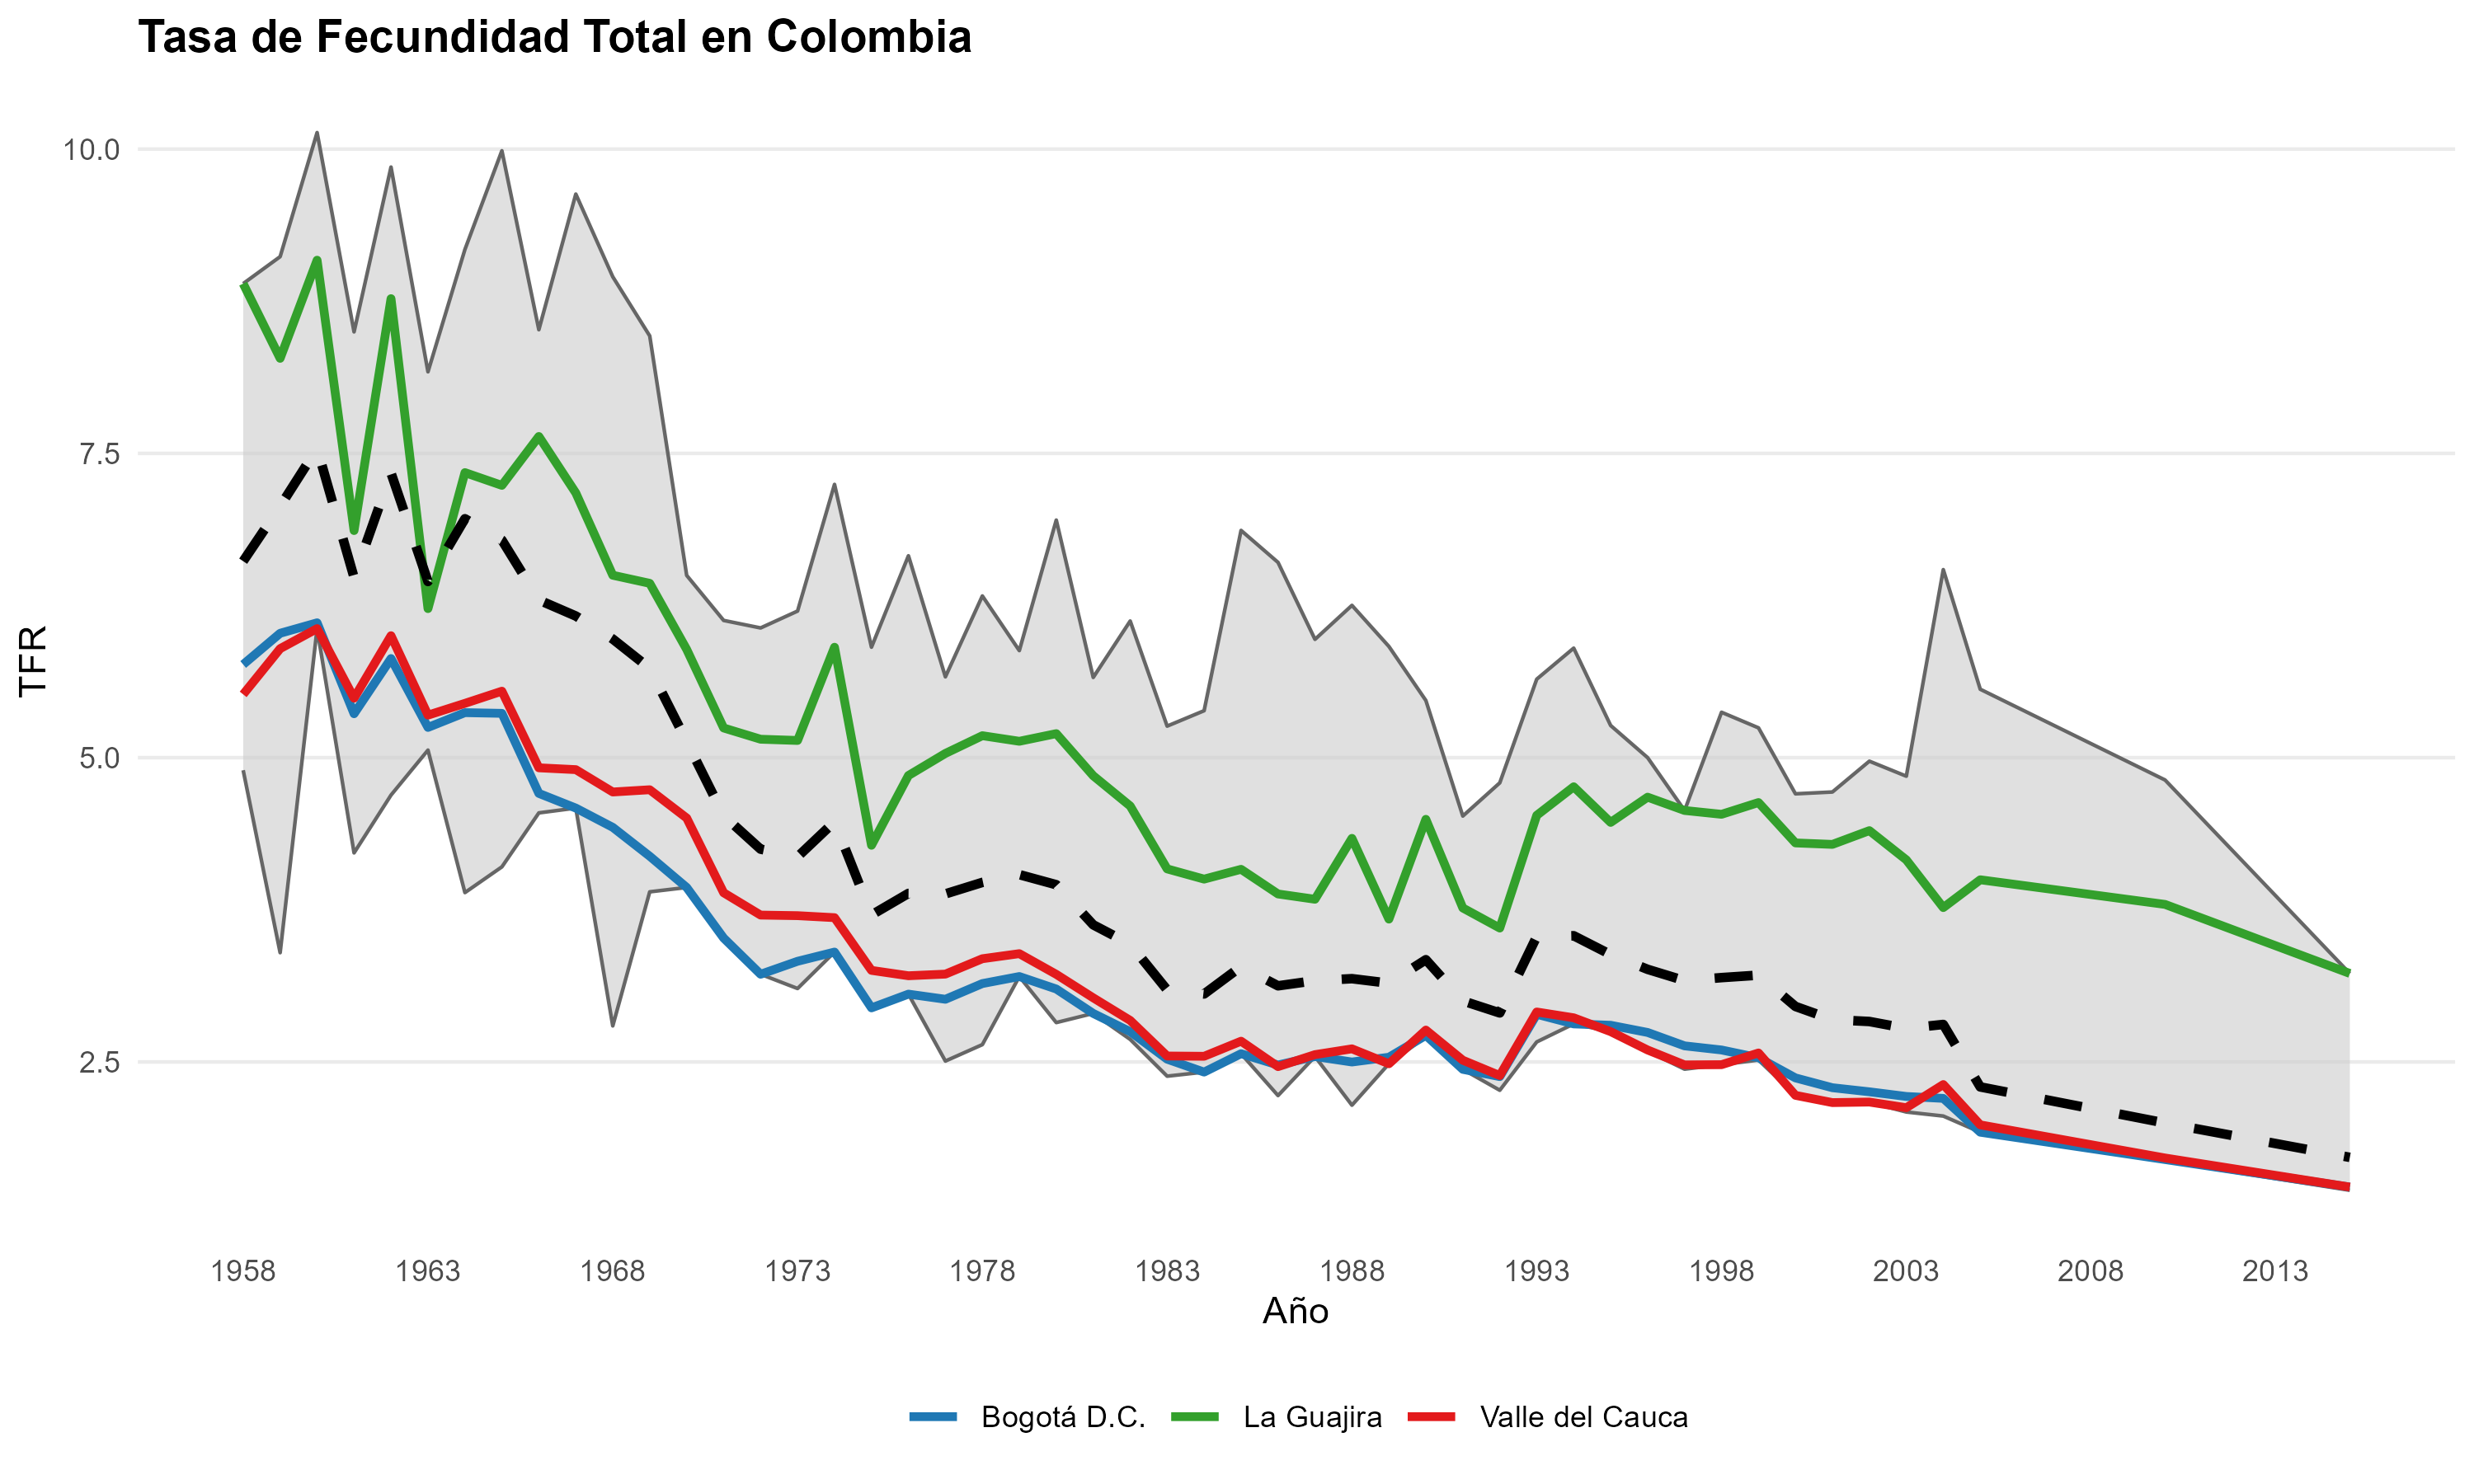
\includegraphics[width=\textwidth]{resumen/tfr_lineas.png}
\end{columns}
\end{frame}

\section{Resultados departamentales: TGF}

\begin{frame}{Veintid\'os transiciones distintas}
\begin{columns}
\column{0.42\textwidth}
En 1960 \alert{todos} los departamentos superaban los 6 hijos por
mujer: desde 6{,}1 en Bogot\'a hasta 10{,}1 en Arauca.
\medskip

La ca\'ida empez\'o en las grandes ciudades y el eje cafetero y se
propag\'o hacia la periferia con d\'ecadas de rezago.
\column{0.58\textwidth}
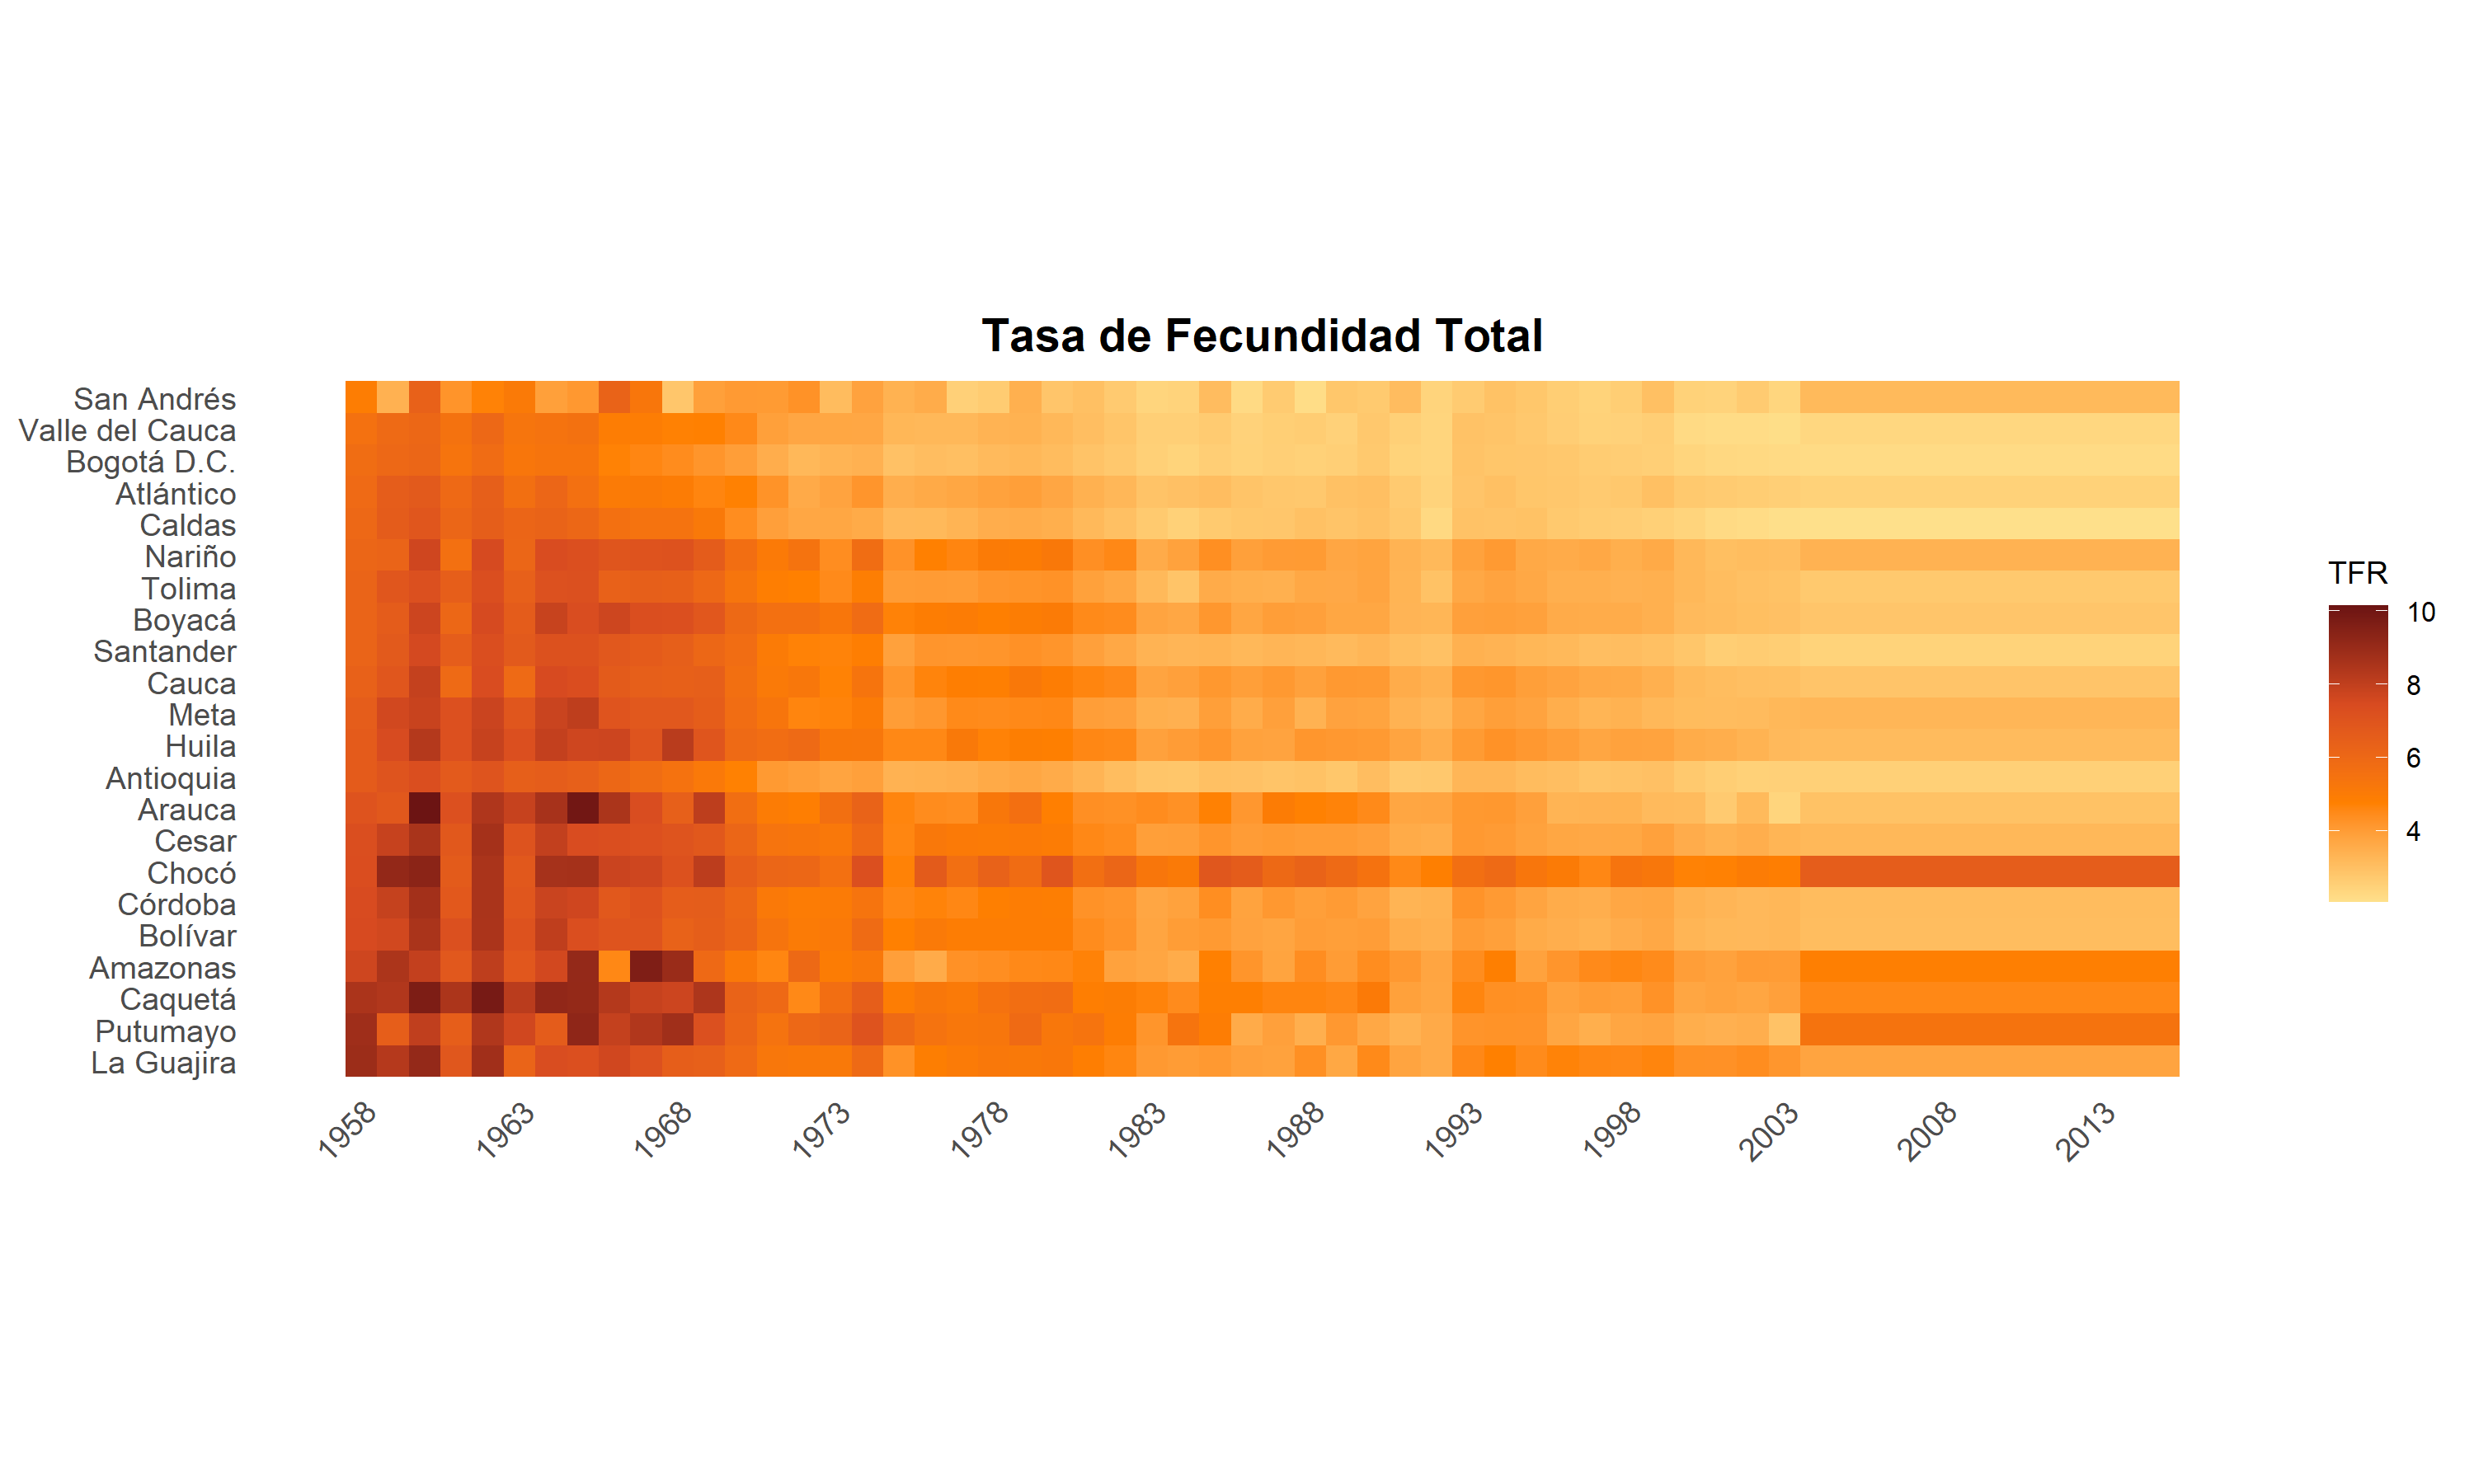
\includegraphics[width=\textwidth]{resumen/tfr_heatmap.png}
\end{columns}
\end{frame}
\begin{frame}{TGF departamental, a\~nos seleccionados}
\begin{center}
{\tiny\begin{tabular}{lccccccc}\toprule
Departamento & 1960 & 1970 & 1980 & 1990 & 2000 & 2004 & 2015$^{*}$ \\ \midrule
Amazonas & 7{,}94 & 5{,}11 & 4{,}54 & 4{,}41 & 3{,}93 & 4{,}82 & 2{,}94 \\
Antioquia & 7{,}31 & 4{,}73 & 3{,}57 & 3{,}06 & 2{,}72 & 2{,}53 & 1{,}40 \\
Arauca & 10{,}14 & 5{,}69 & 4{,}78 & 4{,}49 & 3{,}12 & 2{,}93 & 2{,}13 \\
Atlántico & 6{,}72 & 4{,}73 & 3{,}72 & 3{,}00 & 2{,}73 & 2{,}47 & 1{,}91 \\
Bogotá D.C. & 6{,}11 & 3{,}93 & 3{,}10 & 2{,}72 & 2{,}37 & 2{,}20 & 1{,}40 \\
Bolívar & 8{,}54 & 6{,}14 & 4{,}90 & 3{,}96 & 3{,}31 & 3{,}08 & 2{,}18 \\
Boyacá & 7{,}72 & 5{,}96 & 5{,}01 & 3{,}70 & 3{,}15 & 2{,}83 & 1{,}82 \\
Caldas & 6{,}89 & 4{,}40 & 3{,}47 & 2{,}96 & 2{,}40 & 2{,}06 & 1{,}42 \\
Caquetá & 9{,}68 & 6{,}28 & 5{,}73 & 5{,}04 & 3{,}73 & 4{,}53 & 2{,}12 \\
Cauca & 7{,}91 & 5{,}63 & 4{,}92 & 4{,}06 & 3{,}16 & 2{,}85 & 1{,}91 \\
Cesar & 8{,}57 & 6{,}12 & 4{,}97 & 3{,}90 & 3{,}54 & 3{,}22 & 2{,}17 \\
Chocó & 9{,}33 & 6{,}50 & 6{,}95 & 5{,}47 & 4{,}70 & 6{,}54 & 2{,}92 \\
Córdoba & 8{,}72 & 6{,}03 & 4{,}86 & 3{,}79 & 3{,}39 & 3{,}09 & 2{,}10 \\
Huila & 8{,}31 & 5{,}90 & 4{,}79 & 4{,}05 & 3{,}56 & 3{,}11 & 2{,}08 \\
La Guajira & 9{,}09 & 5{,}89 & 5{,}20 & 4{,}49 & 4{,}30 & 3{,}77 & 3{,}06 \\
Meta & 7{,}82 & 5{,}72 & 4{,}53 & 3{,}78 & 3{,}11 & 3{,}26 & 1{,}88 \\
Nariño & 7{,}67 & 5{,}67 & 5{,}16 & 3{,}79 & 3{,}21 & 3{,}38 & 1{,}63 \\
Putumayo & 8{,}02 & 6{,}15 & 5{,}21 & 3{,}67 & 3{,}51 & 5{,}43 & 1{,}87 \\
San Andrés & 6{,}34 & 4{,}05 & 2{,}82 & 2{,}71 & 2{,}48 & 3{,}16 & 1{,}73 \\
Santander & 7{,}53 & 5{,}72 & 4{,}19 & 3{,}26 & 2{,}82 & 2{,}45 & 1{,}72 \\
Tolima & 7{,}22 & 5{,}34 & 4{,}26 & 3{,}77 & 3{,}22 & 2{,}72 & 1{,}80 \\
Valle del Cauca & 6{,}06 & 4{,}50 & 3{,}22 & 2{,}76 & 2{,}23 & 2{,}31 & 1{,}43 \\
\bottomrule\end{tabular}}
\end{center}
{\scriptsize $^{*}$2015: retrospecci\'on del CNPV 2018 (edad quinquenal,
v\'inculo imputado). Fuente: c\'alculos propios.}
\end{frame}

\begin{frame}{Convergencia con una periferia persistente}
El rango departamental se comprime de 4 hijos de diferencia en 1960
(6{,}1,10{,}1) a cerca de 1{,}7 en 2015 (1{,}4,3{,}1): hay
convergencia en niveles.
\bigskip

Pero el \alert{orden casi no cambia}: Choc\'o, la Amazon\'ia, La
Guajira y Putumayo, que ten\'ian la fecundidad m\'as alta en 1960, son
los mismos rezagados de hoy. Y n\'otese el repunte at\'ipico de varios
de ellos en 2004 (Choc\'o 6{,}5; Putumayo 5{,}4).
\bigskip

{\small Pendiente: pruebas formales de convergencia; hip\'otesis
geogr\'afica (densidad poblacional por a\~no censal, departamentos de
cordillera sin espacio de expansi\'on).}
\end{frame}

\begin{frame}{A continuaci\'on: la transici\'on departamento por departamento}
Las siguientes 22 diapositivas muestran la serie completa de TGF de cada
agrupaci\'on departamental frente al promedio nacional. Para la
discusi\'on de hoy interesan especialmente:
\begin{itemize}
\item \alert{San Andr\'es}: transici\'on temprana y repunte posterior.
\item \alert{Choc\'o, Putumayo, Amazonas}: rezago persistente y saltos en 2004.
\item \alert{Bogot\'a, Caldas, Valle}: los l\'ideres de la ca\'ida.
\end{itemize}
\end{frame}
\begin{frame}{TGF: Amazonas}
\begin{center}
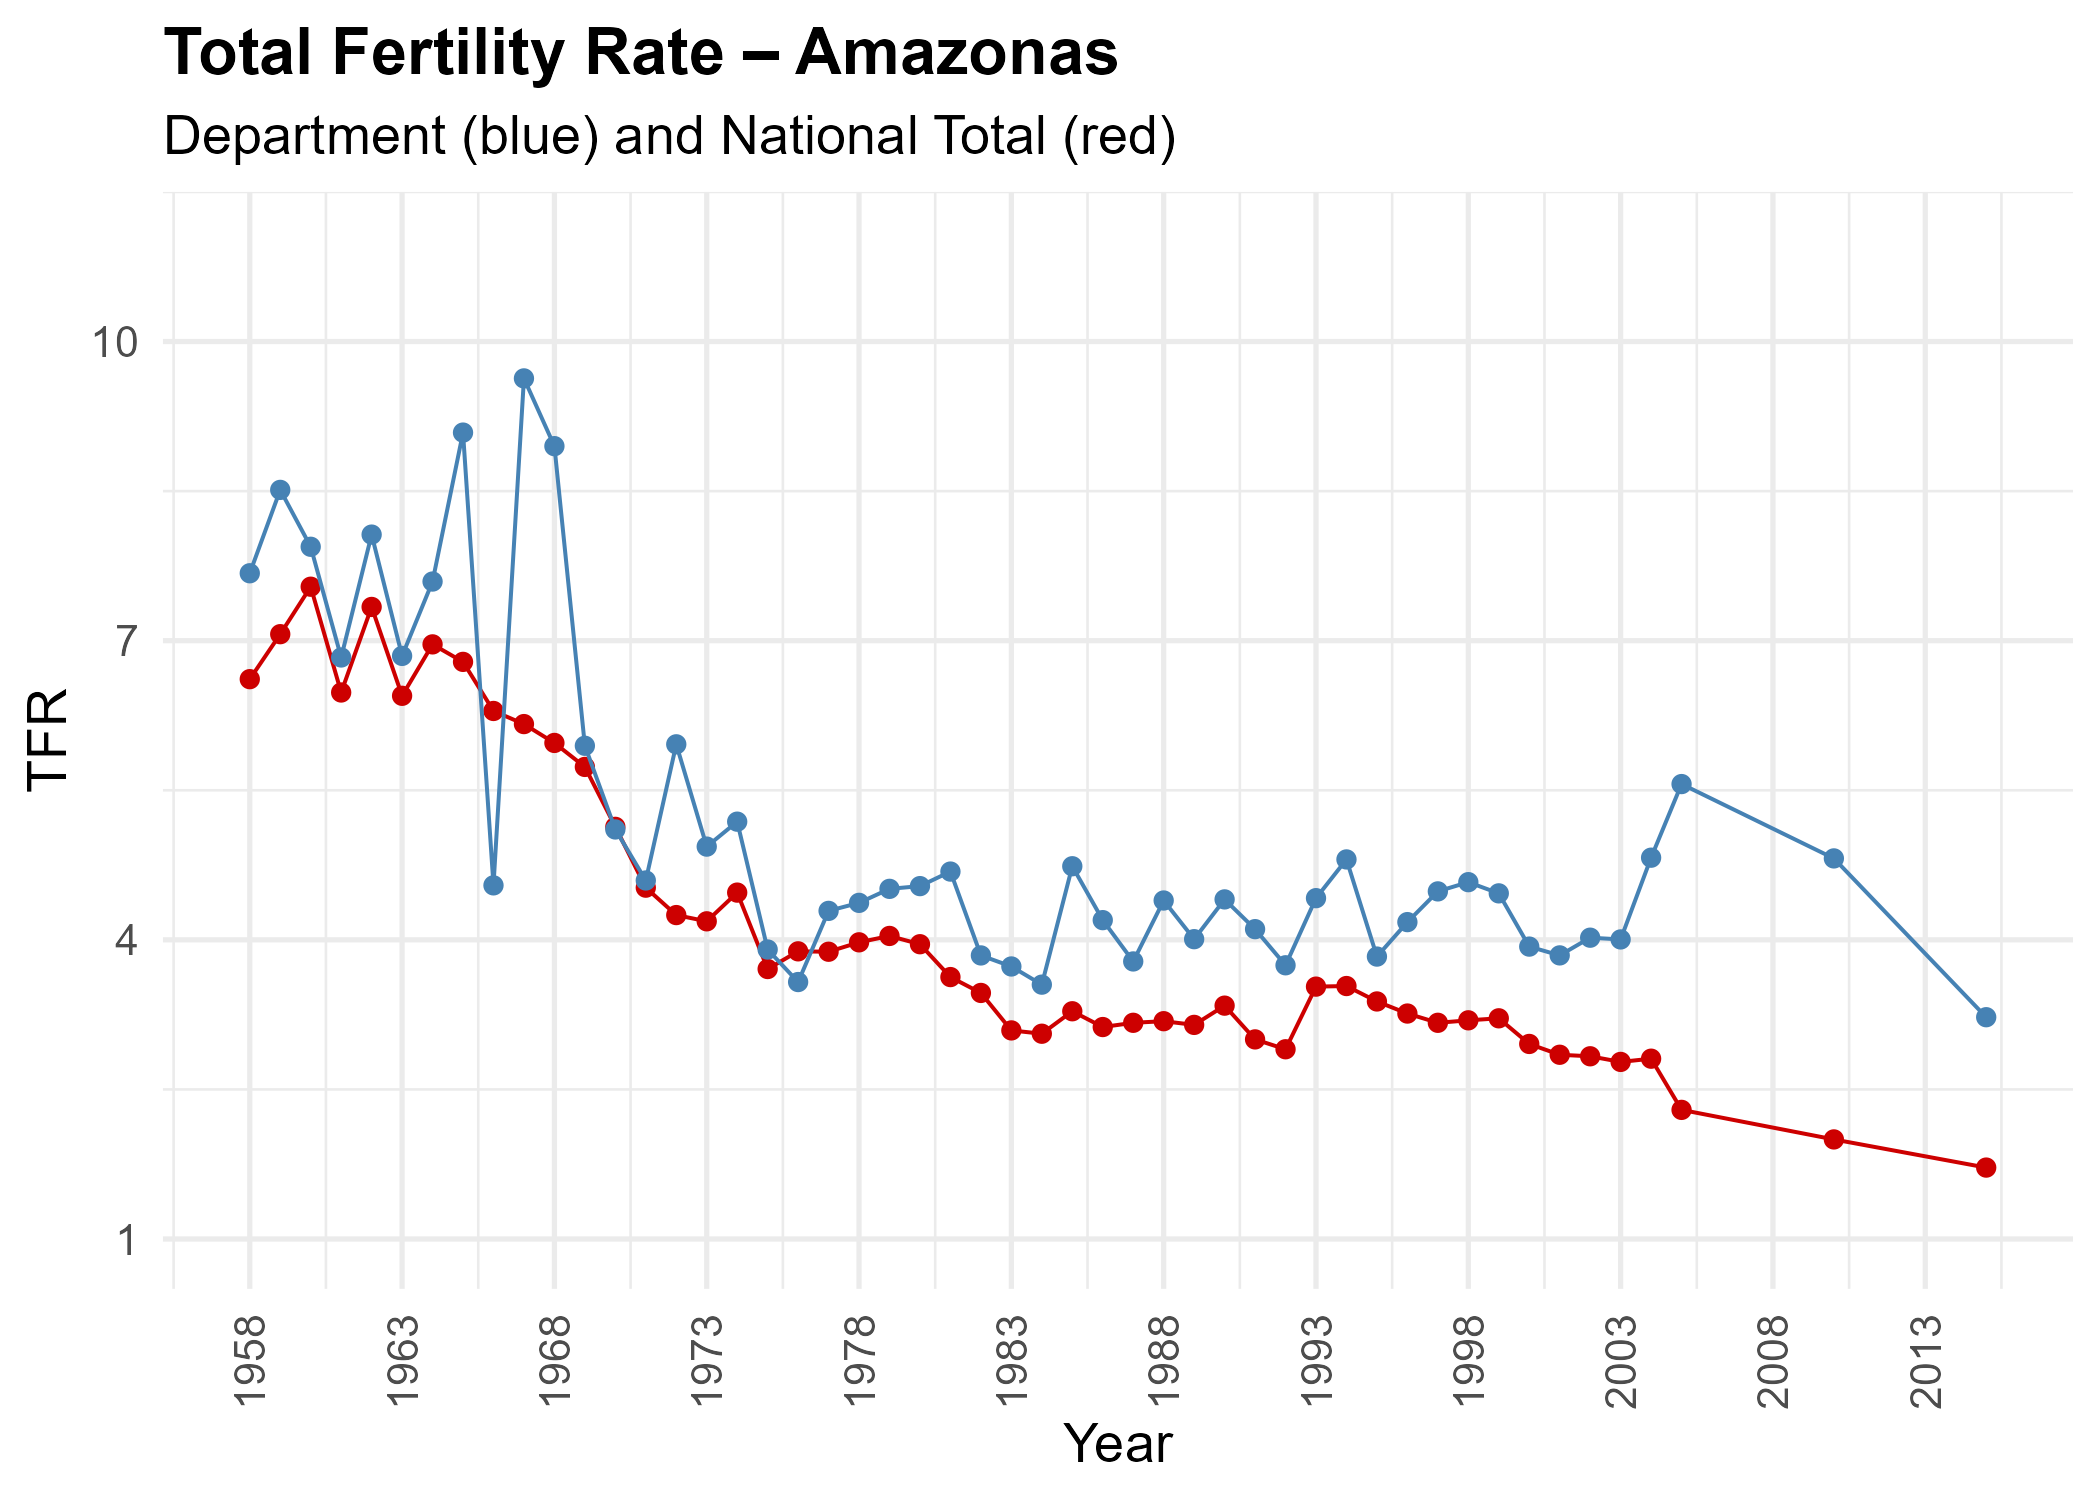
\includegraphics[height=0.78\textheight]{tfr_departamental/TFR_Amazonas_vs_National.png}
\end{center}
\end{frame}
\begin{frame}{TGF: Antioquia}
\begin{center}
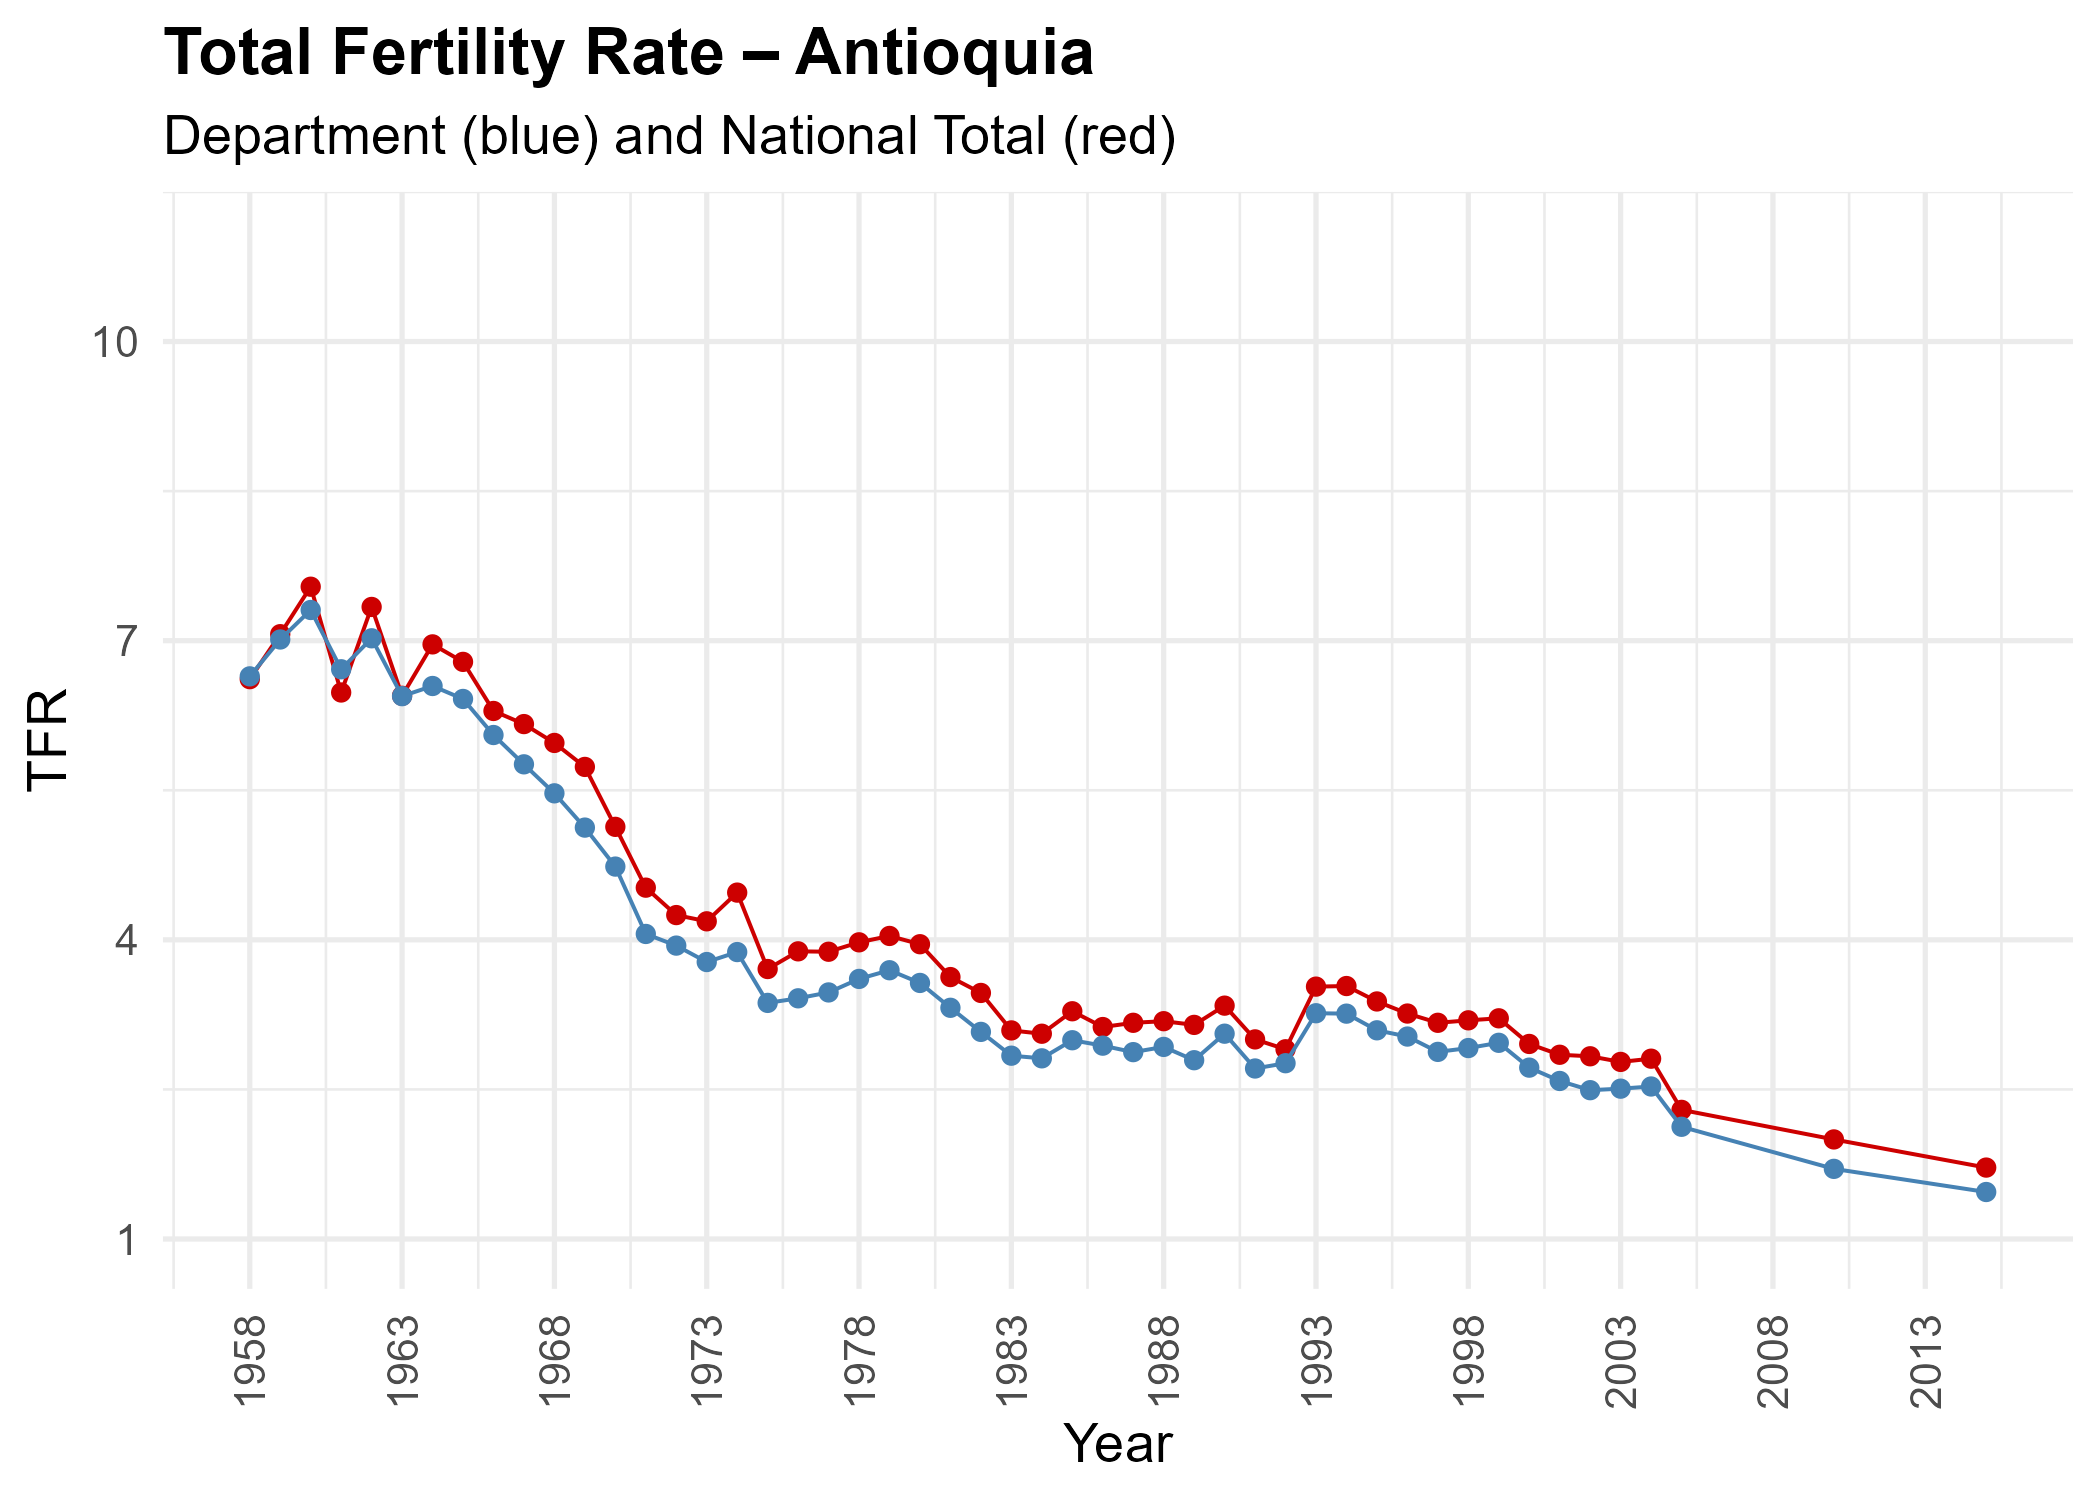
\includegraphics[height=0.78\textheight]{tfr_departamental/TFR_Antioquia_vs_National.png}
\end{center}
\end{frame}
\begin{frame}{TGF: Arauca}
\begin{center}
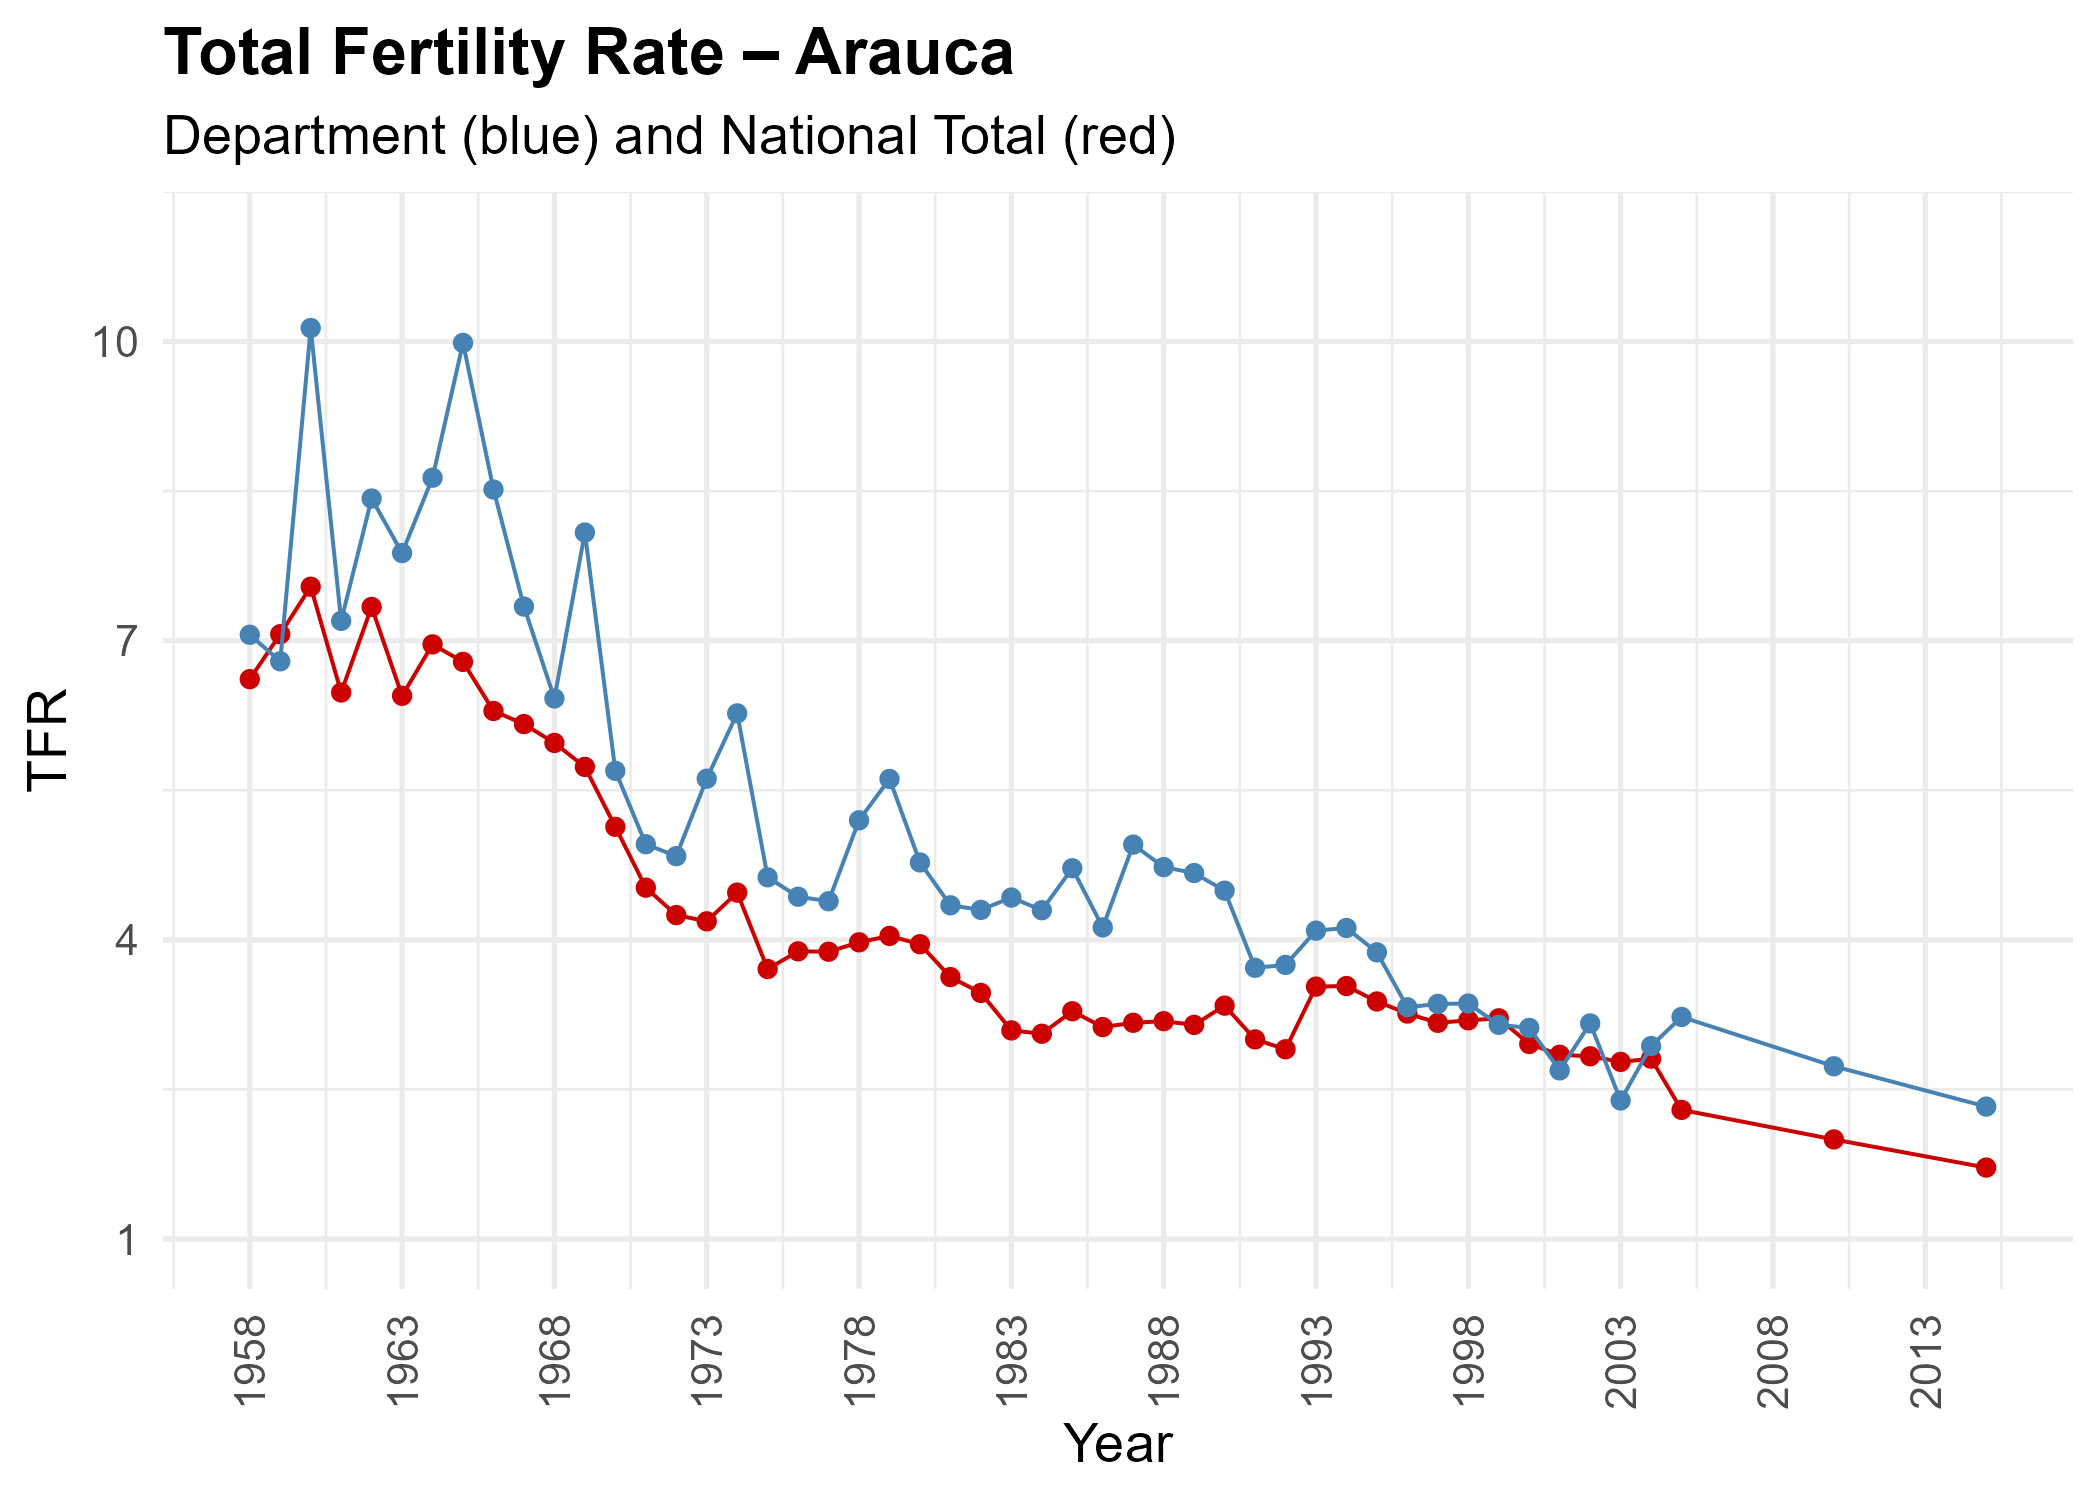
\includegraphics[height=0.78\textheight]{tfr_departamental/TFR_Arauca_vs_National.png}
\end{center}
\end{frame}
\begin{frame}{TGF: Atlántico}
\begin{center}
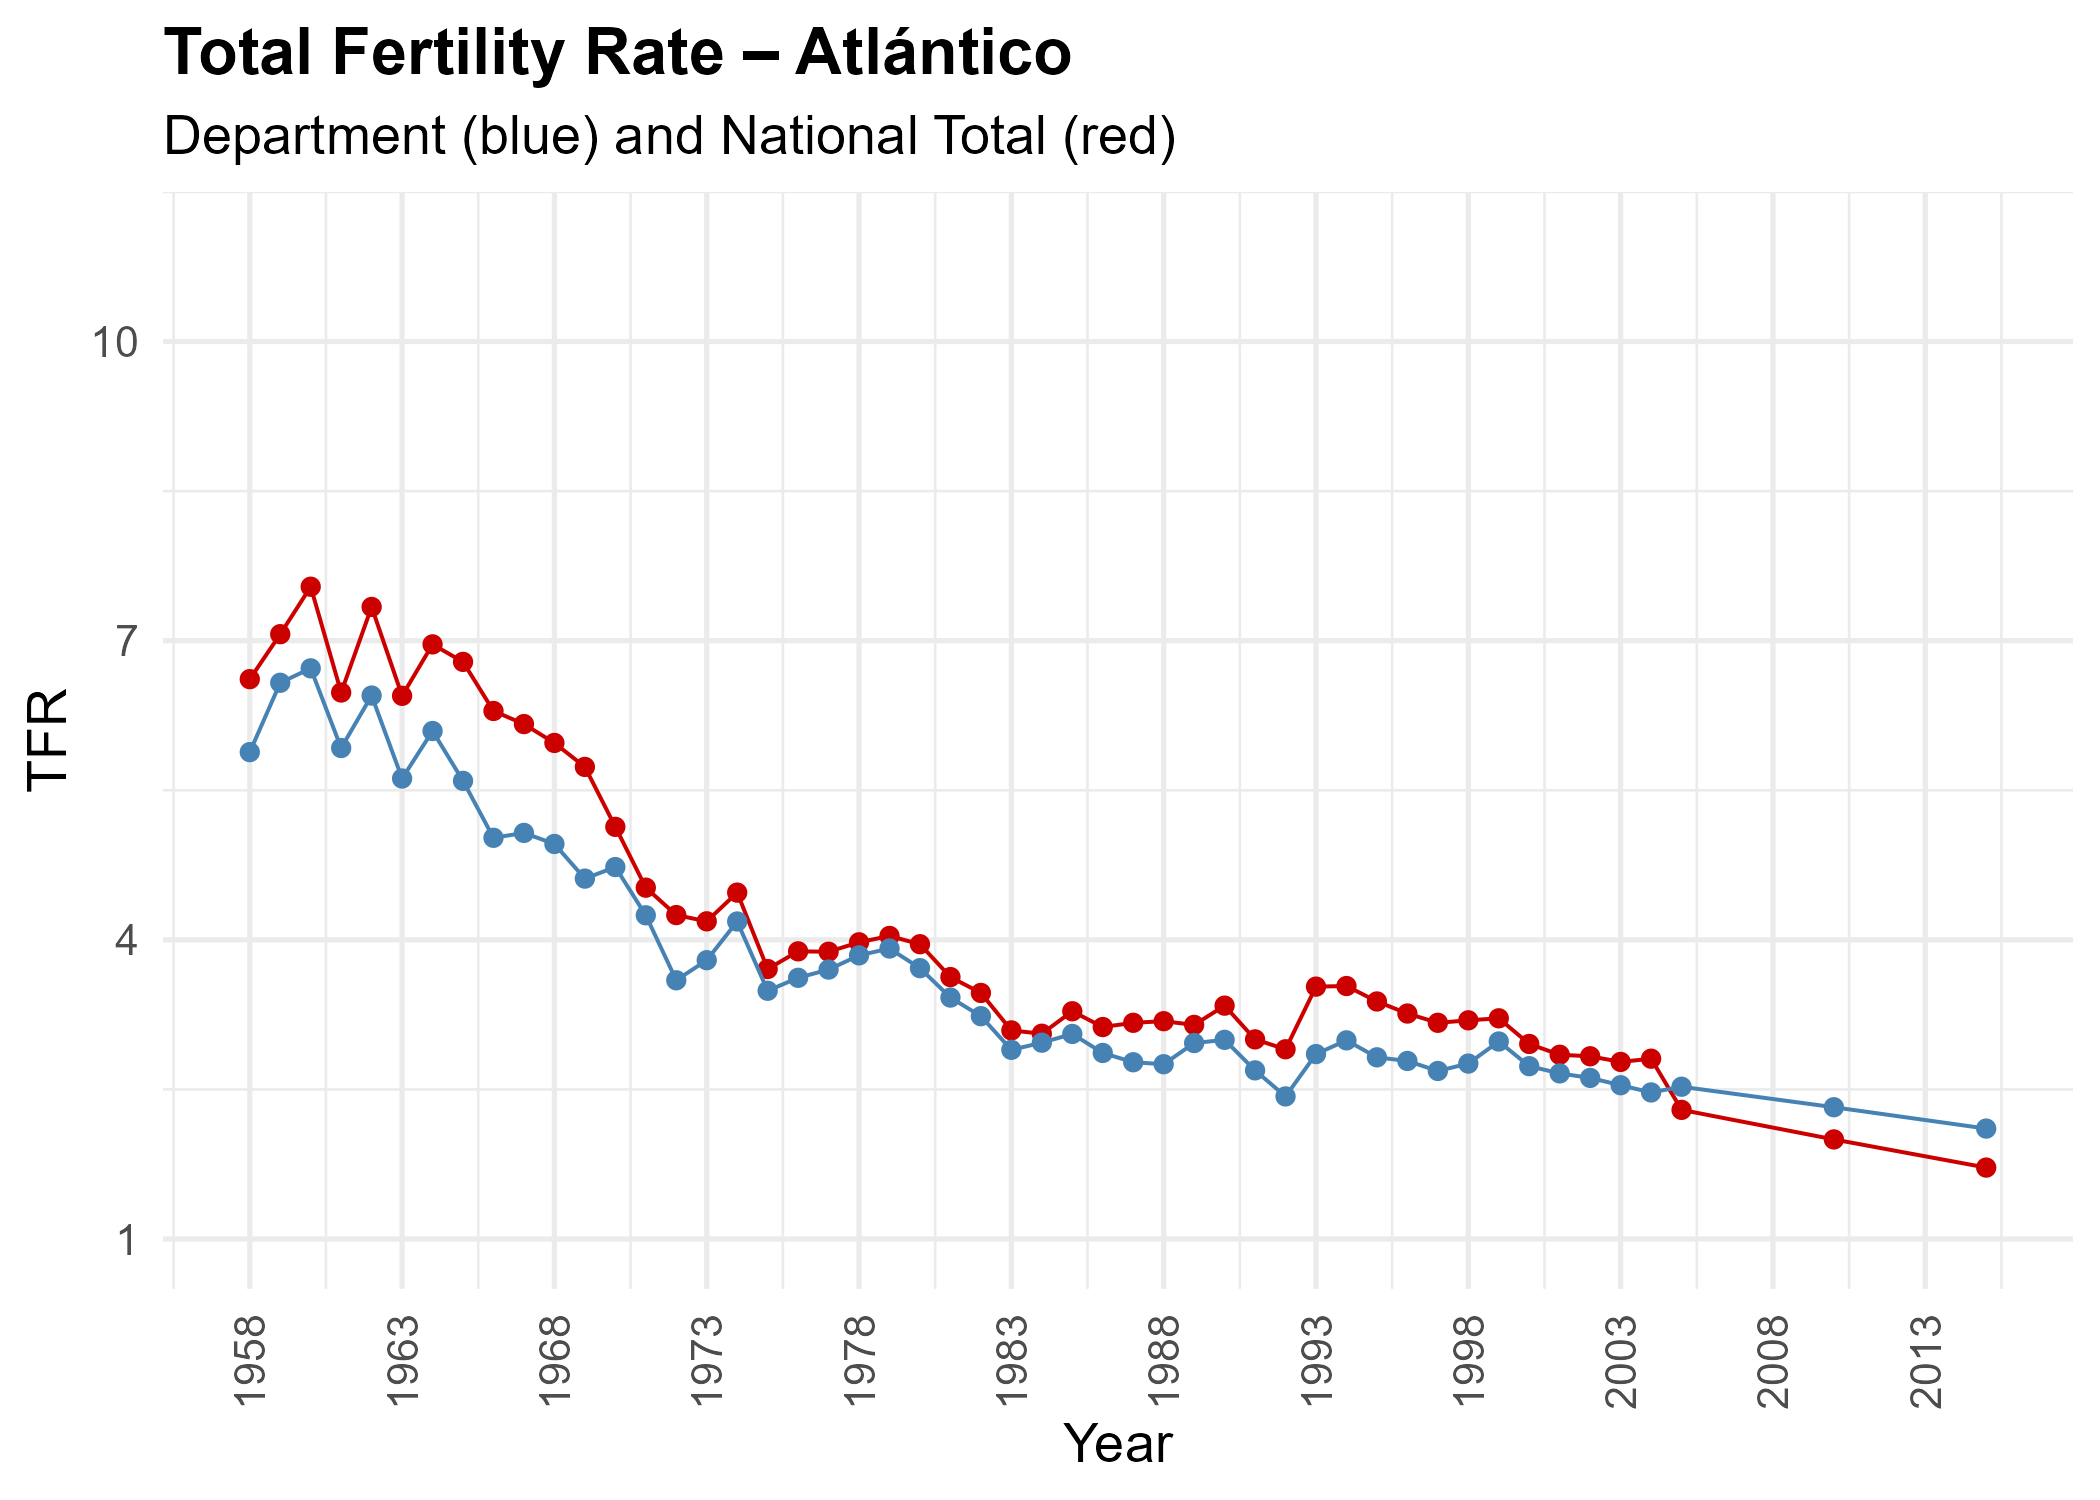
\includegraphics[height=0.78\textheight]{tfr_departamental/TFR_Atlántico_vs_National.png}
\end{center}
\end{frame}
\begin{frame}{TGF: Bogotá D.C.}
\begin{center}
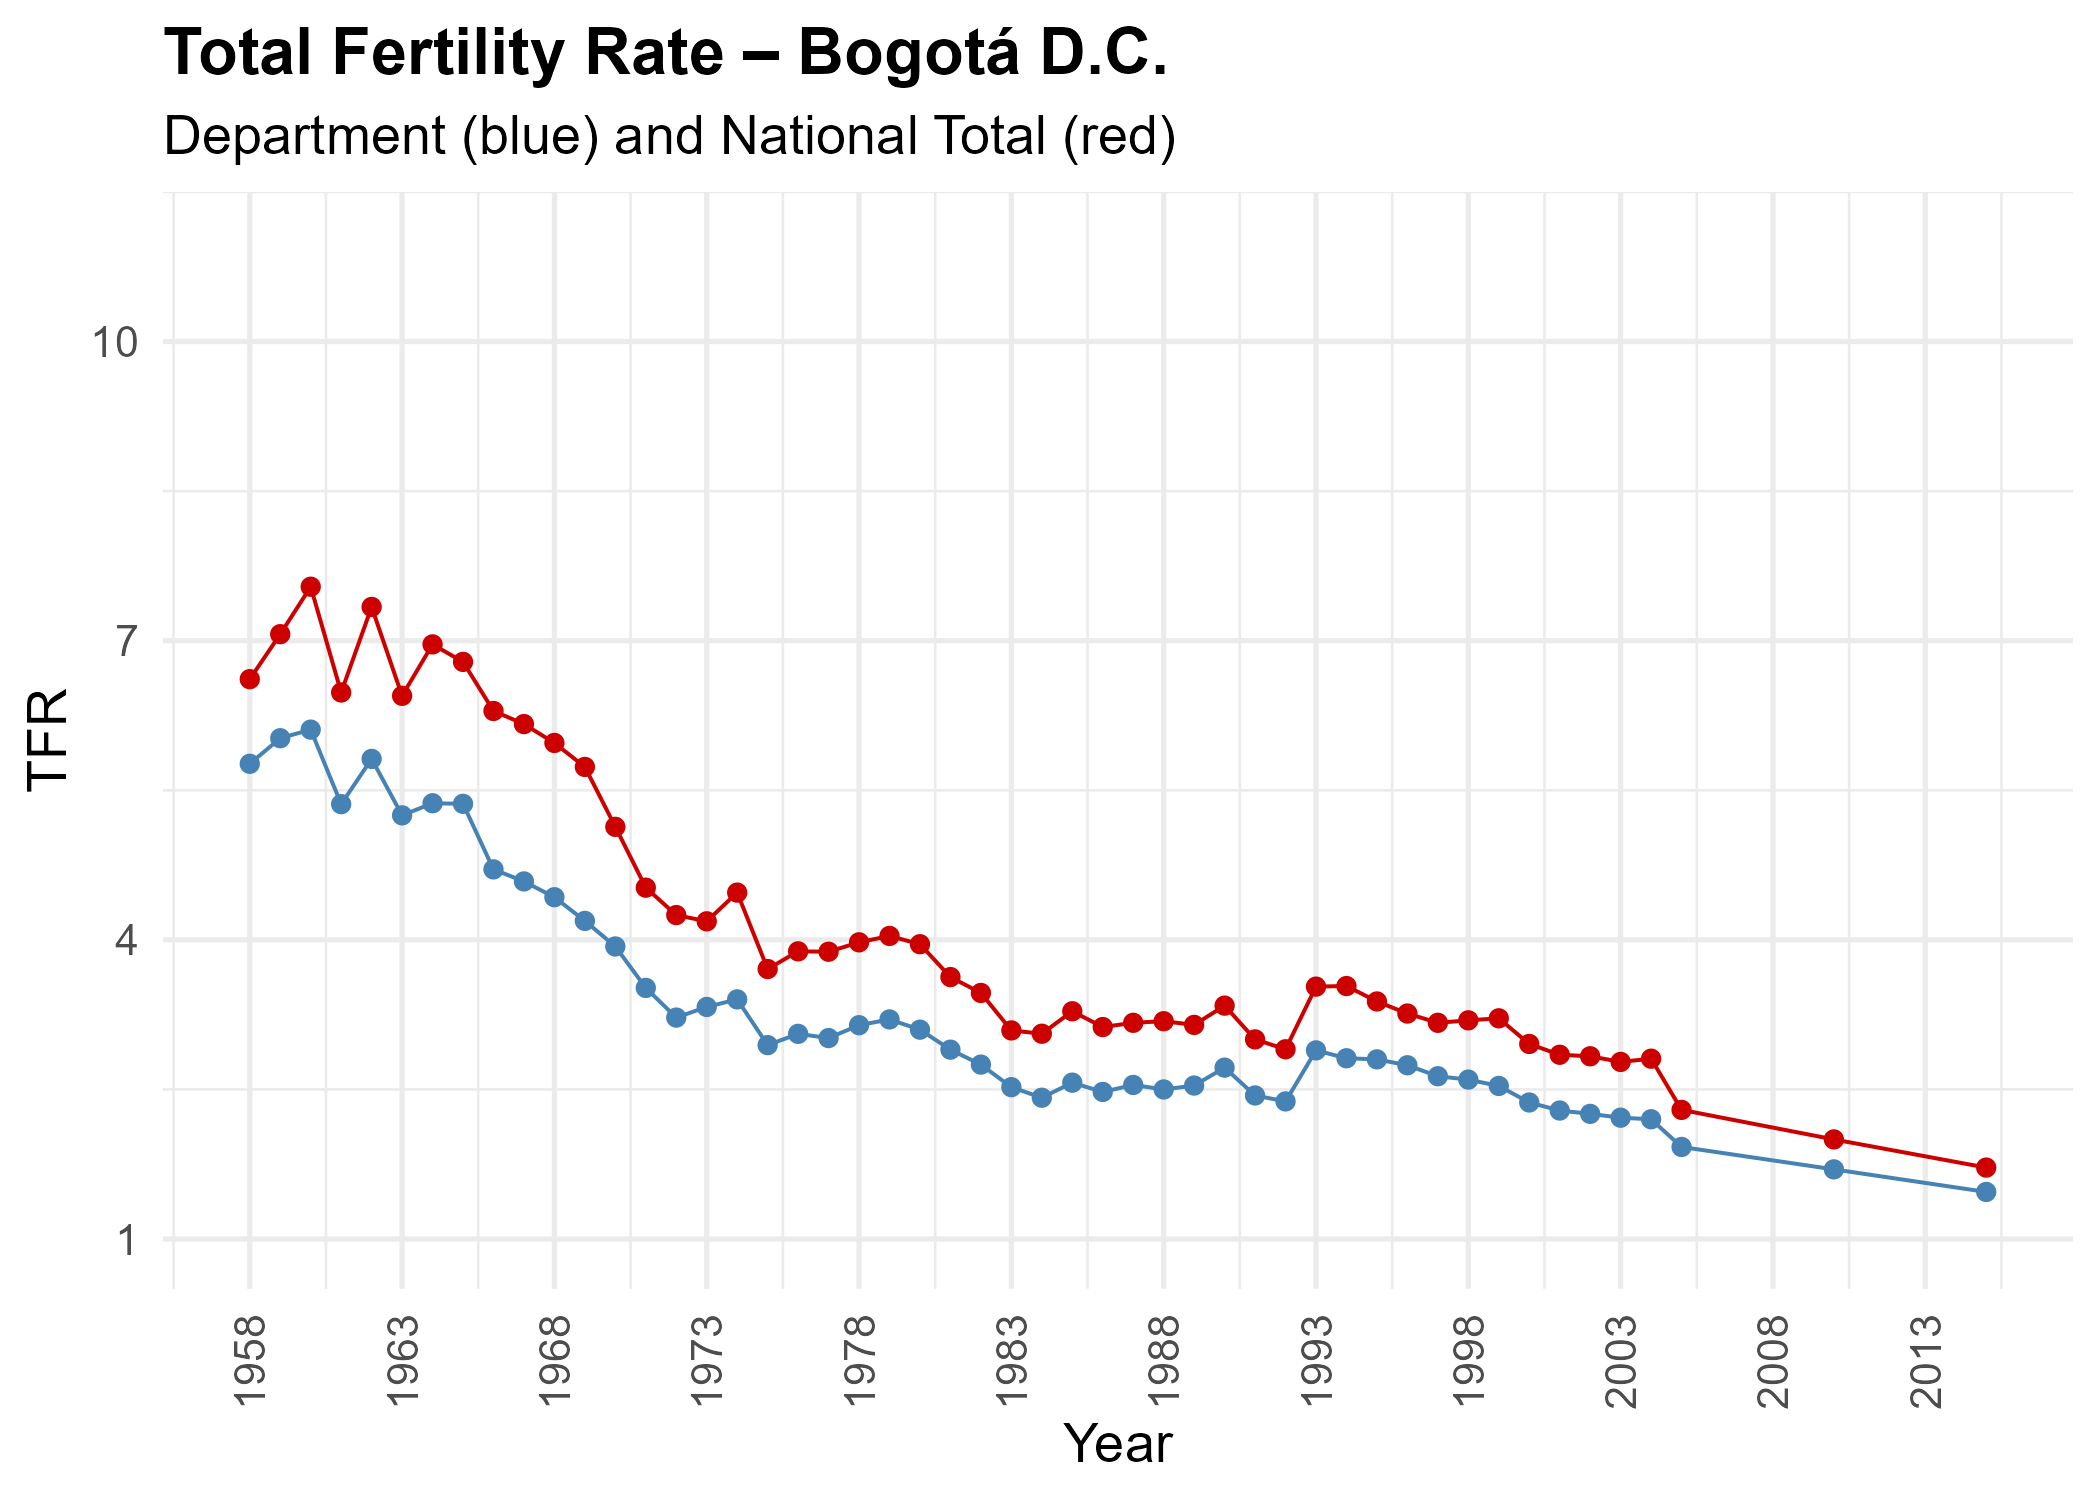
\includegraphics[height=0.78\textheight]{tfr_departamental/TFR_Bogotá D.C._vs_National.png}
\end{center}
\end{frame}
\begin{frame}{TGF: Bolívar}
\begin{center}
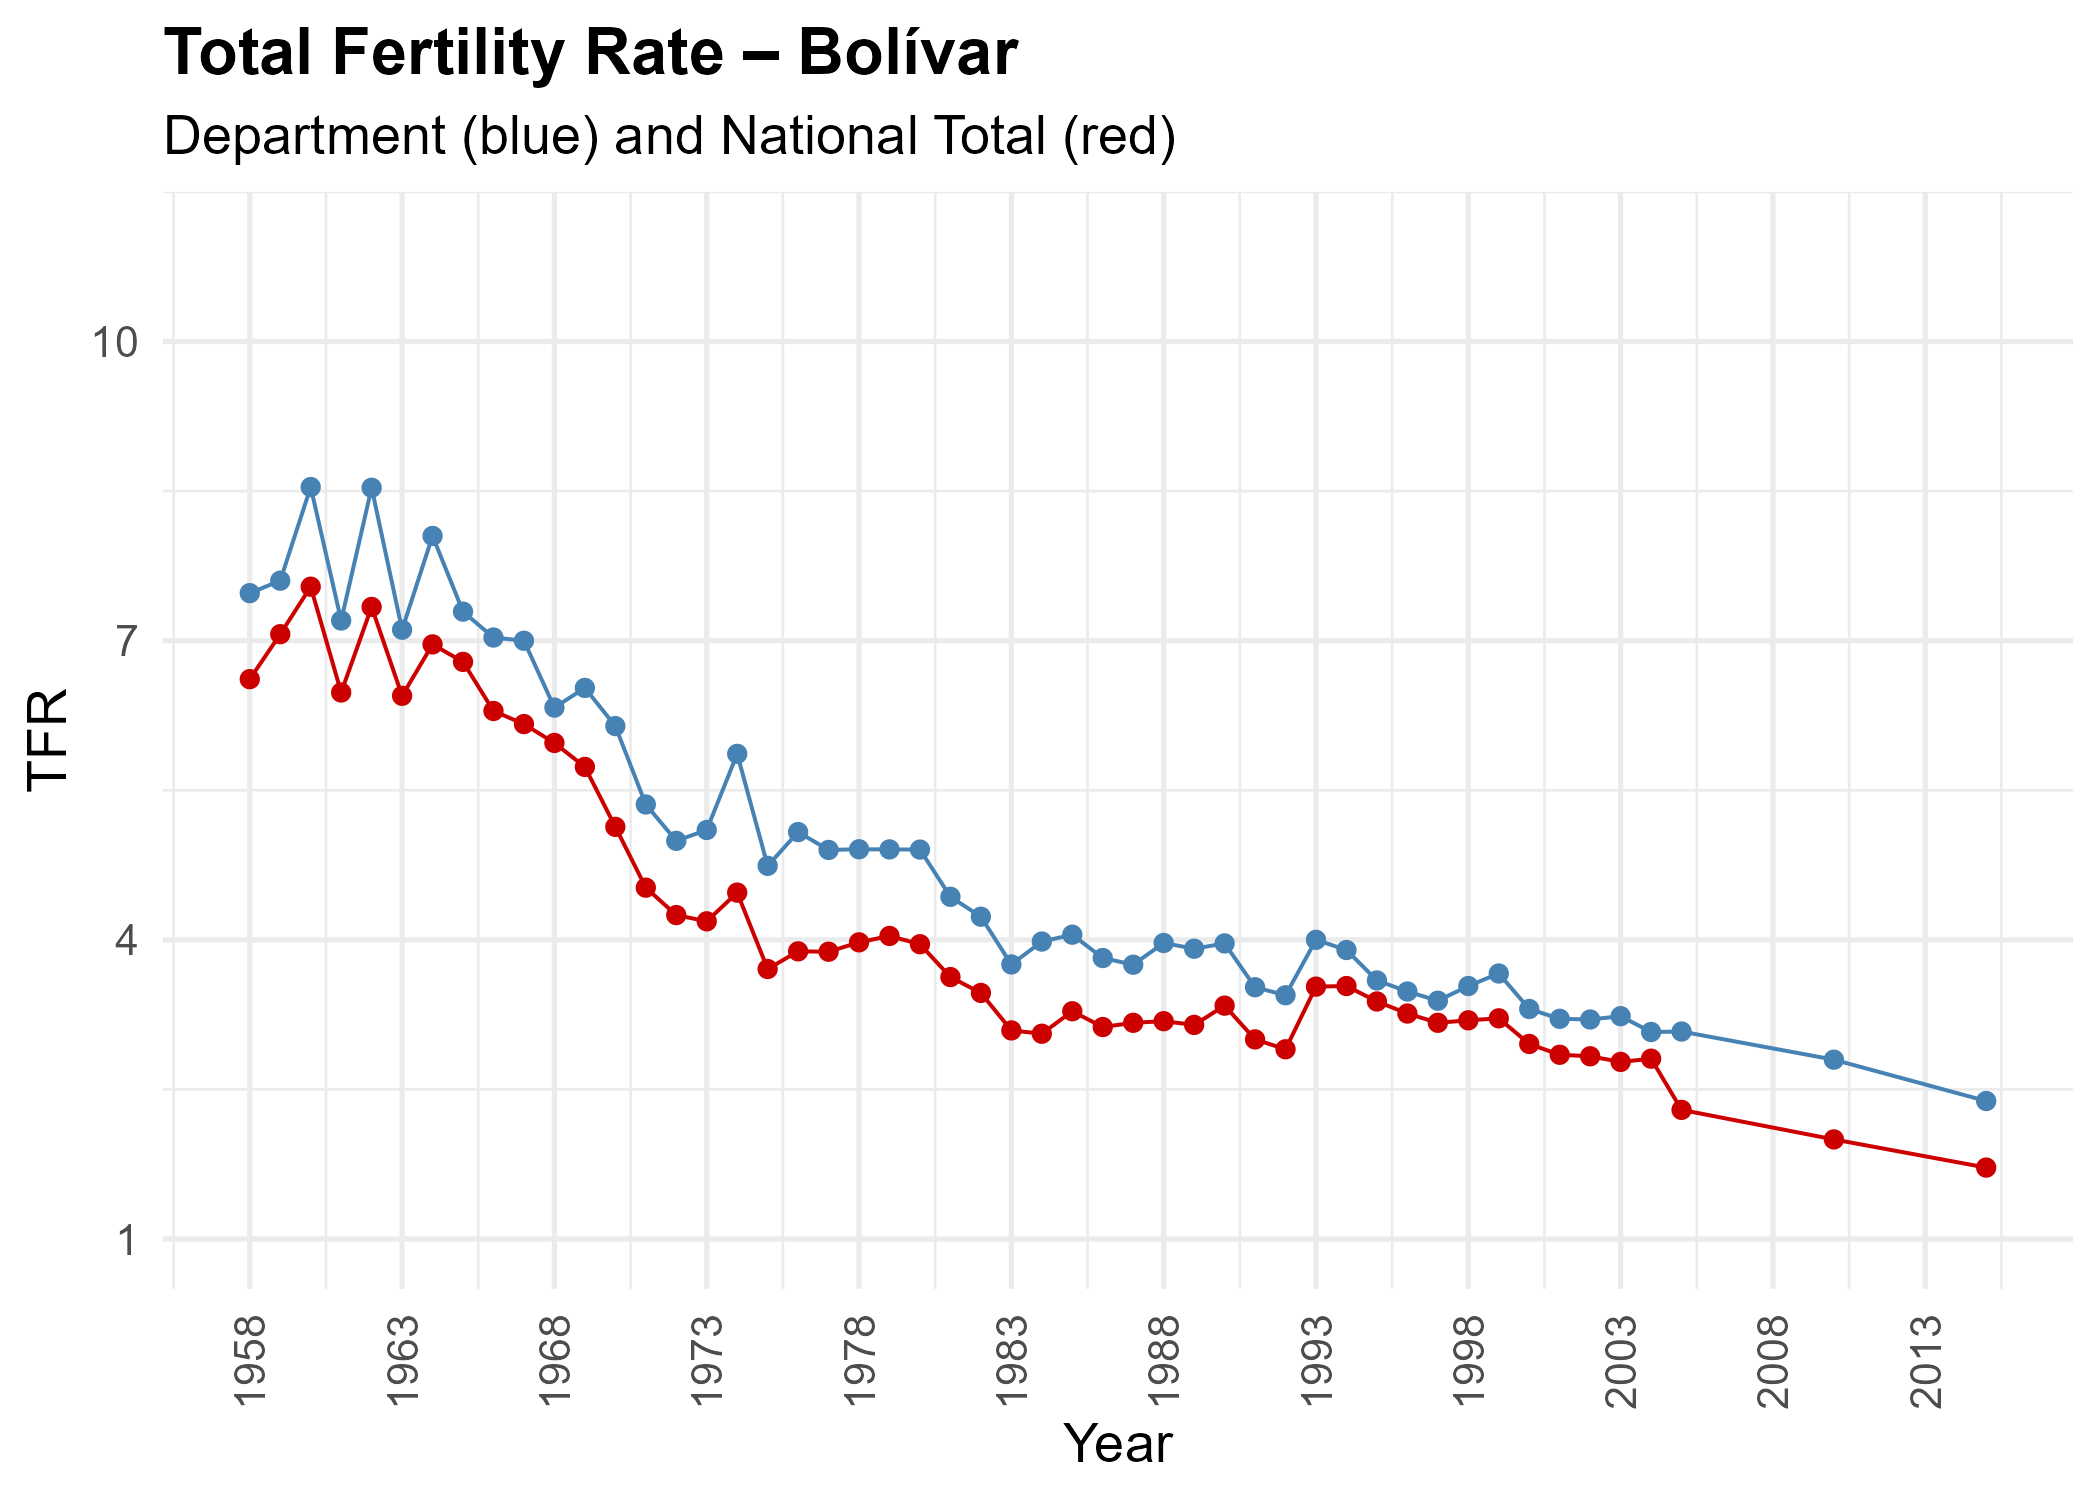
\includegraphics[height=0.78\textheight]{tfr_departamental/TFR_Bolívar_vs_National.png}
\end{center}
\end{frame}
\begin{frame}{TGF: Boyacá}
\begin{center}
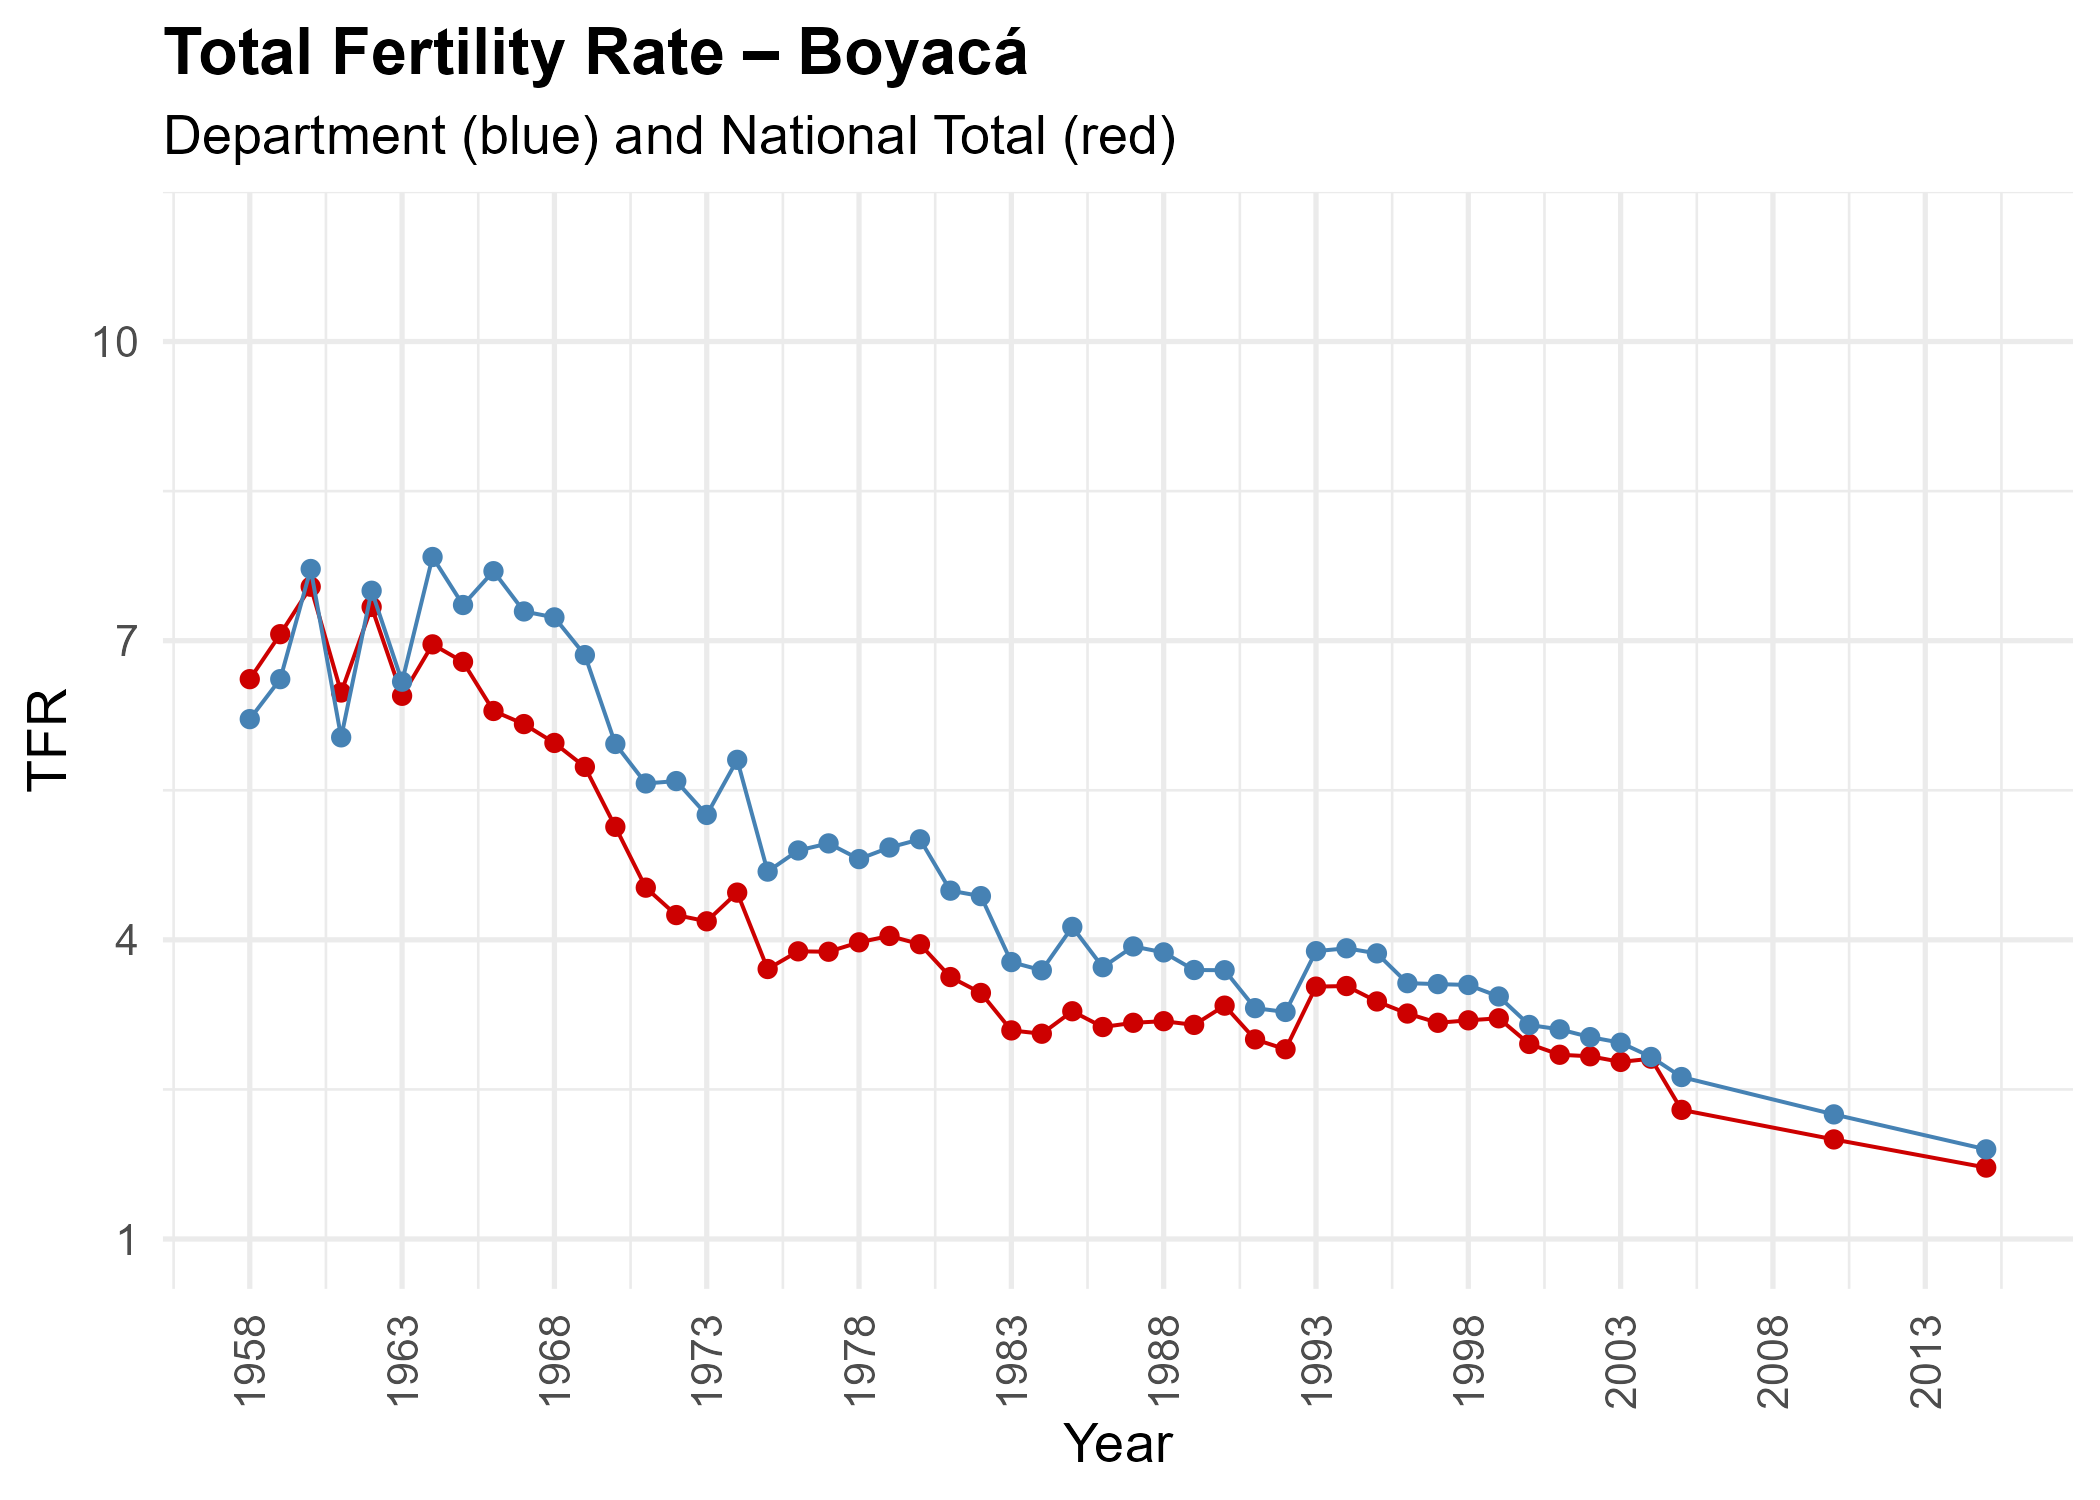
\includegraphics[height=0.78\textheight]{tfr_departamental/TFR_Boyacá_vs_National.png}
\end{center}
\end{frame}
\begin{frame}{TGF: Caldas}
\begin{center}
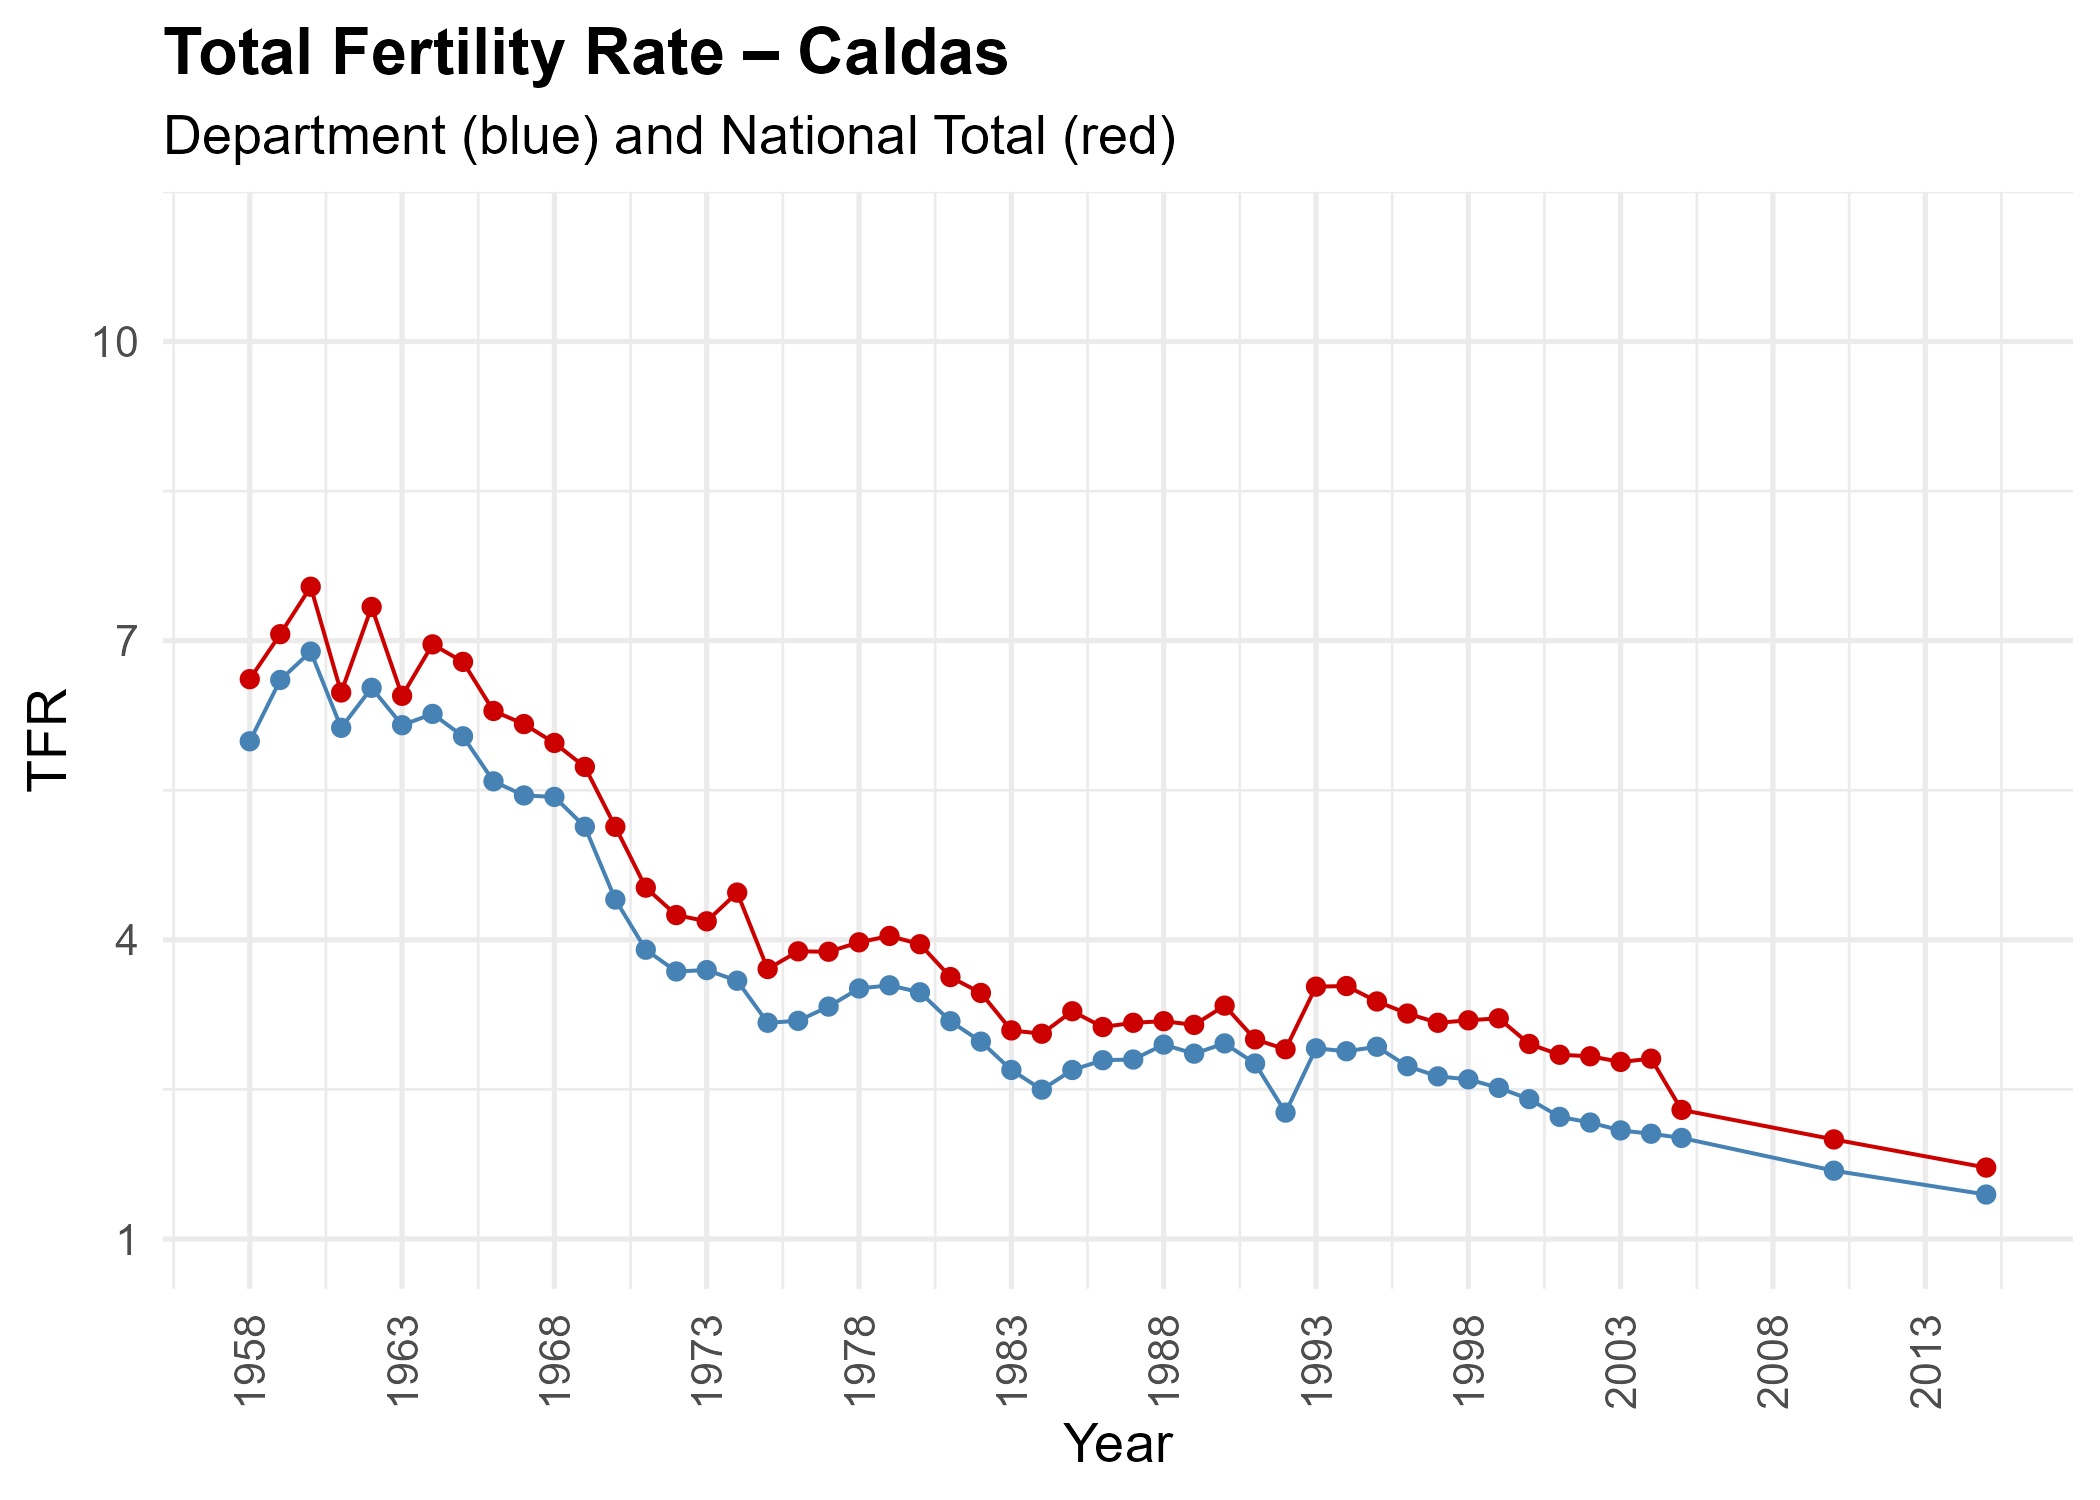
\includegraphics[height=0.78\textheight]{tfr_departamental/TFR_Caldas_vs_National.png}
\end{center}
\end{frame}
\begin{frame}{TGF: Caquetá}
\begin{center}
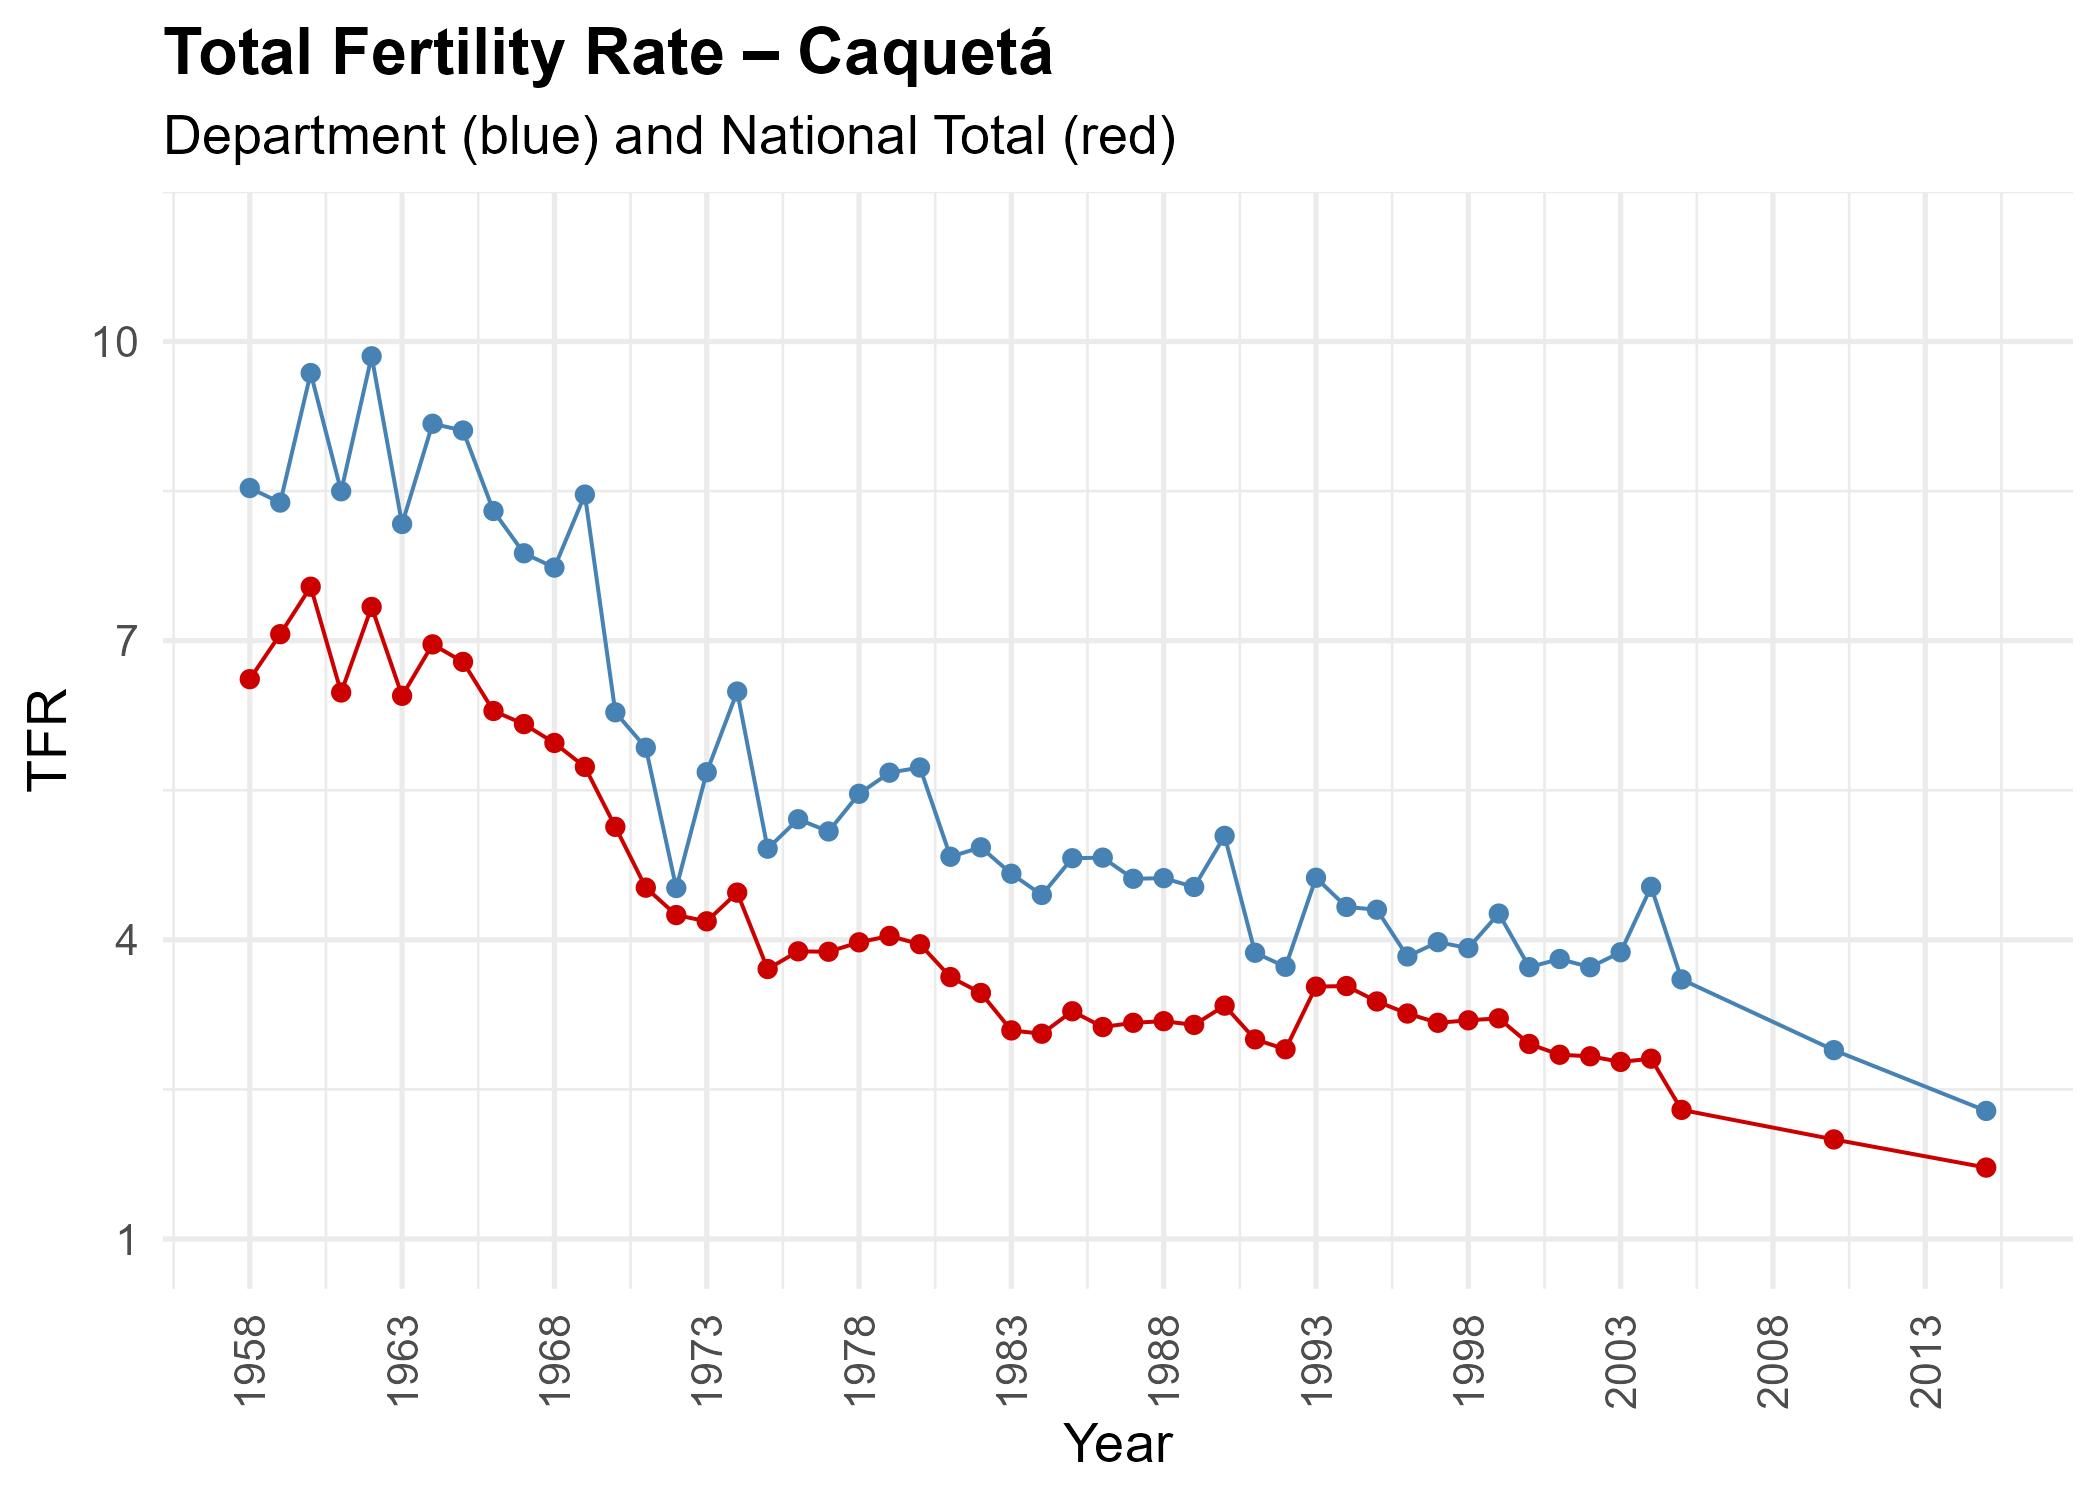
\includegraphics[height=0.78\textheight]{tfr_departamental/TFR_Caquetá_vs_National.png}
\end{center}
\end{frame}
\begin{frame}{TGF: Cauca}
\begin{center}
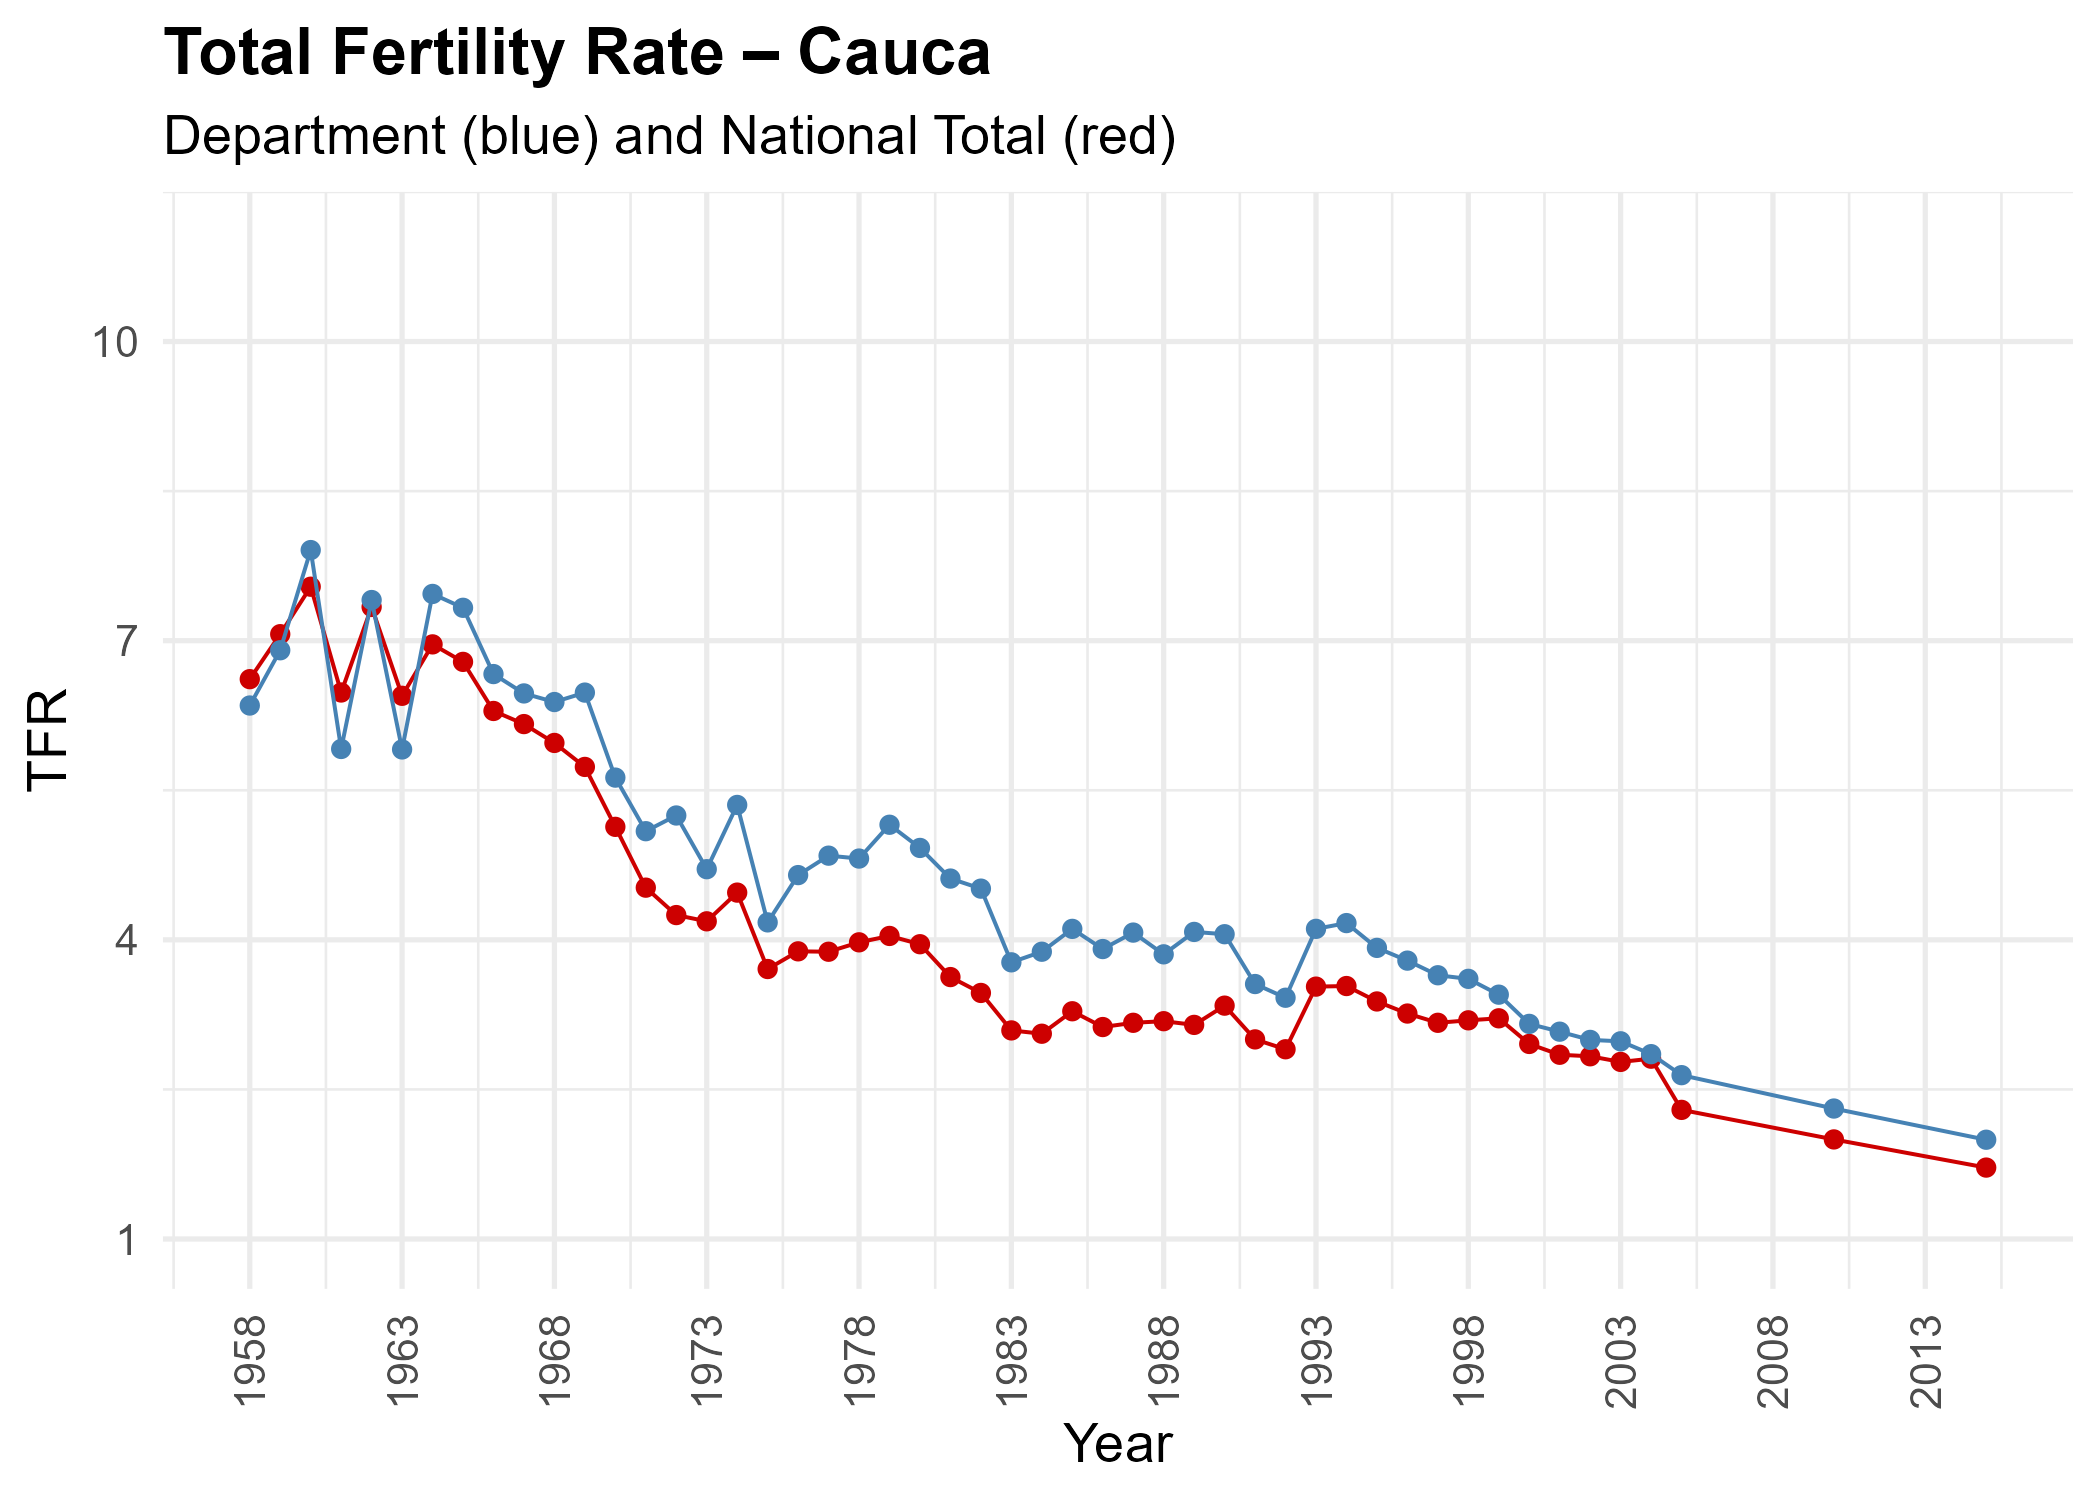
\includegraphics[height=0.78\textheight]{tfr_departamental/TFR_Cauca_vs_National.png}
\end{center}
\end{frame}
\begin{frame}{TGF: Cesar}
\begin{center}
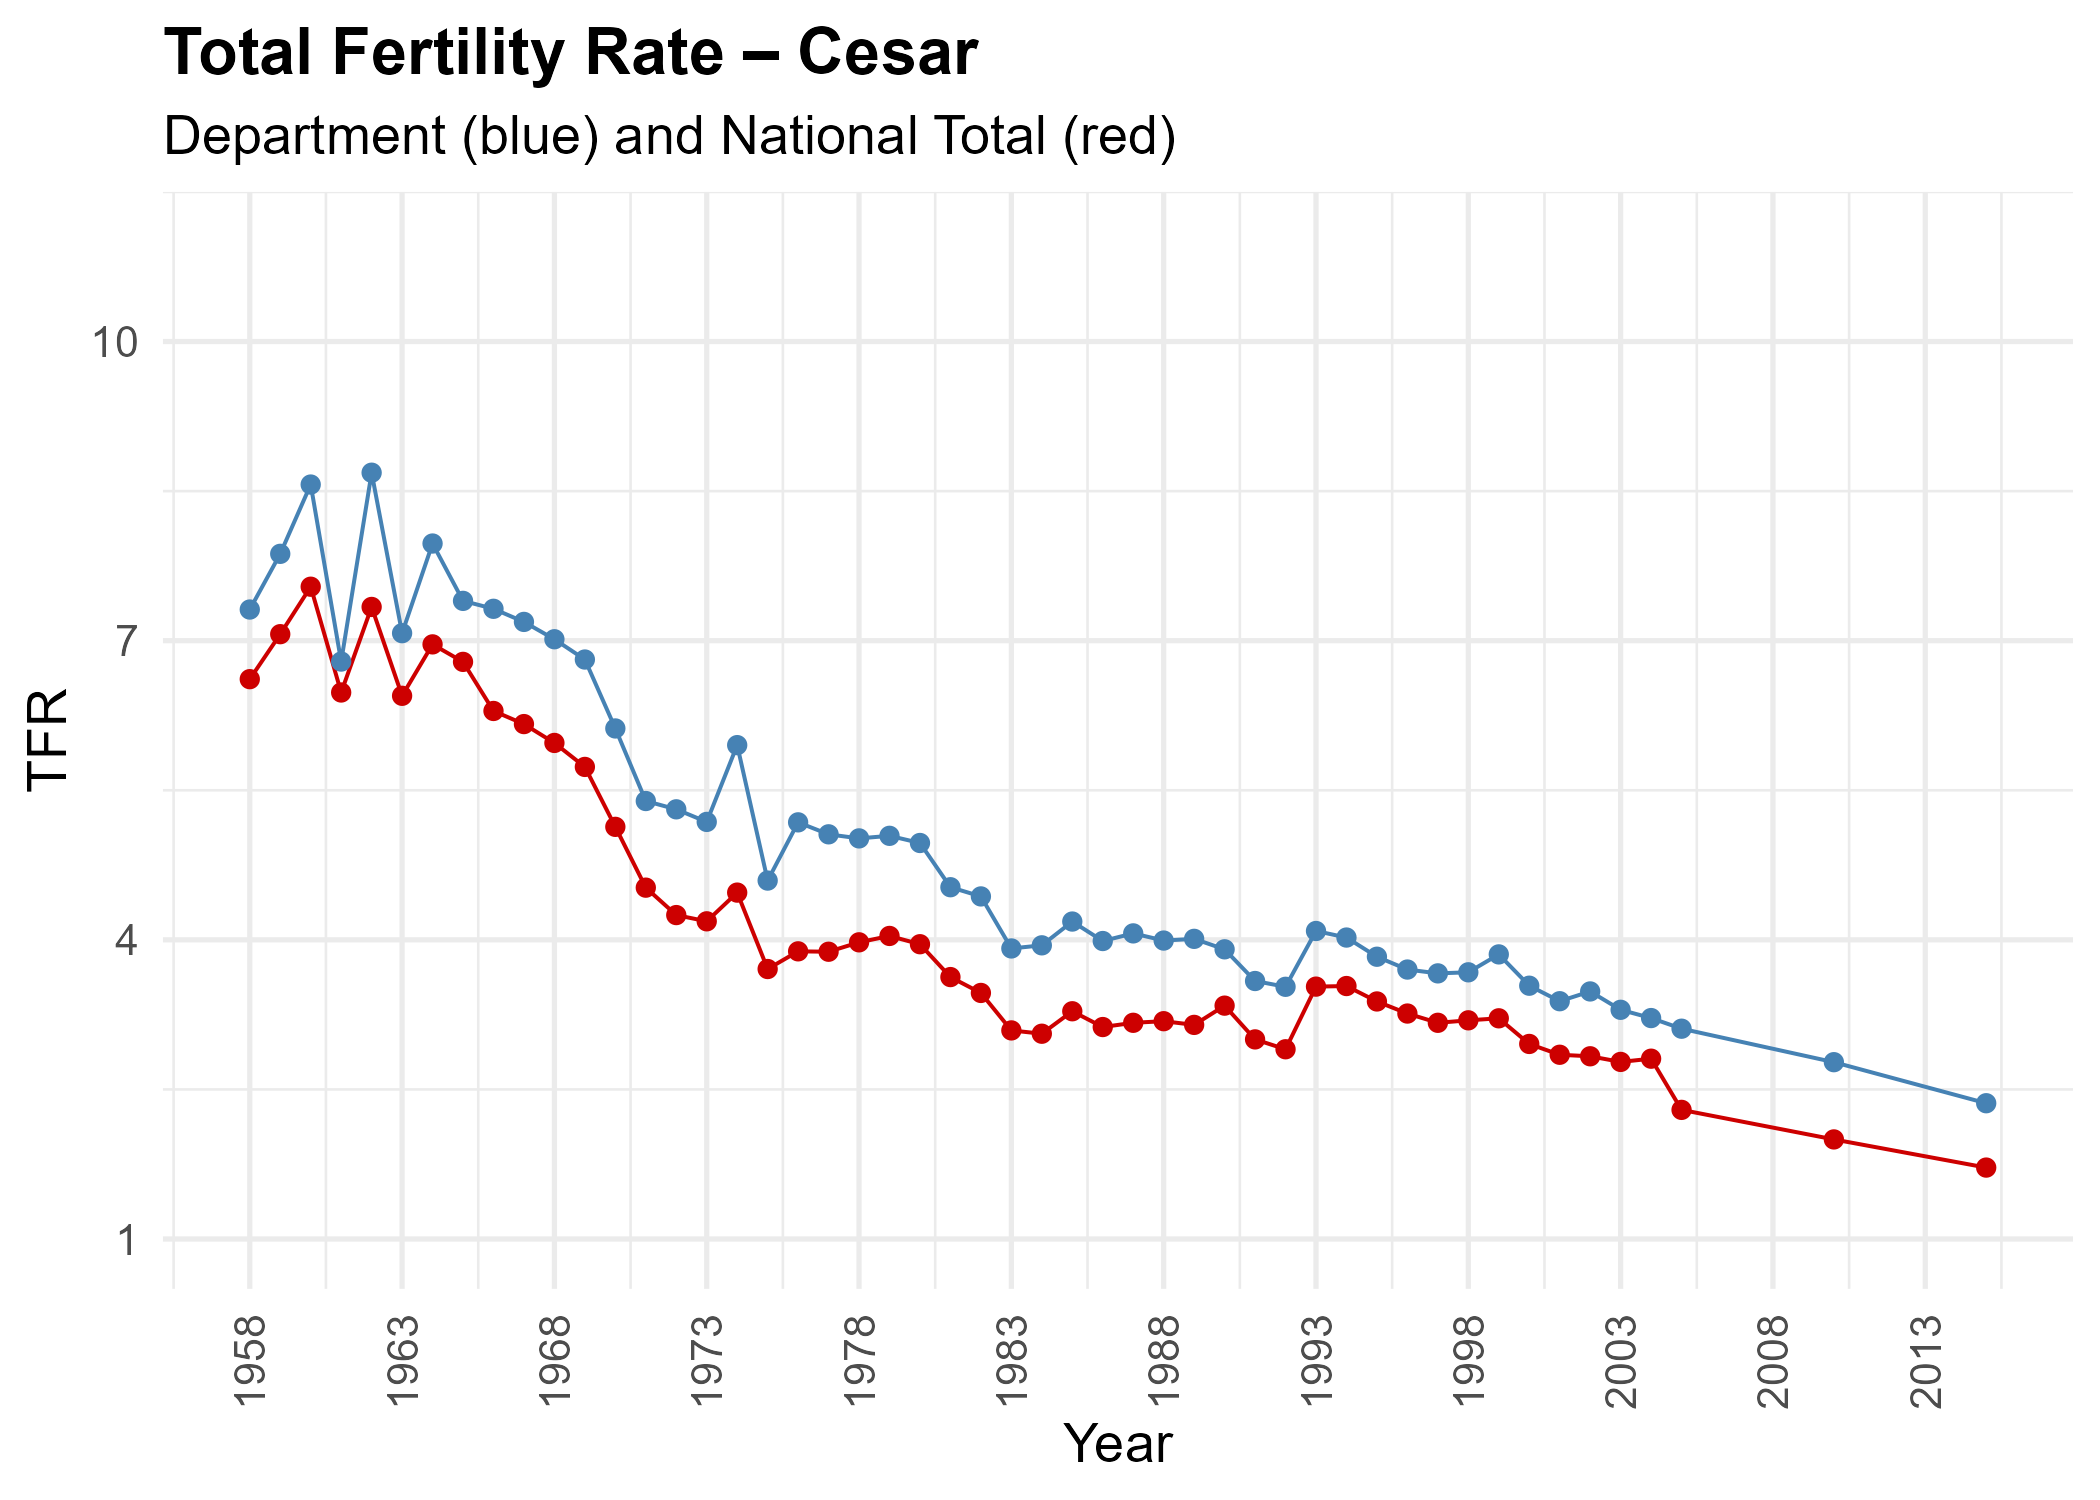
\includegraphics[height=0.78\textheight]{tfr_departamental/TFR_Cesar_vs_National.png}
\end{center}
\end{frame}
\begin{frame}{TGF: Chocó}
\begin{center}
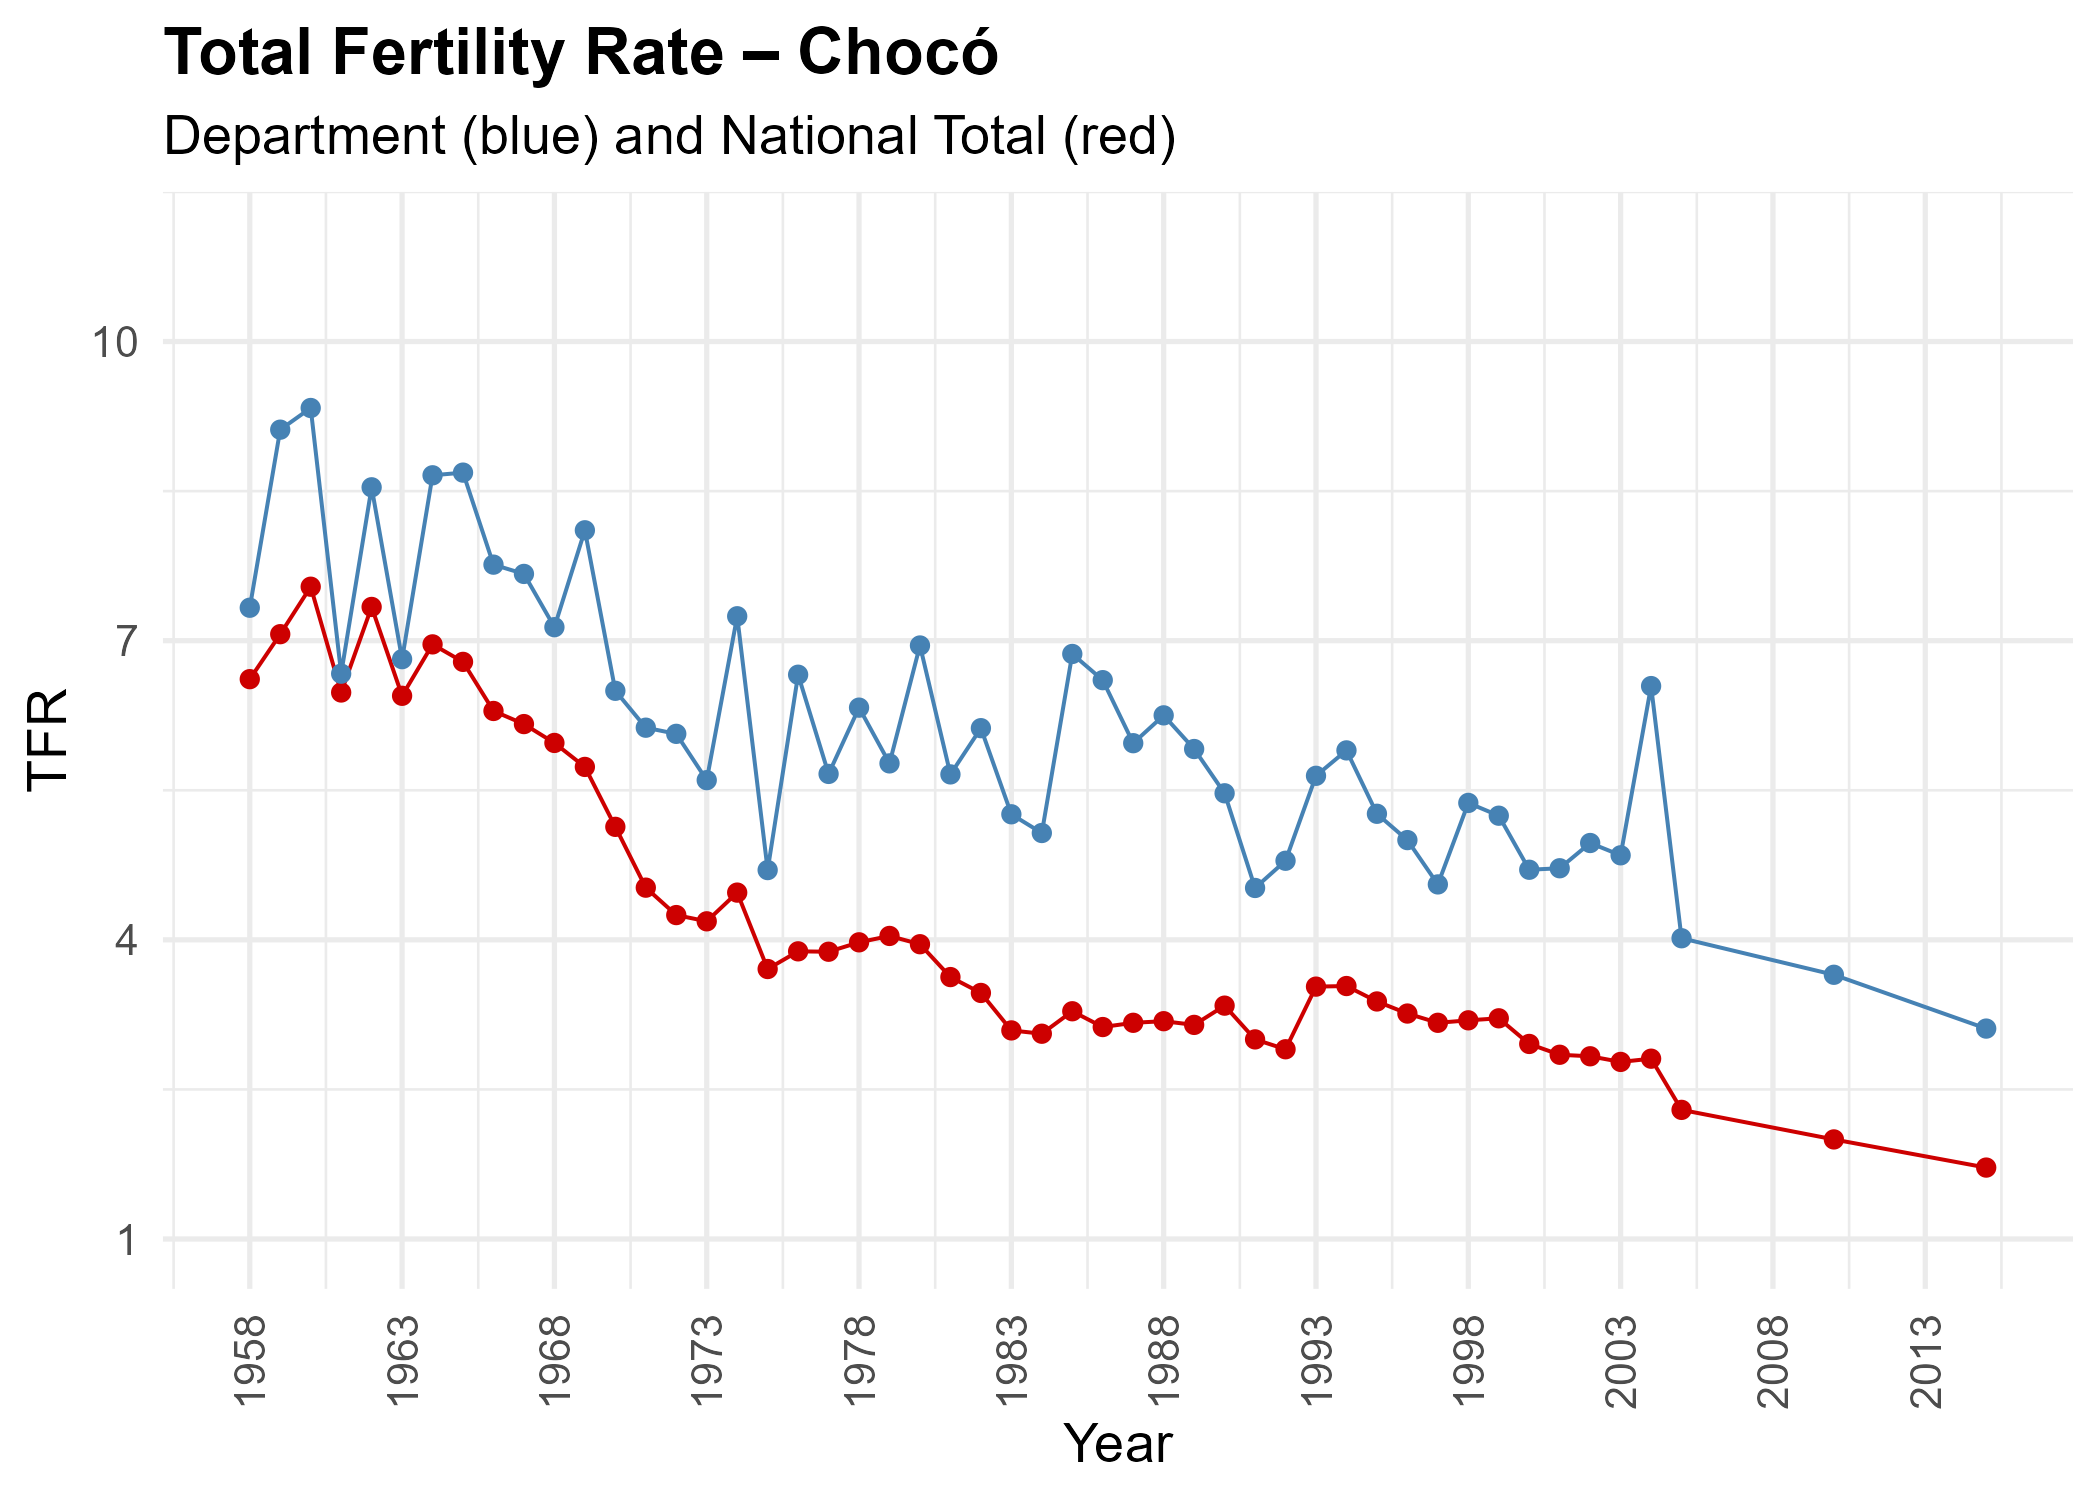
\includegraphics[height=0.78\textheight]{tfr_departamental/TFR_Chocó_vs_National.png}
\end{center}
\end{frame}
\begin{frame}{TGF: Córdoba}
\begin{center}
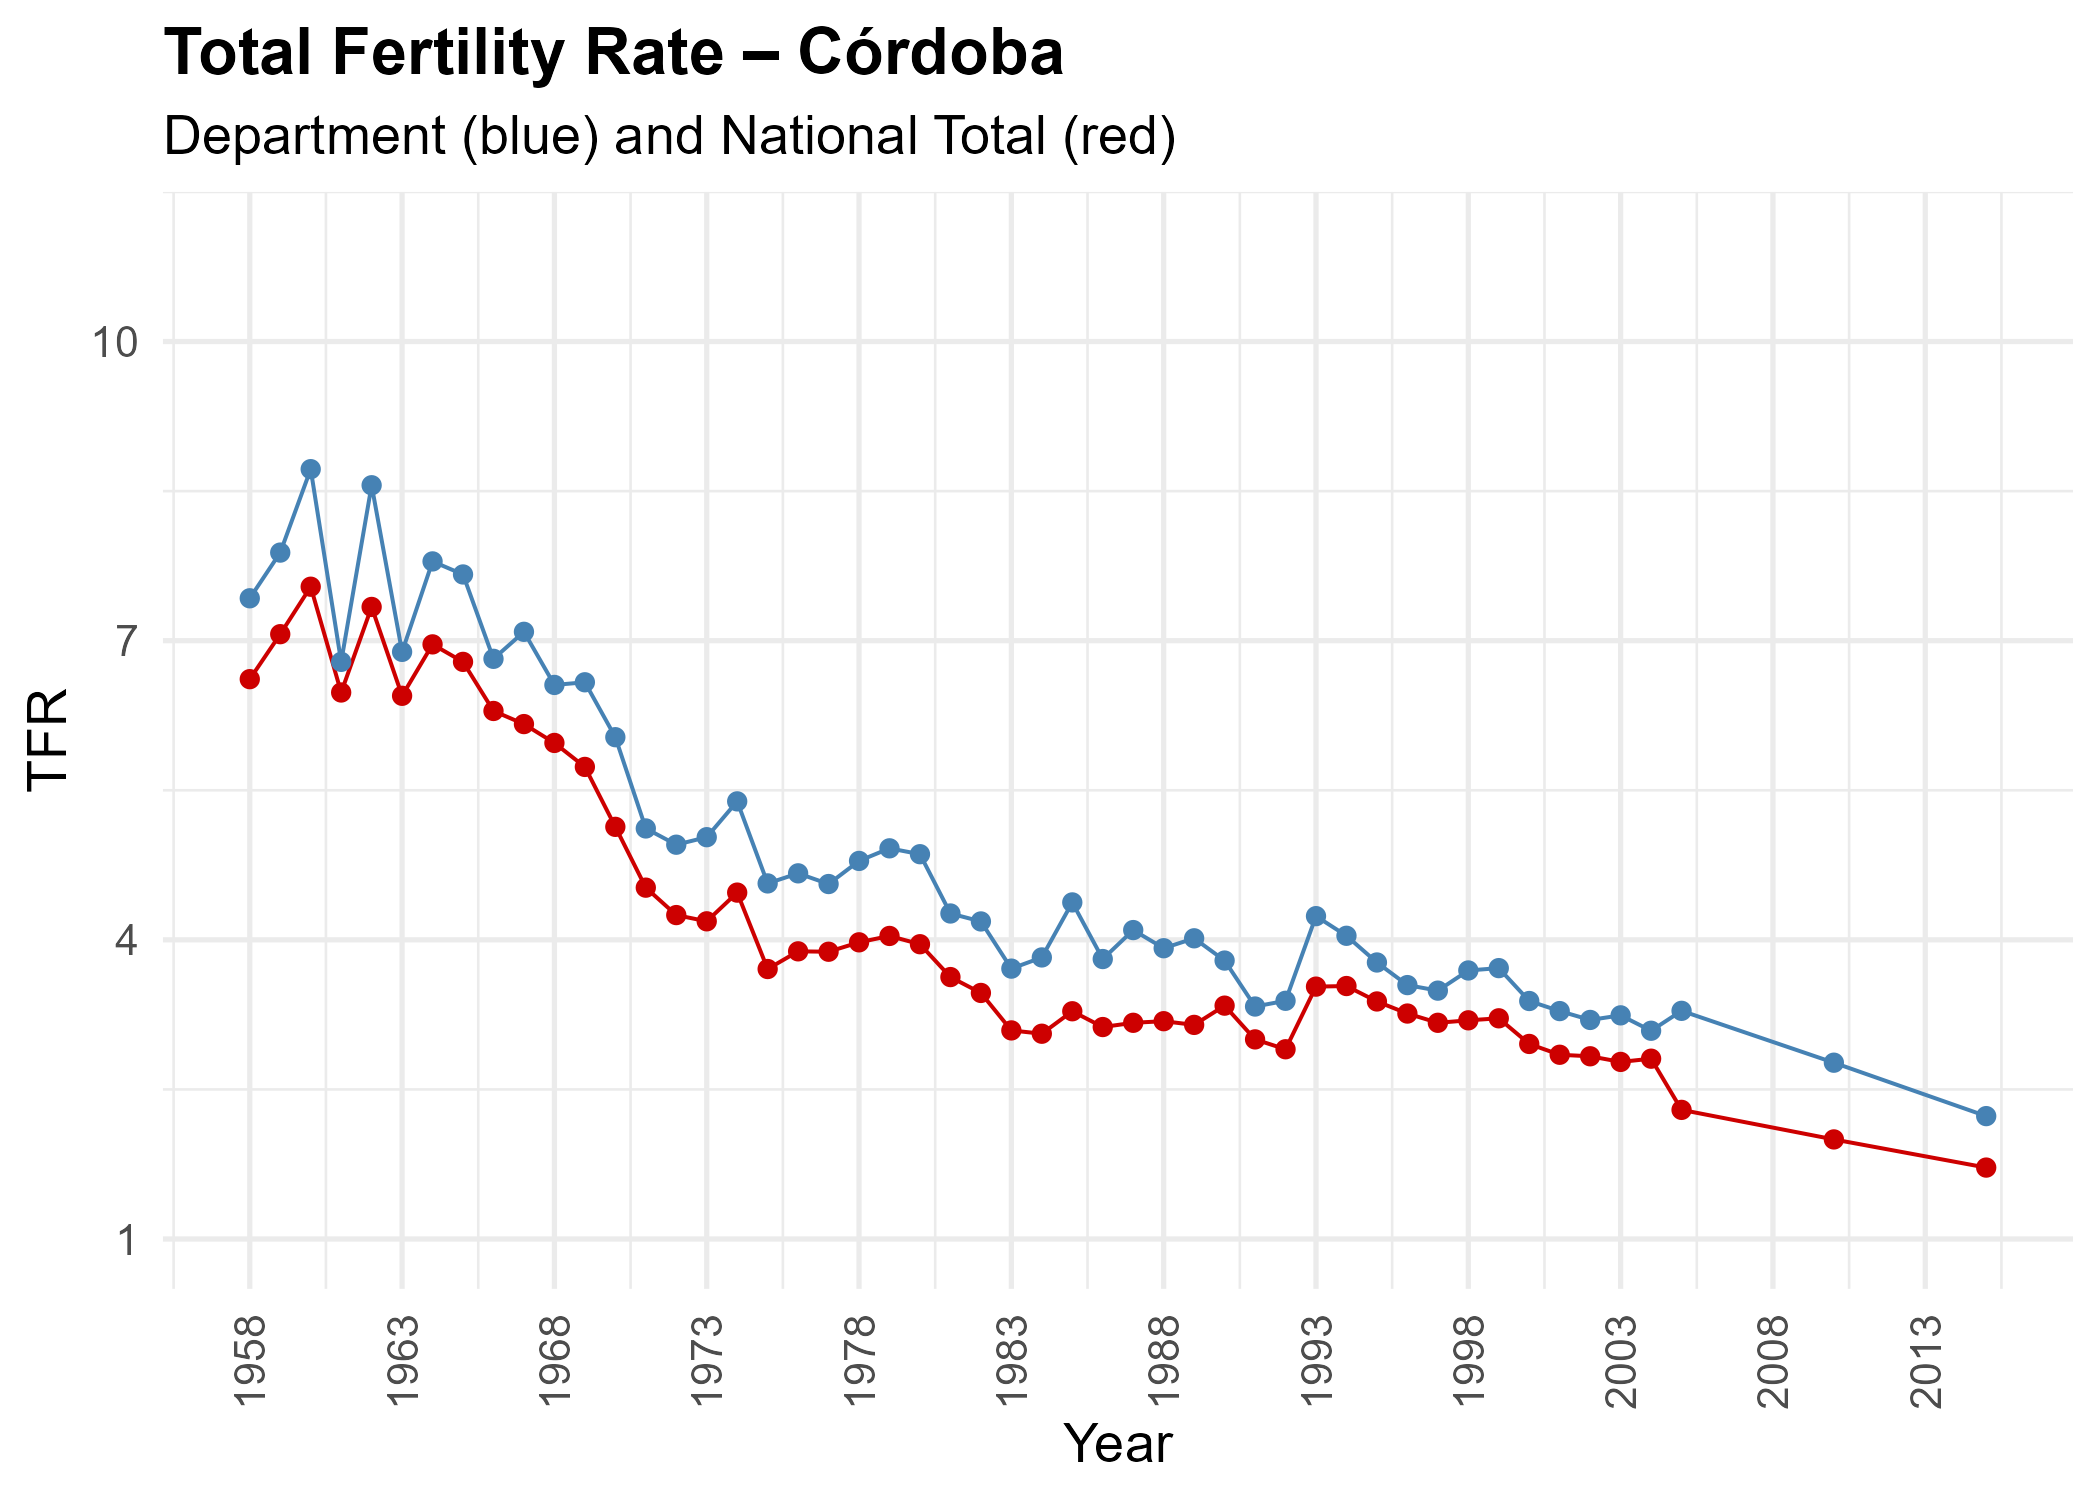
\includegraphics[height=0.78\textheight]{tfr_departamental/TFR_Córdoba_vs_National.png}
\end{center}
\end{frame}
\begin{frame}{TGF: Huila}
\begin{center}
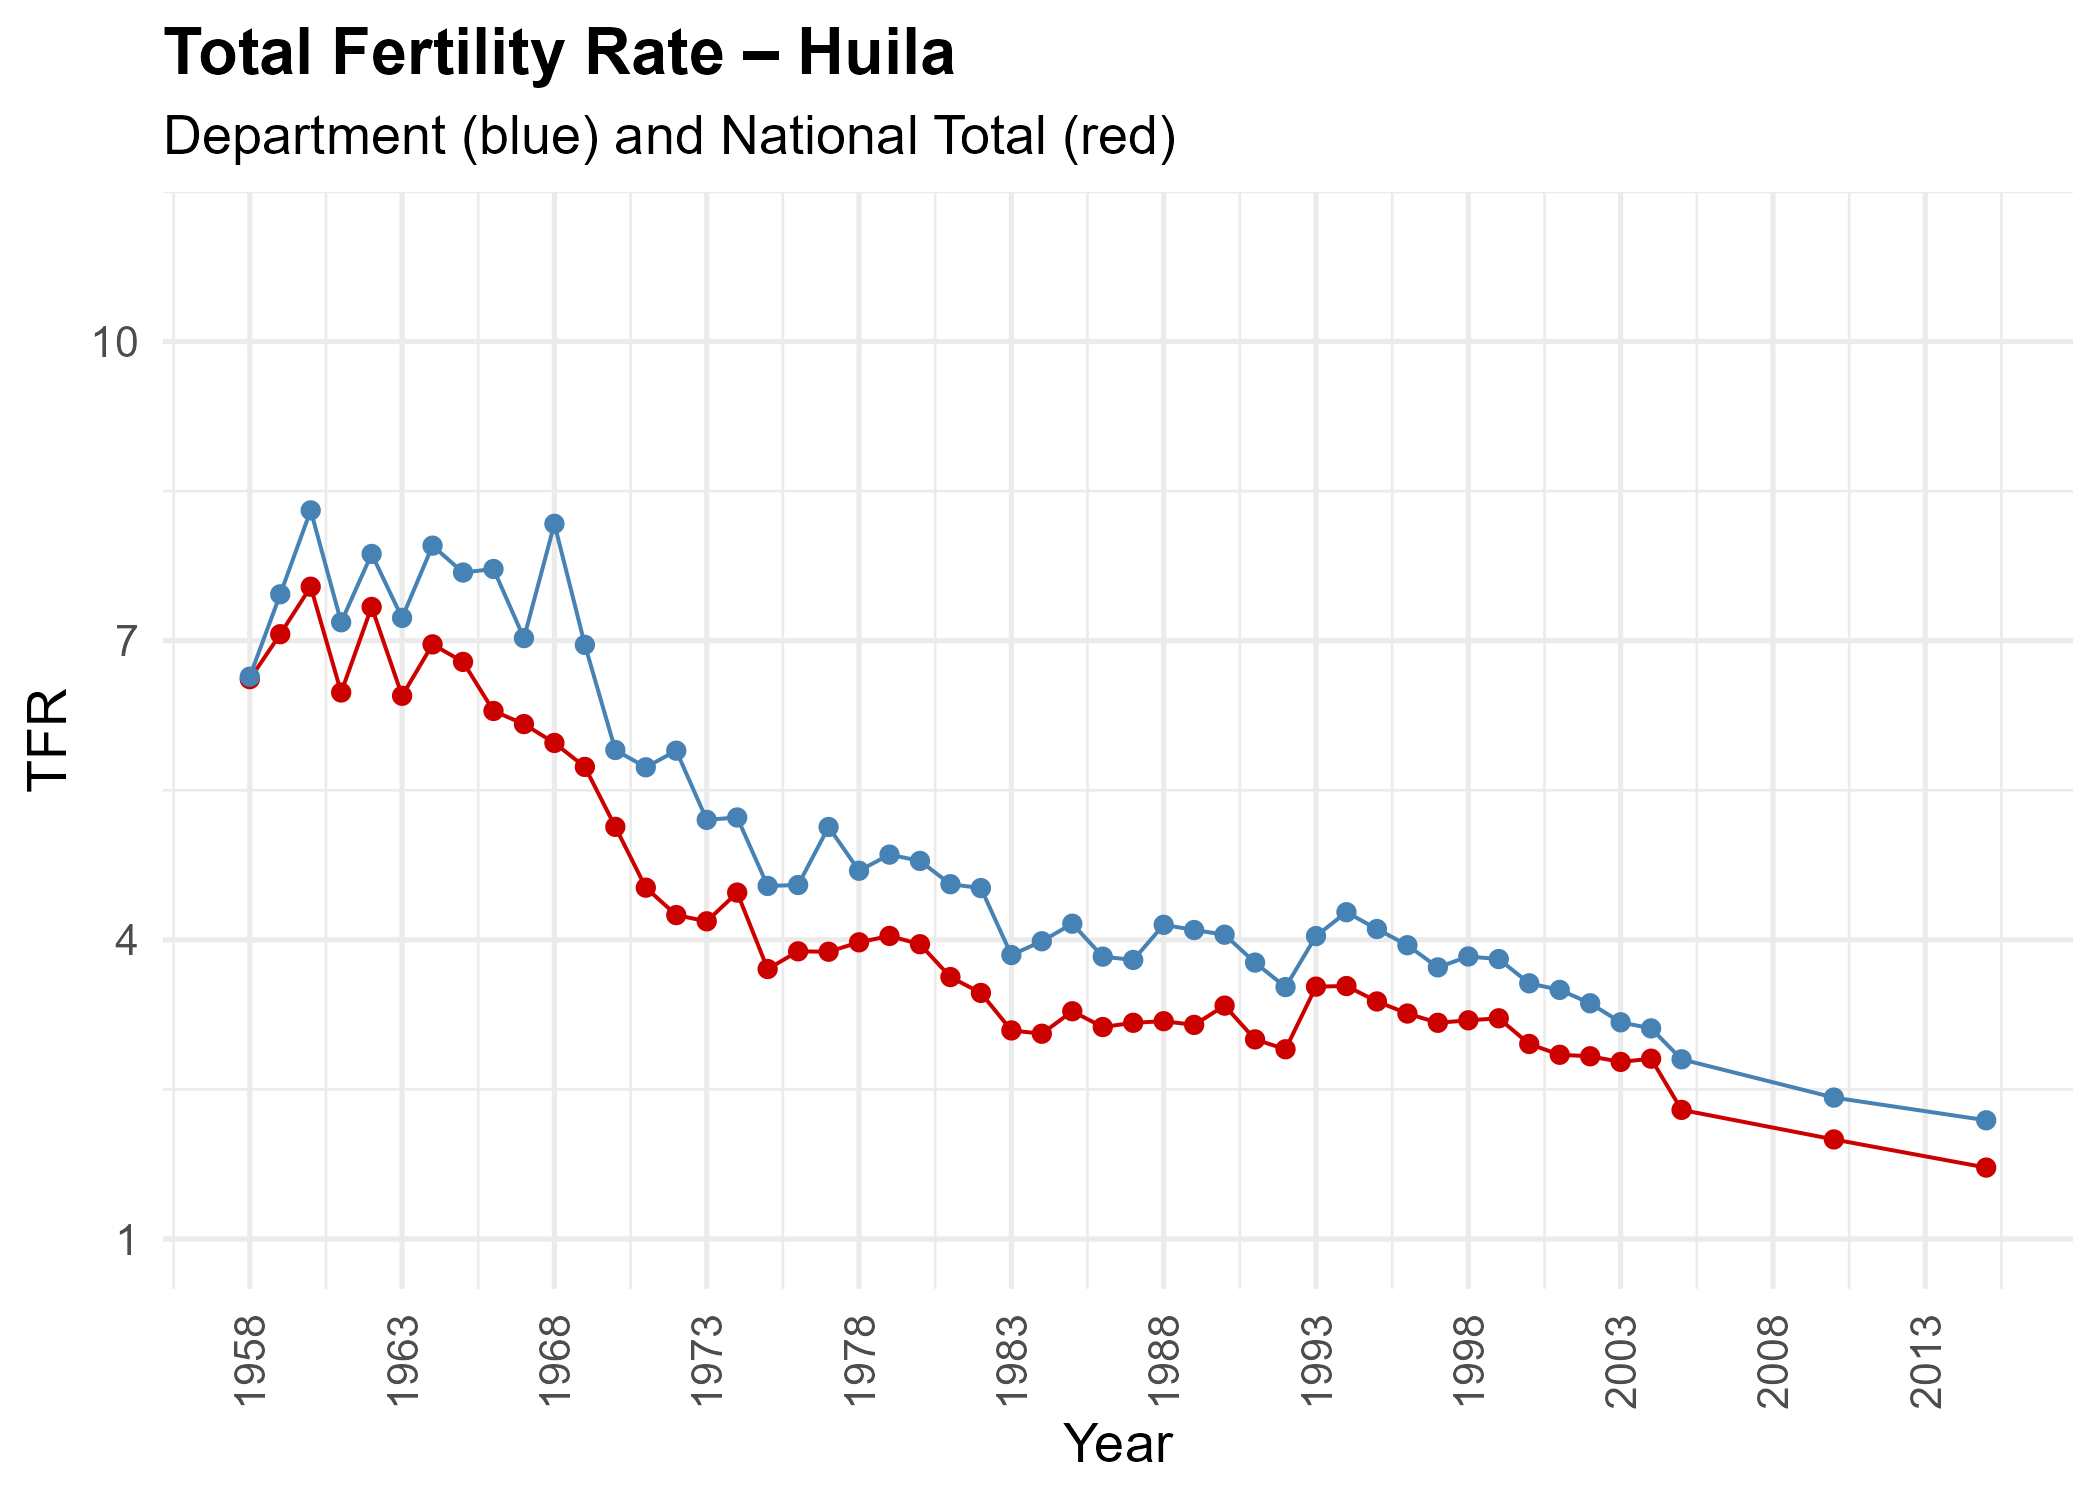
\includegraphics[height=0.78\textheight]{tfr_departamental/TFR_Huila_vs_National.png}
\end{center}
\end{frame}
\begin{frame}{TGF: La Guajira}
\begin{center}
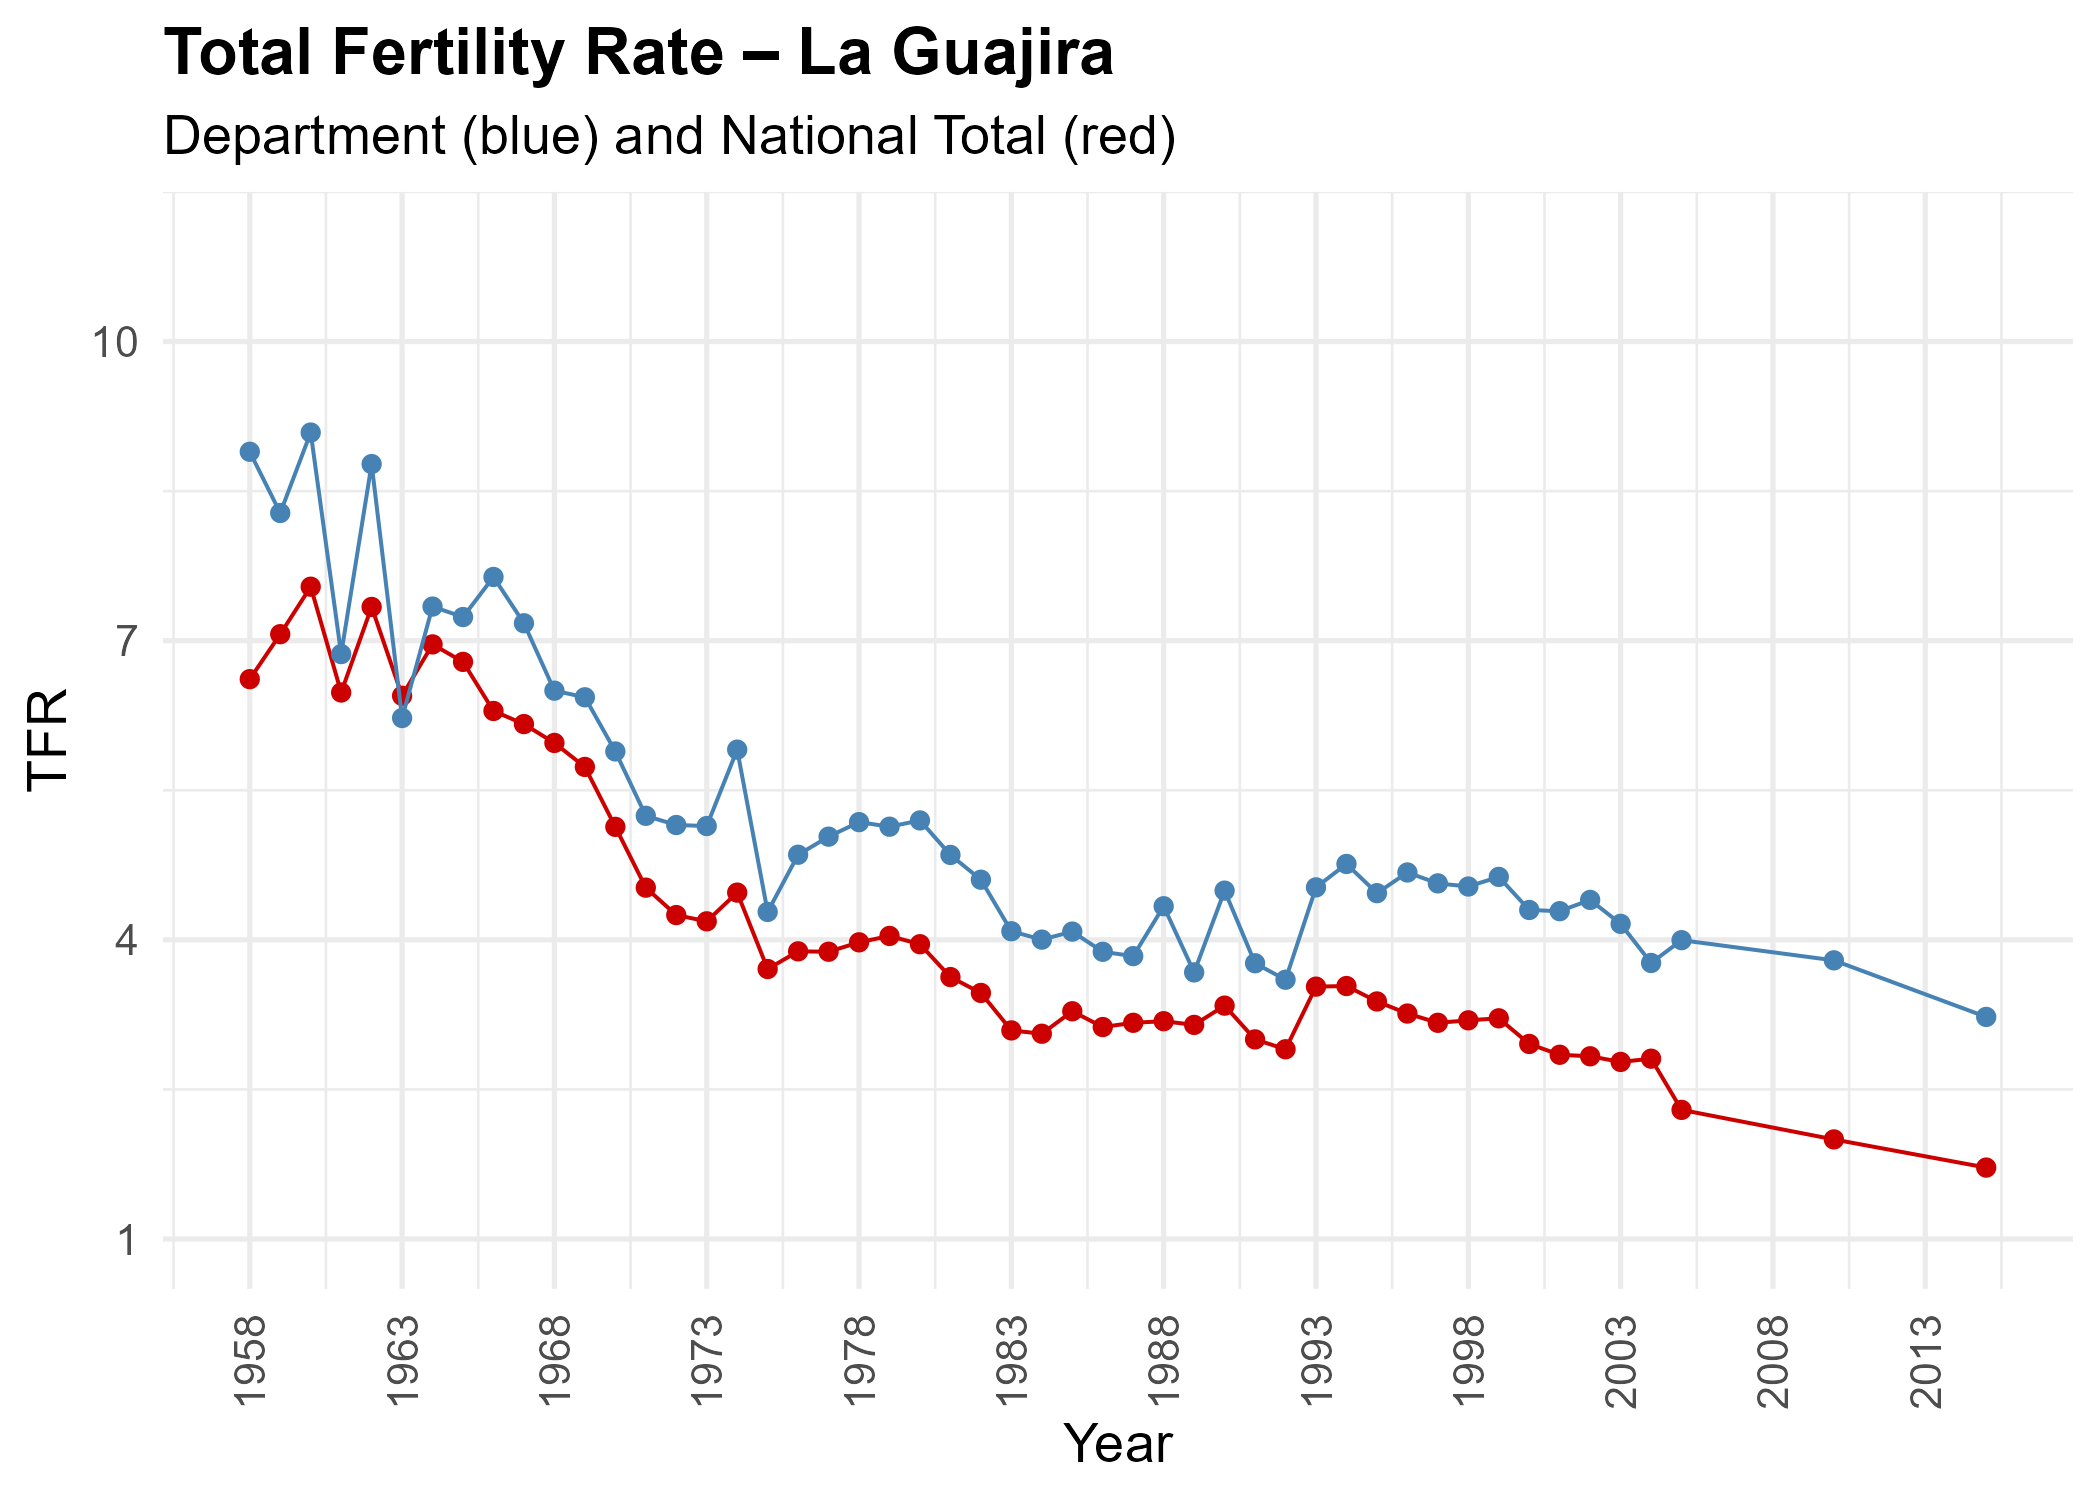
\includegraphics[height=0.78\textheight]{tfr_departamental/TFR_La Guajira_vs_National.png}
\end{center}
\end{frame}
\begin{frame}{TGF: Meta}
\begin{center}
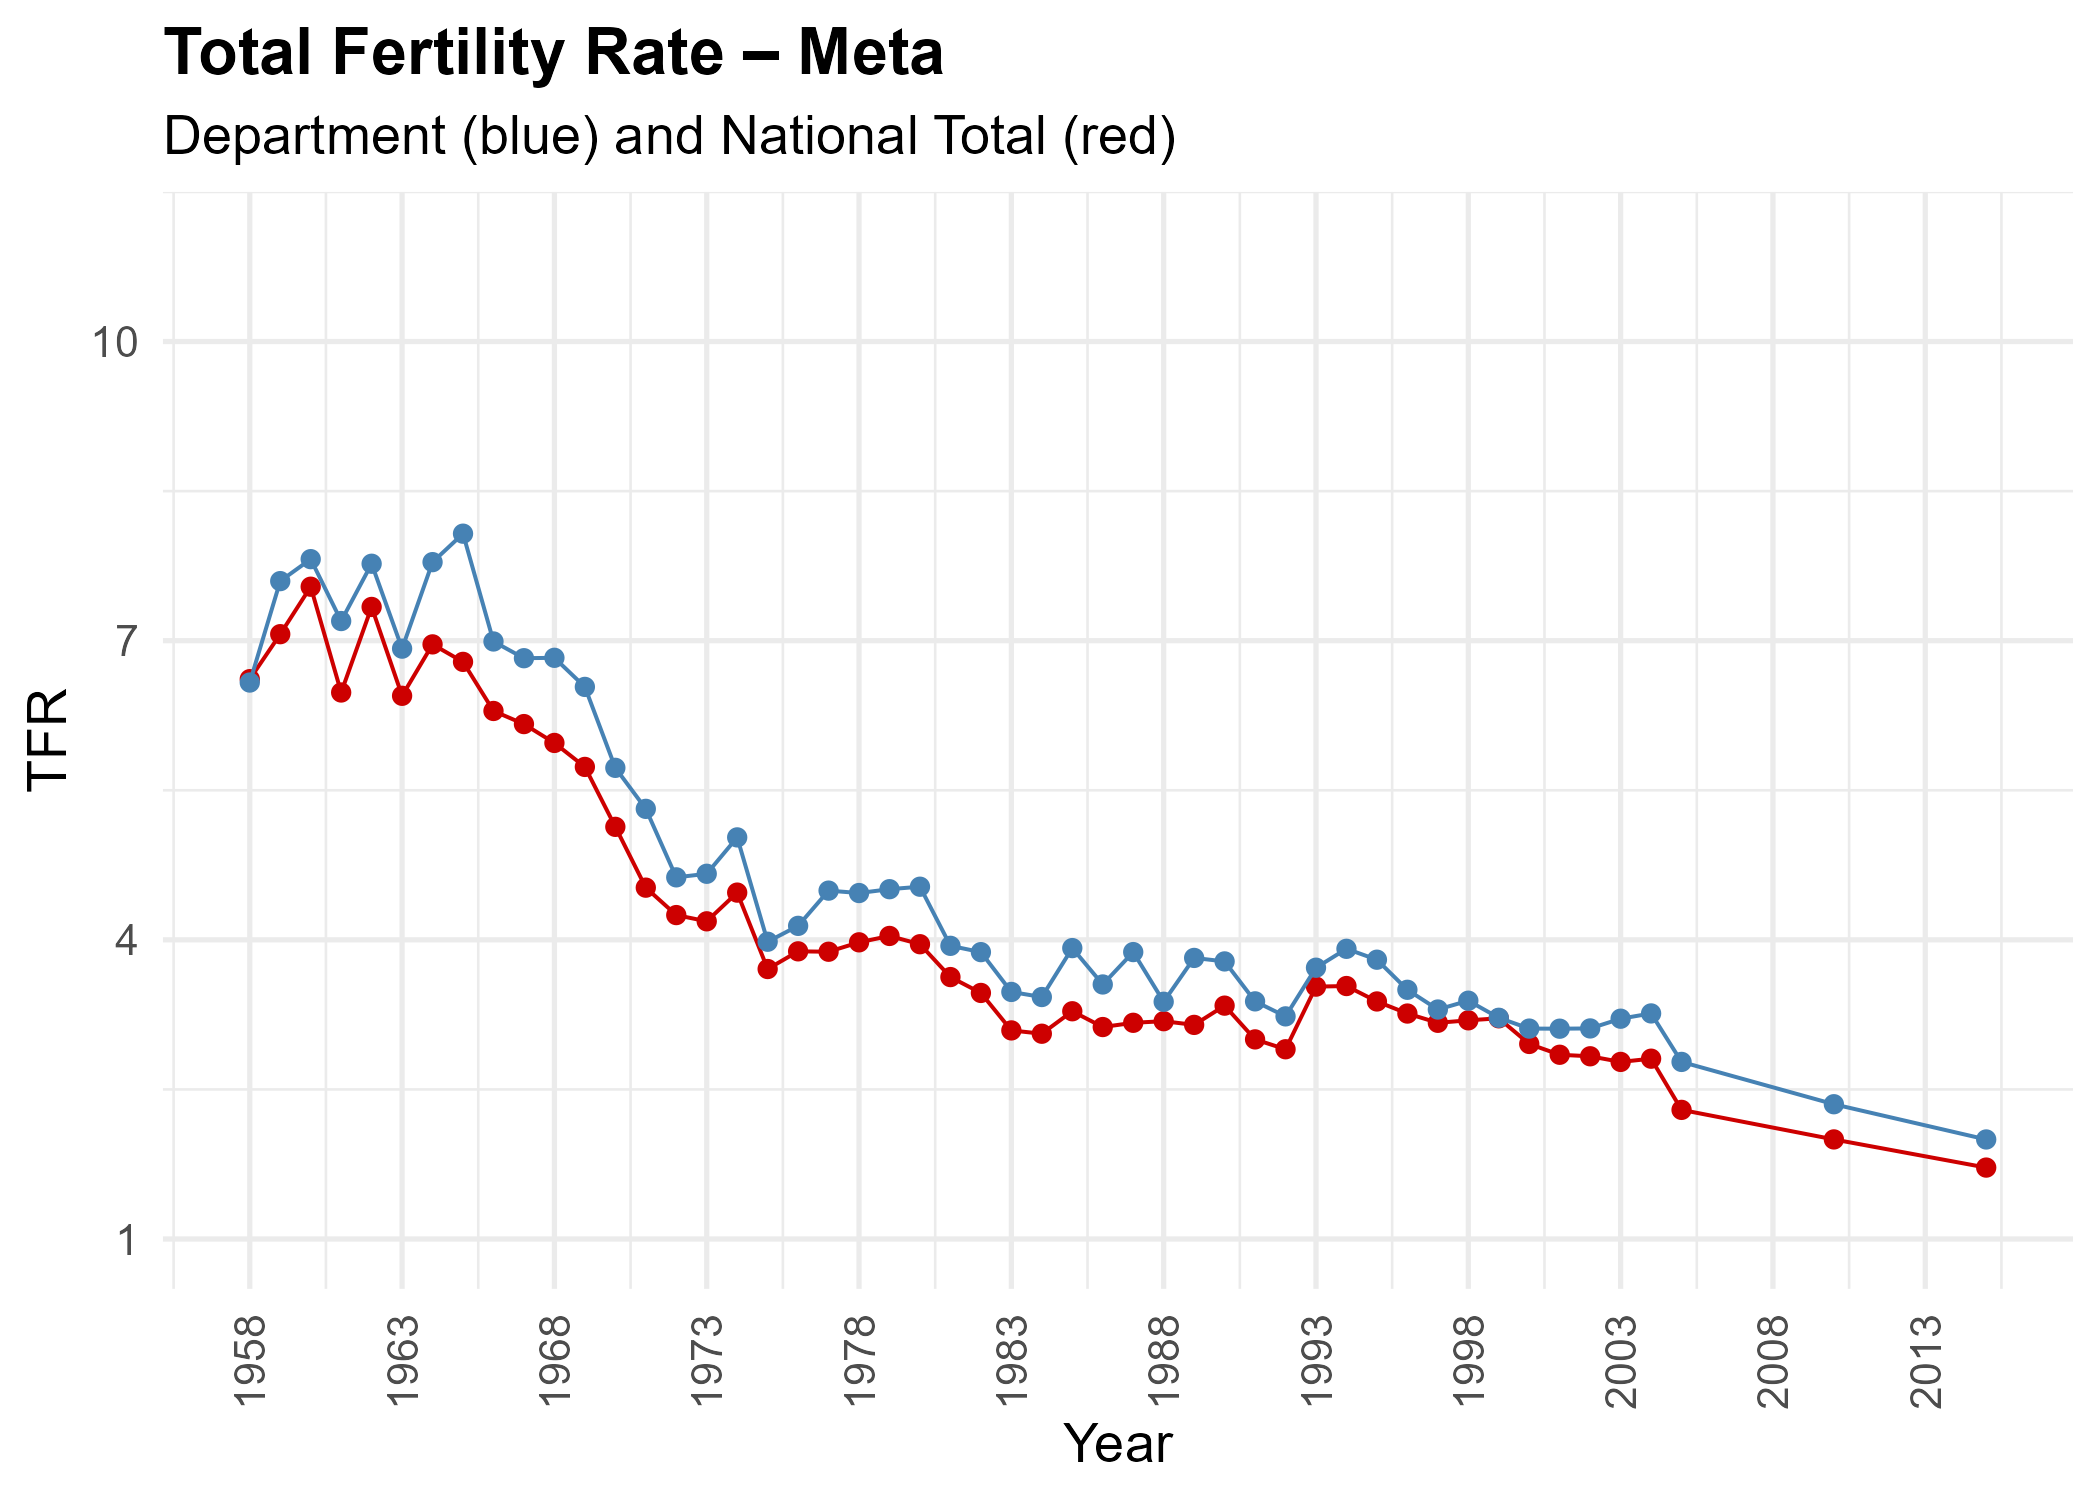
\includegraphics[height=0.78\textheight]{tfr_departamental/TFR_Meta_vs_National.png}
\end{center}
\end{frame}
\begin{frame}{TGF: Nariño}
\begin{center}
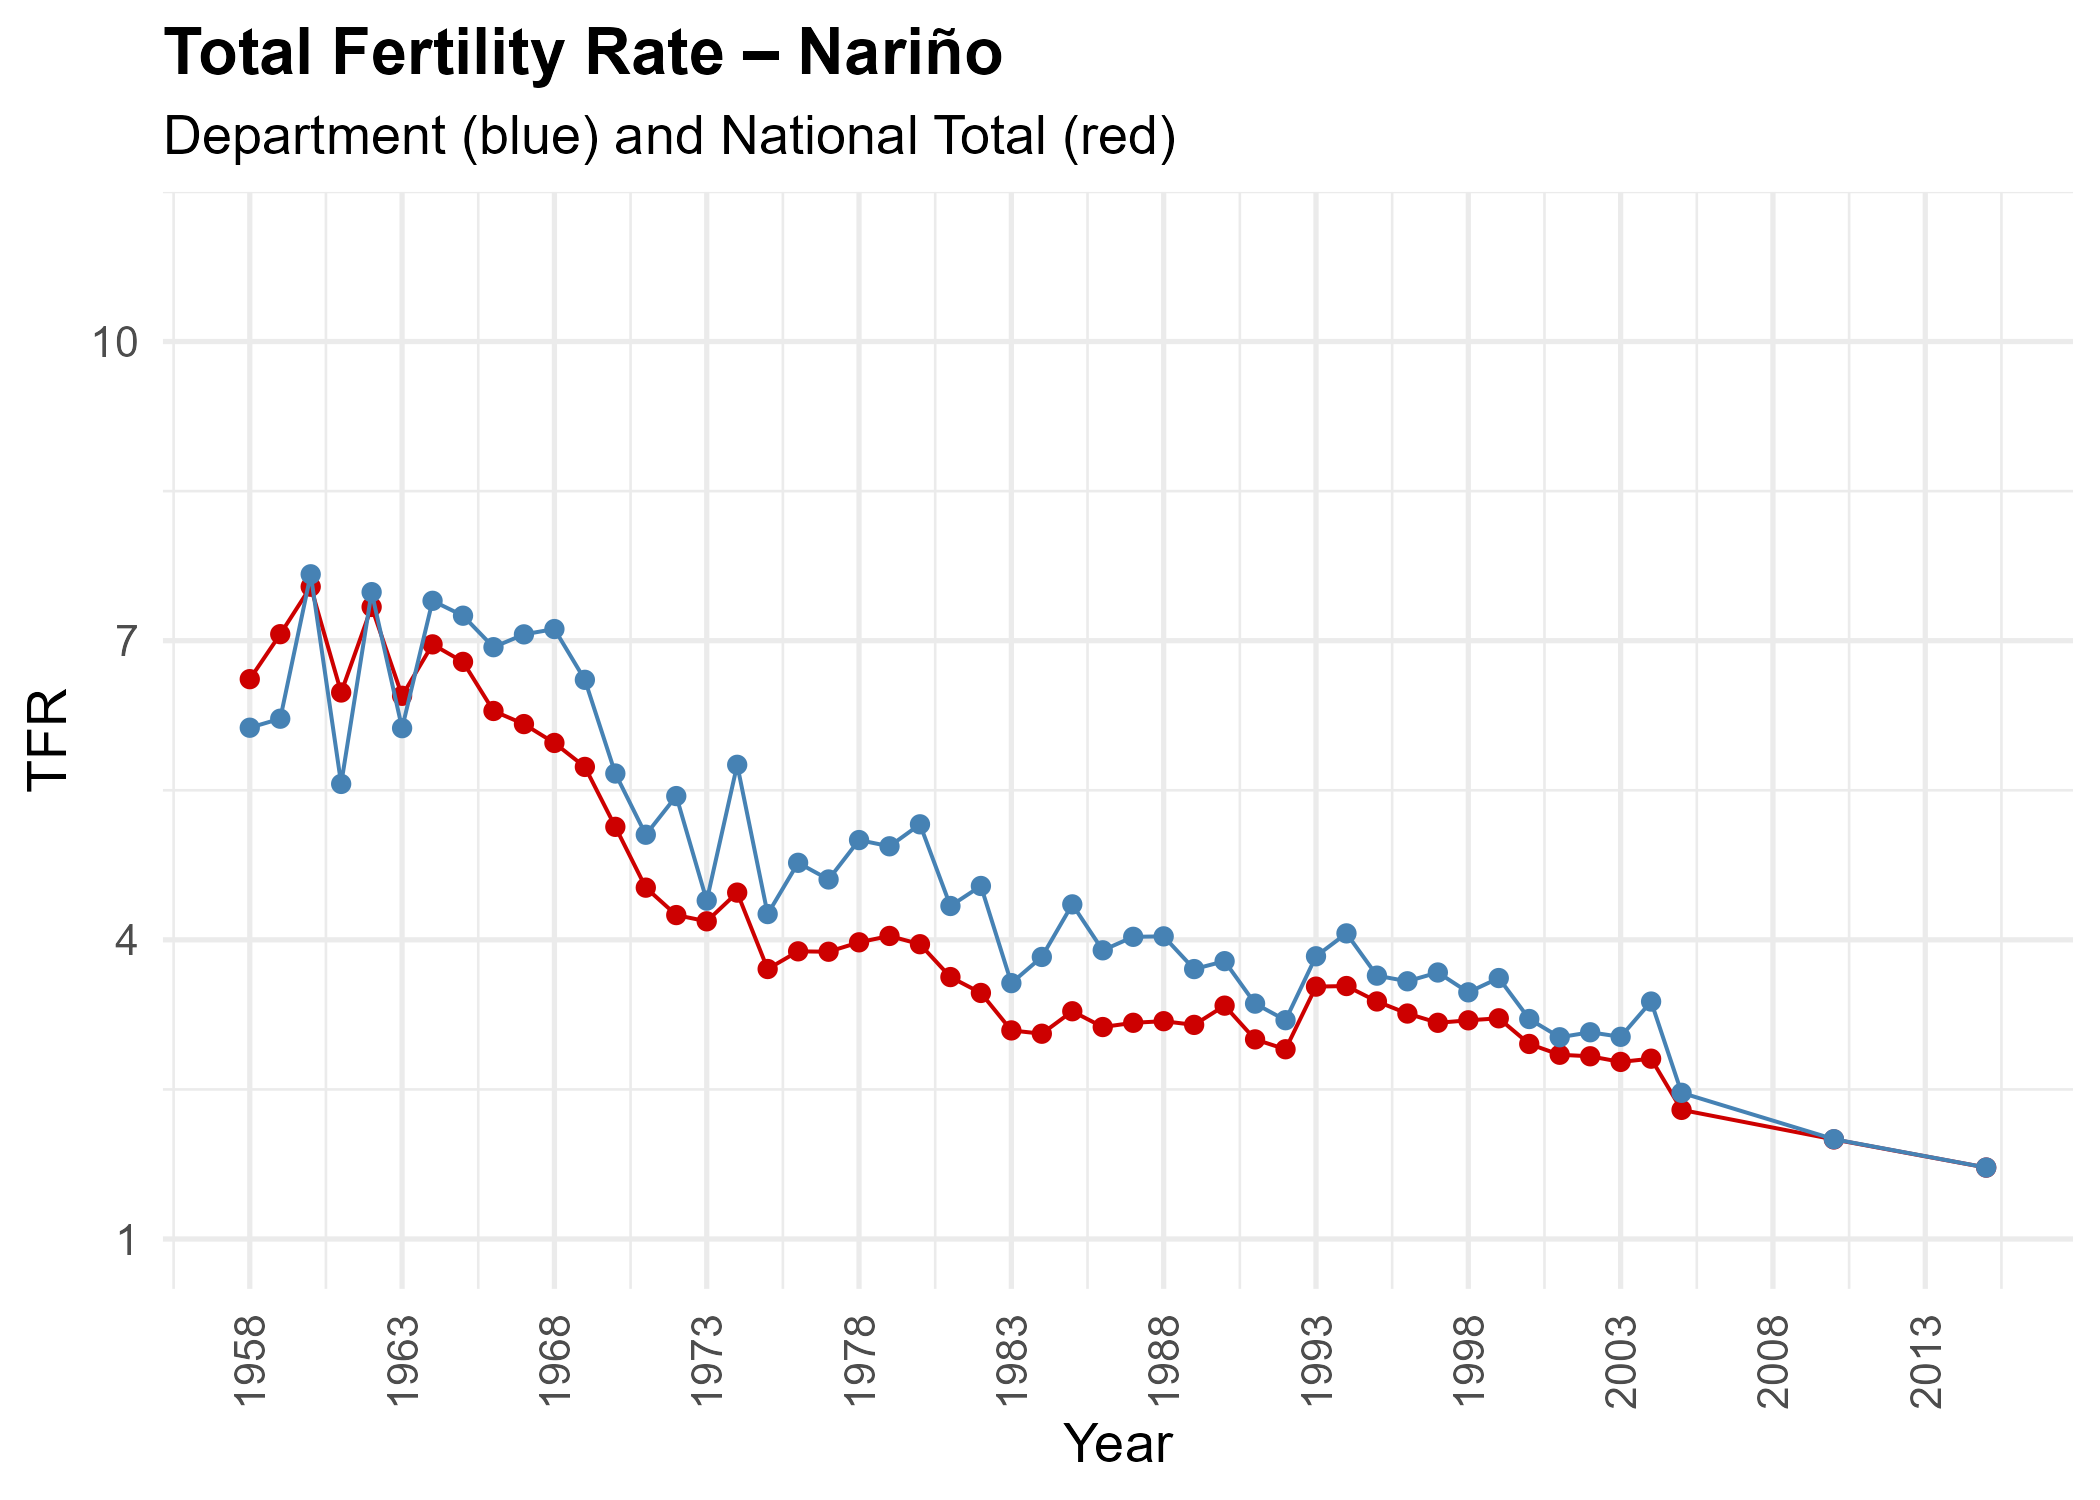
\includegraphics[height=0.78\textheight]{tfr_departamental/TFR_Nariño_vs_National.png}
\end{center}
\end{frame}
\begin{frame}{TGF: Putumayo}
\begin{center}
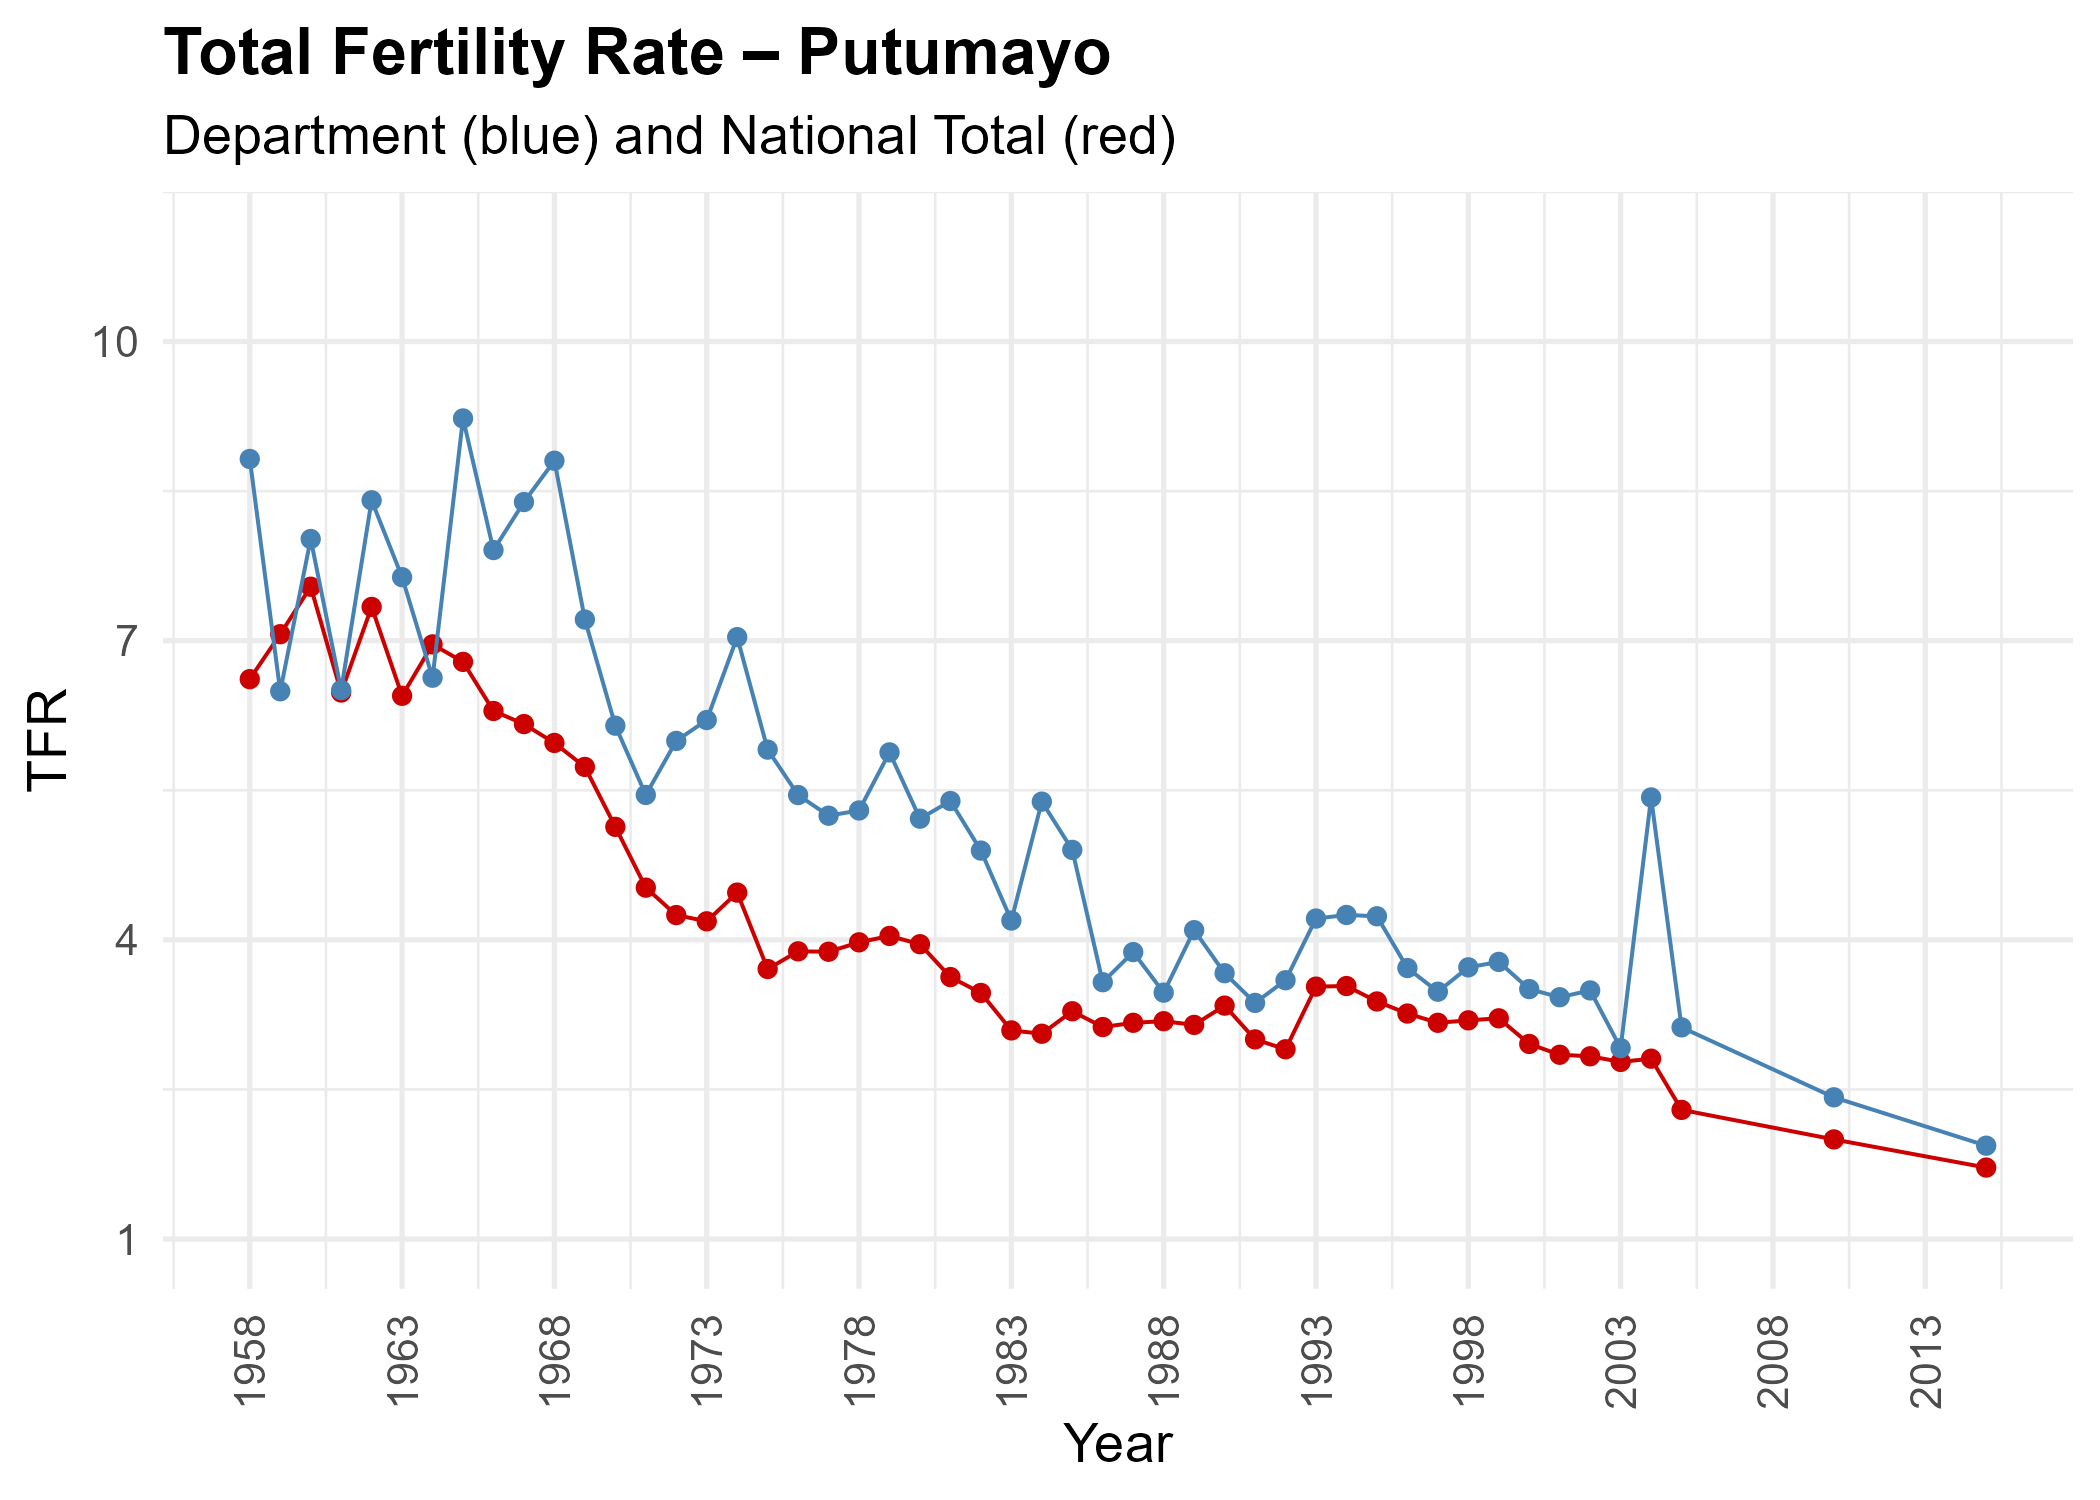
\includegraphics[height=0.78\textheight]{tfr_departamental/TFR_Putumayo_vs_National.png}
\end{center}
\end{frame}
\begin{frame}{TGF: San Andrés}
\begin{center}
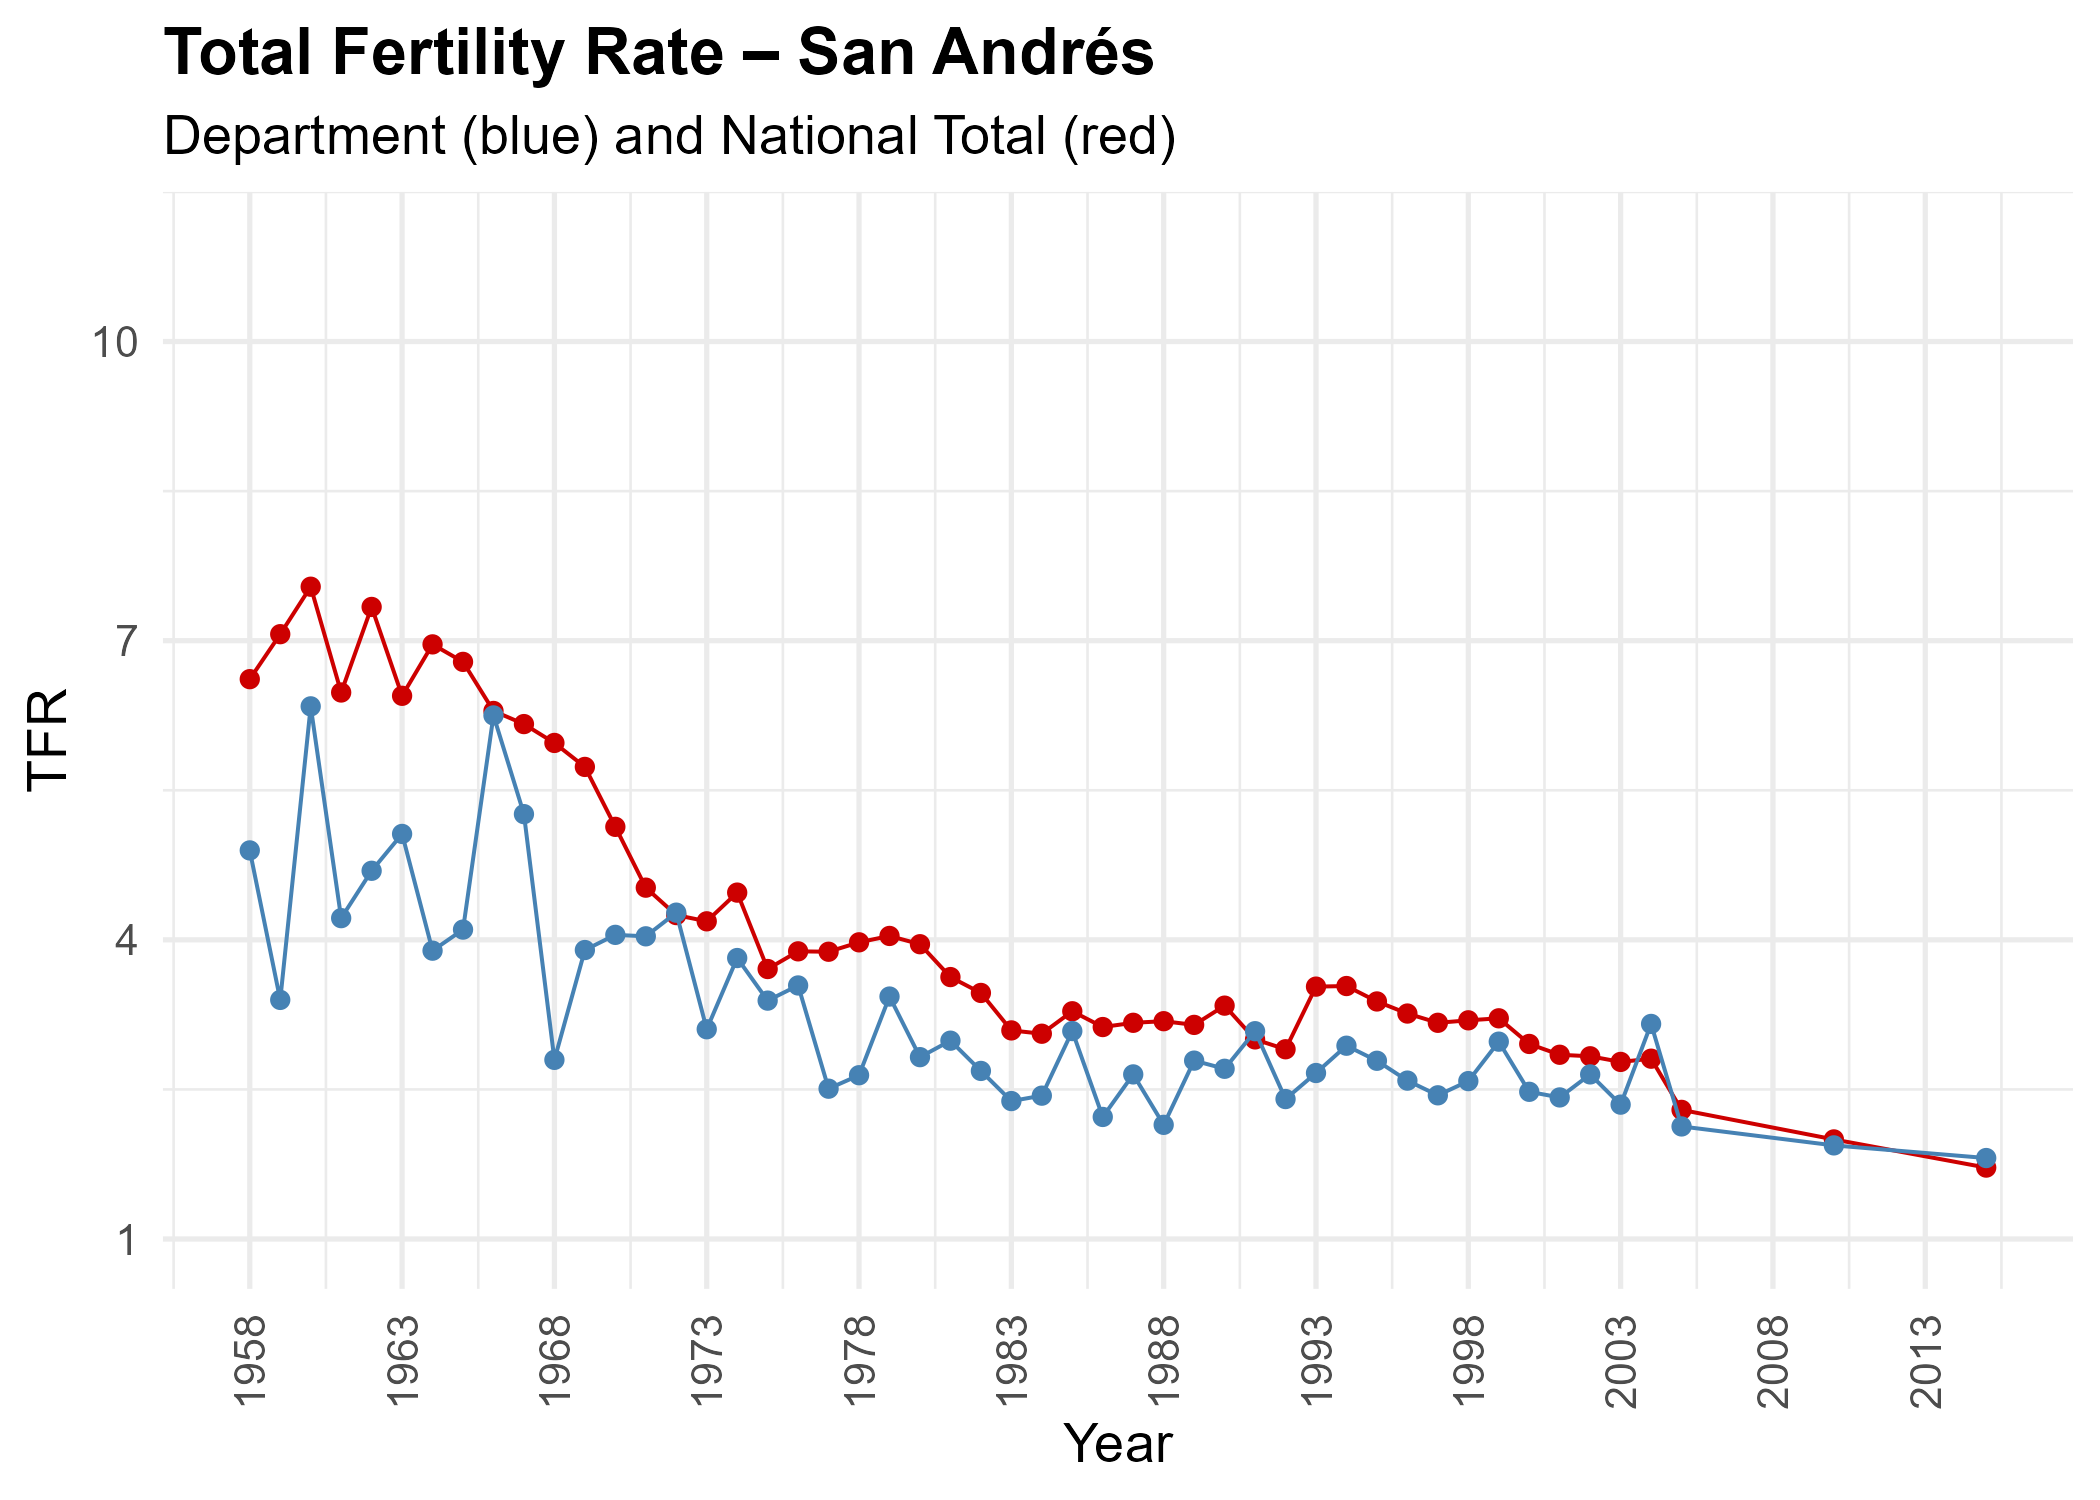
\includegraphics[height=0.78\textheight]{tfr_departamental/TFR_San Andrés_vs_National.png}
\end{center}
\end{frame}
\begin{frame}{TGF: Santander}
\begin{center}
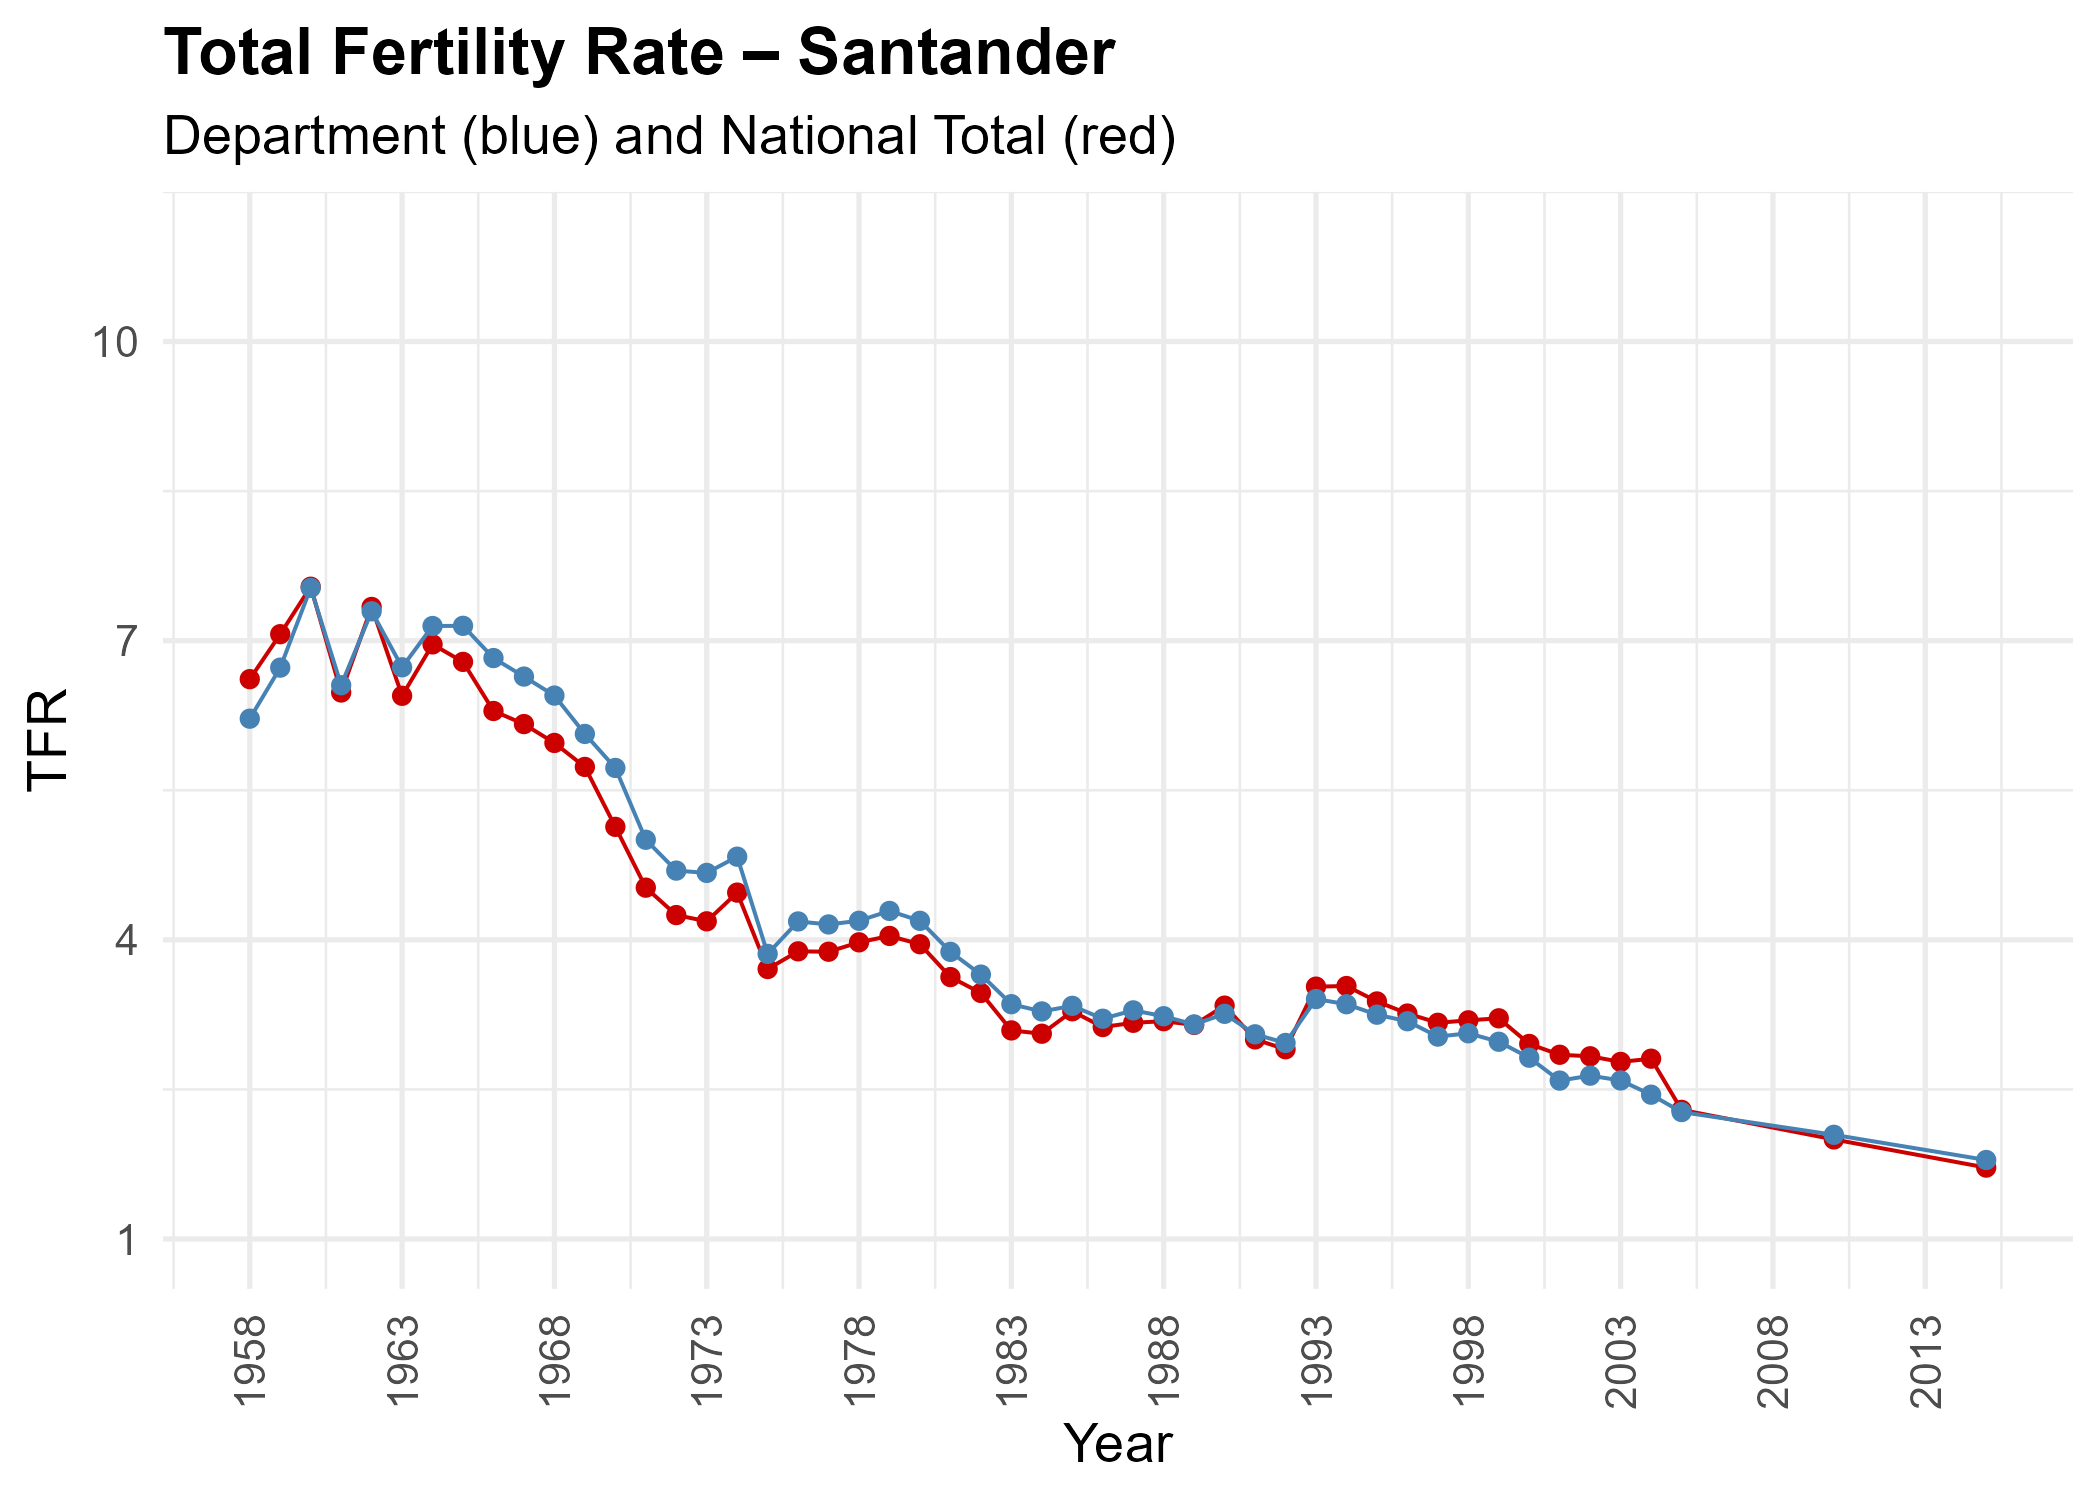
\includegraphics[height=0.78\textheight]{tfr_departamental/TFR_Santander_vs_National.png}
\end{center}
\end{frame}
\begin{frame}{TGF: Tolima}
\begin{center}
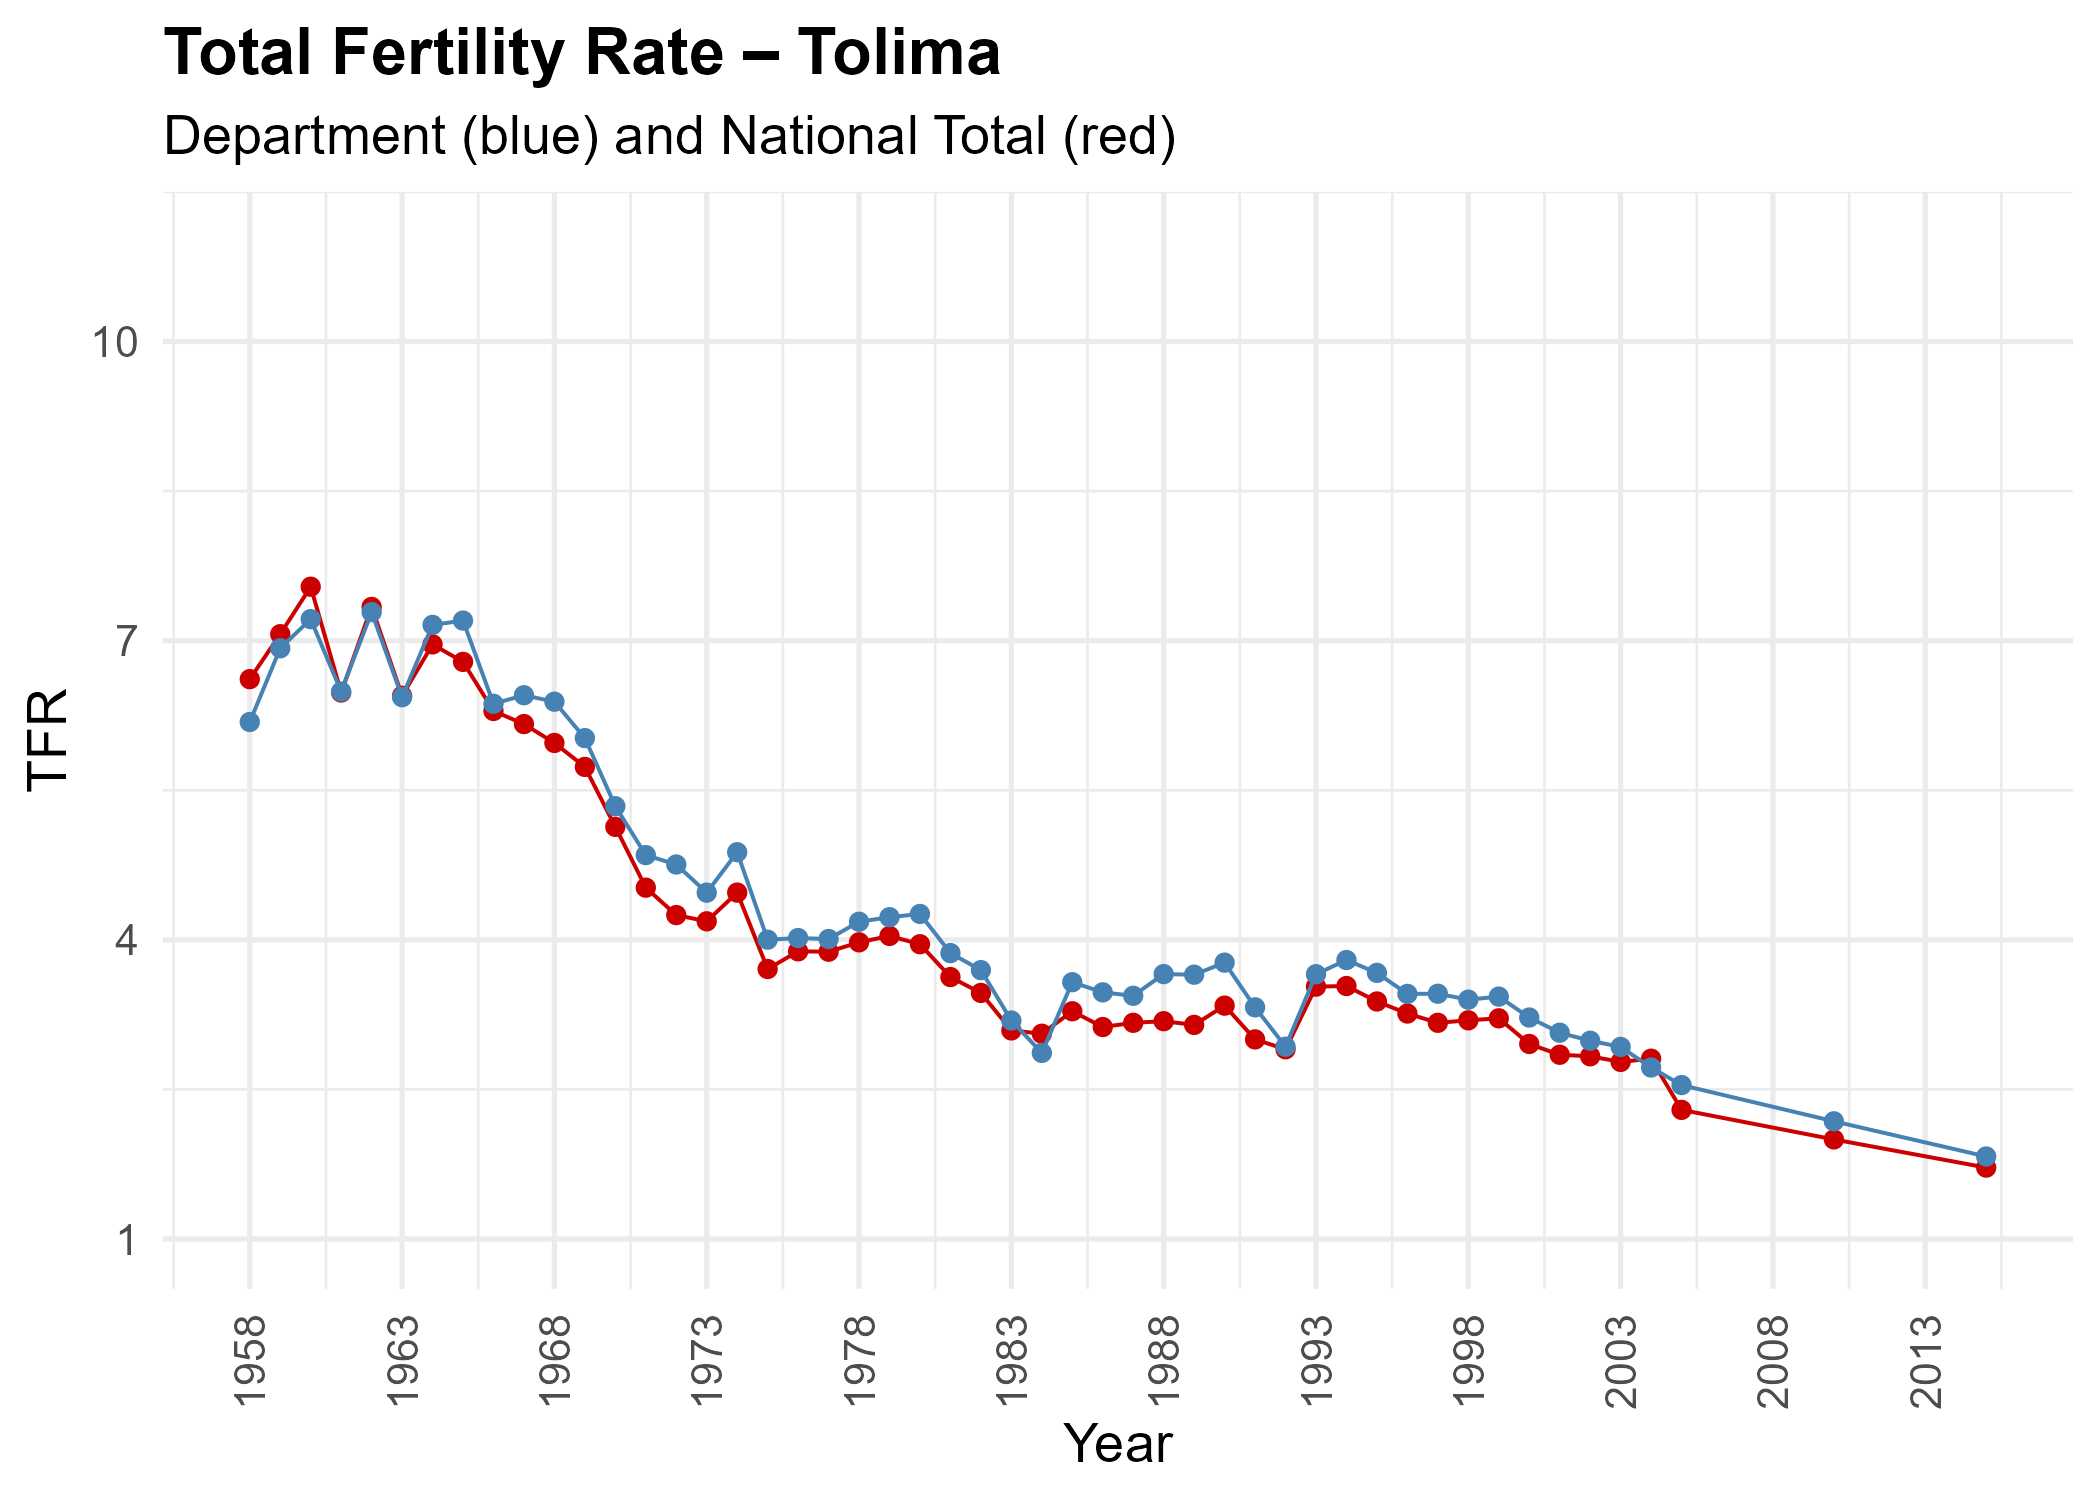
\includegraphics[height=0.78\textheight]{tfr_departamental/TFR_Tolima_vs_National.png}
\end{center}
\end{frame}
\begin{frame}{TGF: Valle del Cauca}
\begin{center}
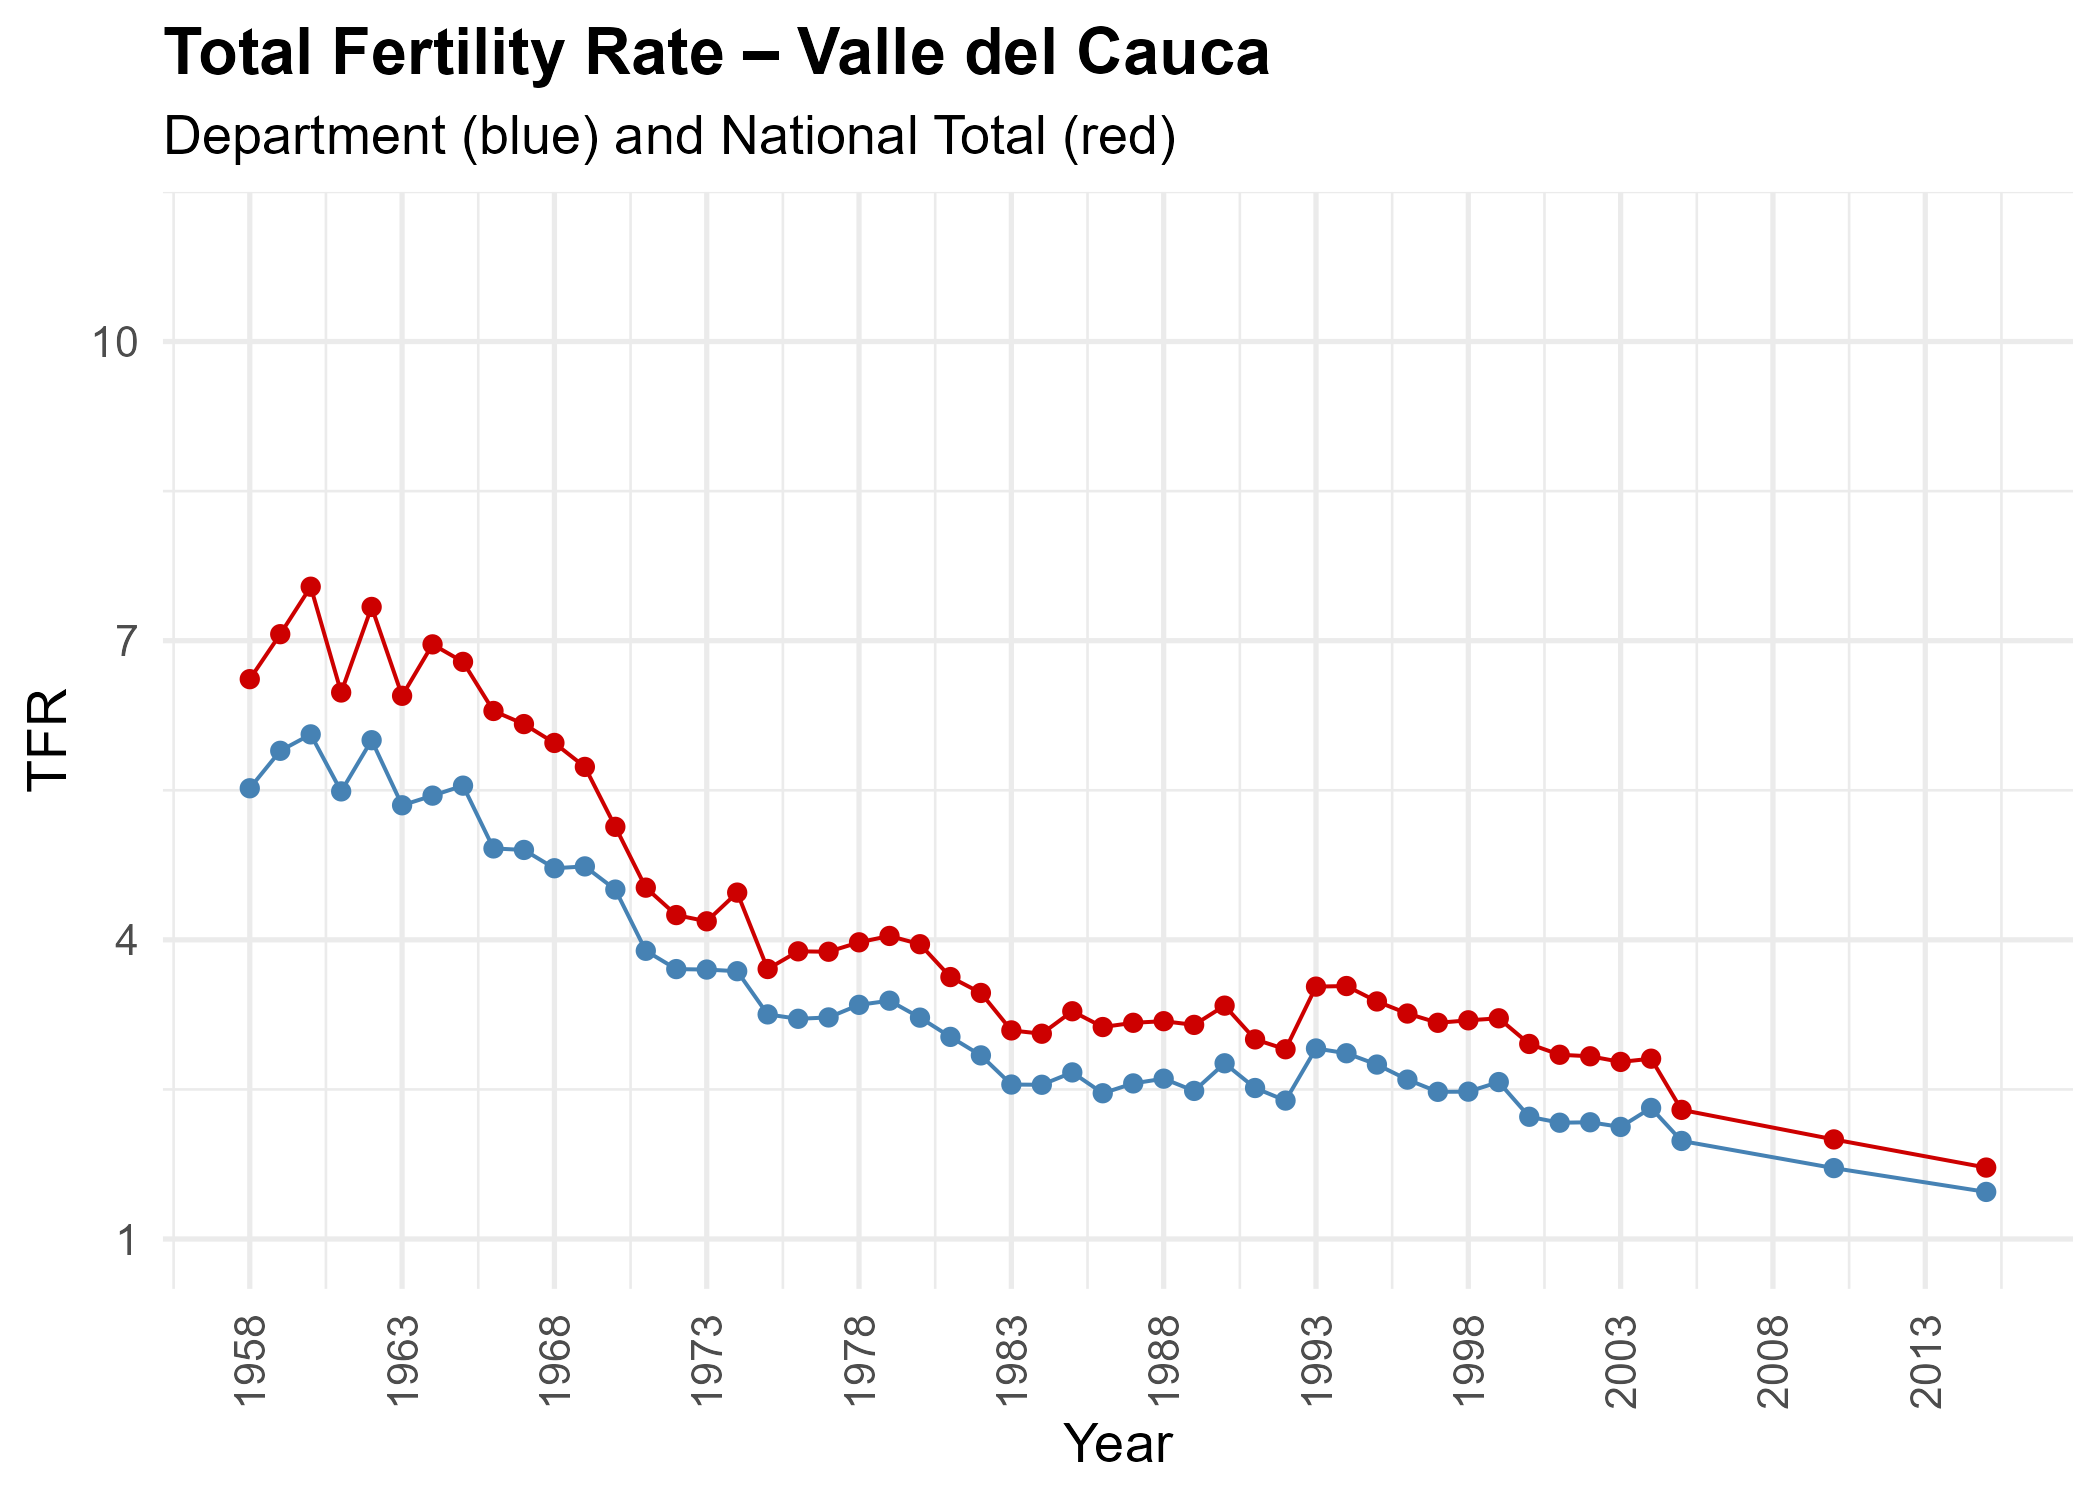
\includegraphics[height=0.78\textheight]{tfr_departamental/TFR_Valle del Cauca_vs_National.png}
\end{center}
\end{frame}
\section{Fecundidad cohortal completada}

\begin{frame}{Las cohortes cuentan la misma historia}
Las mujeres nacidas entre 1910 y 1930 completaron su vida f\'ertil con
unos \alert{6 hijos} (6{,}7 si fueron madres). La ruptura llega con las
nacidas en los a\~nos treinta y cuarenta, y se acelera despu\'es.
\bigskip
\begin{center}
\begin{tabular}{lcccc}
\toprule
Cohorte & Mujeres & FCC & FCC condicional & Fuente \\
\midrule
1910 & 2.904 & 5{,}99 & 6{,}67 & IPUMS \\
1920 & 13.007 & 6{,}17 & 6{,}75 & IPUMS \\
1930 & 20.028 & 6{,}18 & 6{,}69 & IPUMS \\
1940 & 23.545 & 5{,}40 & 5{,}94 & IPUMS \\
1950 & 15.751 & 4{,}18 & 4{,}76 & IPUMS \\
1956 & 983.765 & 3{,}05 & 3{,}51 & CNPV 2018 \\
1961 & 1.222.507 & 2{,}78 & 3{,}20 & CNPV 2018 \\
1966 & 1.381.253 & 2{,}57 & 2{,}96 & CNPV 2018 \\
\bottomrule
\end{tabular}
\end{center}
\medskip
La fecundidad cohortal confirma que la ca\'ida no es aplazamiento
(calendario), sino \alert{reducci\'on real del tama\~no de las familias}.
\end{frame}
\begin{frame}{FCC departamental, cohortes seleccionadas}
\begin{center}
{\tiny\begin{tabular}{lcccc}\toprule
Departamento & Cohorte 1915 & 1930 & 1945 & 1961$^{*}$ \\ \midrule
Amazonas & , & 6{,}60 & 5{,}15 & 4{,}09 \\
Antioquia & 6{,}59 & 6{,}58 & 4{,}88 & 2{,}49 \\
Arauca & 10{,}00 & 7{,}05 & 6{,}18 & 3{,}96 \\
Atlántico & 5{,}39 & 5{,}97 & 4{,}24 & 2{,}60 \\
Bogotá D.C. & 5{,}30 & 5{,}35 & 3{,}84 & 2{,}41 \\
Bolívar & 6{,}32 & 6{,}76 & 5{,}28 & 3{,}27 \\
Boyacá & 5{,}86 & 6{,}24 & 5{,}40 & 3{,}28 \\
Caldas & 6{,}41 & 6{,}63 & 3{,}97 & 2{,}45 \\
Caquetá & 9{,}21 & 7{,}56 & 6{,}29 & 4{,}03 \\
Cauca & 6{,}86 & 6{,}19 & 4{,}54 & 3{,}35 \\
Cesar & 7{,}06 & 6{,}95 & 5{,}28 & 3{,}45 \\
Chocó & 7{,}94 & 7{,}64 & 6{,}18 & 3{,}88 \\
Córdoba & 6{,}59 & 6{,}70 & 5{,}60 & 3{,}35 \\
Huila & 7{,}18 & 6{,}64 & 5{,}66 & 3{,}52 \\
La Guajira & 5{,}17 & 7{,}70 & 4{,}88 & 3{,}45 \\
Meta & 6{,}43 & 6{,}79 & 5{,}23 & 3{,}25 \\
Nariño & 5{,}69 & 5{,}66 & 4{,}79 & 3{,}20 \\
Putumayo & 9{,}40 & 7{,}17 & 6{,}28 & 4{,}02 \\
San Andrés & 3{,}50 & 4{,}00 & 3{,}81 & 2{,}43 \\
Santander & 5{,}86 & 6{,}30 & 5{,}07 & 2{,}82 \\
Tolima & 6{,}58 & 6{,}48 & 4{,}88 & 2{,}92 \\
Valle del Cauca & 5{,}68 & 5{,}71 & 4{,}21 & 2{,}42 \\
\bottomrule\end{tabular}}
\end{center}
{\scriptsize $^{*}$Cohorte 1961: CNPV 2018. San Andr\'es, otra vez, es
el caso at\'ipico: FCC de 3{,}5,4 cuando el resto del pa\'is estaba en
6,10. Fuente: c\'alculos propios.}
\end{frame}

\begin{frame}{A continuaci\'on: FCC por departamento}
Para cada departamento, dos series frente al total nacional: la FCC de
\alert{todas} las mujeres y la FCC \alert{condicional} a haber sido
madre. La brecha entre ambas es la huella de la infecundidad.
\end{frame}
\begin{frame}{FCC: Amazonas}
\begin{columns}
\column{0.5\textwidth}\centering
{\small Todas las mujeres}\\
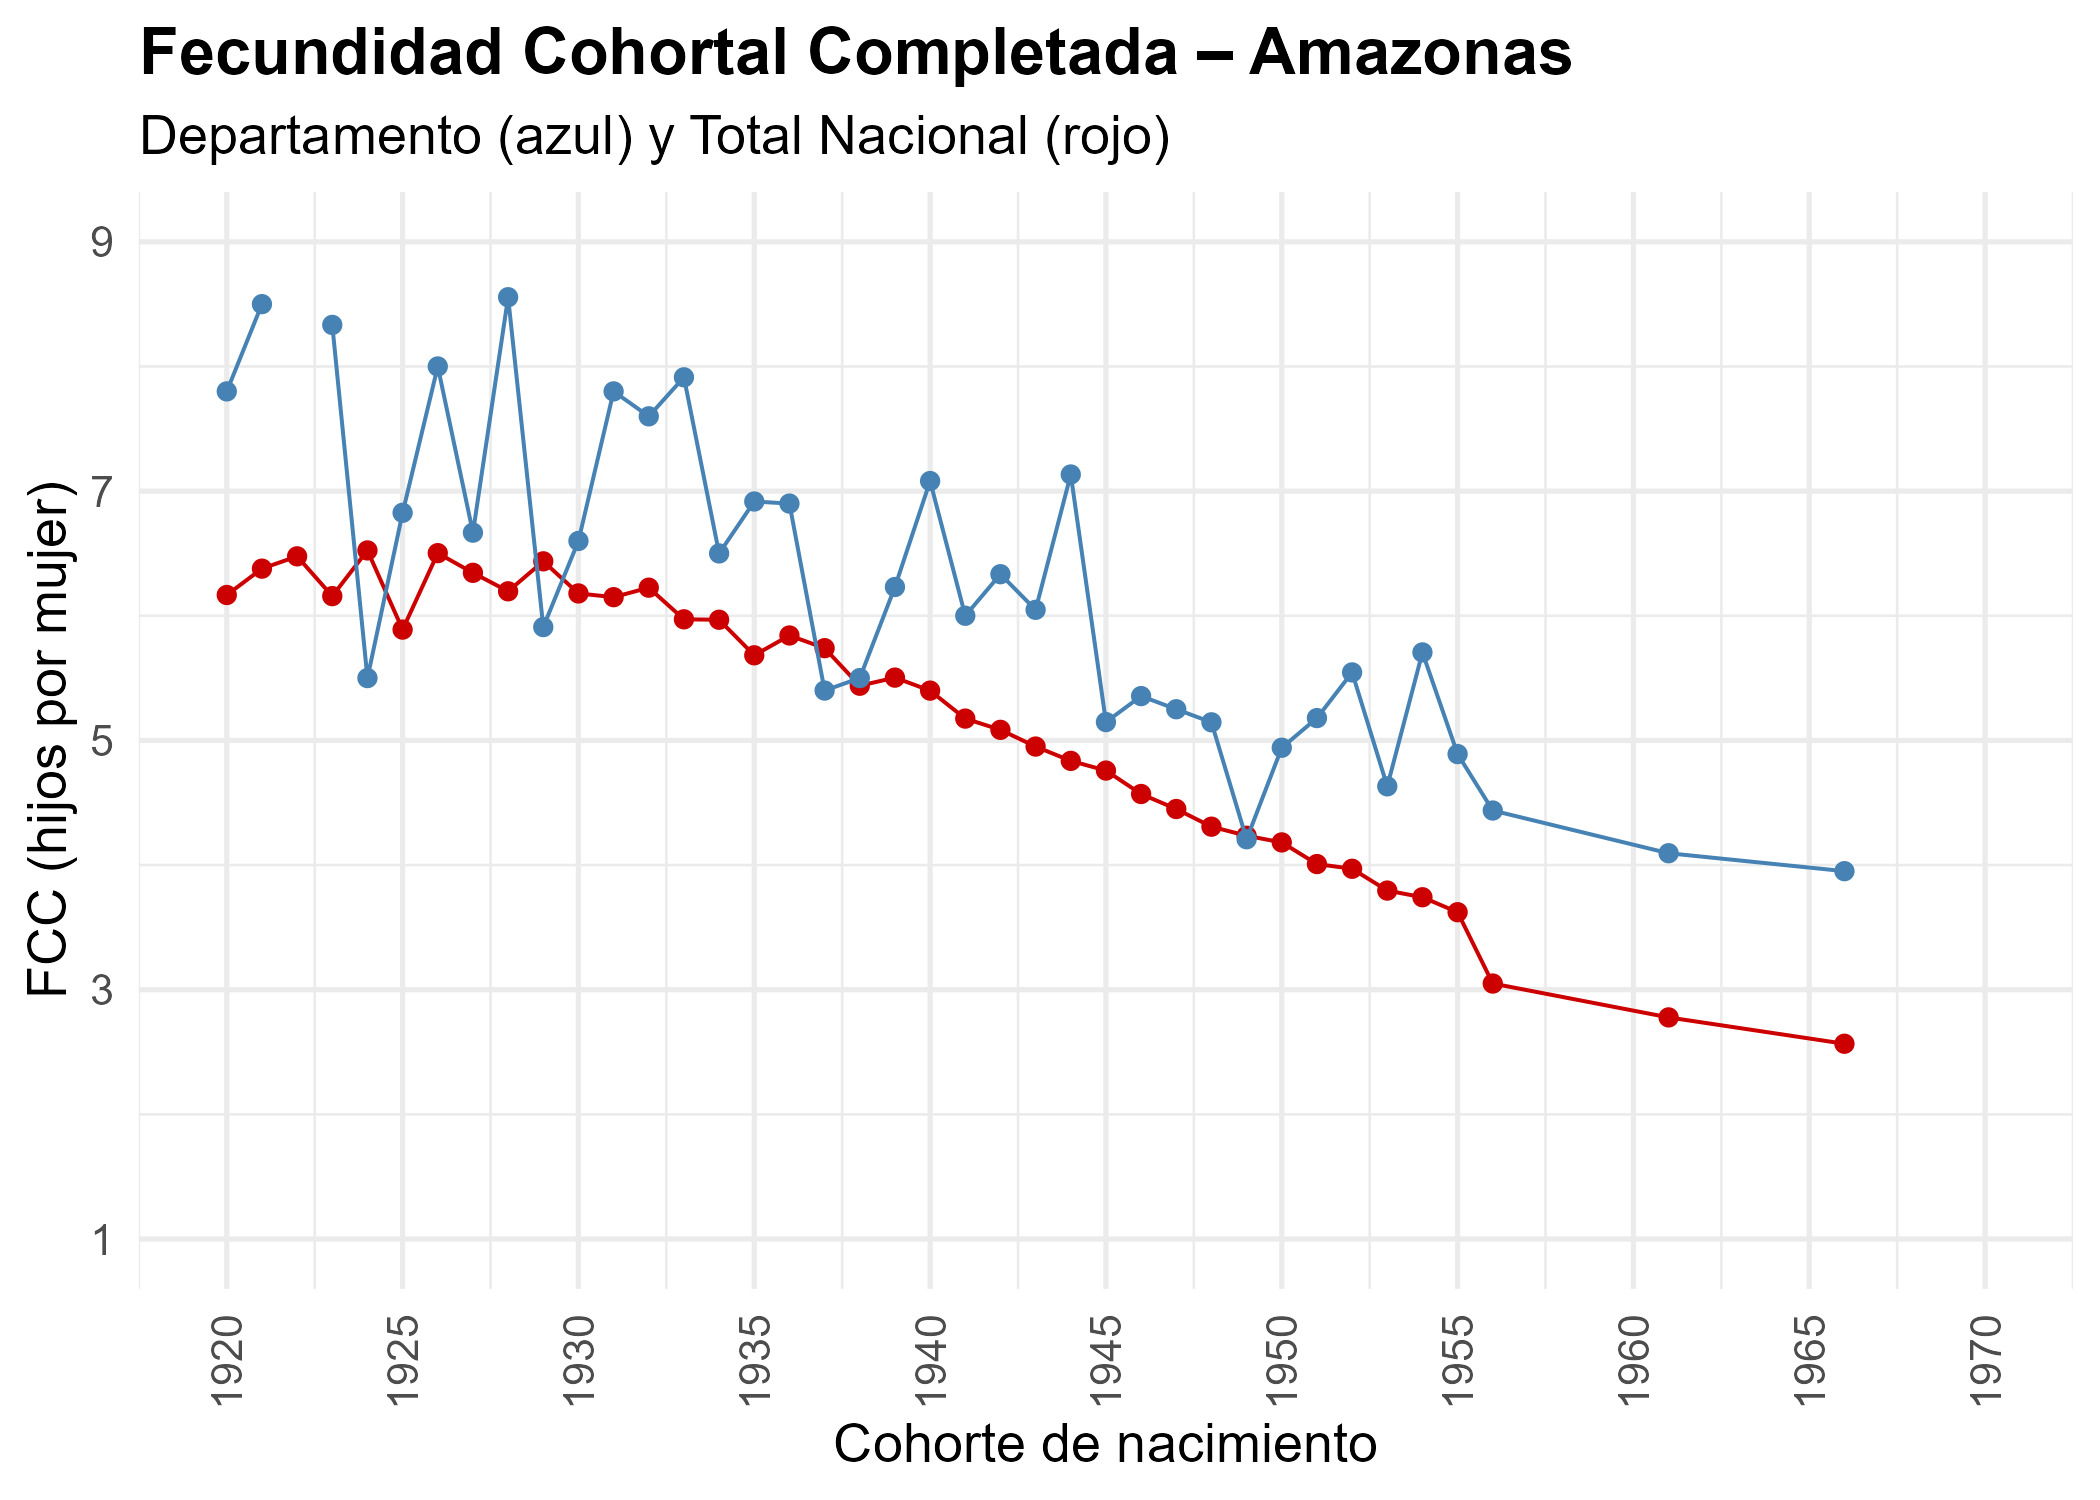
\includegraphics[width=\textwidth]{fcc_departamental/FCC_Amazonas_vs_National.png}
\column{0.5\textwidth}\centering
{\small Condicional (madres)}\\
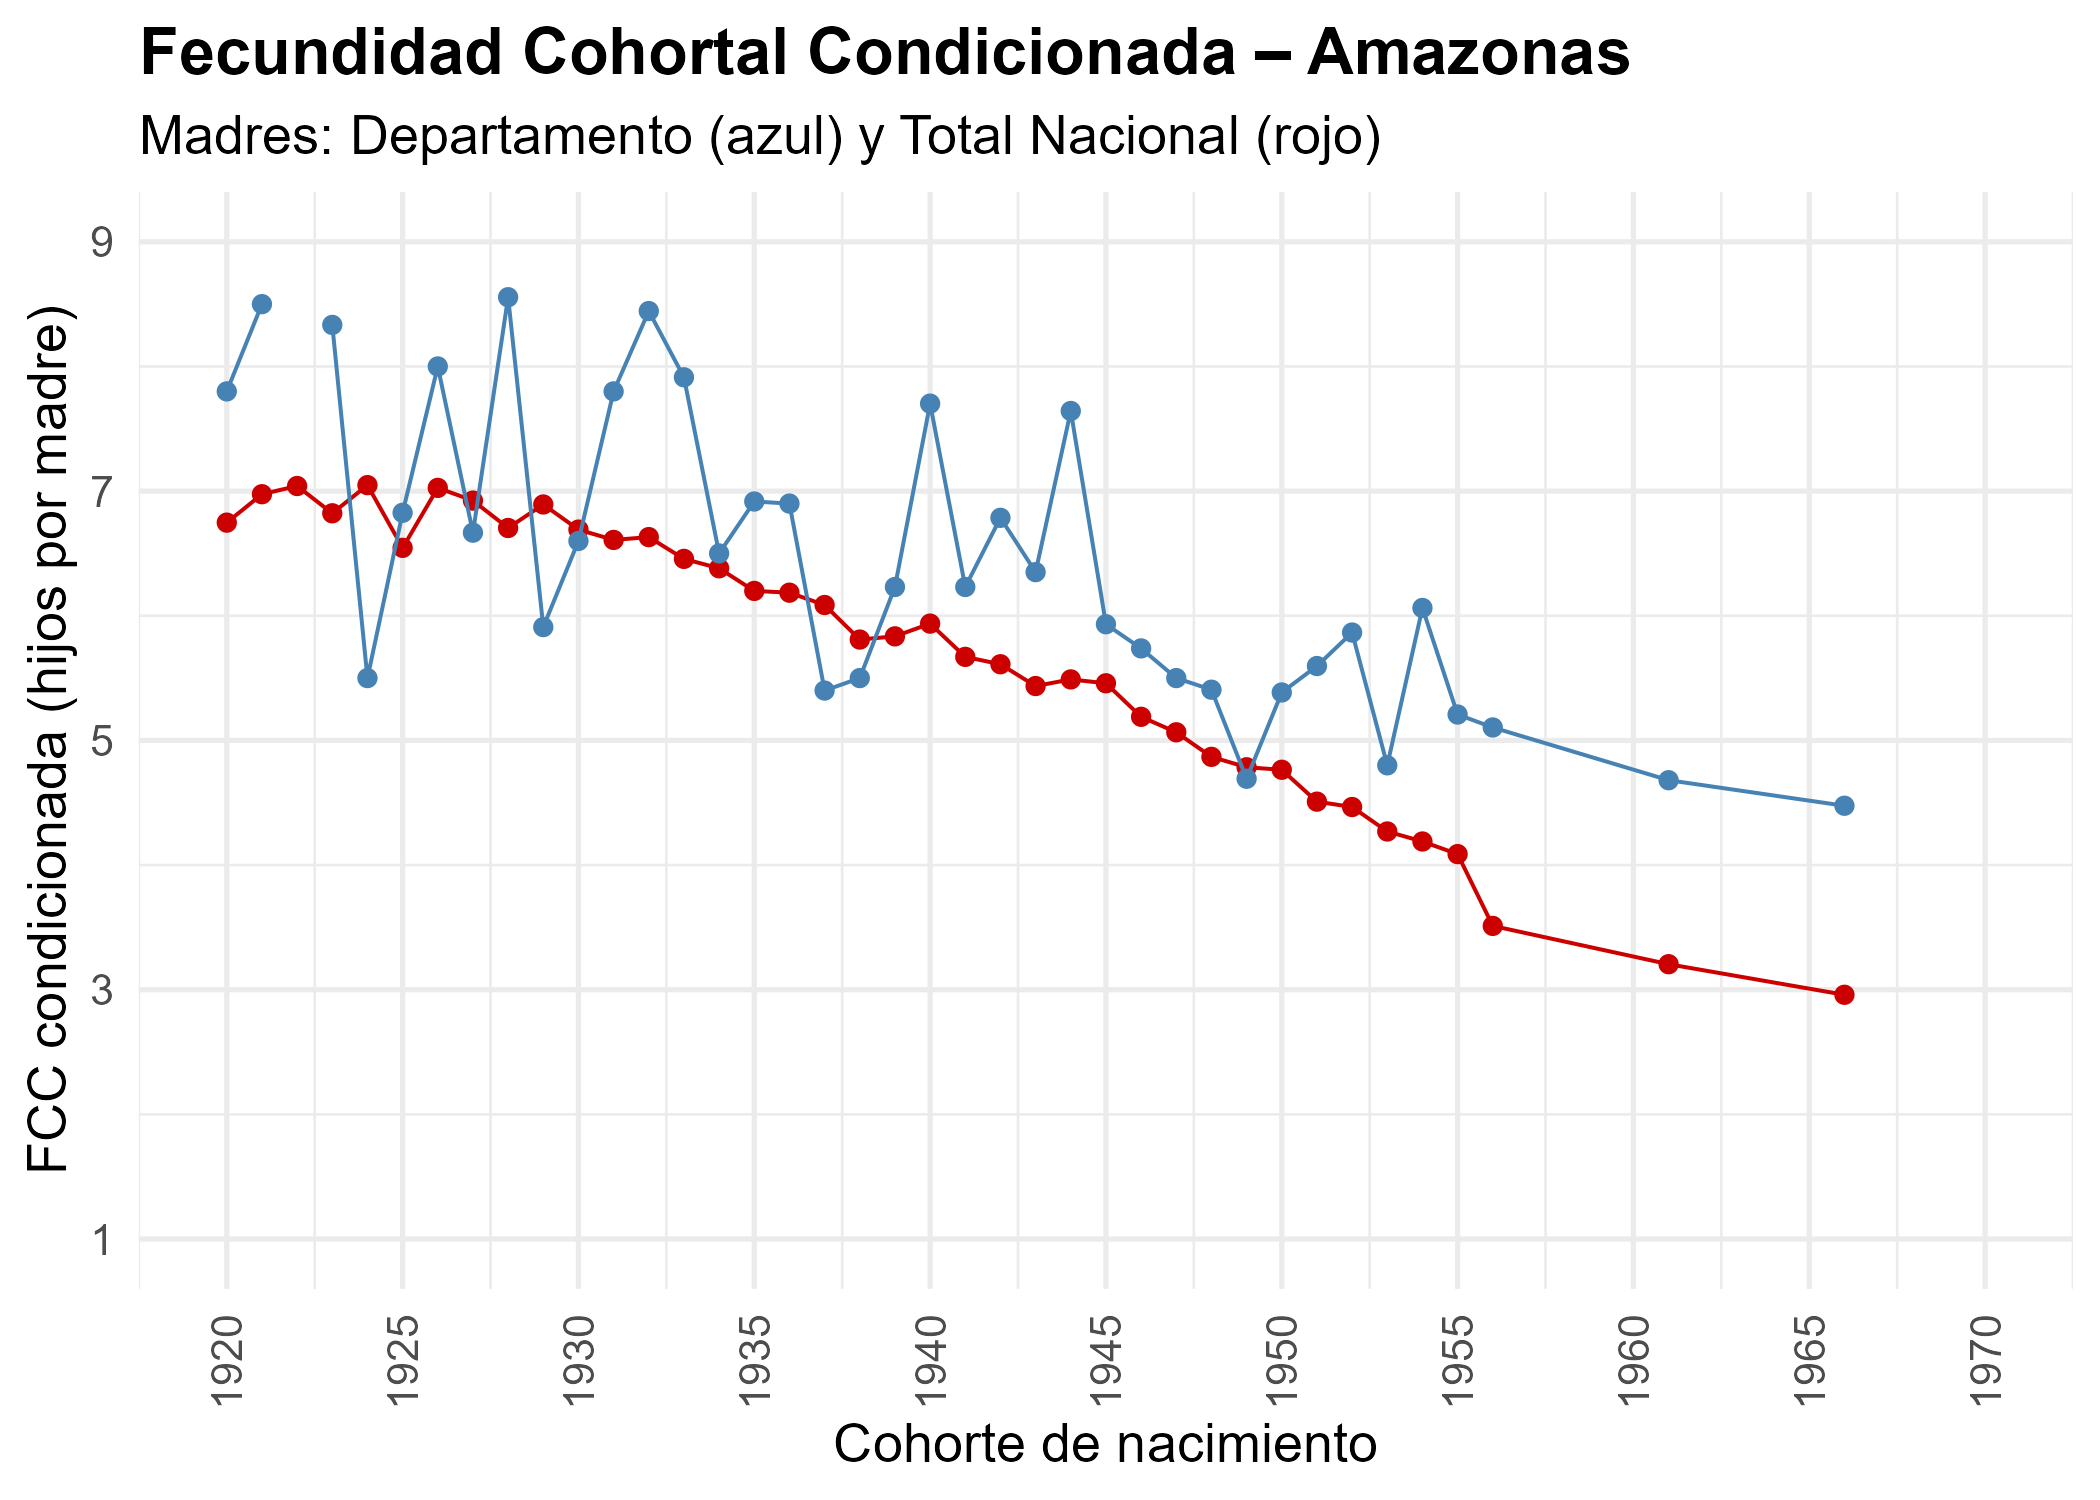
\includegraphics[width=\textwidth]{fcc_departamental/FCC_cond_Amazonas_vs_National.png}
\end{columns}
\end{frame}
\begin{frame}{FCC: Antioquia}
\begin{columns}
\column{0.5\textwidth}\centering
{\small Todas las mujeres}\\
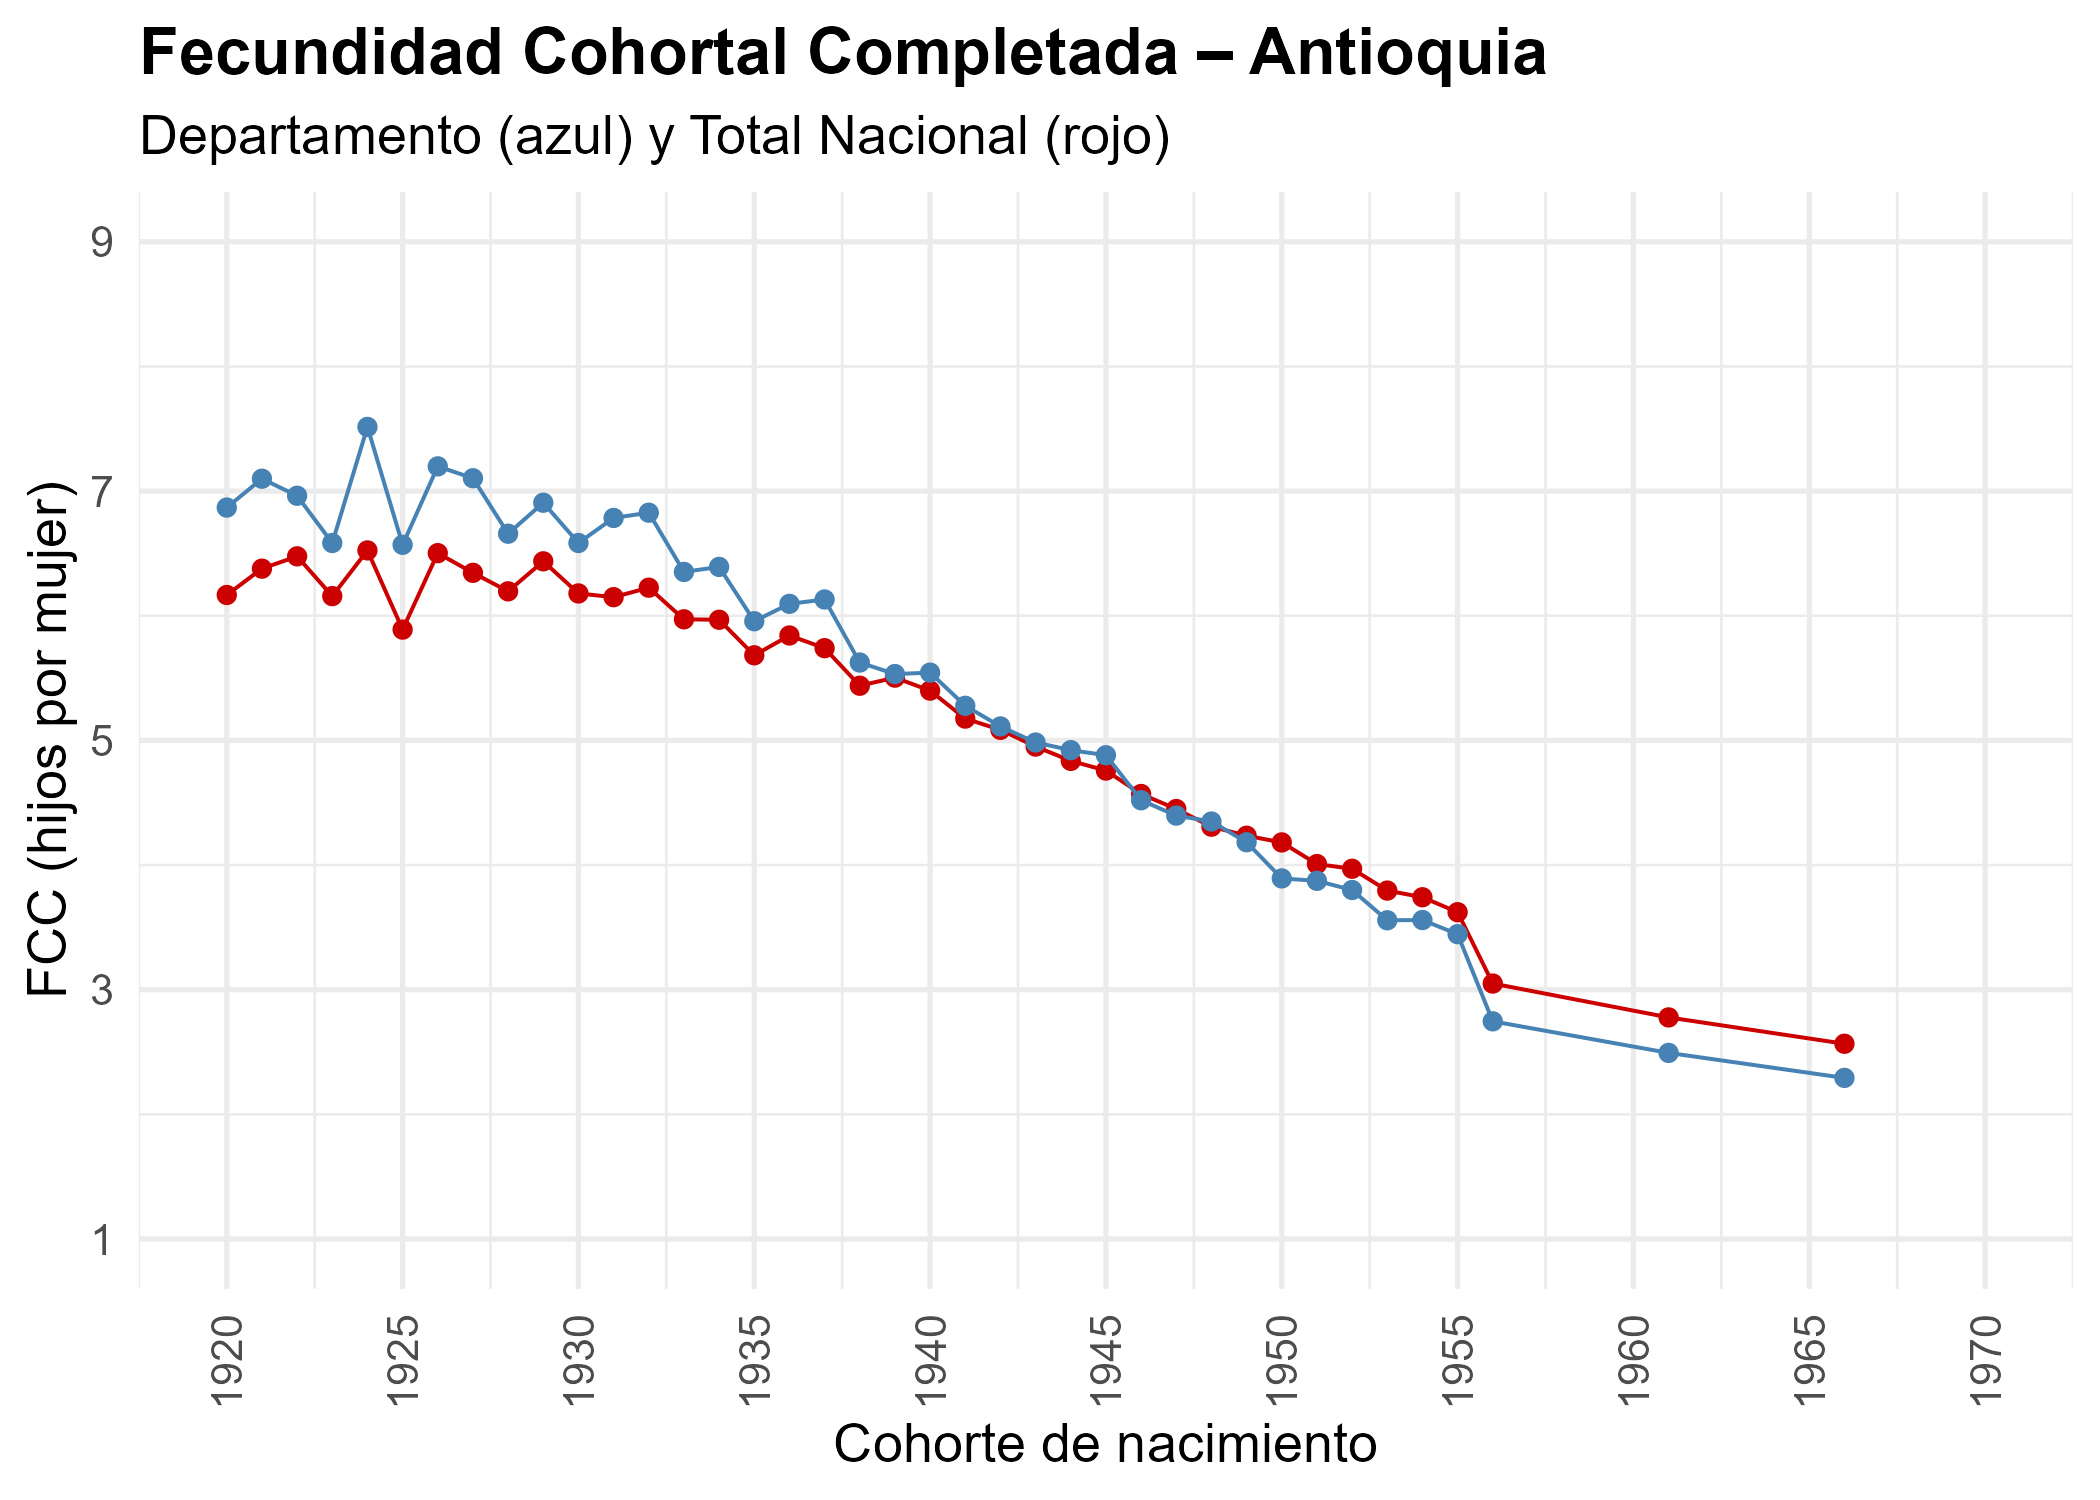
\includegraphics[width=\textwidth]{fcc_departamental/FCC_Antioquia_vs_National.png}
\column{0.5\textwidth}\centering
{\small Condicional (madres)}\\
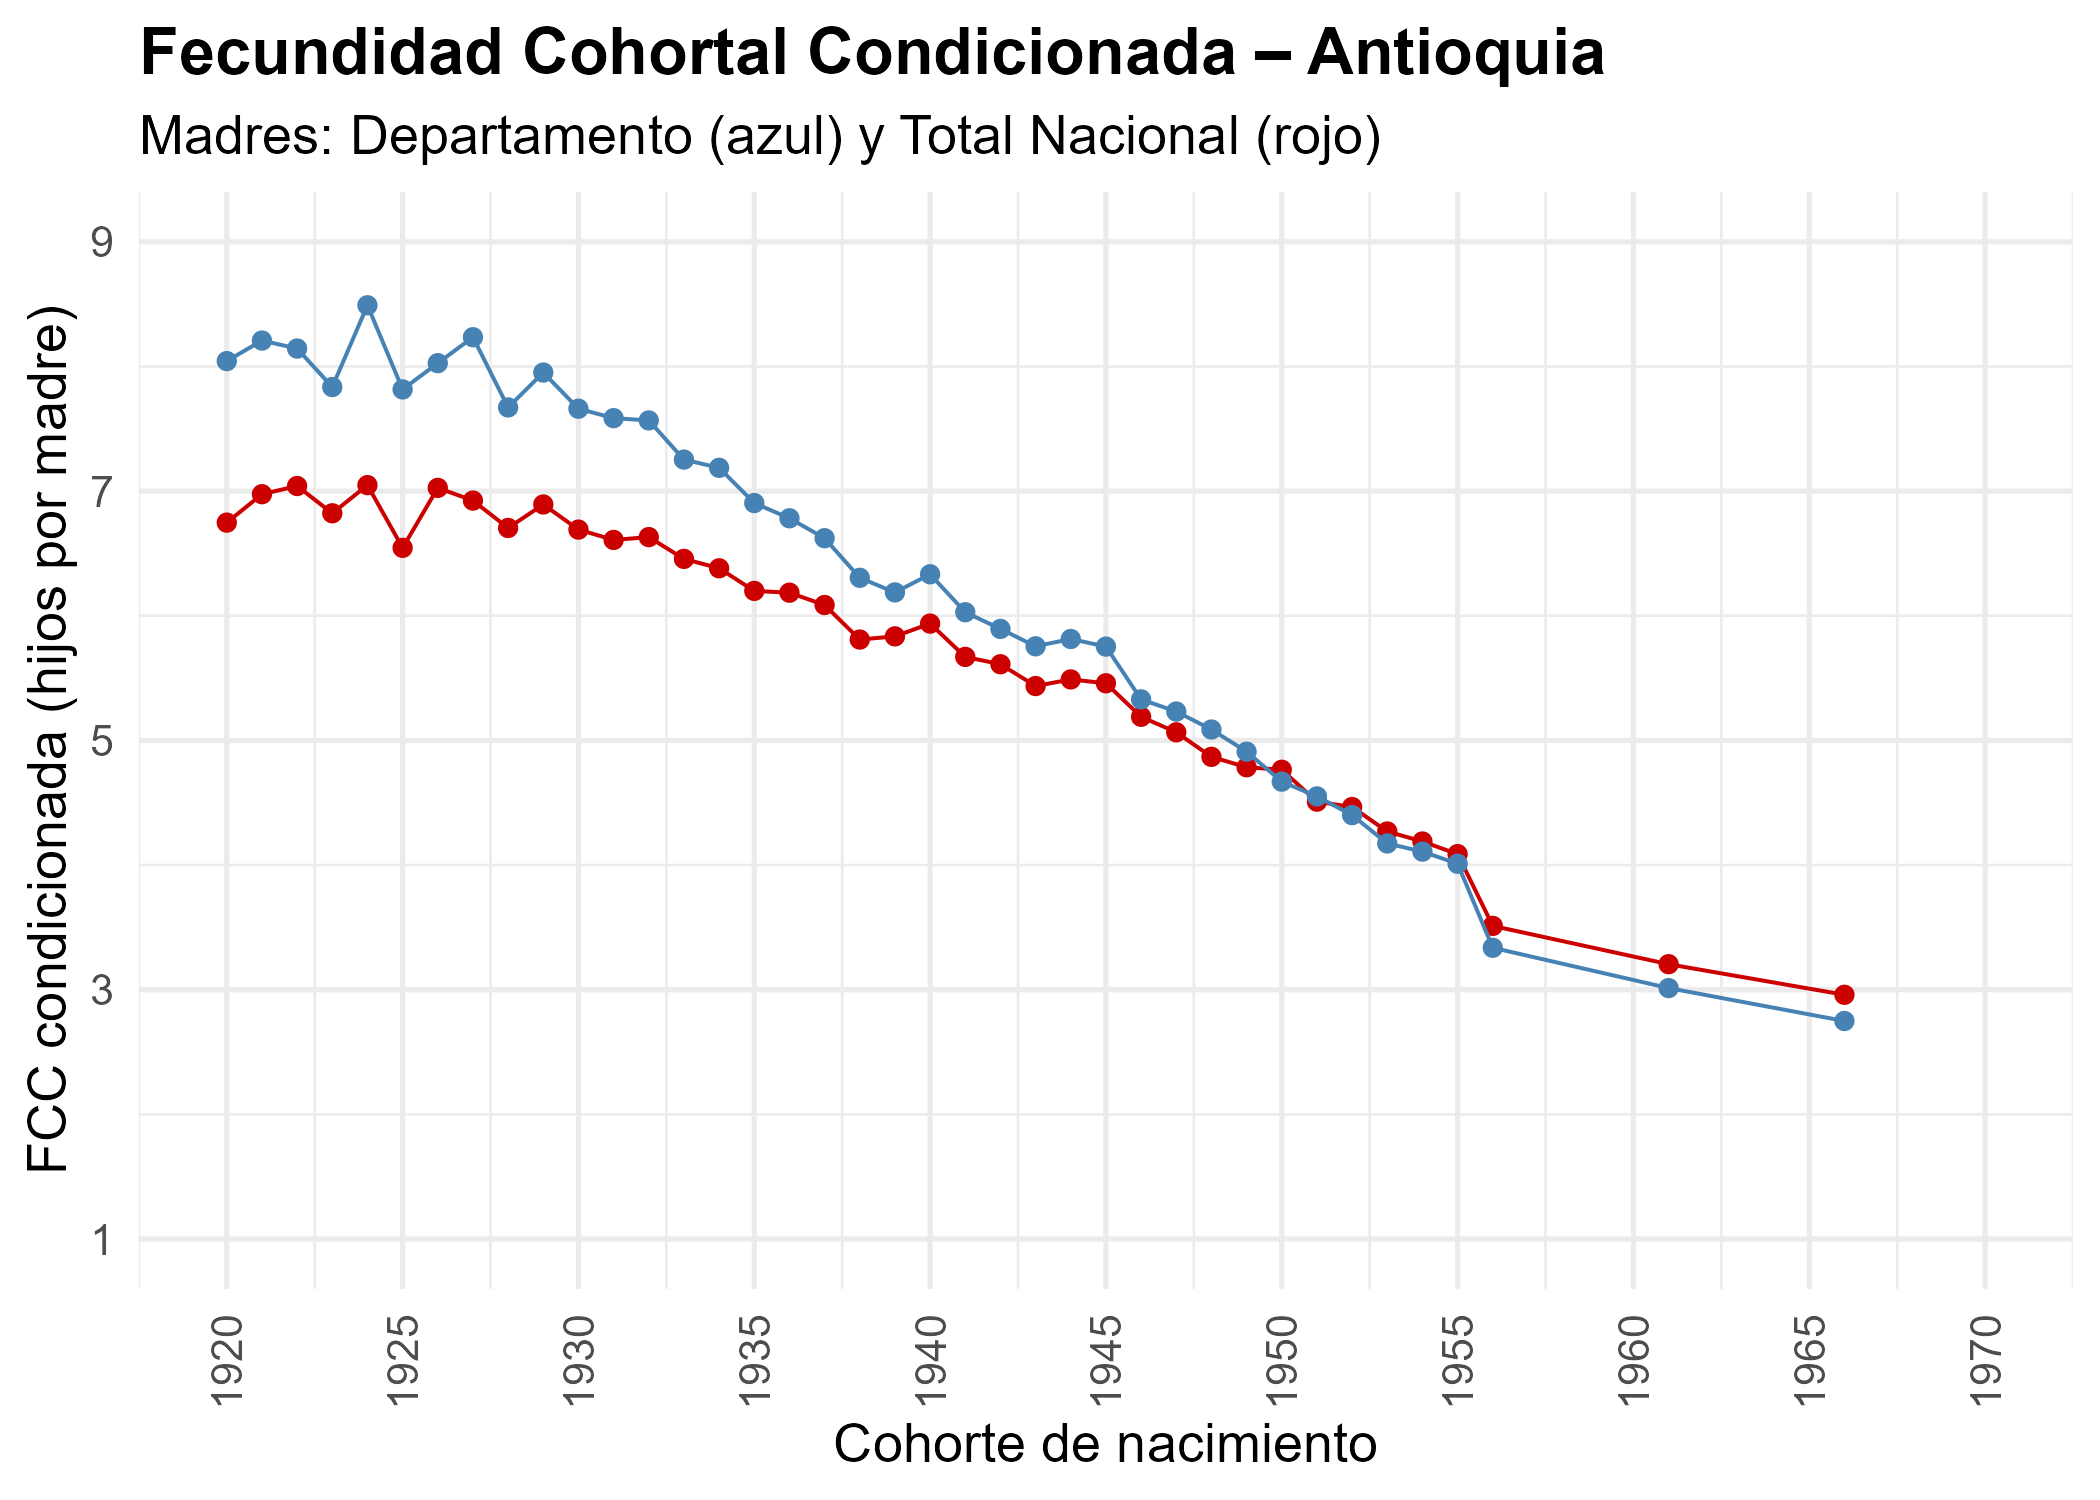
\includegraphics[width=\textwidth]{fcc_departamental/FCC_cond_Antioquia_vs_National.png}
\end{columns}
\end{frame}
\begin{frame}{FCC: Arauca}
\begin{columns}
\column{0.5\textwidth}\centering
{\small Todas las mujeres}\\
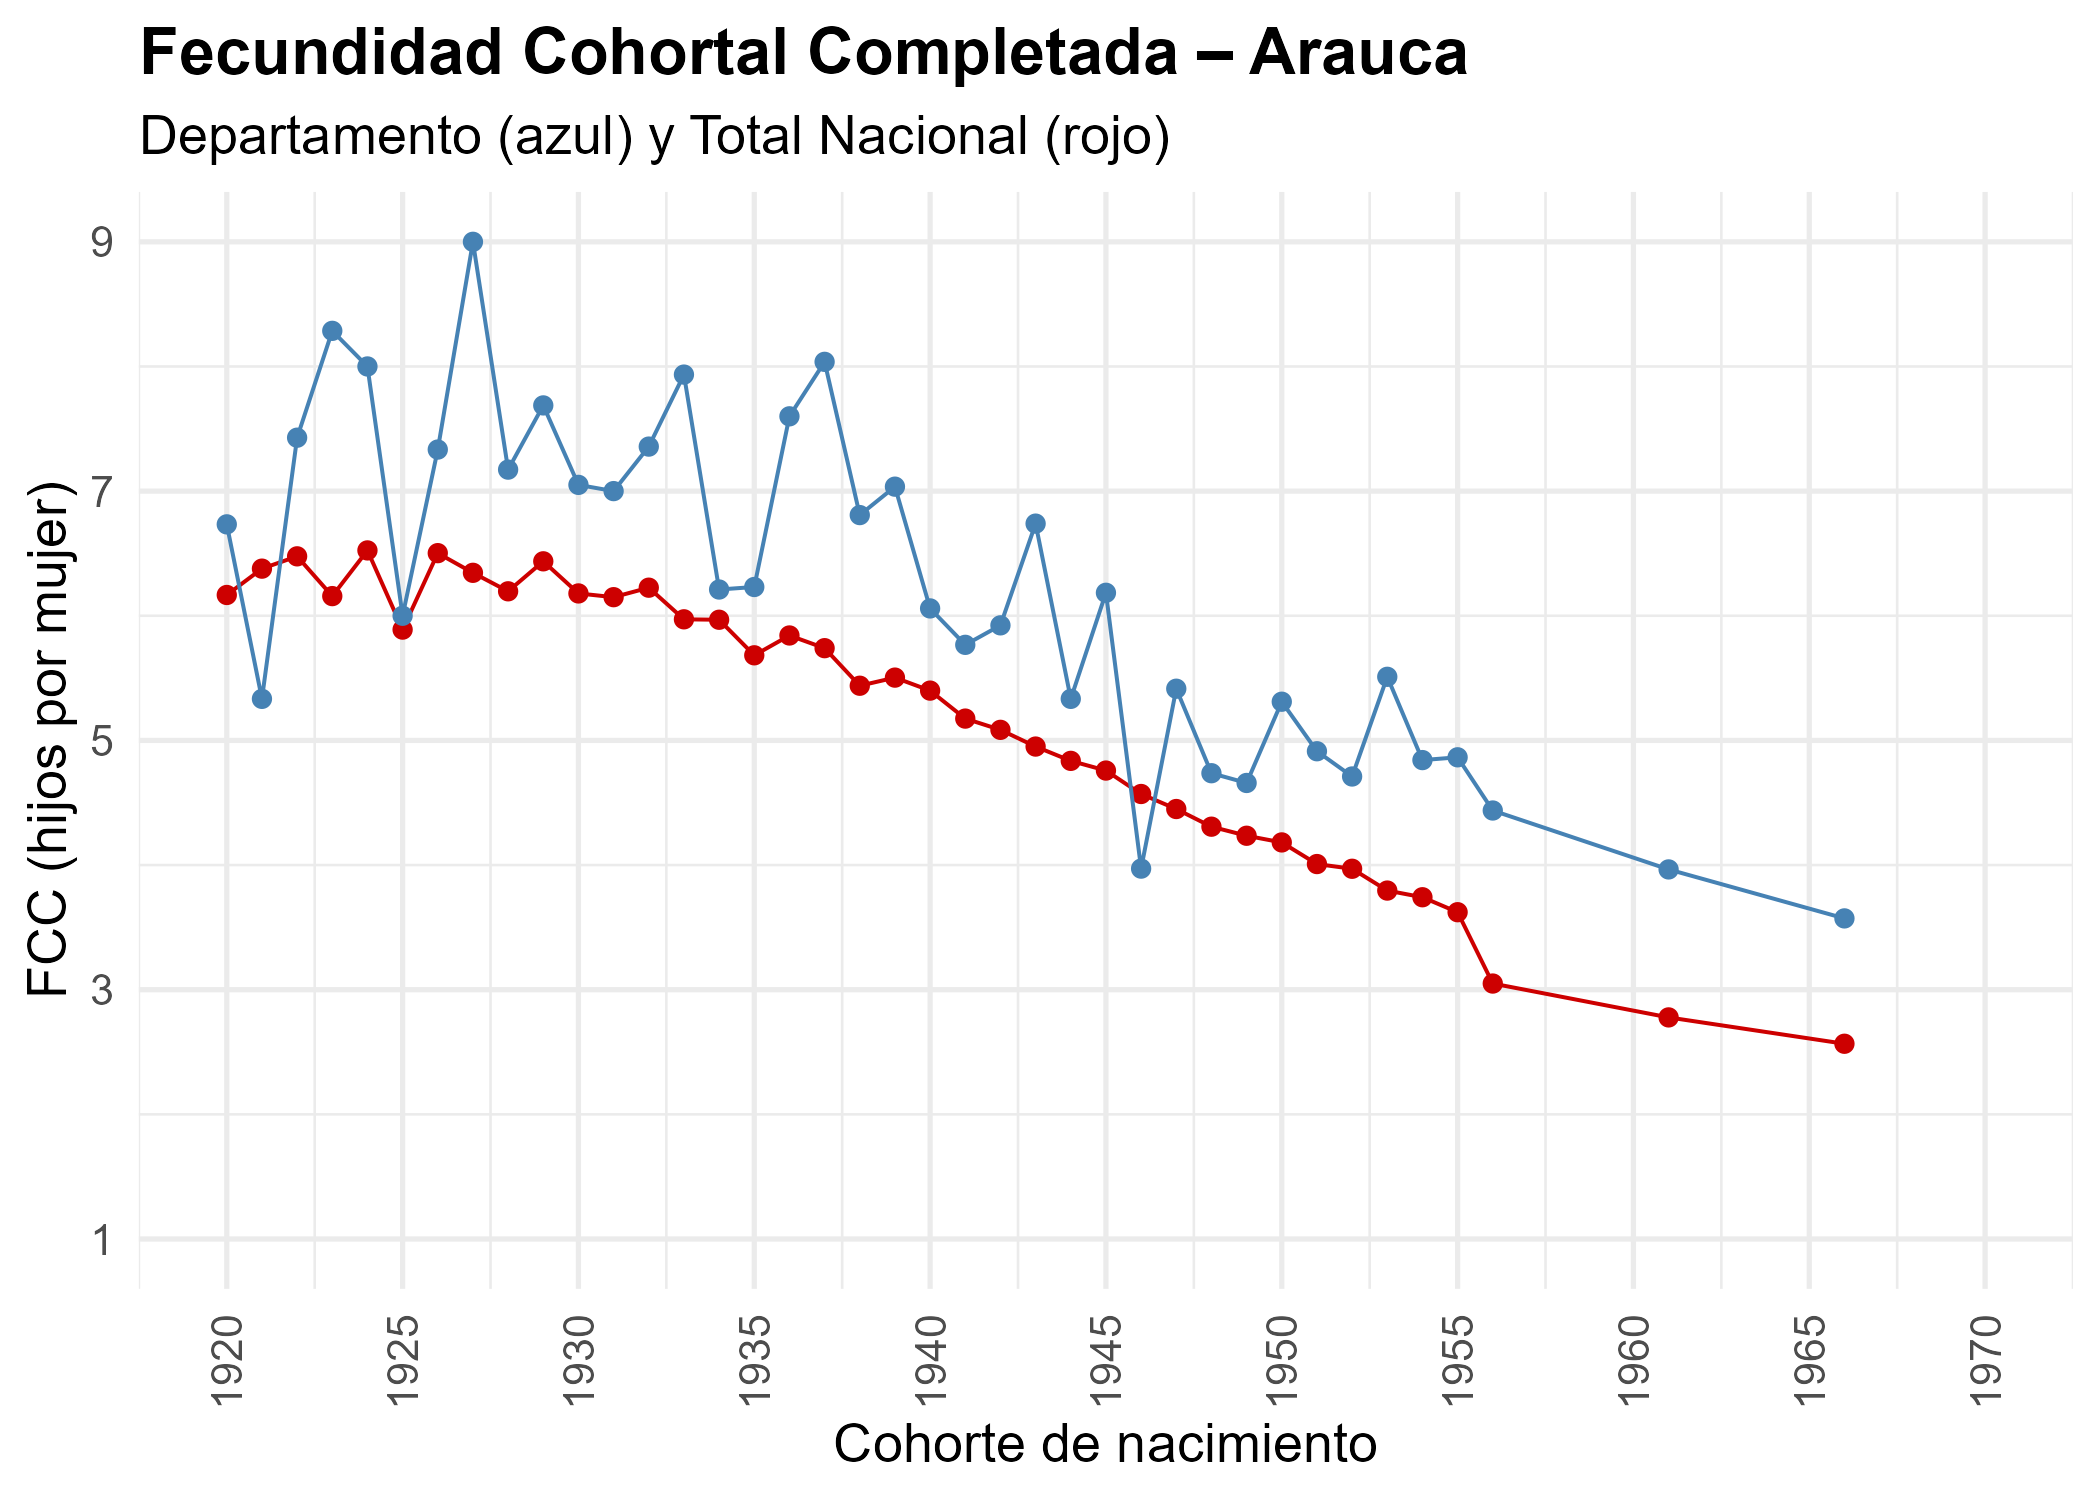
\includegraphics[width=\textwidth]{fcc_departamental/FCC_Arauca_vs_National.png}
\column{0.5\textwidth}\centering
{\small Condicional (madres)}\\
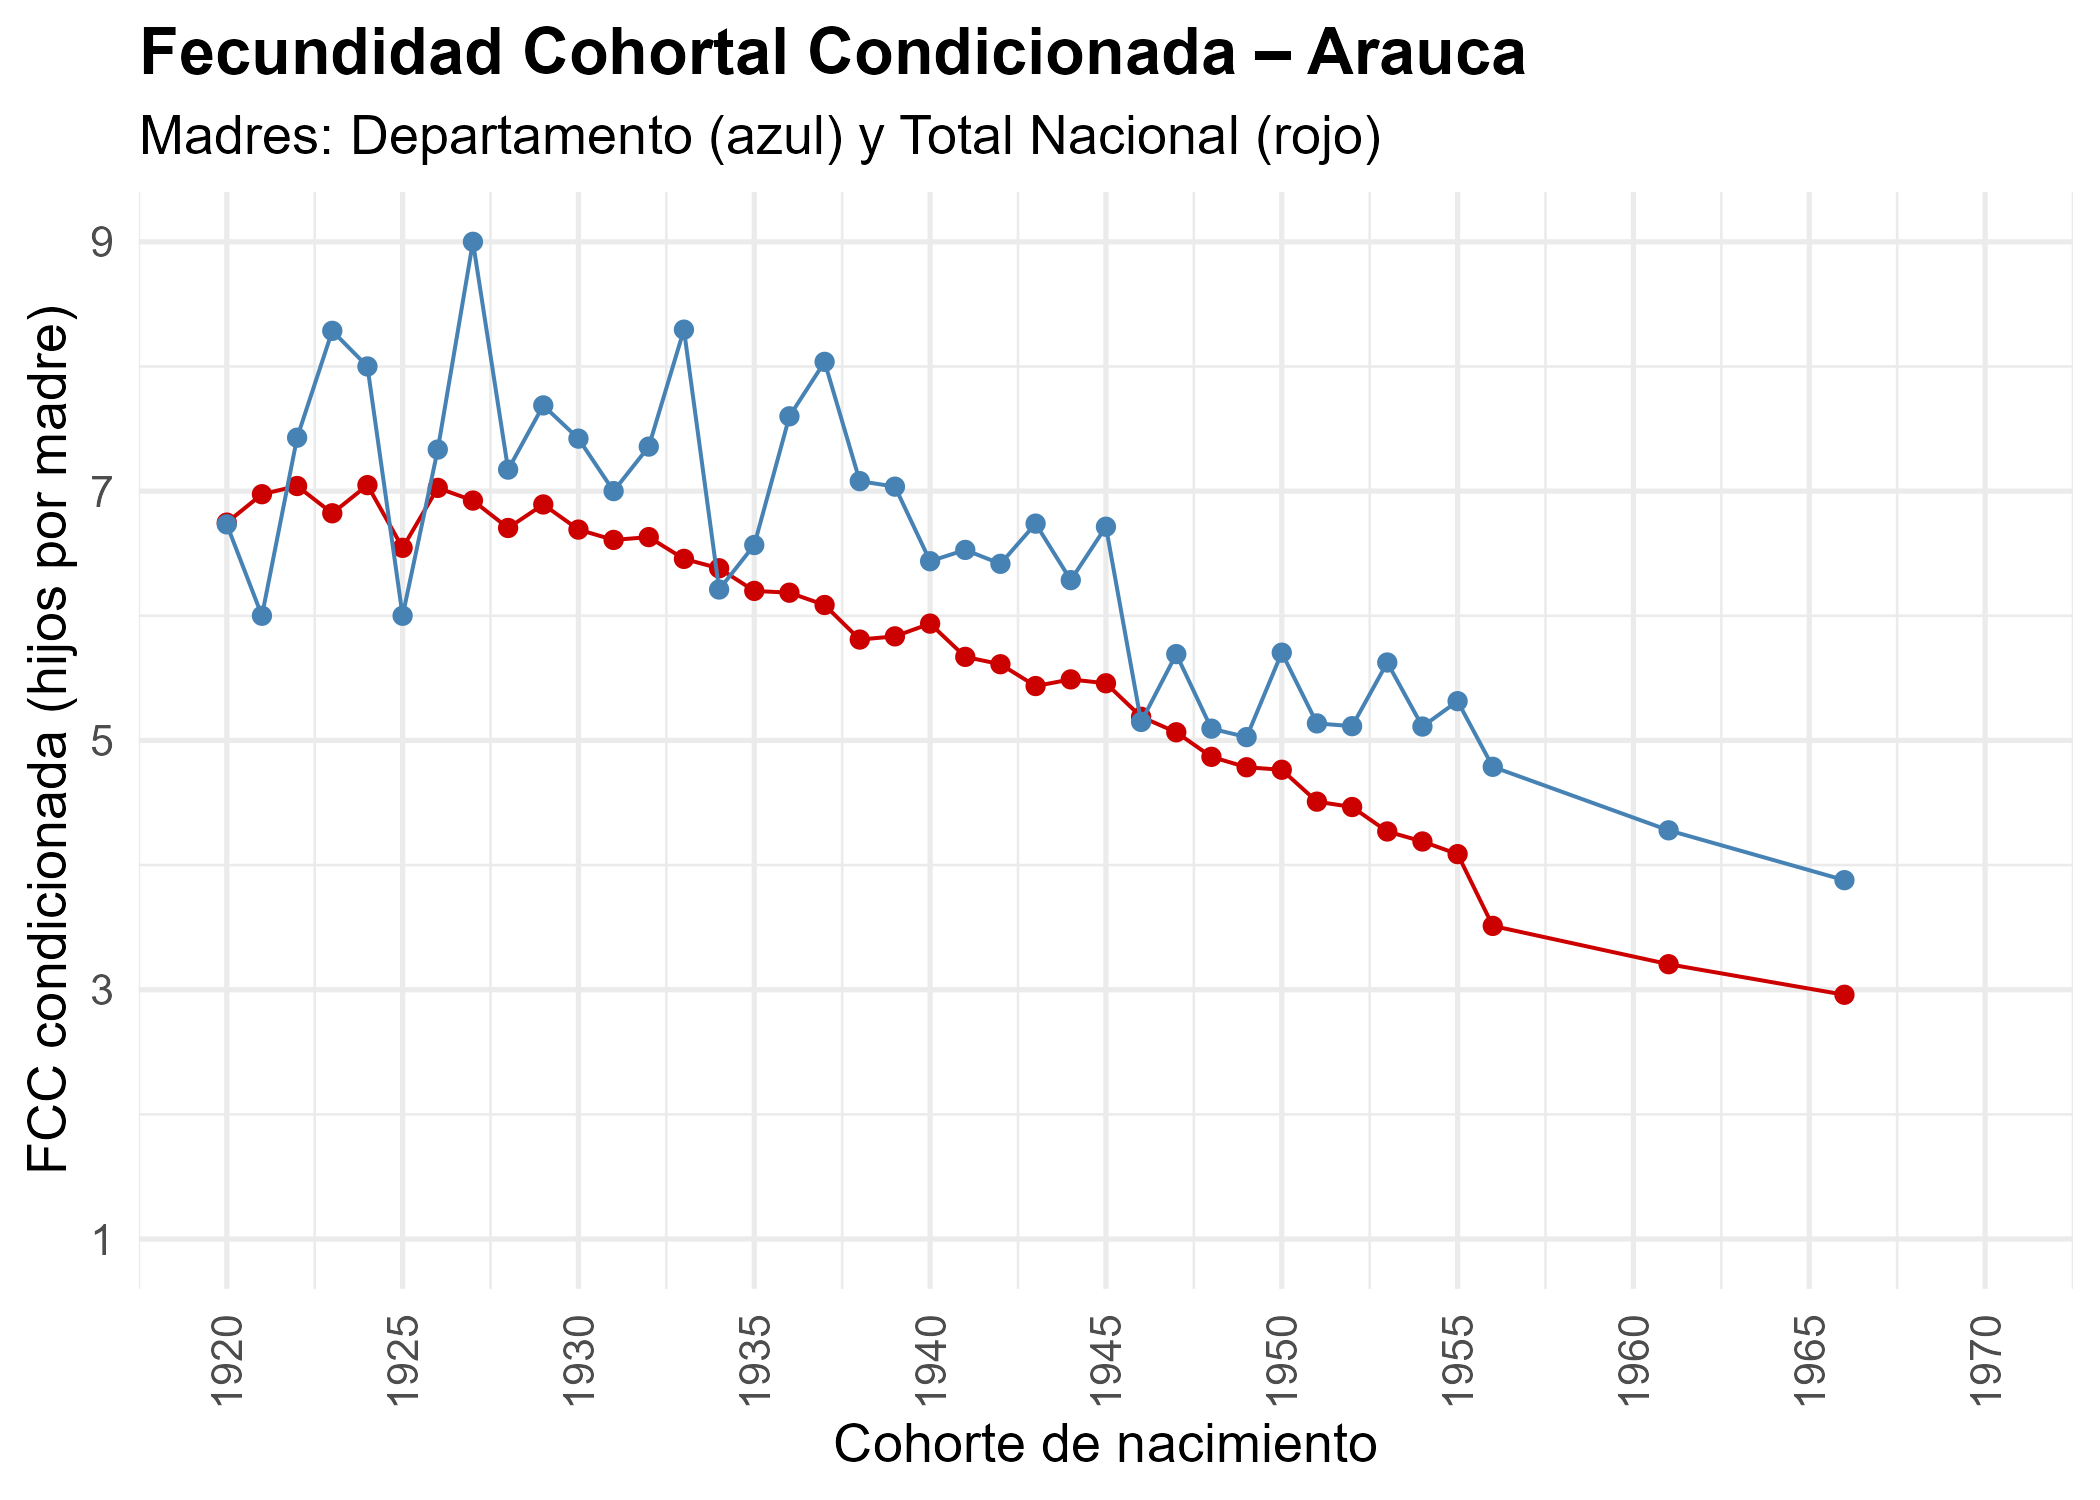
\includegraphics[width=\textwidth]{fcc_departamental/FCC_cond_Arauca_vs_National.png}
\end{columns}
\end{frame}
\begin{frame}{FCC: Atlántico}
\begin{columns}
\column{0.5\textwidth}\centering
{\small Todas las mujeres}\\
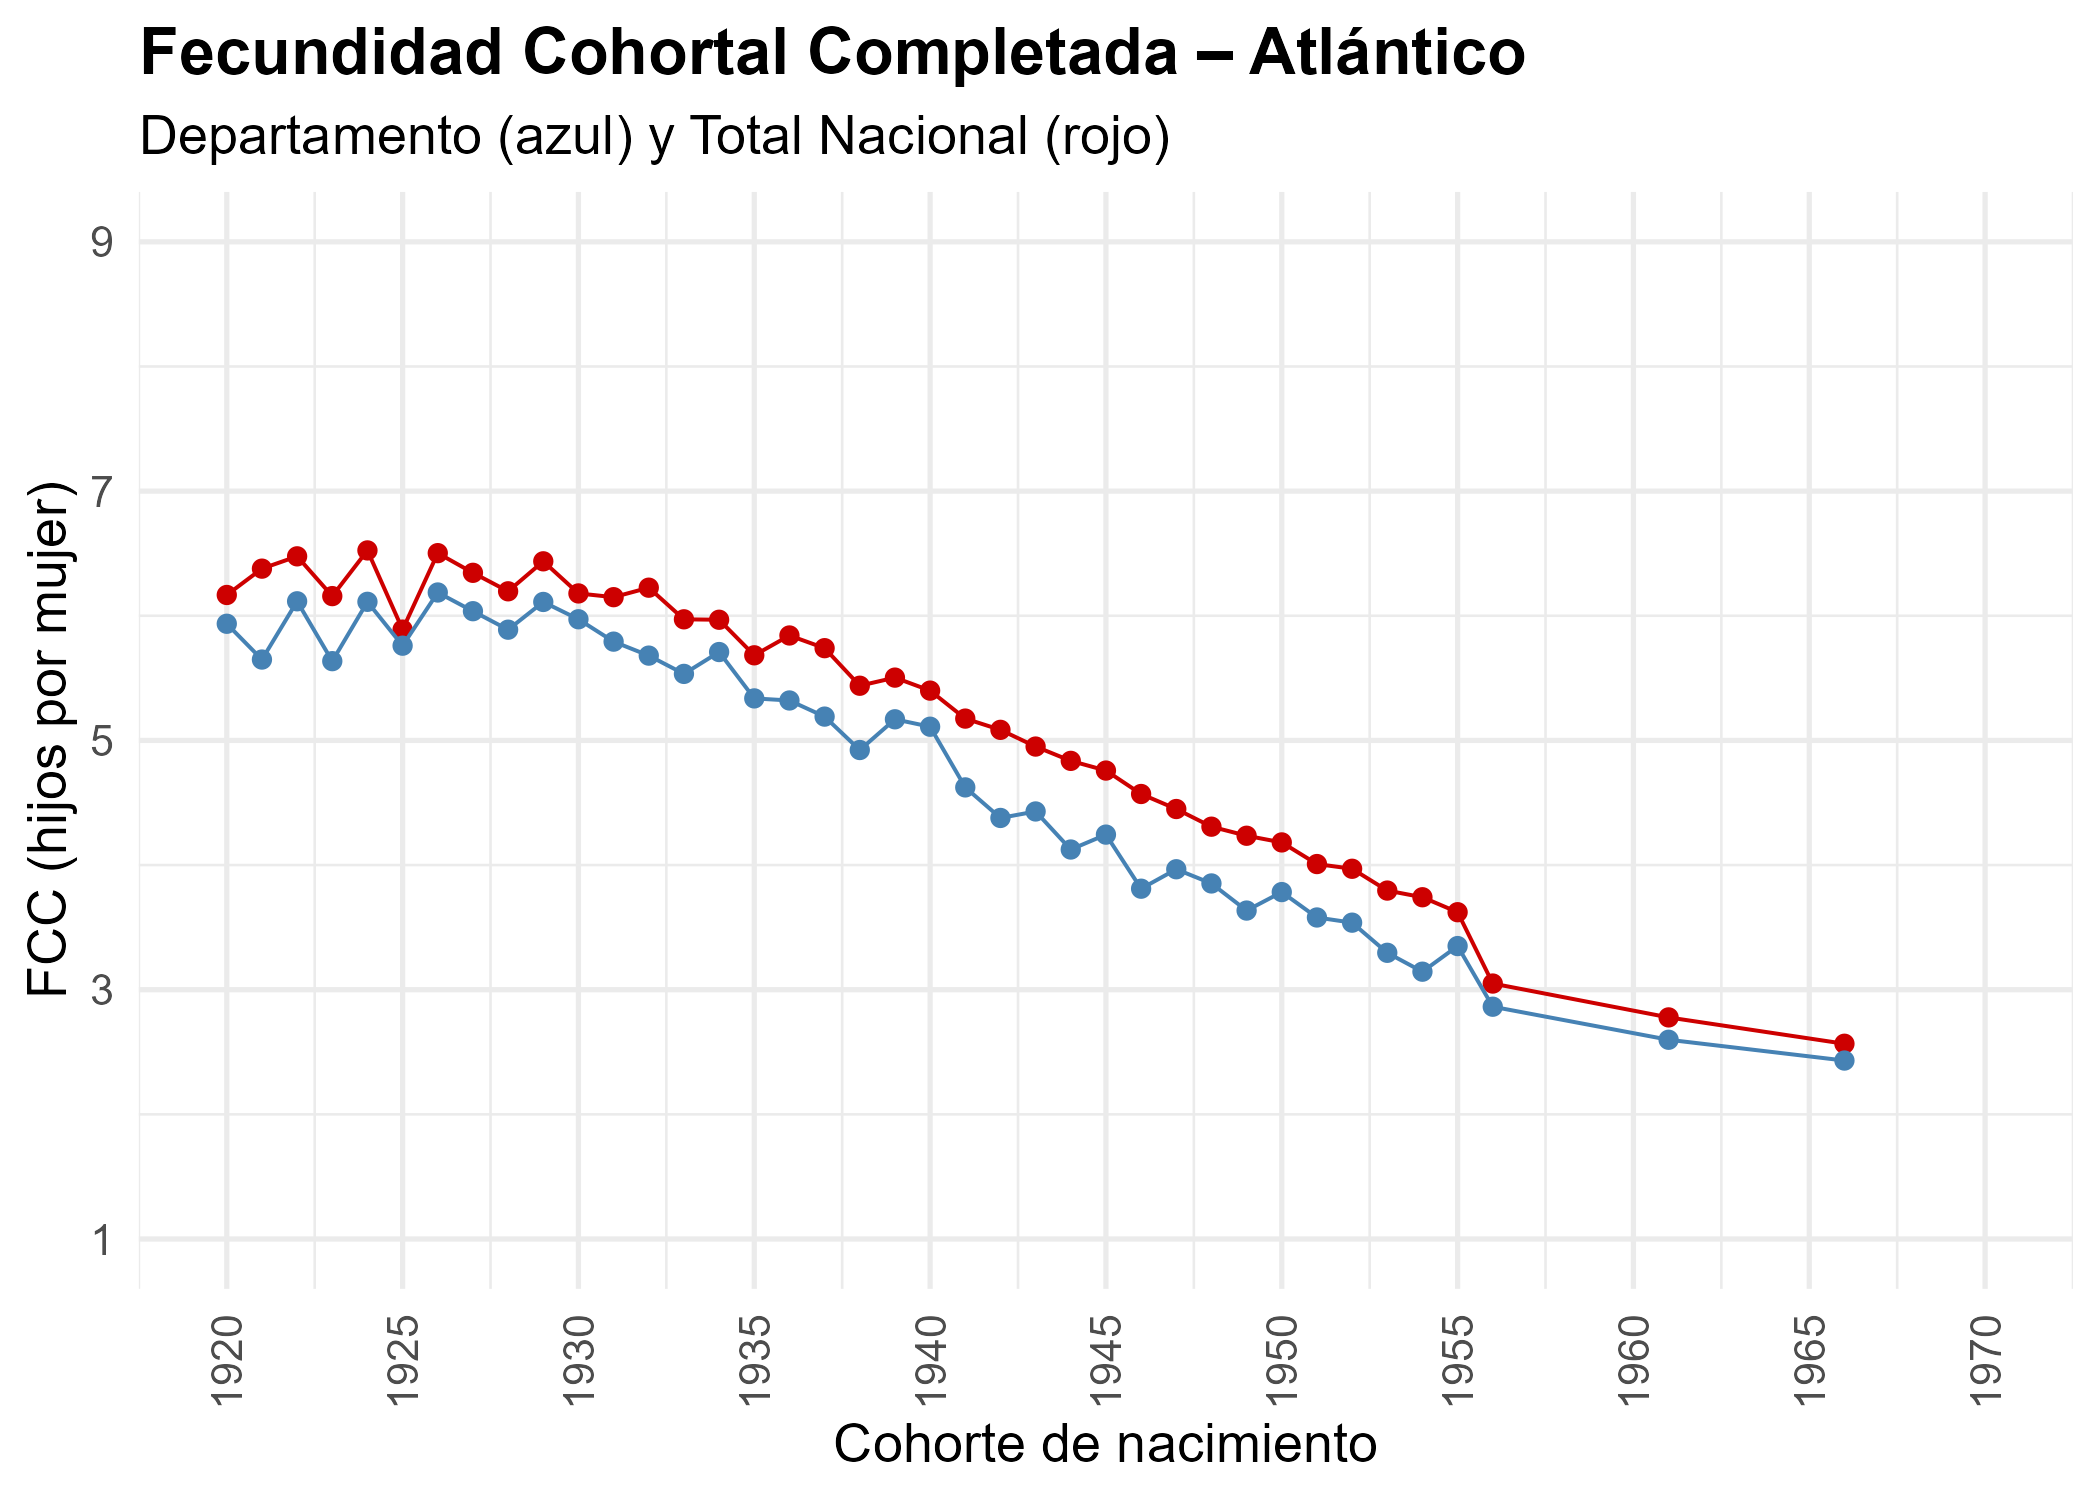
\includegraphics[width=\textwidth]{fcc_departamental/FCC_Atlántico_vs_National.png}
\column{0.5\textwidth}\centering
{\small Condicional (madres)}\\
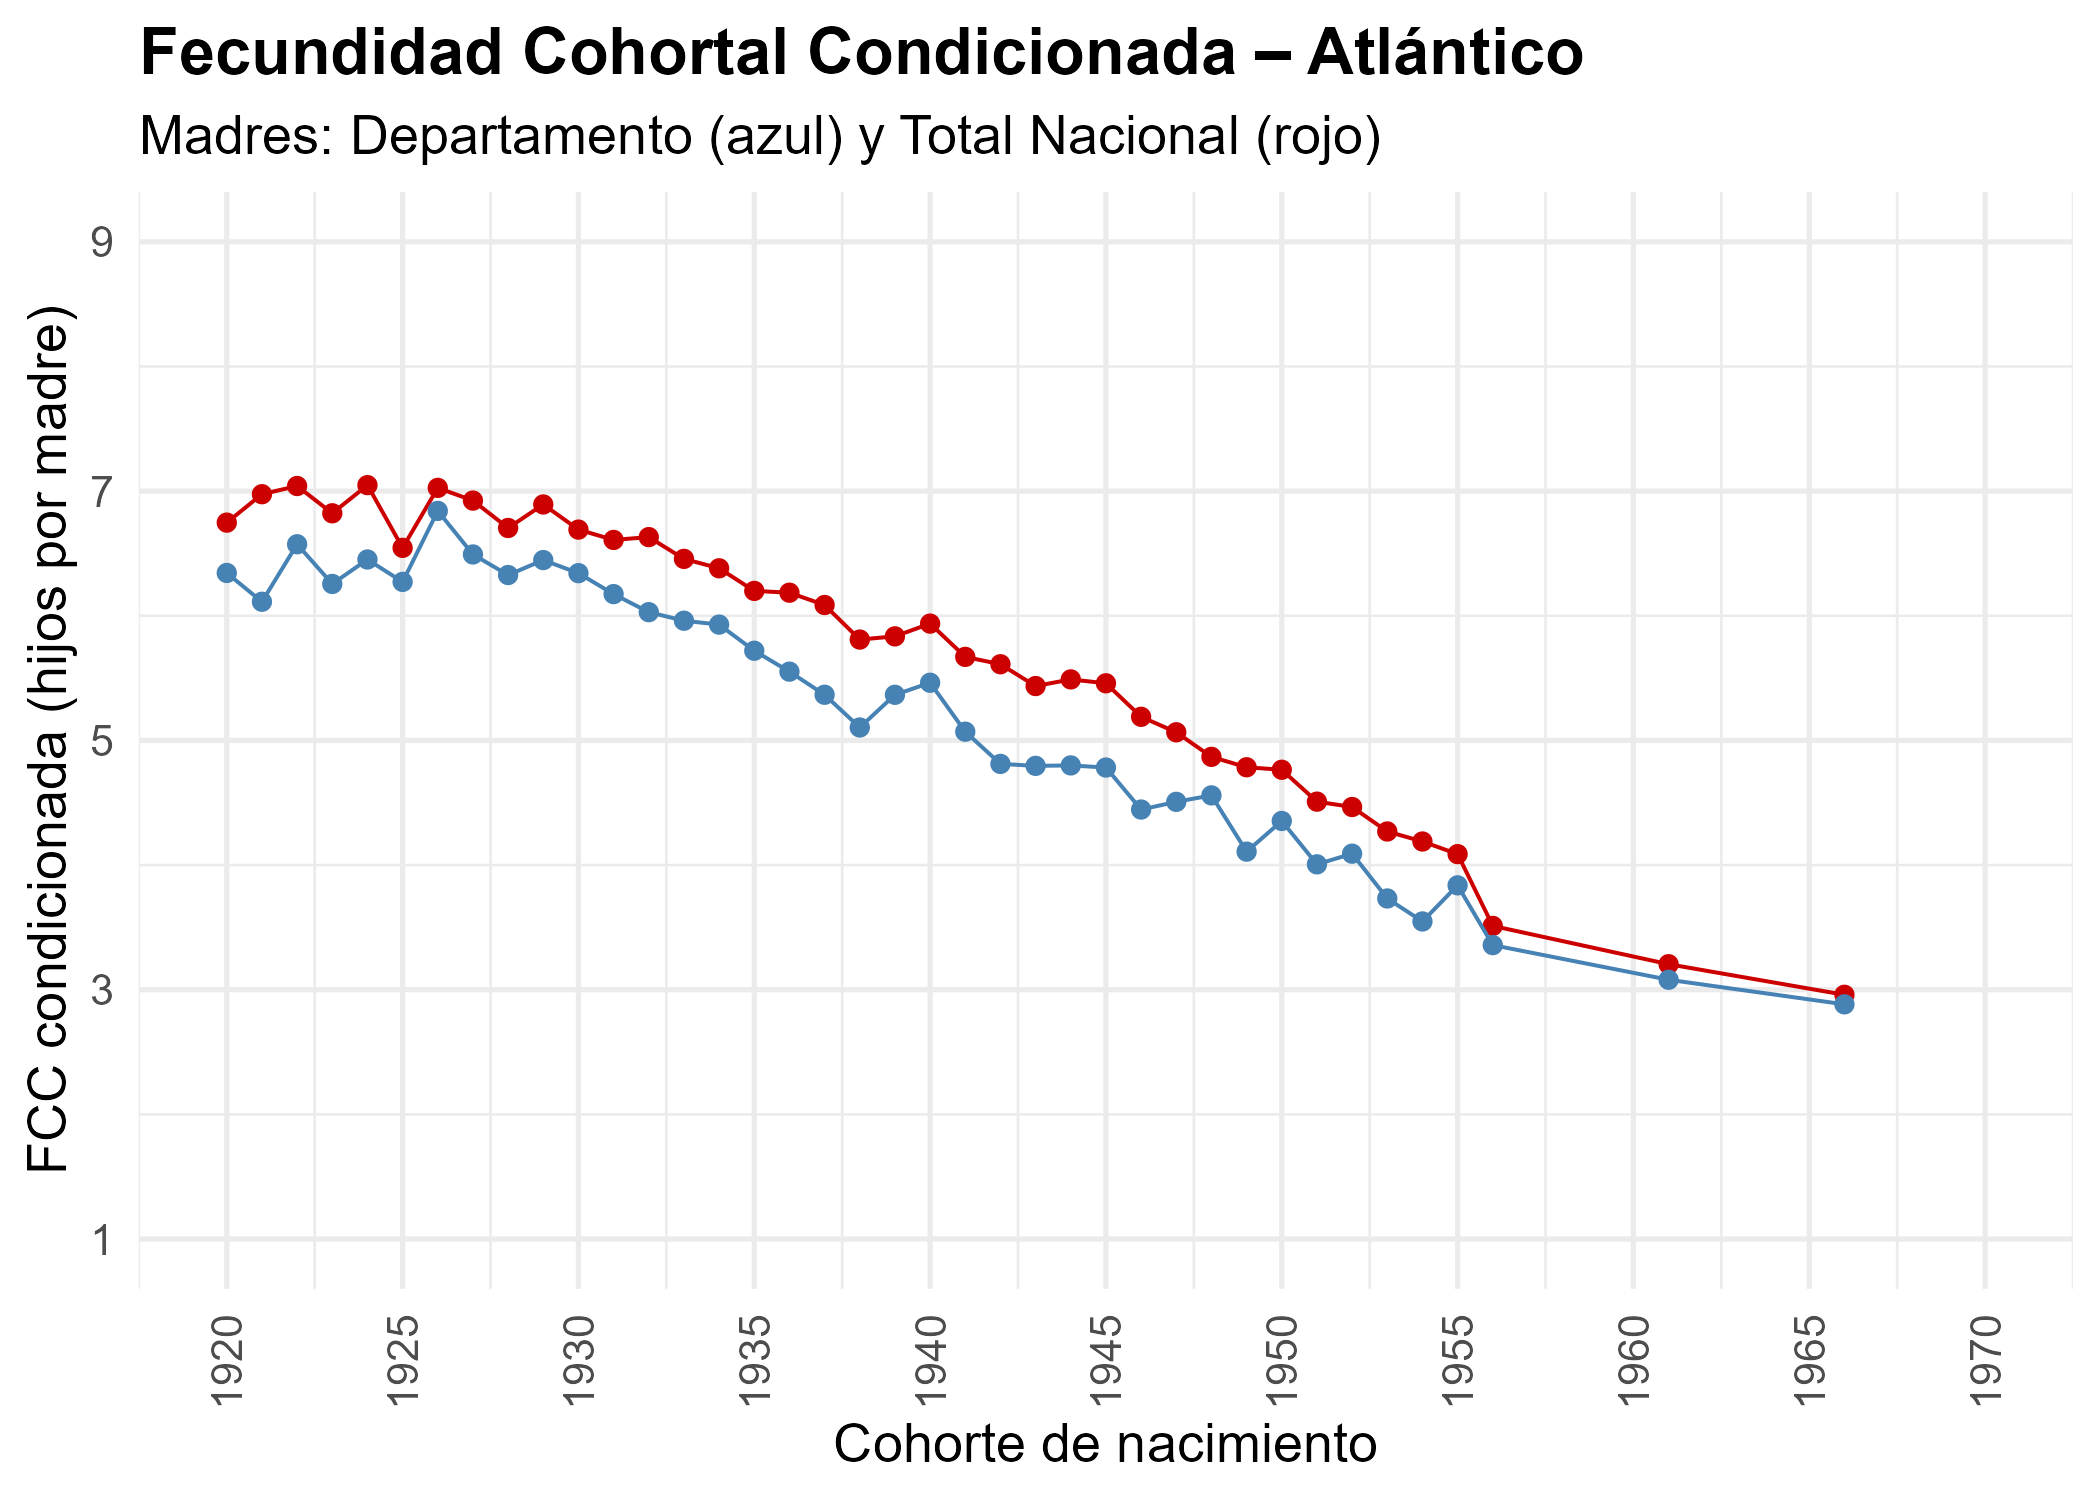
\includegraphics[width=\textwidth]{fcc_departamental/FCC_cond_Atlántico_vs_National.png}
\end{columns}
\end{frame}
\begin{frame}{FCC: Bogotá D.C.}
\begin{columns}
\column{0.5\textwidth}\centering
{\small Todas las mujeres}\\
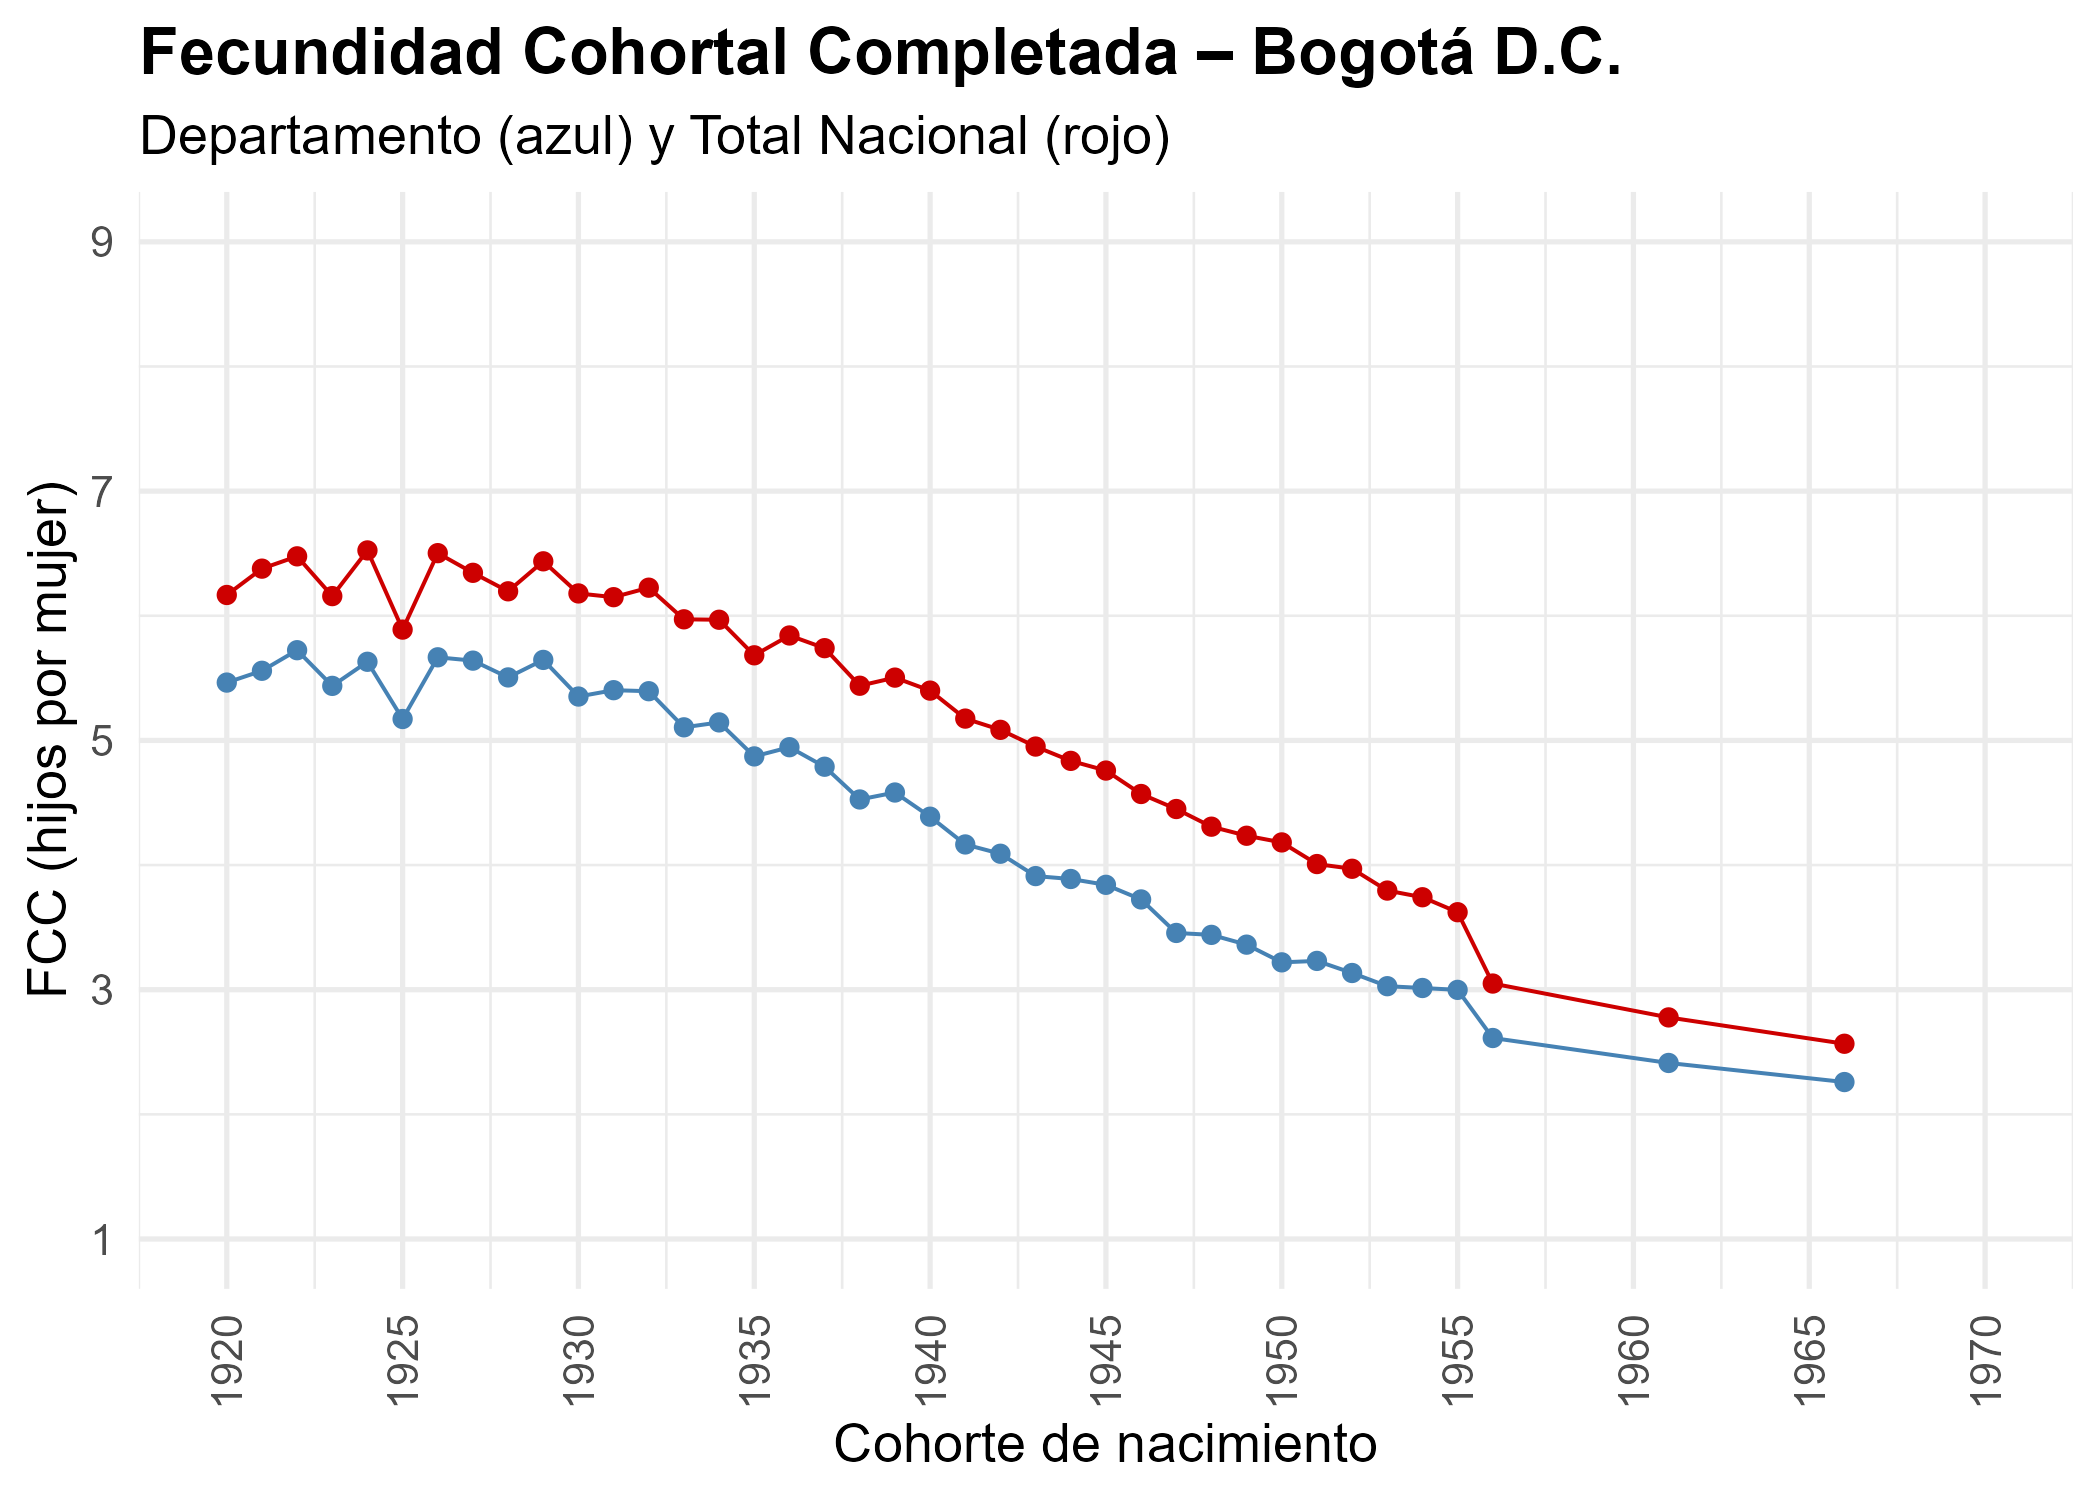
\includegraphics[width=\textwidth]{fcc_departamental/FCC_Bogotá D.C._vs_National.png}
\column{0.5\textwidth}\centering
{\small Condicional (madres)}\\
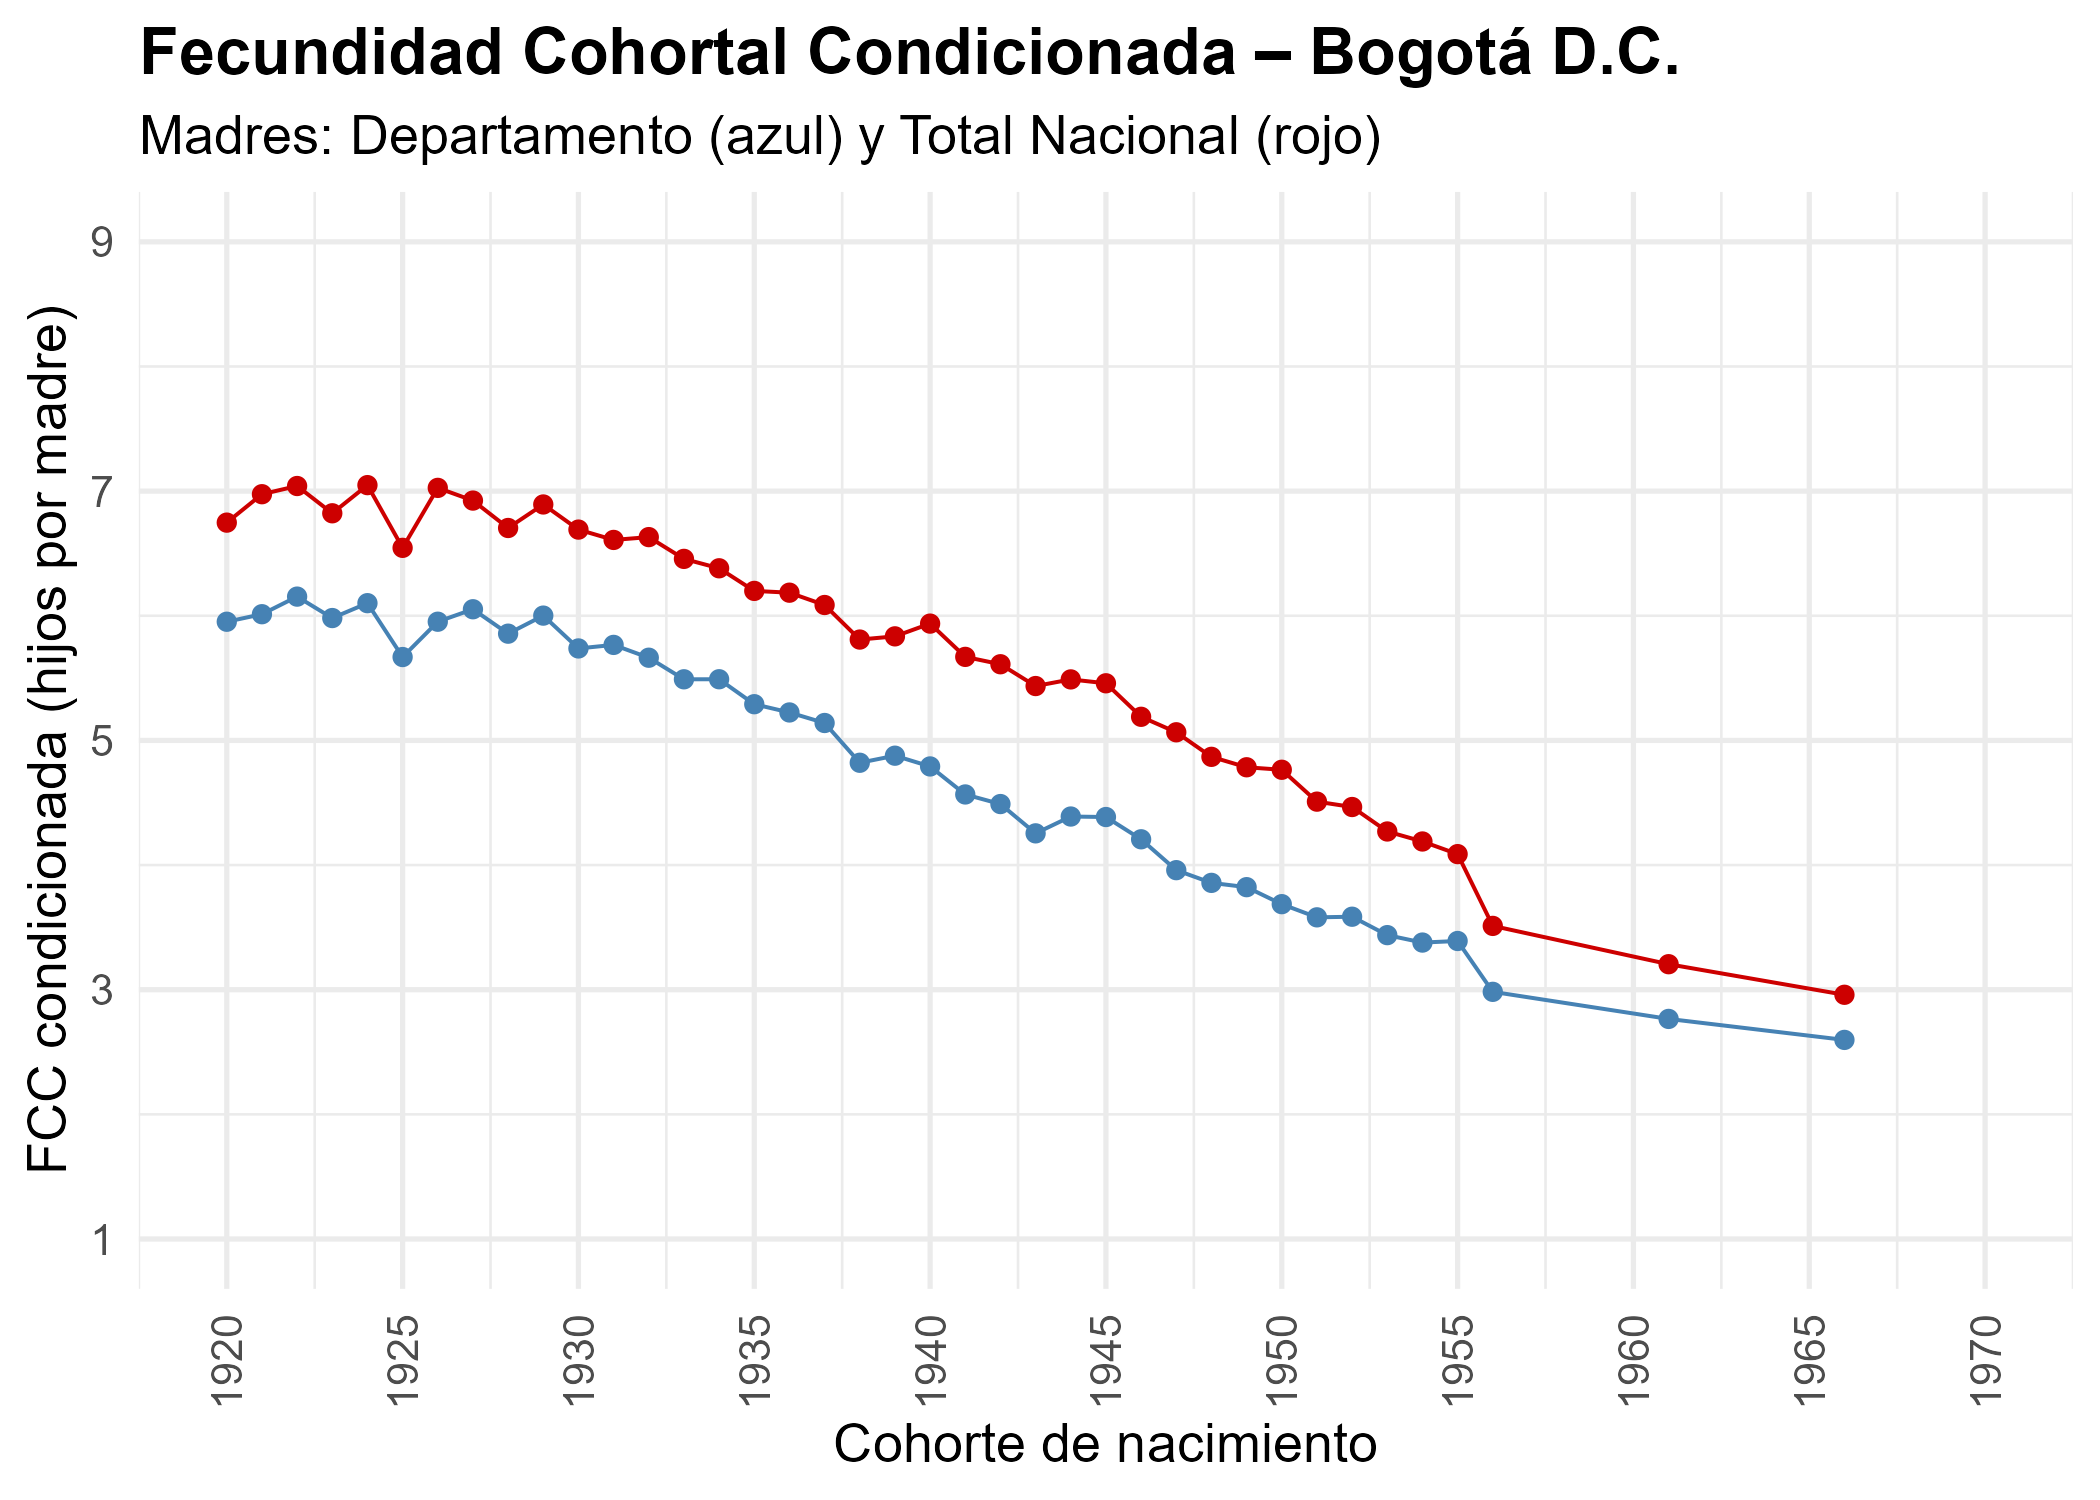
\includegraphics[width=\textwidth]{fcc_departamental/FCC_cond_Bogotá D.C._vs_National.png}
\end{columns}
\end{frame}
\begin{frame}{FCC: Bolívar}
\begin{columns}
\column{0.5\textwidth}\centering
{\small Todas las mujeres}\\
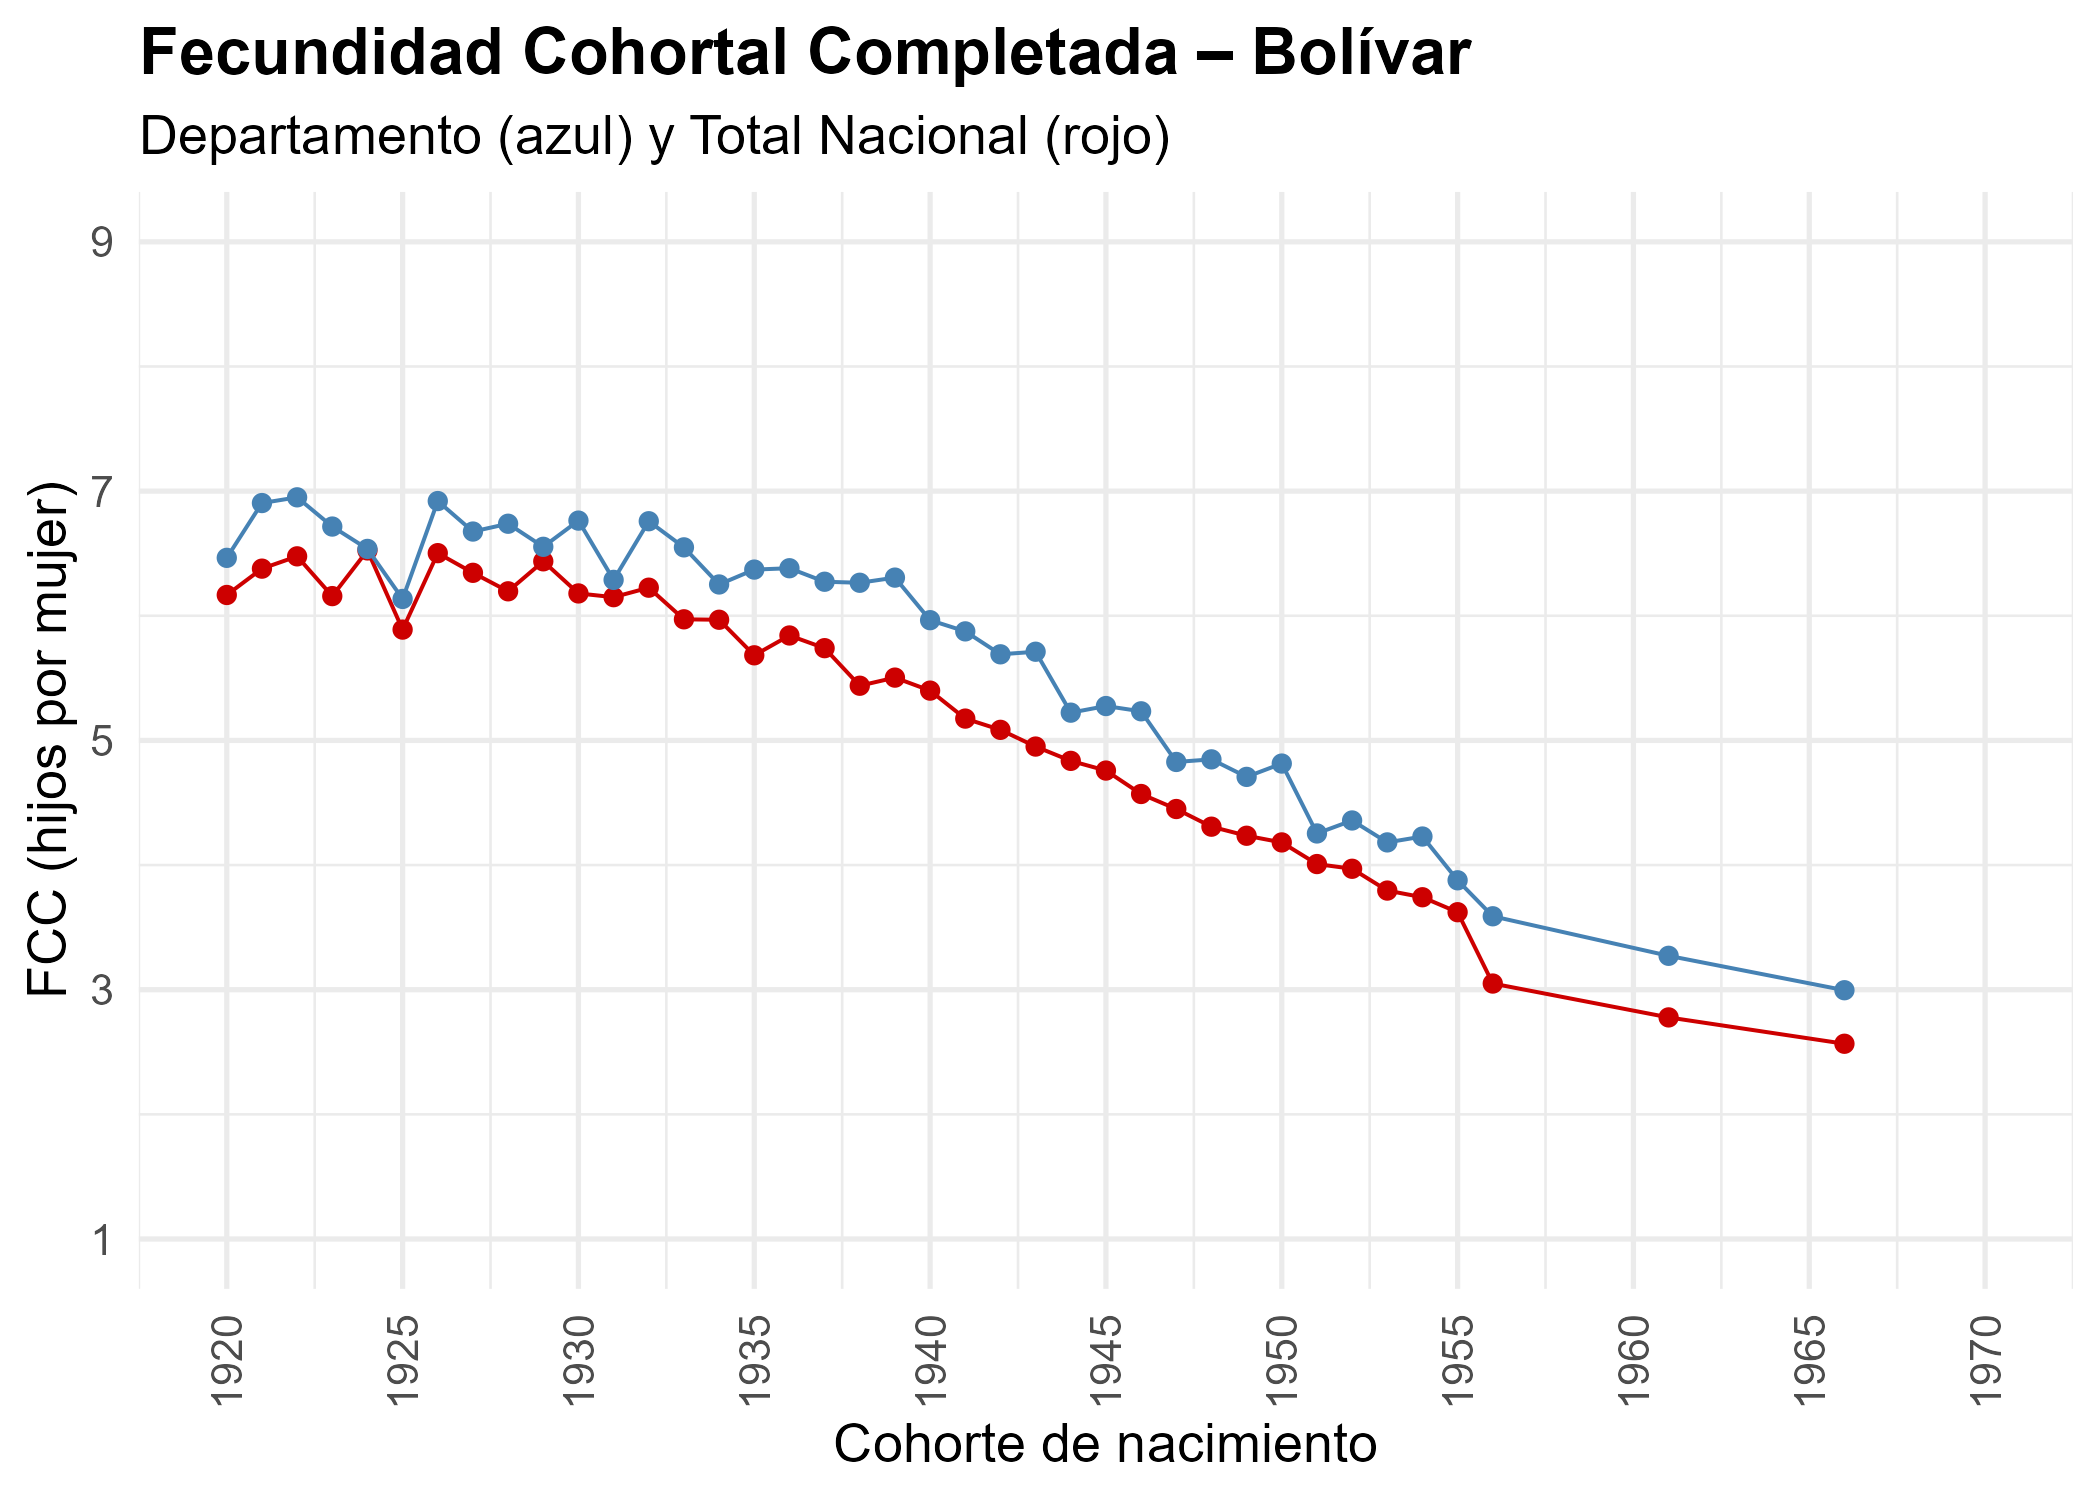
\includegraphics[width=\textwidth]{fcc_departamental/FCC_Bolívar_vs_National.png}
\column{0.5\textwidth}\centering
{\small Condicional (madres)}\\
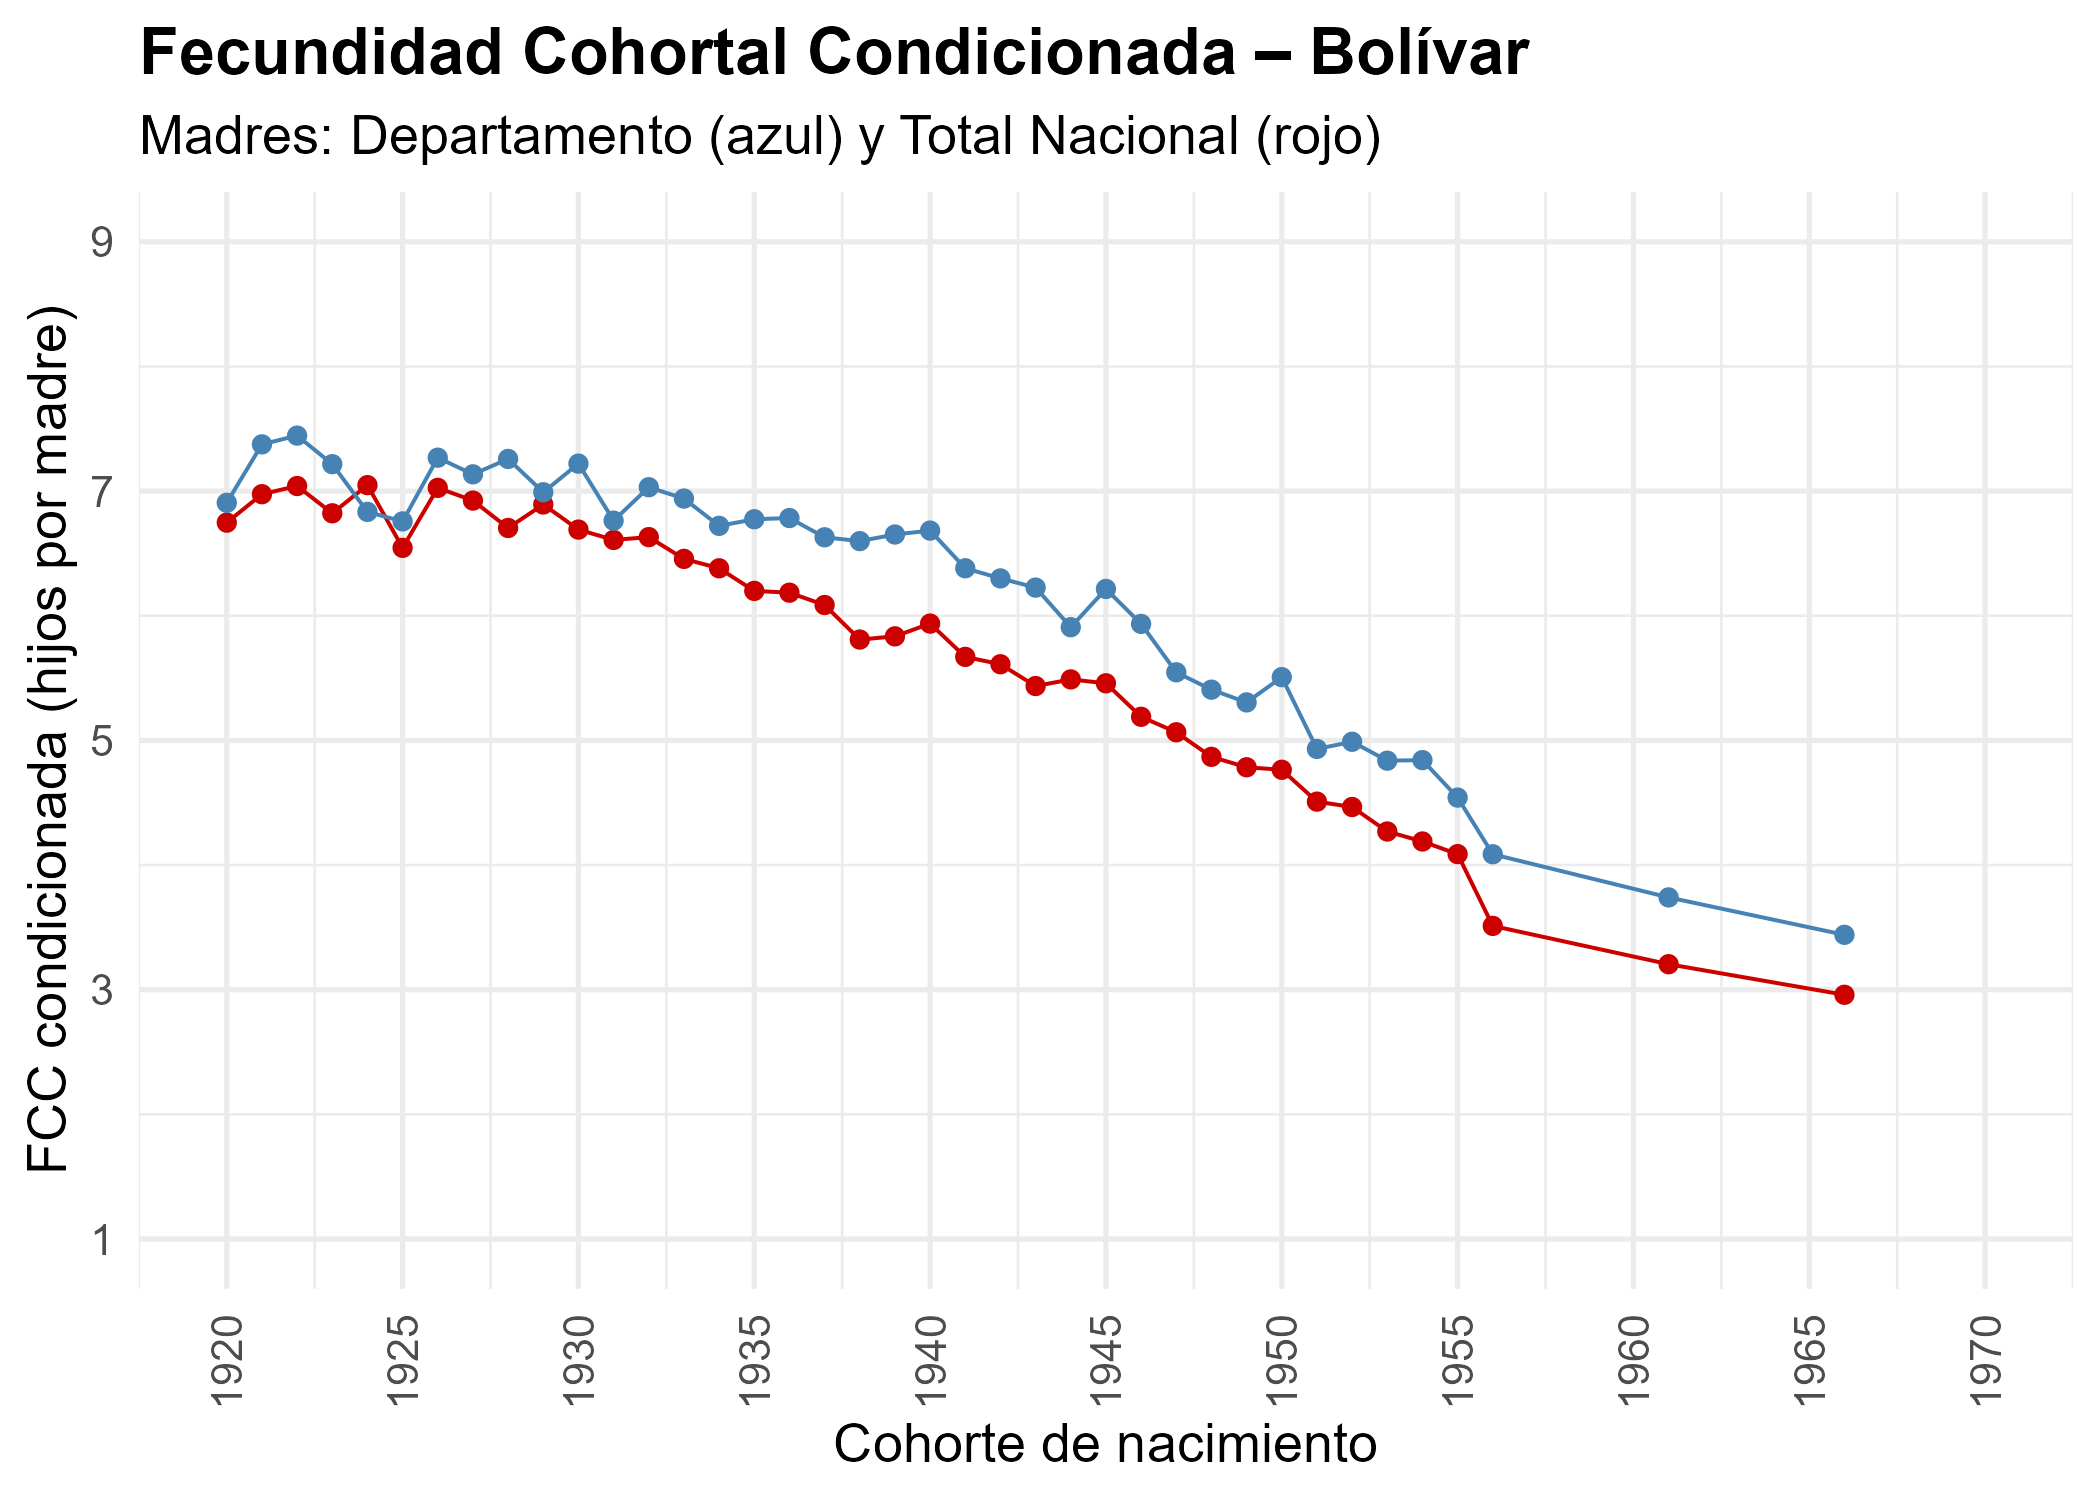
\includegraphics[width=\textwidth]{fcc_departamental/FCC_cond_Bolívar_vs_National.png}
\end{columns}
\end{frame}
\begin{frame}{FCC: Boyacá}
\begin{columns}
\column{0.5\textwidth}\centering
{\small Todas las mujeres}\\
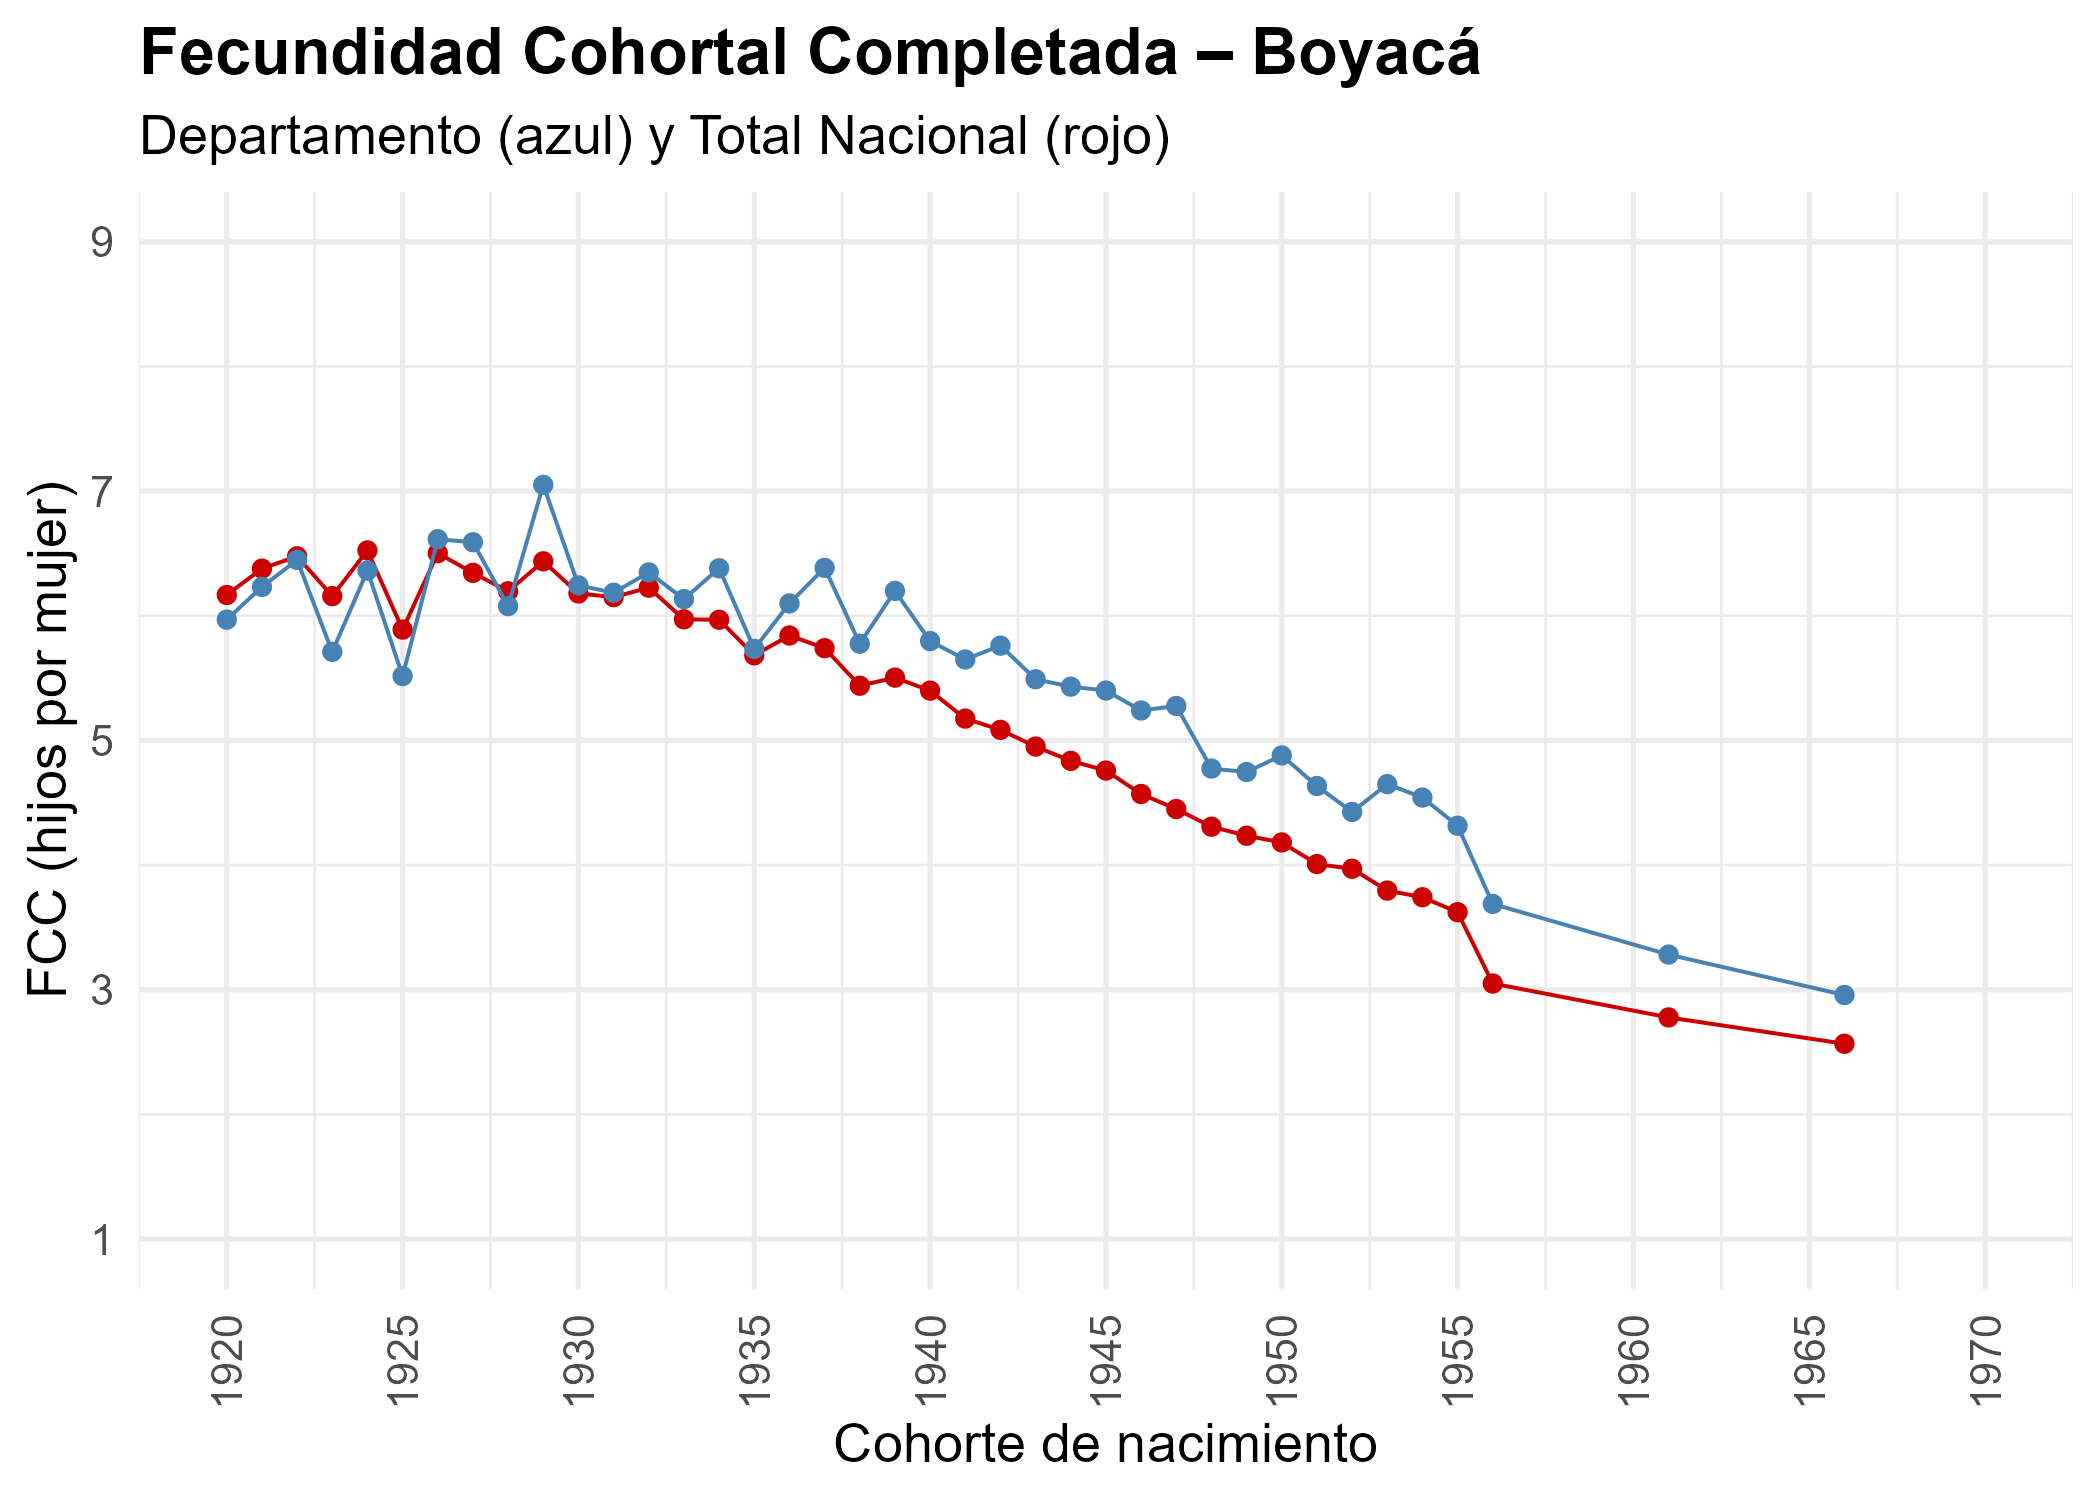
\includegraphics[width=\textwidth]{fcc_departamental/FCC_Boyacá_vs_National.png}
\column{0.5\textwidth}\centering
{\small Condicional (madres)}\\
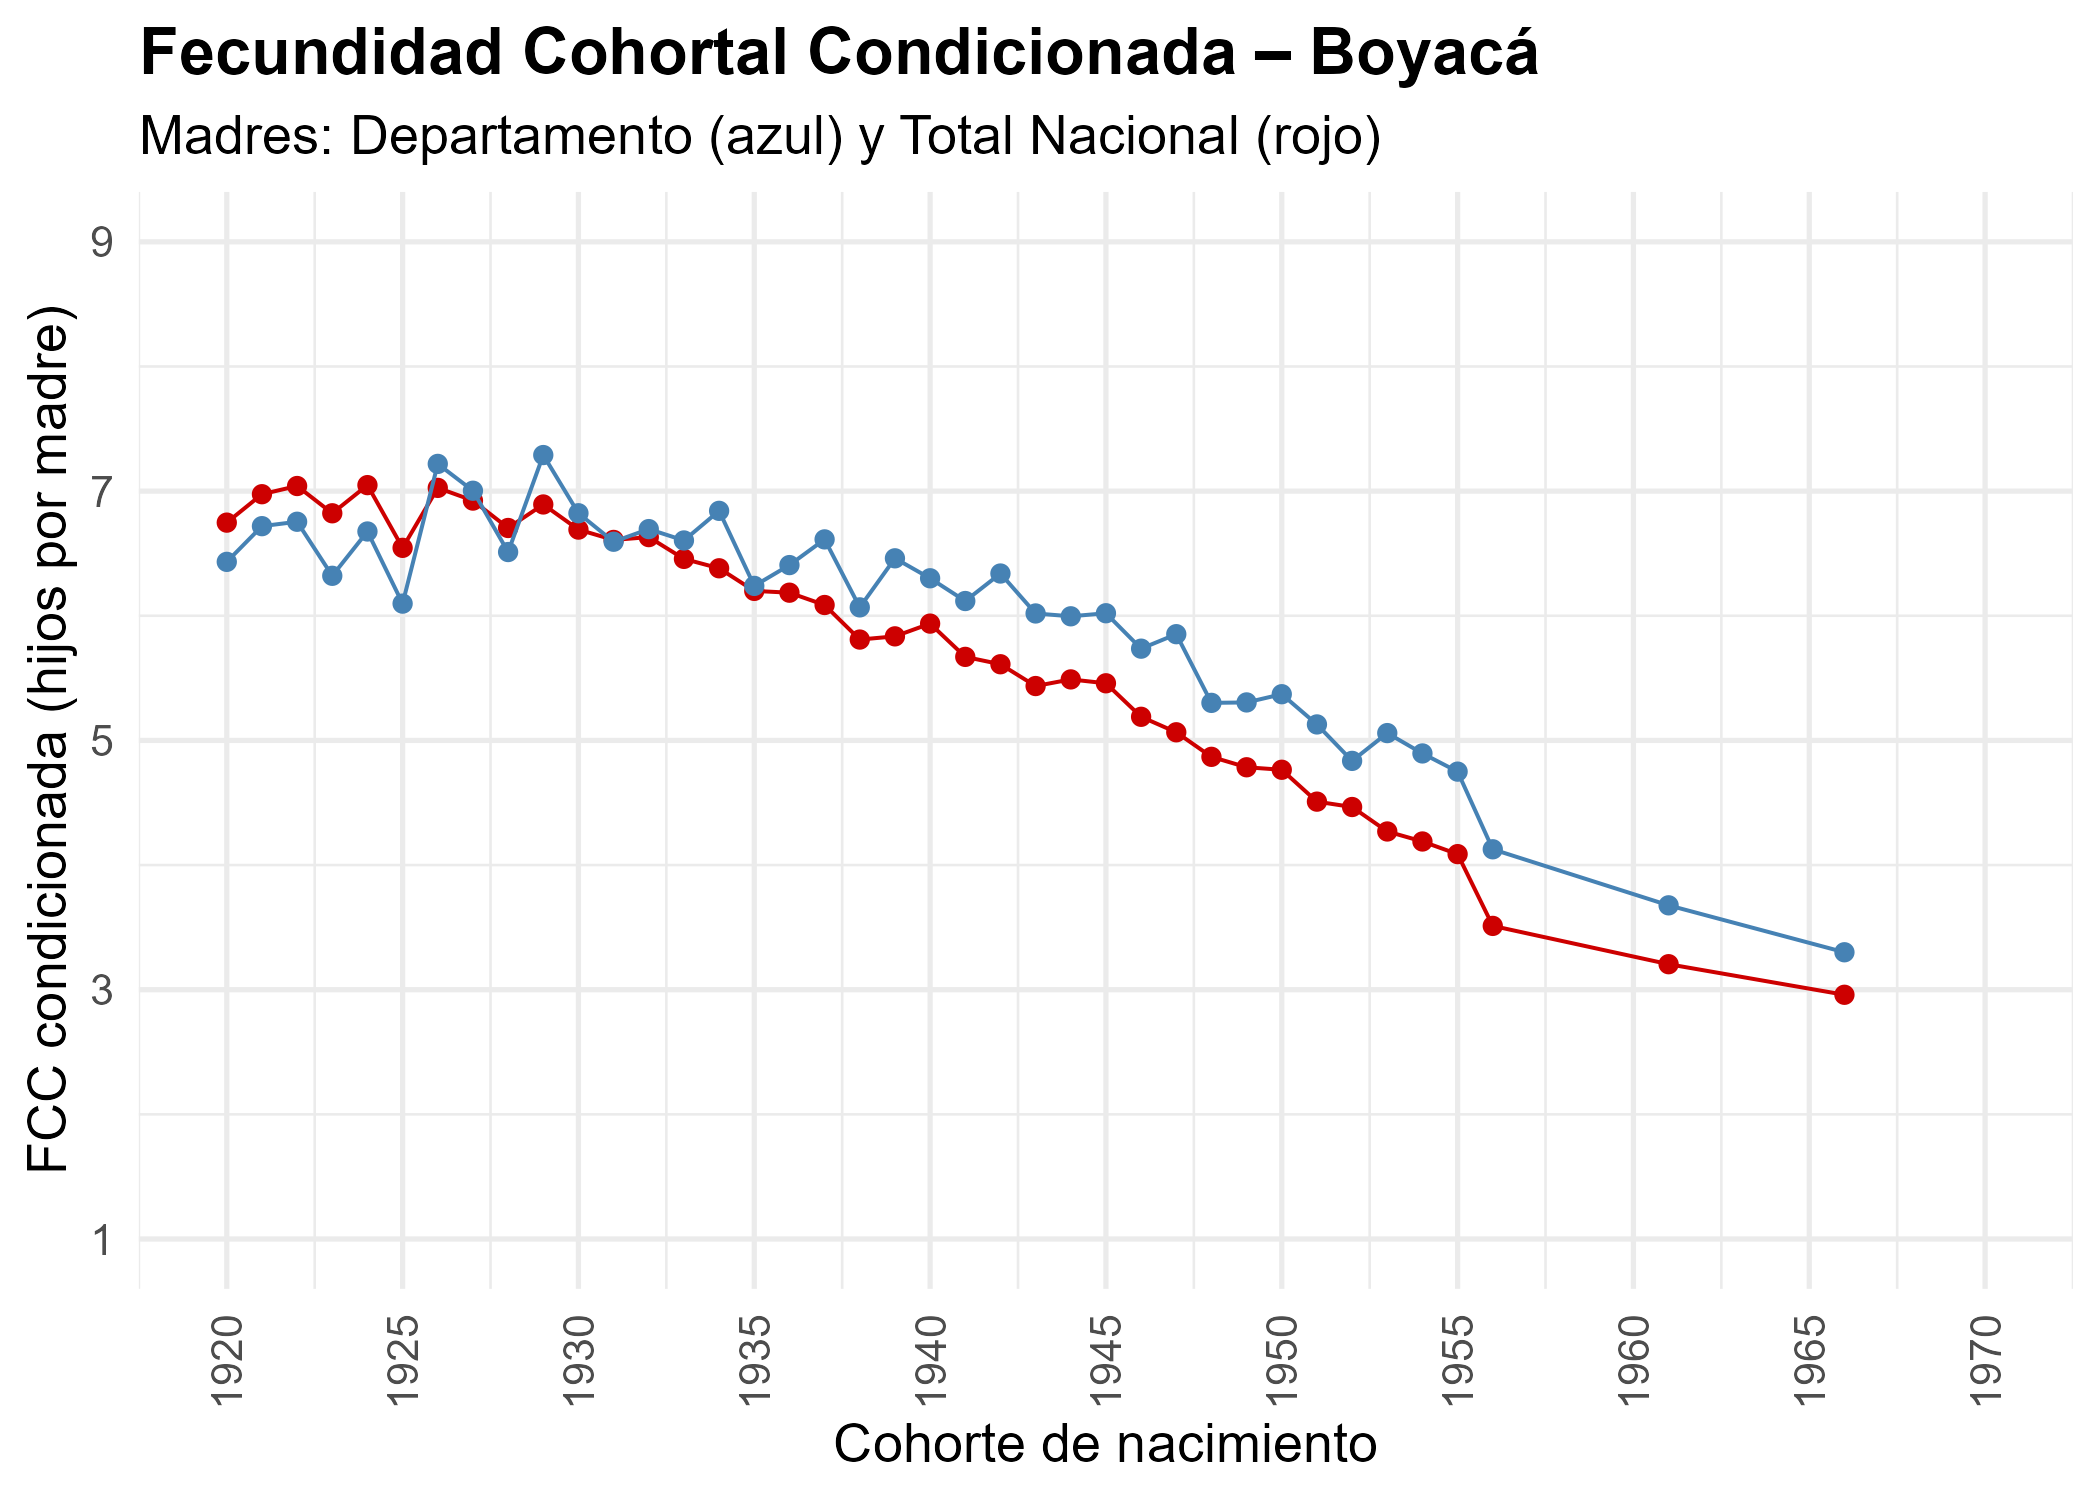
\includegraphics[width=\textwidth]{fcc_departamental/FCC_cond_Boyacá_vs_National.png}
\end{columns}
\end{frame}
\begin{frame}{FCC: Caldas}
\begin{columns}
\column{0.5\textwidth}\centering
{\small Todas las mujeres}\\
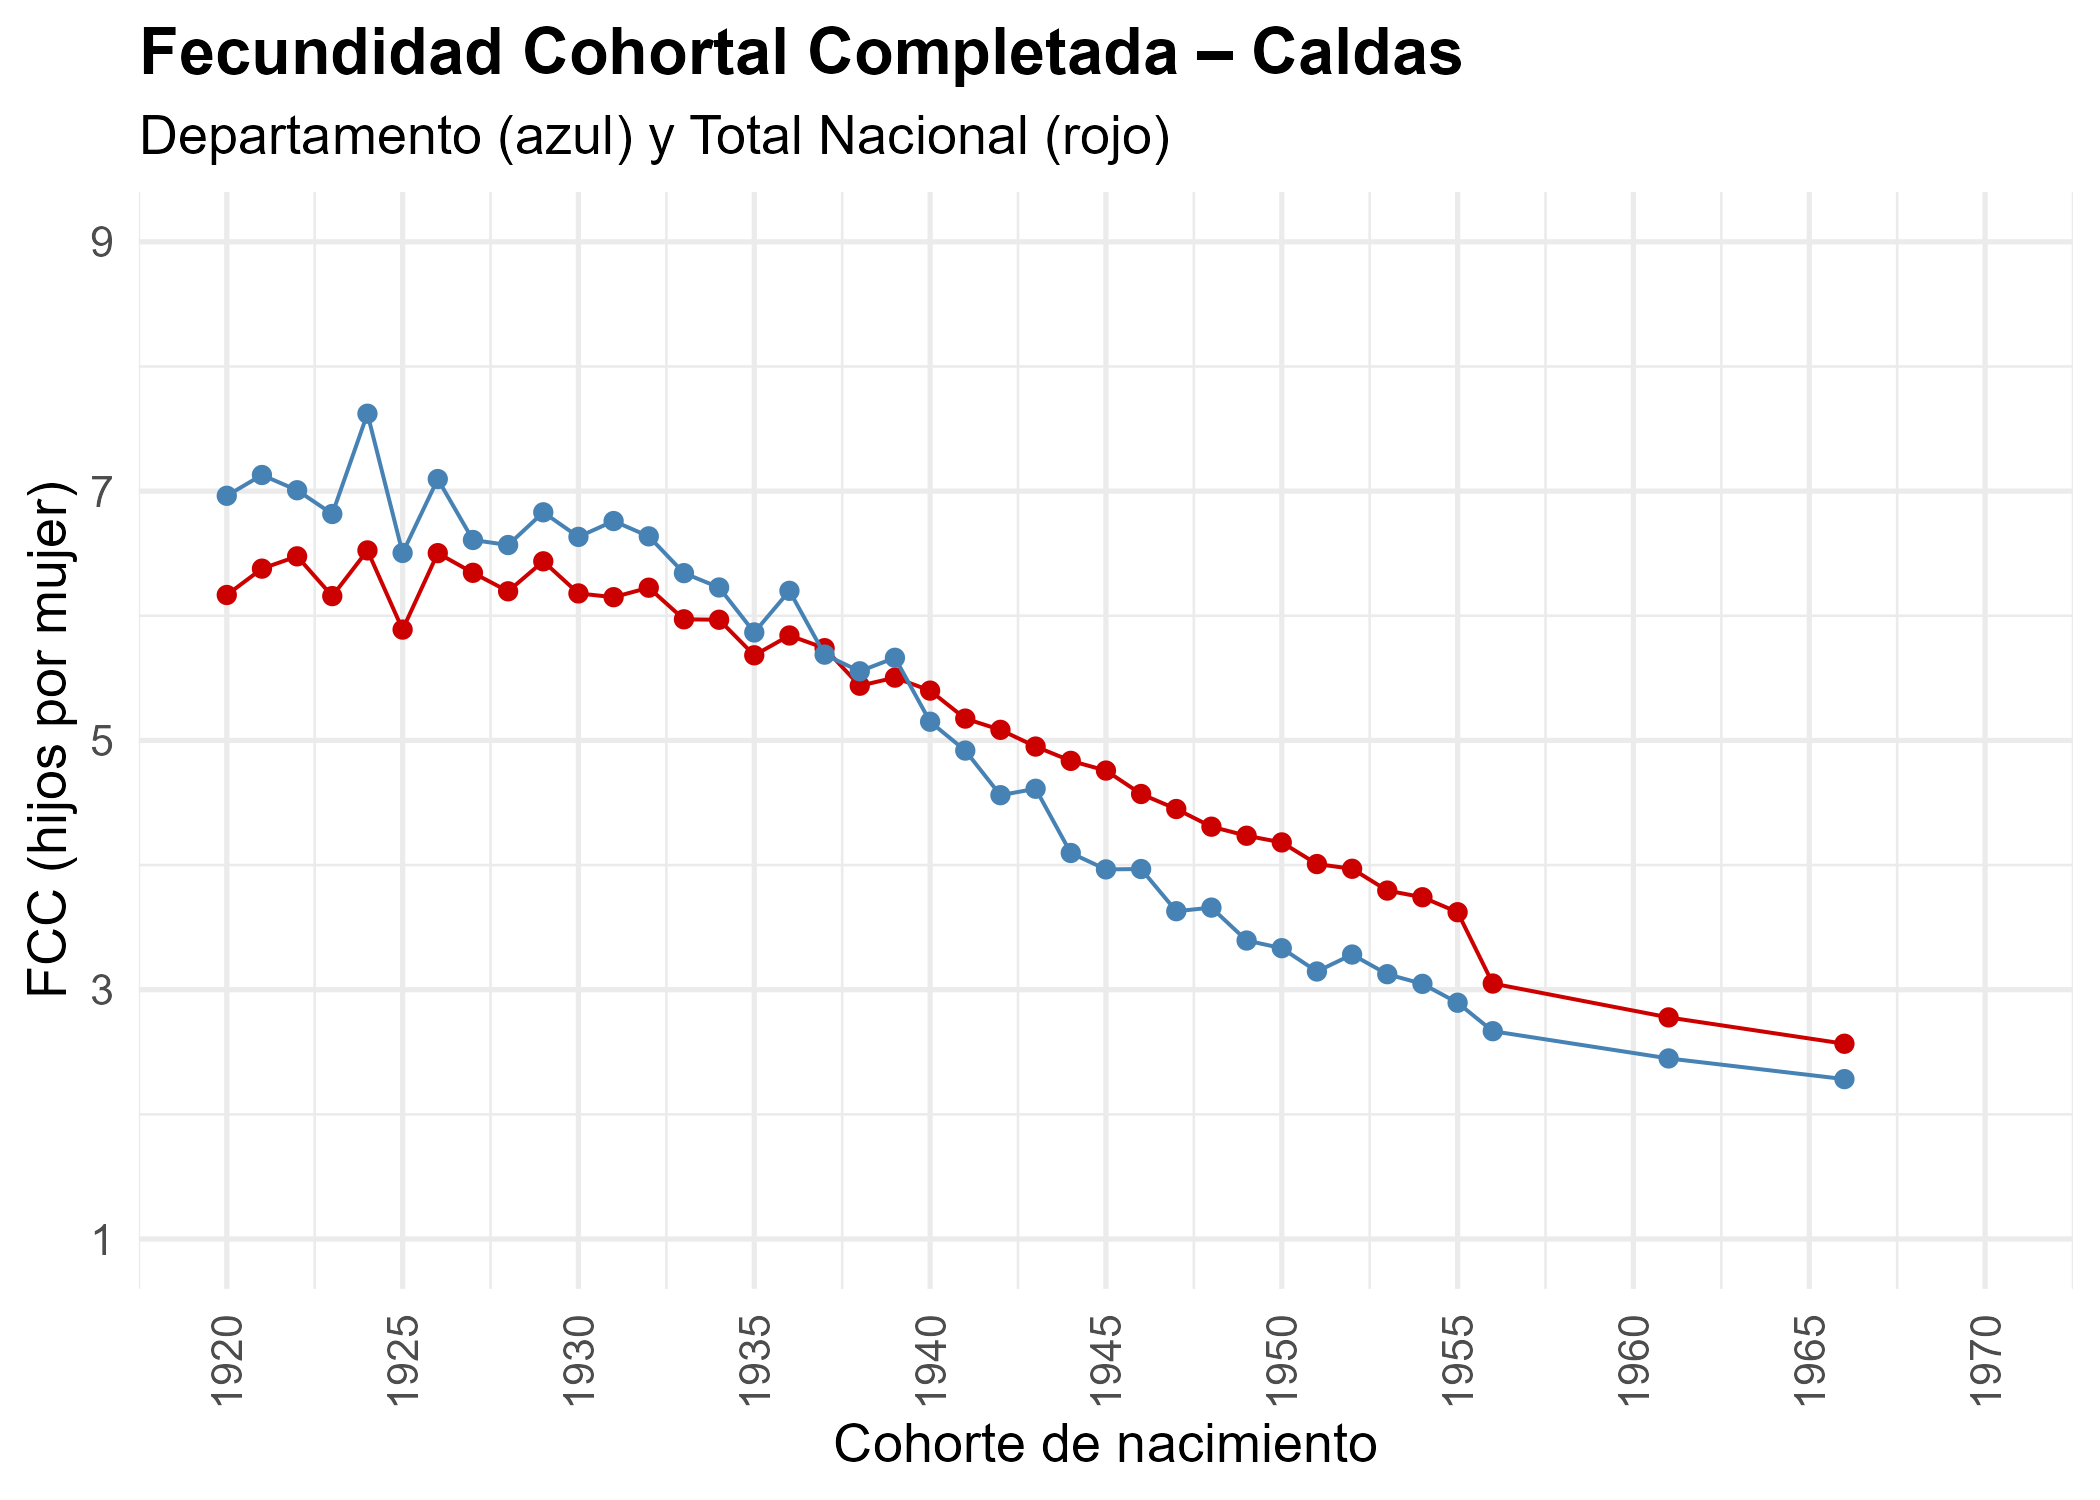
\includegraphics[width=\textwidth]{fcc_departamental/FCC_Caldas_vs_National.png}
\column{0.5\textwidth}\centering
{\small Condicional (madres)}\\
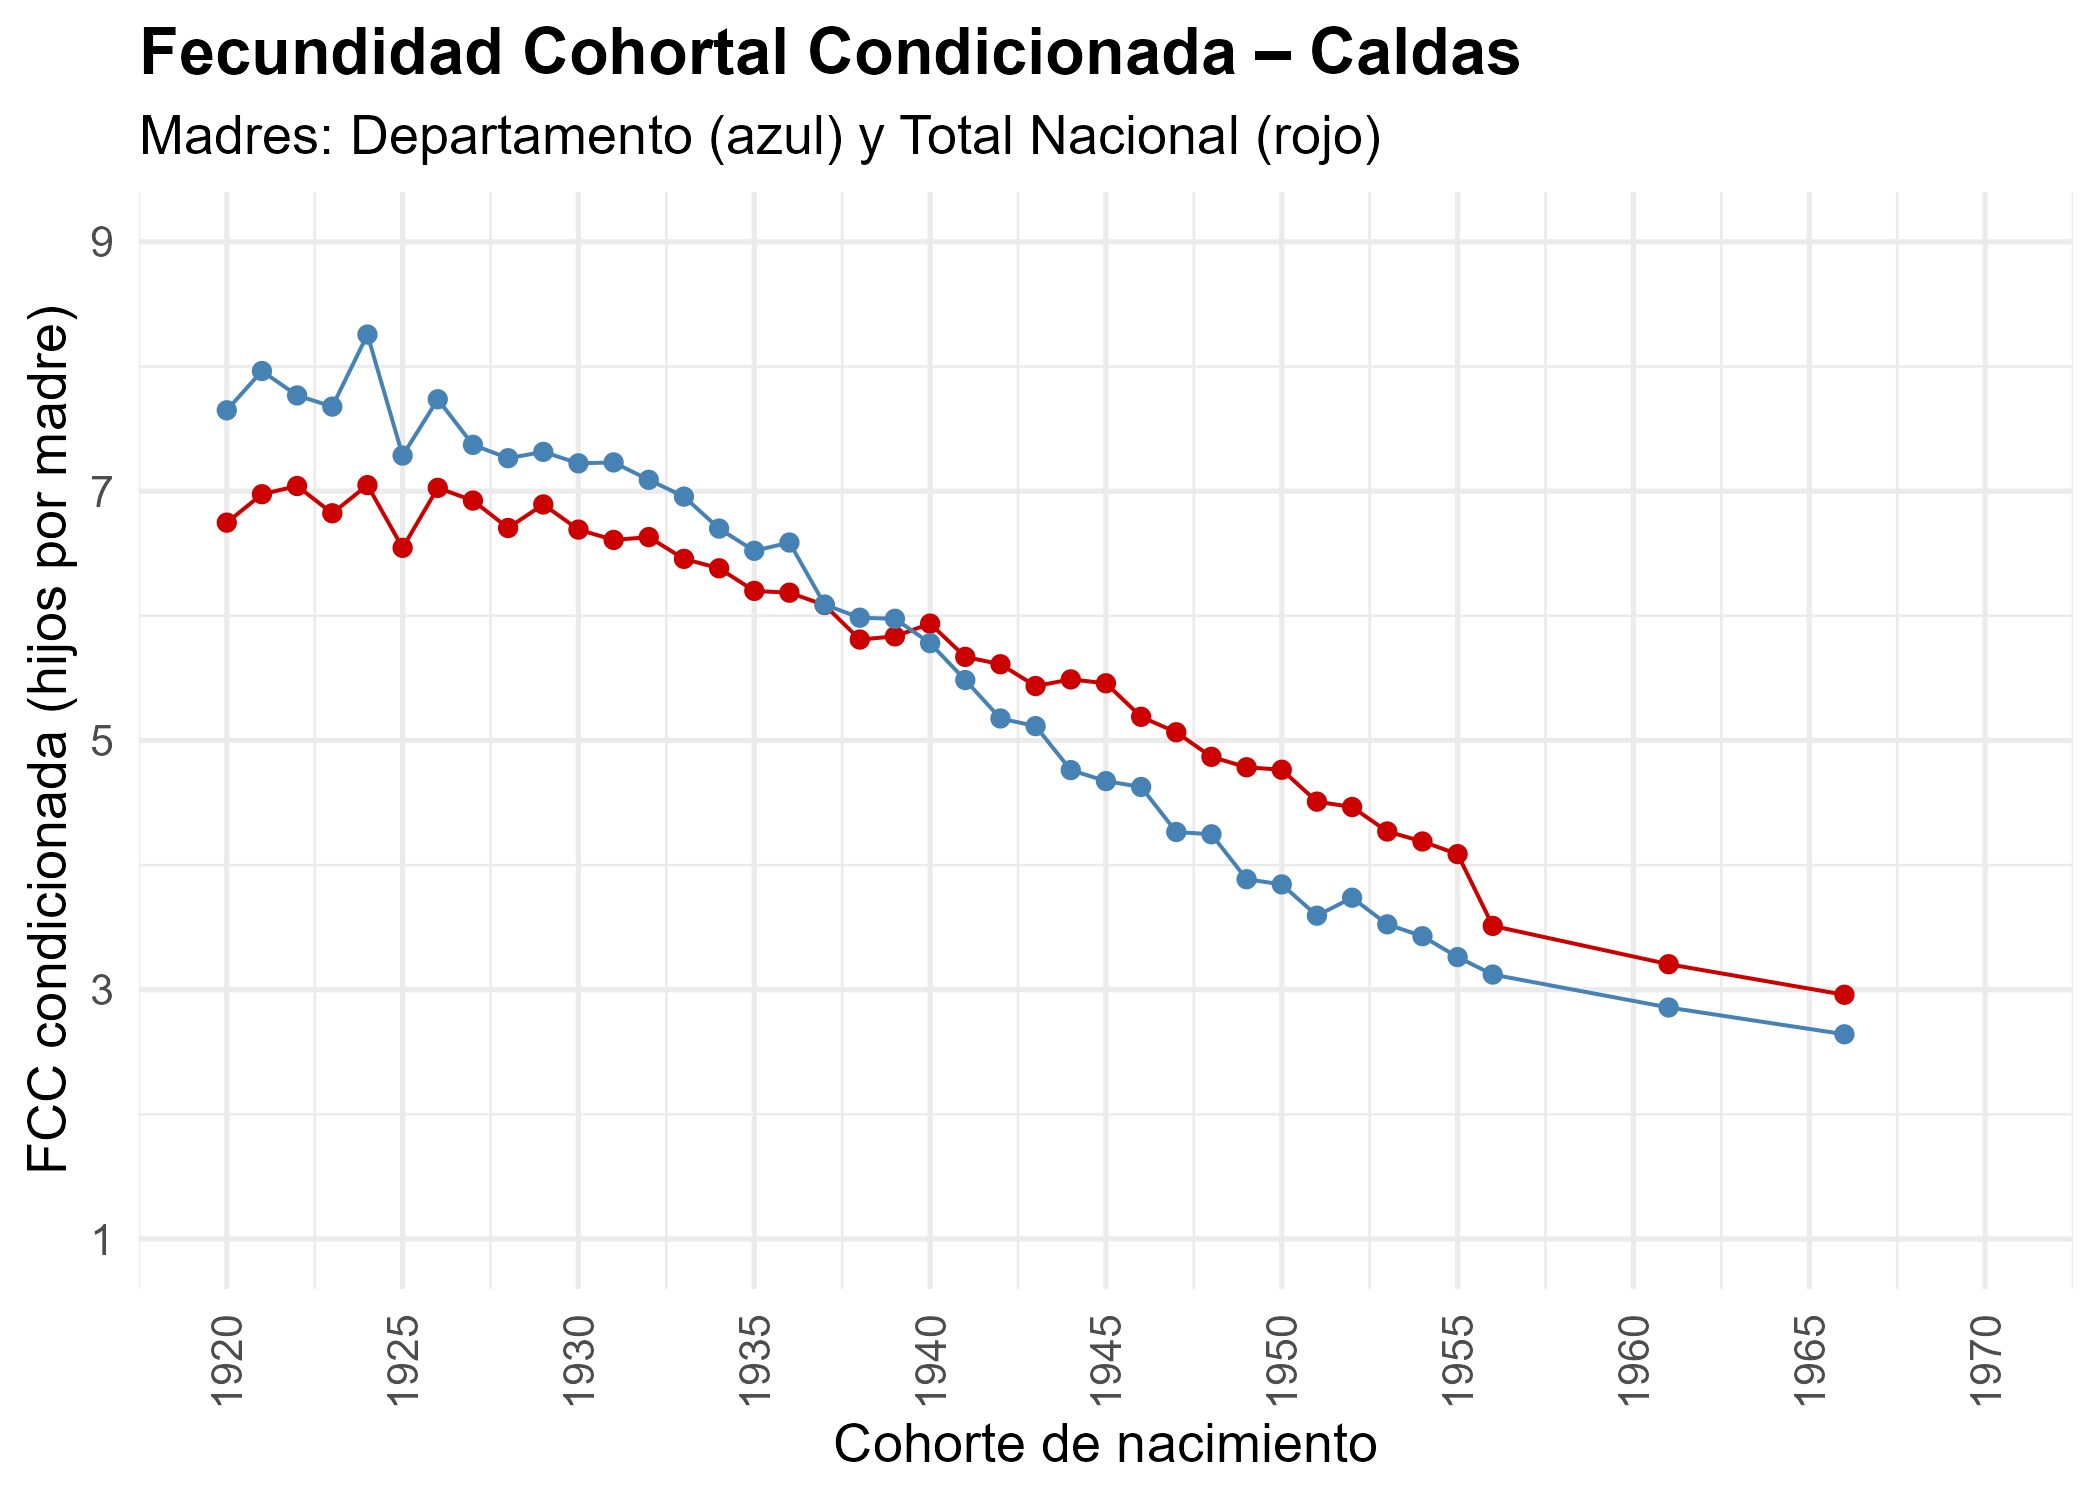
\includegraphics[width=\textwidth]{fcc_departamental/FCC_cond_Caldas_vs_National.png}
\end{columns}
\end{frame}
\begin{frame}{FCC: Caquetá}
\begin{columns}
\column{0.5\textwidth}\centering
{\small Todas las mujeres}\\
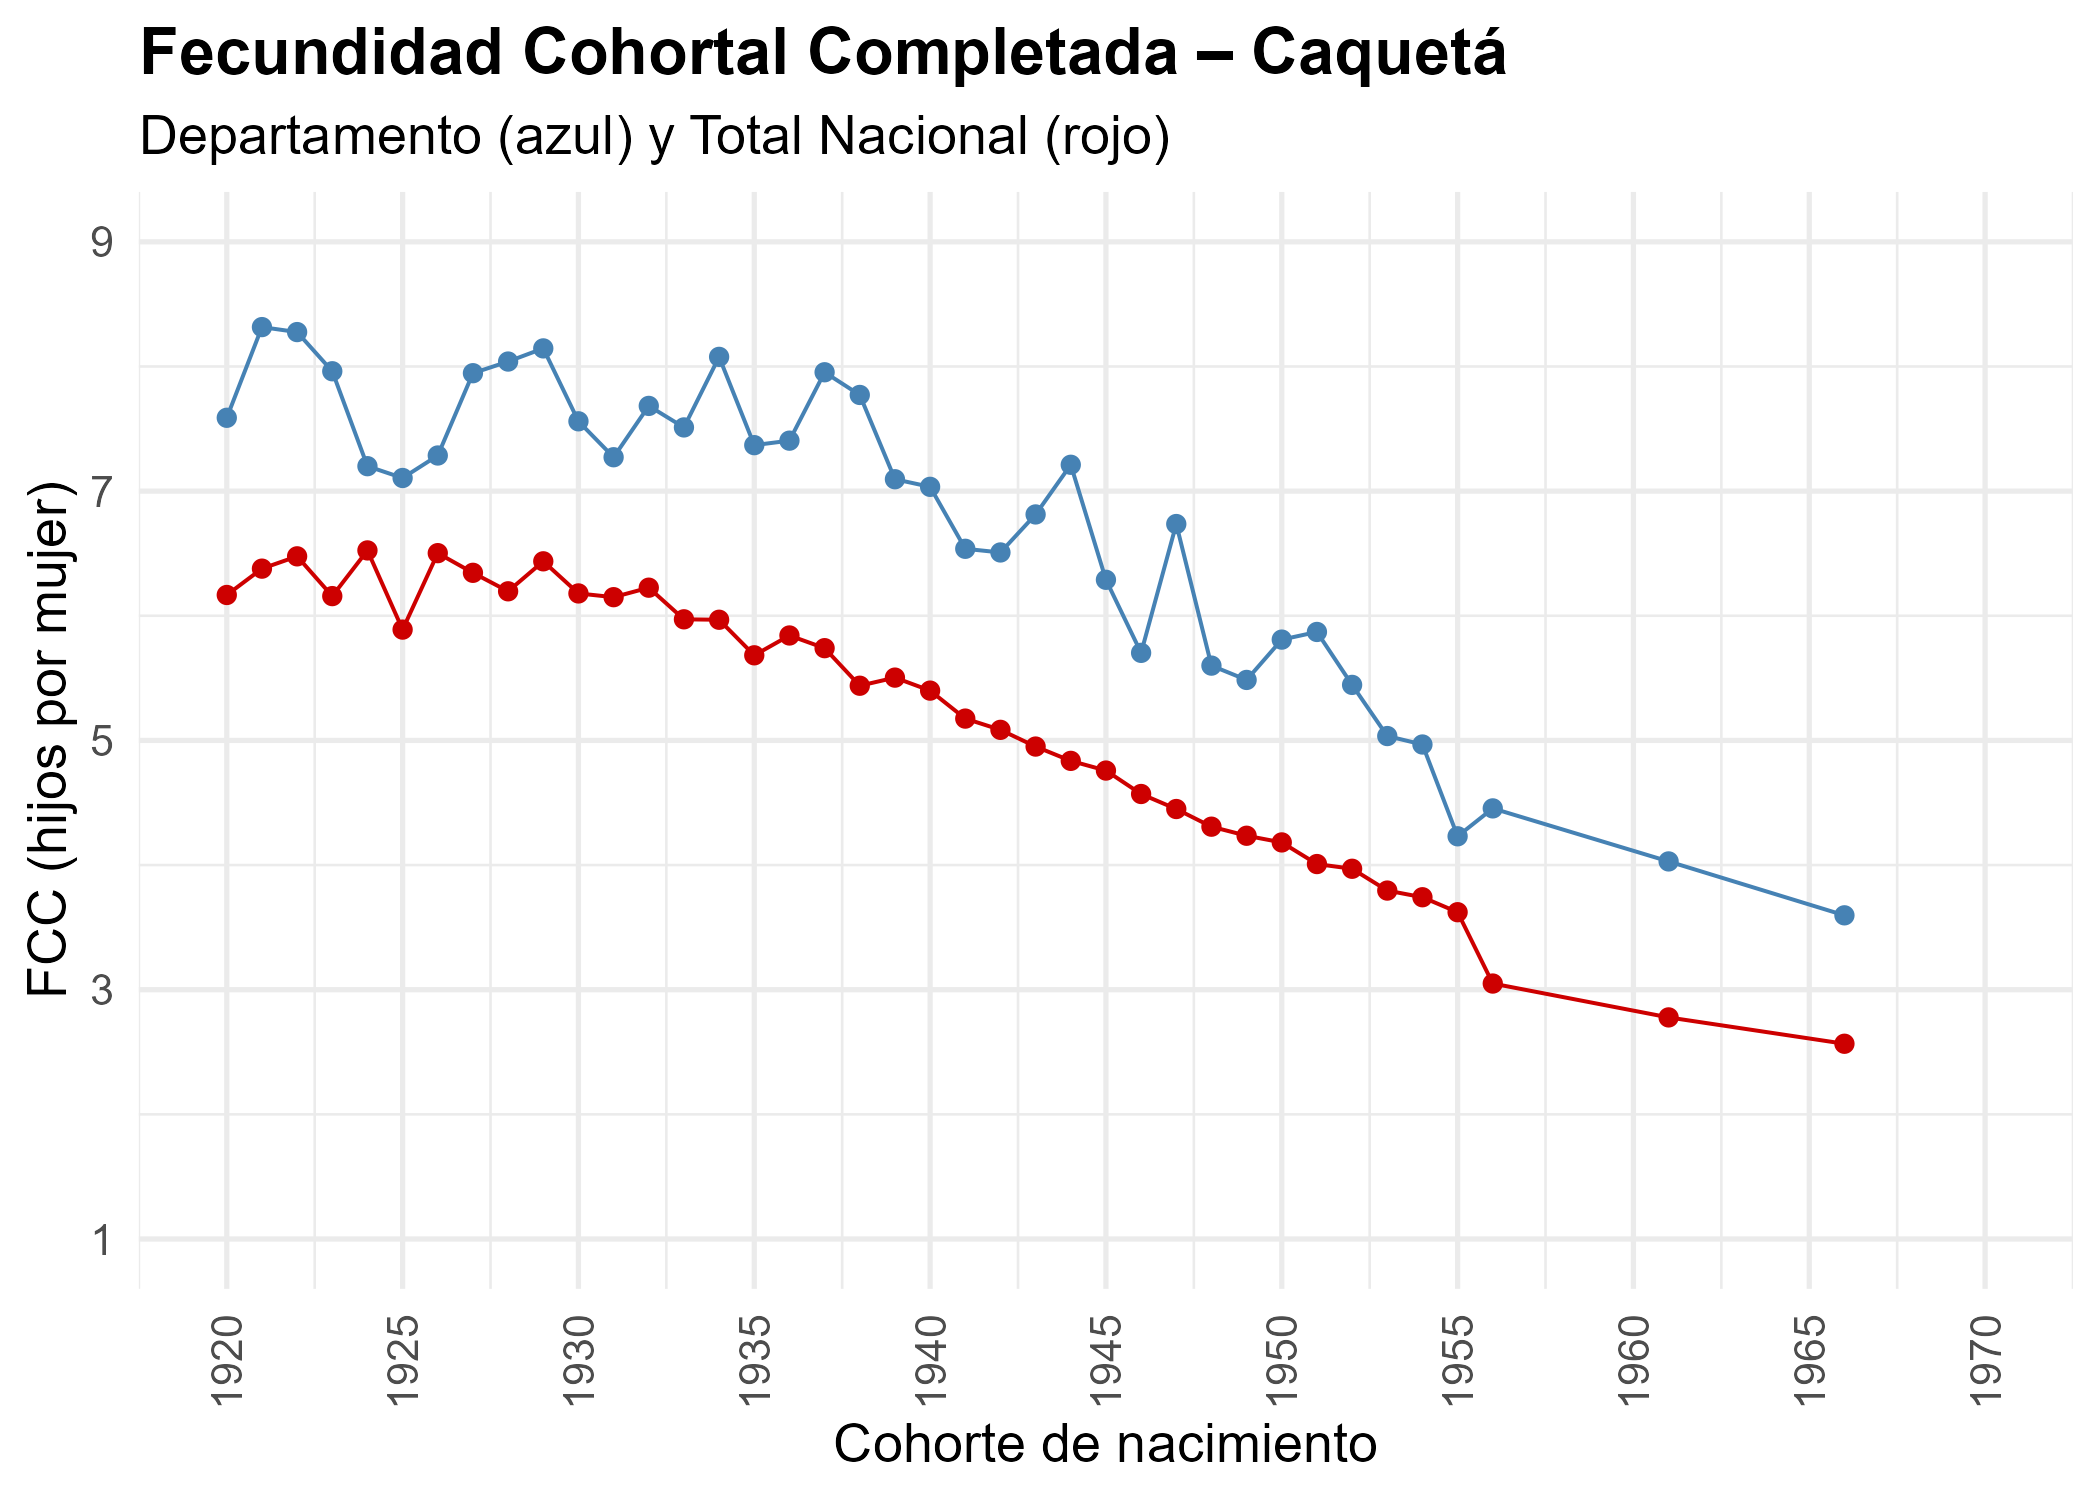
\includegraphics[width=\textwidth]{fcc_departamental/FCC_Caquetá_vs_National.png}
\column{0.5\textwidth}\centering
{\small Condicional (madres)}\\
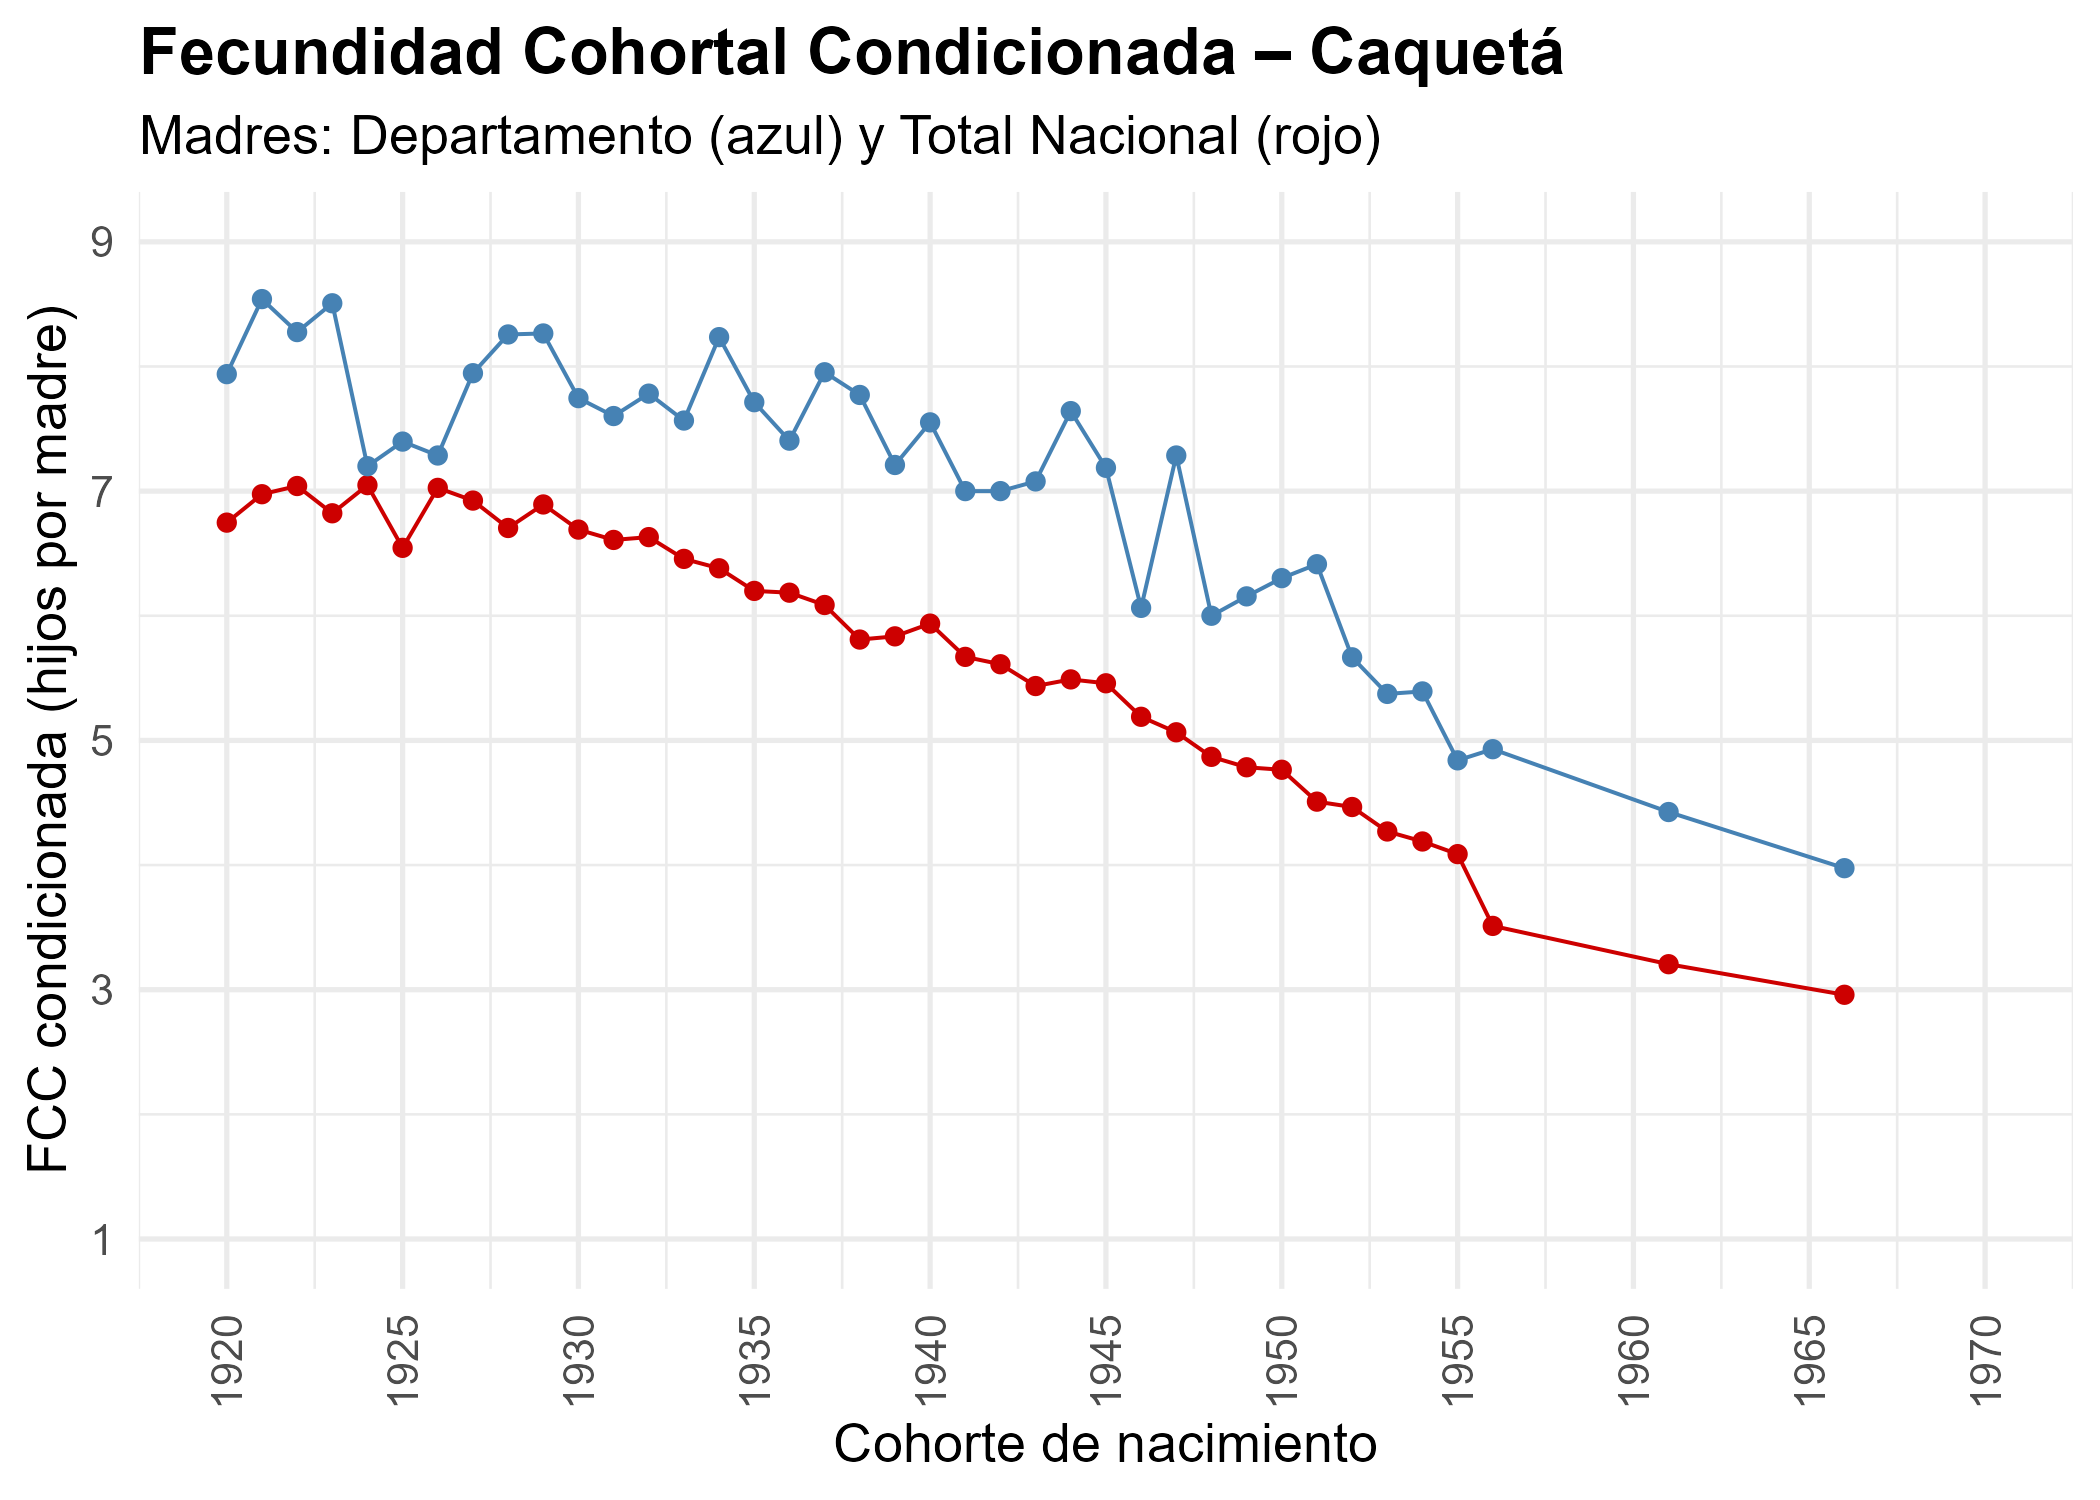
\includegraphics[width=\textwidth]{fcc_departamental/FCC_cond_Caquetá_vs_National.png}
\end{columns}
\end{frame}
\begin{frame}{FCC: Cauca}
\begin{columns}
\column{0.5\textwidth}\centering
{\small Todas las mujeres}\\
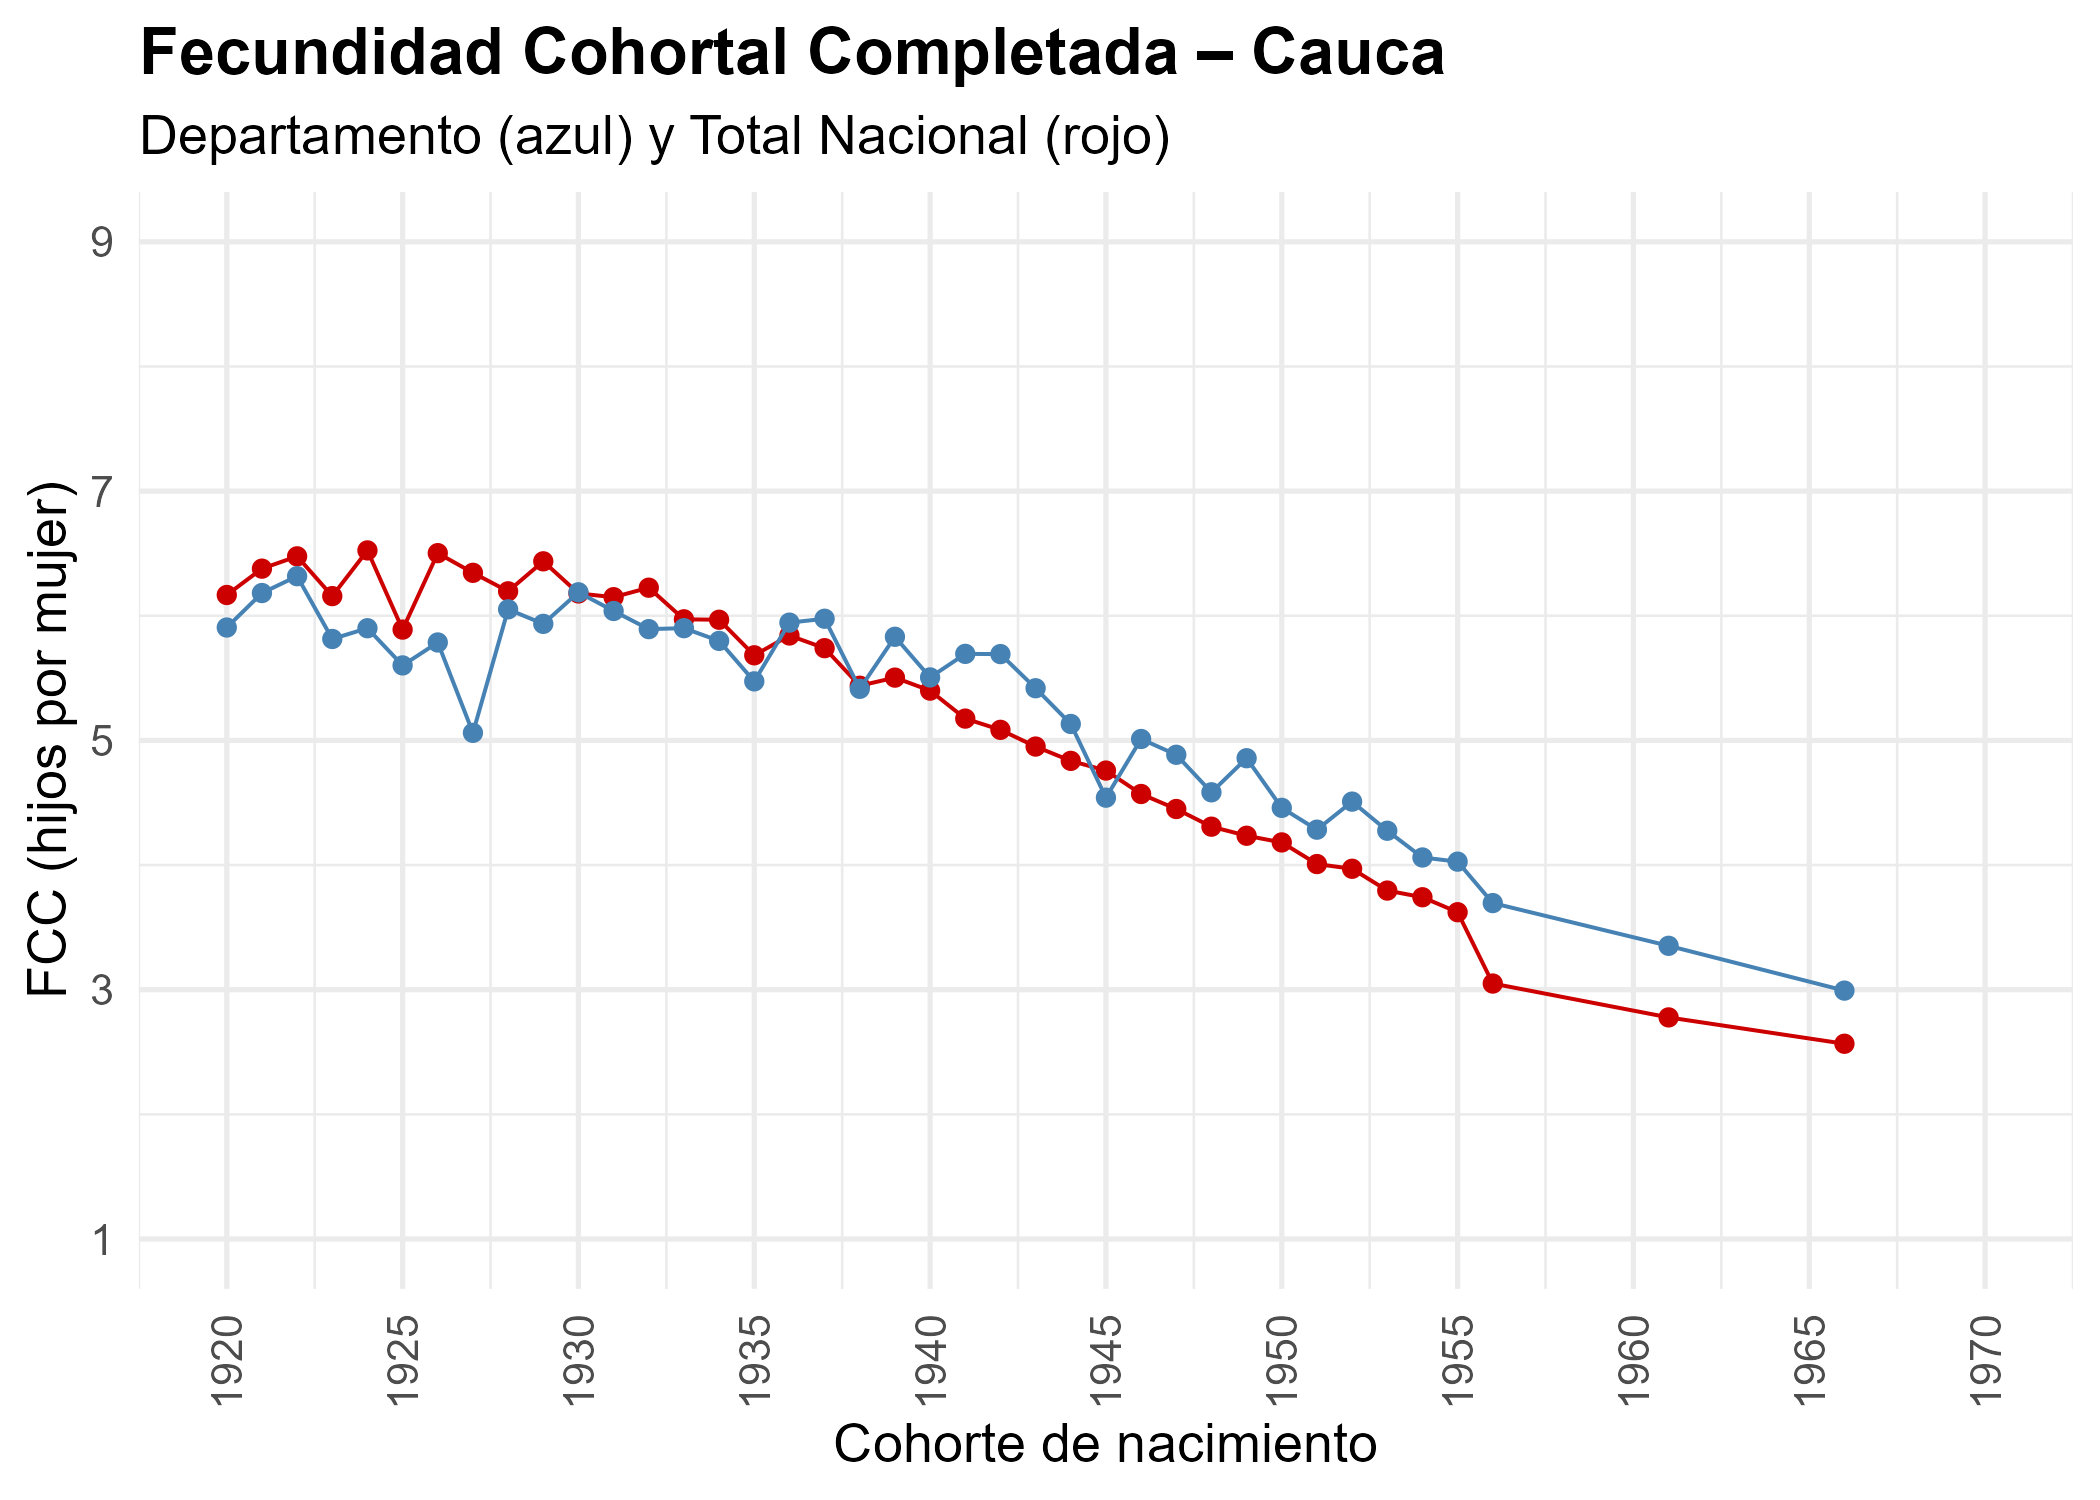
\includegraphics[width=\textwidth]{fcc_departamental/FCC_Cauca_vs_National.png}
\column{0.5\textwidth}\centering
{\small Condicional (madres)}\\
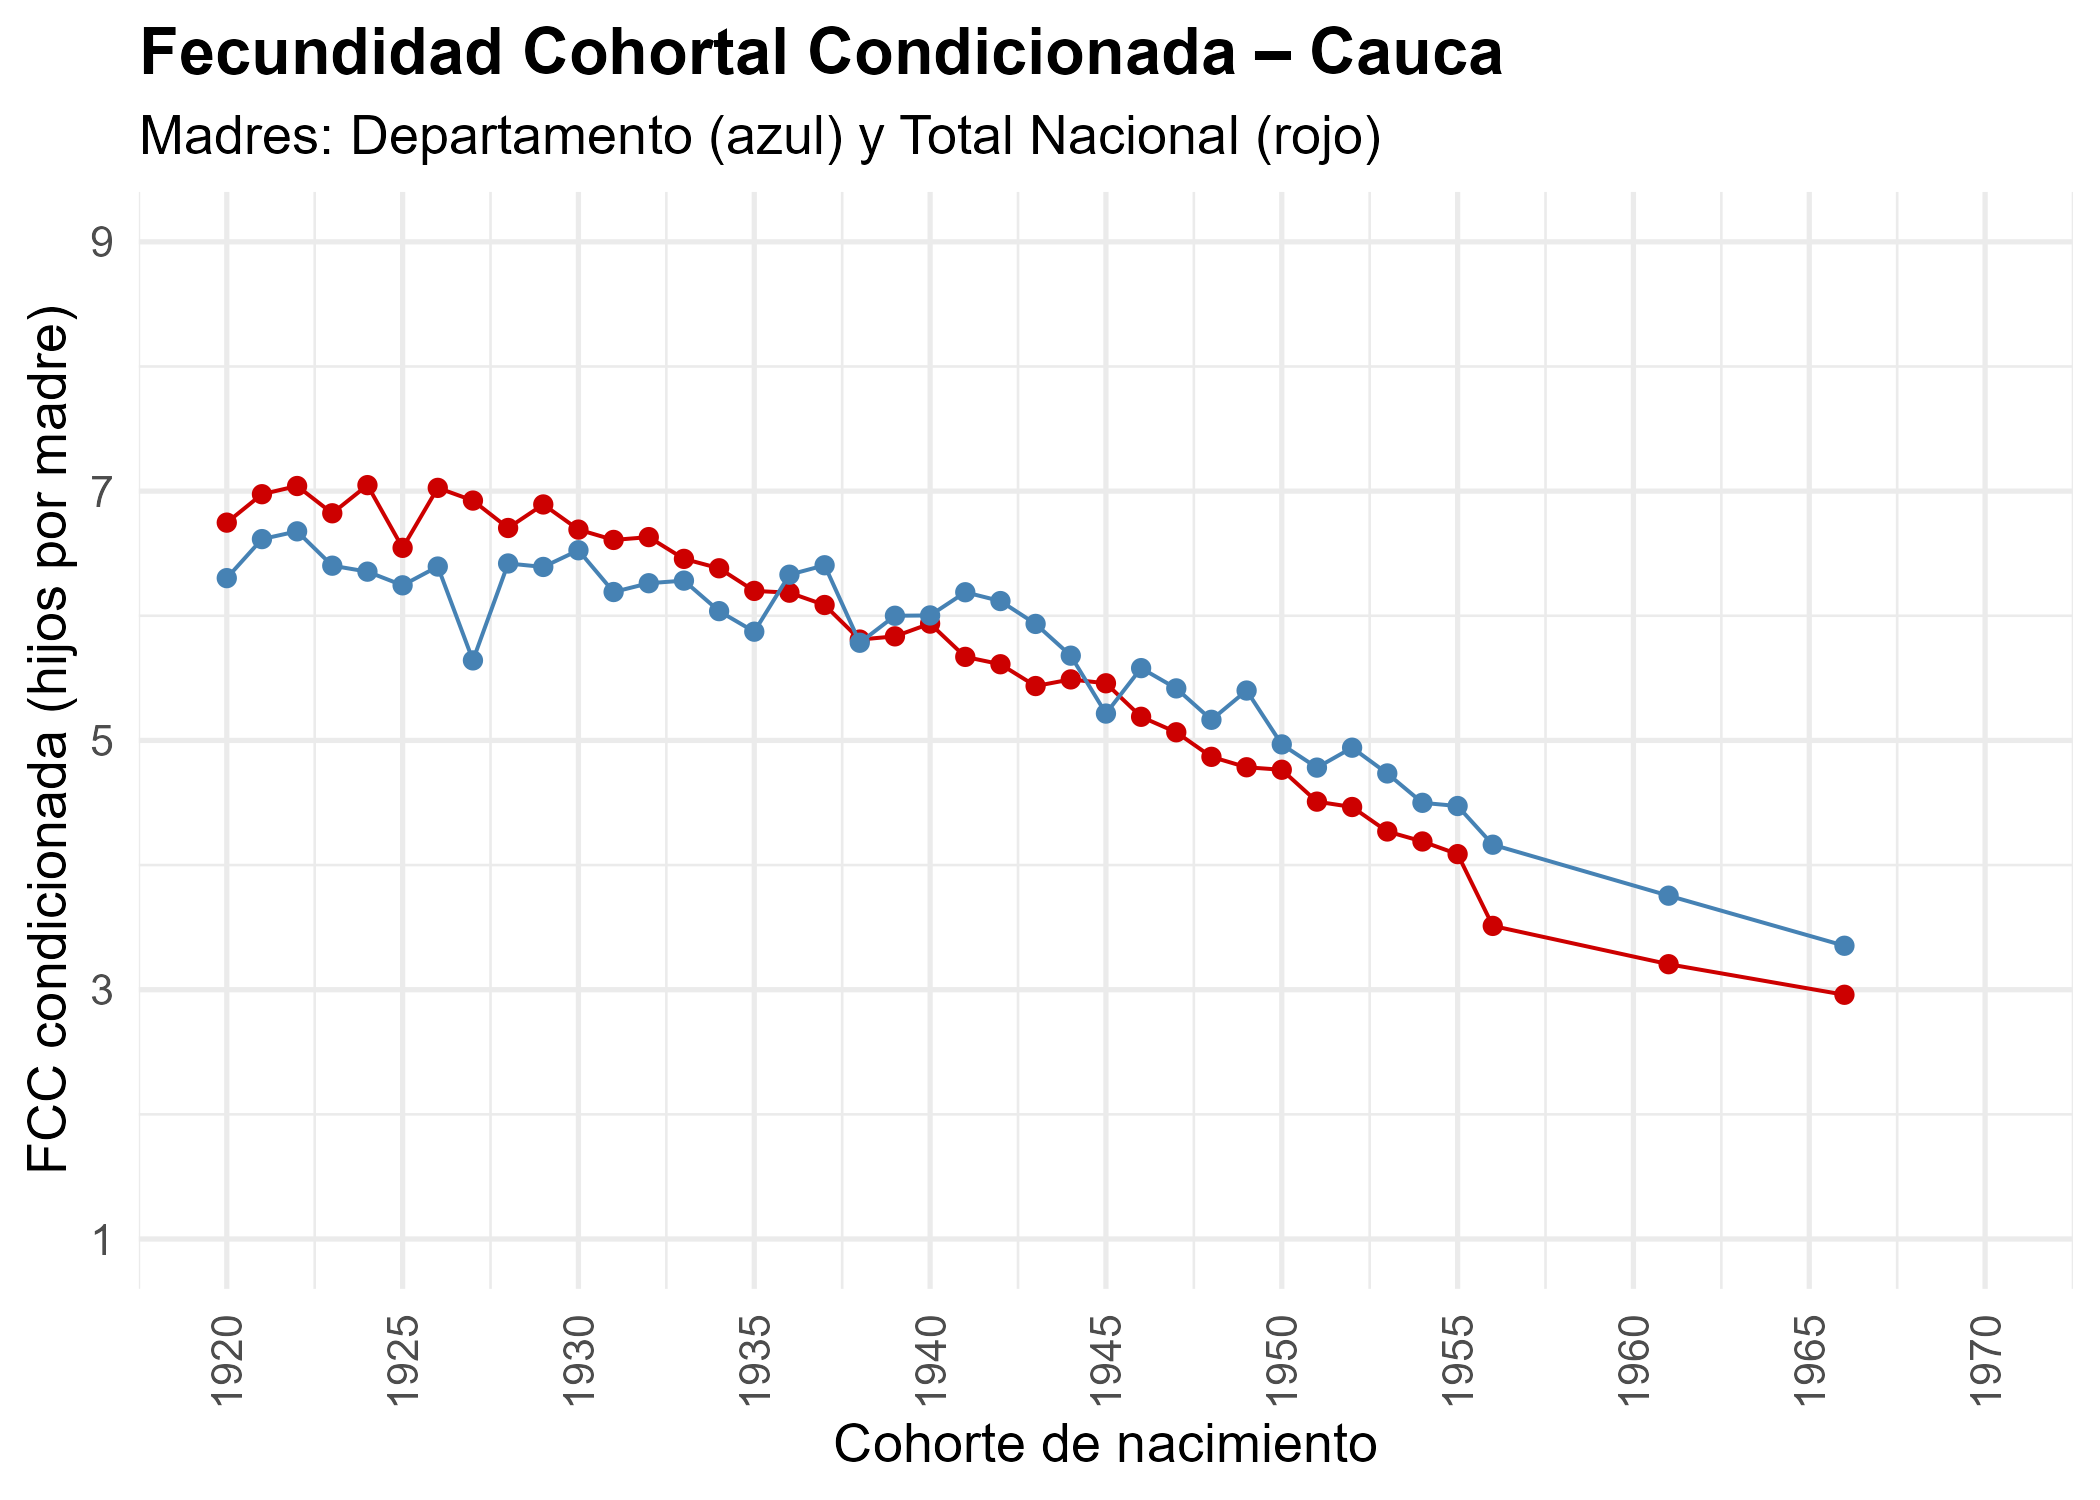
\includegraphics[width=\textwidth]{fcc_departamental/FCC_cond_Cauca_vs_National.png}
\end{columns}
\end{frame}
\begin{frame}{FCC: Cesar}
\begin{columns}
\column{0.5\textwidth}\centering
{\small Todas las mujeres}\\
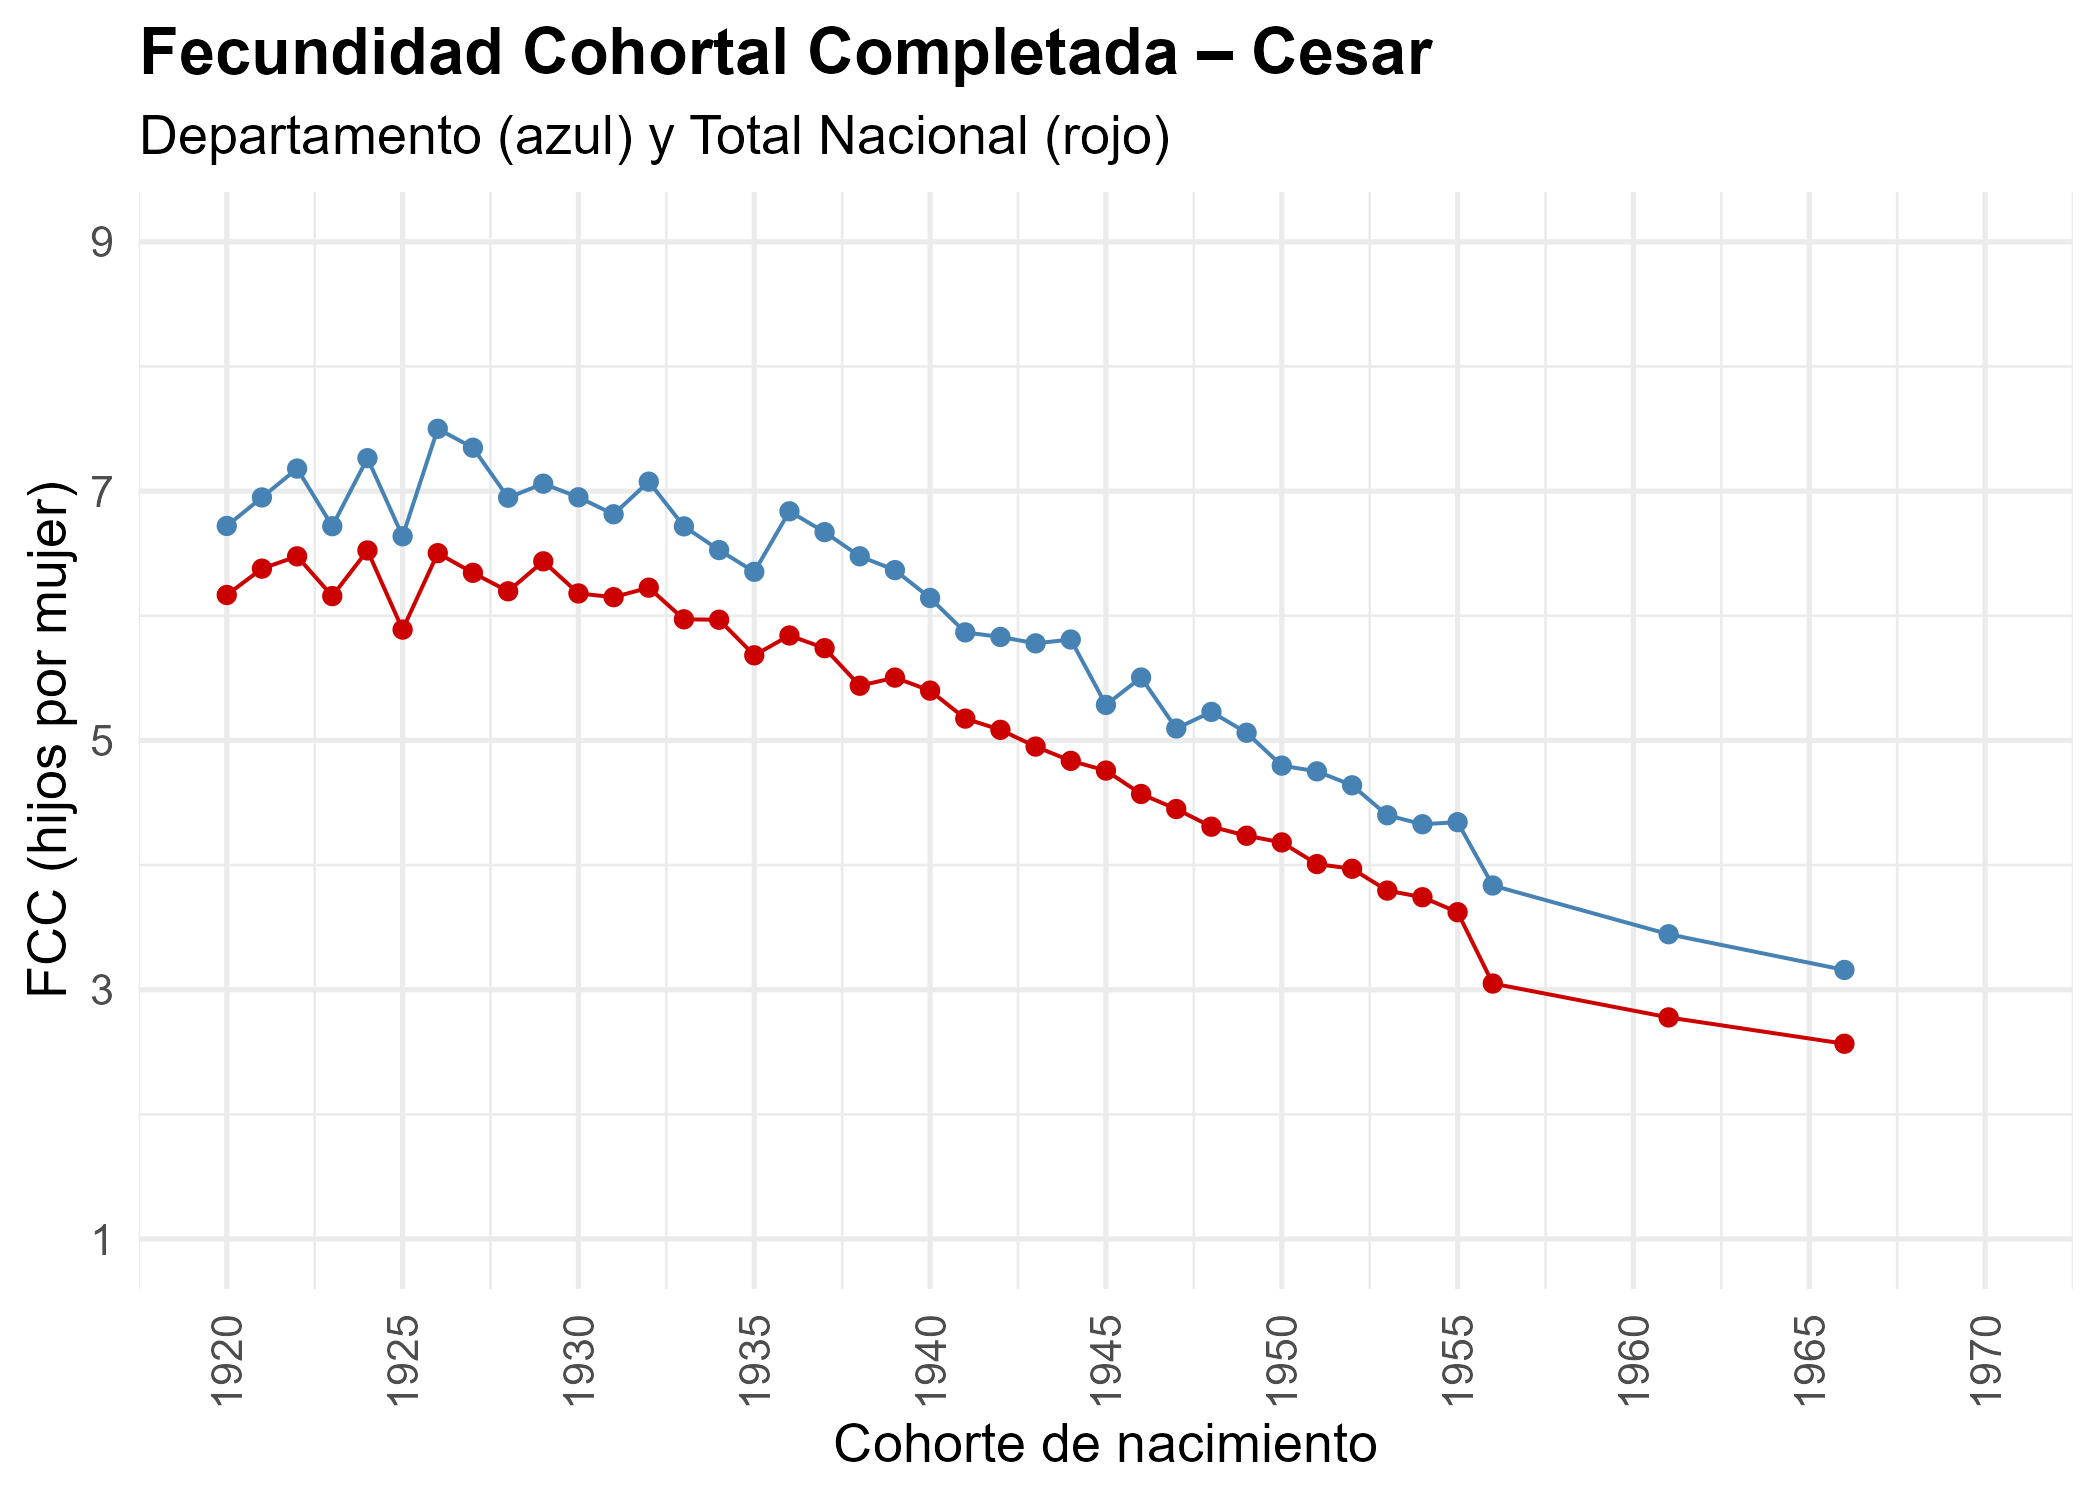
\includegraphics[width=\textwidth]{fcc_departamental/FCC_Cesar_vs_National.png}
\column{0.5\textwidth}\centering
{\small Condicional (madres)}\\
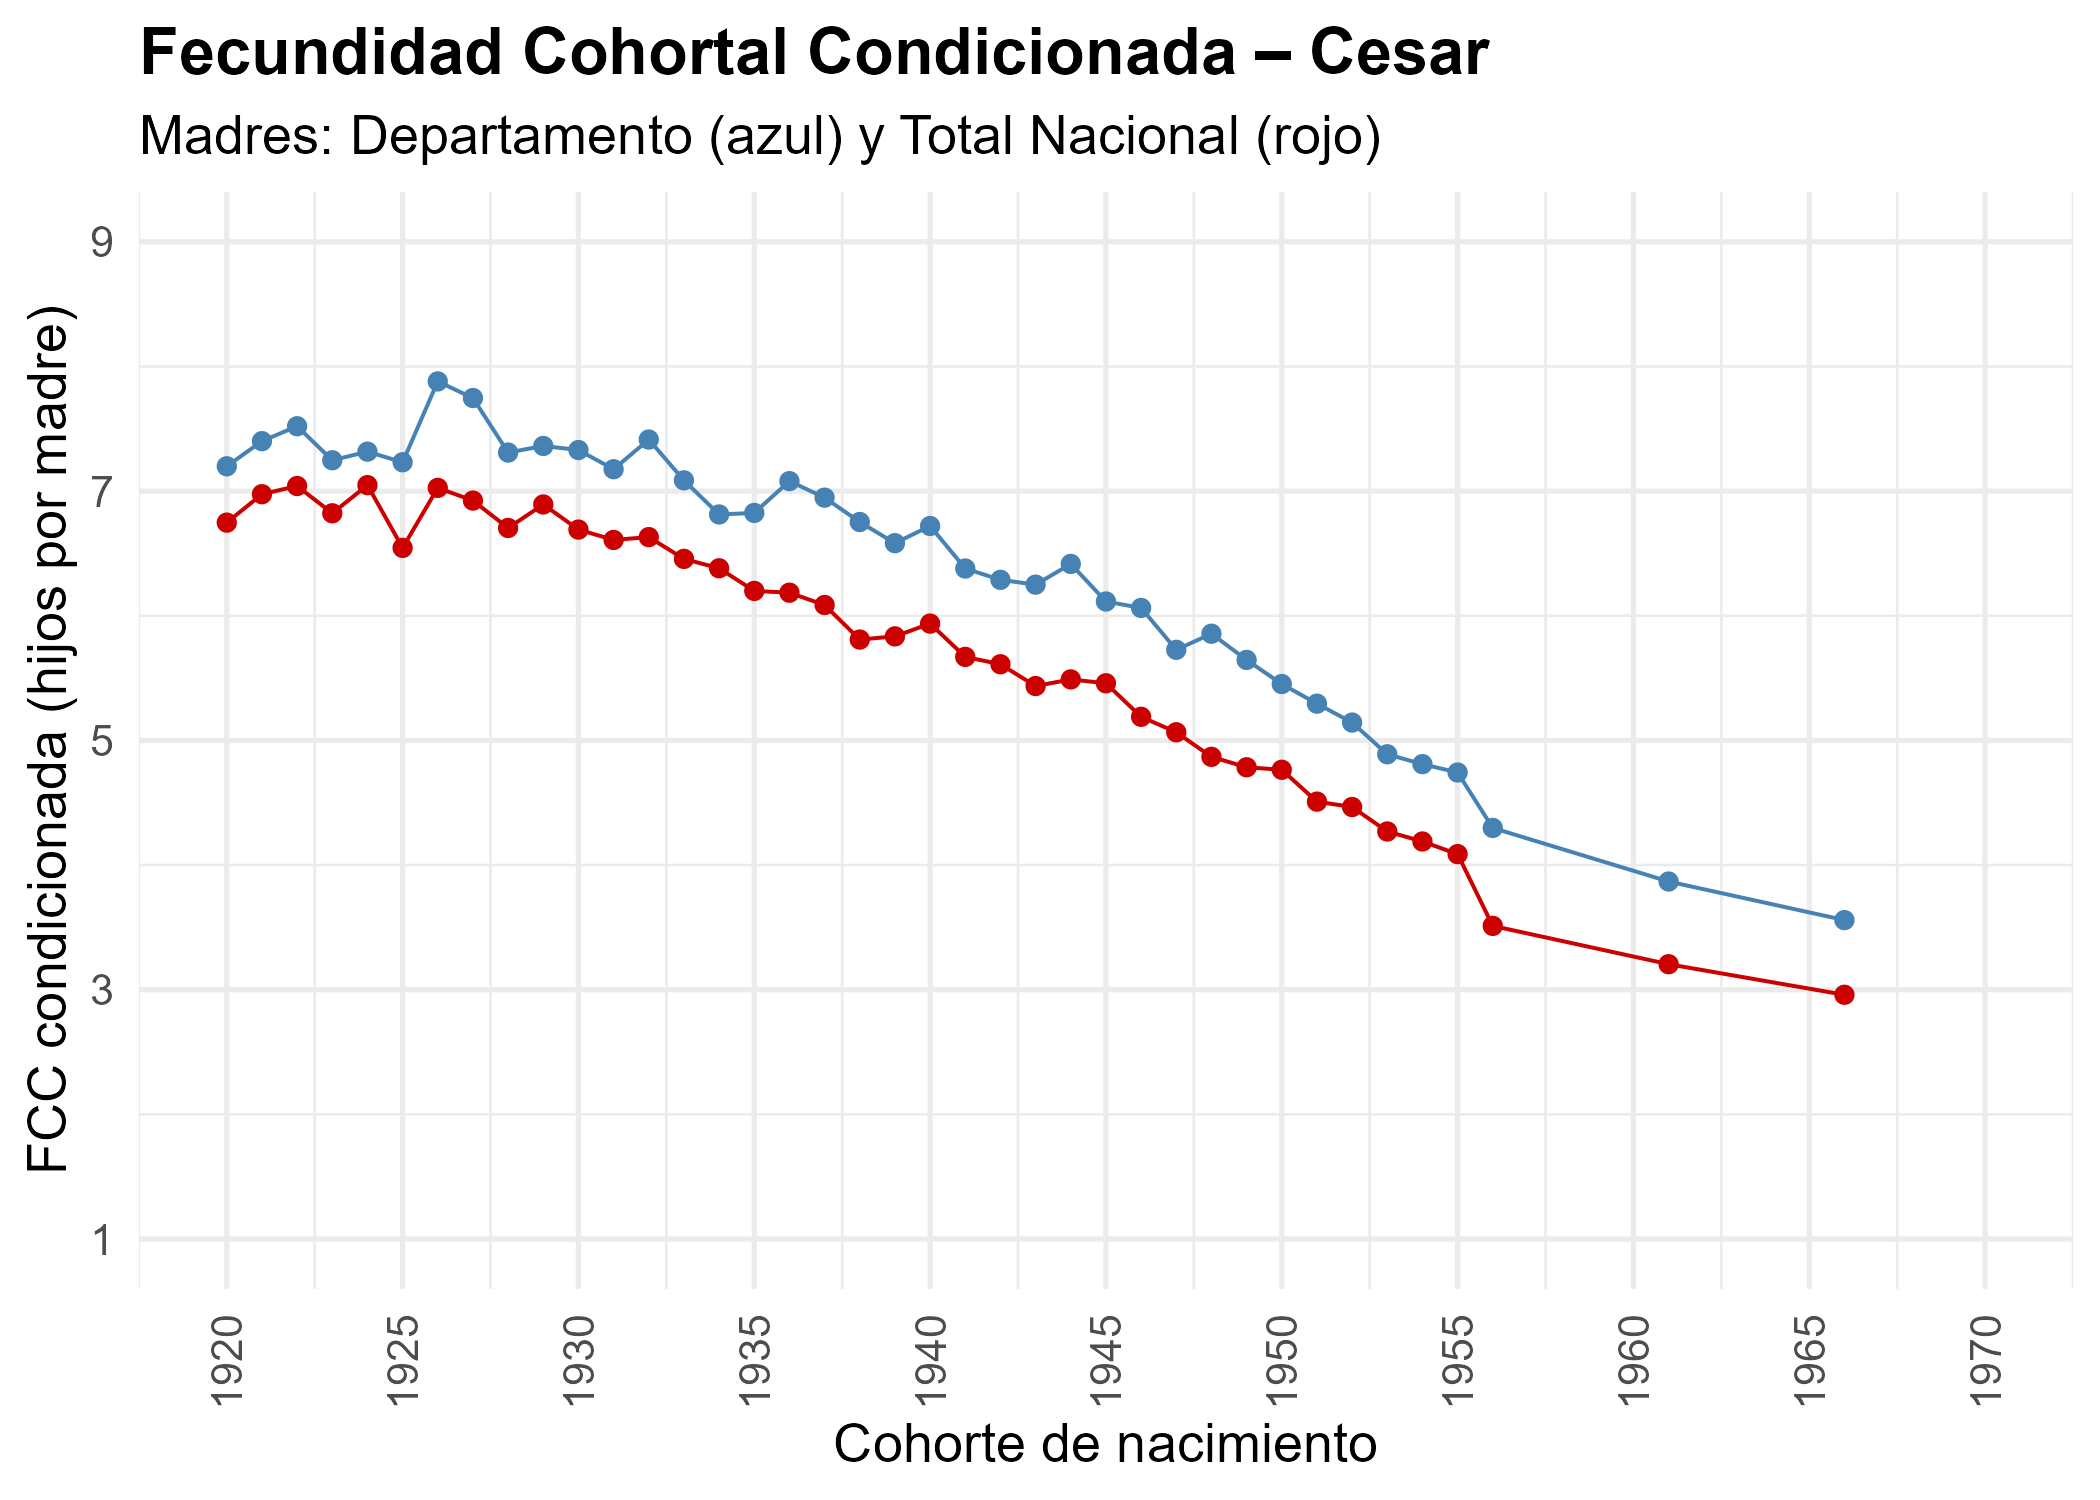
\includegraphics[width=\textwidth]{fcc_departamental/FCC_cond_Cesar_vs_National.png}
\end{columns}
\end{frame}
\begin{frame}{FCC: Chocó}
\begin{columns}
\column{0.5\textwidth}\centering
{\small Todas las mujeres}\\
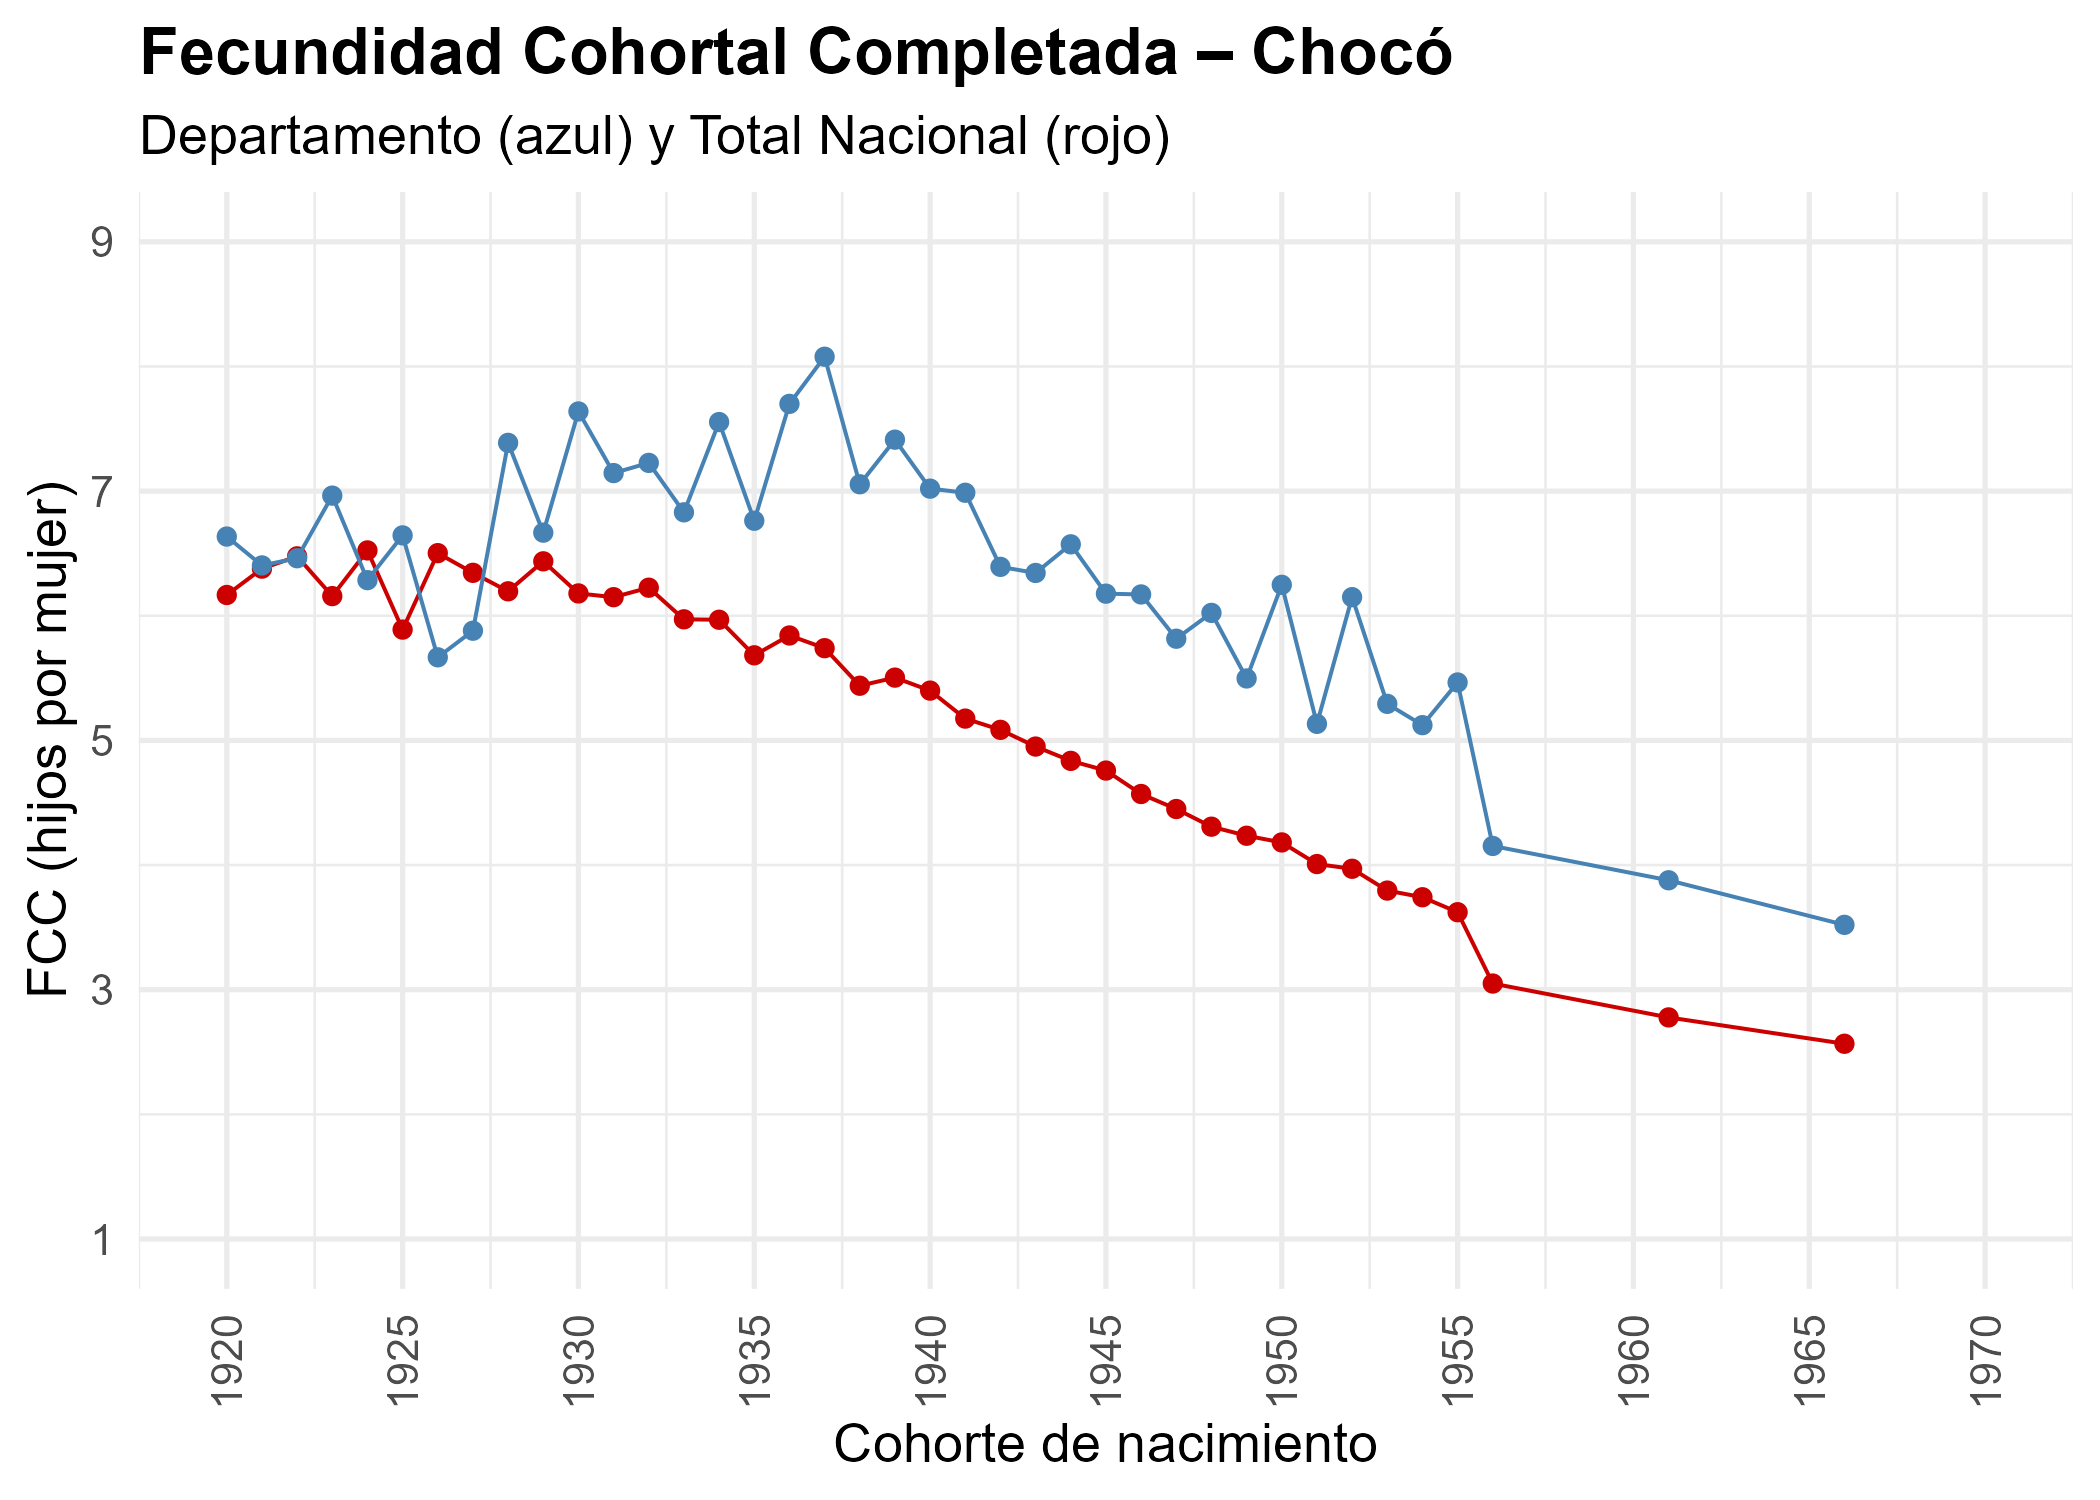
\includegraphics[width=\textwidth]{fcc_departamental/FCC_Chocó_vs_National.png}
\column{0.5\textwidth}\centering
{\small Condicional (madres)}\\
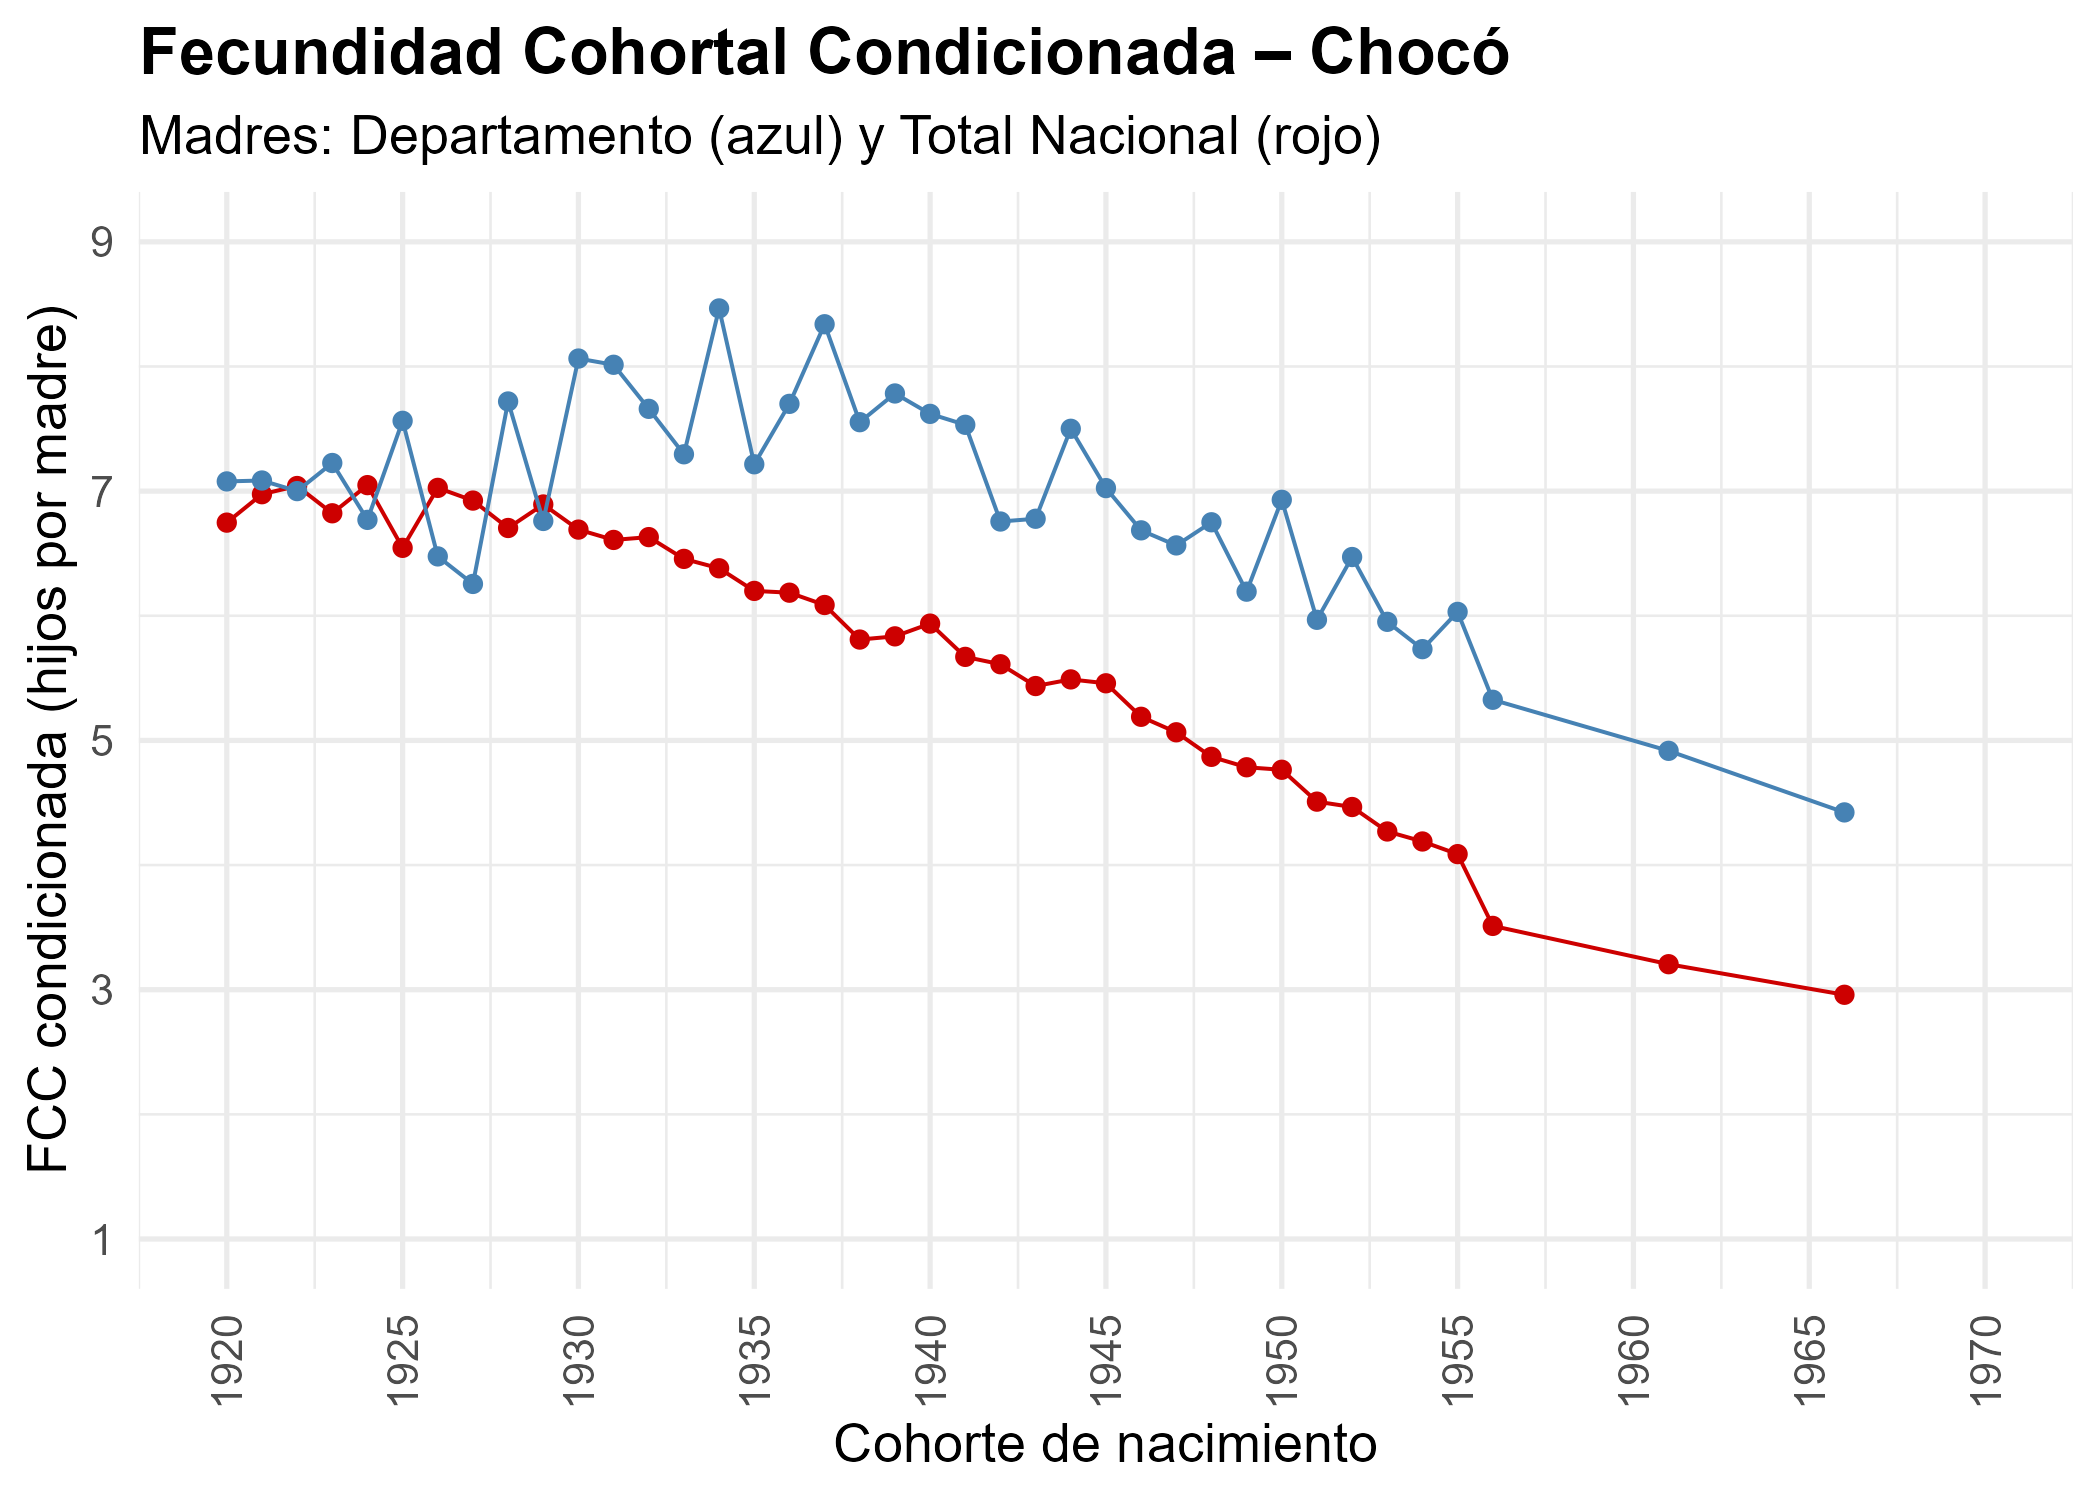
\includegraphics[width=\textwidth]{fcc_departamental/FCC_cond_Chocó_vs_National.png}
\end{columns}
\end{frame}
\begin{frame}{FCC: Córdoba}
\begin{columns}
\column{0.5\textwidth}\centering
{\small Todas las mujeres}\\
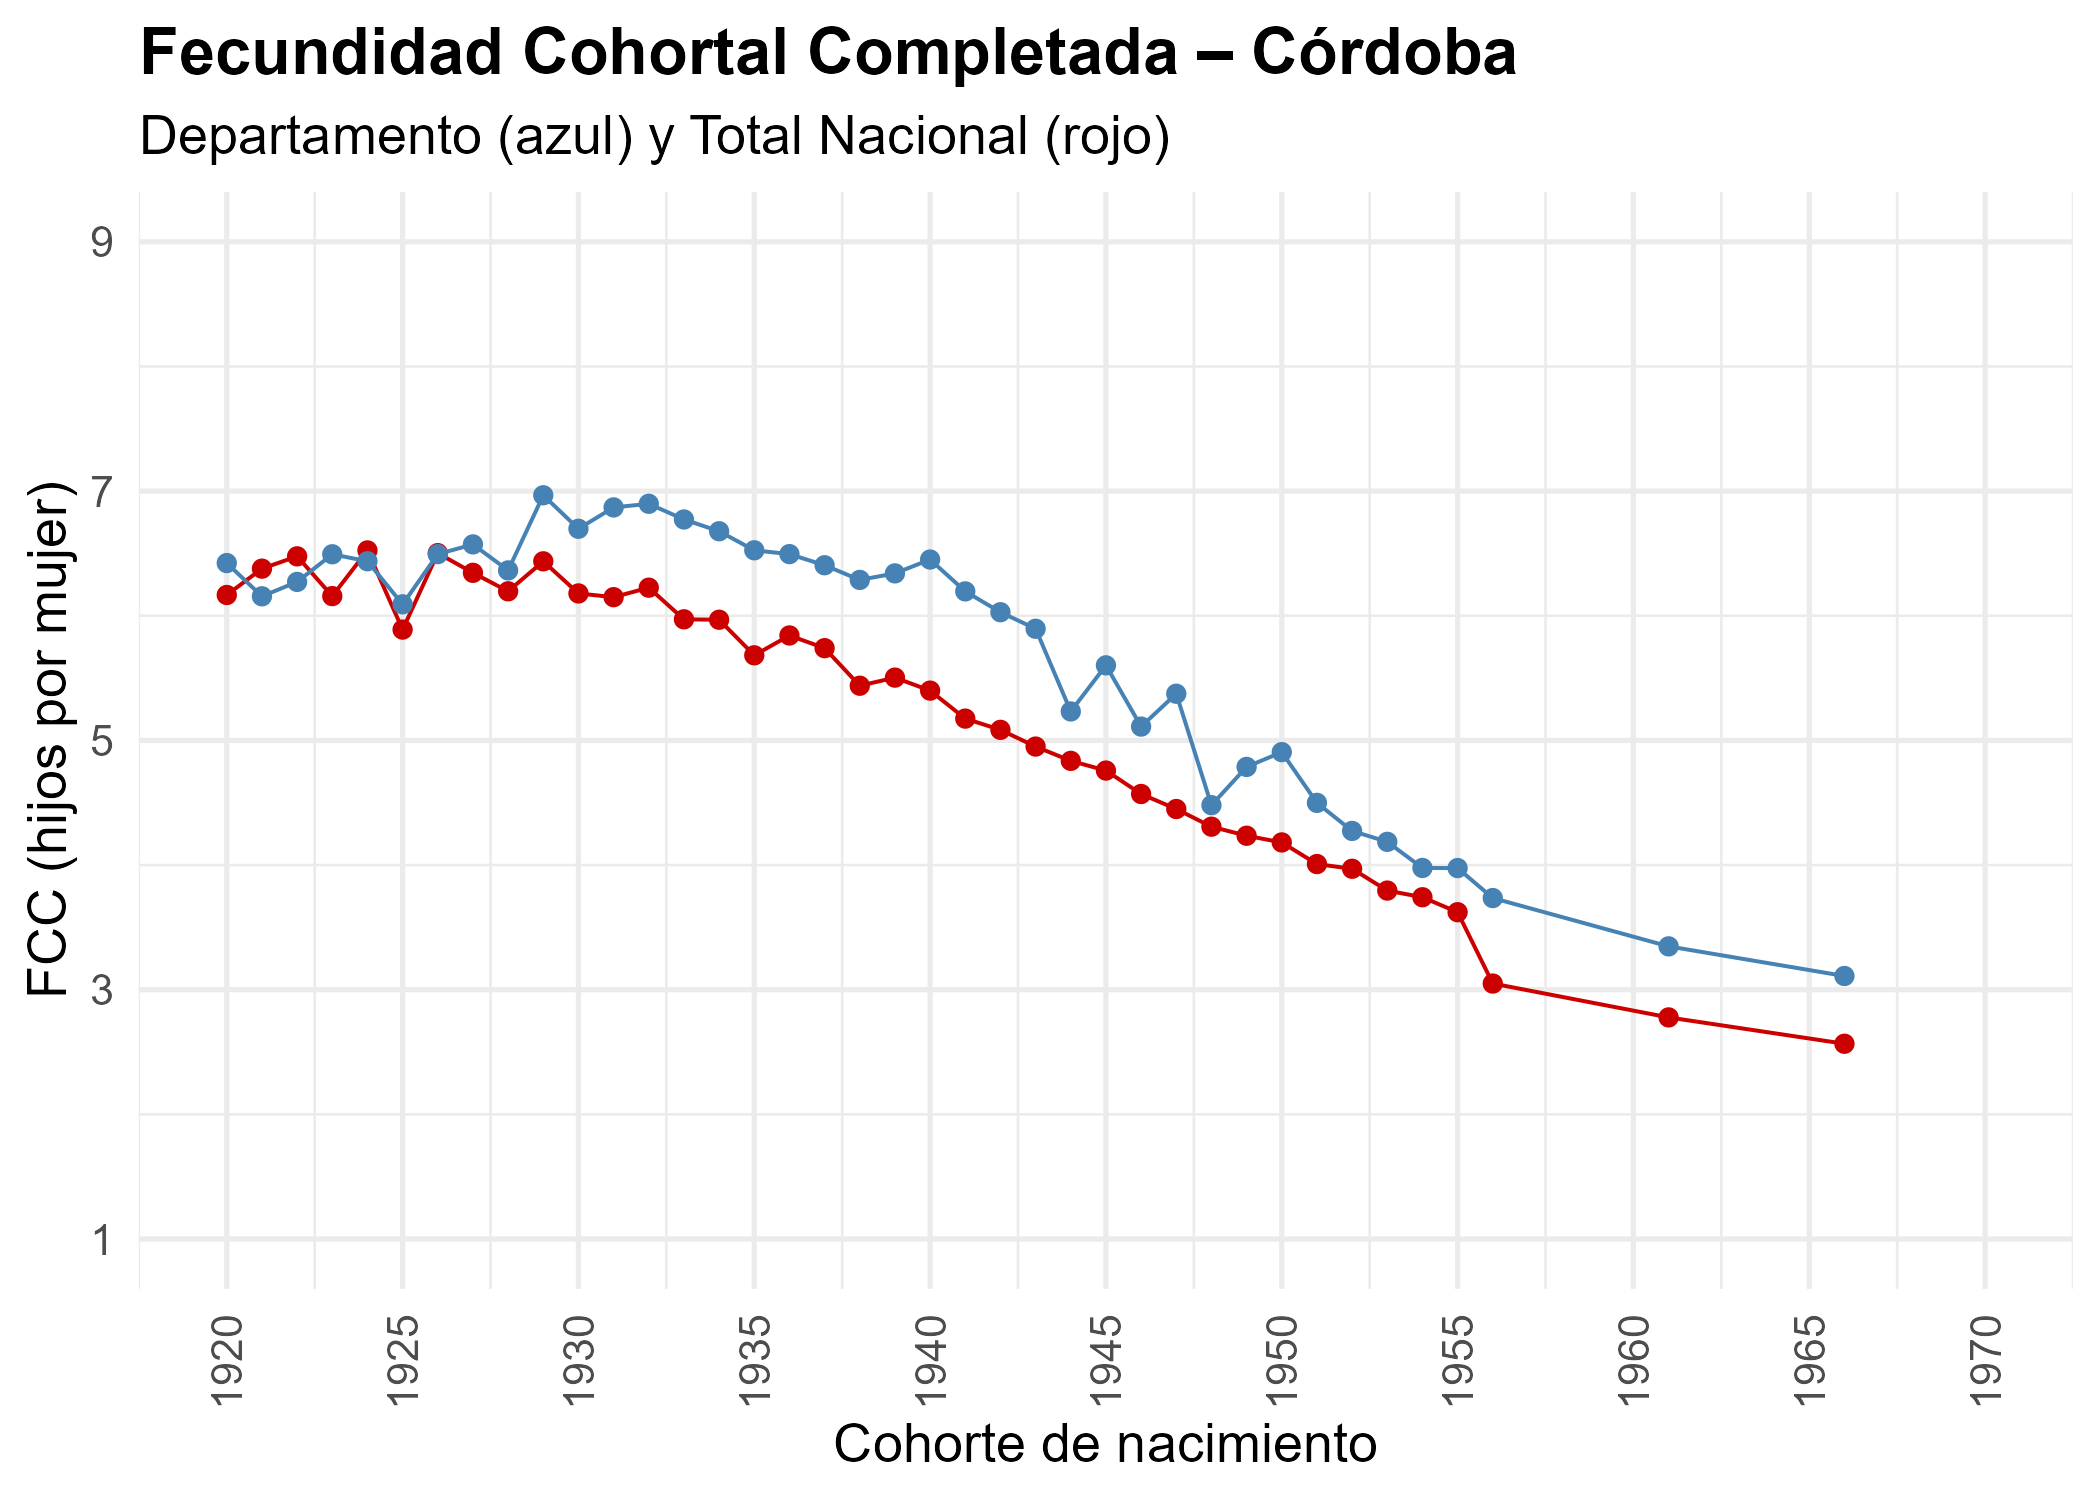
\includegraphics[width=\textwidth]{fcc_departamental/FCC_Córdoba_vs_National.png}
\column{0.5\textwidth}\centering
{\small Condicional (madres)}\\
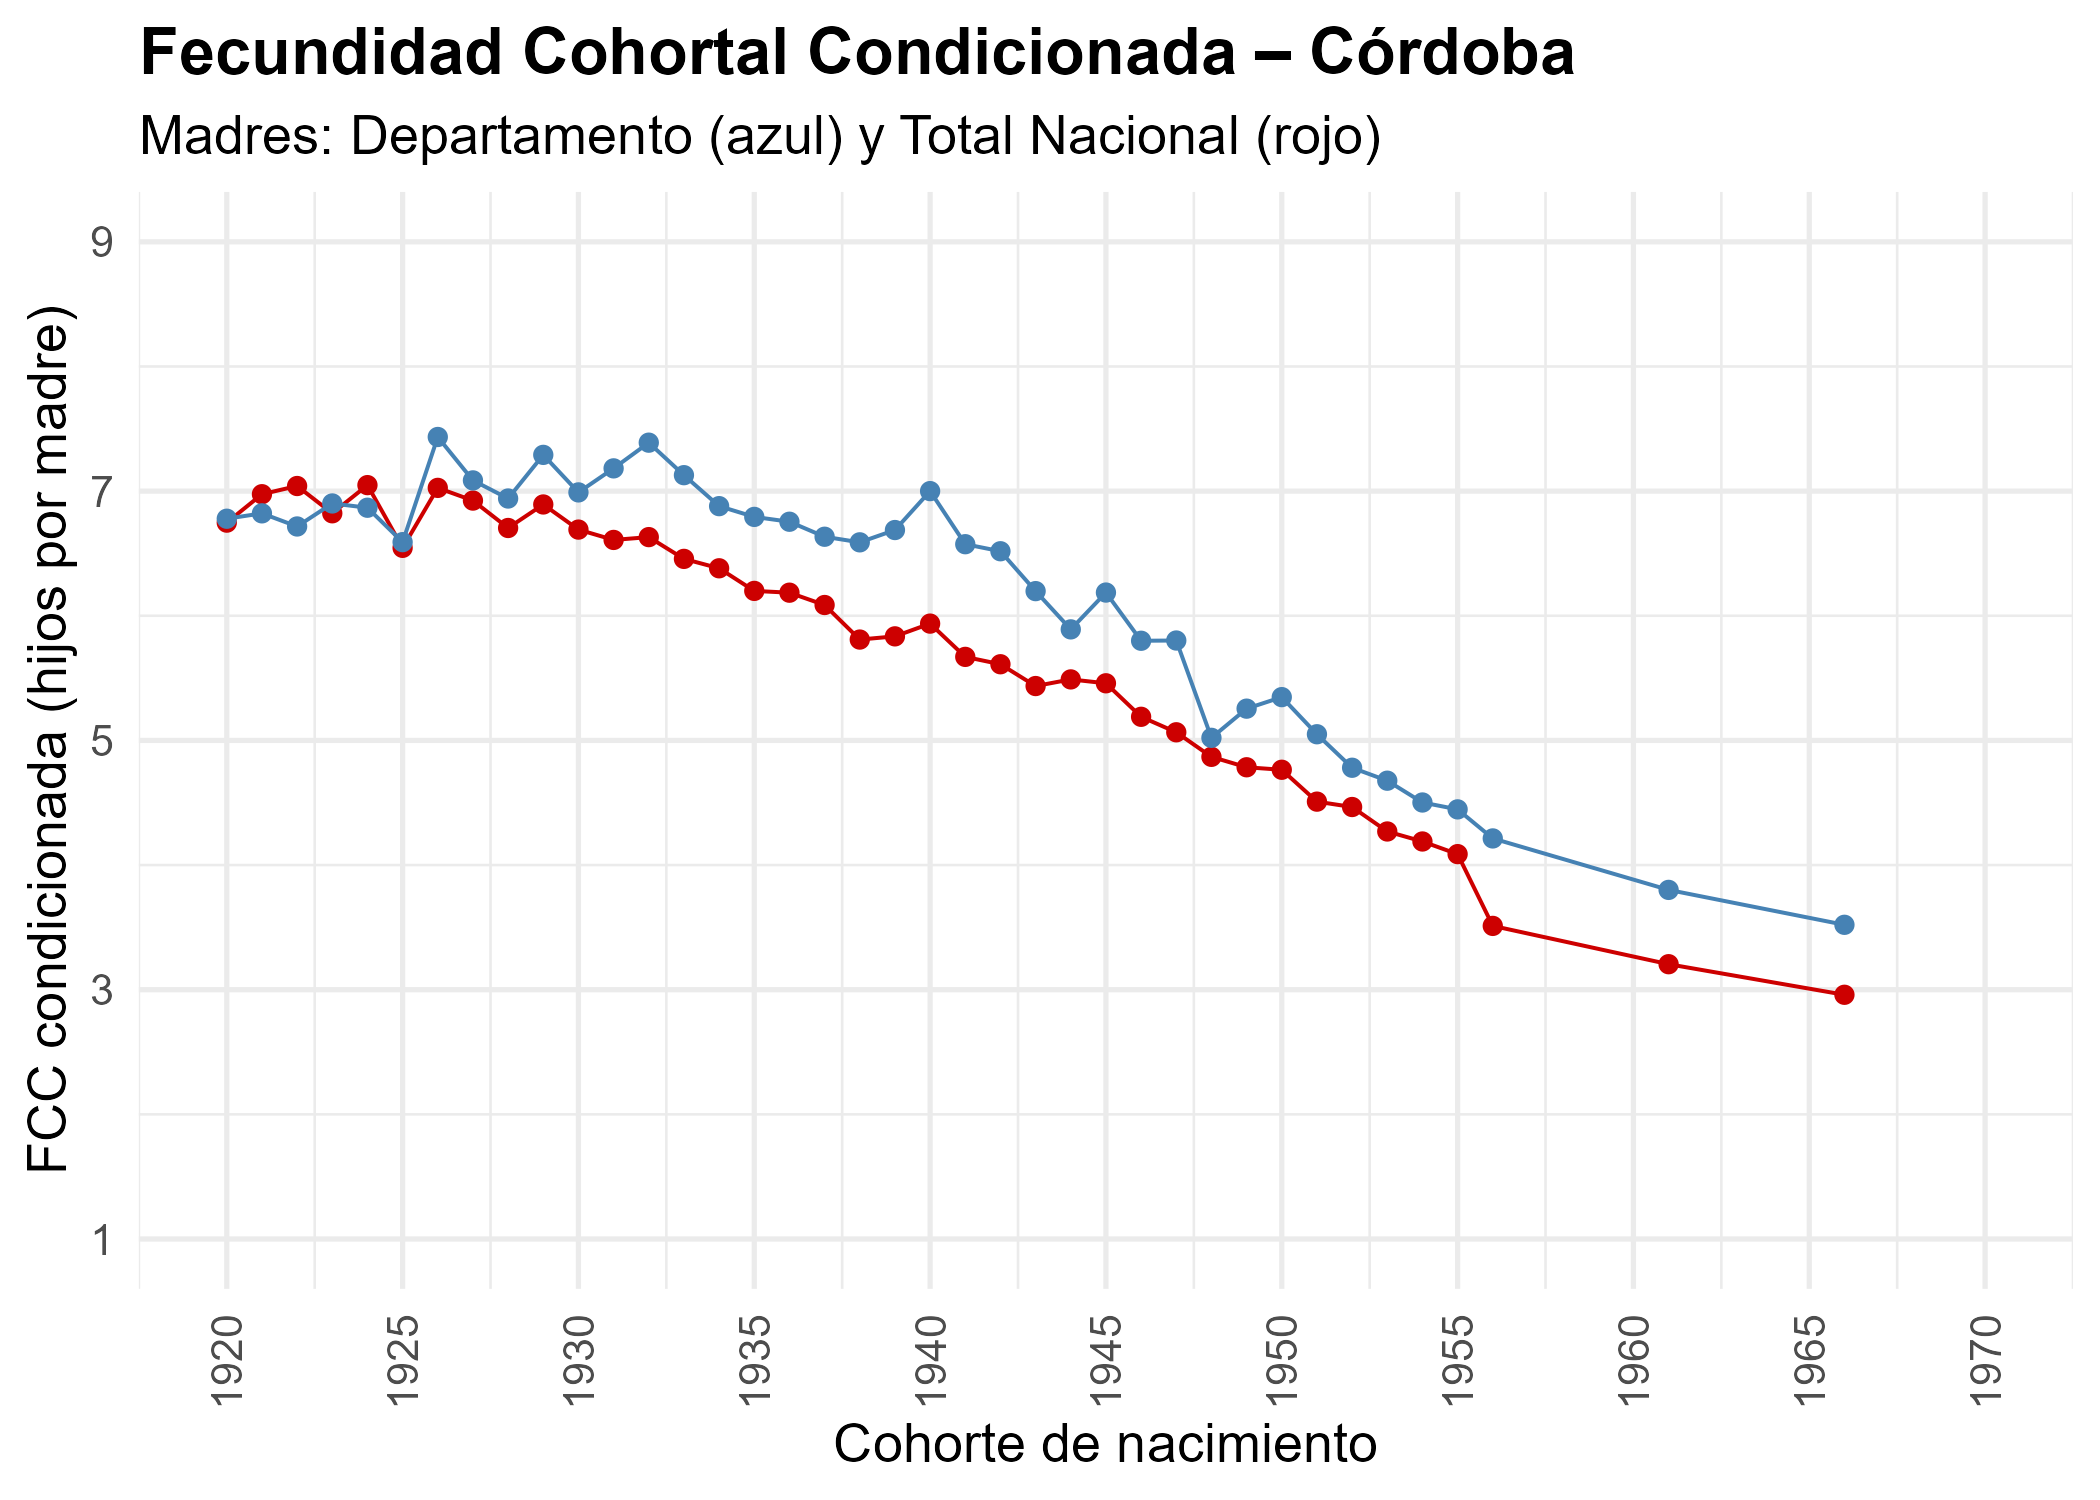
\includegraphics[width=\textwidth]{fcc_departamental/FCC_cond_Córdoba_vs_National.png}
\end{columns}
\end{frame}
\begin{frame}{FCC: Huila}
\begin{columns}
\column{0.5\textwidth}\centering
{\small Todas las mujeres}\\
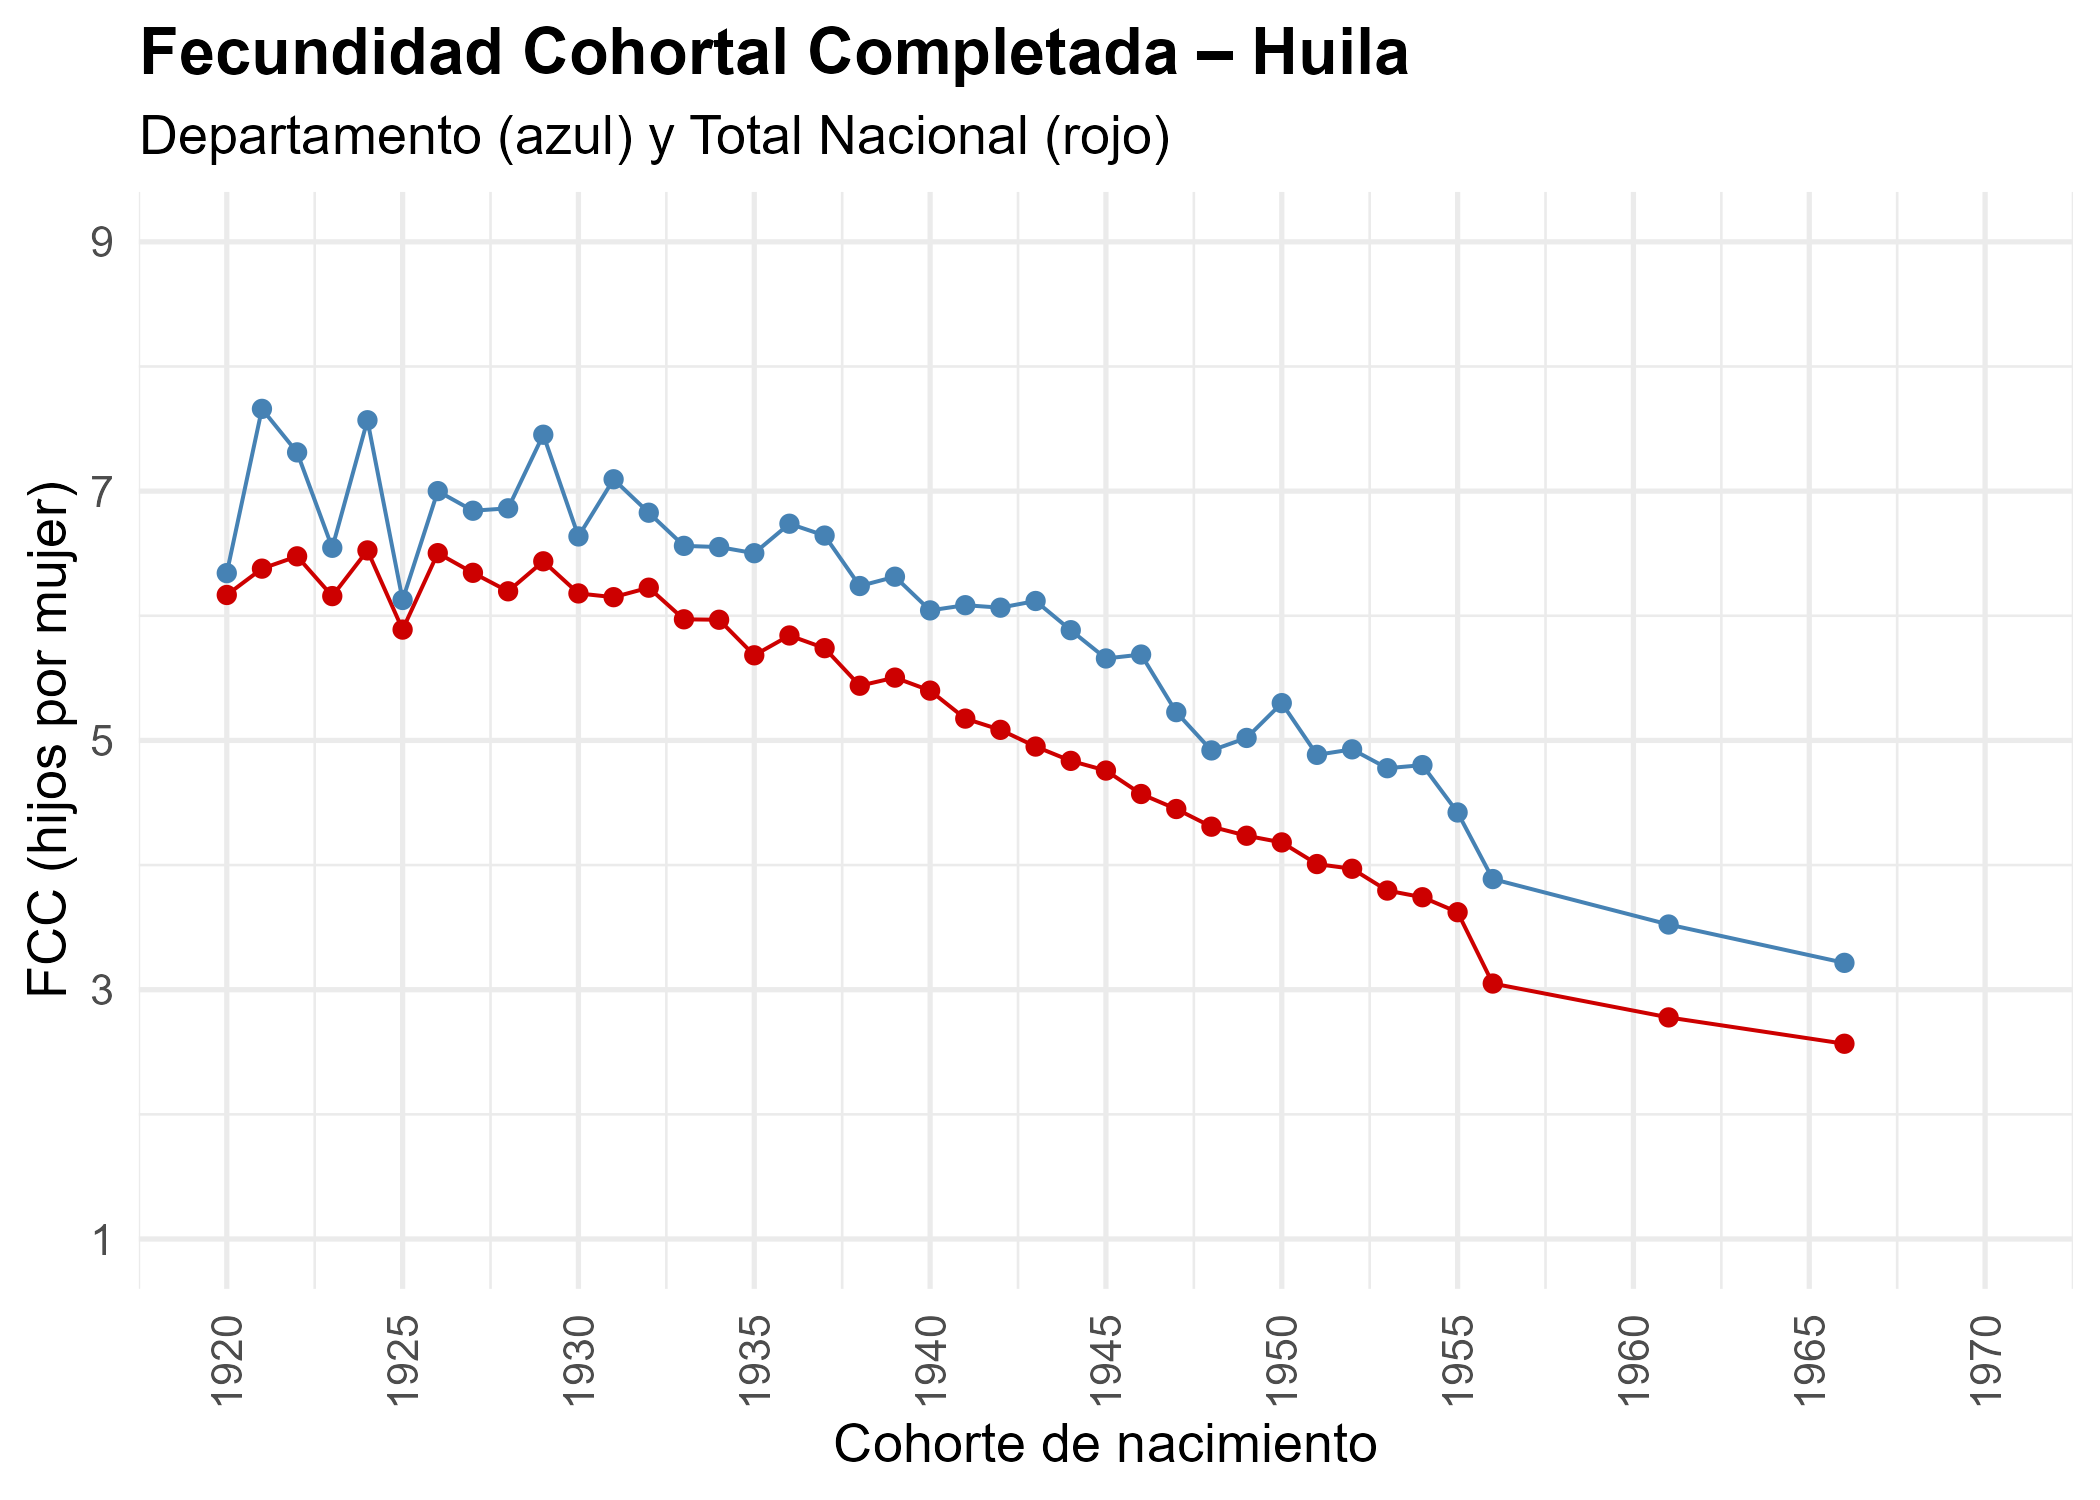
\includegraphics[width=\textwidth]{fcc_departamental/FCC_Huila_vs_National.png}
\column{0.5\textwidth}\centering
{\small Condicional (madres)}\\
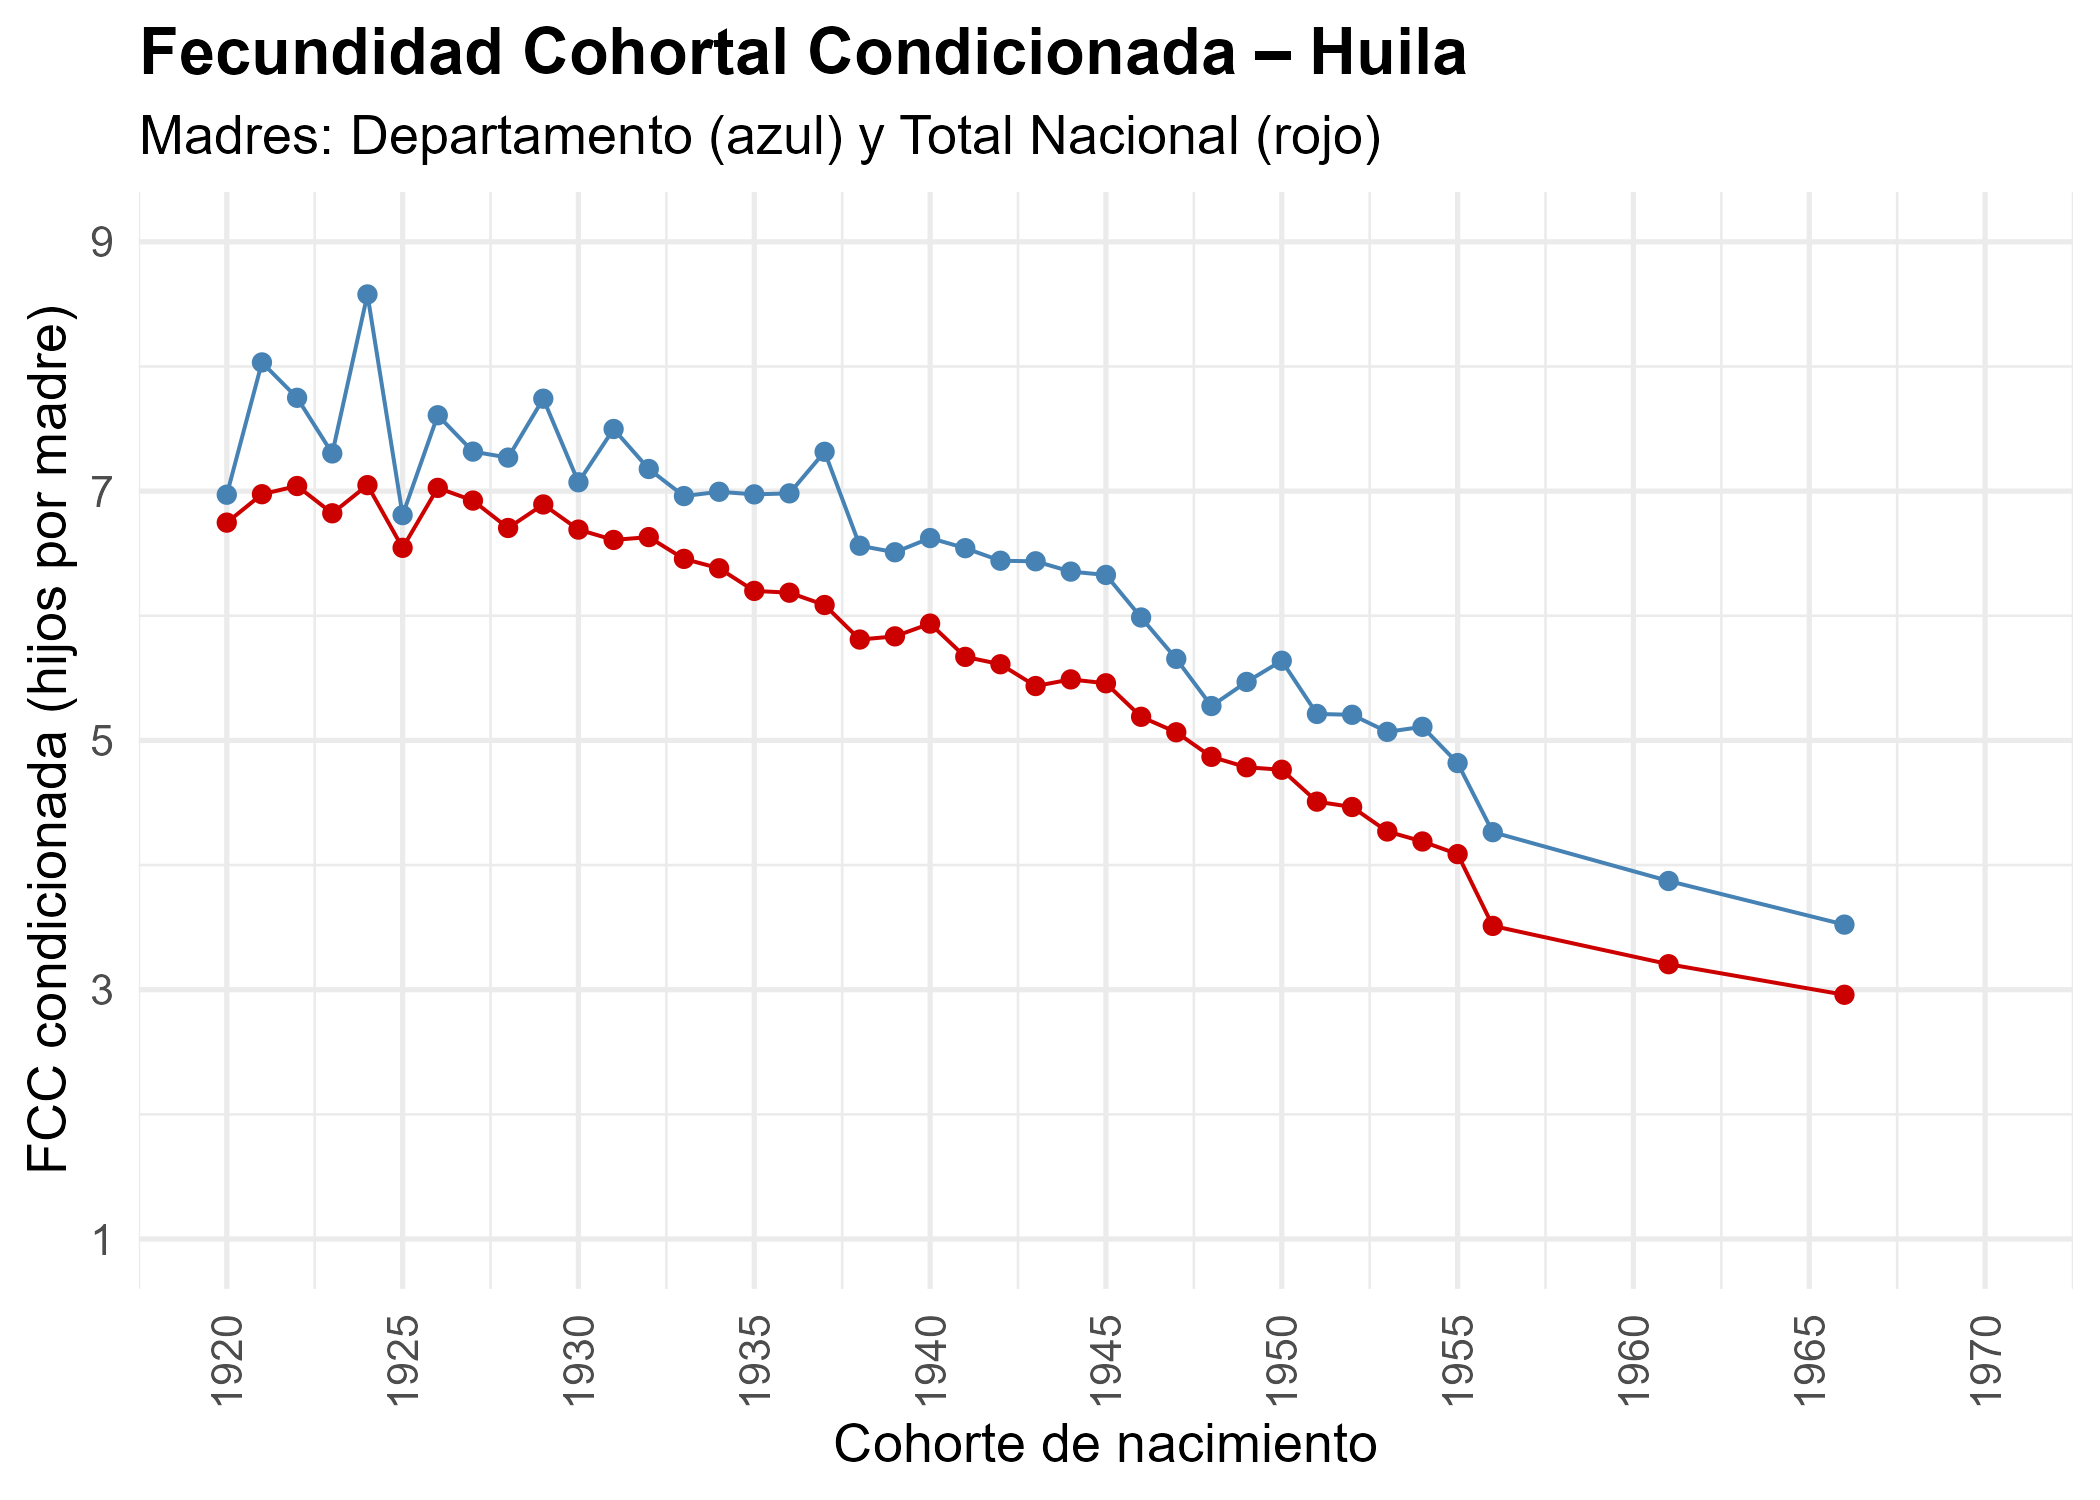
\includegraphics[width=\textwidth]{fcc_departamental/FCC_cond_Huila_vs_National.png}
\end{columns}
\end{frame}
\begin{frame}{FCC: La Guajira}
\begin{columns}
\column{0.5\textwidth}\centering
{\small Todas las mujeres}\\
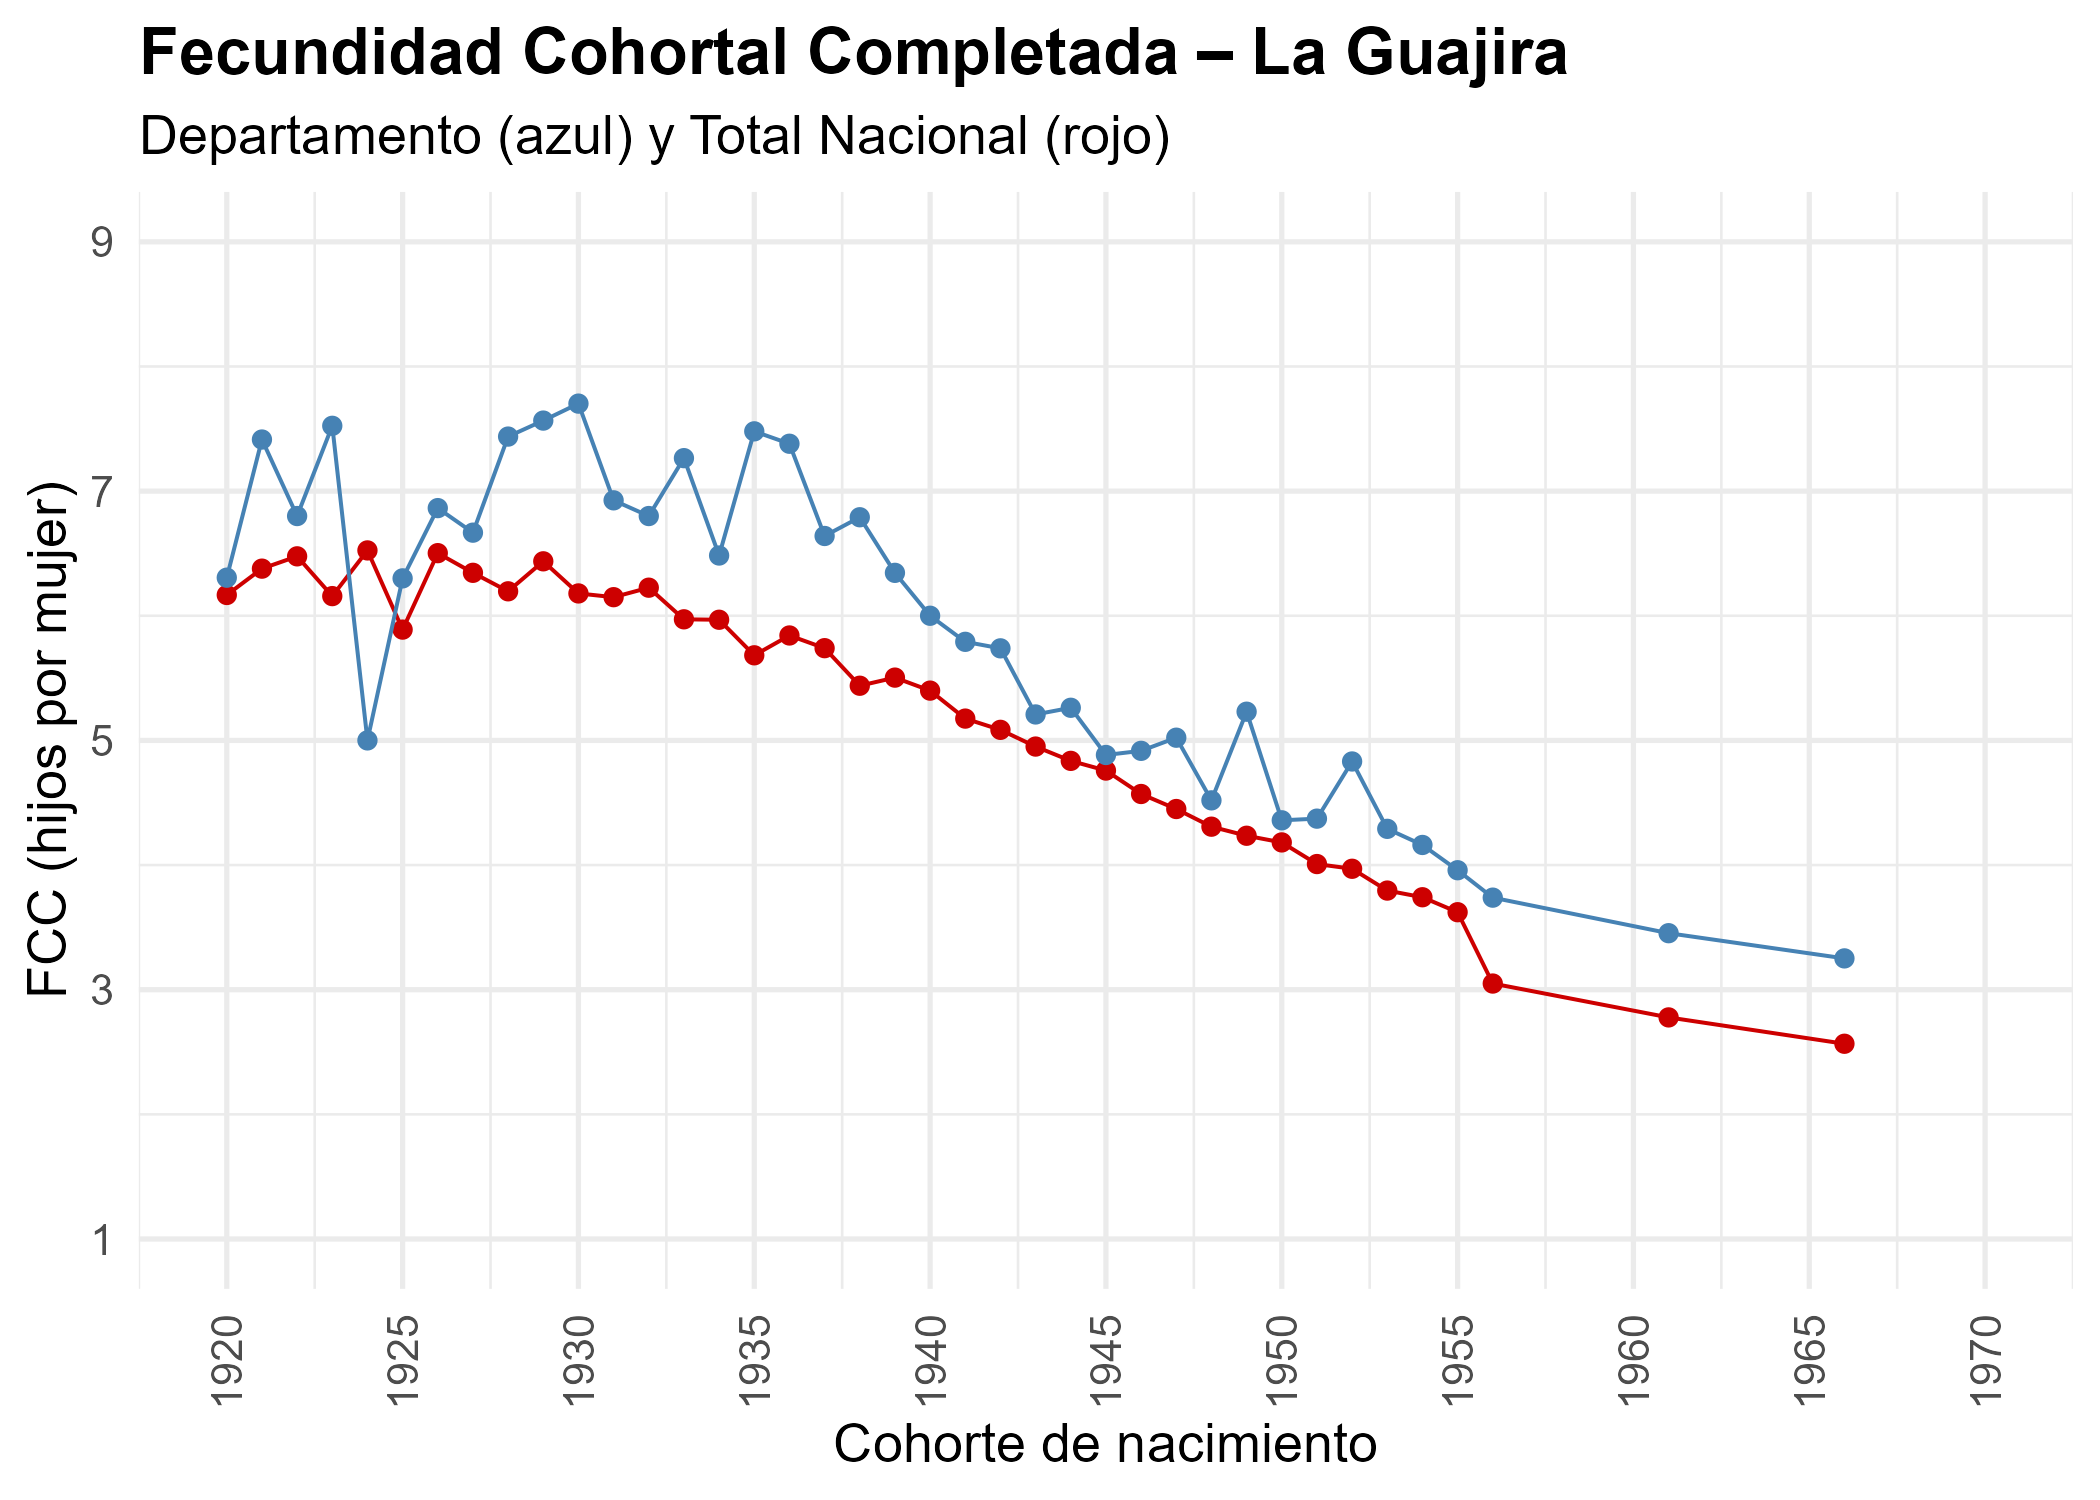
\includegraphics[width=\textwidth]{fcc_departamental/FCC_La Guajira_vs_National.png}
\column{0.5\textwidth}\centering
{\small Condicional (madres)}\\
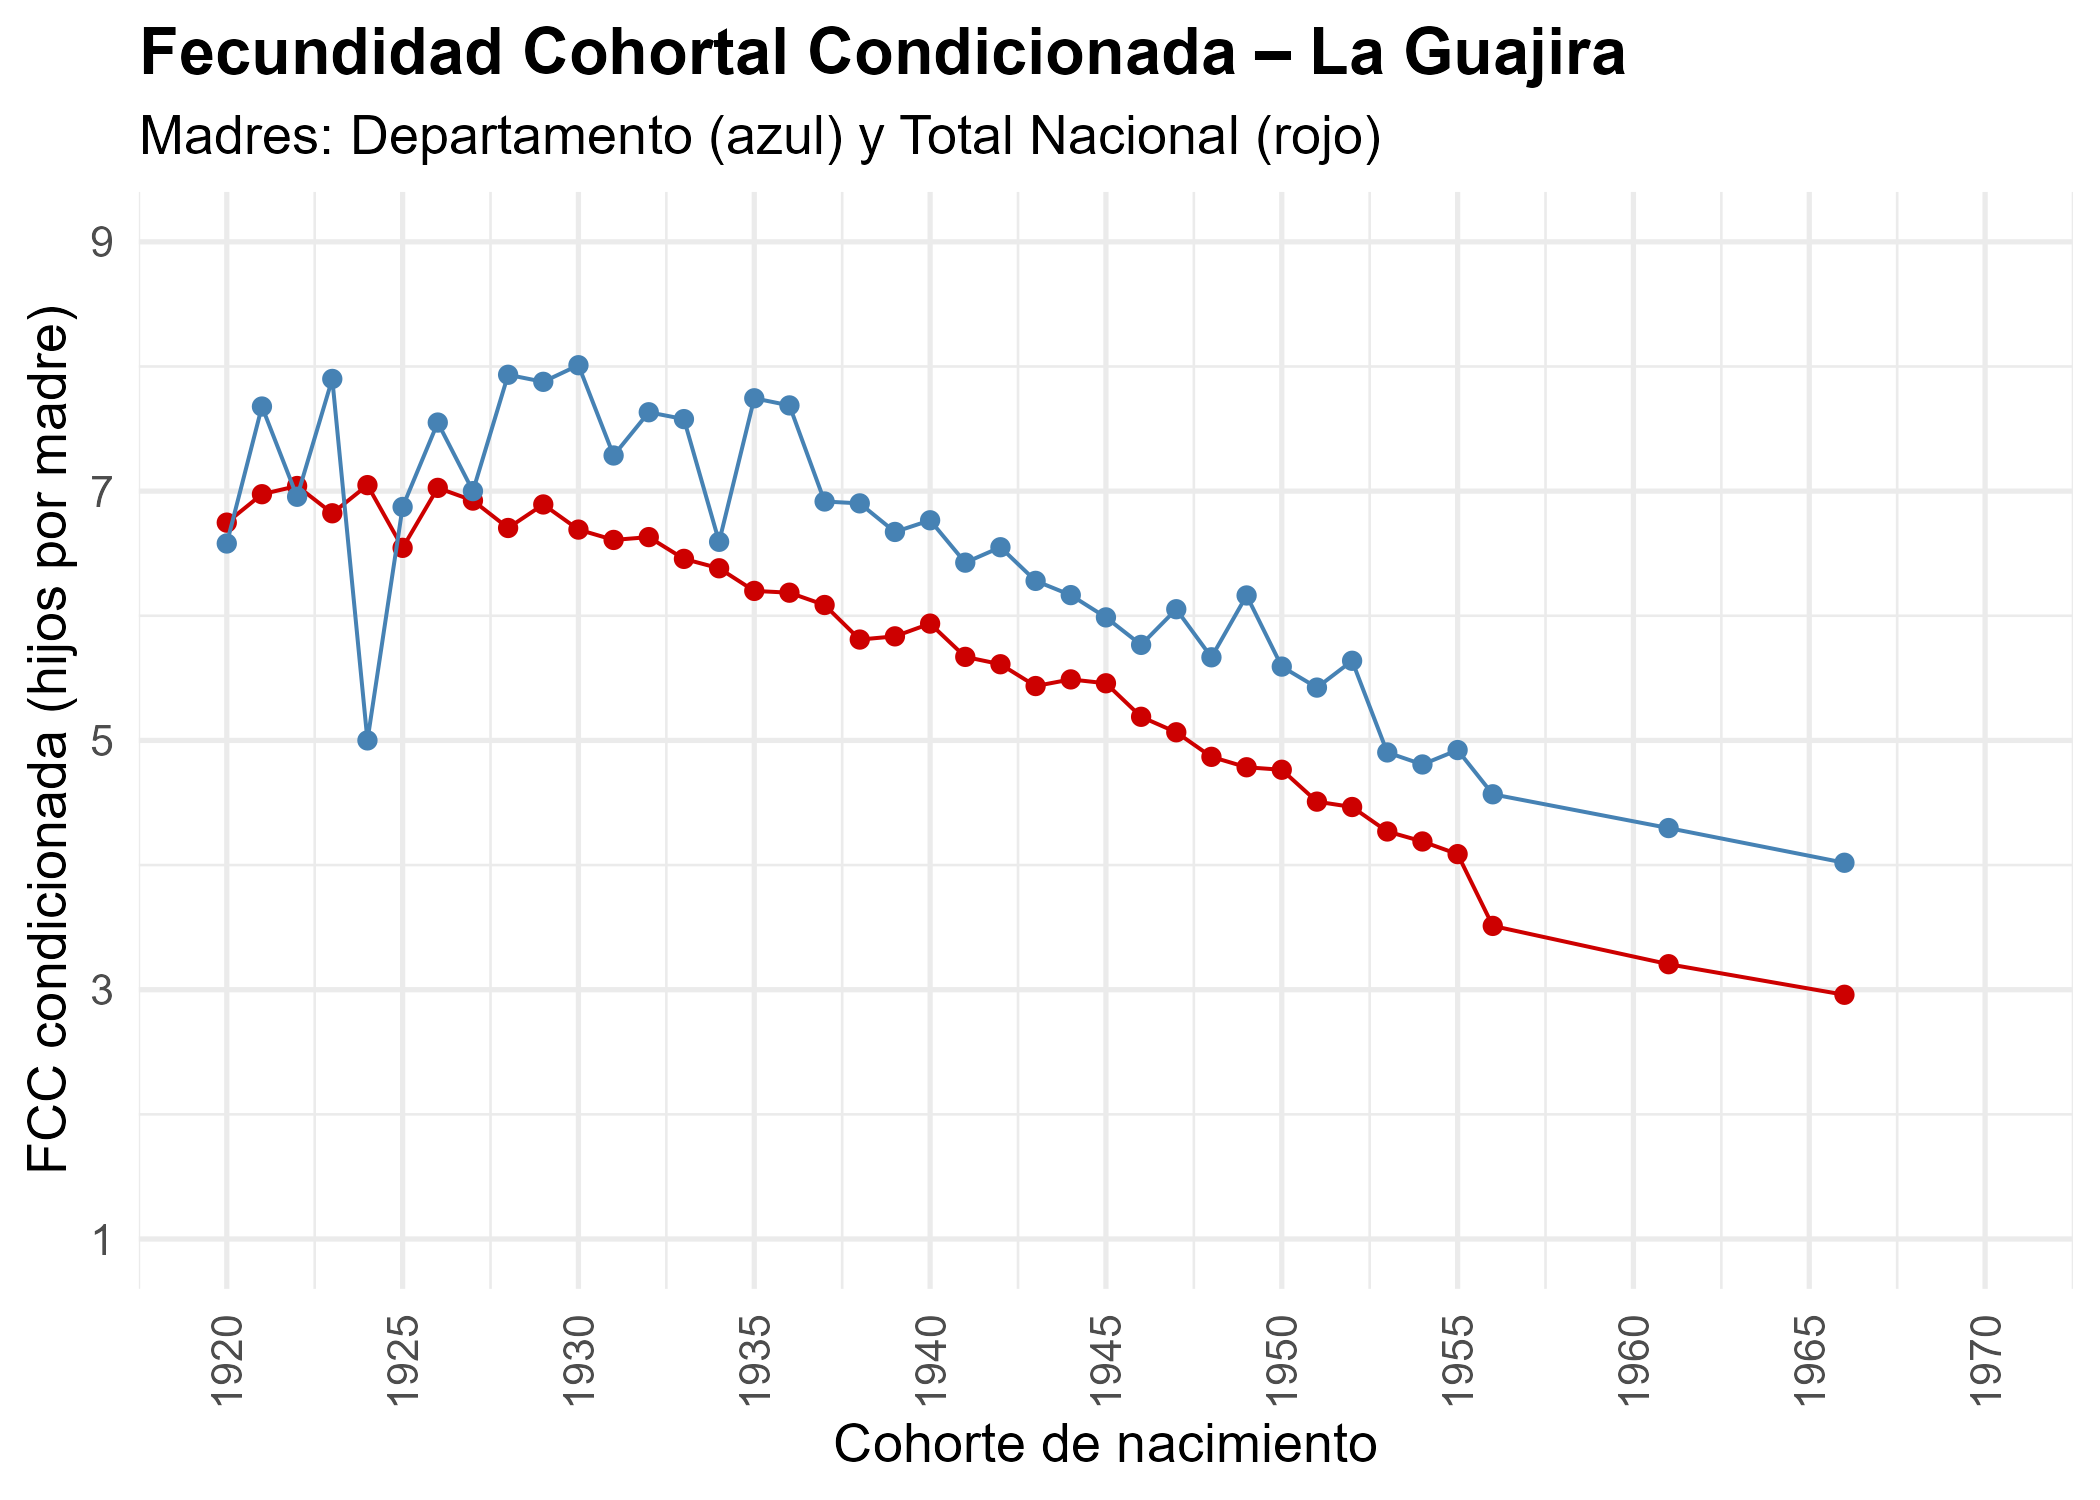
\includegraphics[width=\textwidth]{fcc_departamental/FCC_cond_La Guajira_vs_National.png}
\end{columns}
\end{frame}
\begin{frame}{FCC: Meta}
\begin{columns}
\column{0.5\textwidth}\centering
{\small Todas las mujeres}\\
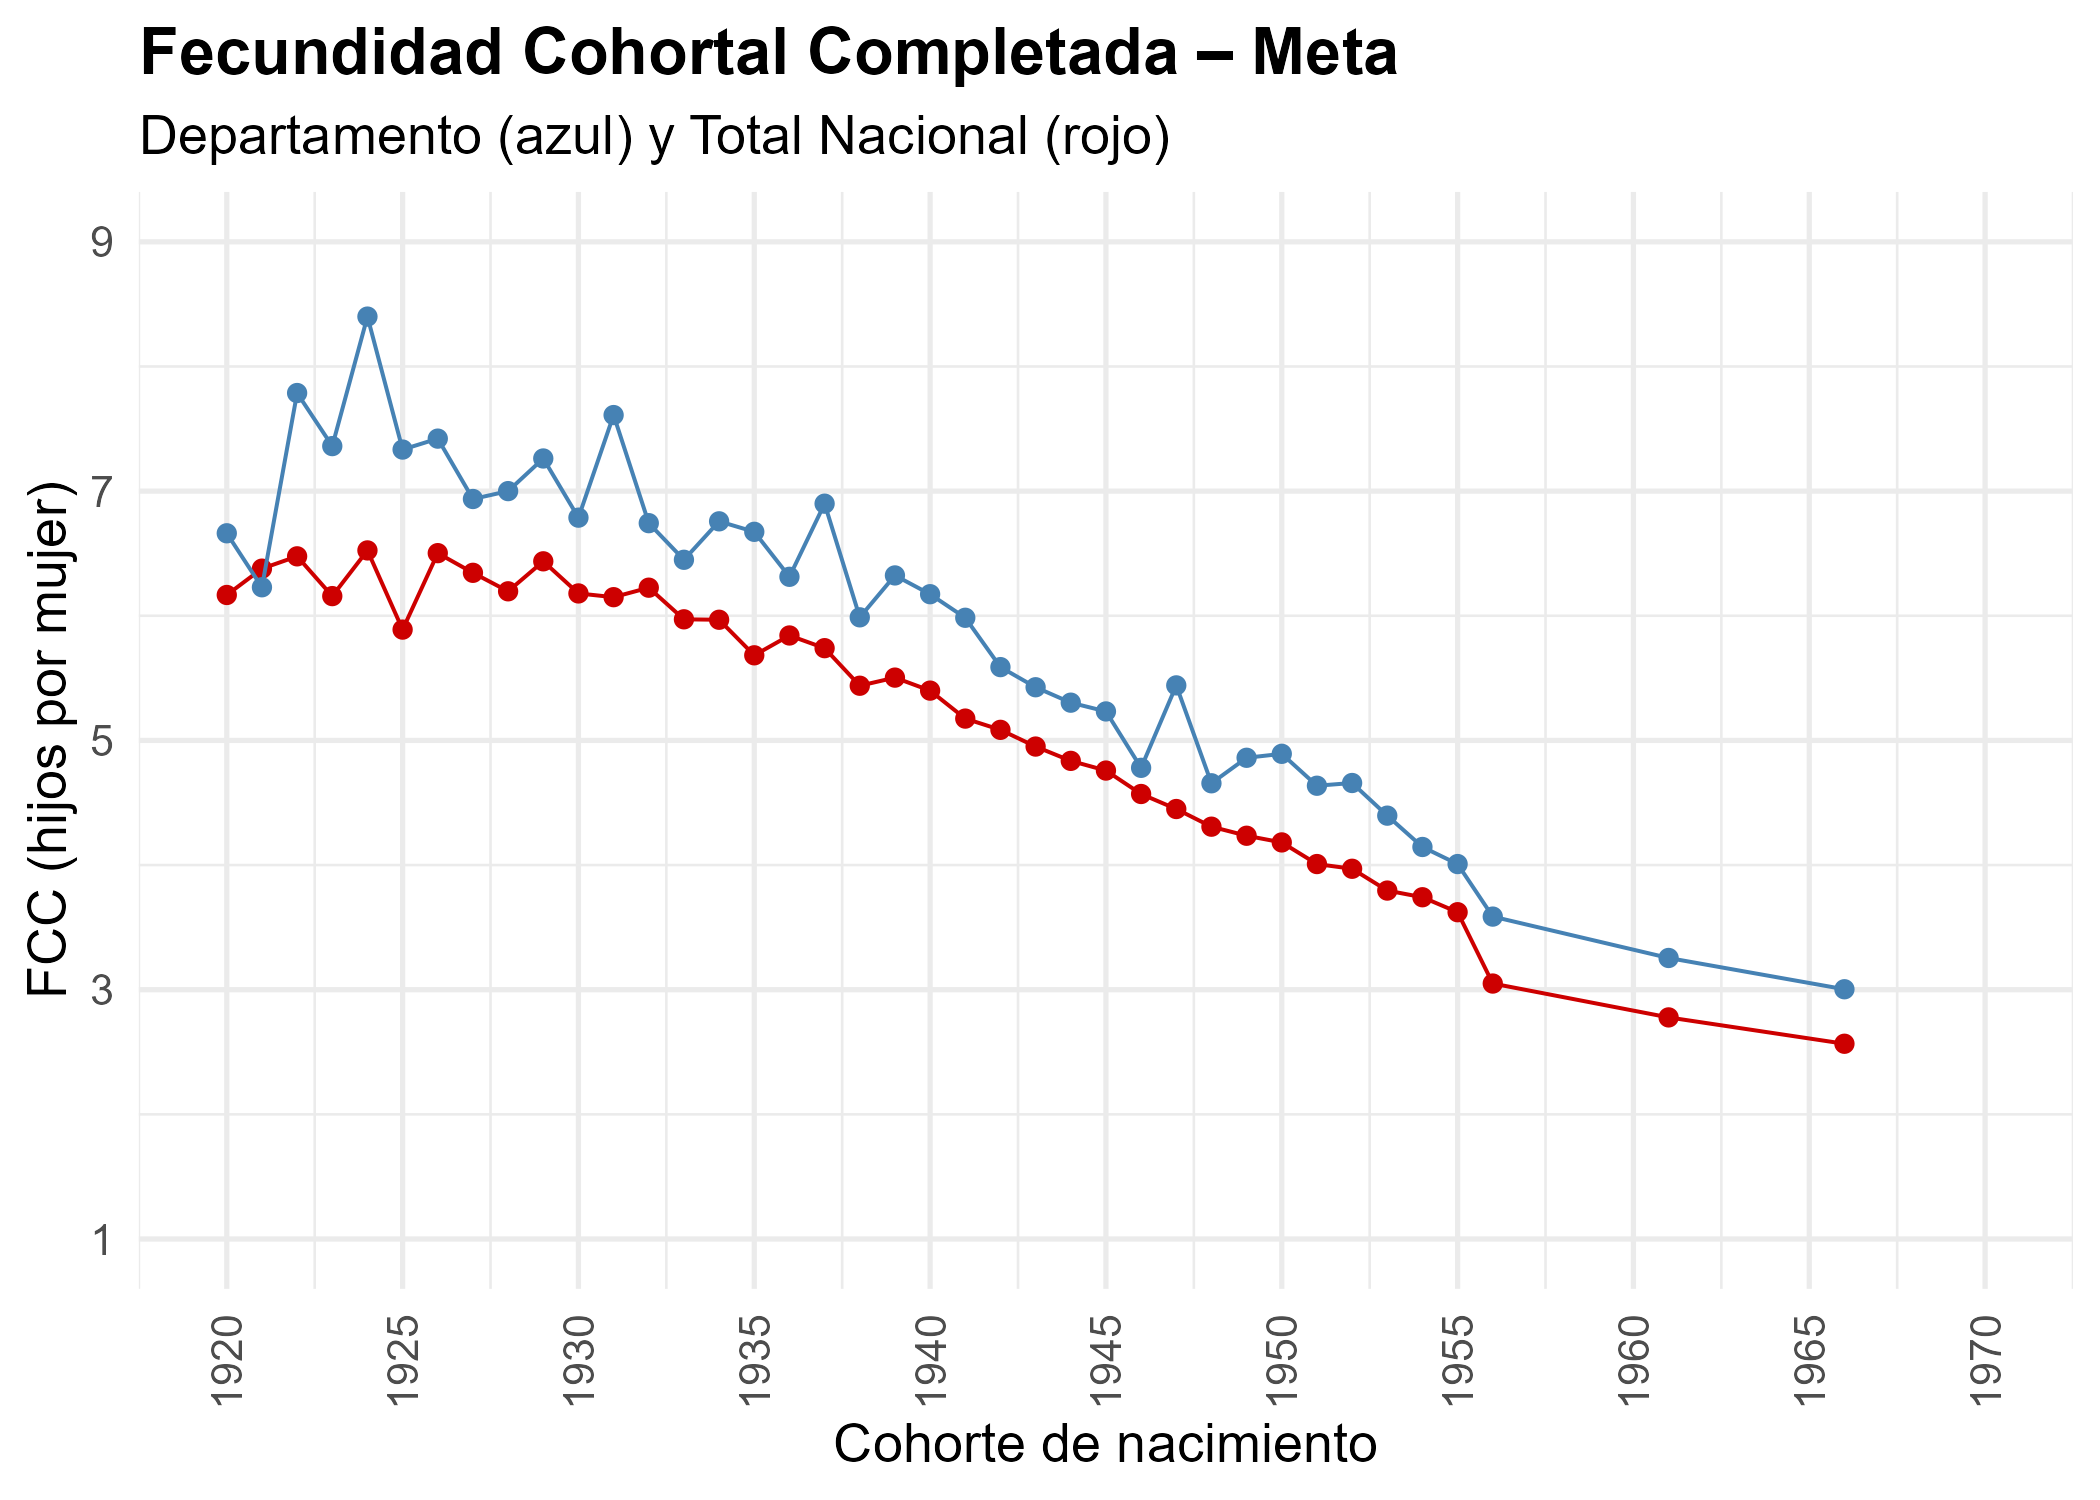
\includegraphics[width=\textwidth]{fcc_departamental/FCC_Meta_vs_National.png}
\column{0.5\textwidth}\centering
{\small Condicional (madres)}\\
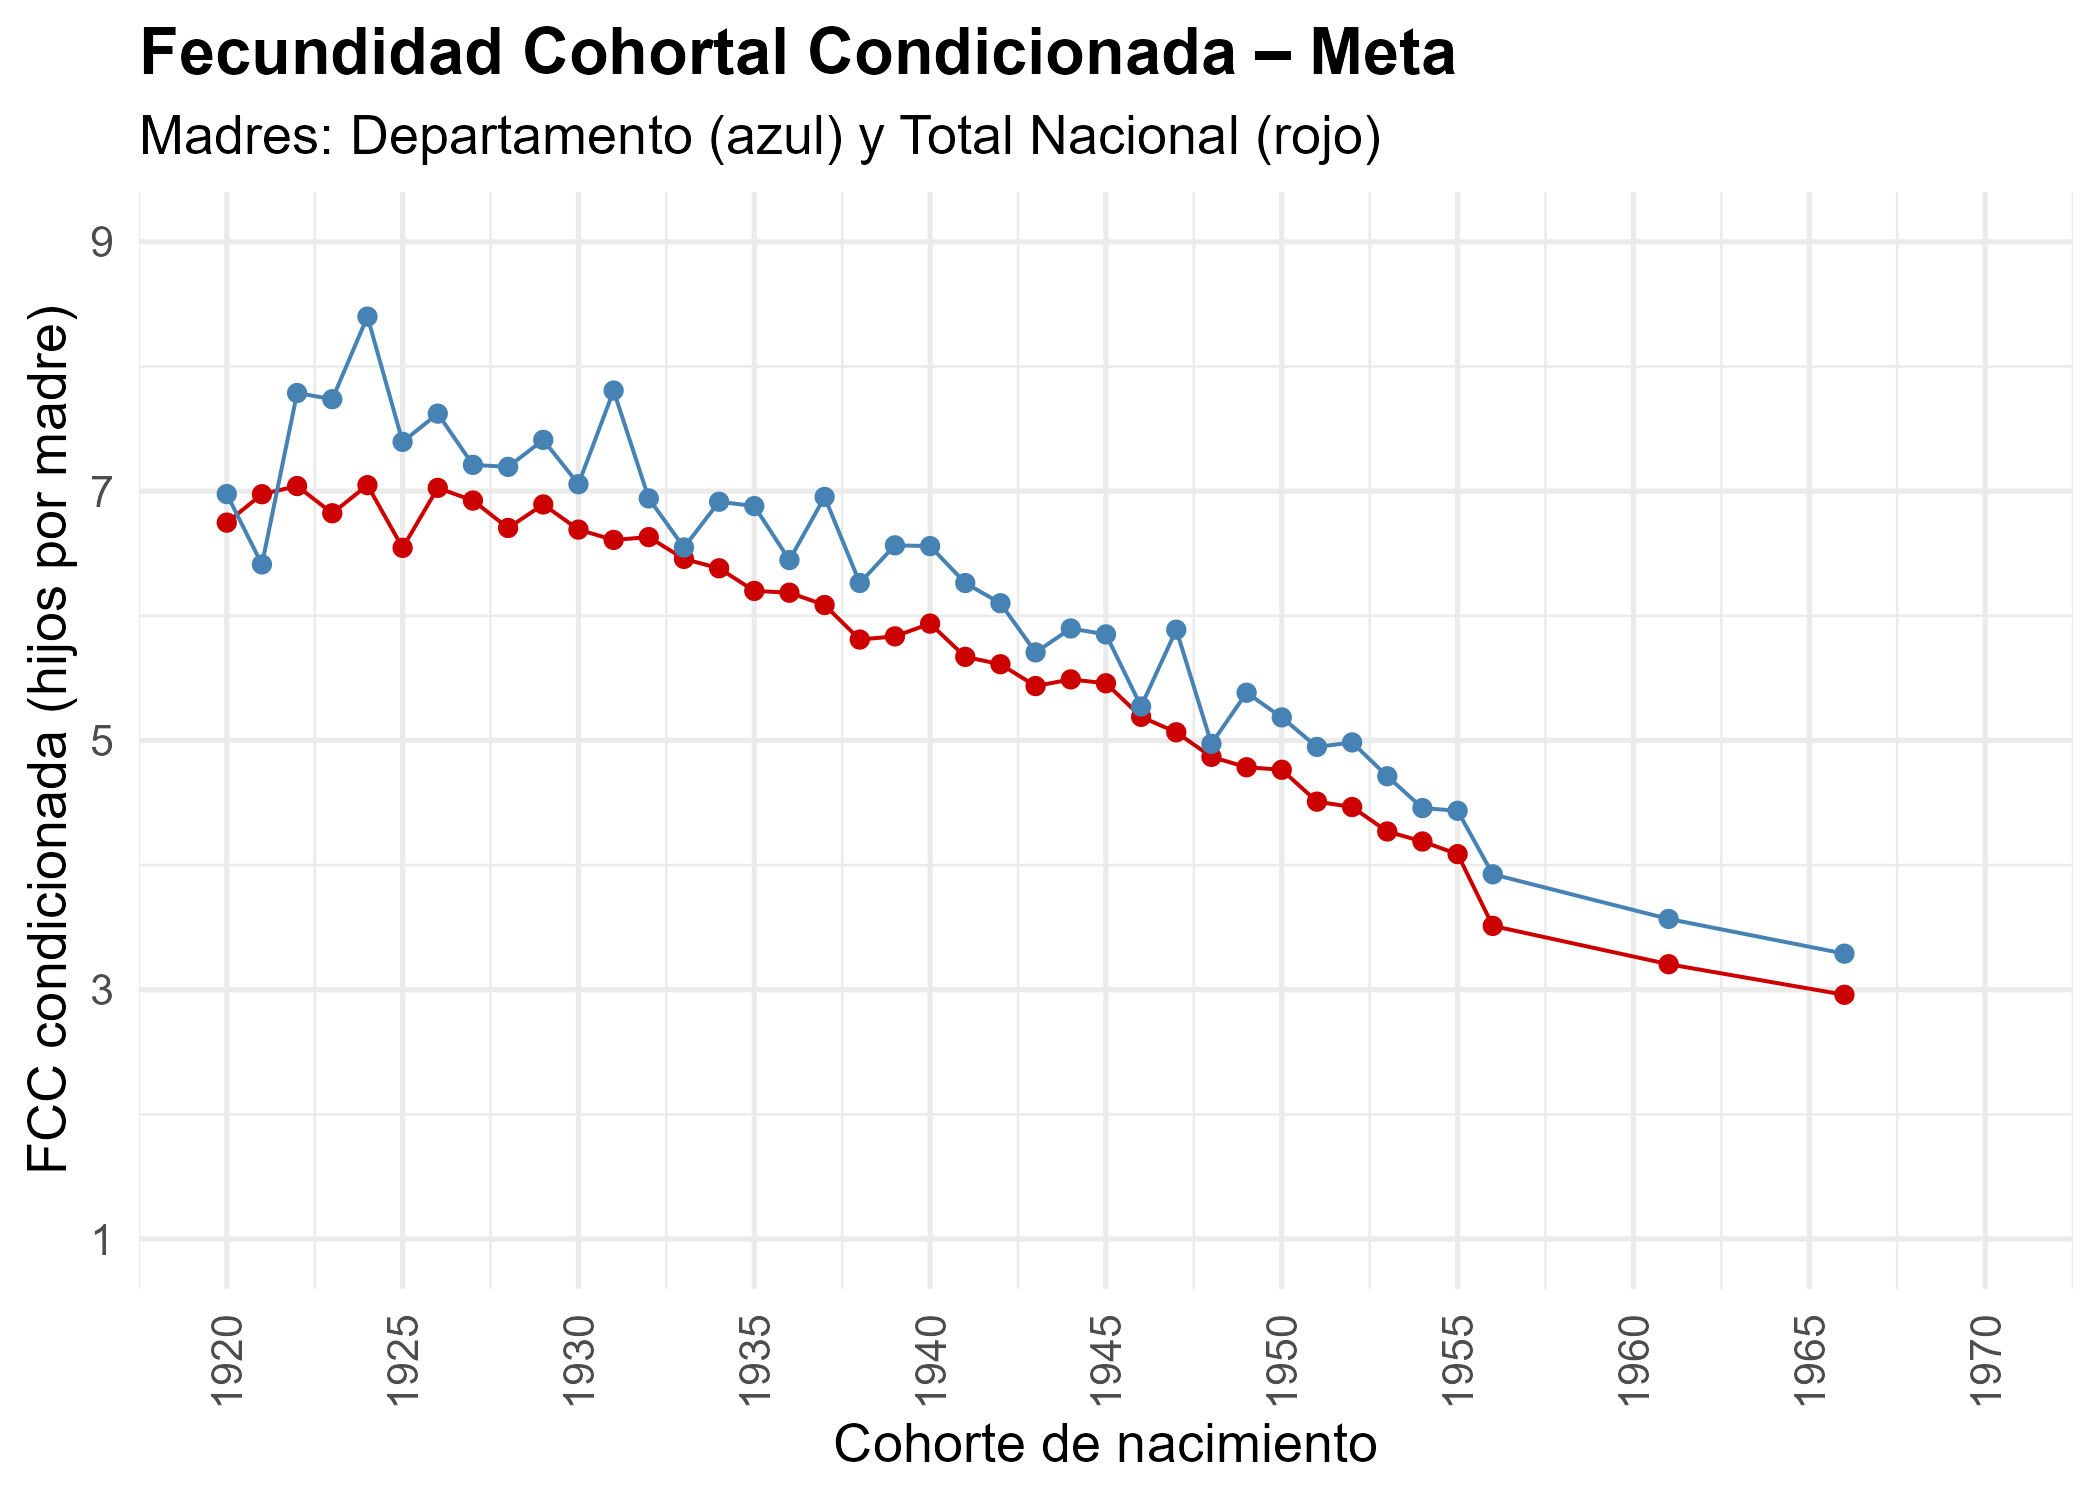
\includegraphics[width=\textwidth]{fcc_departamental/FCC_cond_Meta_vs_National.png}
\end{columns}
\end{frame}
\begin{frame}{FCC: Nariño}
\begin{columns}
\column{0.5\textwidth}\centering
{\small Todas las mujeres}\\
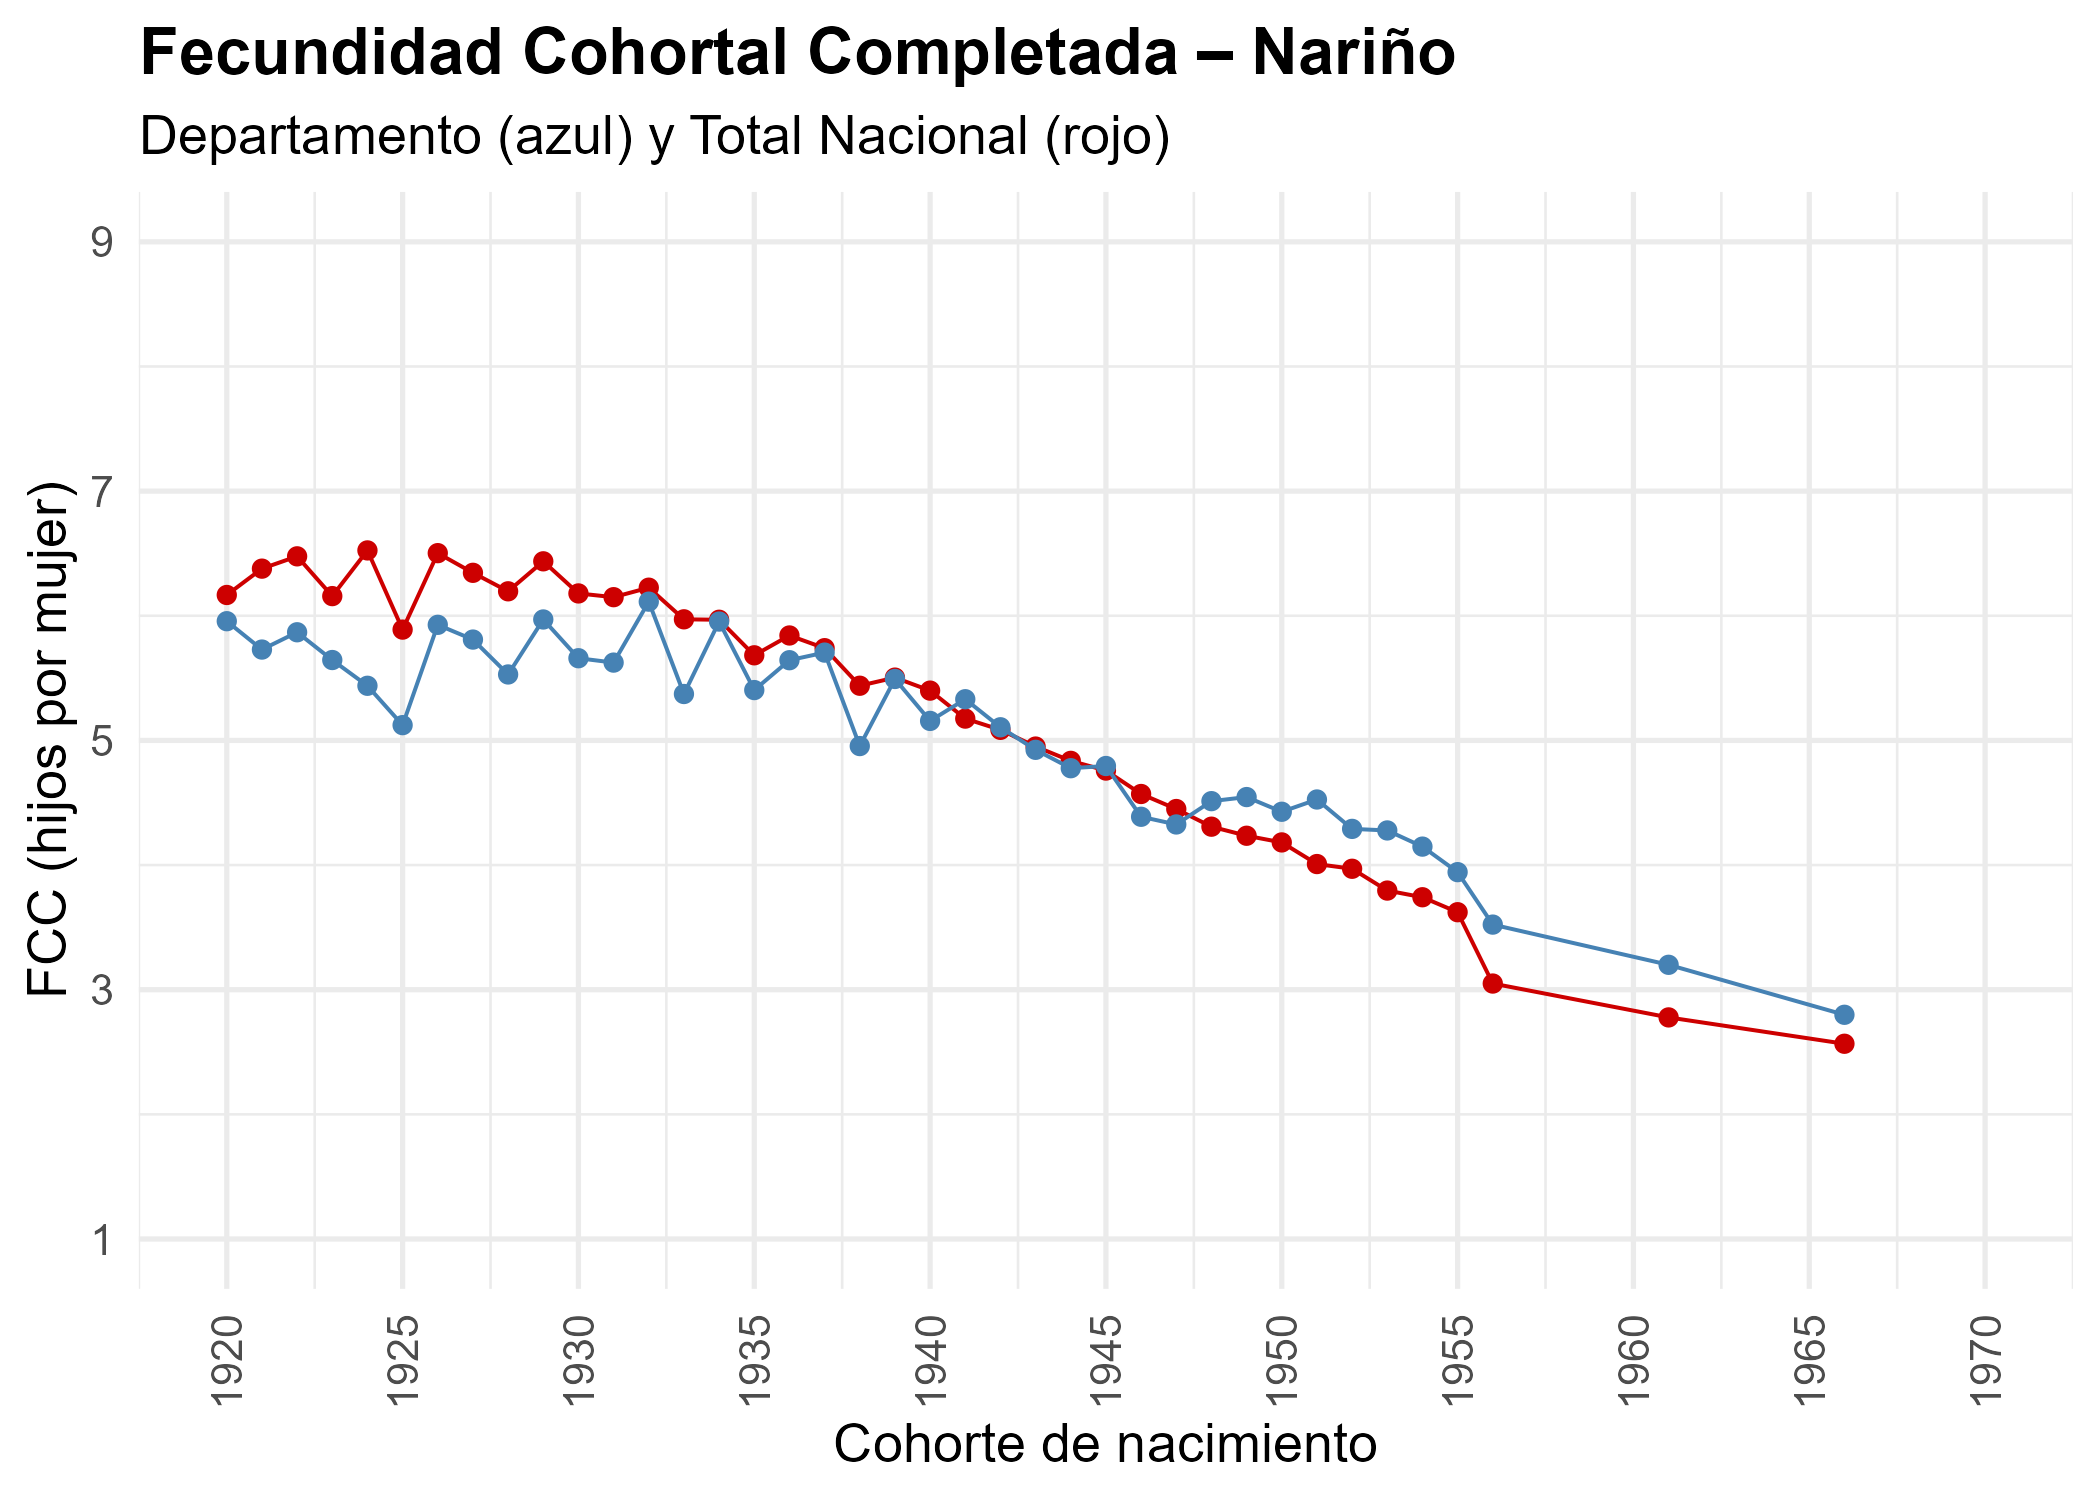
\includegraphics[width=\textwidth]{fcc_departamental/FCC_Nariño_vs_National.png}
\column{0.5\textwidth}\centering
{\small Condicional (madres)}\\
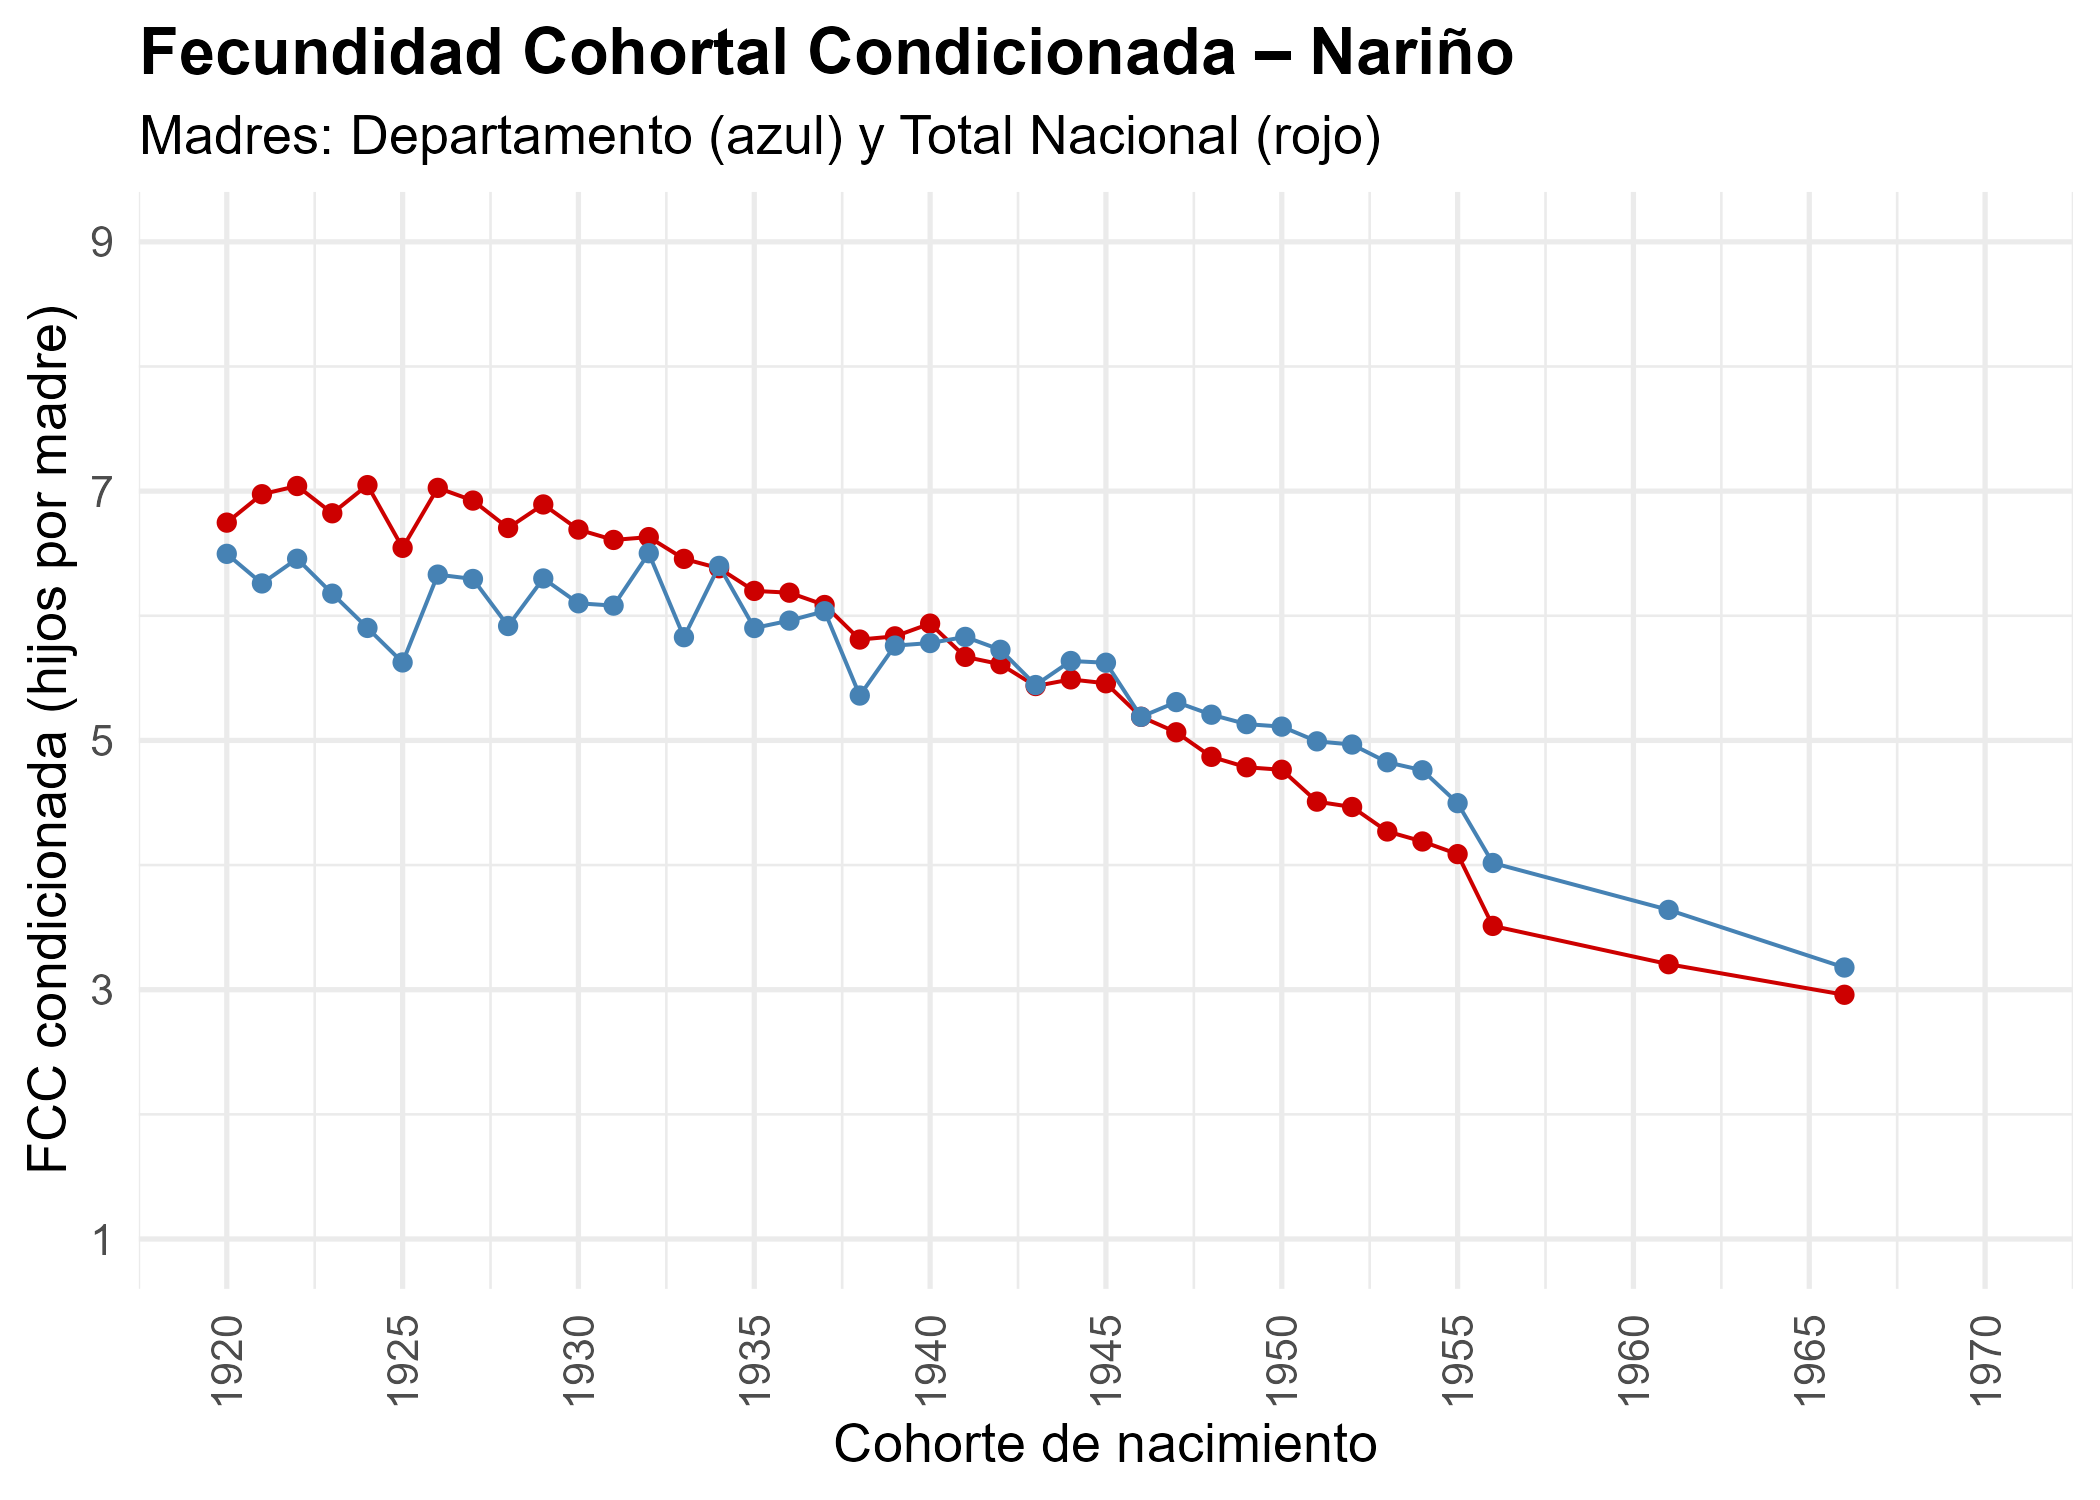
\includegraphics[width=\textwidth]{fcc_departamental/FCC_cond_Nariño_vs_National.png}
\end{columns}
\end{frame}
\begin{frame}{FCC: Putumayo}
\begin{columns}
\column{0.5\textwidth}\centering
{\small Todas las mujeres}\\
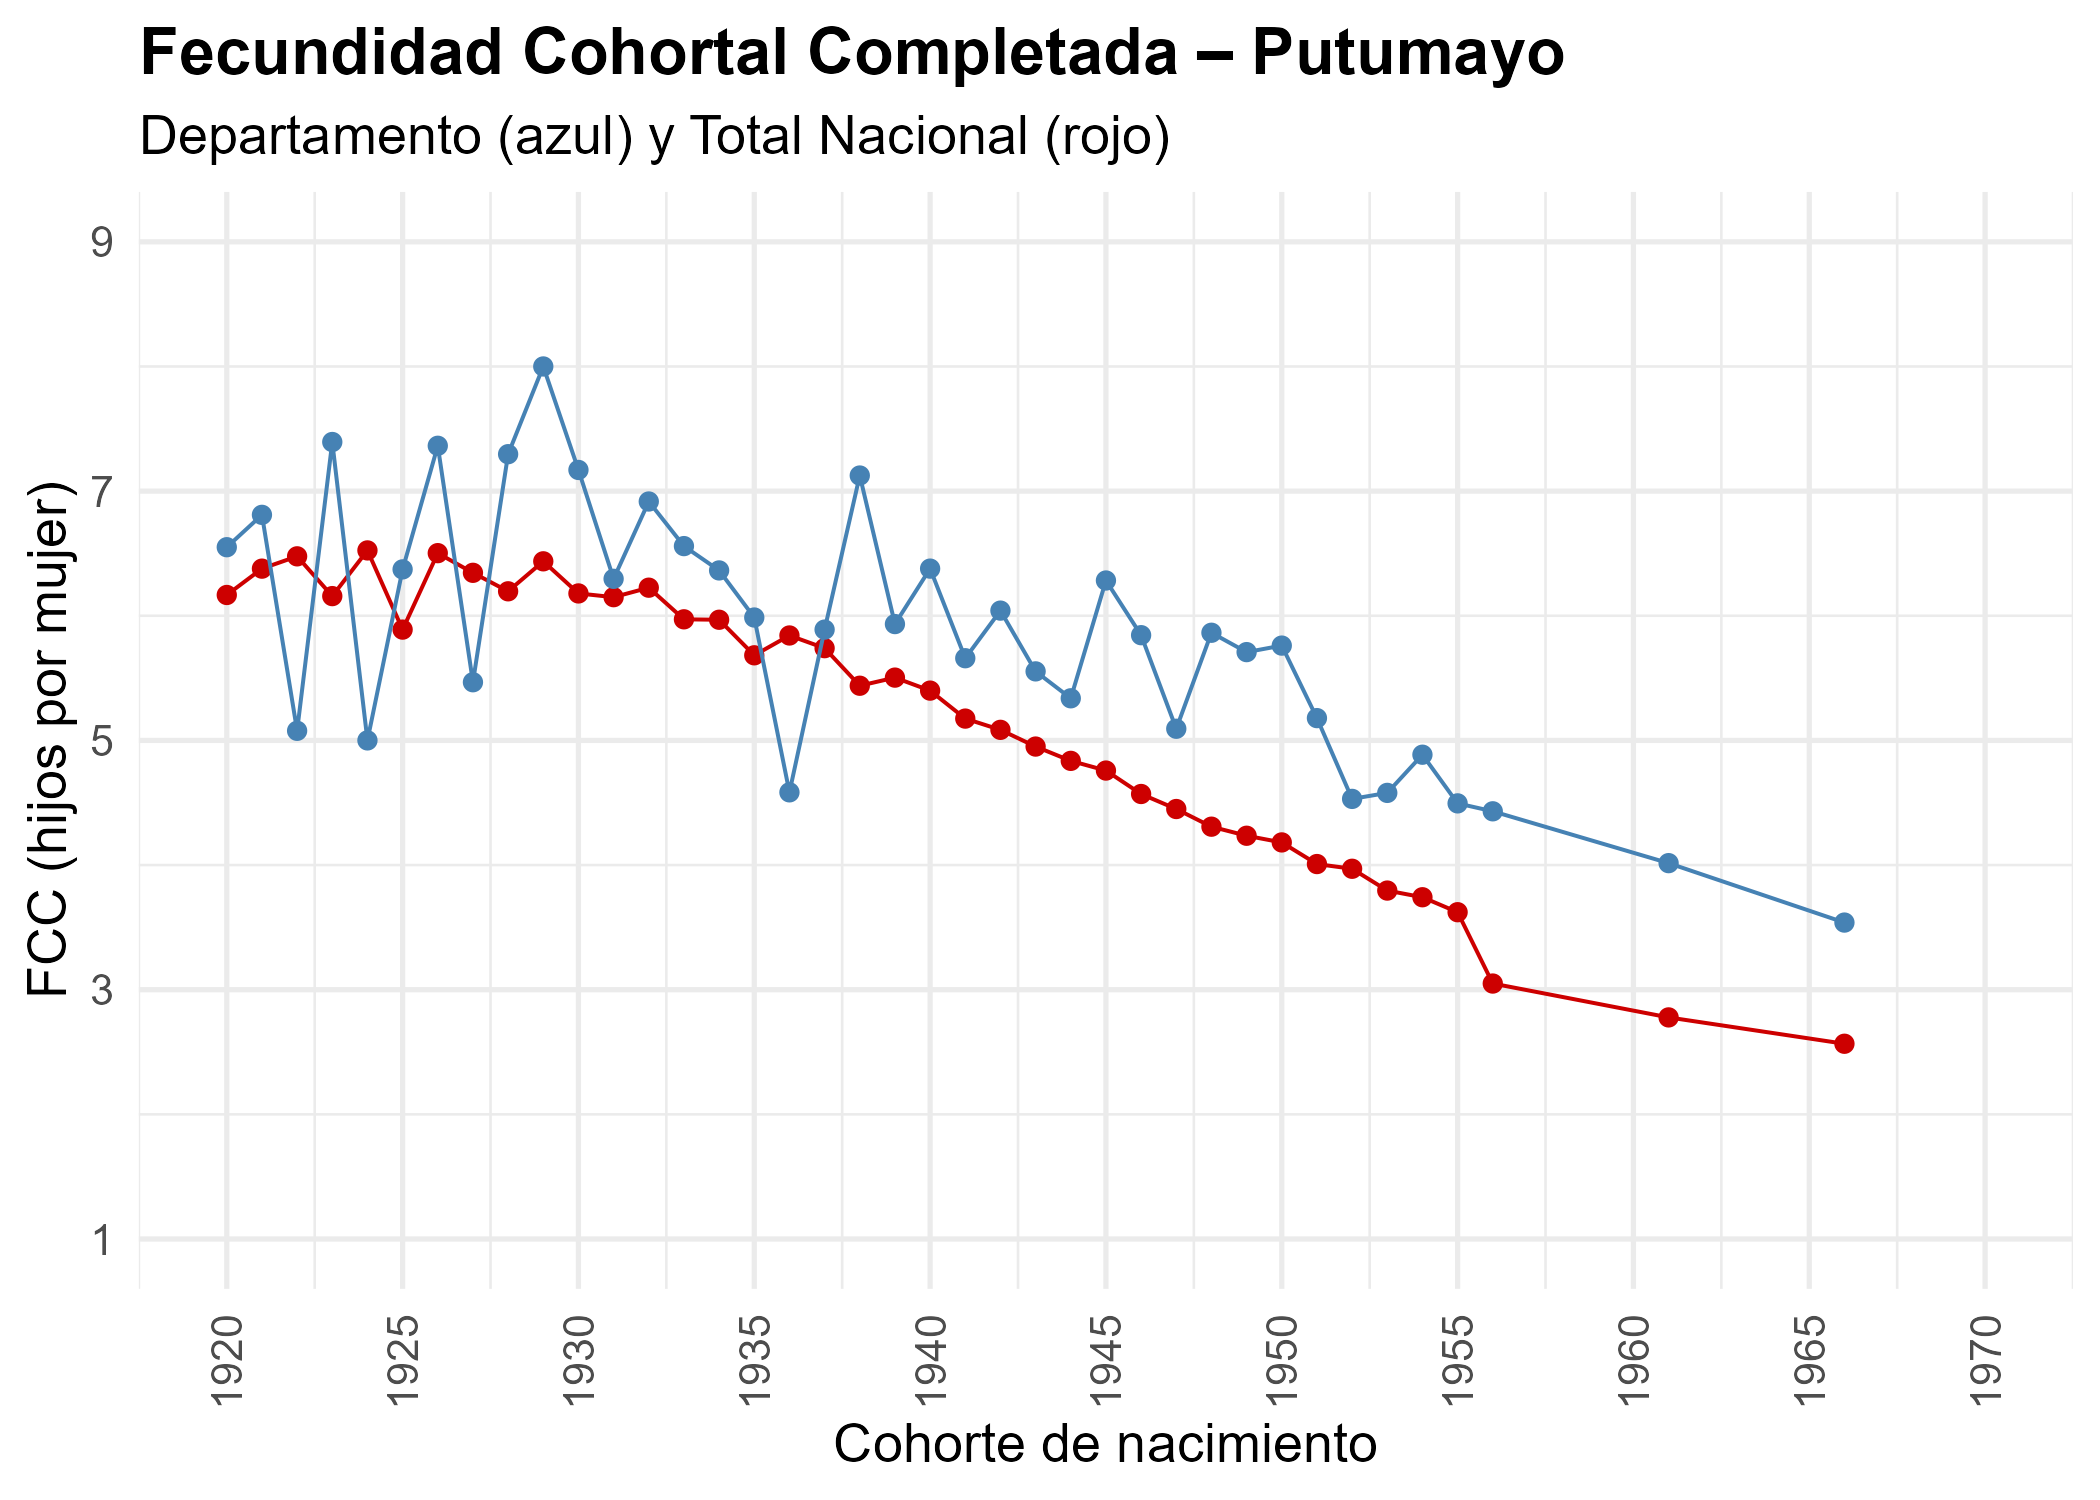
\includegraphics[width=\textwidth]{fcc_departamental/FCC_Putumayo_vs_National.png}
\column{0.5\textwidth}\centering
{\small Condicional (madres)}\\
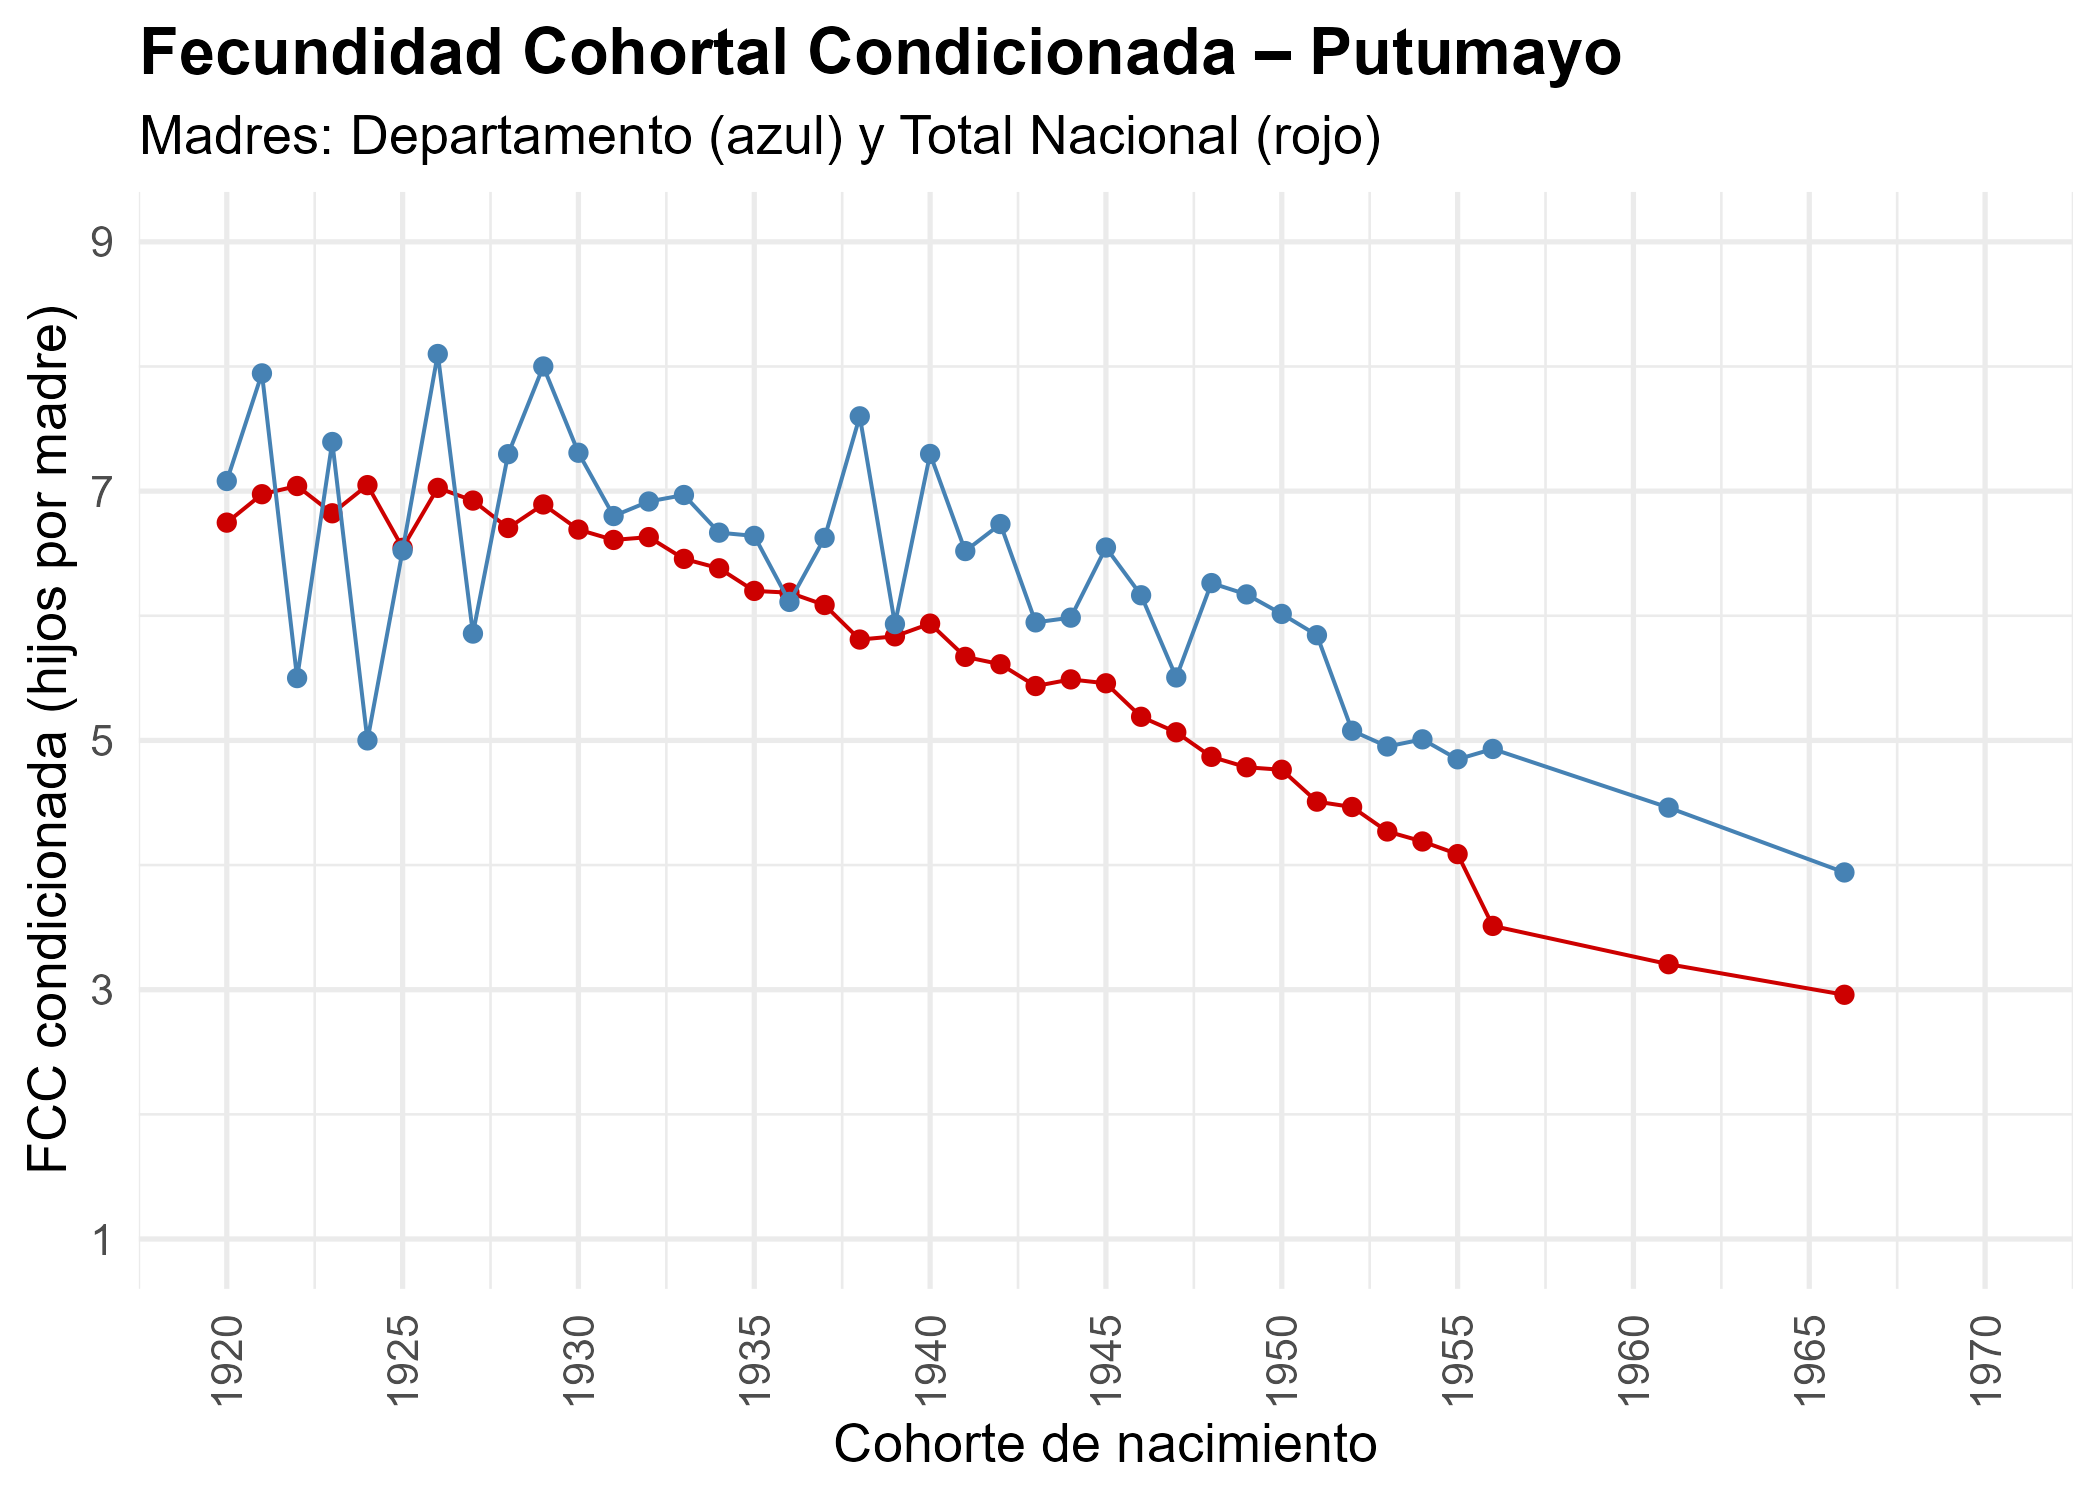
\includegraphics[width=\textwidth]{fcc_departamental/FCC_cond_Putumayo_vs_National.png}
\end{columns}
\end{frame}
\begin{frame}{FCC: San Andrés}
\begin{columns}
\column{0.5\textwidth}\centering
{\small Todas las mujeres}\\
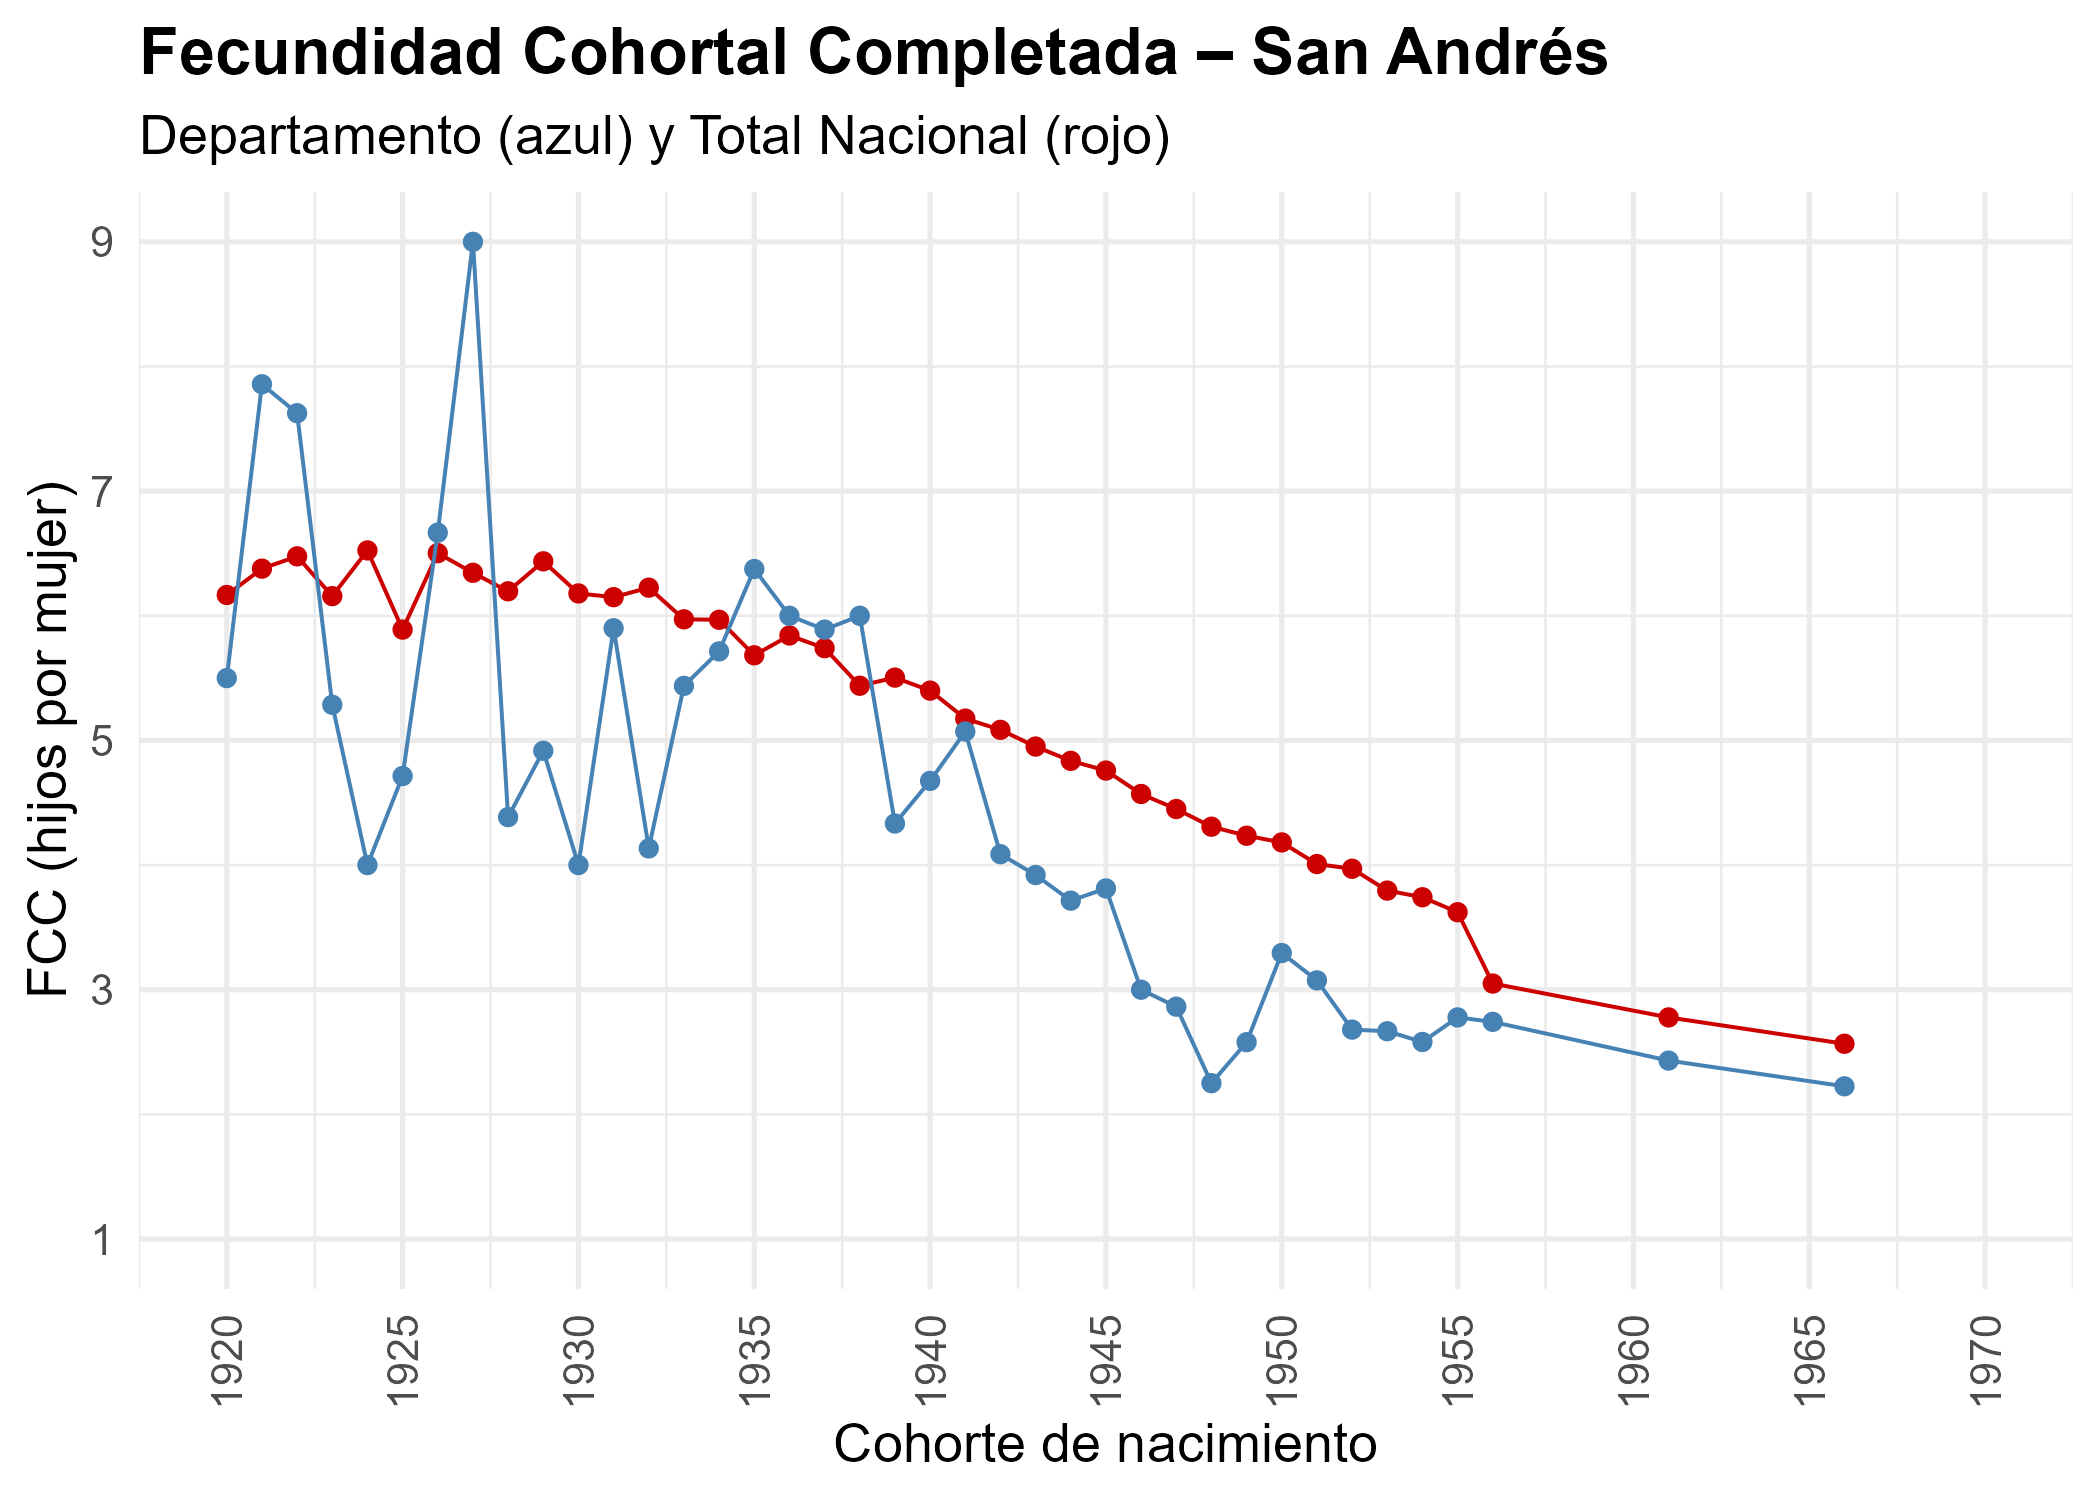
\includegraphics[width=\textwidth]{fcc_departamental/FCC_San Andrés_vs_National.png}
\column{0.5\textwidth}\centering
{\small Condicional (madres)}\\
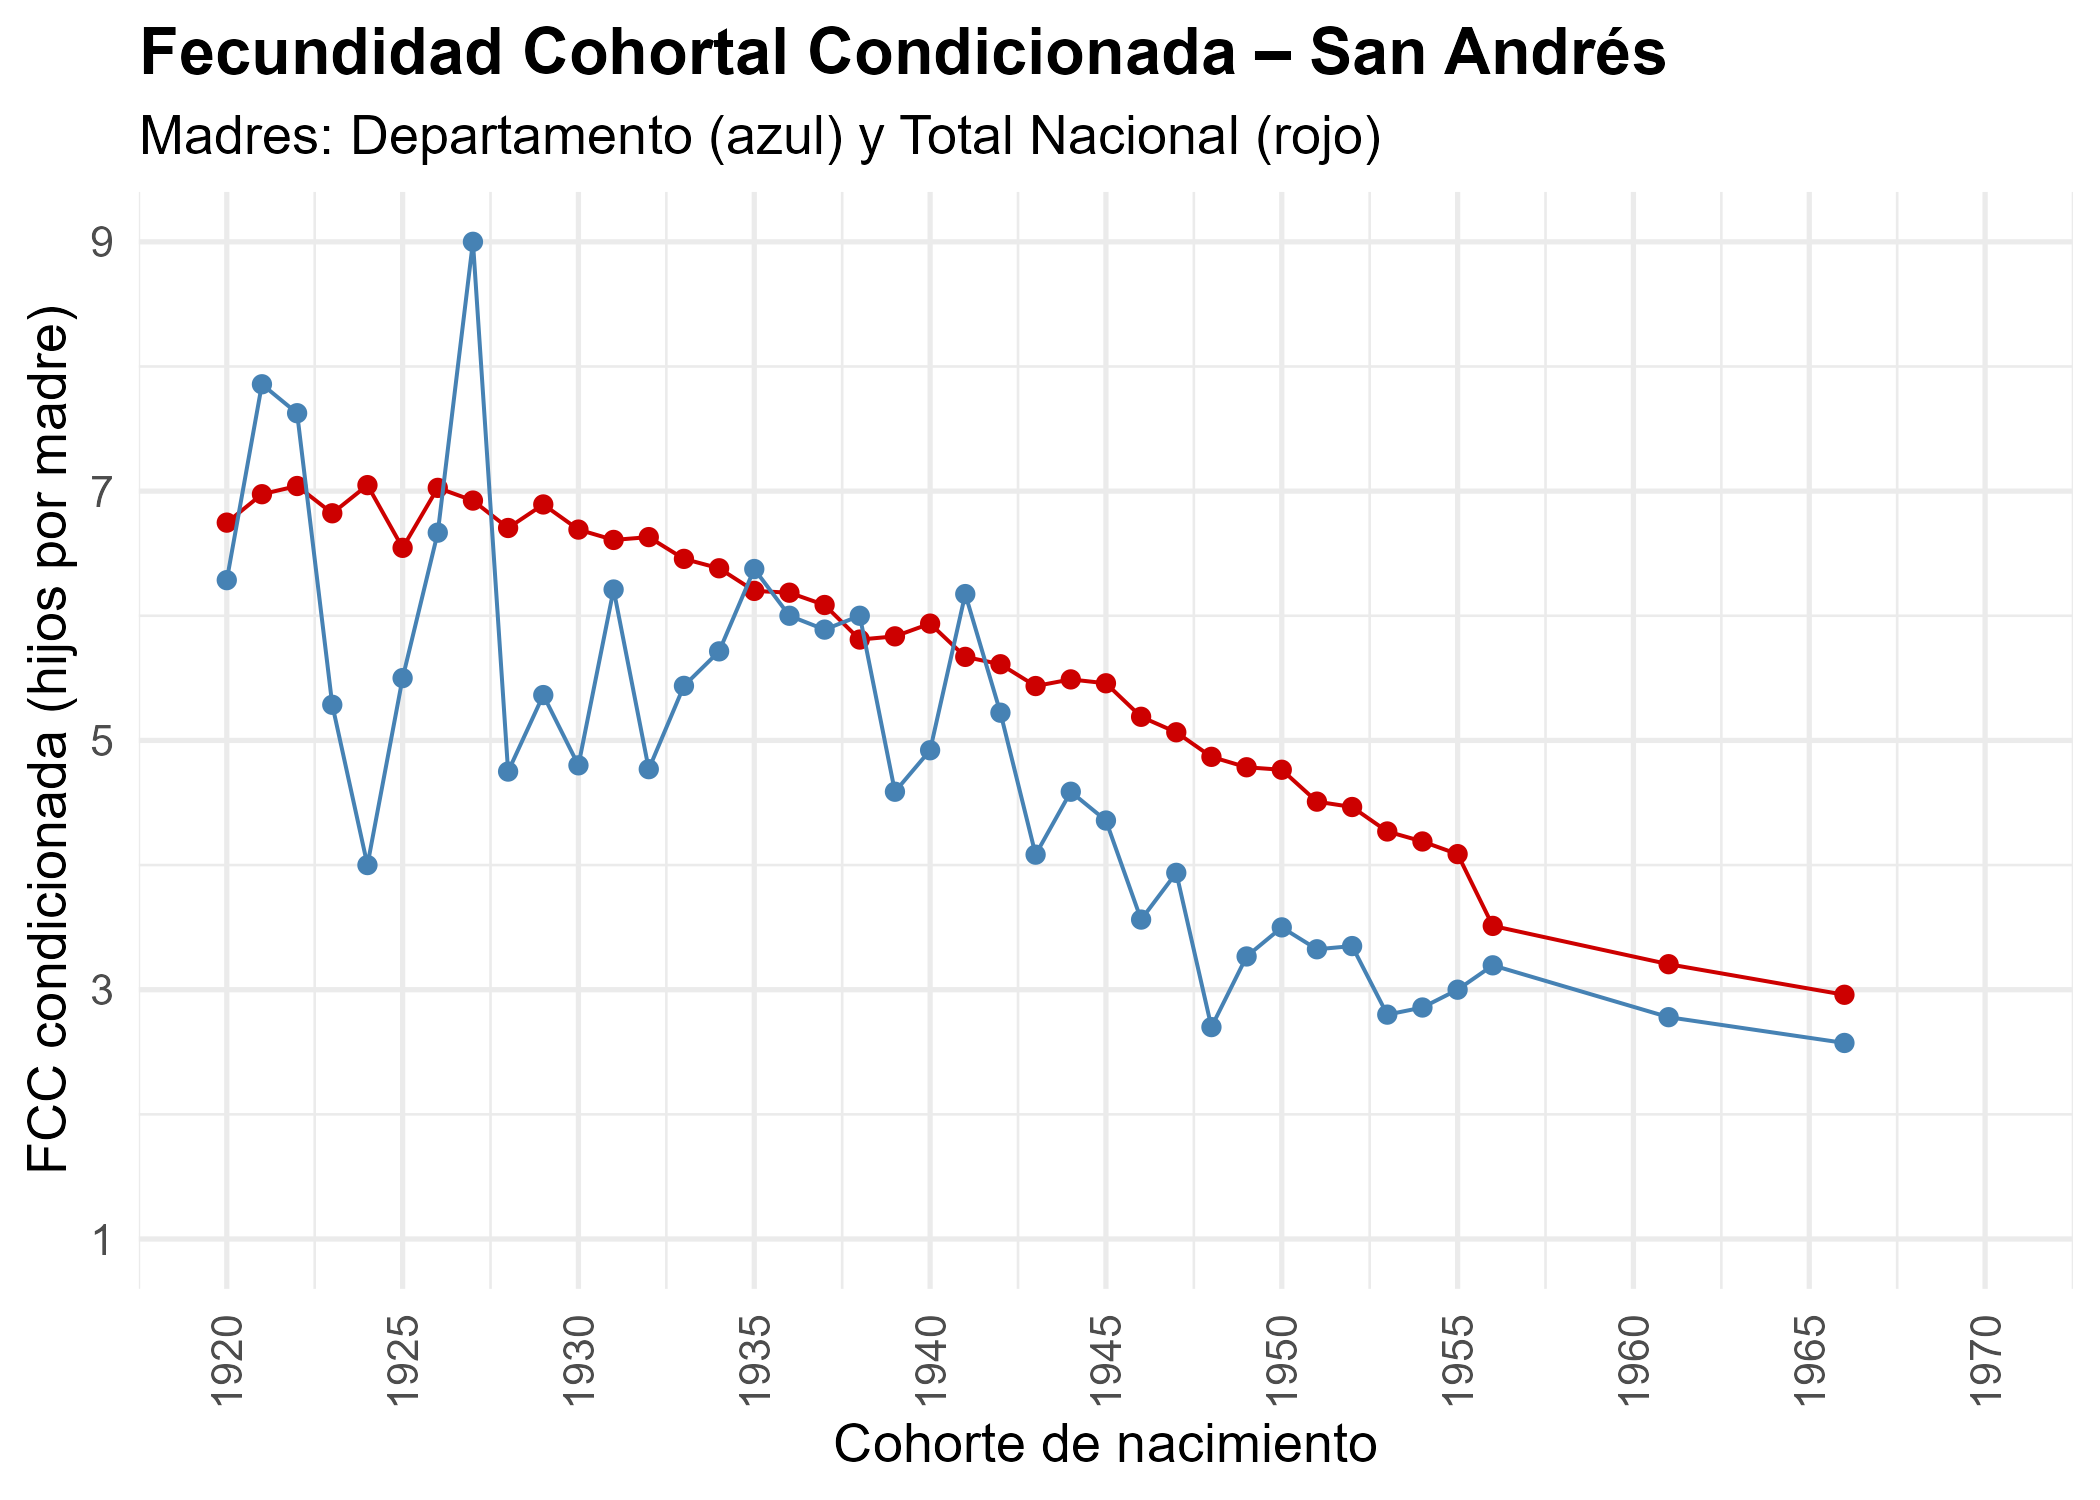
\includegraphics[width=\textwidth]{fcc_departamental/FCC_cond_San Andrés_vs_National.png}
\end{columns}
\end{frame}
\begin{frame}{FCC: Santander}
\begin{columns}
\column{0.5\textwidth}\centering
{\small Todas las mujeres}\\
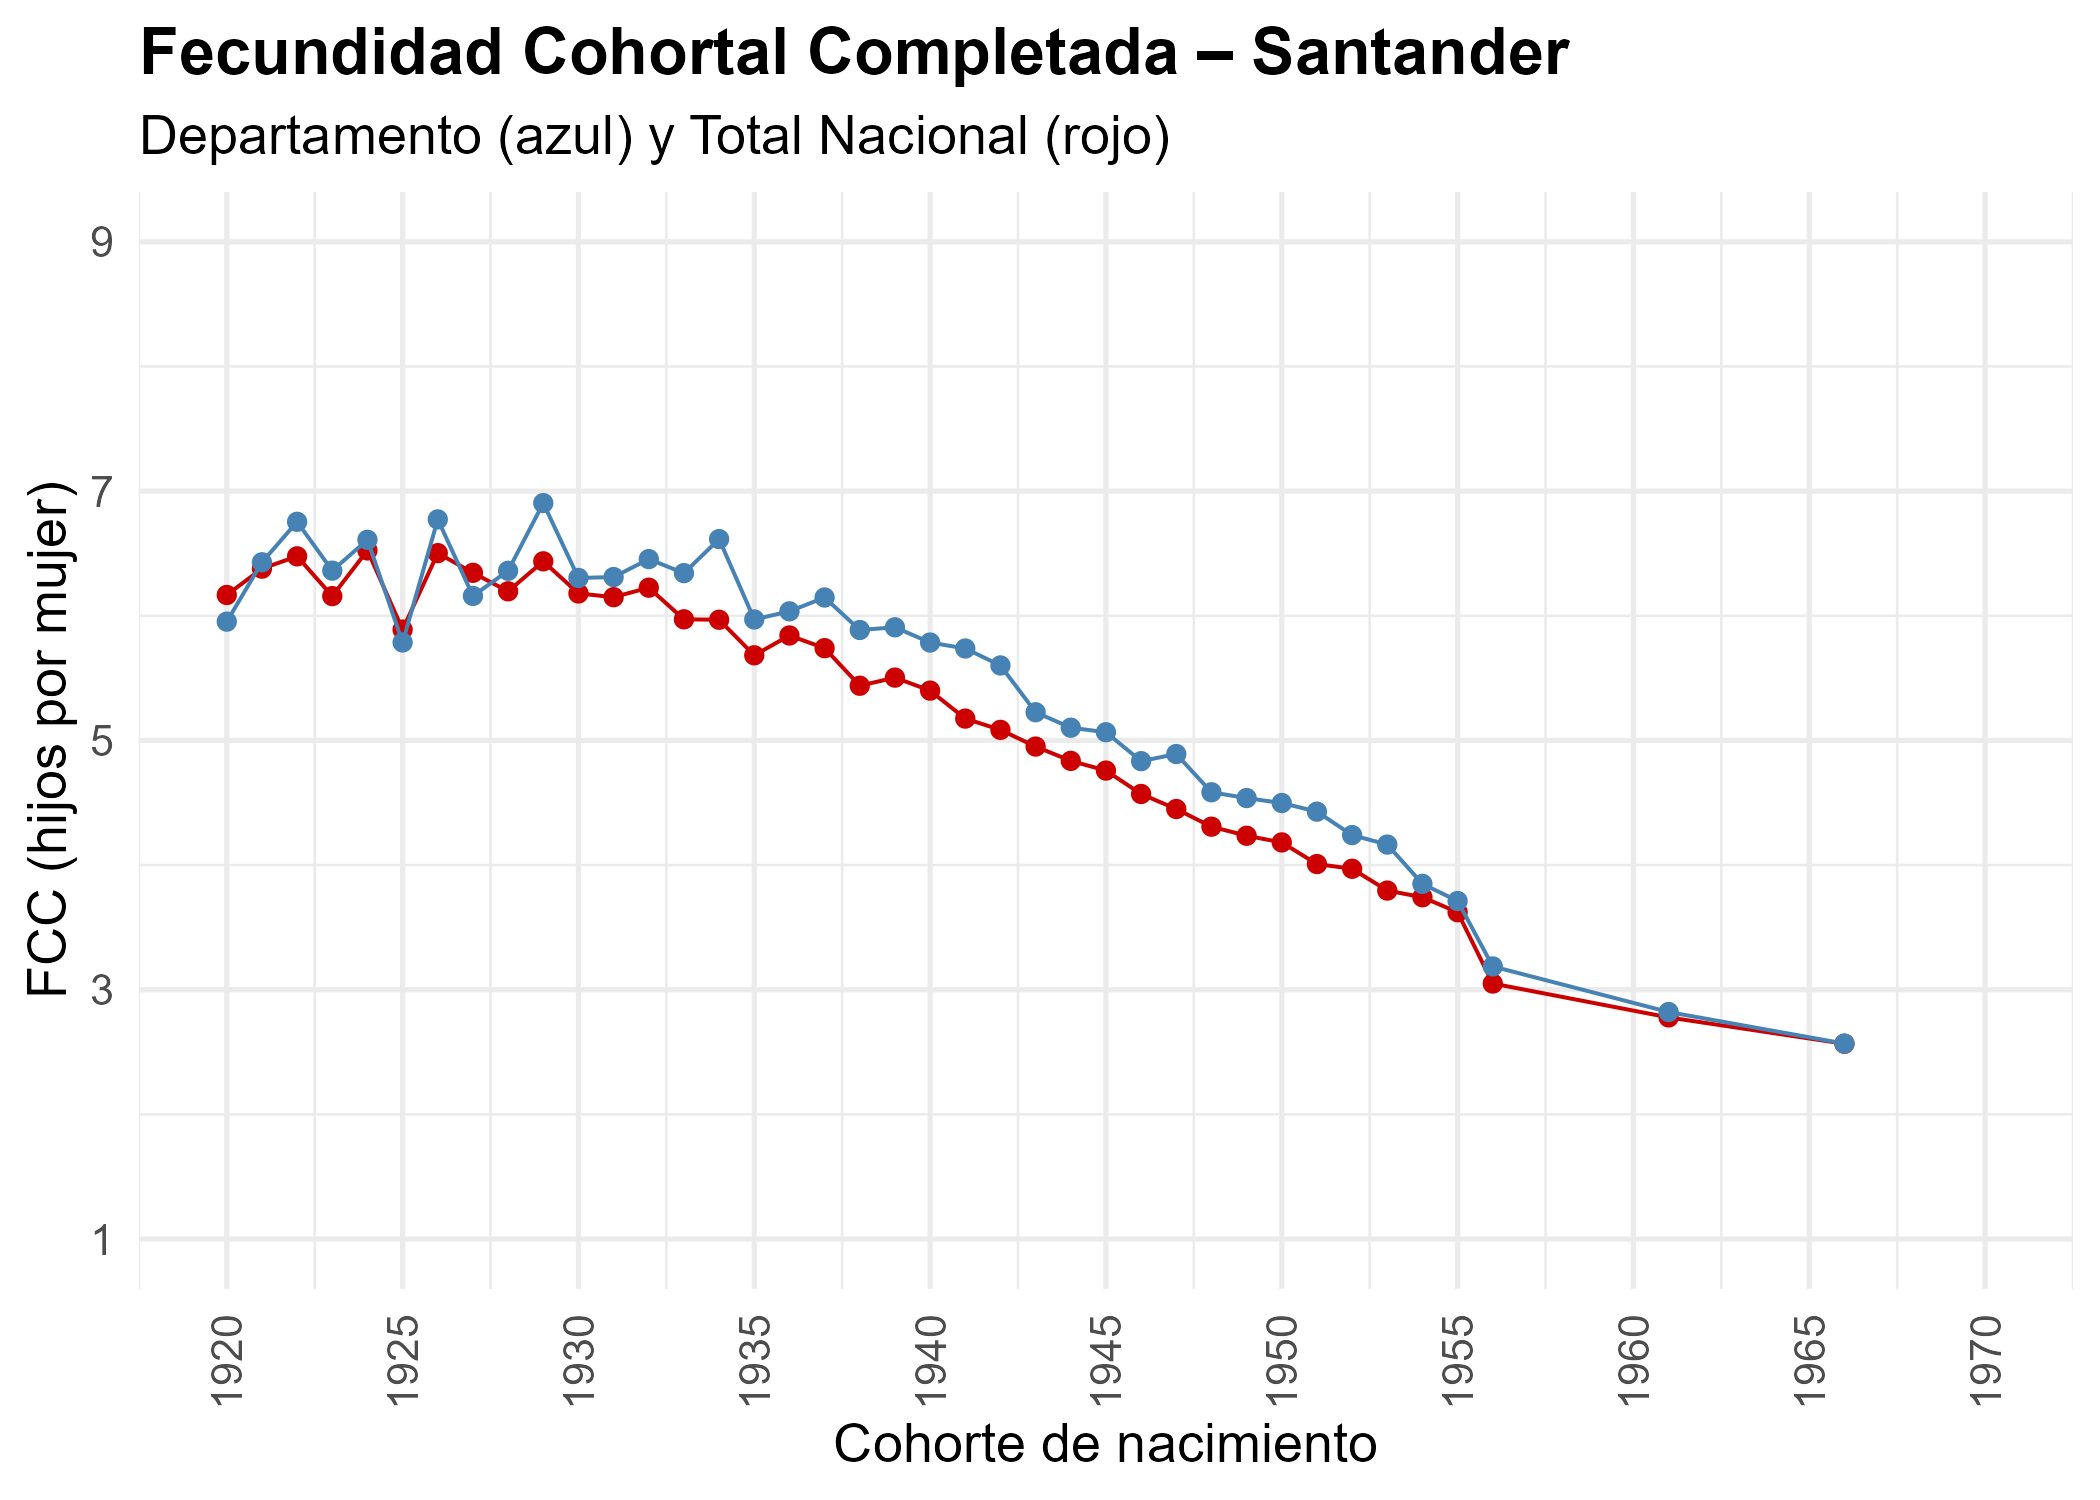
\includegraphics[width=\textwidth]{fcc_departamental/FCC_Santander_vs_National.png}
\column{0.5\textwidth}\centering
{\small Condicional (madres)}\\
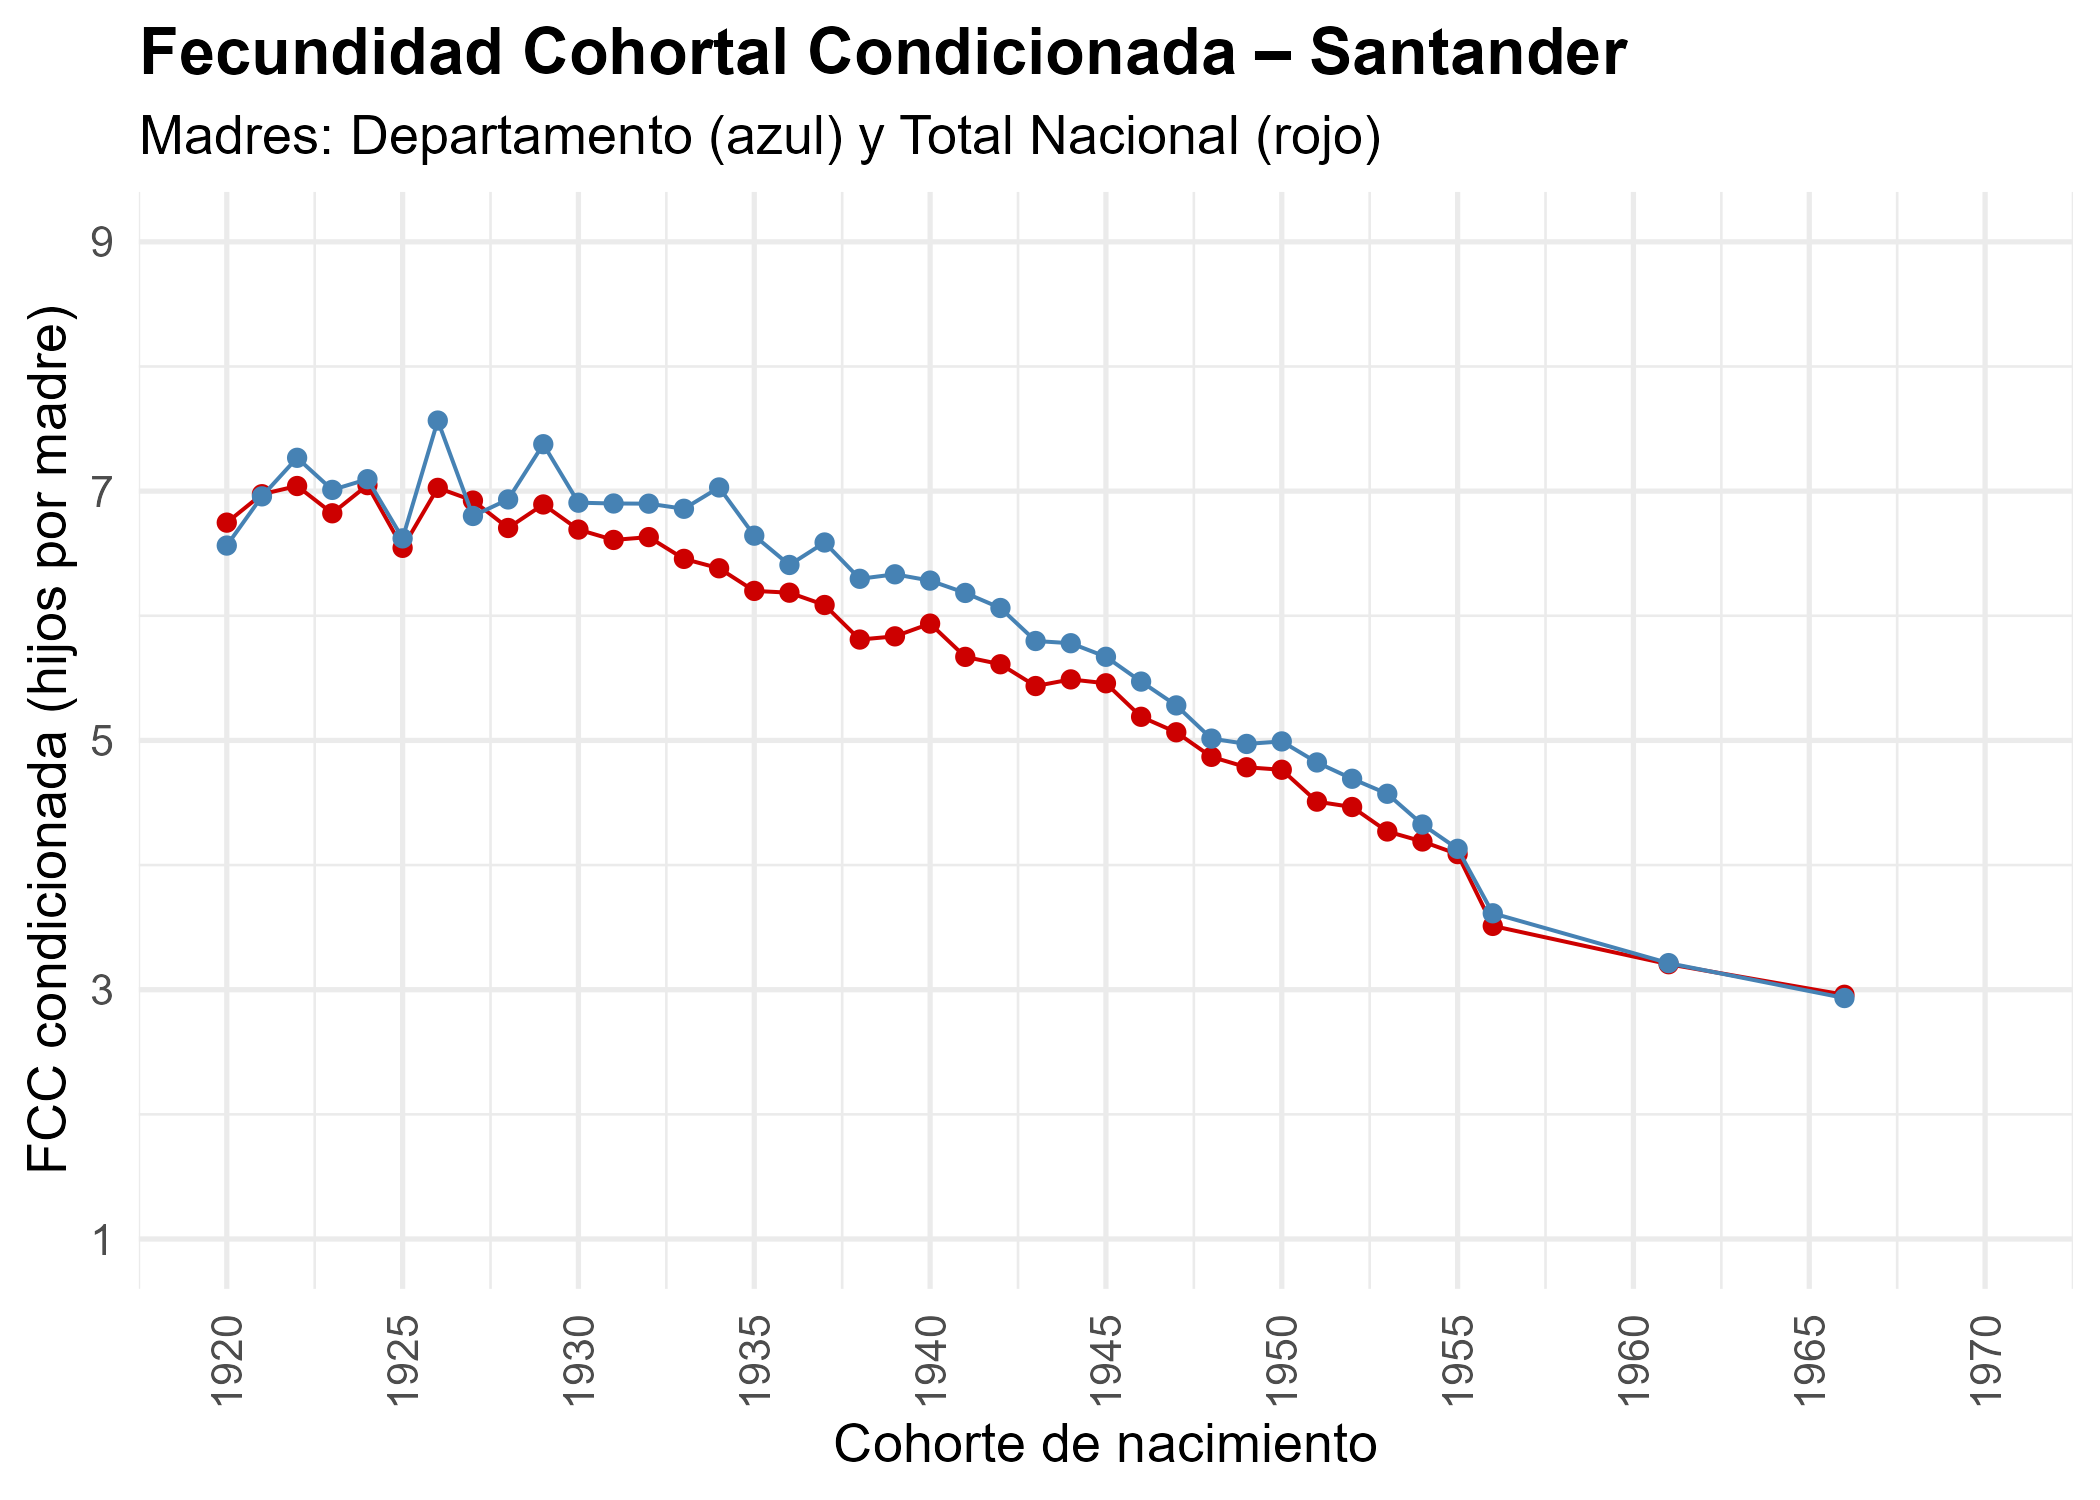
\includegraphics[width=\textwidth]{fcc_departamental/FCC_cond_Santander_vs_National.png}
\end{columns}
\end{frame}
\begin{frame}{FCC: Tolima}
\begin{columns}
\column{0.5\textwidth}\centering
{\small Todas las mujeres}\\
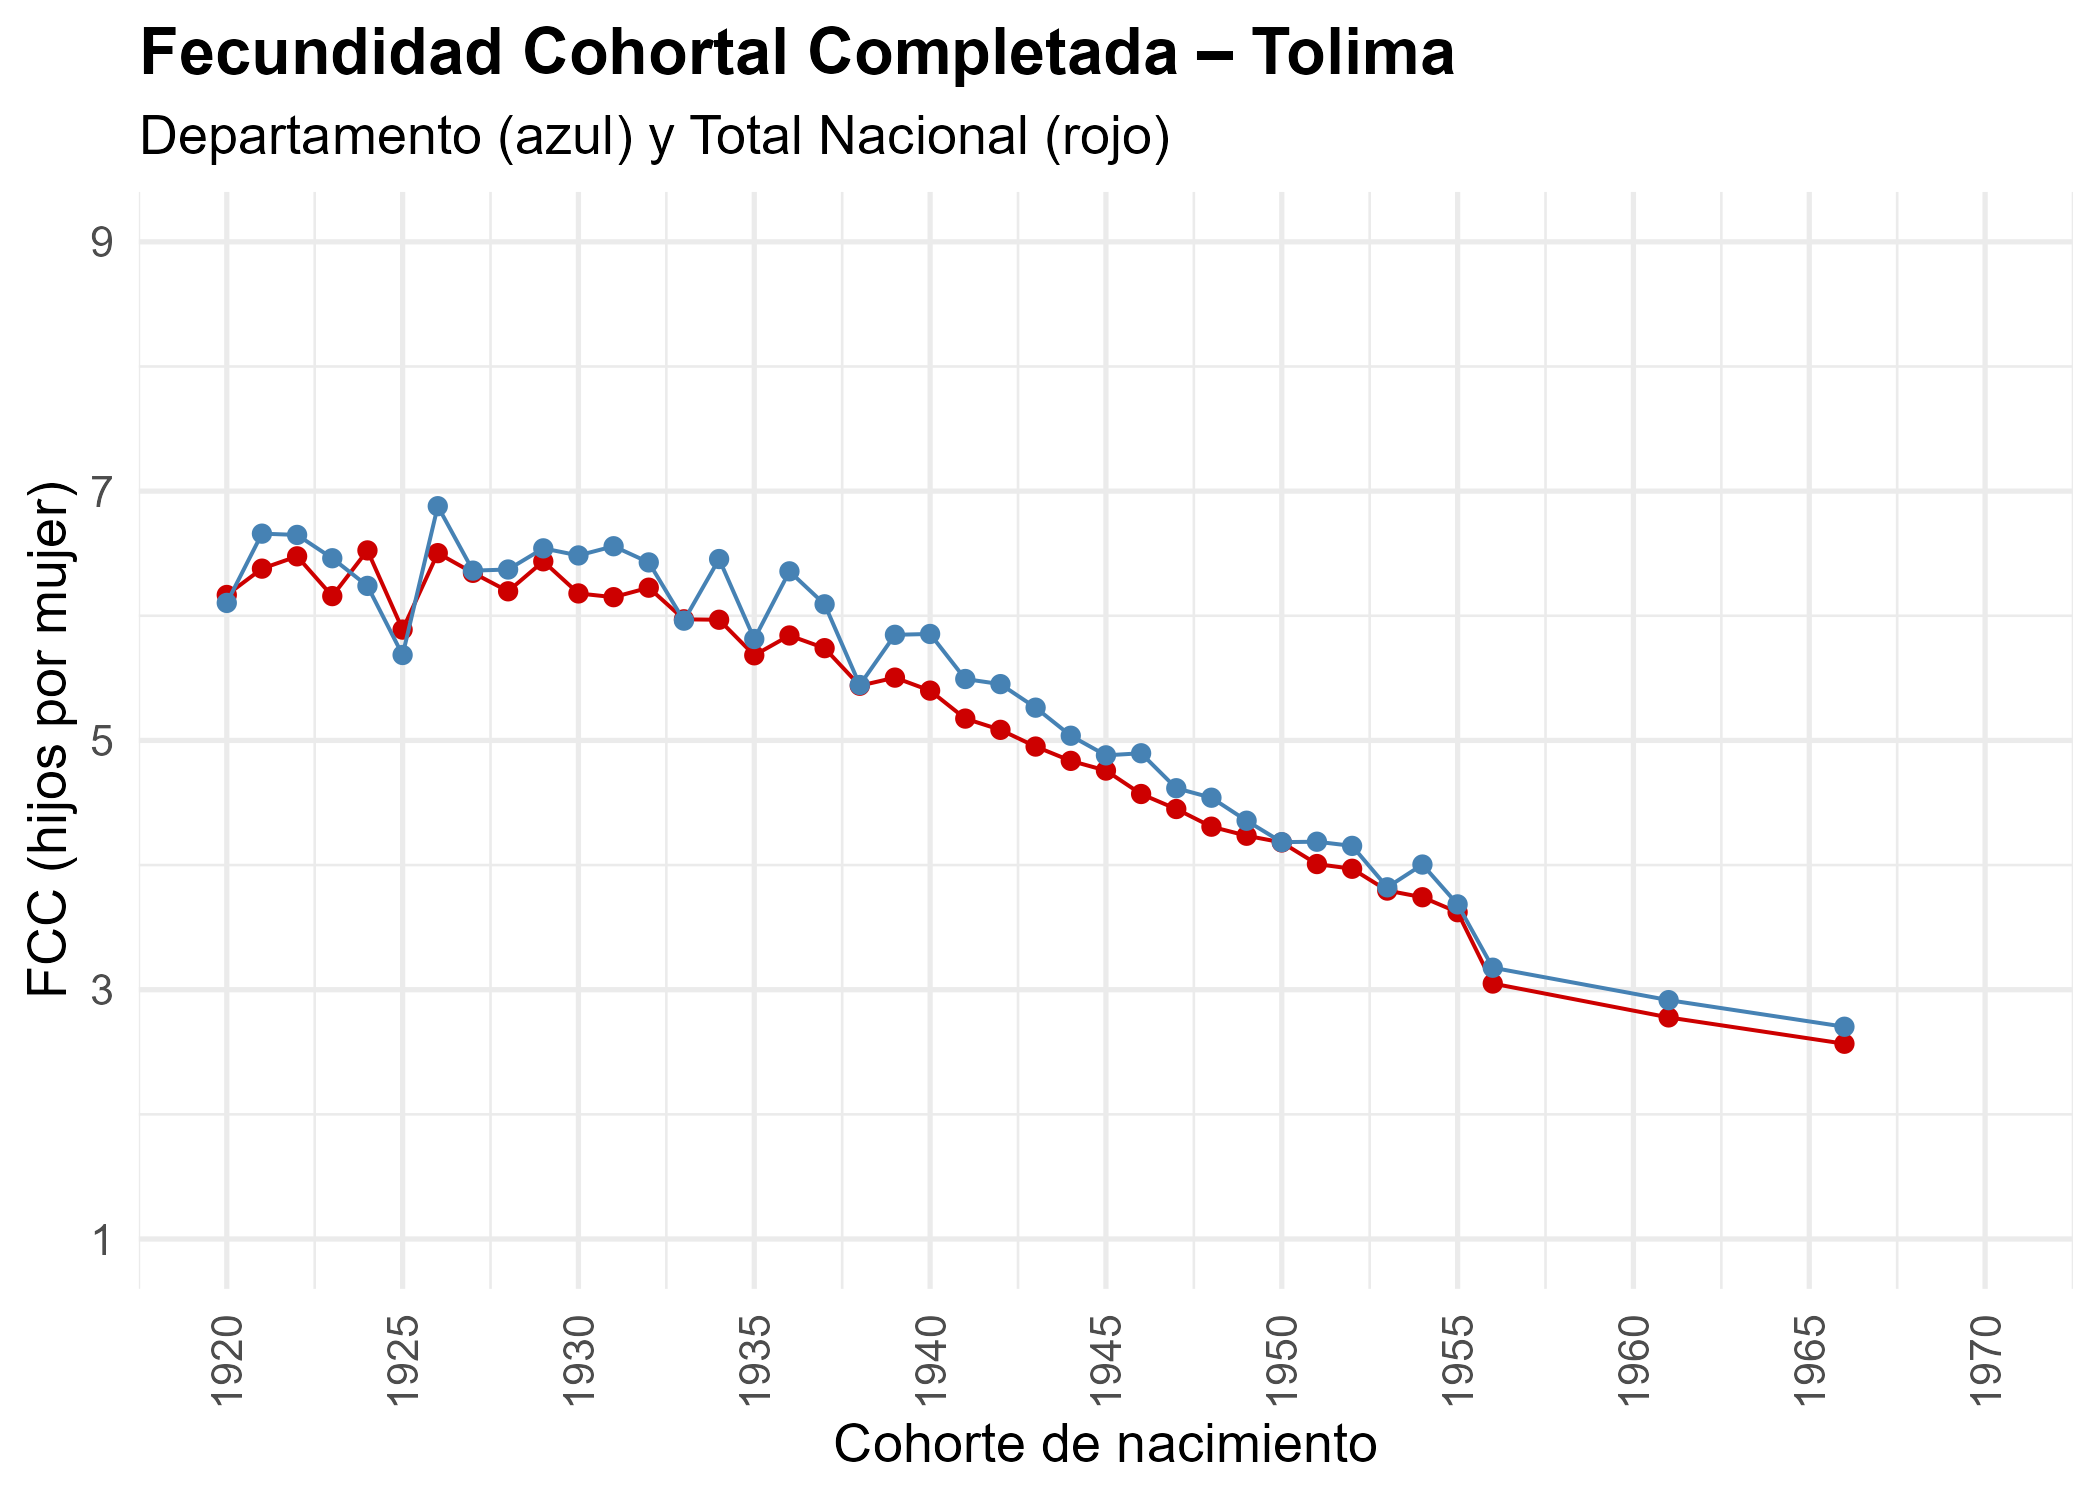
\includegraphics[width=\textwidth]{fcc_departamental/FCC_Tolima_vs_National.png}
\column{0.5\textwidth}\centering
{\small Condicional (madres)}\\
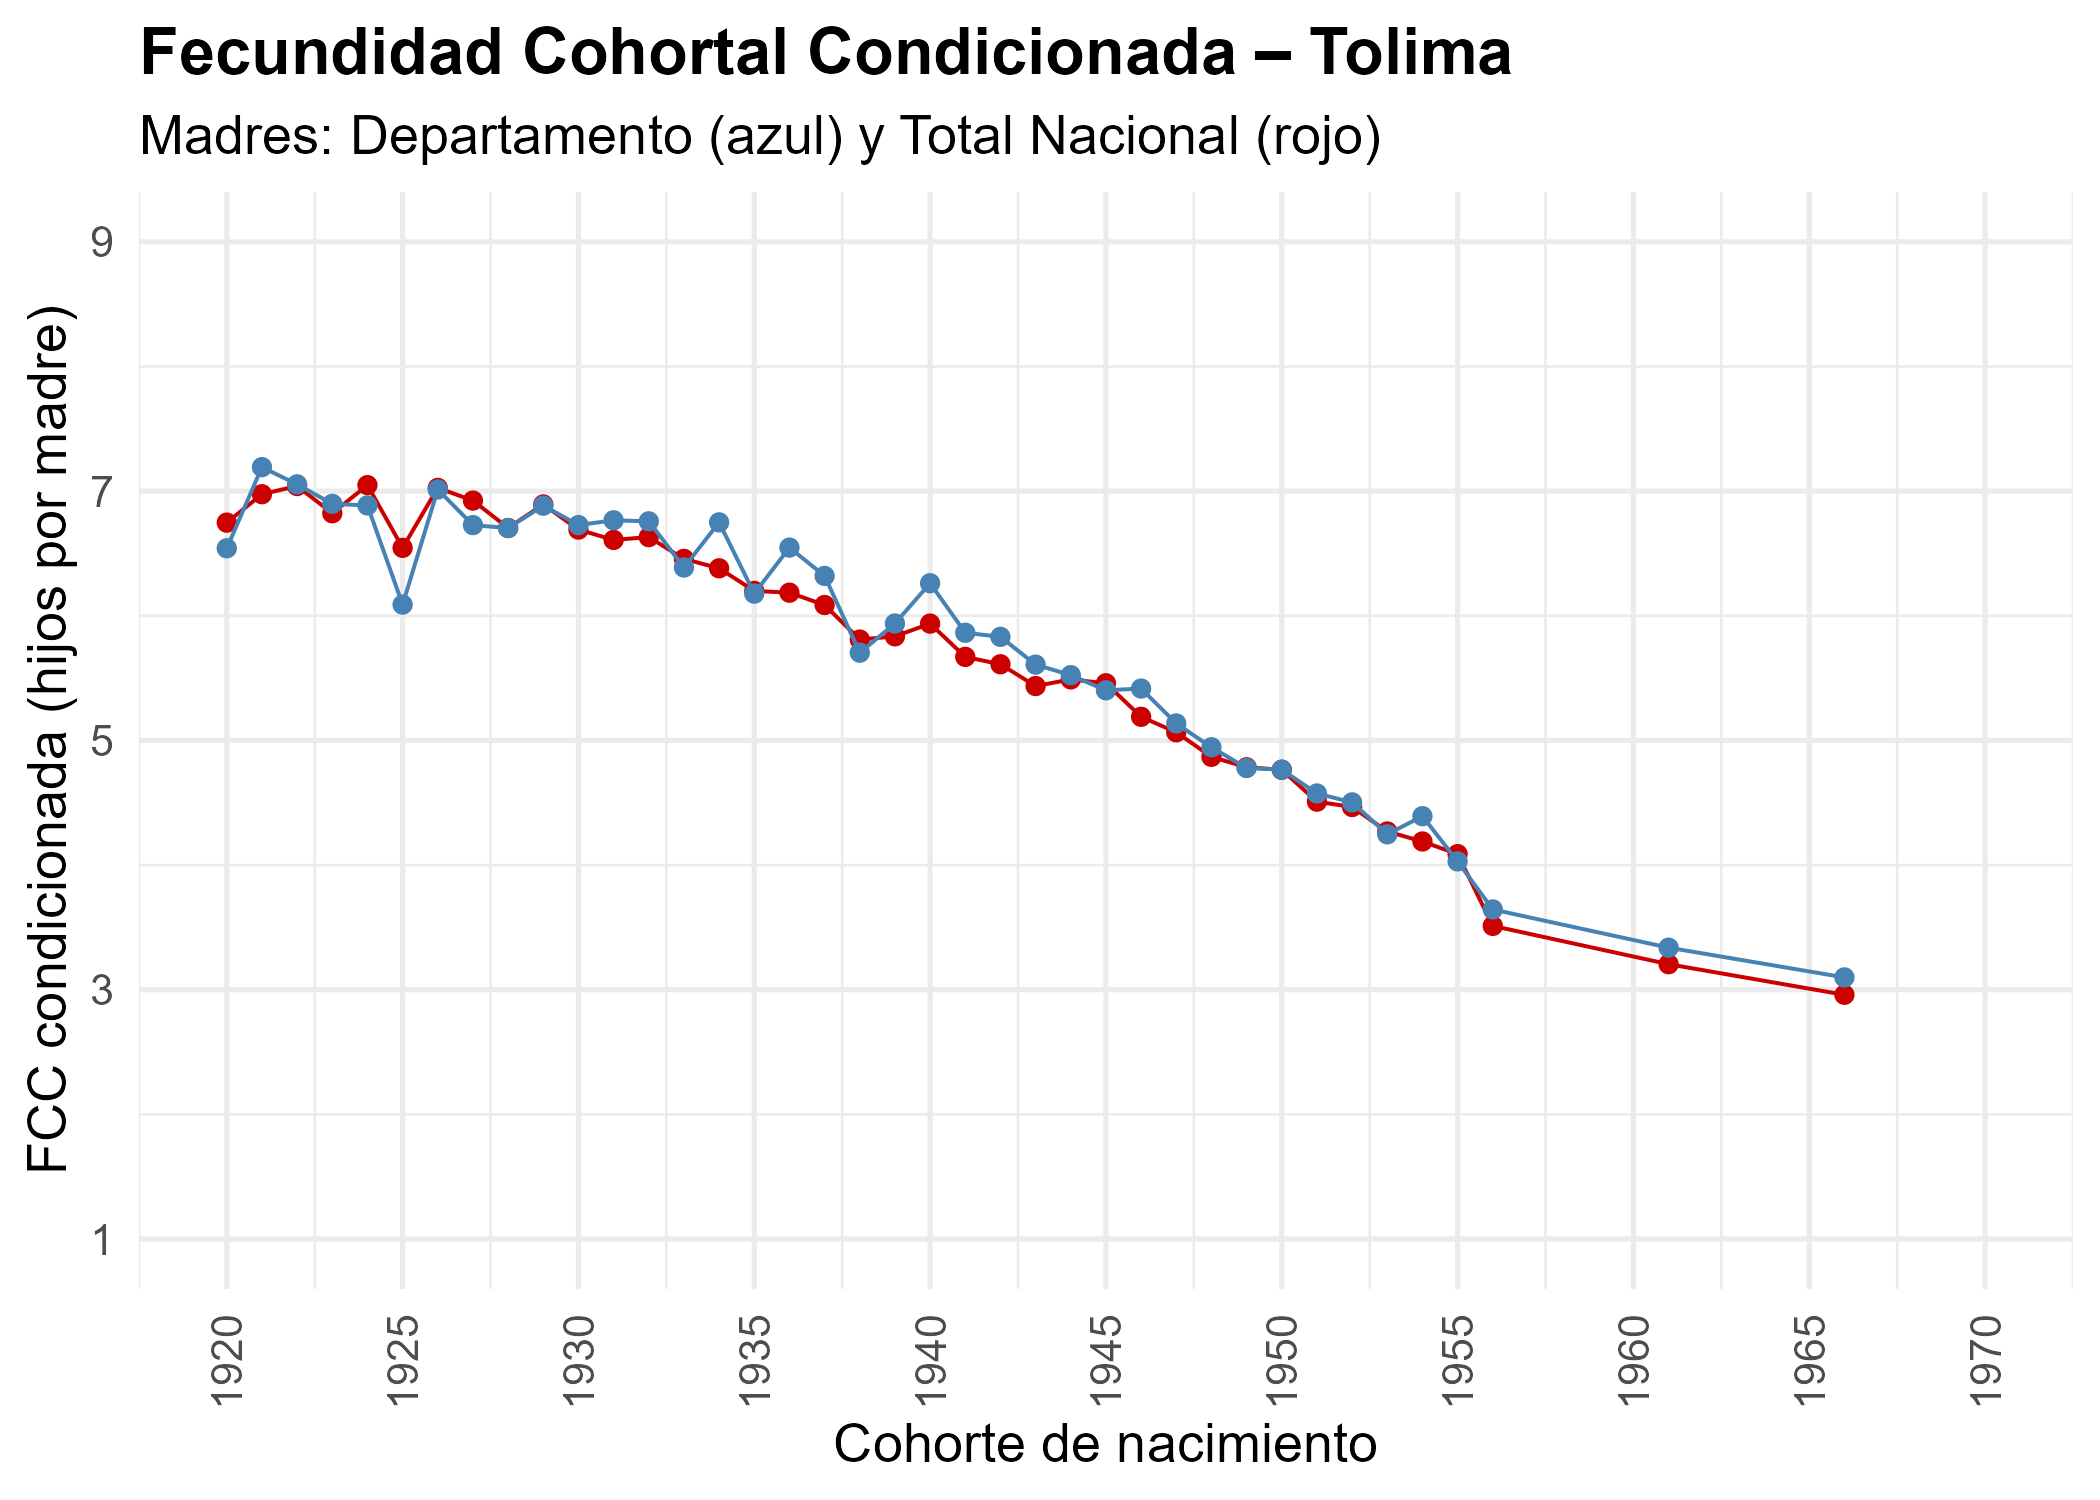
\includegraphics[width=\textwidth]{fcc_departamental/FCC_cond_Tolima_vs_National.png}
\end{columns}
\end{frame}
\begin{frame}{FCC: Valle del Cauca}
\begin{columns}
\column{0.5\textwidth}\centering
{\small Todas las mujeres}\\
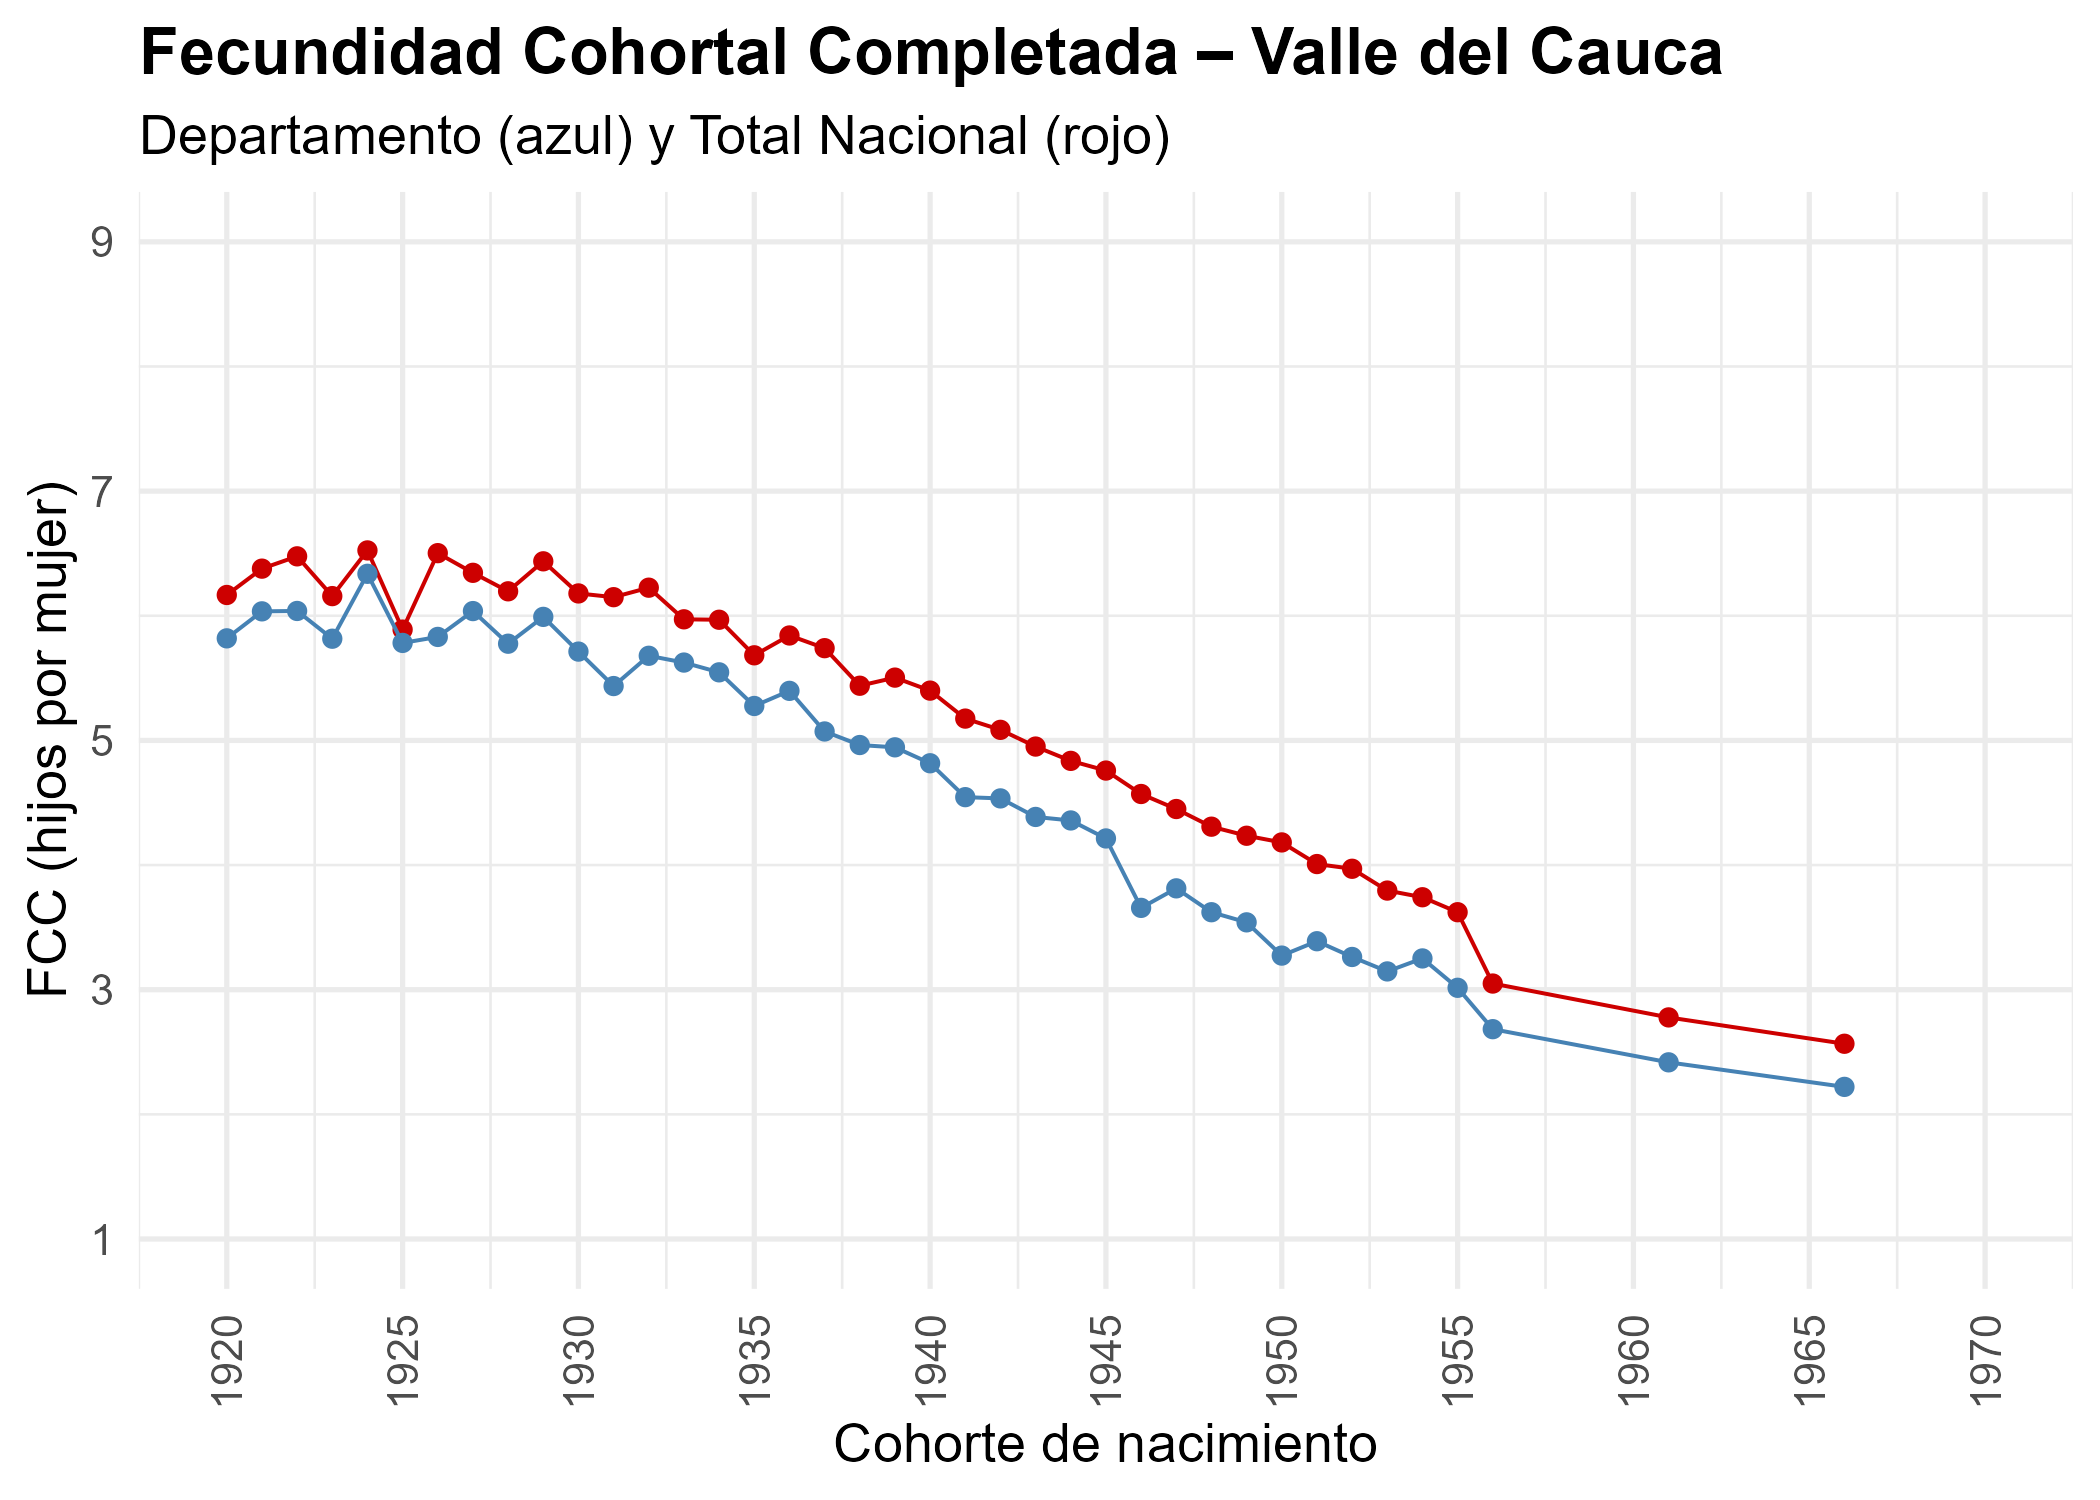
\includegraphics[width=\textwidth]{fcc_departamental/FCC_Valle del Cauca_vs_National.png}
\column{0.5\textwidth}\centering
{\small Condicional (madres)}\\
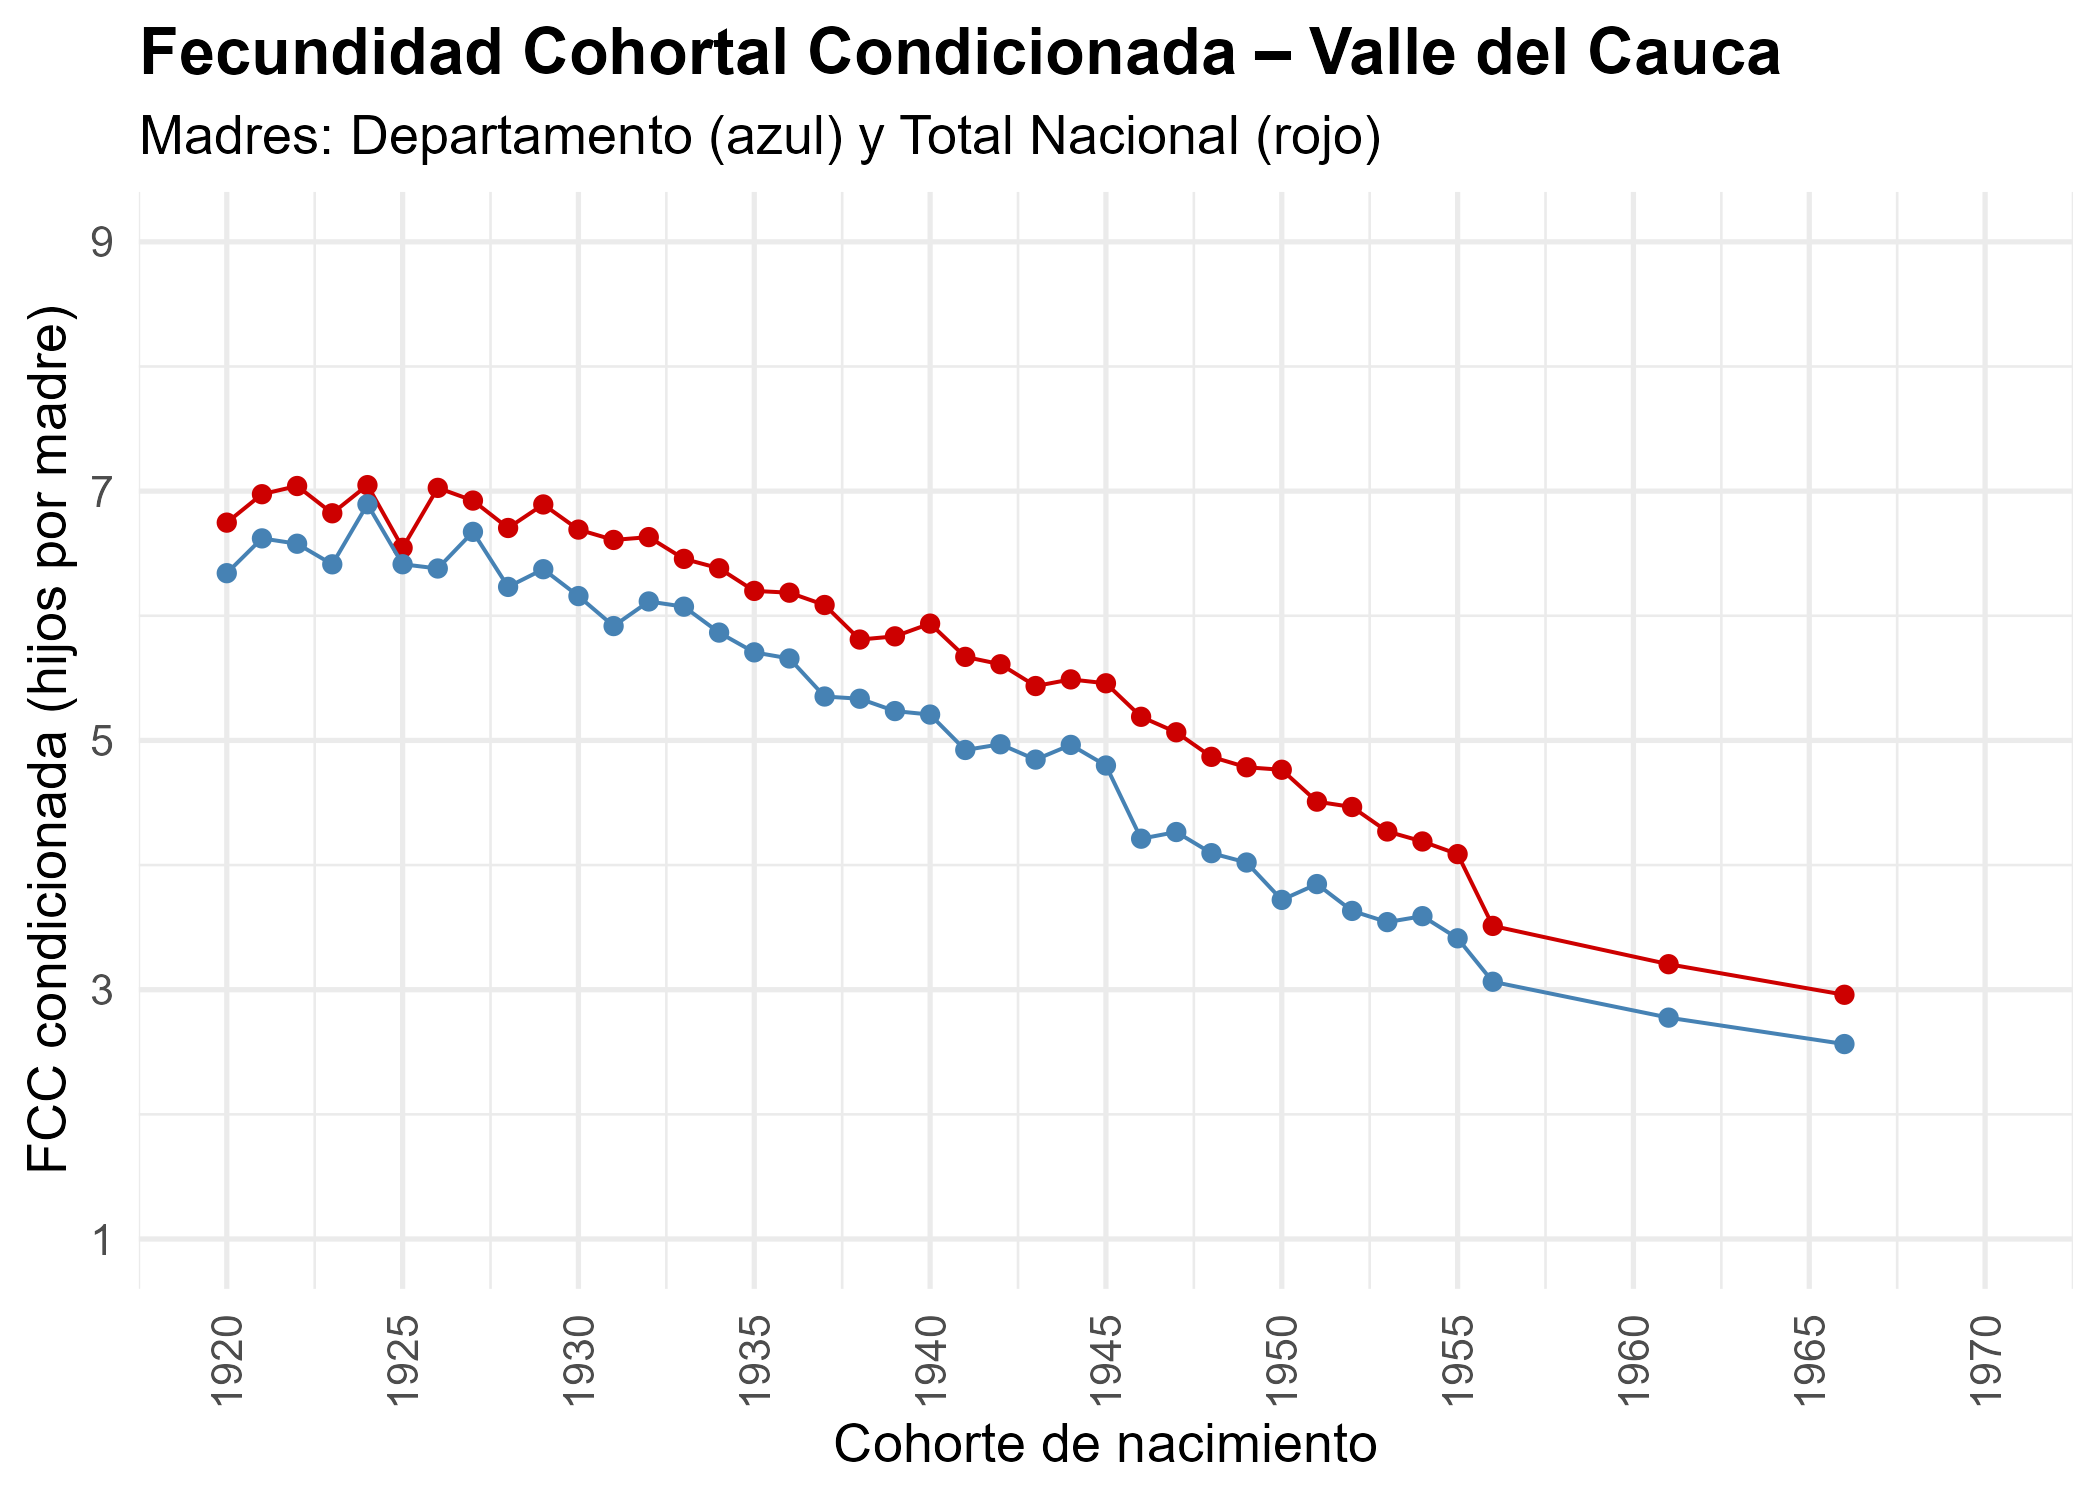
\includegraphics[width=\textwidth]{fcc_departamental/FCC_cond_Valle del Cauca_vs_National.png}
\end{columns}
\end{frame}
\section{TGF vs.\ FCC: per\'iodo y cohorte juntos}

\begin{frame}{Dos lentes sobre la misma transici\'on}
Superponer la TGF (lente de \alert{per\'iodo}) y la FCC condicional
(lente de \alert{cohorte}) permite ver si lo que cae es el ritmo anual
o el tama\~no final de las familias, y detectar efectos de calendario.
Las siguientes 22 diapositivas lo muestran para cada departamento.
\end{frame}
\begin{frame}{TGF vs.\ FCC: Amazonas}
\begin{center}
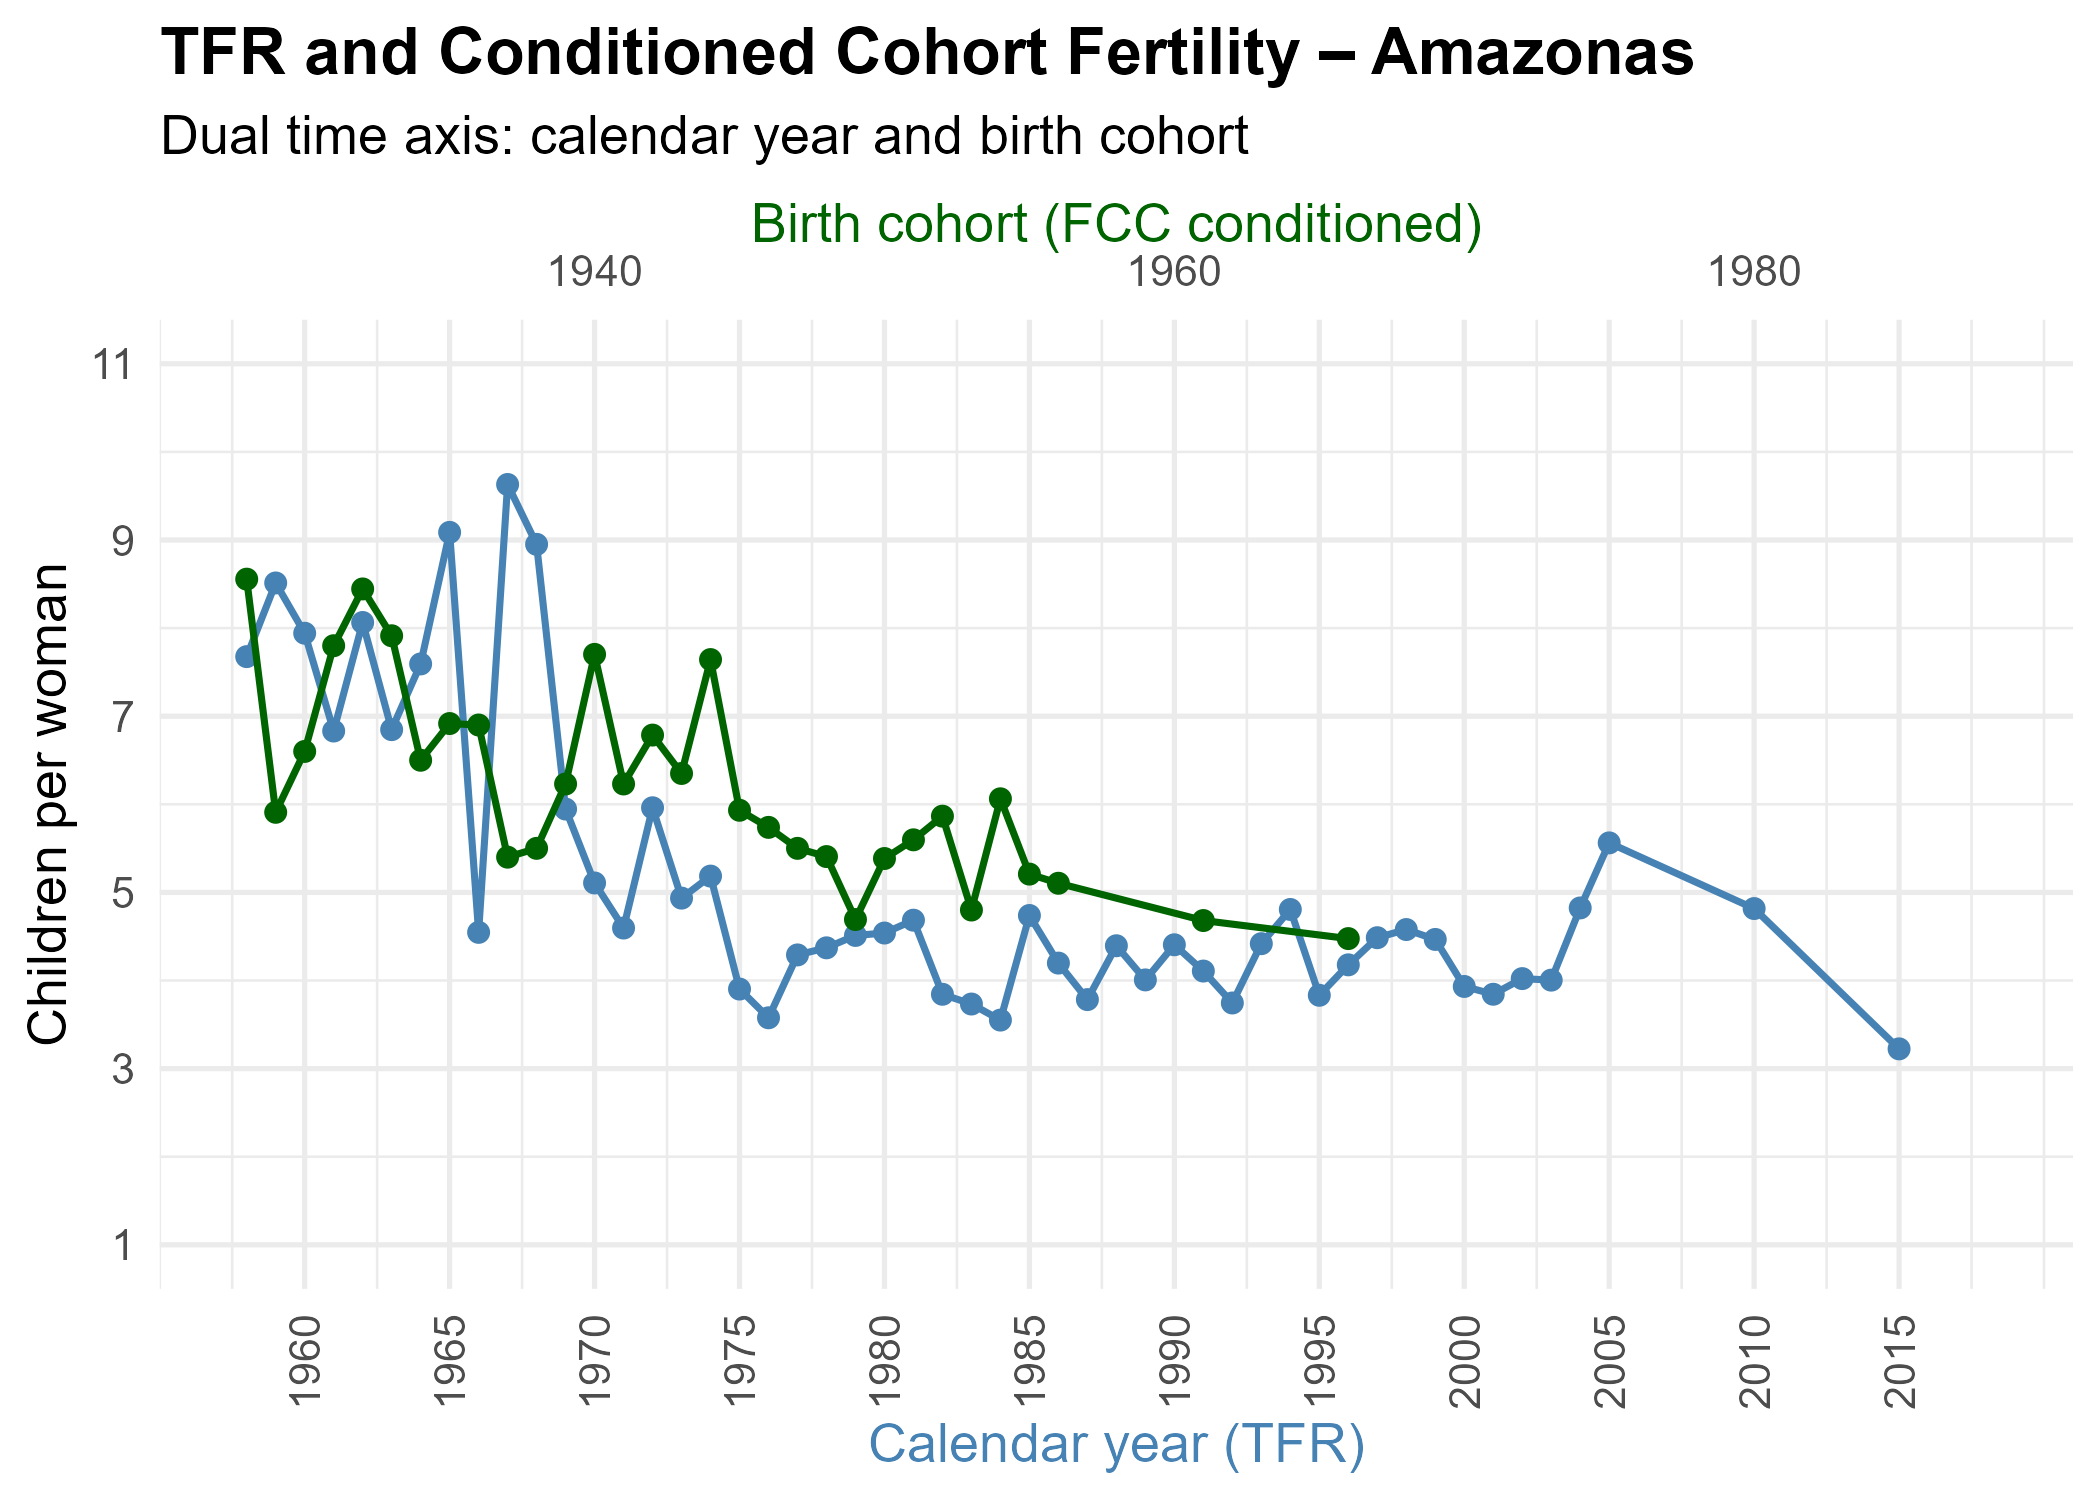
\includegraphics[height=0.78\textheight]{tfr_vs_fcc/TFR_FCCcond_Amazonas.png}
\end{center}
\end{frame}
\begin{frame}{TGF vs.\ FCC: Antioquia}
\begin{center}
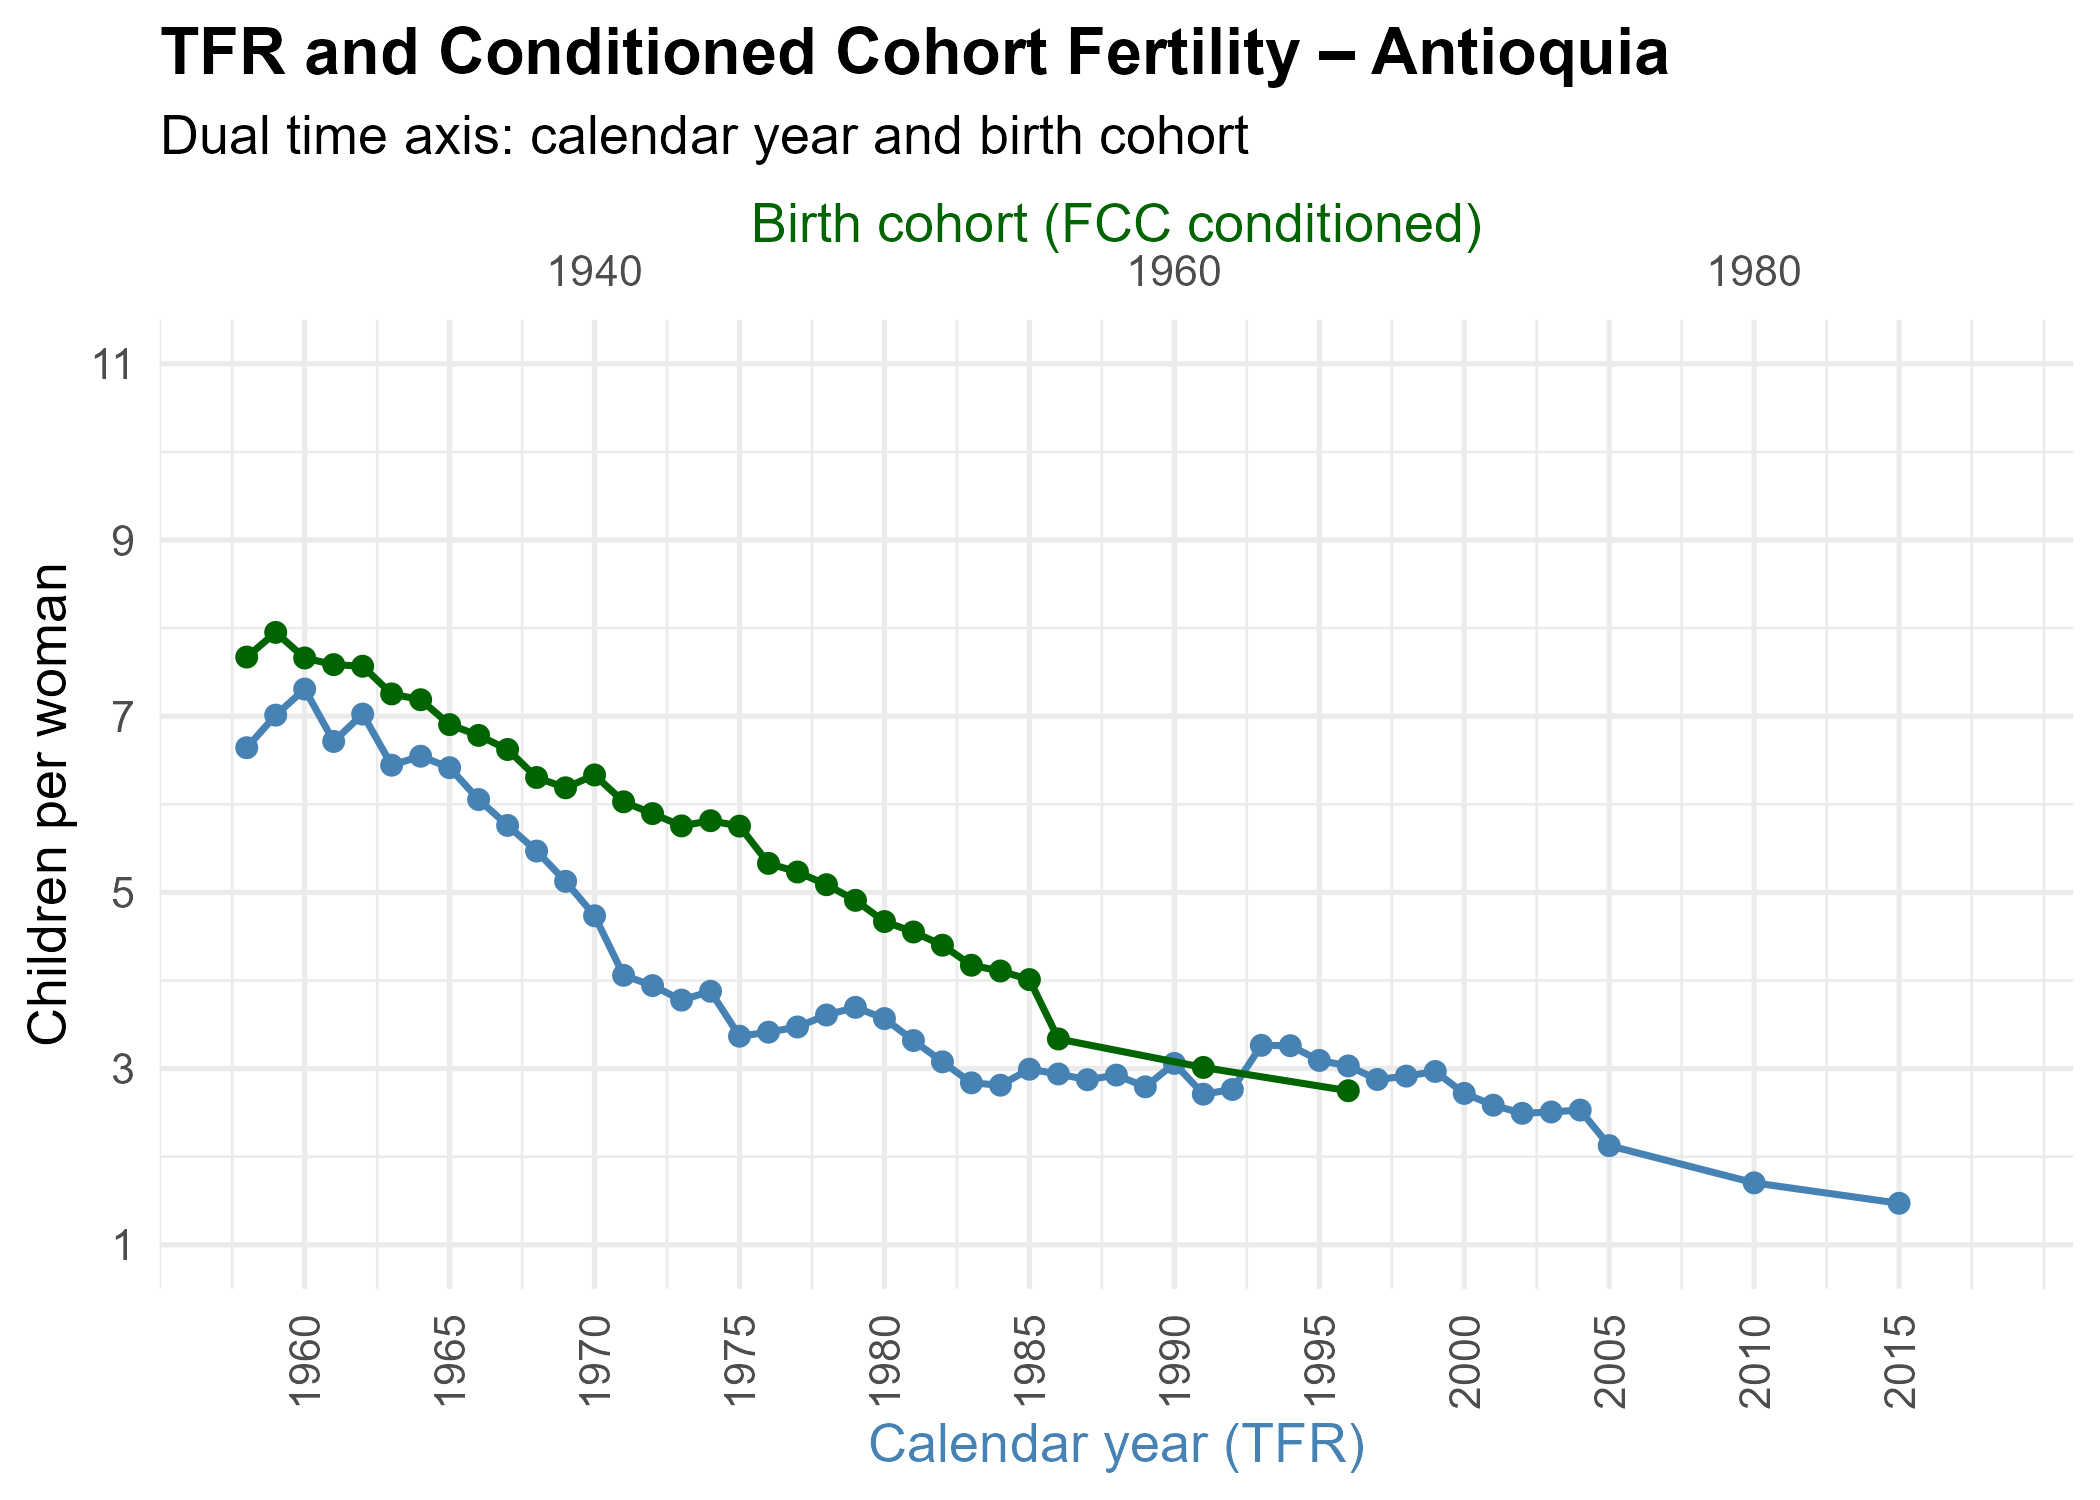
\includegraphics[height=0.78\textheight]{tfr_vs_fcc/TFR_FCCcond_Antioquia.png}
\end{center}
\end{frame}
\begin{frame}{TGF vs.\ FCC: Arauca}
\begin{center}
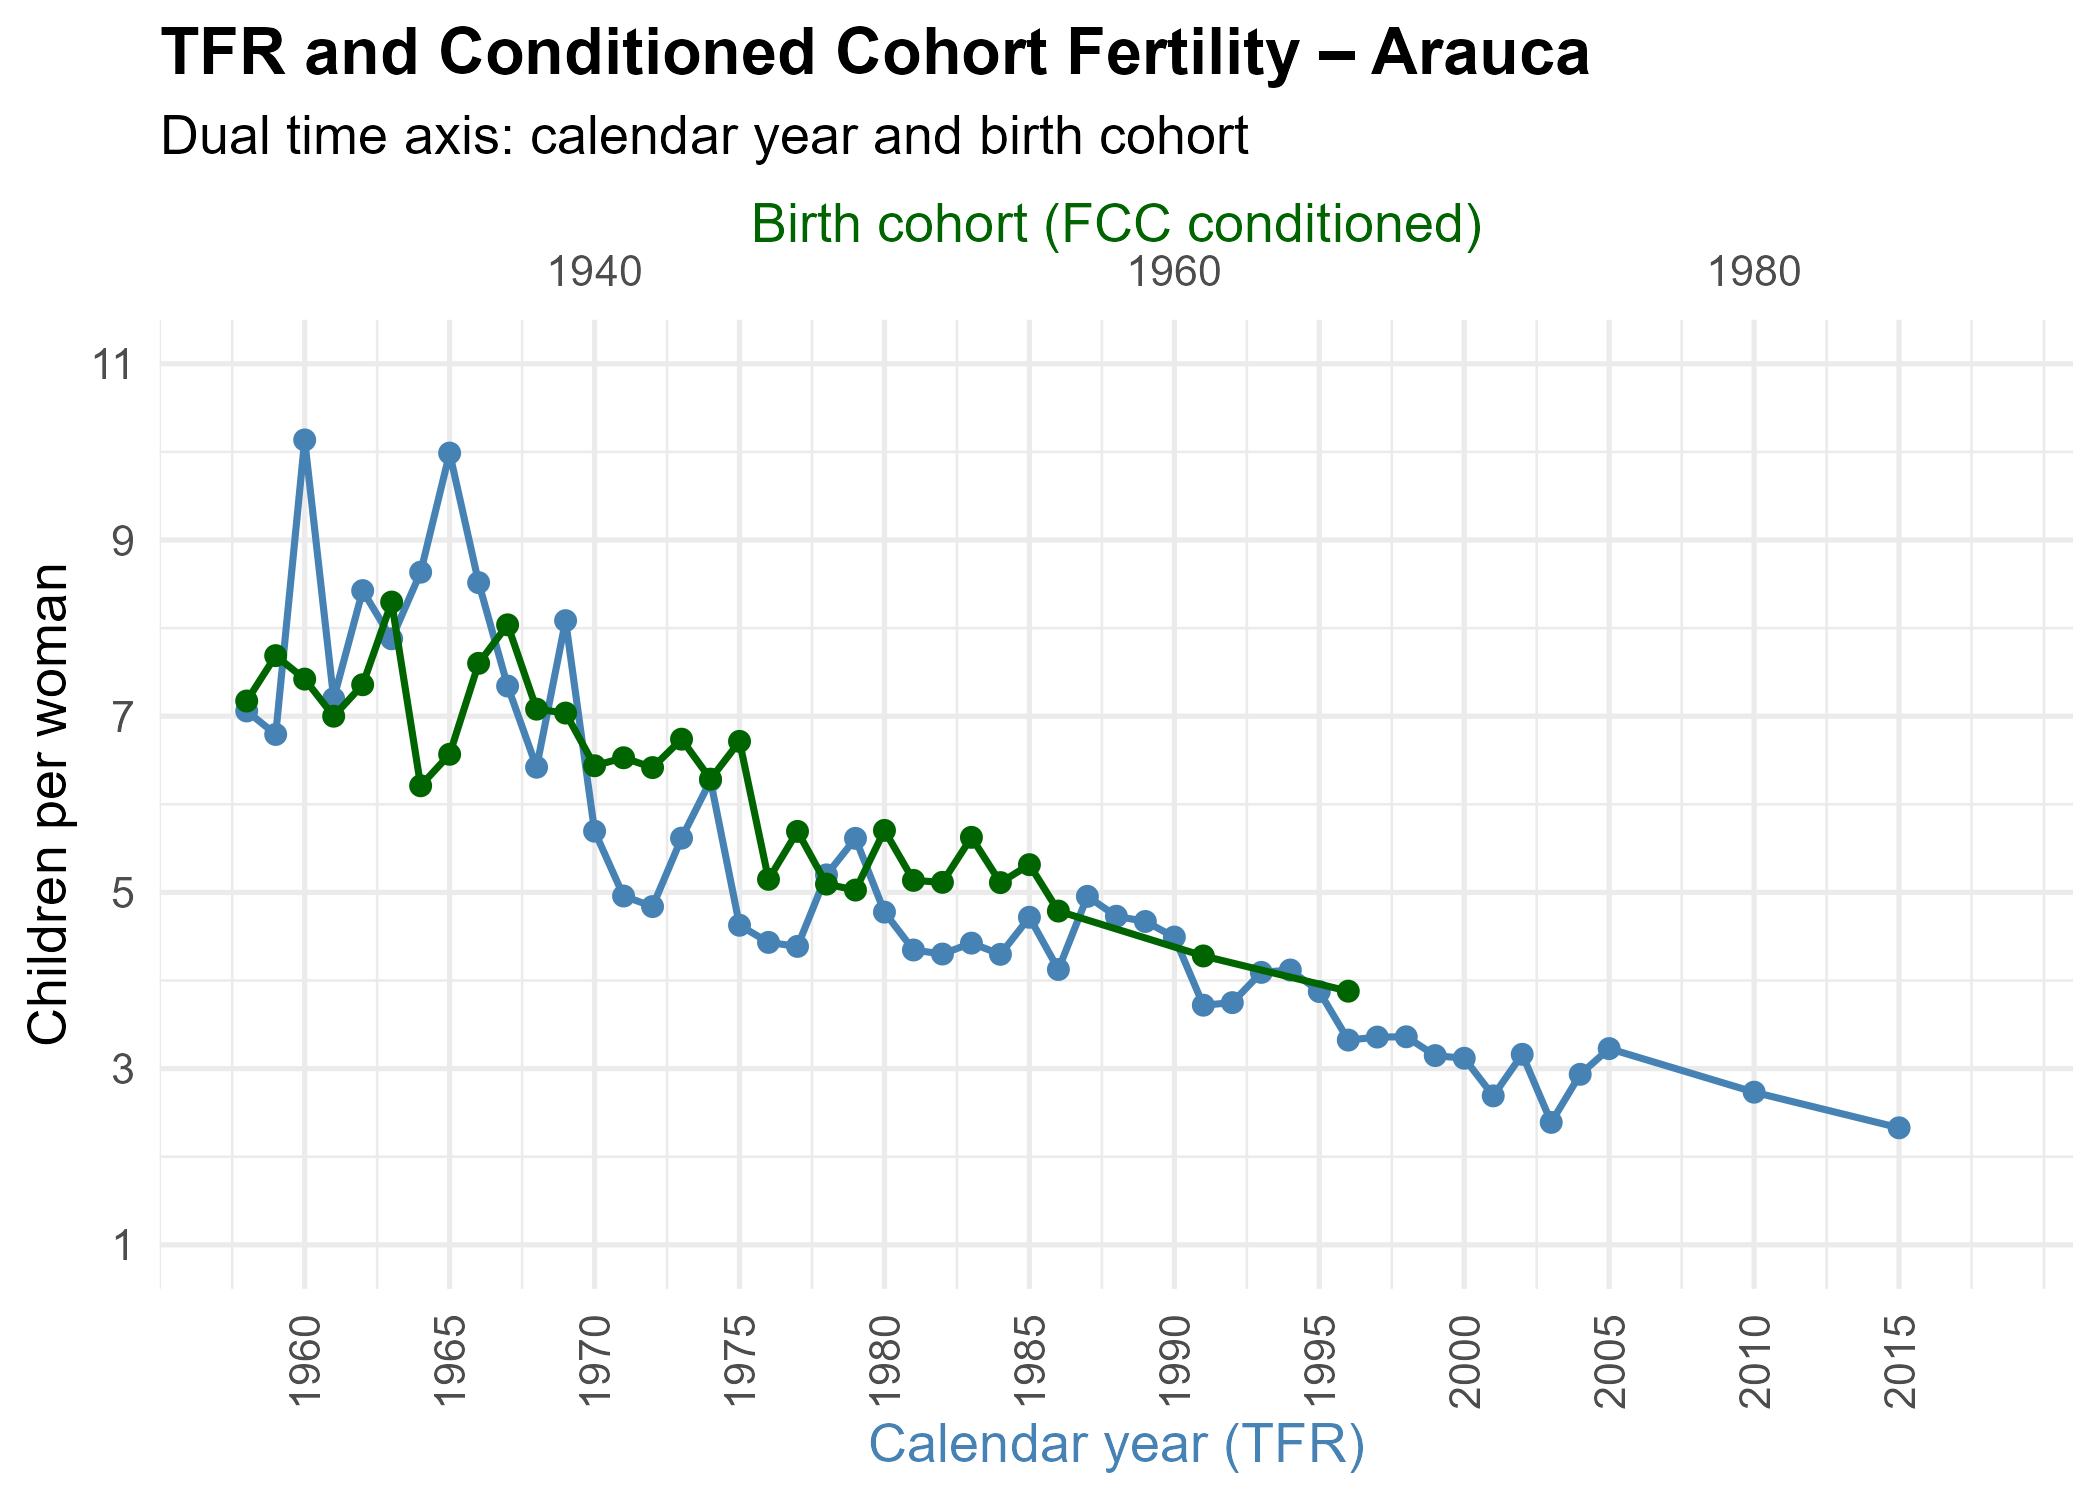
\includegraphics[height=0.78\textheight]{tfr_vs_fcc/TFR_FCCcond_Arauca.png}
\end{center}
\end{frame}
\begin{frame}{TGF vs.\ FCC: Atlántico}
\begin{center}
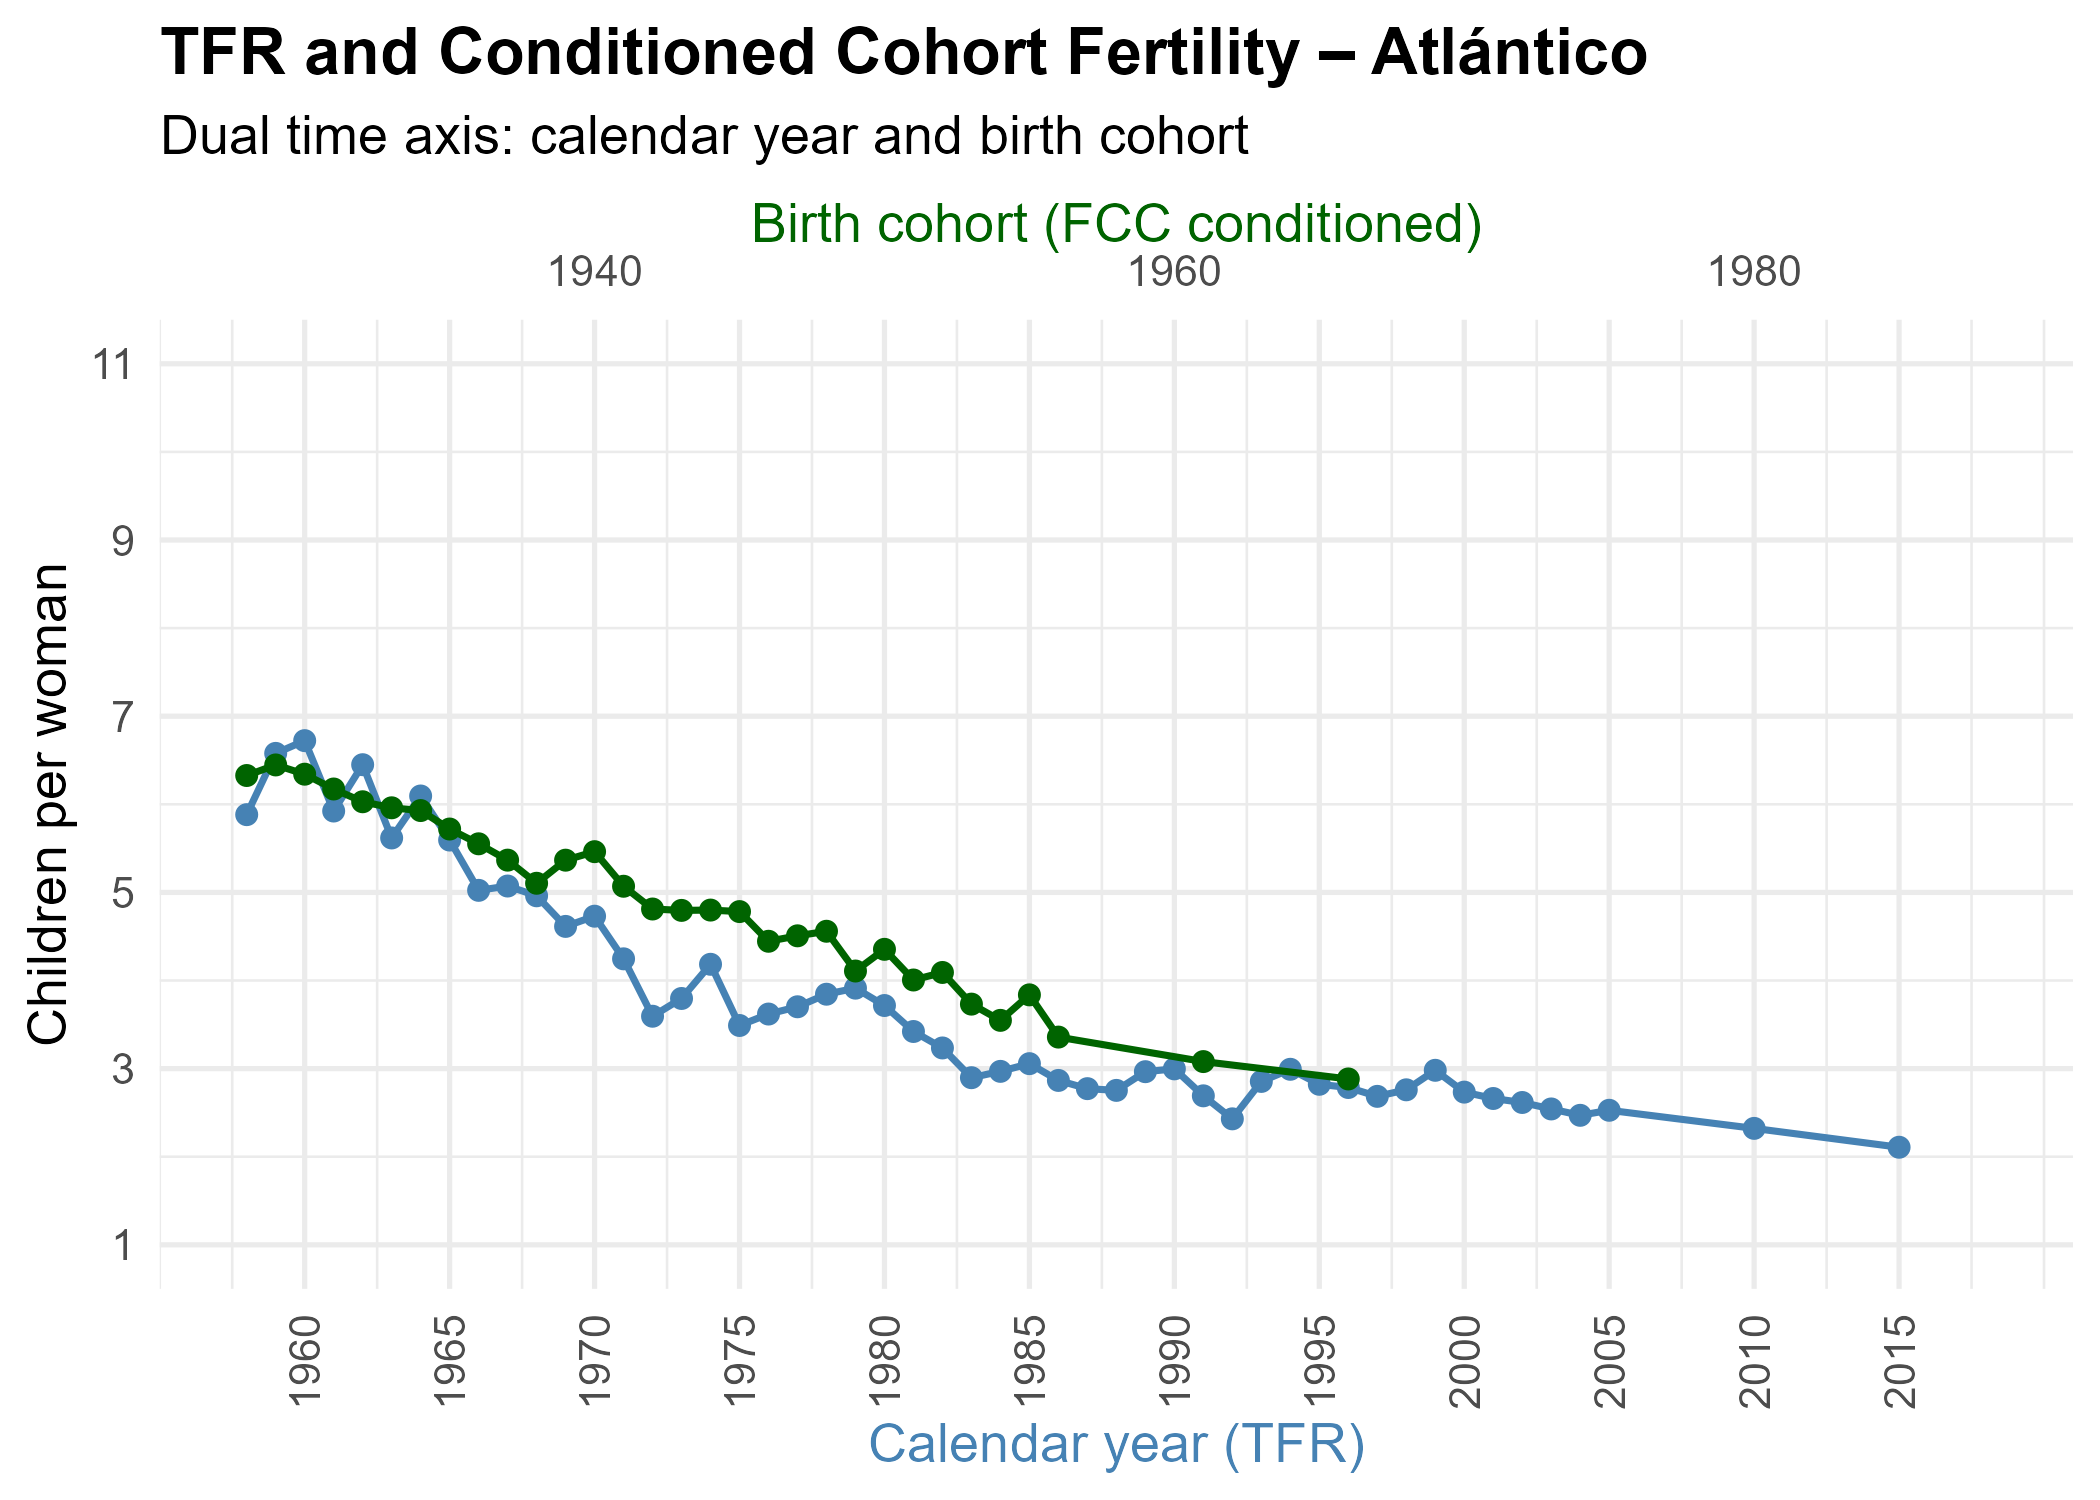
\includegraphics[height=0.78\textheight]{tfr_vs_fcc/TFR_FCCcond_Atlántico.png}
\end{center}
\end{frame}
\begin{frame}{TGF vs.\ FCC: Bogotá D.C.}
\begin{center}
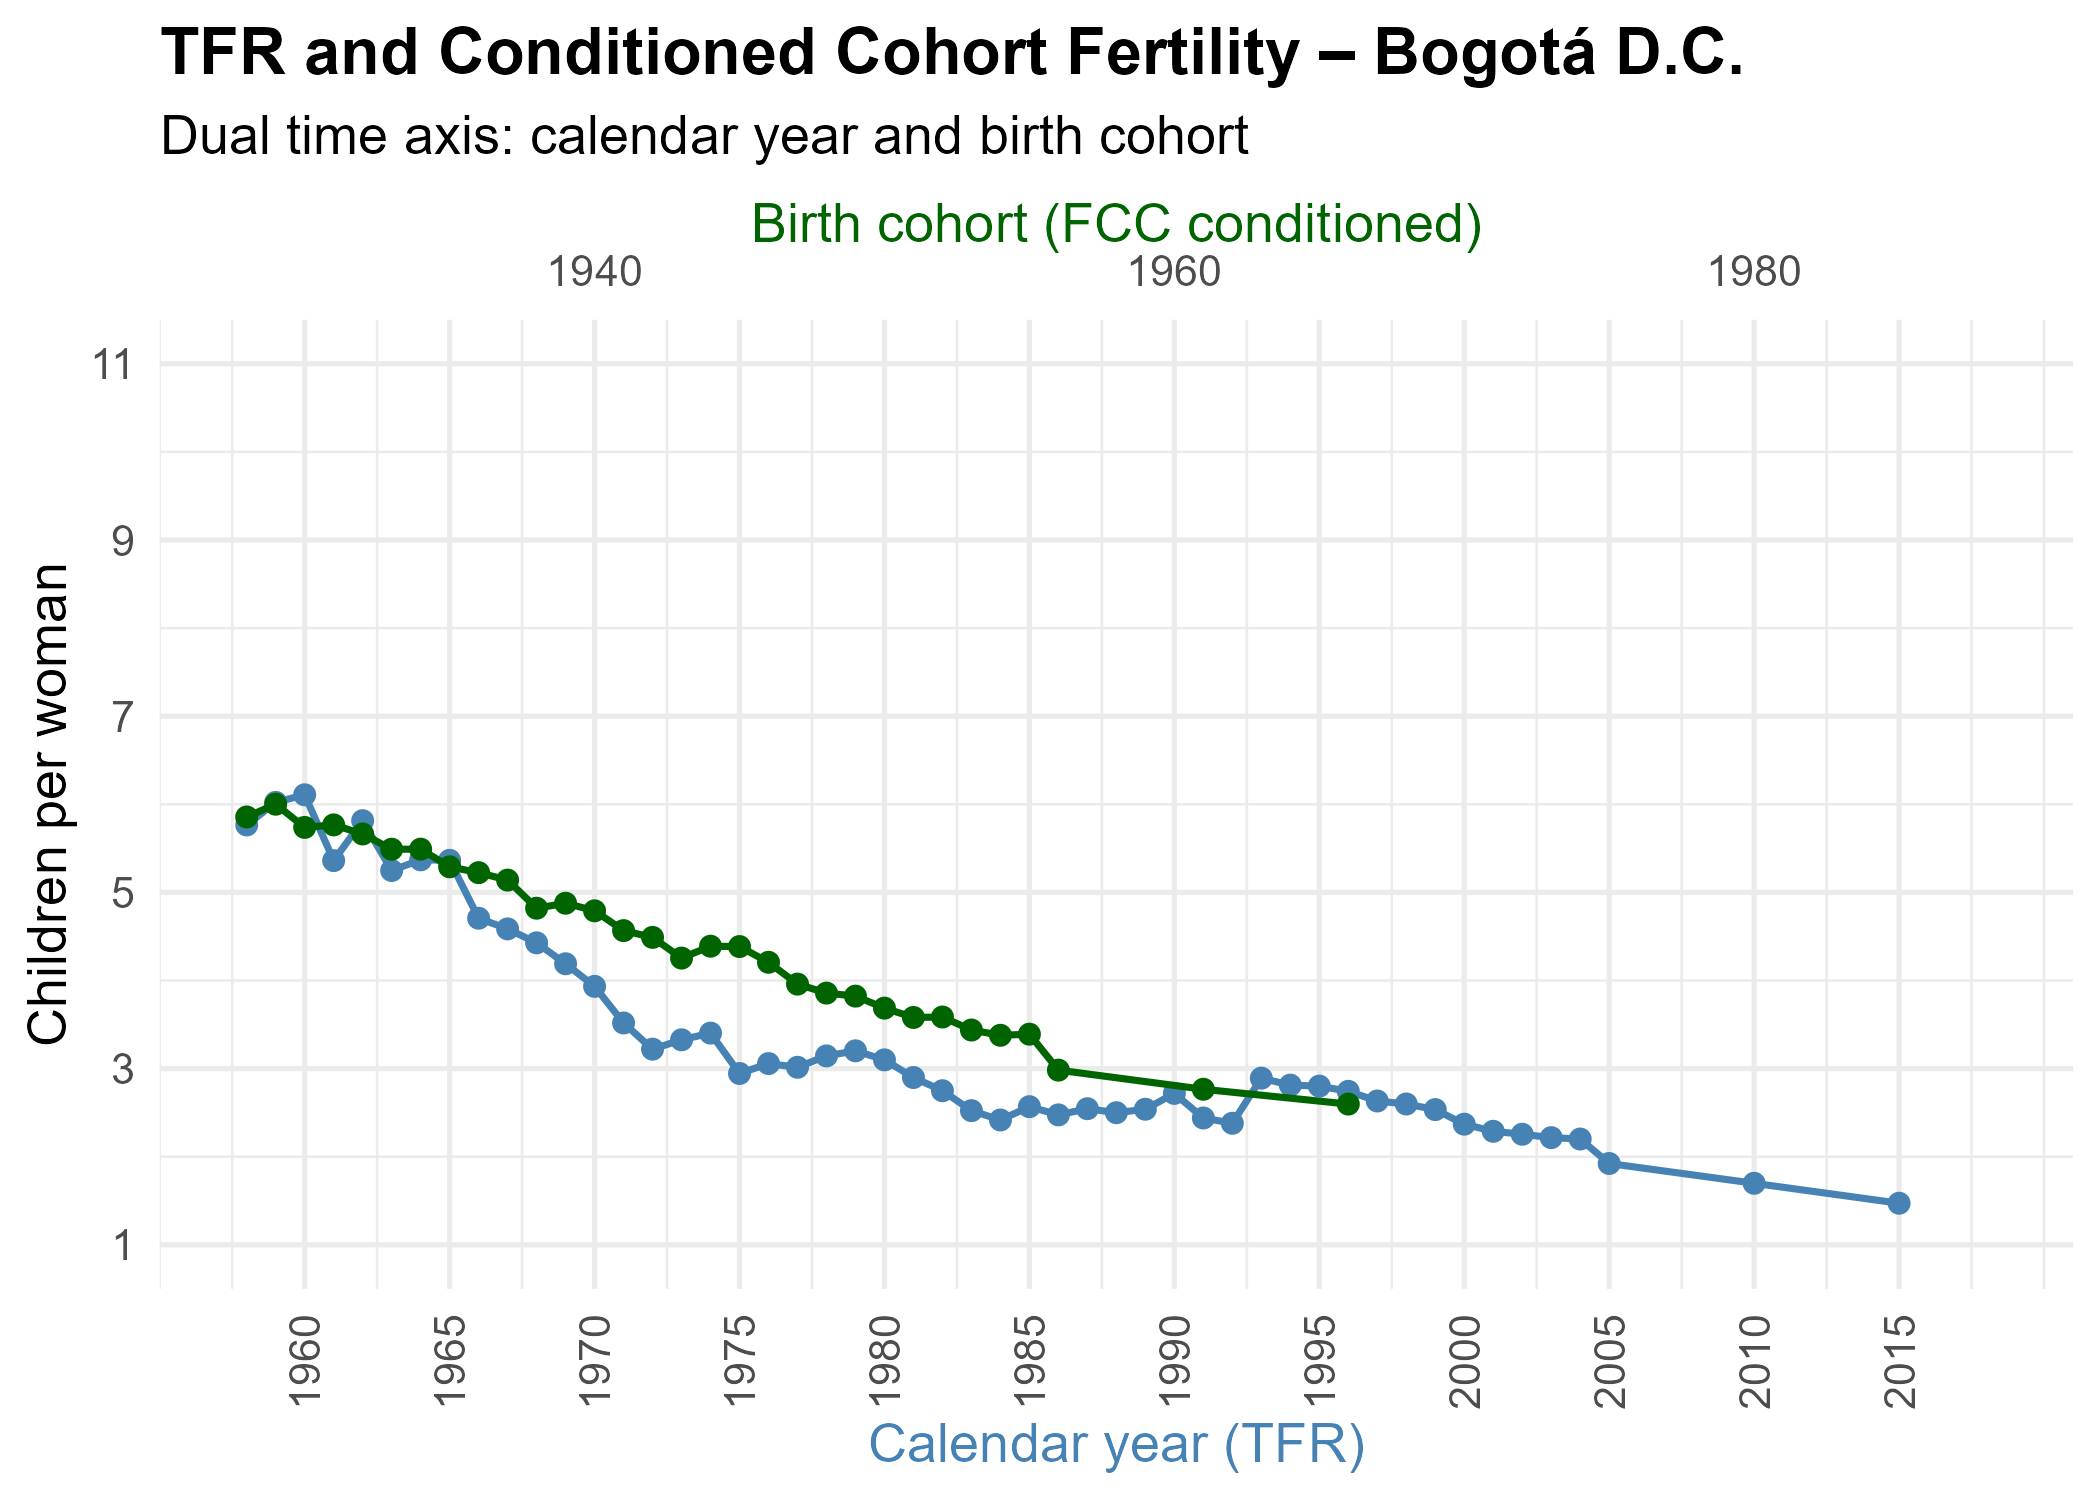
\includegraphics[height=0.78\textheight]{tfr_vs_fcc/TFR_FCCcond_Bogotá D.C..png}
\end{center}
\end{frame}
\begin{frame}{TGF vs.\ FCC: Bolívar}
\begin{center}
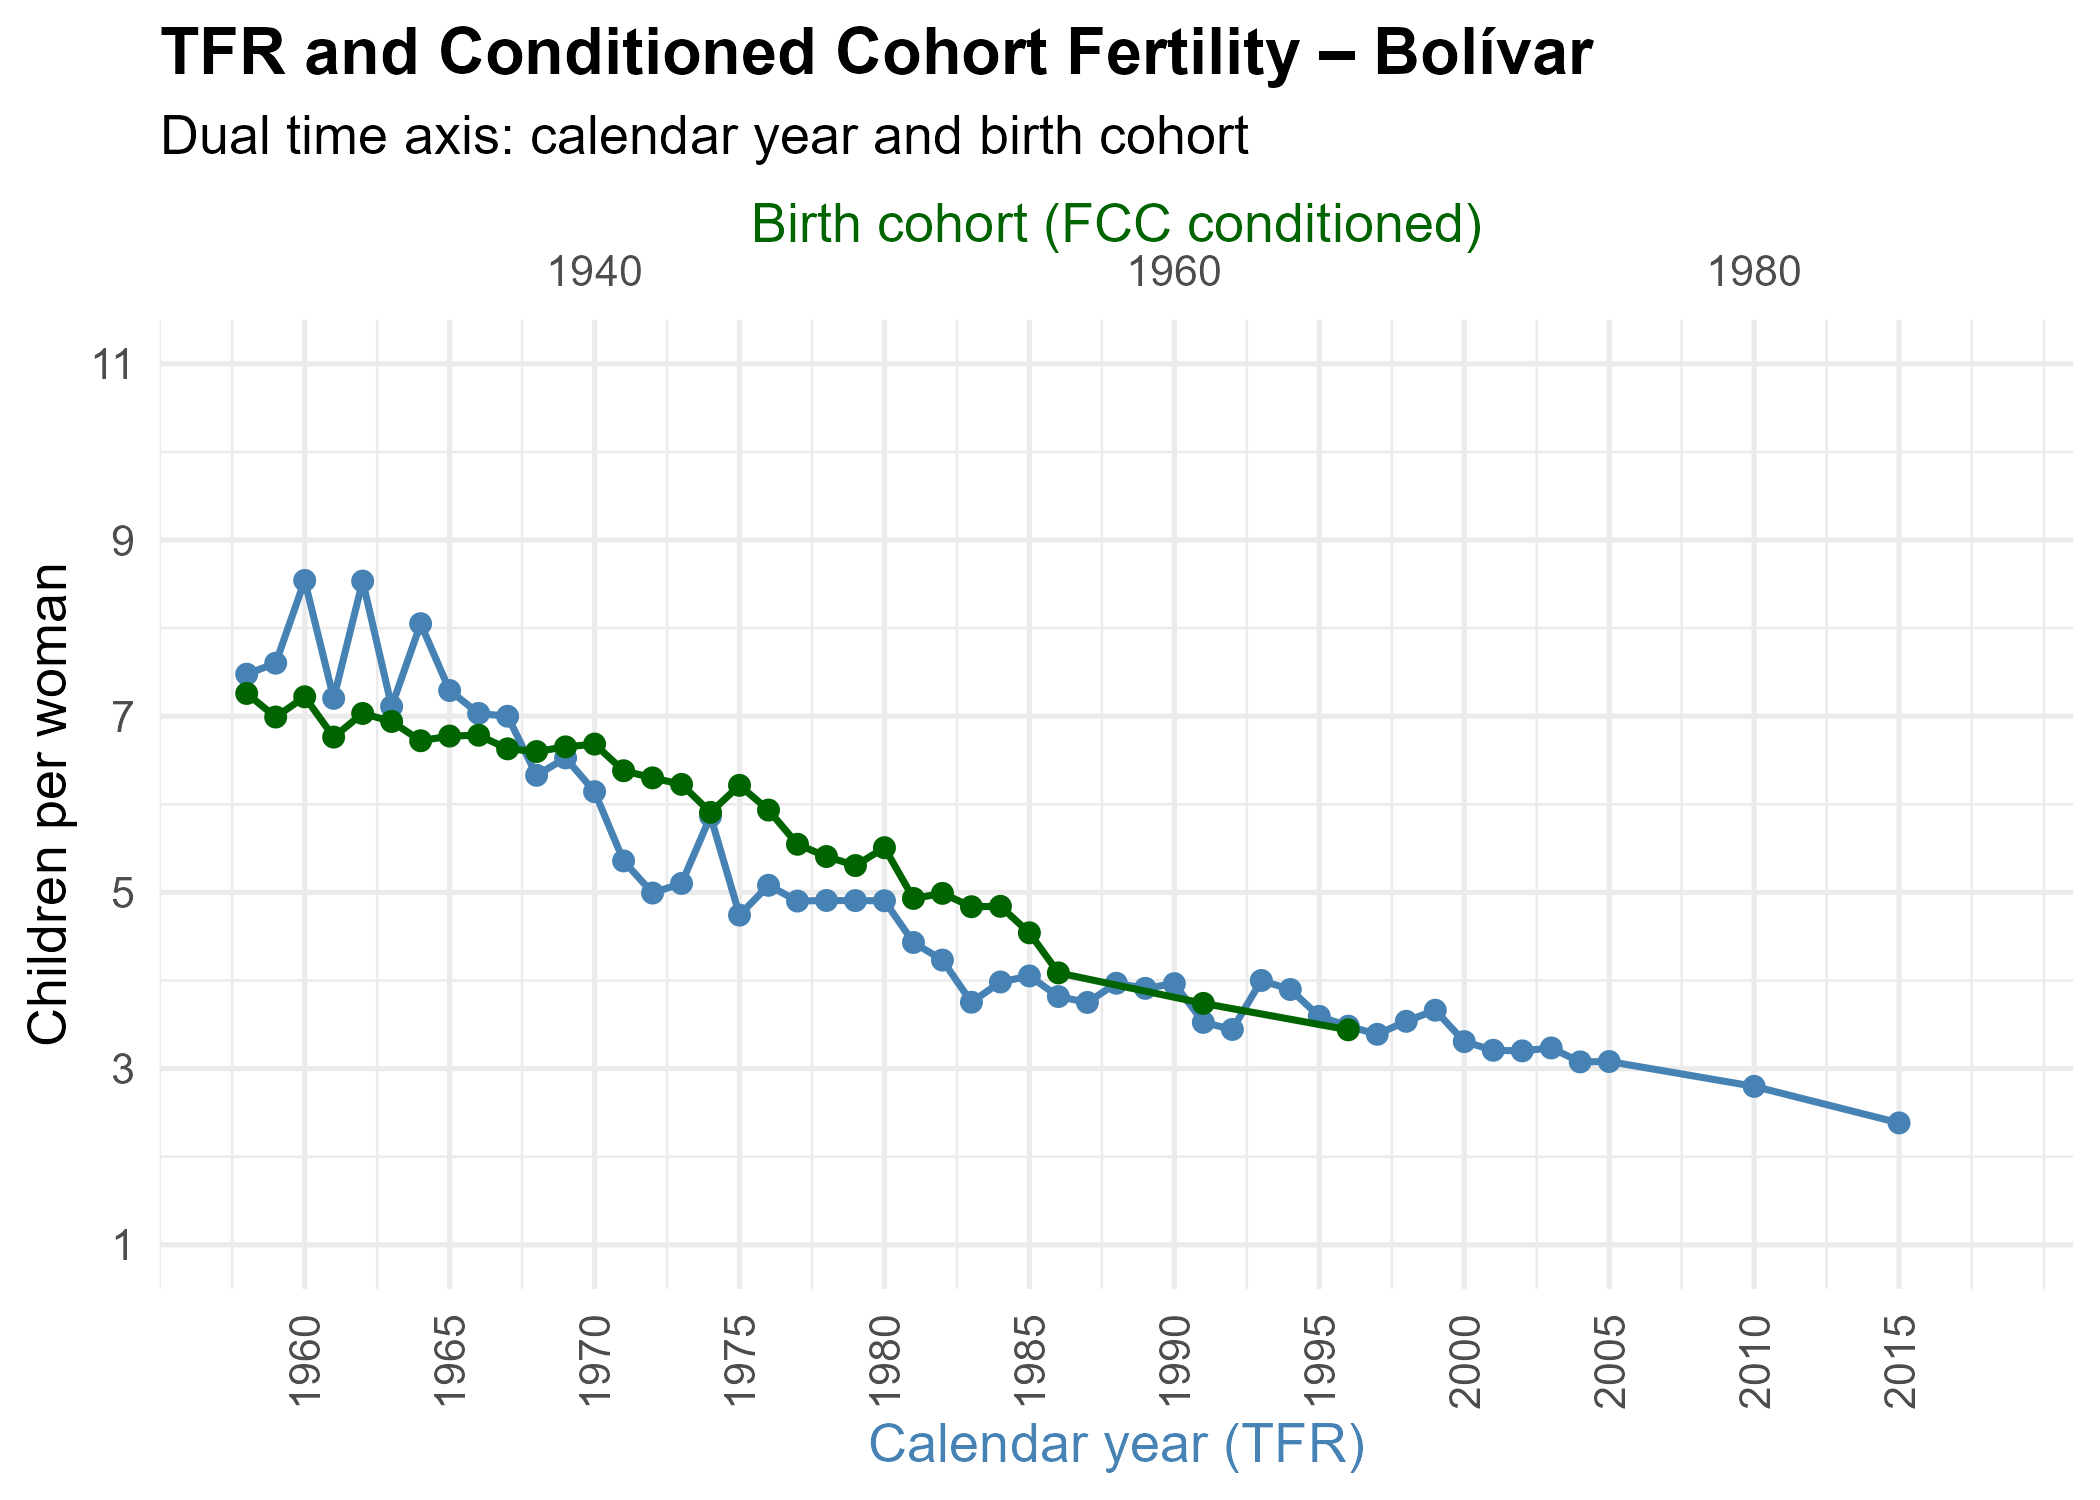
\includegraphics[height=0.78\textheight]{tfr_vs_fcc/TFR_FCCcond_Bolívar.png}
\end{center}
\end{frame}
\begin{frame}{TGF vs.\ FCC: Boyacá}
\begin{center}
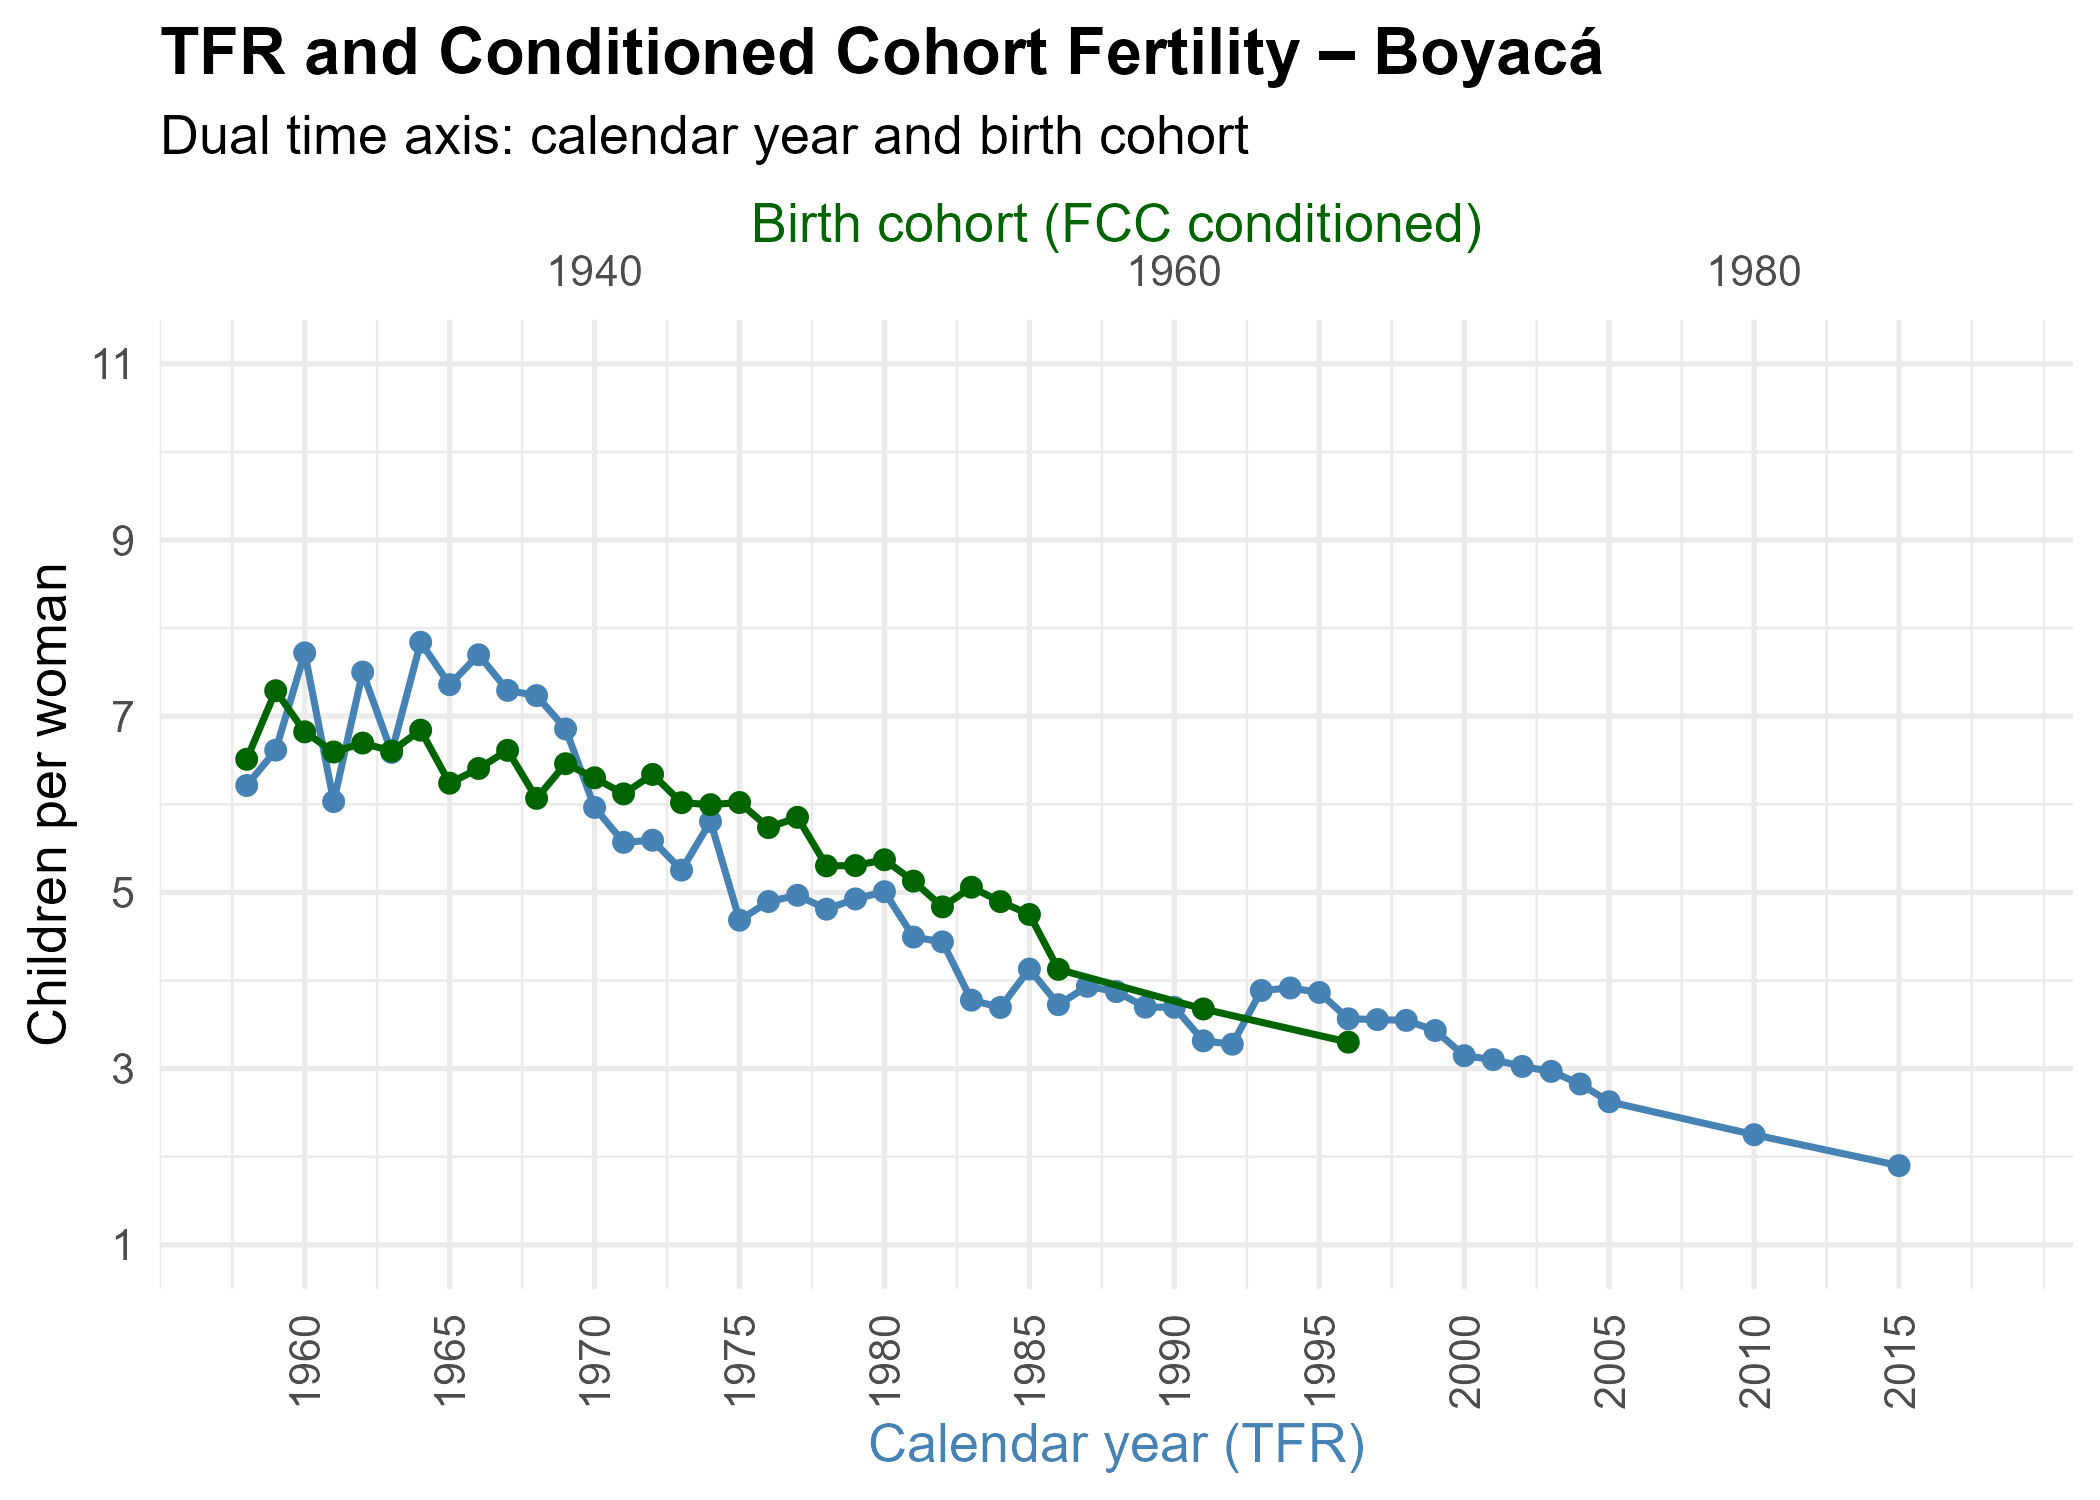
\includegraphics[height=0.78\textheight]{tfr_vs_fcc/TFR_FCCcond_Boyacá.png}
\end{center}
\end{frame}
\begin{frame}{TGF vs.\ FCC: Caldas}
\begin{center}
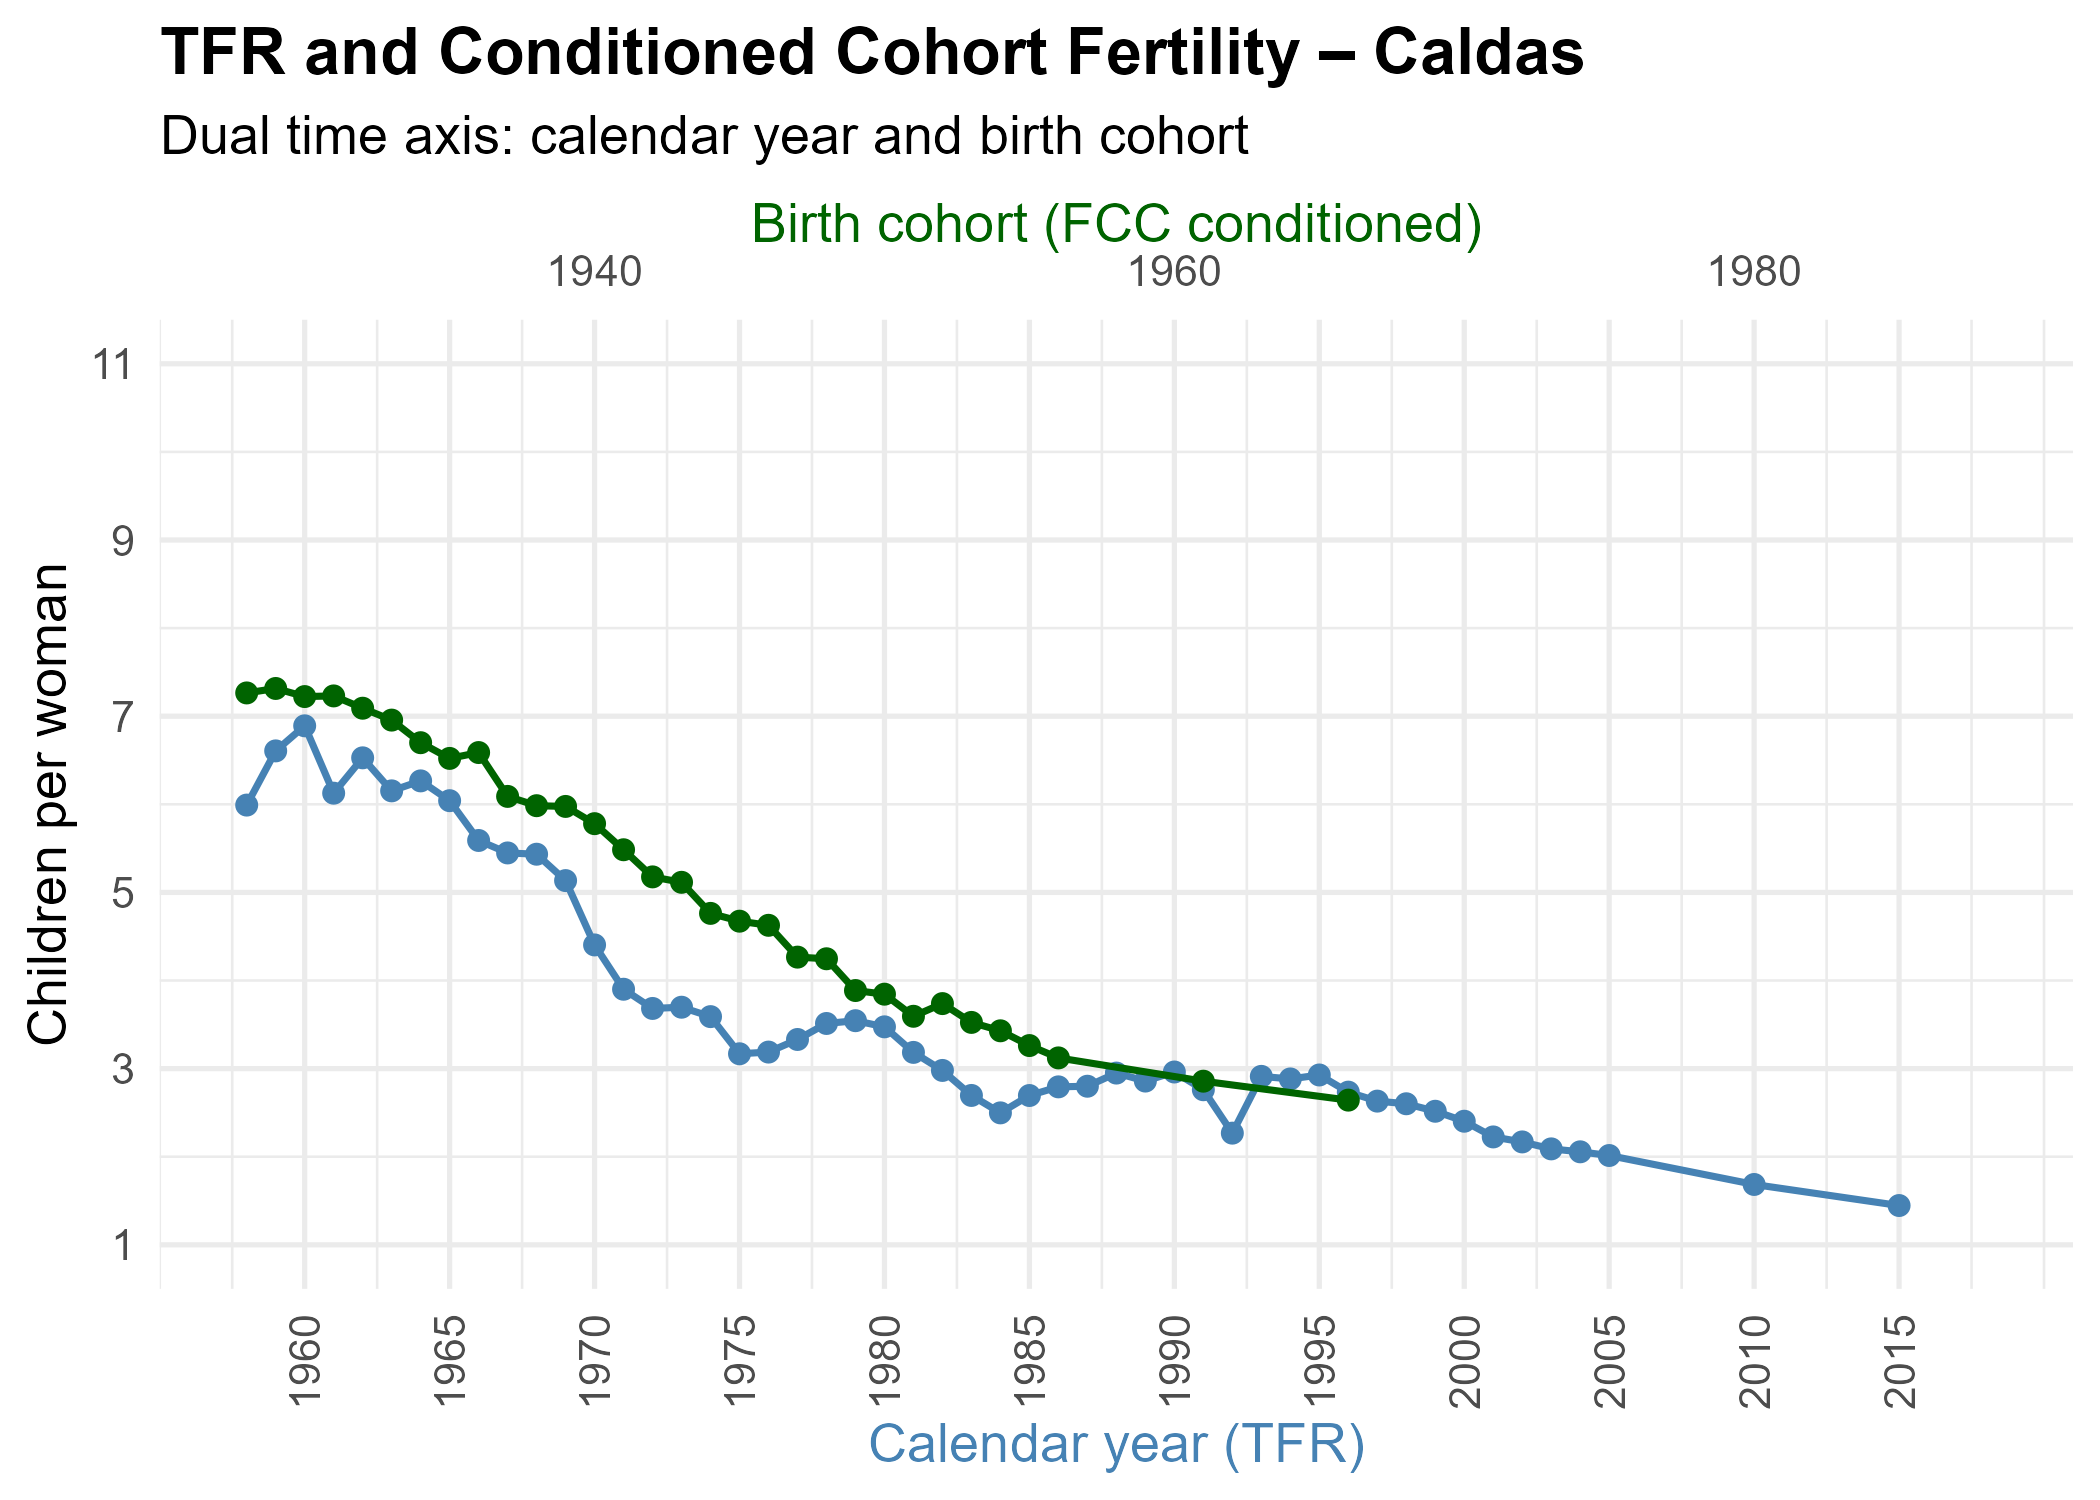
\includegraphics[height=0.78\textheight]{tfr_vs_fcc/TFR_FCCcond_Caldas.png}
\end{center}
\end{frame}
\begin{frame}{TGF vs.\ FCC: Caquetá}
\begin{center}
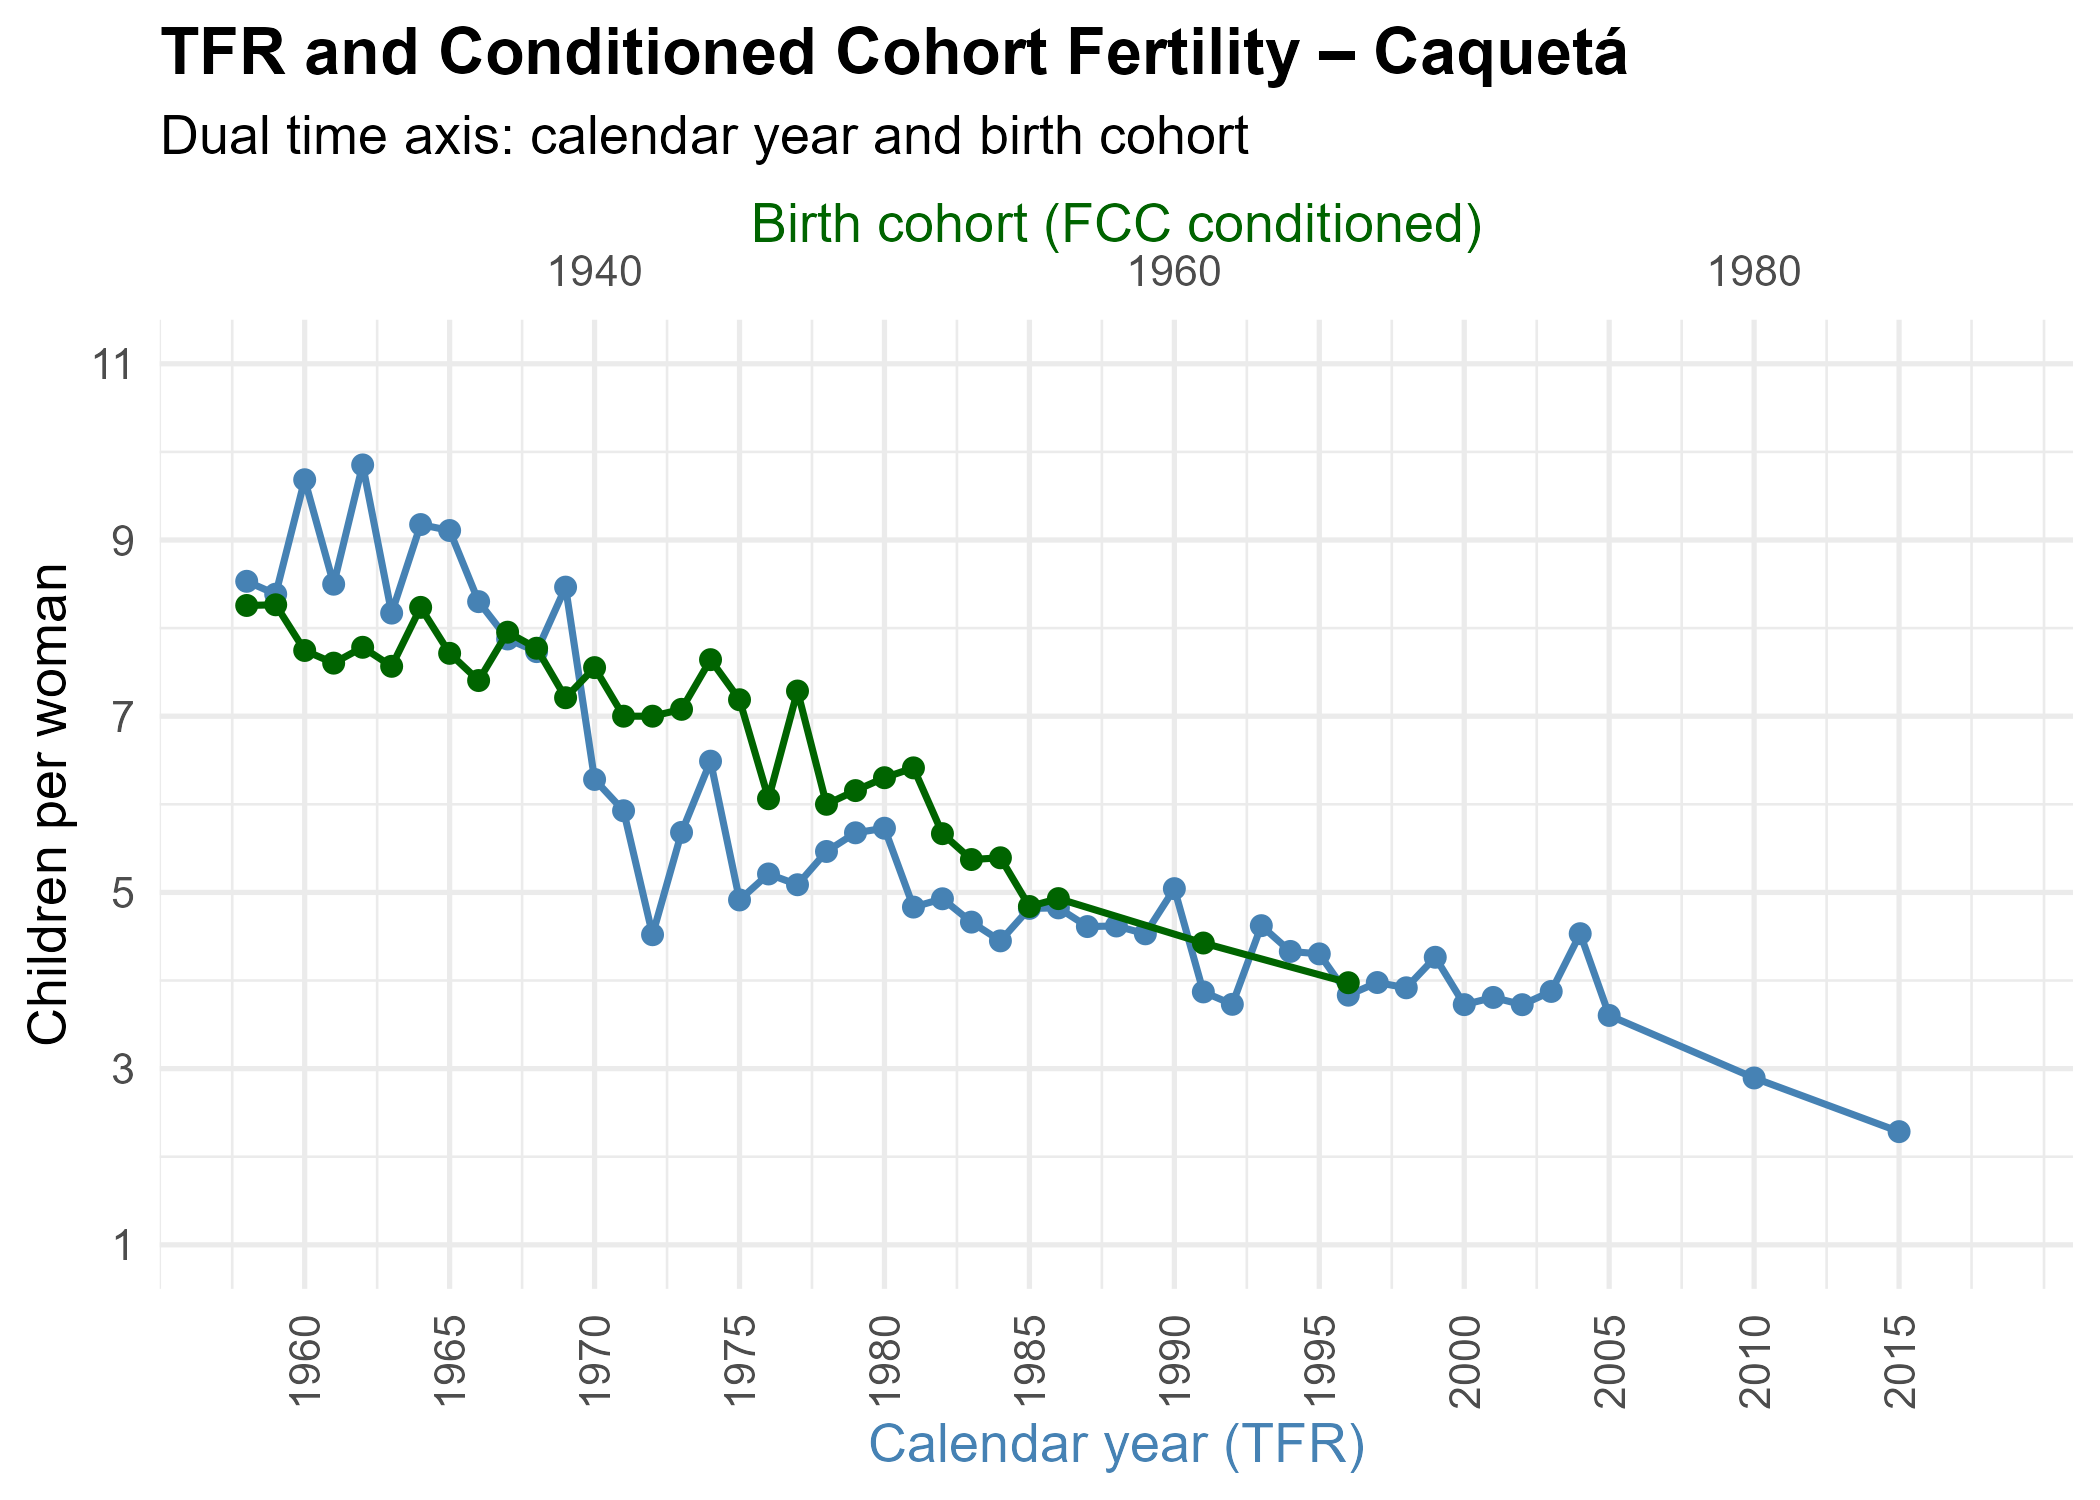
\includegraphics[height=0.78\textheight]{tfr_vs_fcc/TFR_FCCcond_Caquetá.png}
\end{center}
\end{frame}
\begin{frame}{TGF vs.\ FCC: Cauca}
\begin{center}
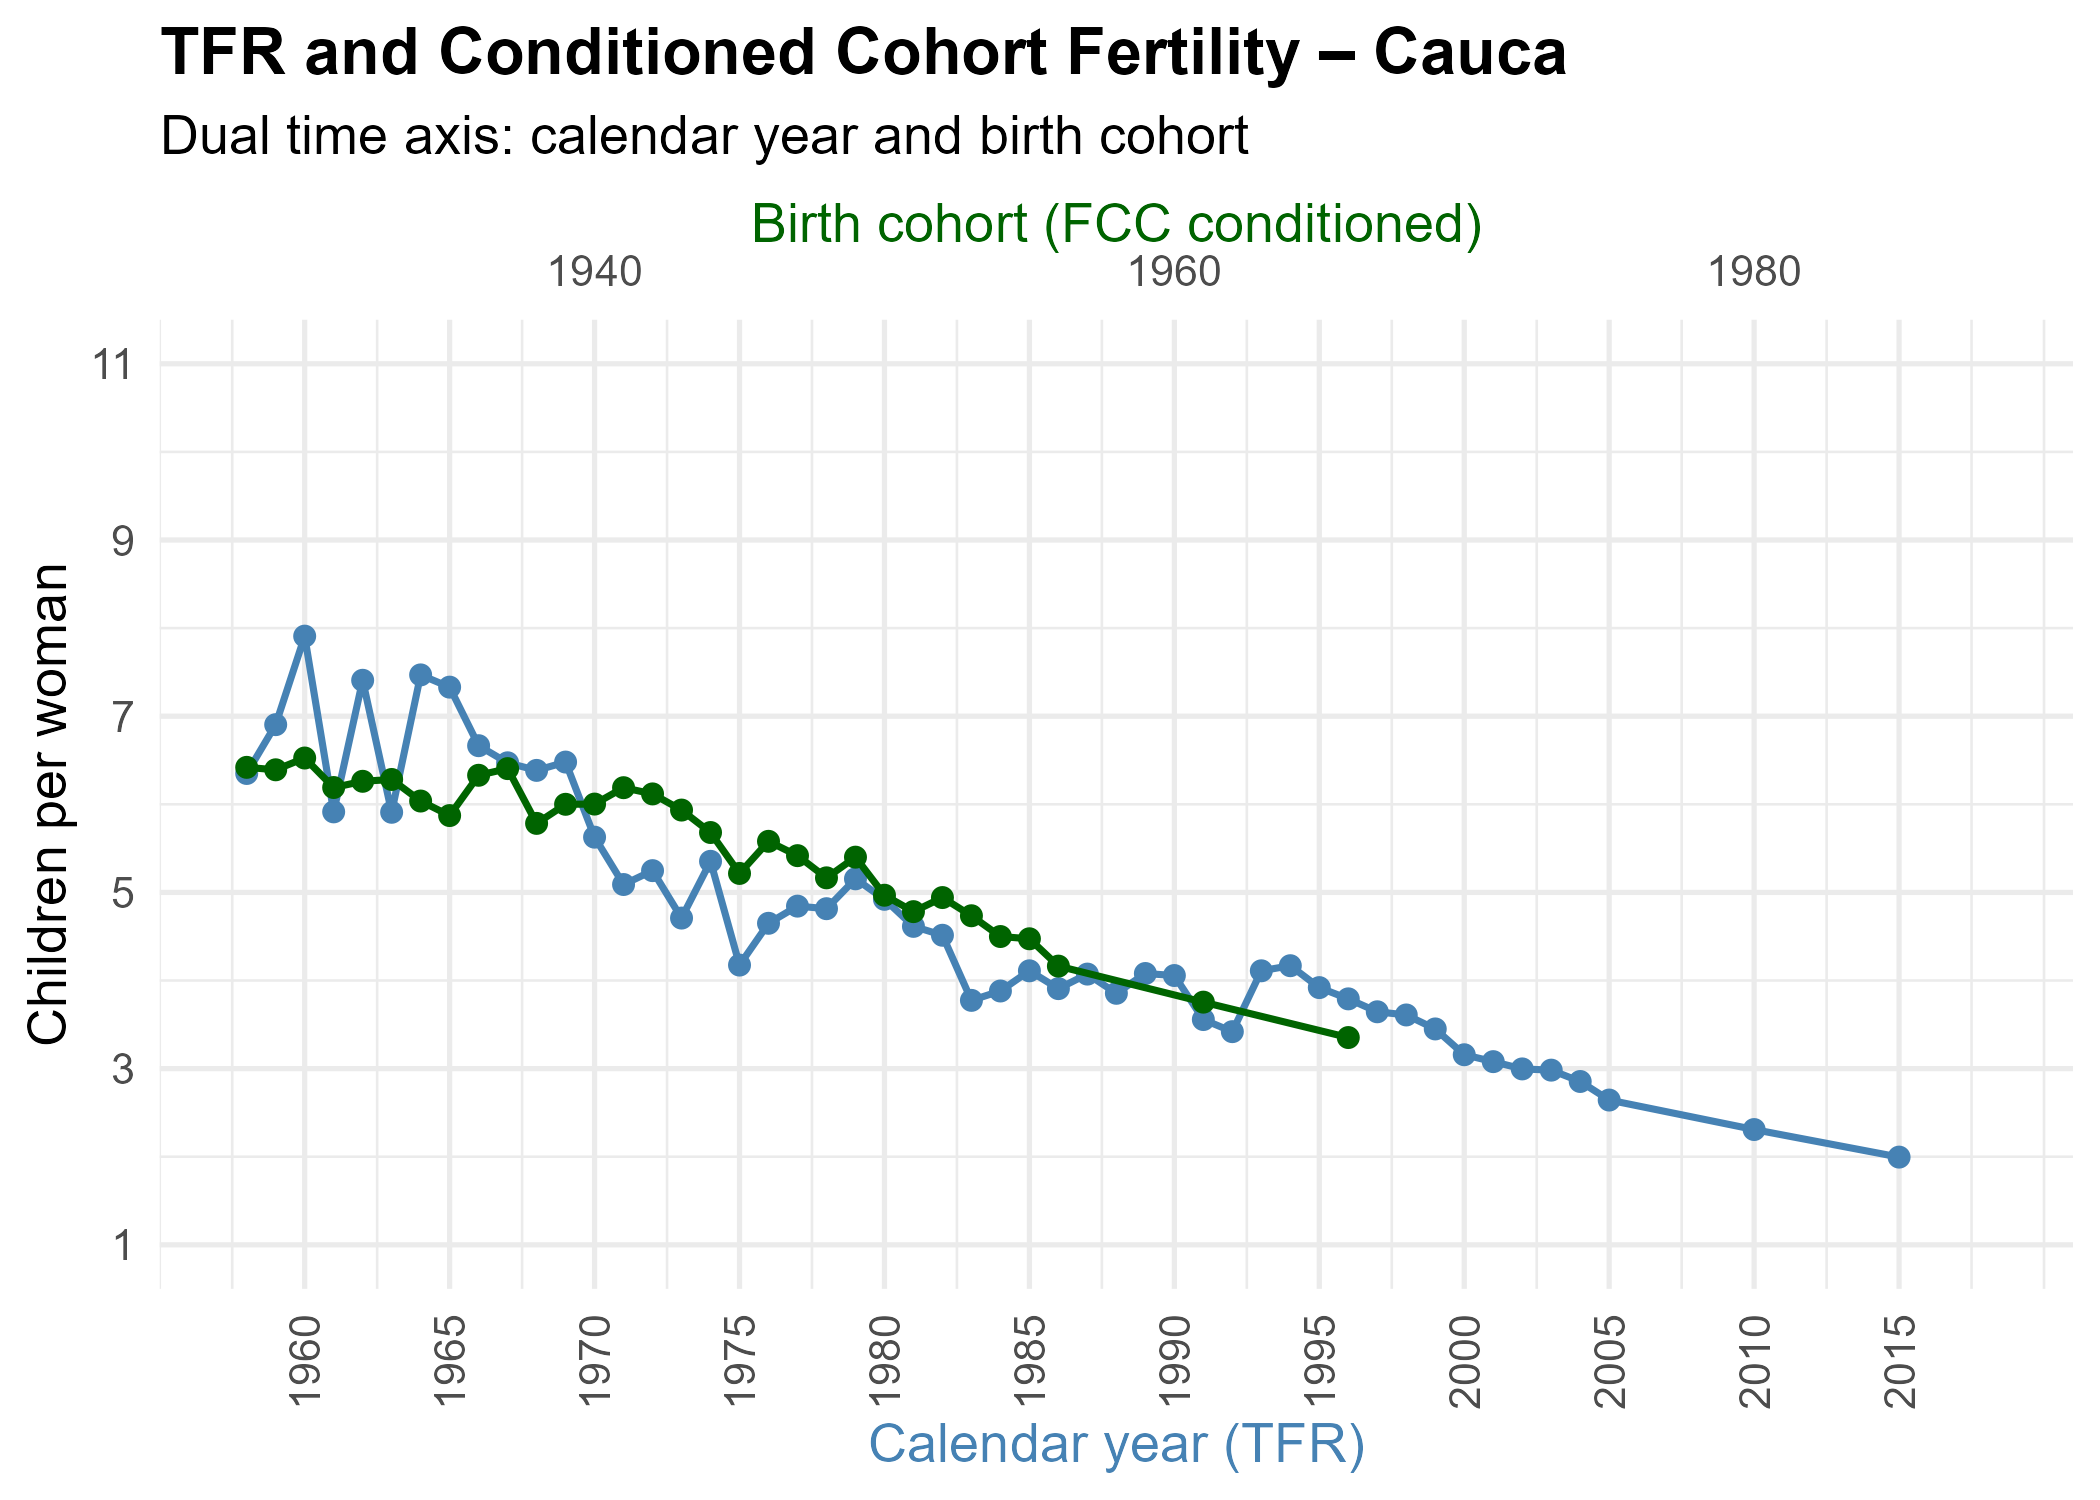
\includegraphics[height=0.78\textheight]{tfr_vs_fcc/TFR_FCCcond_Cauca.png}
\end{center}
\end{frame}
\begin{frame}{TGF vs.\ FCC: Cesar}
\begin{center}
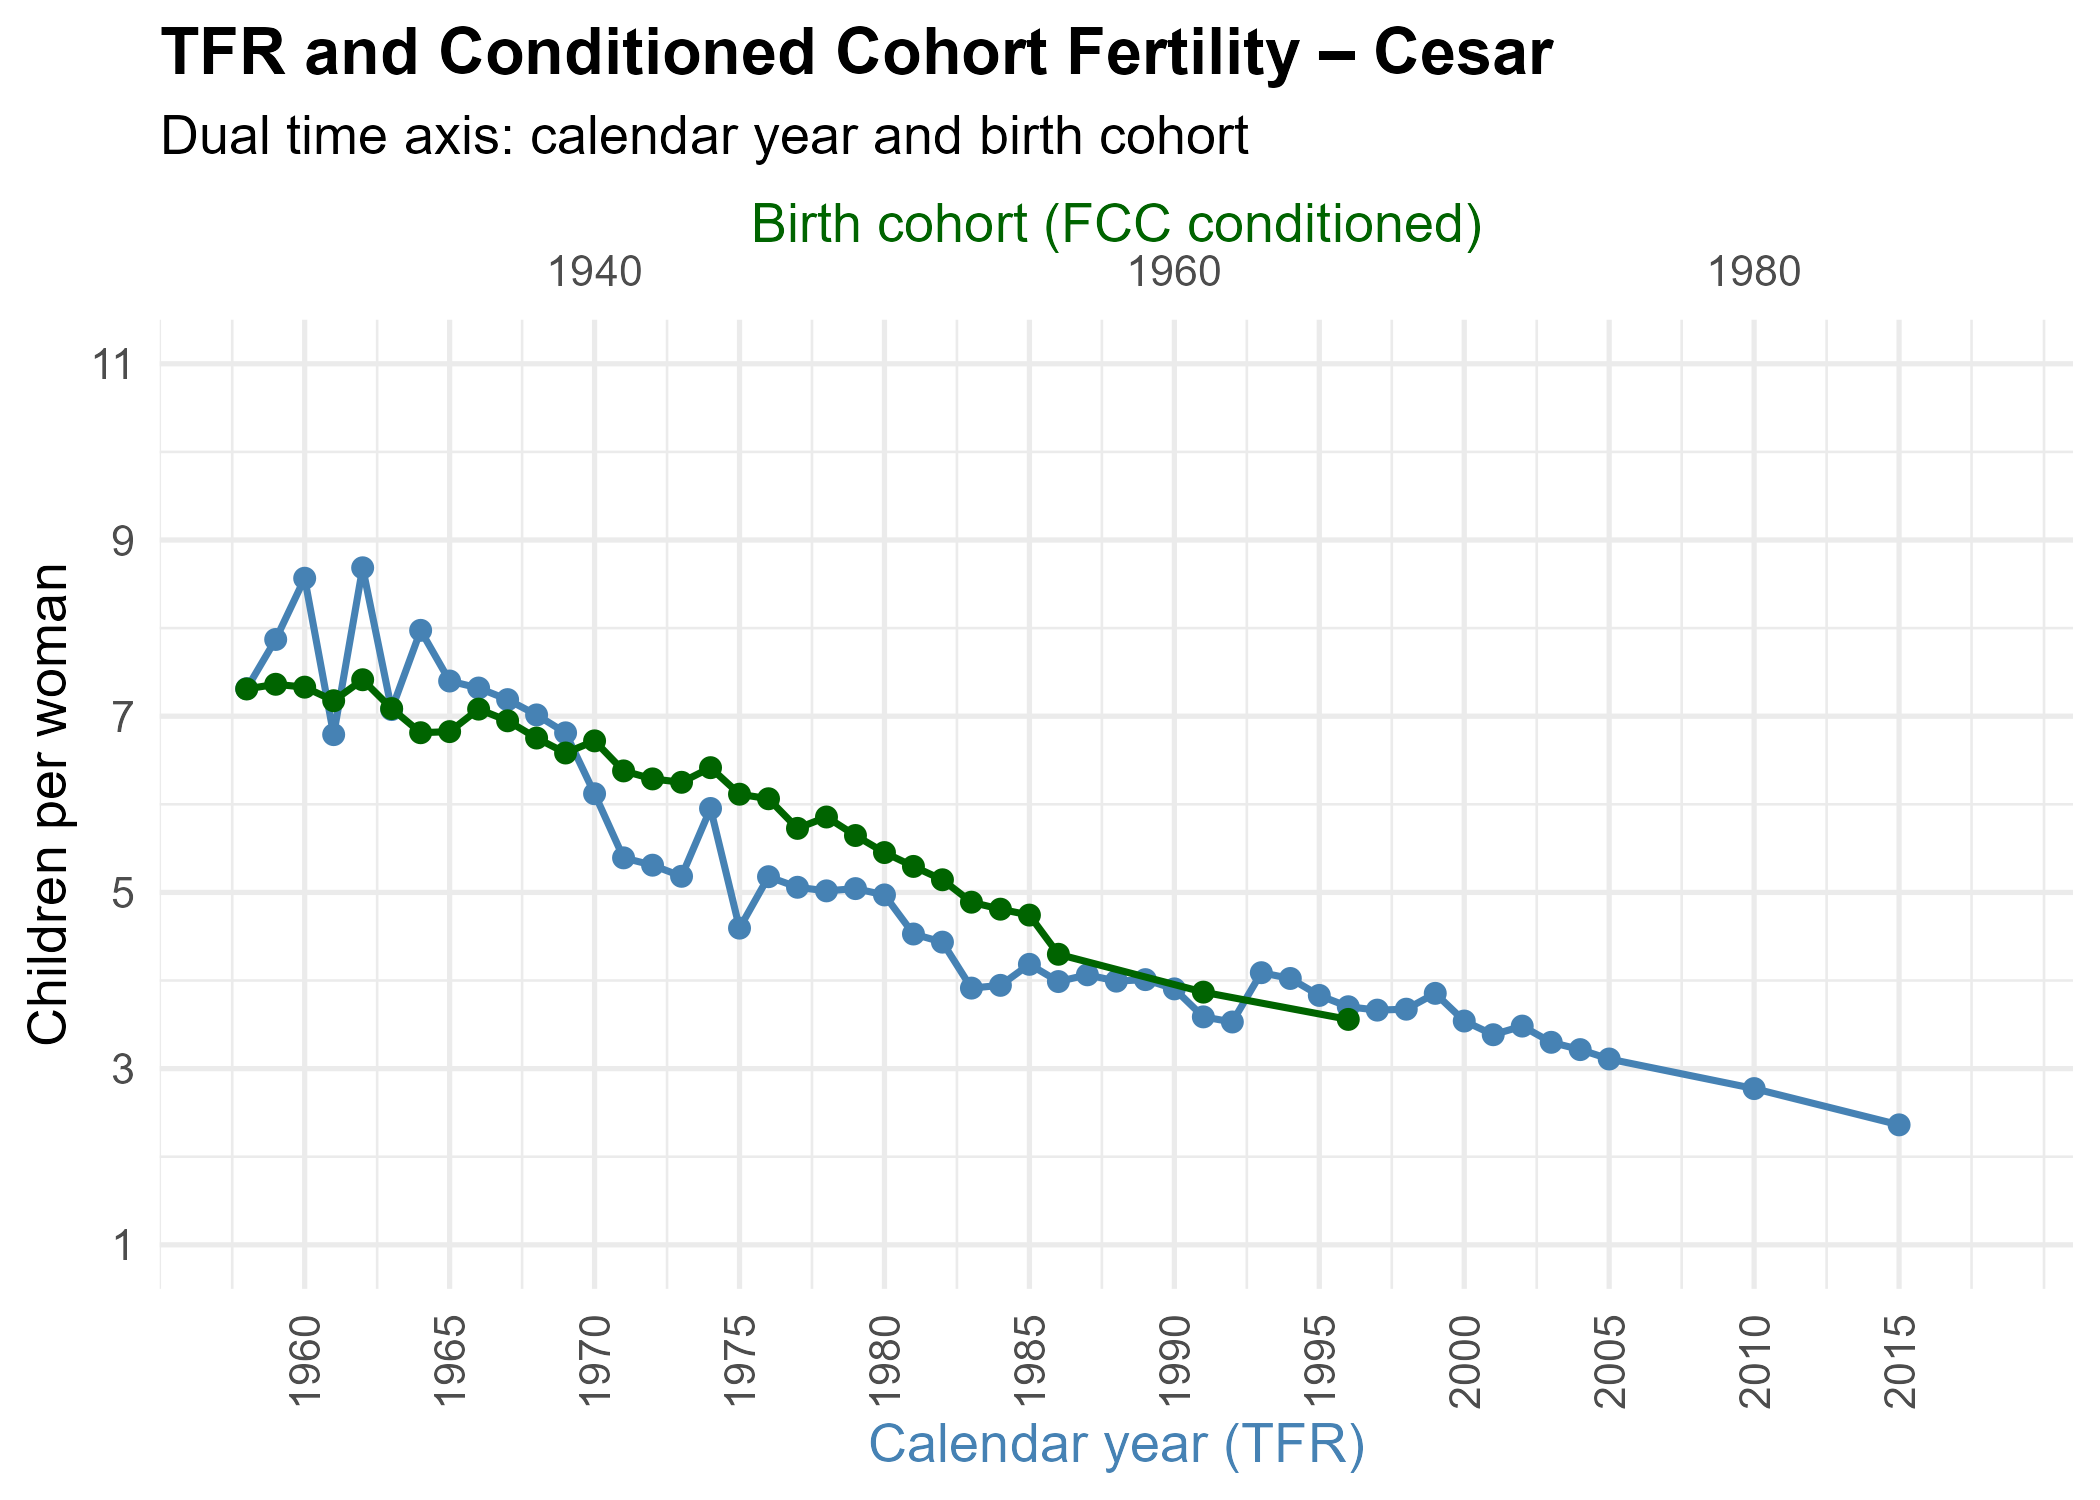
\includegraphics[height=0.78\textheight]{tfr_vs_fcc/TFR_FCCcond_Cesar.png}
\end{center}
\end{frame}
\begin{frame}{TGF vs.\ FCC: Chocó}
\begin{center}
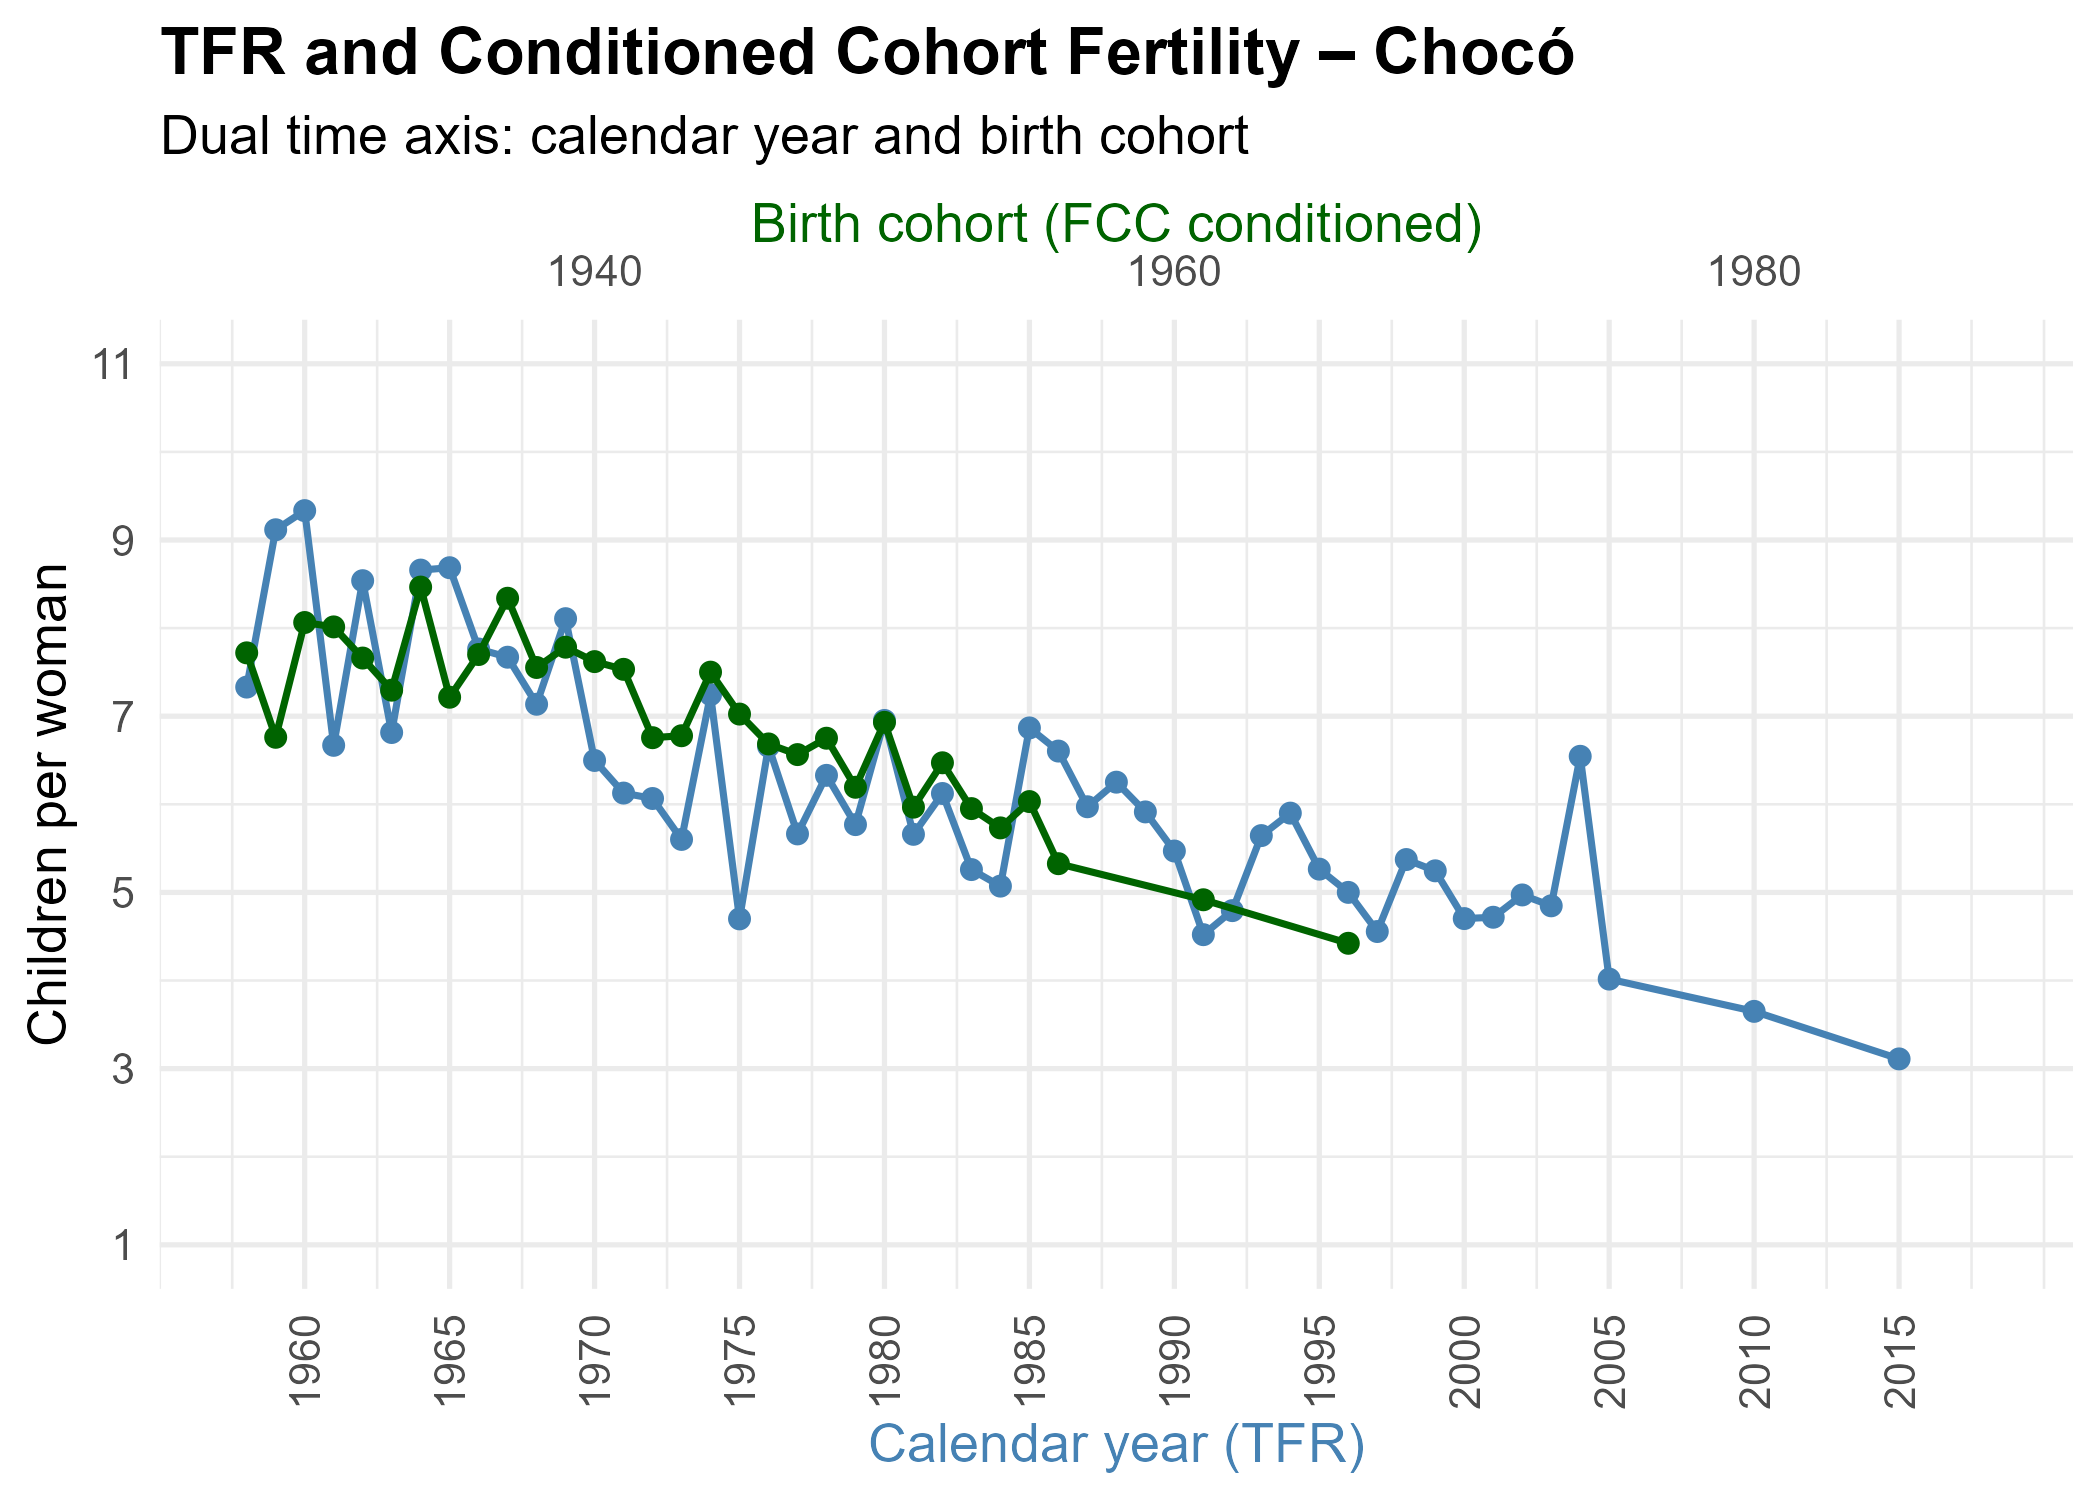
\includegraphics[height=0.78\textheight]{tfr_vs_fcc/TFR_FCCcond_Chocó.png}
\end{center}
\end{frame}
\begin{frame}{TGF vs.\ FCC: Córdoba}
\begin{center}
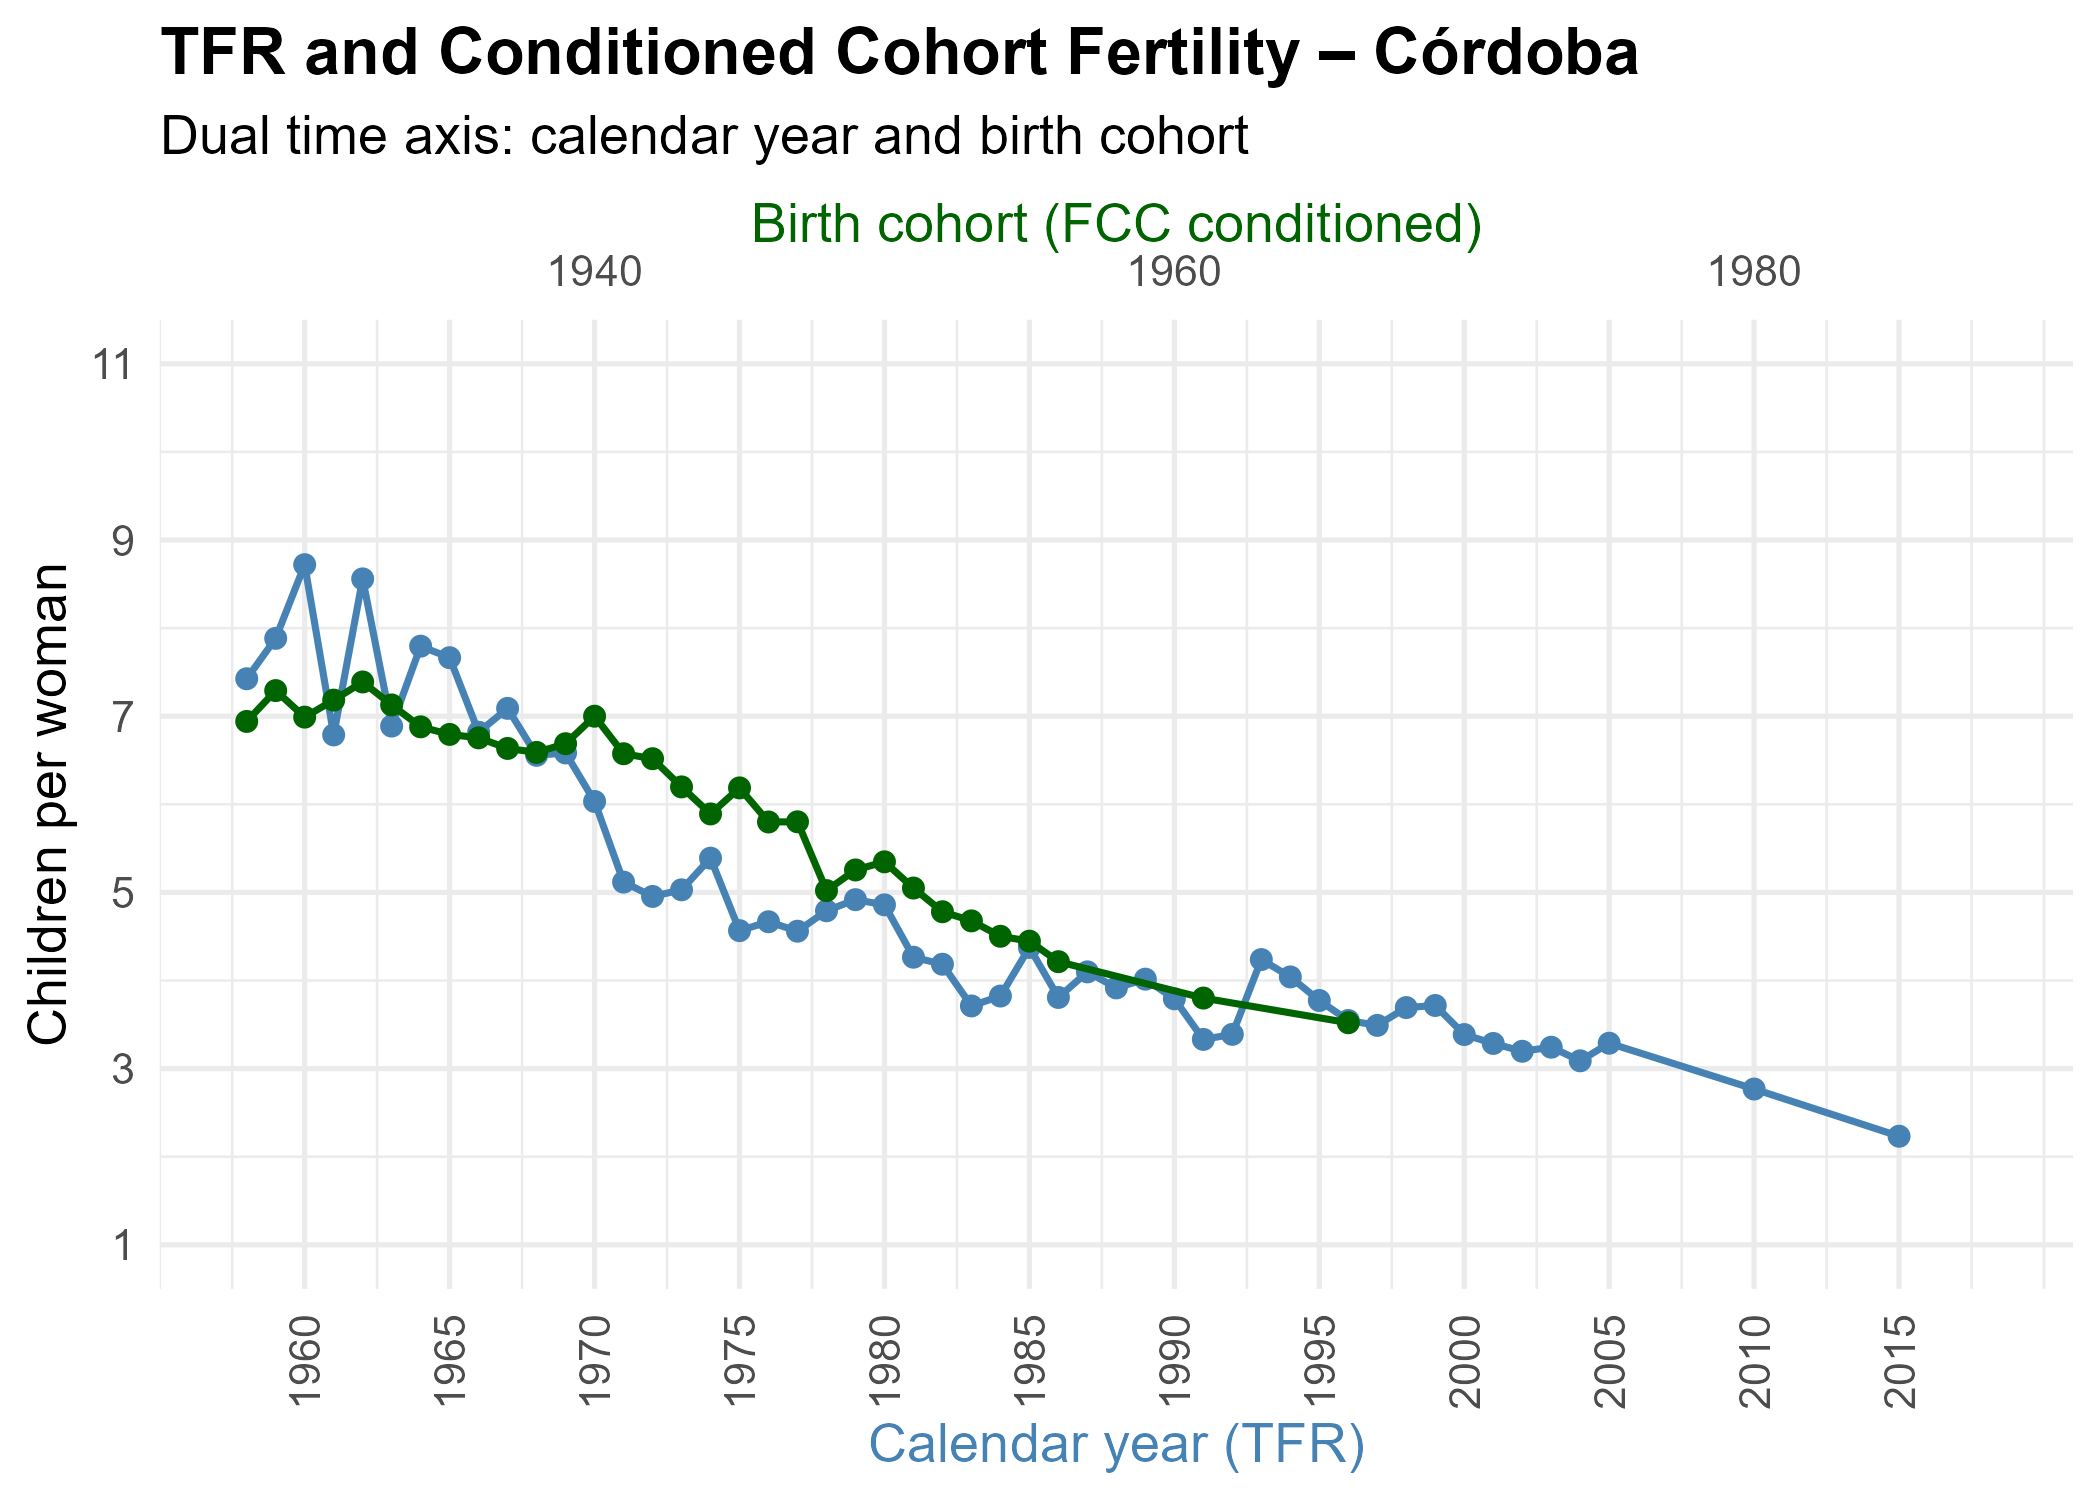
\includegraphics[height=0.78\textheight]{tfr_vs_fcc/TFR_FCCcond_Córdoba.png}
\end{center}
\end{frame}
\begin{frame}{TGF vs.\ FCC: Huila}
\begin{center}
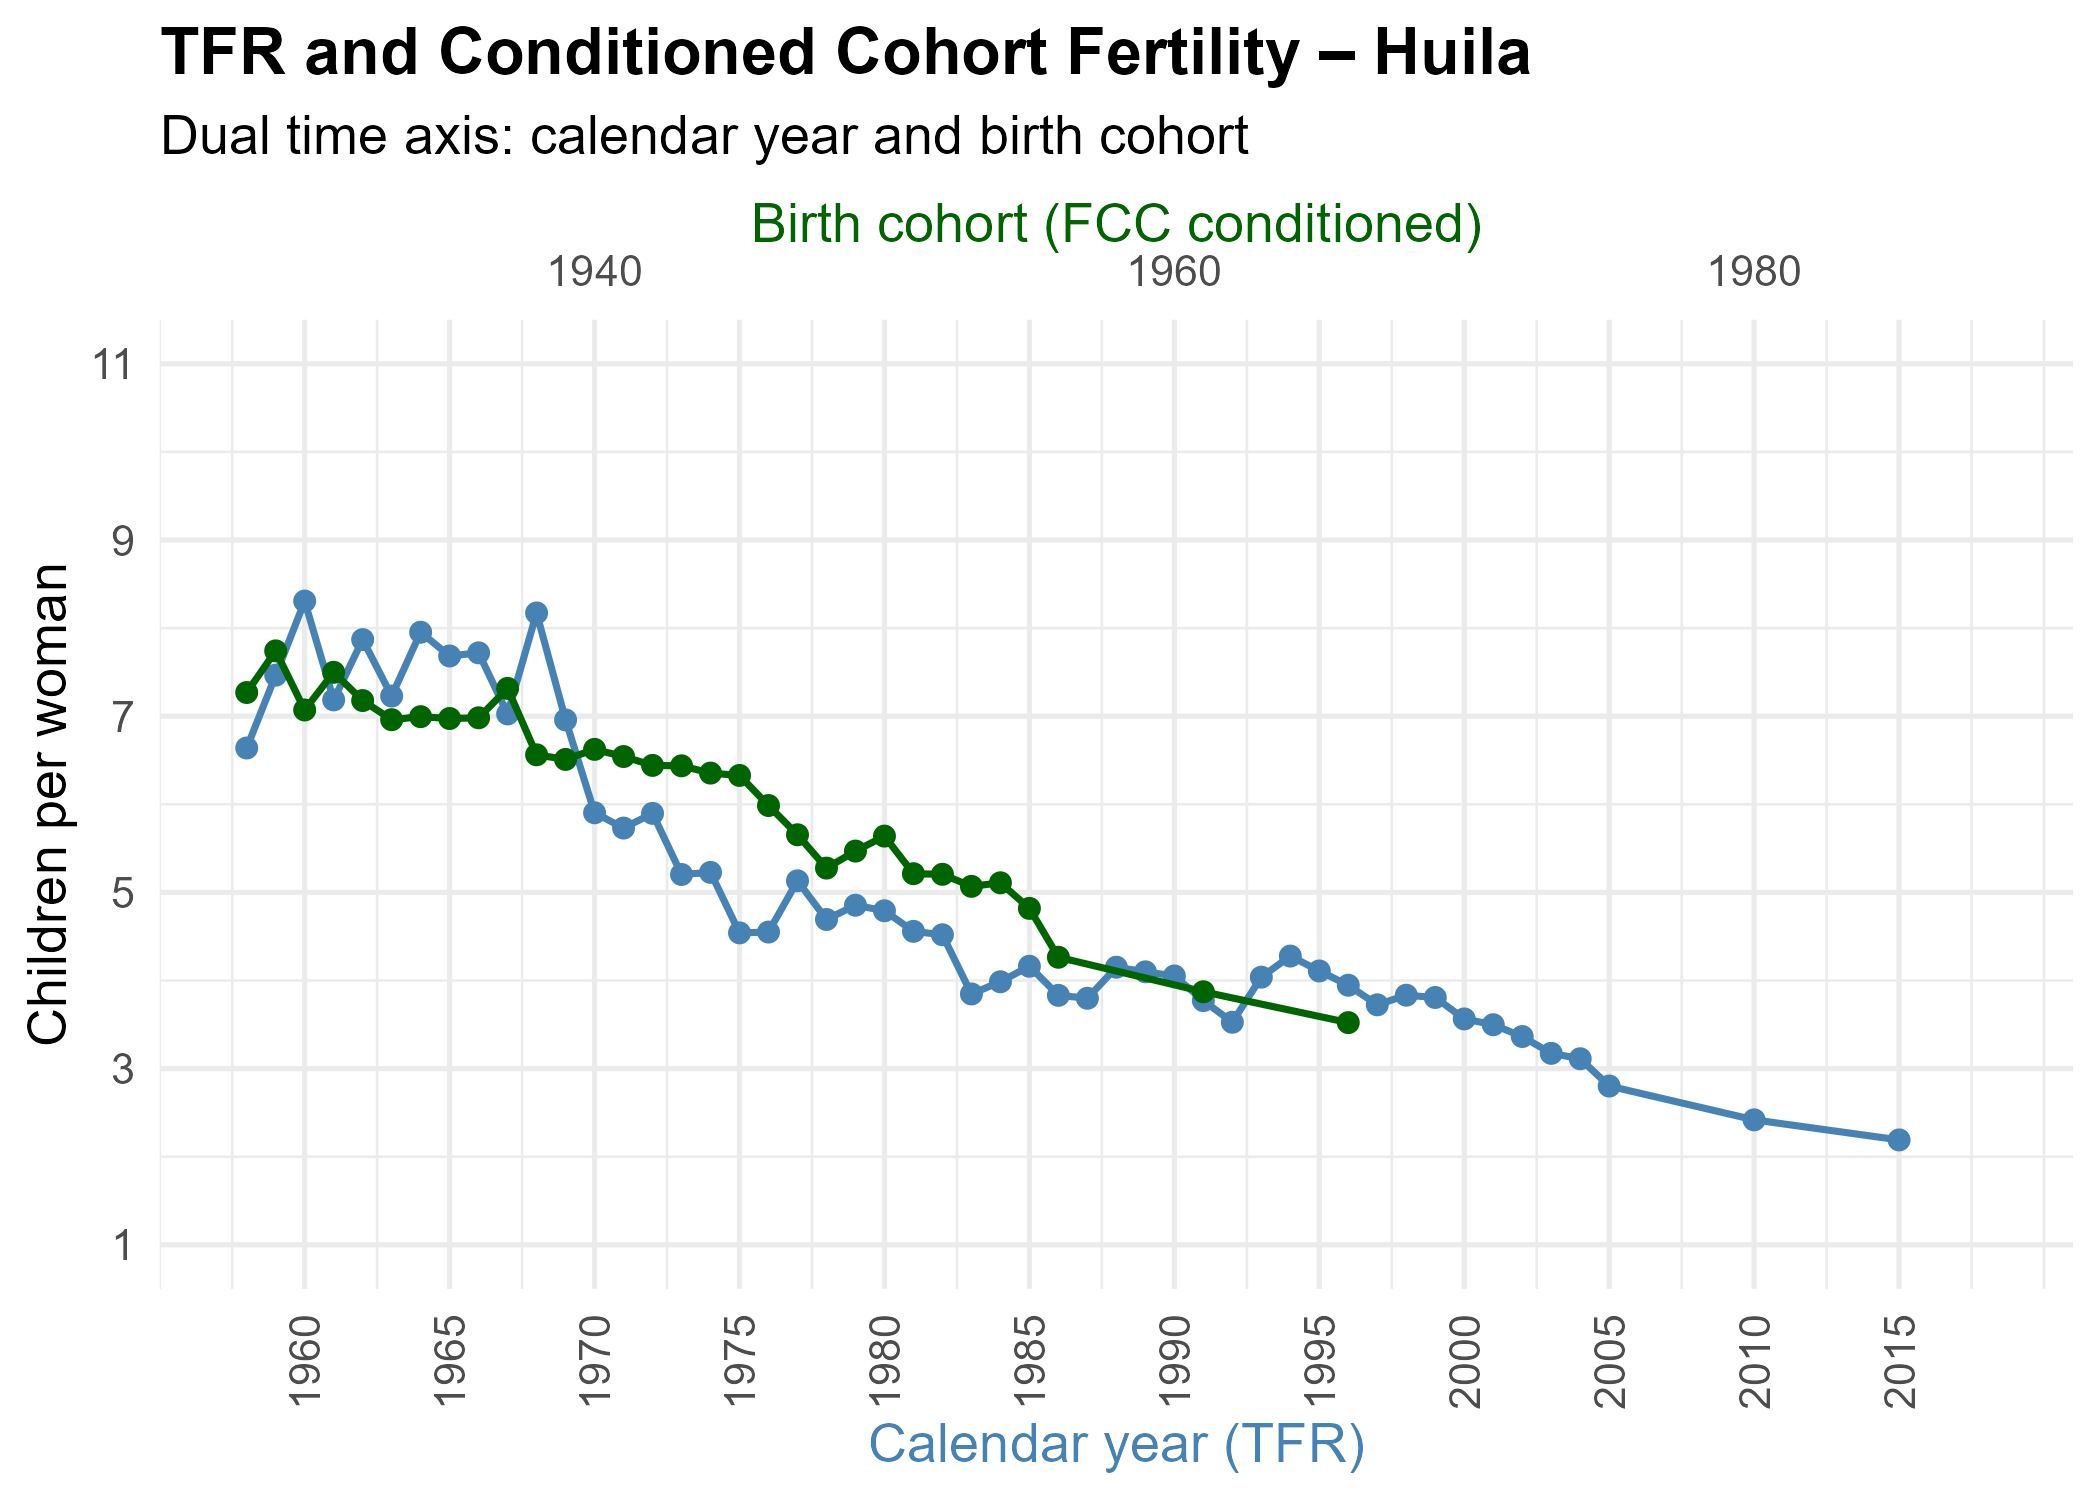
\includegraphics[height=0.78\textheight]{tfr_vs_fcc/TFR_FCCcond_Huila.png}
\end{center}
\end{frame}
\begin{frame}{TGF vs.\ FCC: La Guajira}
\begin{center}
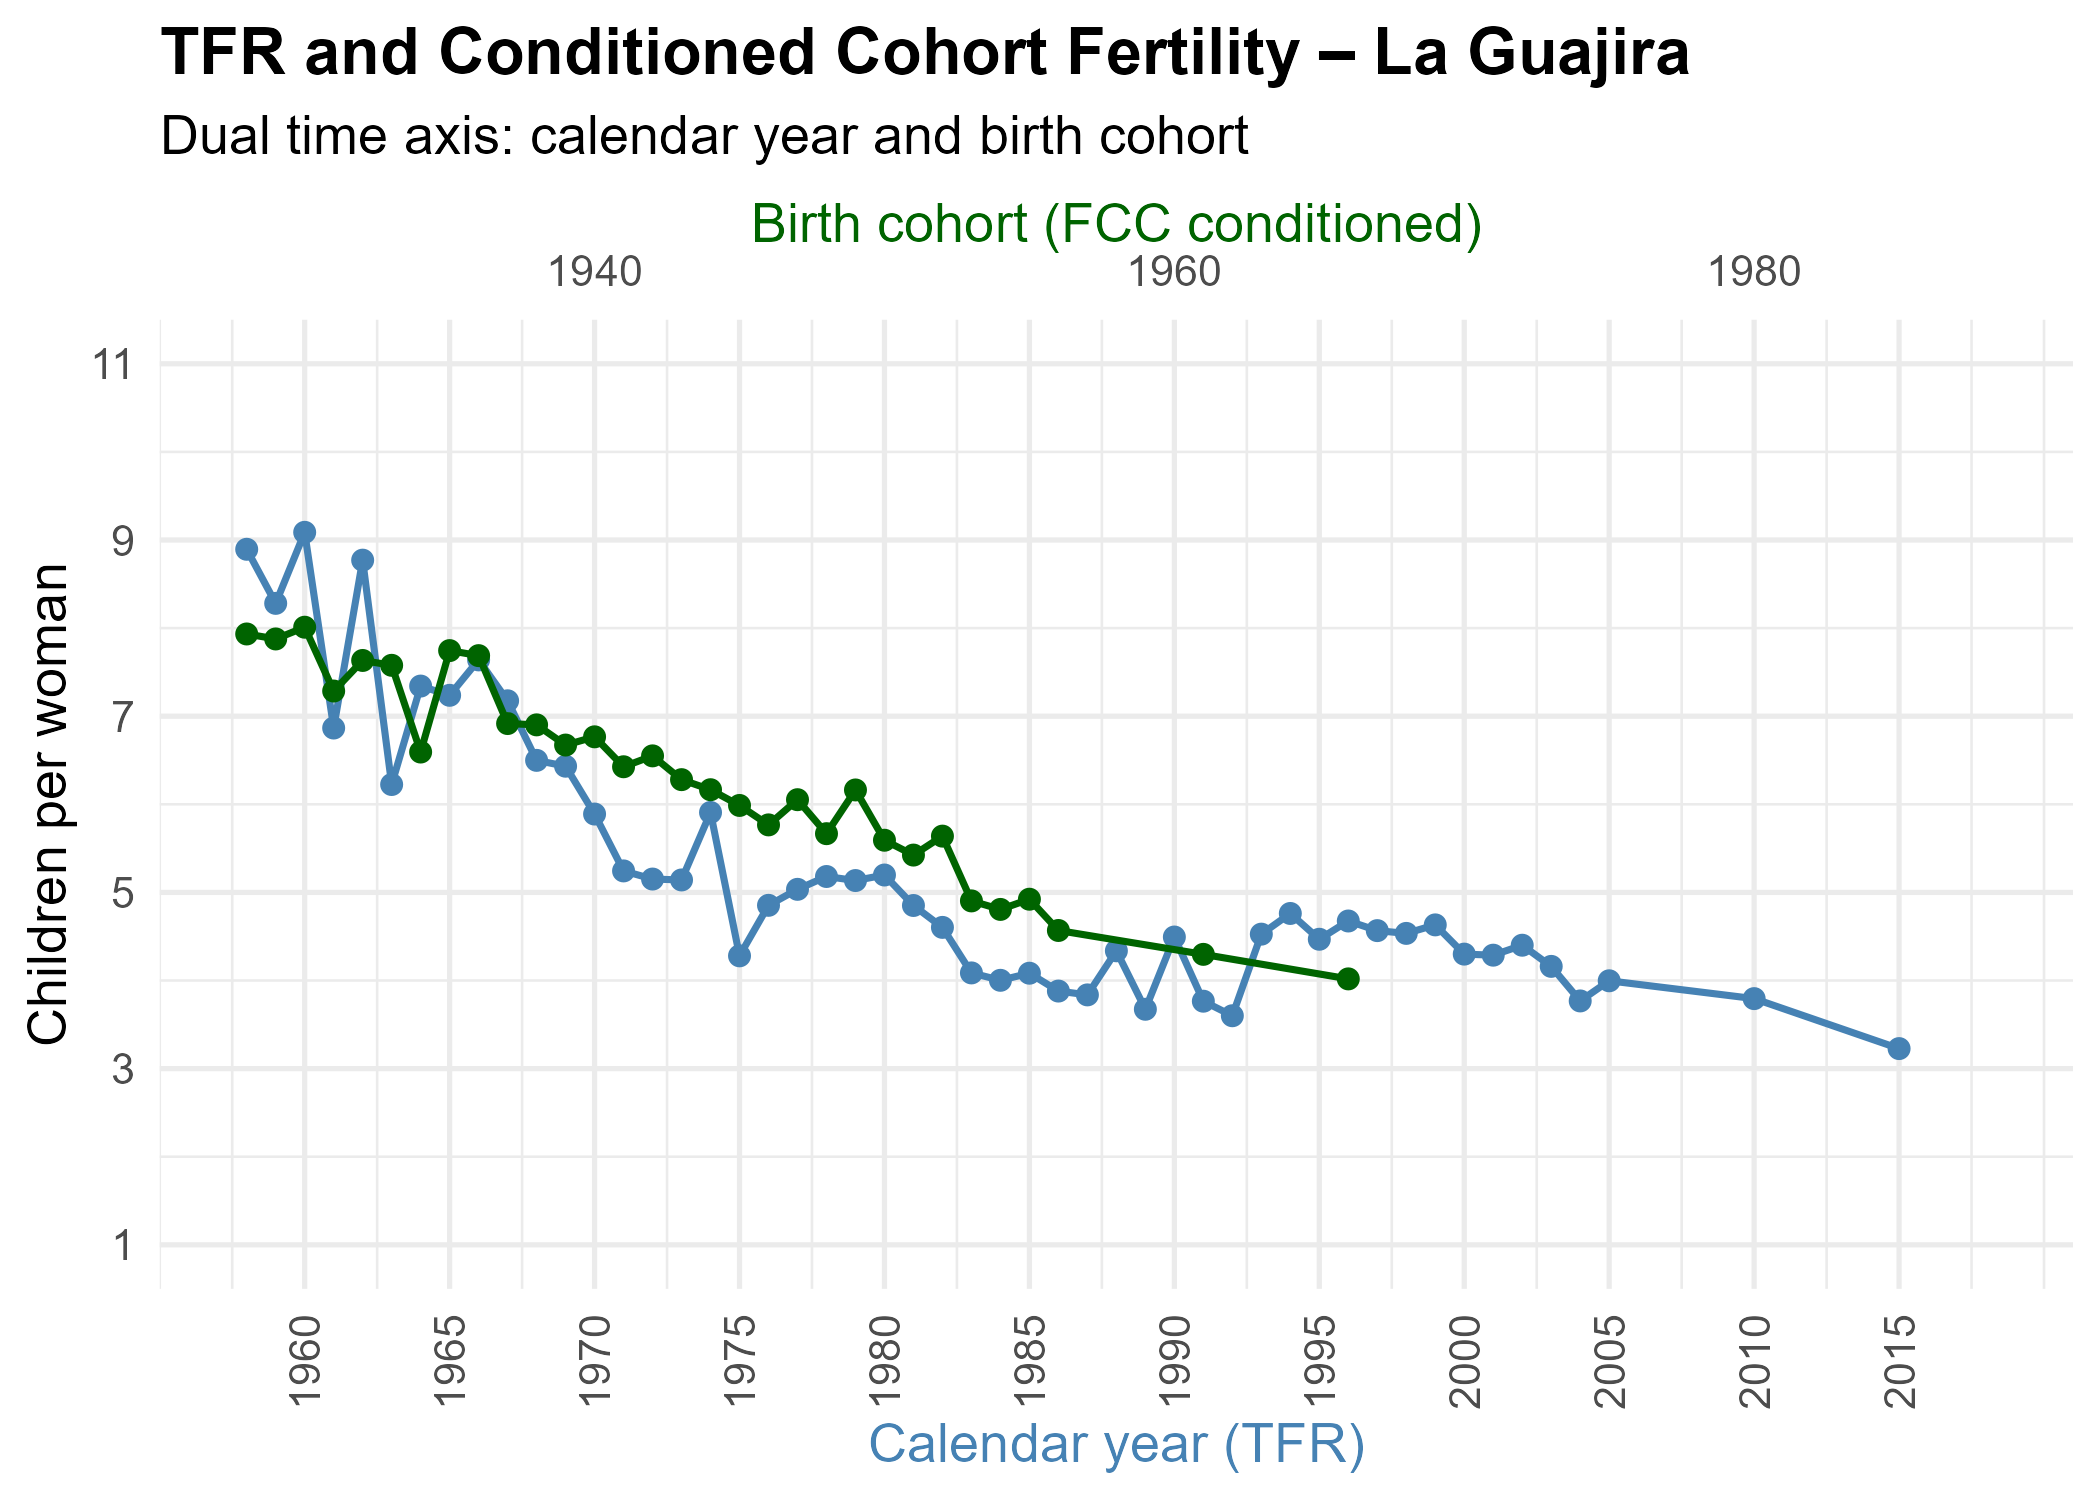
\includegraphics[height=0.78\textheight]{tfr_vs_fcc/TFR_FCCcond_La Guajira.png}
\end{center}
\end{frame}
\begin{frame}{TGF vs.\ FCC: Meta}
\begin{center}
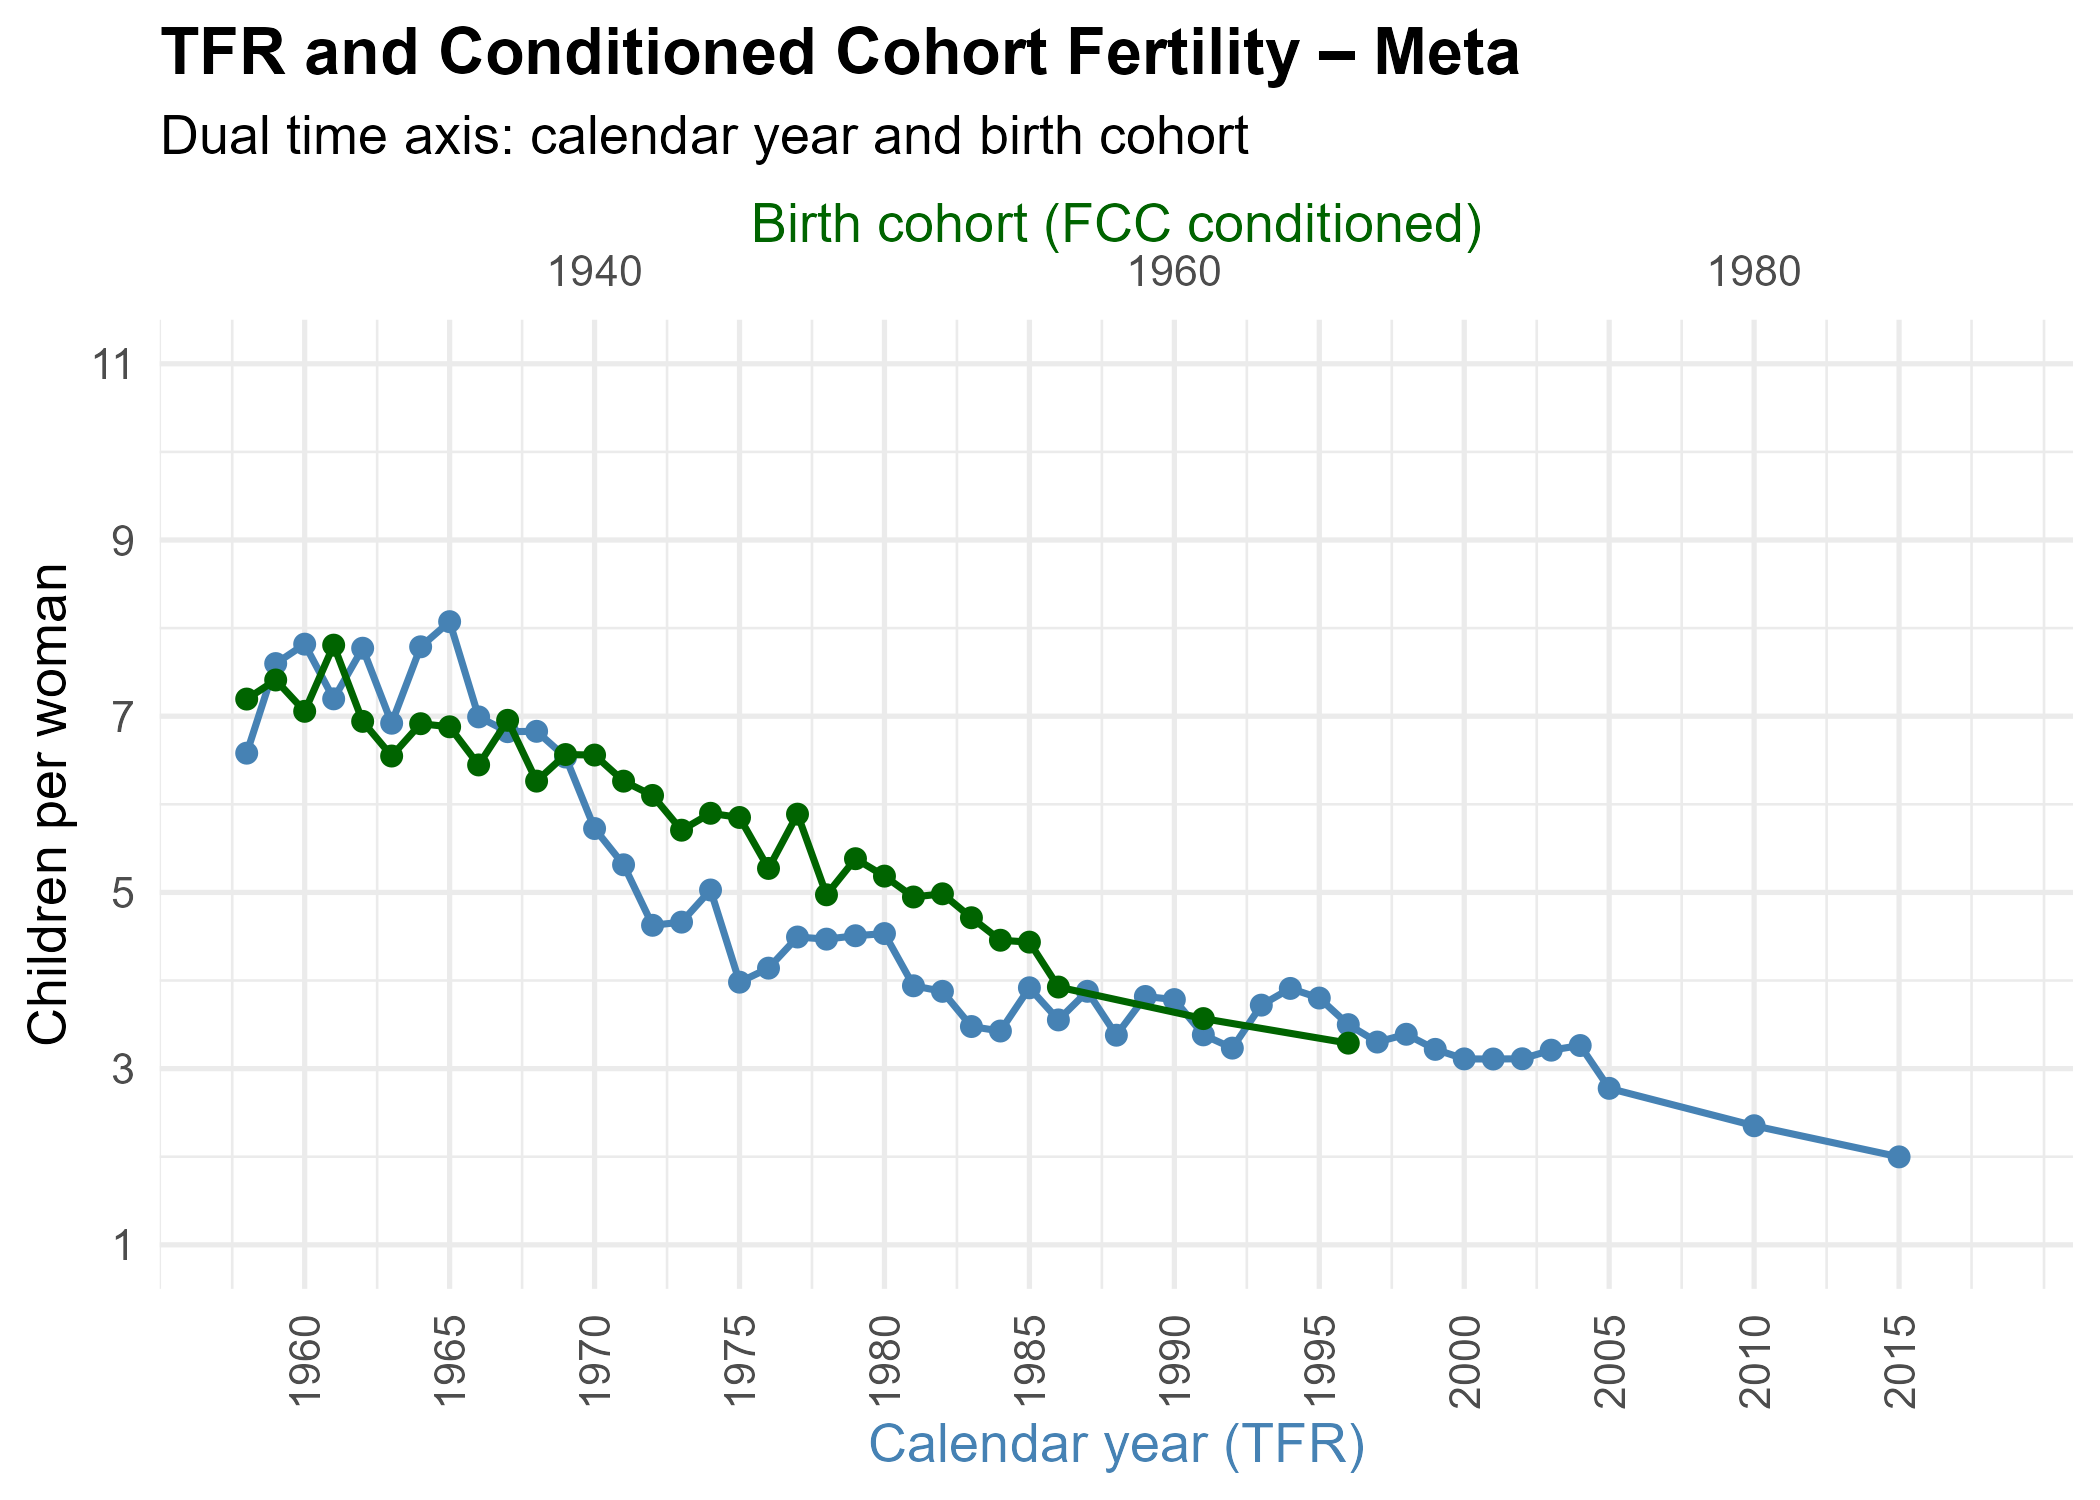
\includegraphics[height=0.78\textheight]{tfr_vs_fcc/TFR_FCCcond_Meta.png}
\end{center}
\end{frame}
\begin{frame}{TGF vs.\ FCC: Nariño}
\begin{center}
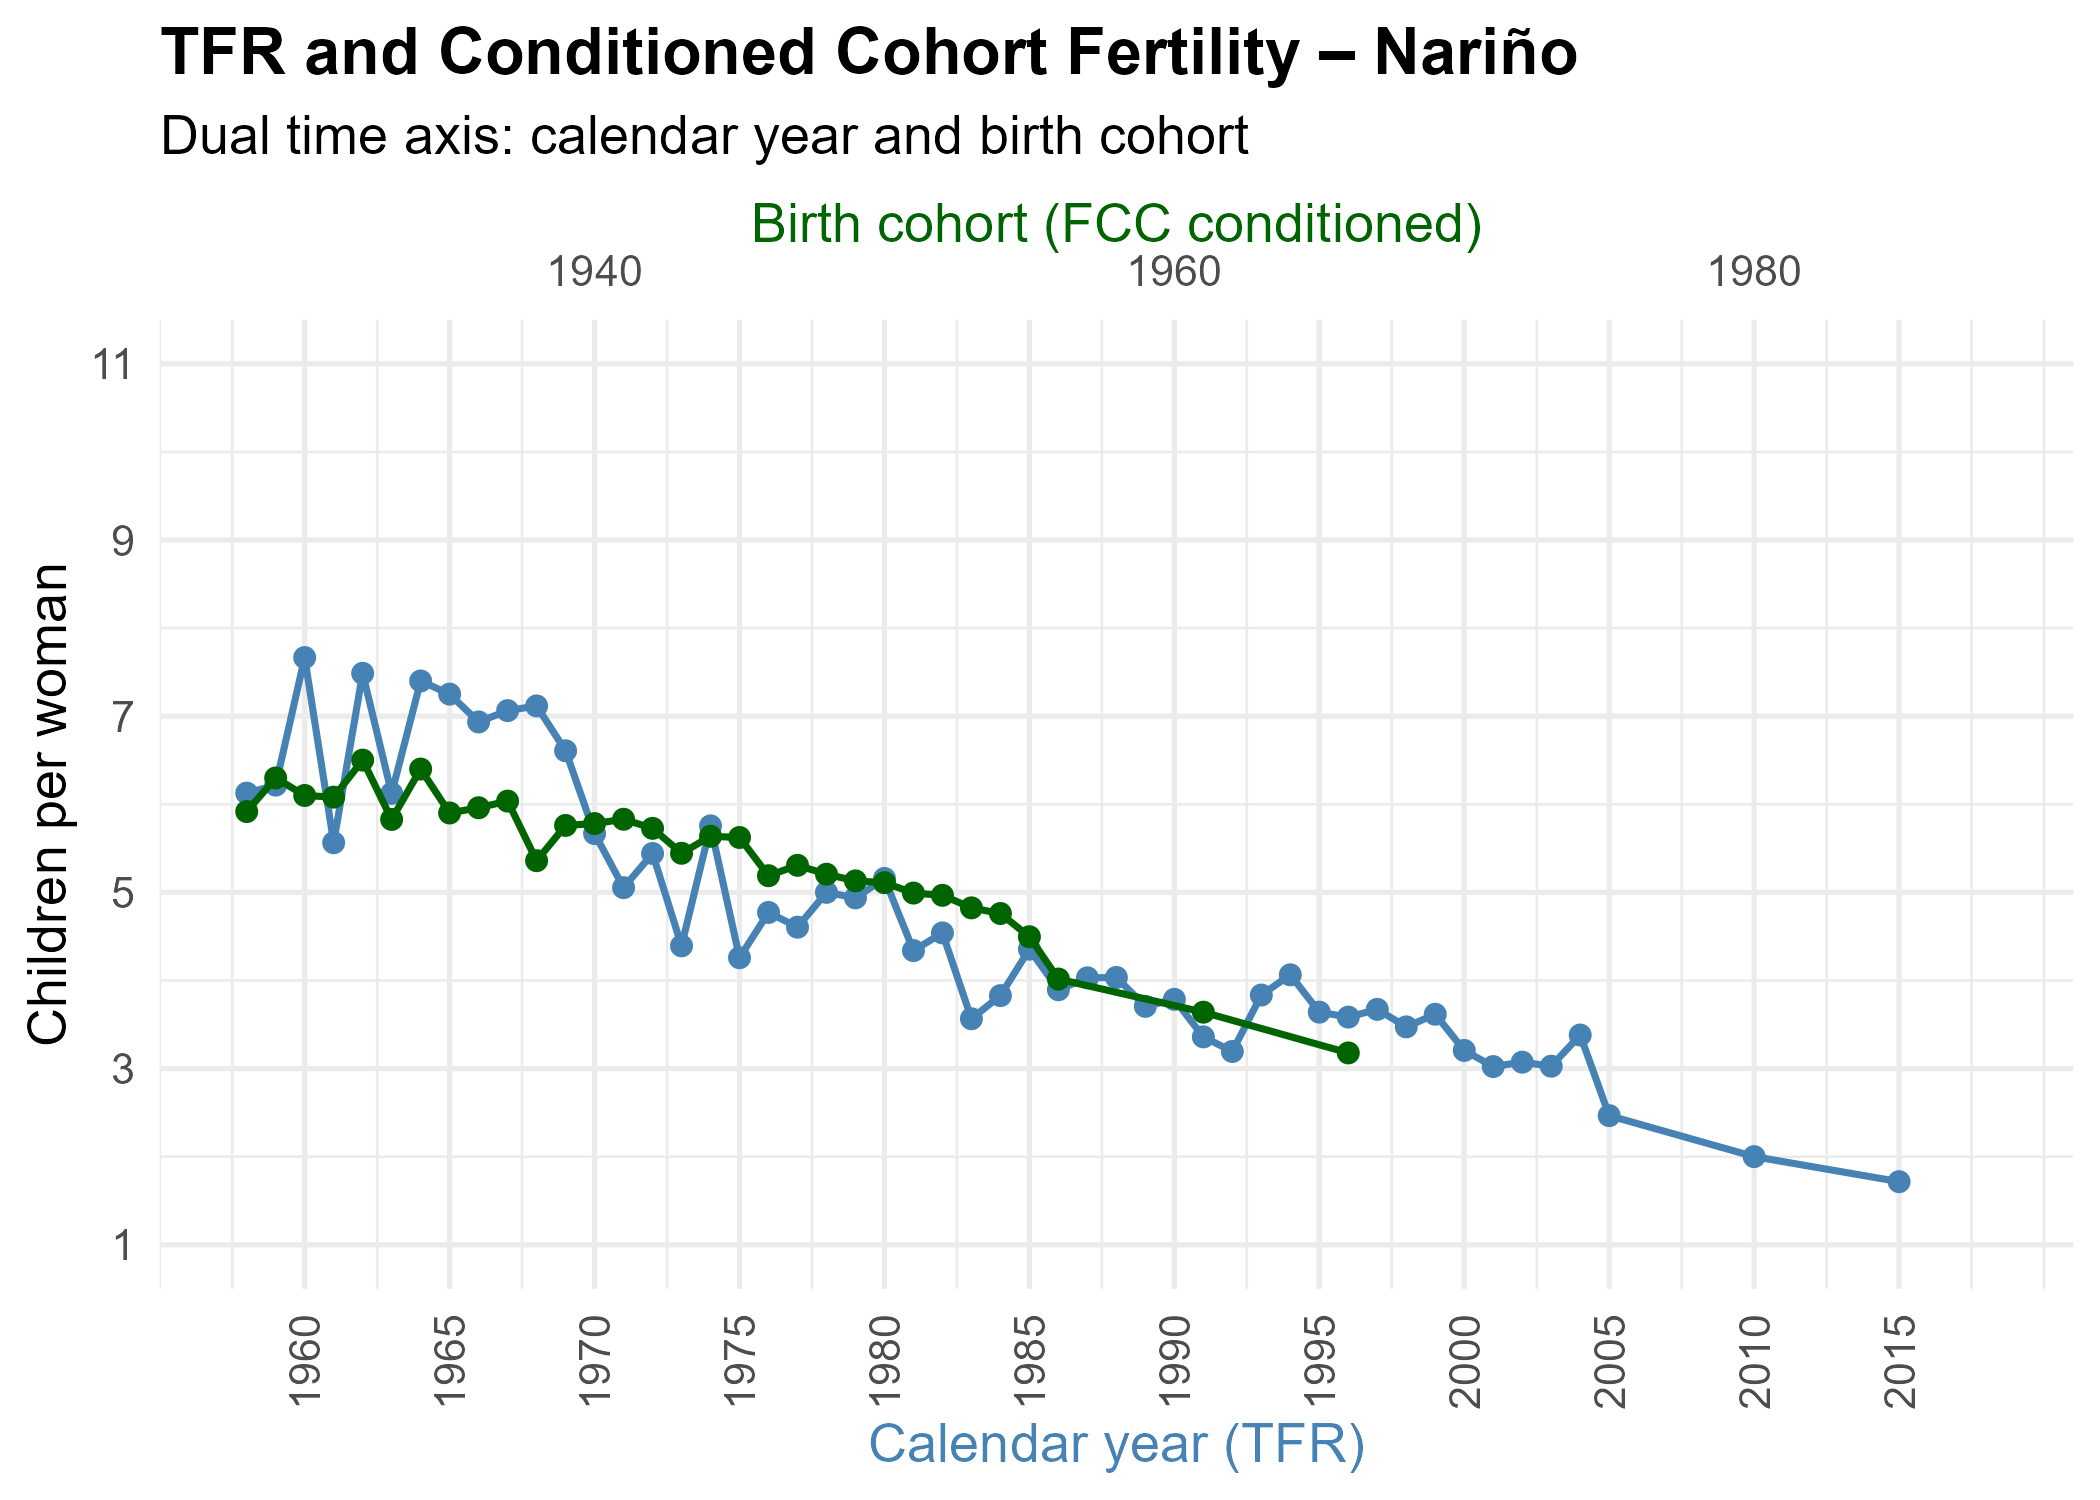
\includegraphics[height=0.78\textheight]{tfr_vs_fcc/TFR_FCCcond_Nariño.png}
\end{center}
\end{frame}
\begin{frame}{TGF vs.\ FCC: Putumayo}
\begin{center}
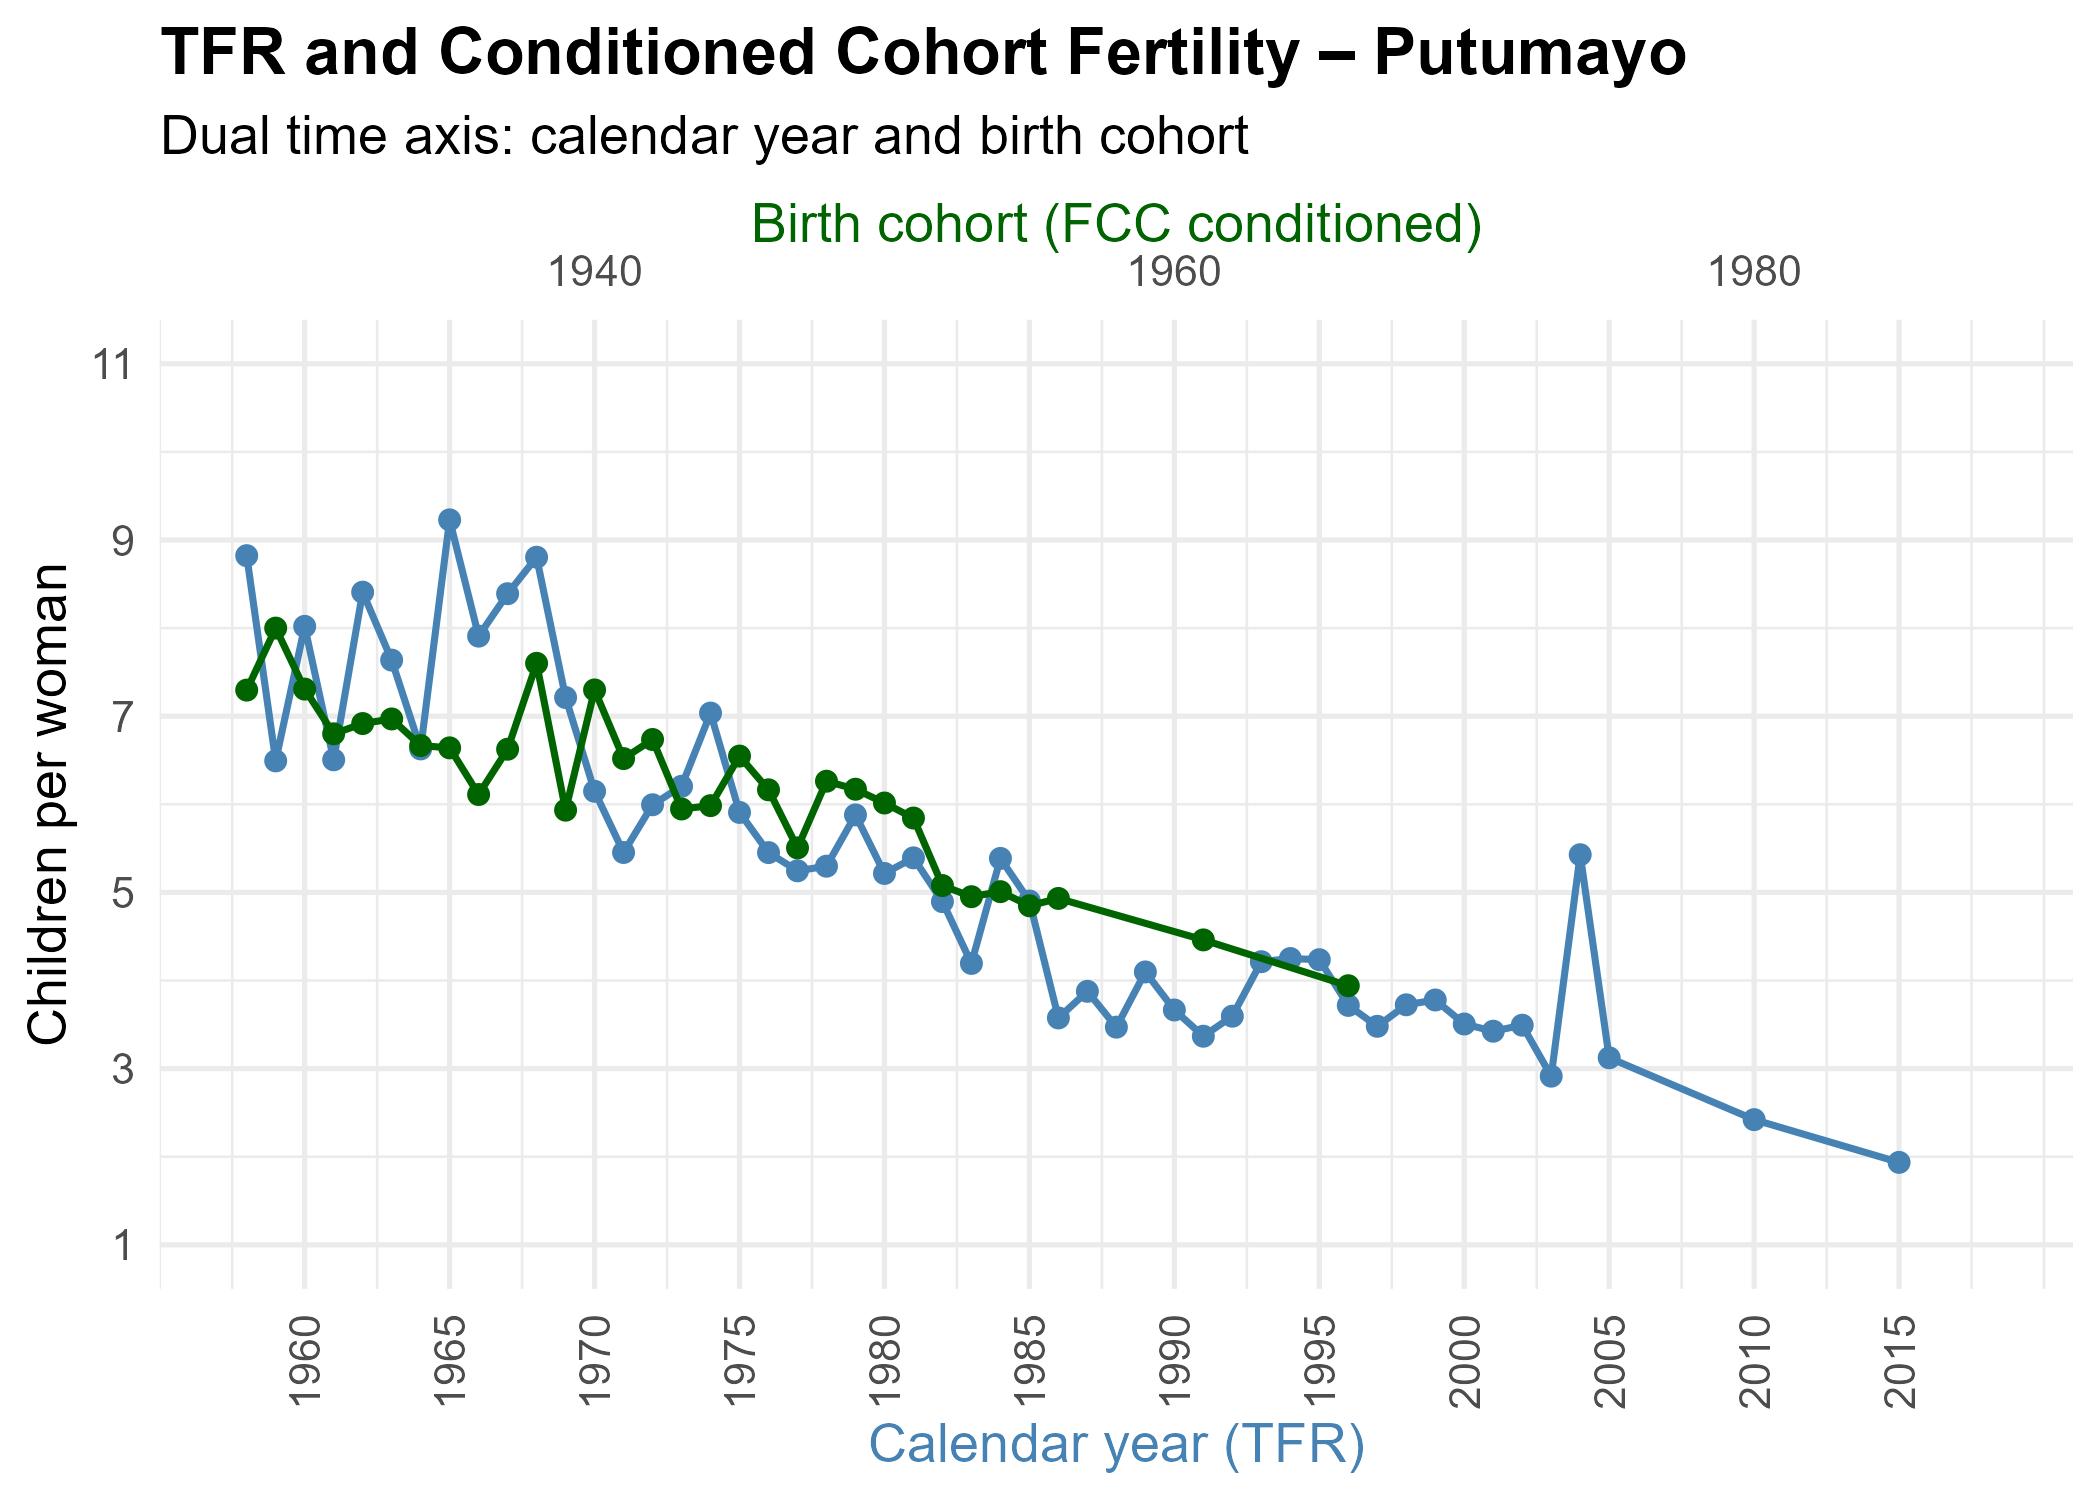
\includegraphics[height=0.78\textheight]{tfr_vs_fcc/TFR_FCCcond_Putumayo.png}
\end{center}
\end{frame}
\begin{frame}{TGF vs.\ FCC: San Andrés}
\begin{center}
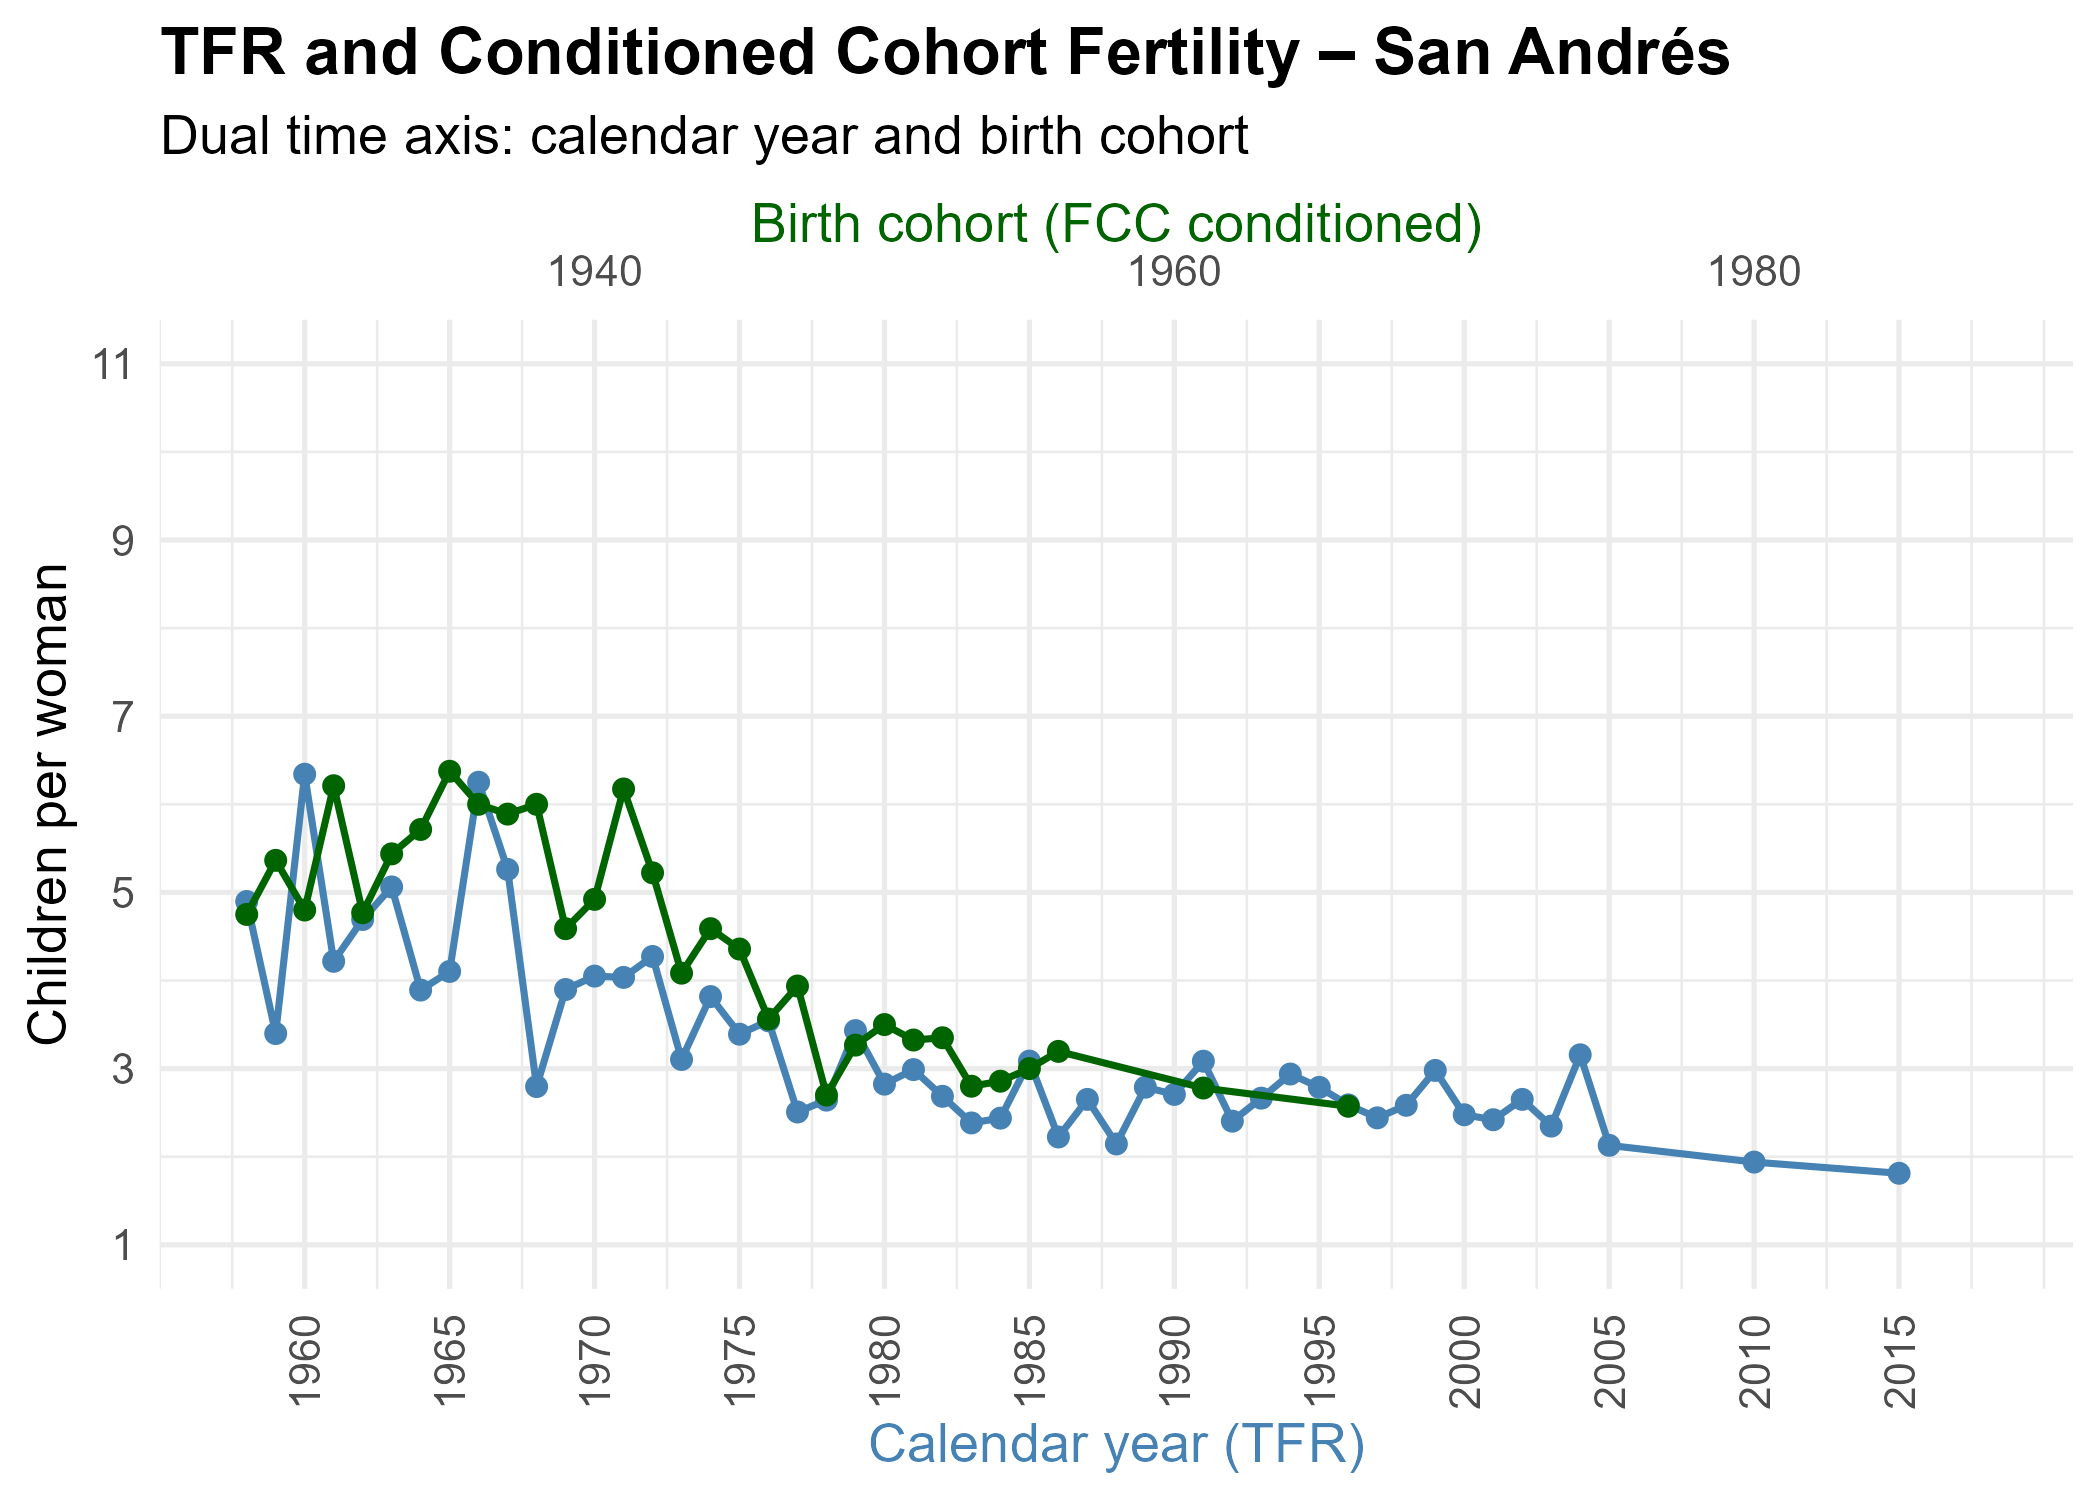
\includegraphics[height=0.78\textheight]{tfr_vs_fcc/TFR_FCCcond_San Andrés.png}
\end{center}
\end{frame}
\begin{frame}{TGF vs.\ FCC: Santander}
\begin{center}
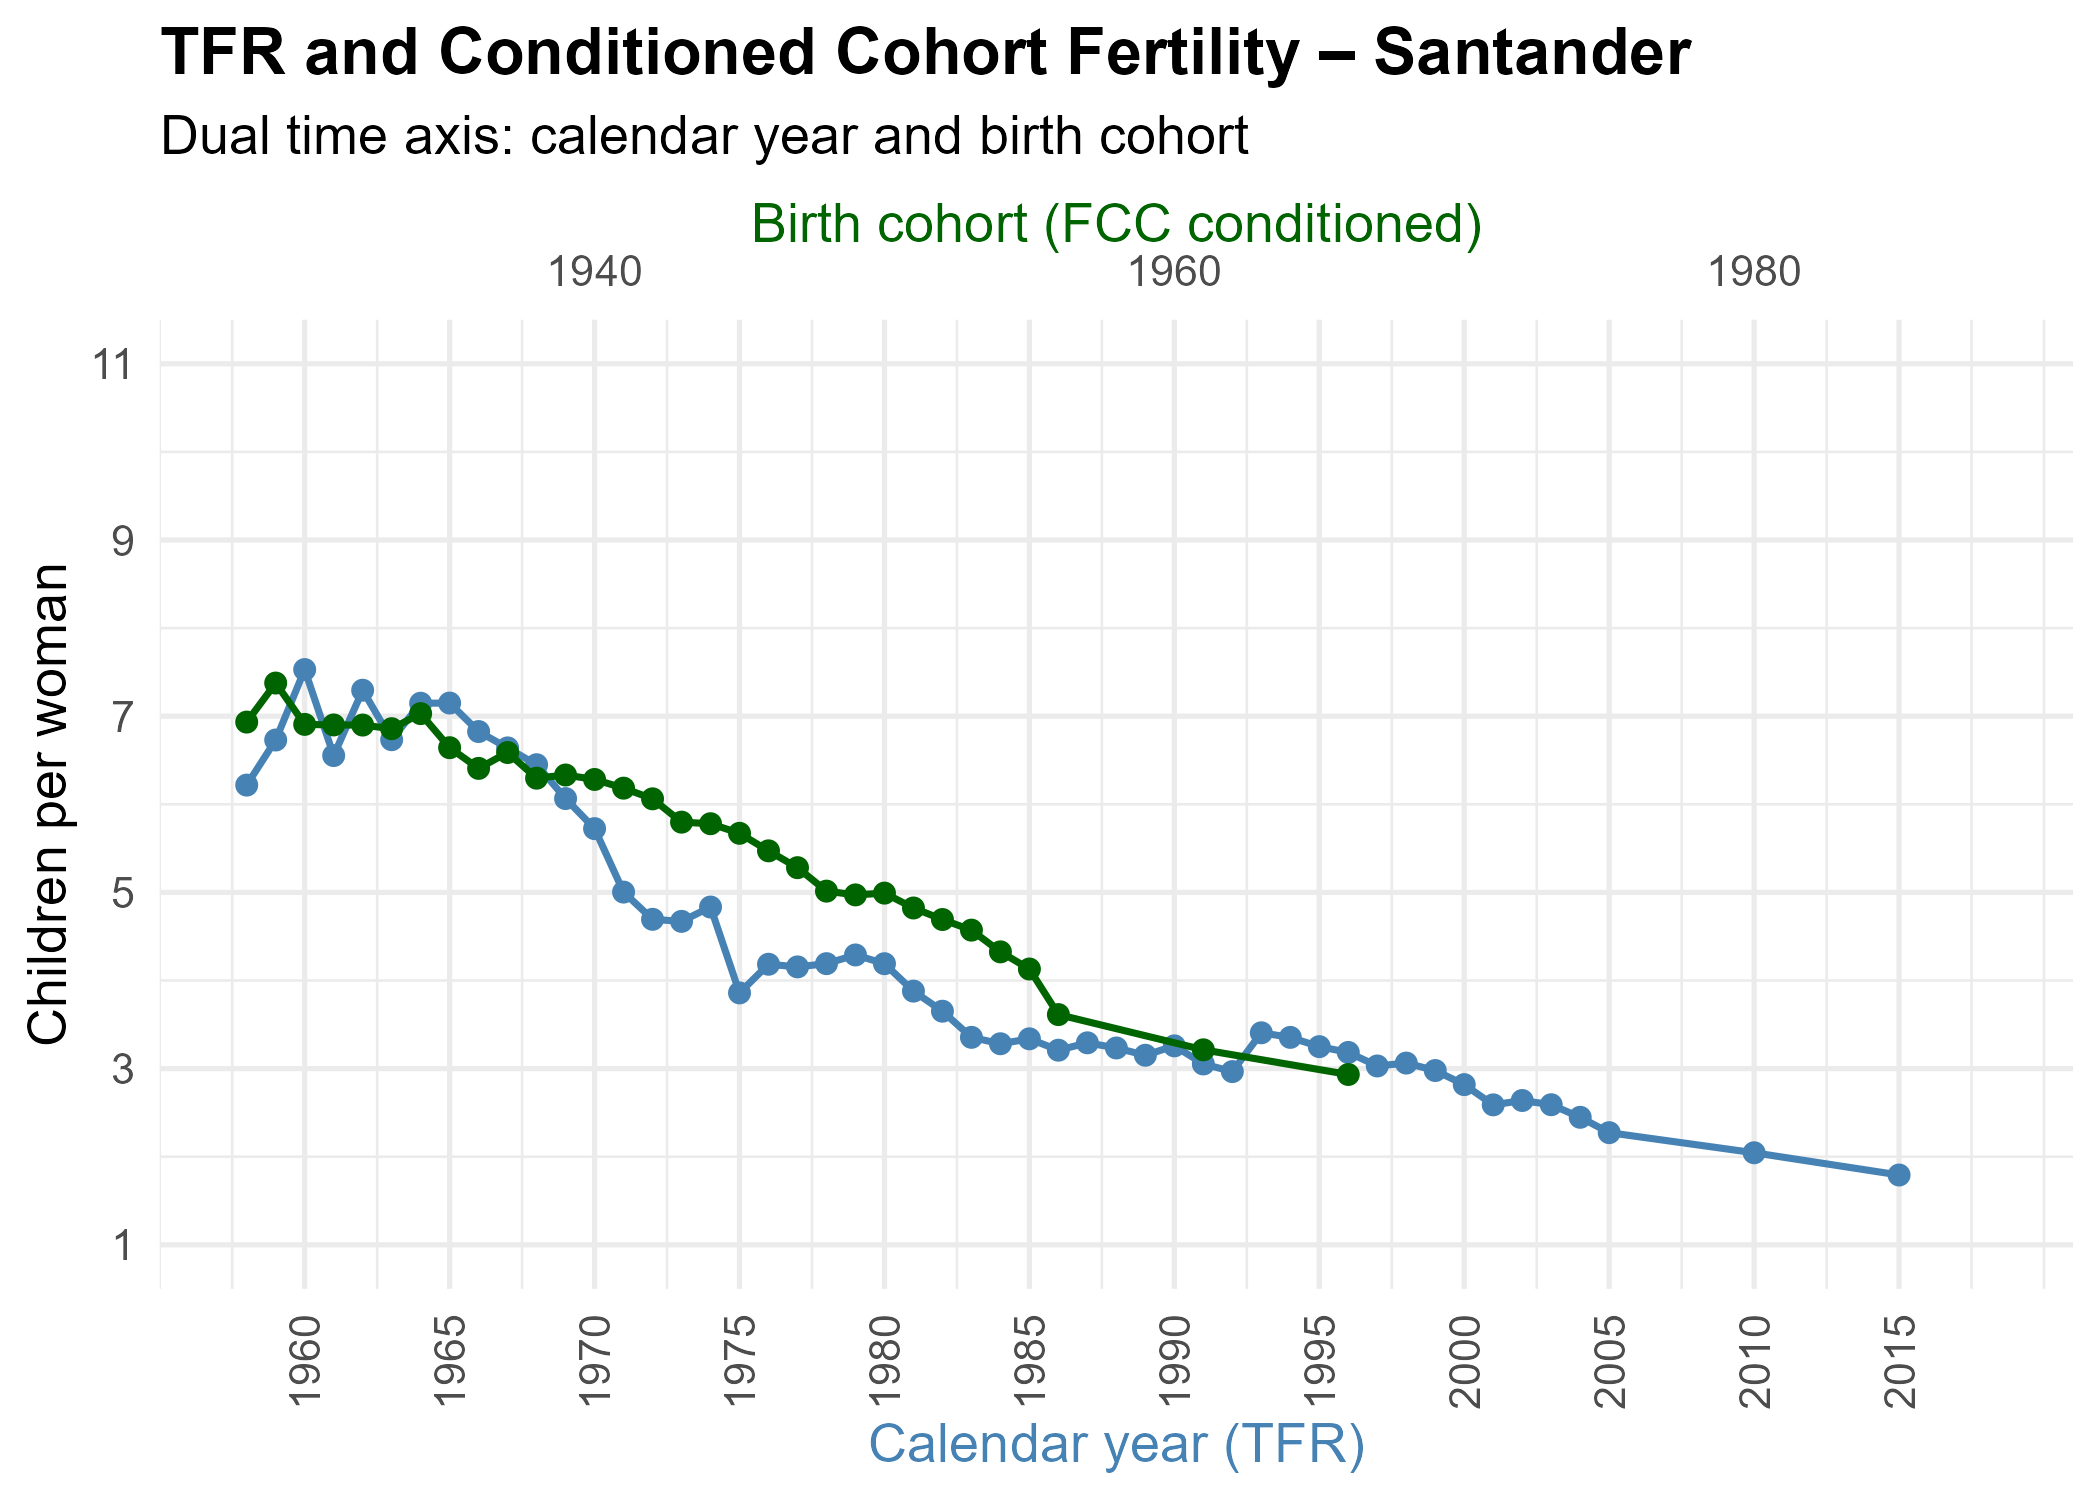
\includegraphics[height=0.78\textheight]{tfr_vs_fcc/TFR_FCCcond_Santander.png}
\end{center}
\end{frame}
\begin{frame}{TGF vs.\ FCC: Tolima}
\begin{center}
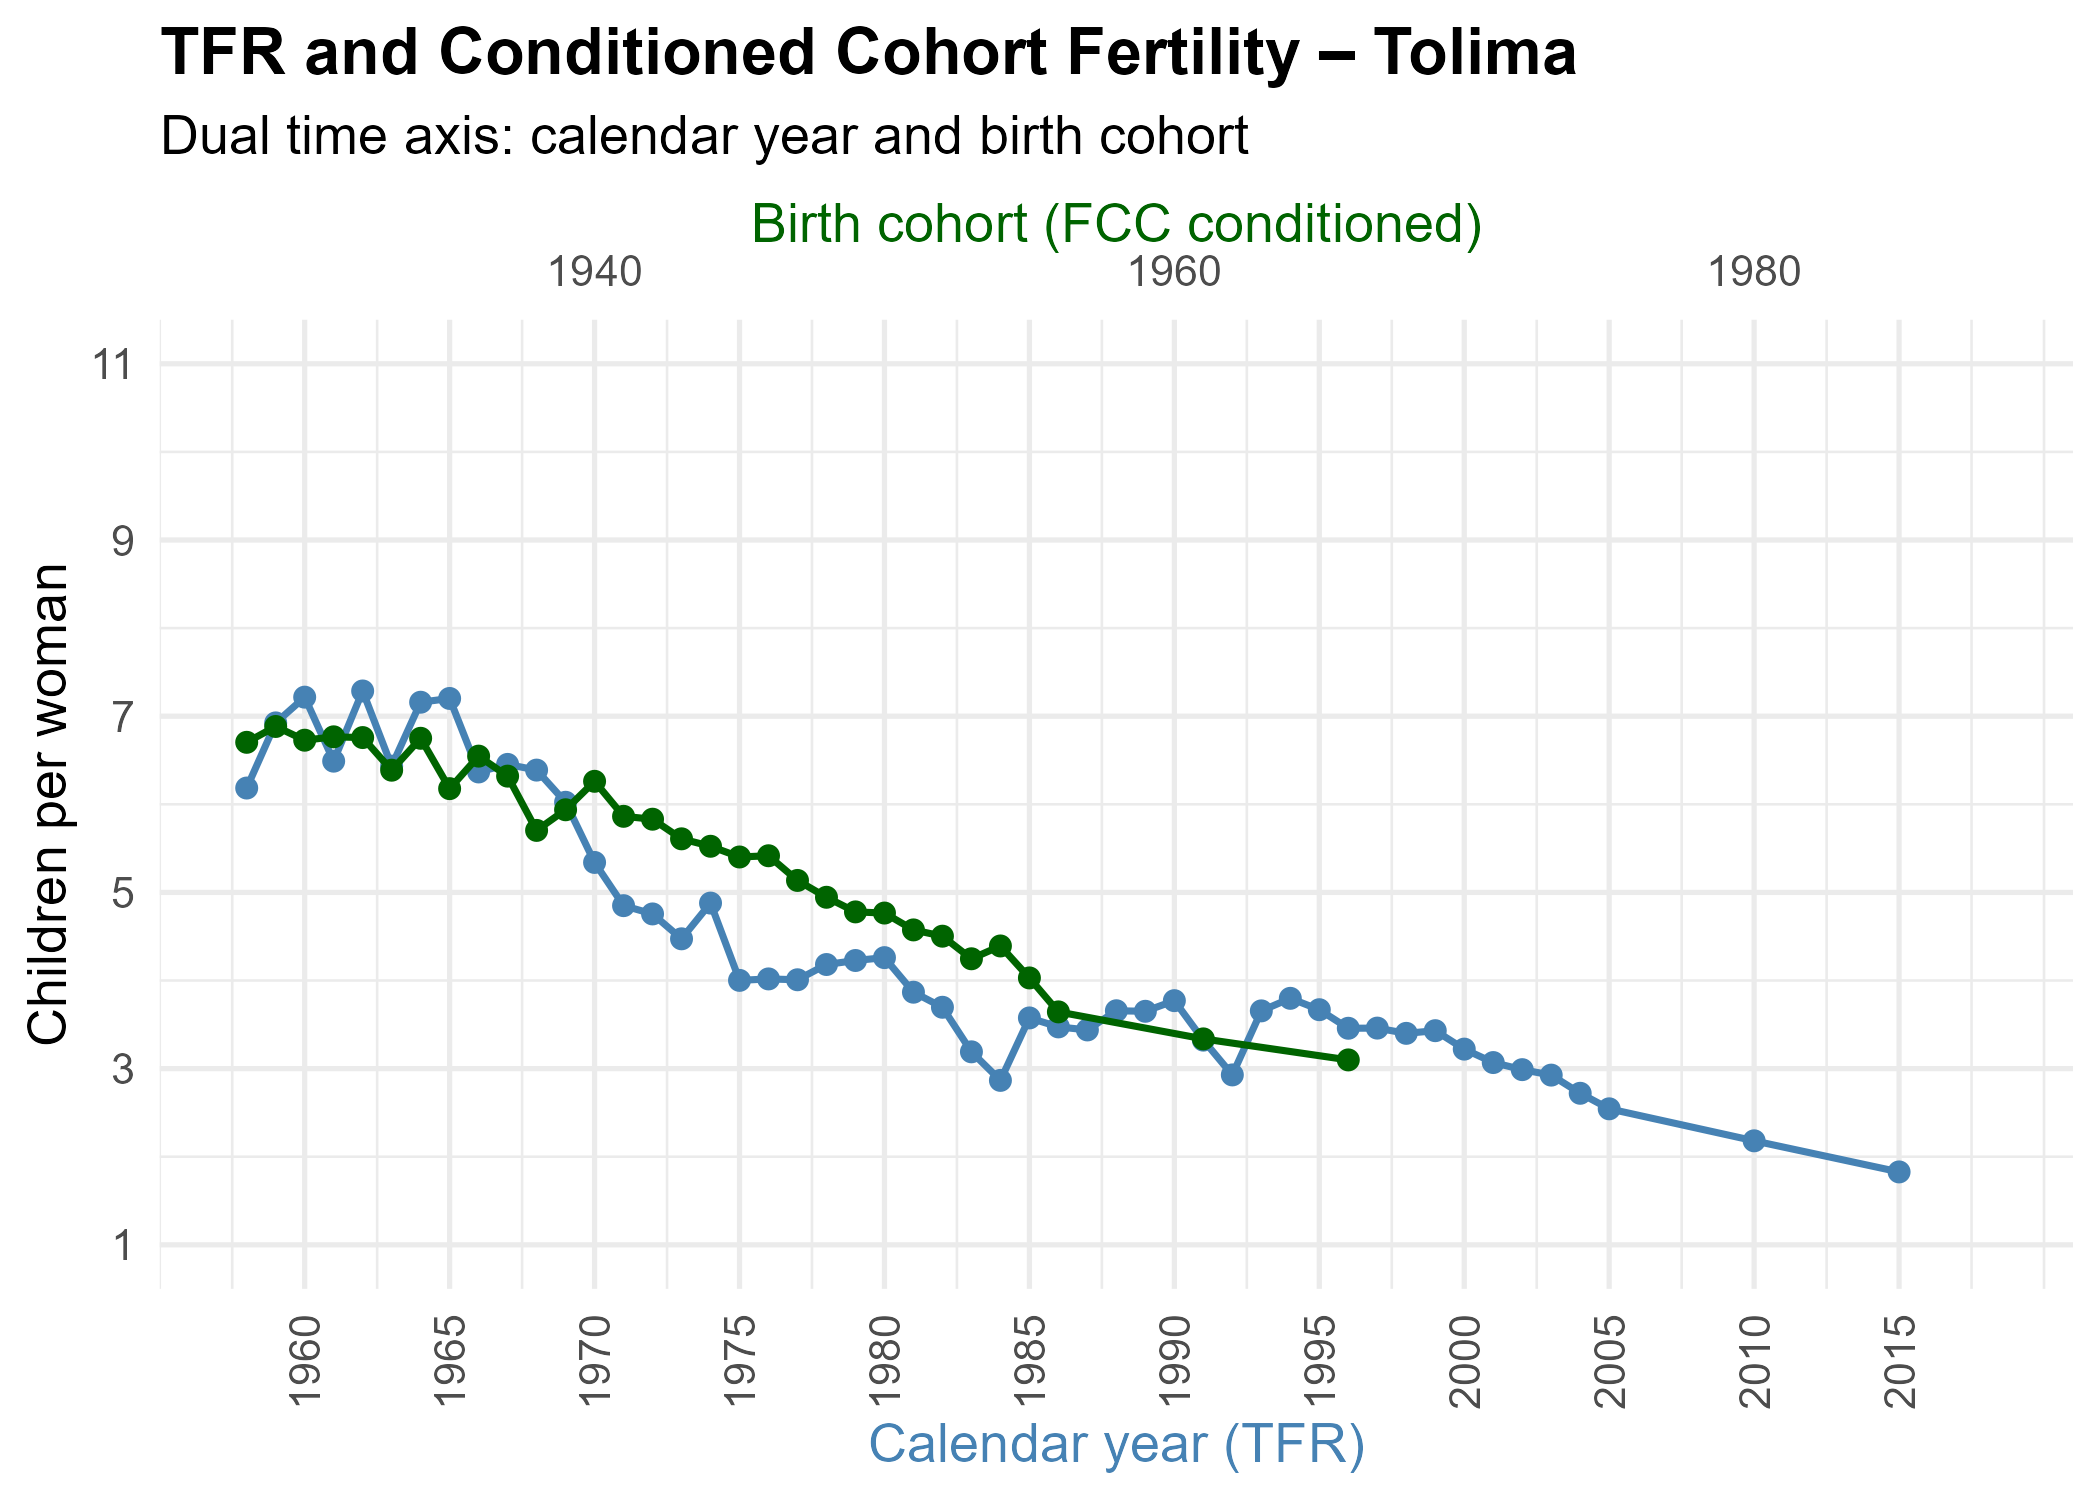
\includegraphics[height=0.78\textheight]{tfr_vs_fcc/TFR_FCCcond_Tolima.png}
\end{center}
\end{frame}
\begin{frame}{TGF vs.\ FCC: Valle del Cauca}
\begin{center}
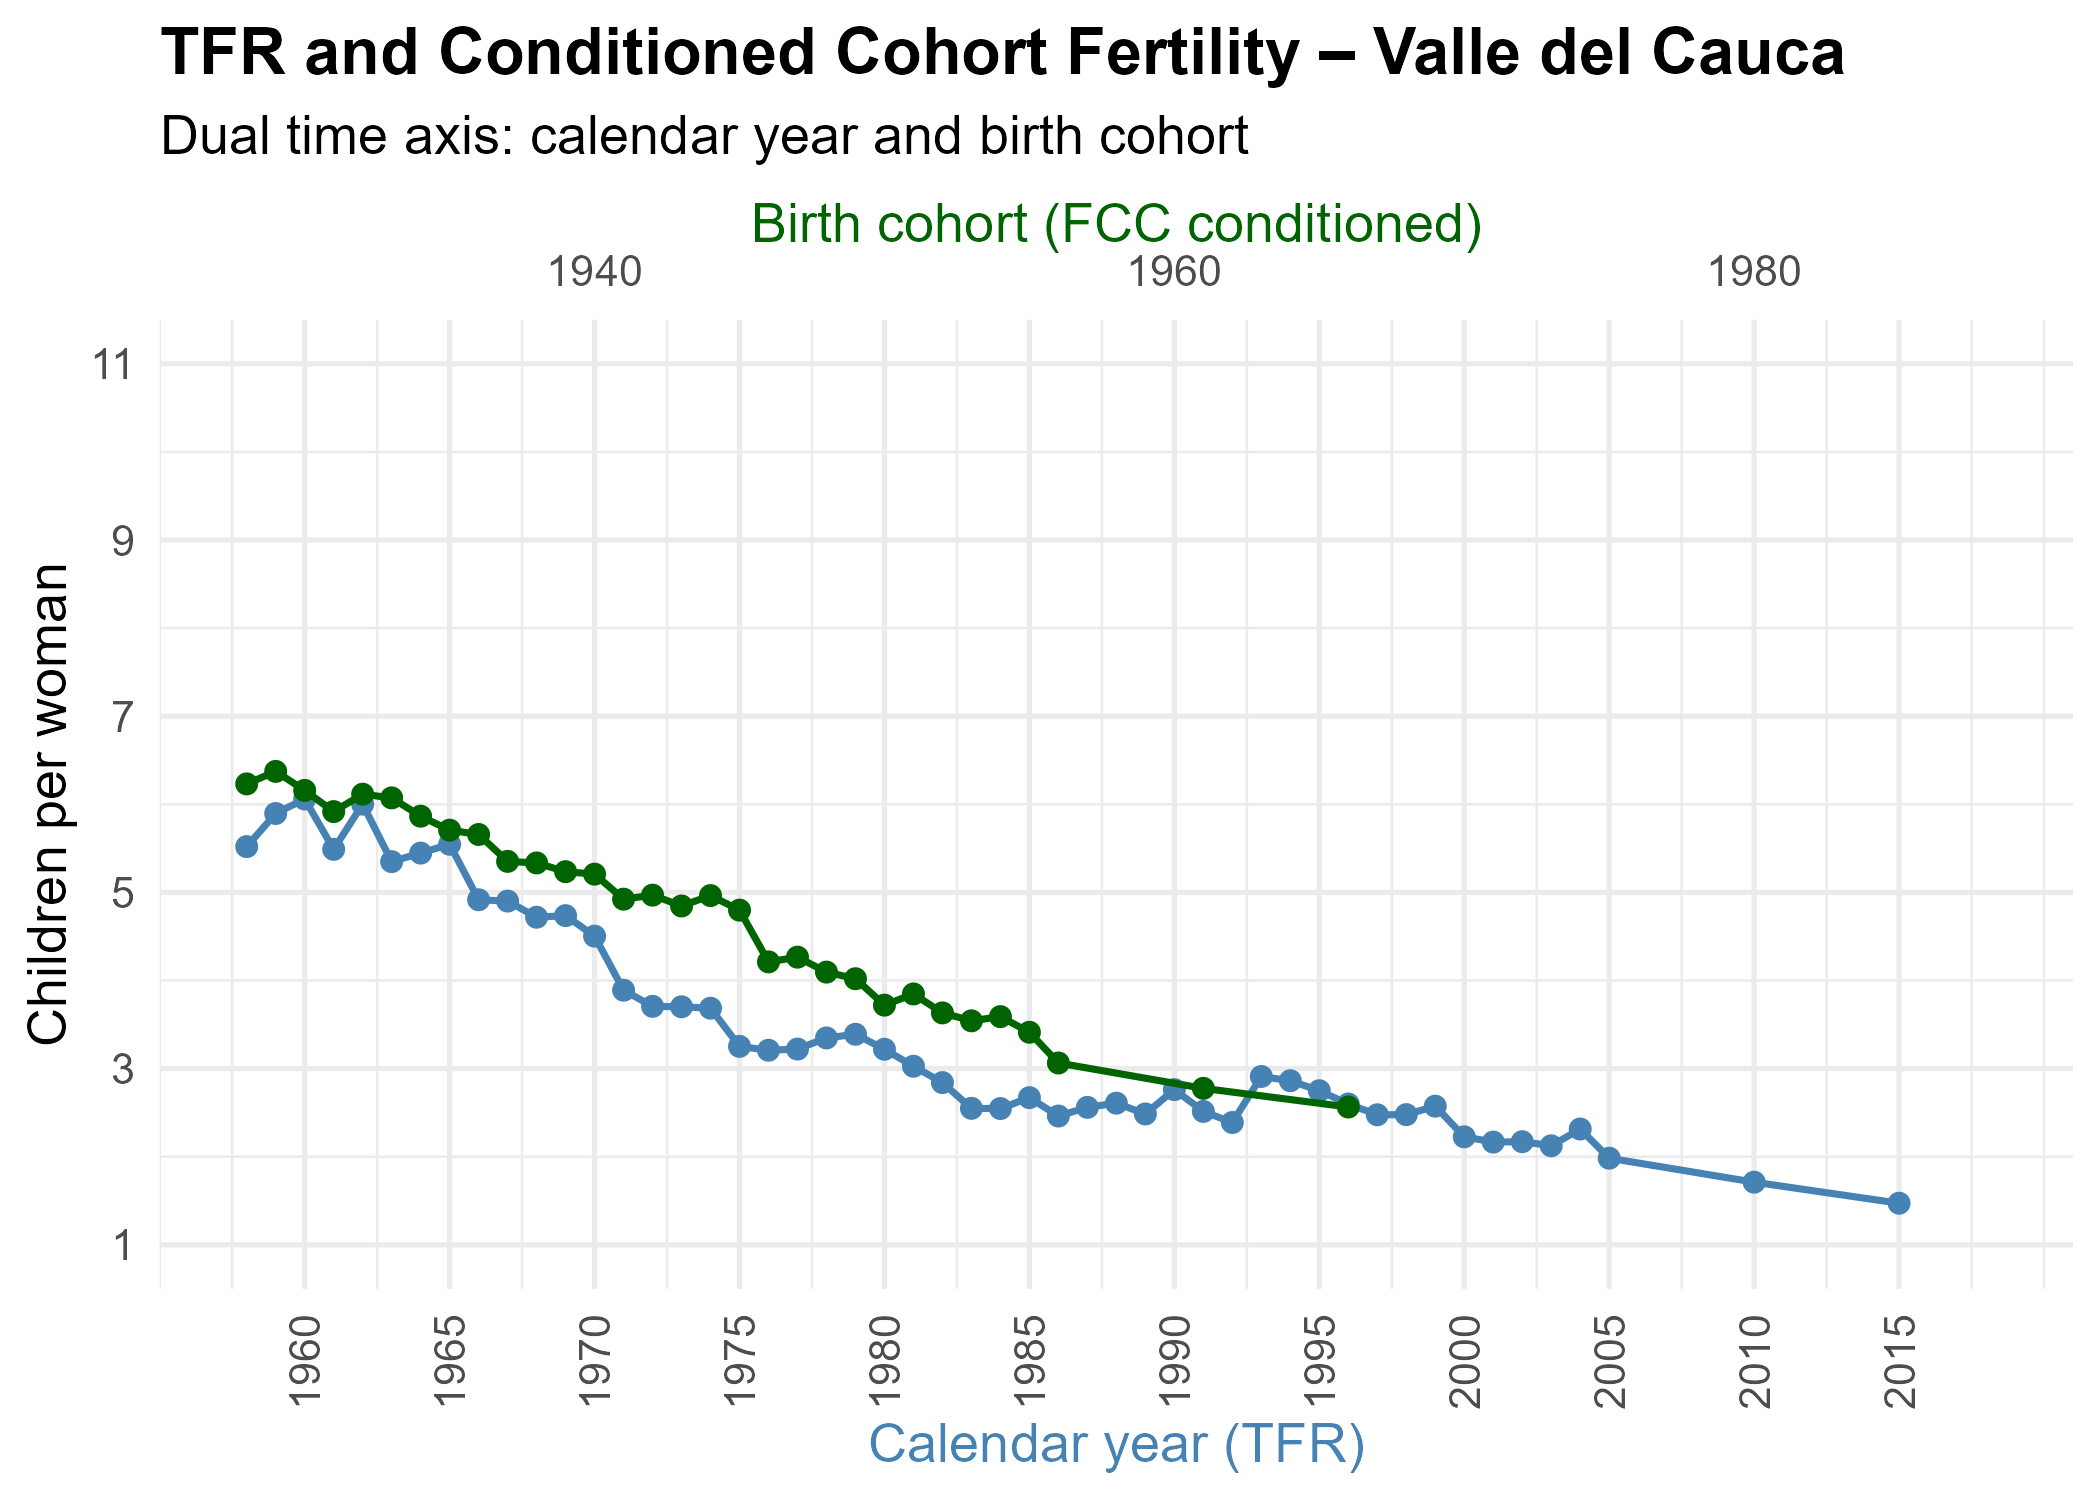
\includegraphics[height=0.78\textheight]{tfr_vs_fcc/TFR_FCCcond_Valle del Cauca.png}
\end{center}
\end{frame}
\section{Mujeres sin hijos}

\begin{frame}{Y crece el grupo que no tiene hijos}
\begin{columns}
\column{0.42\textwidth}
La transici\'on no es solo tener \emph{menos} hijos: tambi\'en m\'as
mujeres que no tienen \alert{ninguno}.
\medskip

El porcentaje de mujeres sin hijos entre 15 y 54 a\~nos aumenta censo
tras censo, especialmente en las edades centrales.
\column{0.5\textwidth}
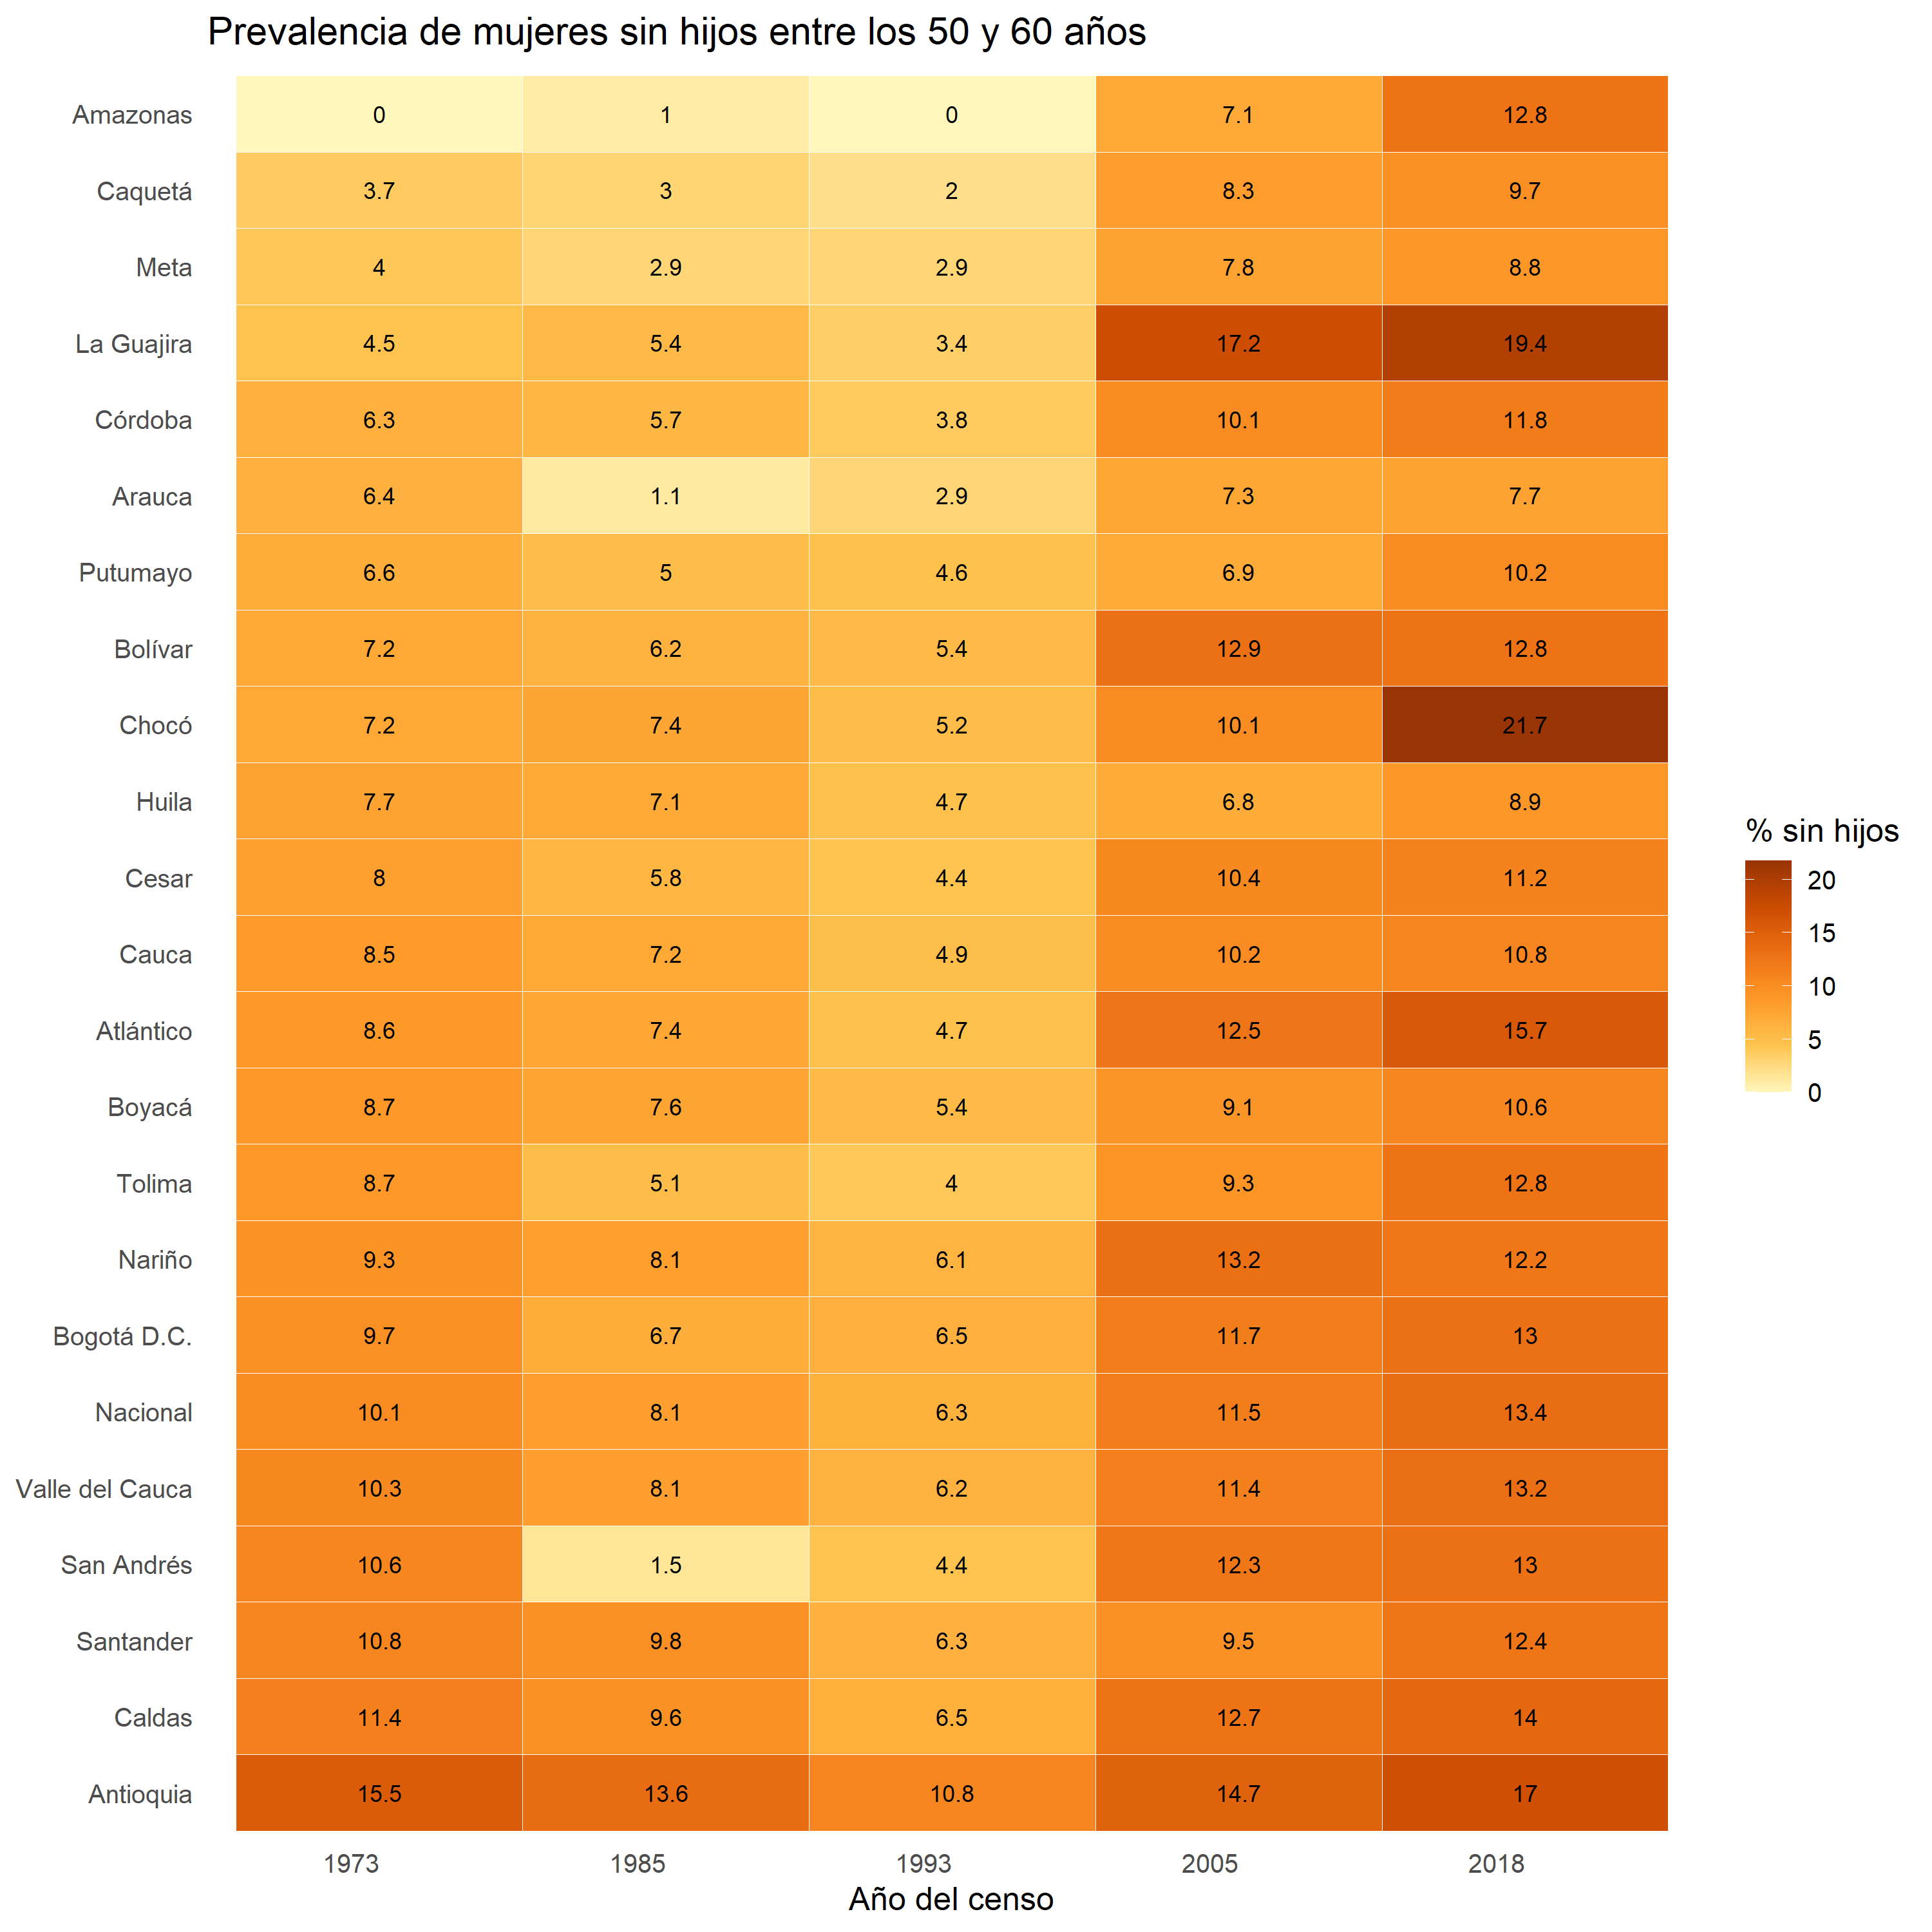
\includegraphics[width=\textwidth]{resumen/women_without_heatmap.png}
\end{columns}
\end{frame}

\section{Agenda}


\begin{frame}{Lo que sigue}
\begin{itemize}
\item Intervalos de confianza (bootstrap por hogares) como robustez.
\item Contraste con la ENDS y con el n\'umero de hijos declarado en el censo.
\item Explicar las desaceleraciones de 1997 y 2005 (literatura de
mortalidad infantil).
\item Convergencia formal; densidad poblacional y geograf\'ia
(cordillera) como correlatos.
\item Resolver San Andr\'es; afinar comparabilidad IPUMS,CNPV 2018.
\end{itemize}
\end{frame}


\end{document}
